%Input preamble
%Style
\documentclass[12pt]{article}
\usepackage[top=1in, bottom=1in, left=1in, right=1in]{geometry}
\parindent 22pt
\usepackage{fancyhdr}

%Packages
\usepackage{adjustbox}
\usepackage{amsmath}
\usepackage{amsfonts}
\usepackage{amssymb}
\usepackage{bm}
\usepackage[table]{xcolor}
\usepackage{tabu}
\usepackage{color,soul}
\usepackage{makecell}
\usepackage{longtable}
\usepackage{multirow}
\usepackage[normalem]{ulem}
\usepackage{etoolbox}
\usepackage{graphicx}
\usepackage{tabularx}
\usepackage{ragged2e}
\usepackage{booktabs}
\usepackage{caption}
\usepackage{fixltx2e}
\usepackage[para, flushleft]{threeparttablex}
\usepackage[capposition=top,objectset=centering]{floatrow}
\usepackage{subcaption}
\usepackage{pdfpages}
\usepackage{pdflscape}
\usepackage{natbib}
\usepackage{bibunits}
\definecolor{maroon}{HTML}{990012}
\usepackage[colorlinks=true,linkcolor=maroon,citecolor=maroon,urlcolor=maroon,anchorcolor=maroon]{hyperref}
\usepackage{marvosym}
\usepackage{makeidx}
\usepackage{tikz}
\usetikzlibrary{shapes}
\usepackage{setspace}
\usepackage{enumerate}
\usepackage{rotating}
\usepackage{tocloft}
\usepackage{epstopdf}
\usepackage[titletoc]{appendix}
\usepackage{framed}
\usepackage{comment}
\usepackage{xr}
\usepackage{titlesec}
\usepackage{footnote}
\usepackage{longtable}
\newlength{\tablewidth}
\setlength{\tablewidth}{9.3in}
\setcounter{secnumdepth}{4}

\titleformat{\paragraph}
{\normalfont\normalsize\bfseries}{\theparagraph}{1em}{}
\titlespacing*{\paragraph}
{0pt}{3.25ex plus 1ex minus .2ex}{1.5ex plus .2ex}
\makeatletter
\pretocmd\start@align
{%
  \let\everycr\CT@everycr
  \CT@start
}{}{}
\apptocmd{\endalign}{\CT@end}{}{}
\makeatother
%Watermark
\usepackage[printwatermark]{xwatermark}
\usepackage{lipsum}
\definecolor{lightgray}{RGB}{220,220,220}
%\newwatermark[allpages,color=lightgray,angle=45,scale=3,xpos=0,ypos=0]{Preliminary Draft}

%Further subsection level
\usepackage{titlesec}
\setcounter{secnumdepth}{4}
\titleformat{\paragraph}
{\normalfont\normalsize\bfseries}{\theparagraph}{1em}{}
\titlespacing*{\paragraph}
{0pt}{3.25ex plus 1ex minus .2ex}{1.5ex plus .2ex}

\setcounter{secnumdepth}{5}
\titleformat{\subparagraph}
{\normalfont\normalsize\bfseries}{\thesubparagraph}{1em}{}
\titlespacing*{\subparagraph}
{0pt}{3.25ex plus 1ex minus .2ex}{1.5ex plus .2ex}

%Functions
\DeclareMathOperator{\cov}{Cov}
\DeclareMathOperator{\corr}{Corr}
\DeclareMathOperator{\var}{Var}
\DeclareMathOperator{\plim}{plim}
\DeclareMathOperator*{\argmin}{arg\,min}
\DeclareMathOperator*{\argmax}{arg\,max}

%Math Environments
\newtheorem{theorem}{Theorem}
\newtheorem{claim}{Claim}
\newtheorem{condition}{Condition}
\renewcommand\thecondition{C--\arabic{condition}}
\newtheorem{algorithm}{Algorithm}
\newtheorem{assumption}{Assumption}
\renewcommand\theassumption{A--\arabic{assumption}}
\newtheorem{remark}{Remark}
\renewcommand\theremark{R--\arabic{remark}}
\newtheorem{definition}[theorem]{Definition}
\newtheorem{hypothesis}[theorem]{Hypothesis}
\newtheorem{property}[theorem]{Property}
\newtheorem{example}[theorem]{Example}
\newtheorem{result}[theorem]{Result}
\newenvironment{proof}{\textbf{Proof:}}{$\bullet$}

%Commands
\newcommand\independent{\protect\mathpalette{\protect\independenT}{\perp}}
\def\independenT#1#2{\mathrel{\rlap{$#1#2$}\mkern2mu{#1#2}}}
\newcommand{\overbar}[1]{\mkern 1.5mu\overline{\mkern-1.5mu#1\mkern-1.5mu}\mkern 1.5mu}
\newcommand{\equald}{\ensuremath{\overset{d}{=}}}
\captionsetup[table]{skip=10pt}
%\makeindex

\setlength\parindent{20pt}
\setlength{\parskip}{0pt}

\newcolumntype{L}[1]{>{\raggedright\let\newline\\\arraybackslash\hspace{0pt}}m{#1}}
\newcolumntype{C}[1]{>{\centering\let\newline\\\arraybackslash\hspace{0pt}}m{#1}}
\newcolumntype{R}[1]{>{\raggedleft\let\newline\\\arraybackslash\hspace{0pt}}m{#1}}



%Logo
%\AddToShipoutPictureBG{%
%  \AtPageUpperLeft{\raisebox{-\height}{
\includegraphics[width=1.5cm]{uchicago.png}}}
%}

\newcolumntype{L}[1]{>{\raggedright\let\newline\\\arraybackslash\hspace{0pt}}m{#1}}
\newcolumntype{C}[1]{>{\centering\let\newline\\\arraybackslash\hspace{0pt}}m{#1}}
\newcolumntype{R}[1]{>{\raggedleft\let\newline\\\arraybackslash\hspace{0pt}}m{#1}}

\newcommand{\mr}{\multirow}
\newcommand{\mc}{\multicolumn}

%\newcommand{\comment}[1]{}

%Other parameters
\newcommand{\noutcomes}{95}
\newcommand{\noutcomesexpp}{357}
\newcommand{\noutcomesexpm}{343}
\newcommand{\noutcomesexpf}{355}
\newcommand{\treatsubsabc}{$75\%$}
\newcommand{\treatsubscarec}{$74\%$}
\newcommand{\treatsubscaref}{$63\%$}

%Counts
%Males
\newcommand{\positivem}{$78\%$}
\newcommand{\positivesm}{$29\%$}

%Females
\newcommand{\positivef}{$78\%$}
\newcommand{\positivesf}{$31\%$}

%Counts, control substitution
%Males
\newcommand{\positivecsnm}{$47\%$}
\newcommand{\positivescsnm}{$15\%$}

\newcommand{\positivecsam}{$79\%$}
\newcommand{\positivescsam}{$29\%$}

%Females
%% no alternative
\newcommand{\positivecsnf}{$84\%$}
\newcommand{\positivescsnf}{$55\%$}

%% alternative
\newcommand{\positivecsaf}{$79\%$}
\newcommand{\positivescsaf}{$33\%$}

%Pooled

%Effects
%Males

%Females
\newcommand{\empf}{$8$}
\newcommand{\yearsedf}{$1.7$}



%Pooled

%CBA
%IRR
%Males
\newcommand{\irrm}{$15\%$}
\newcommand{\irrsem}{$5\%$}

%Females
\newcommand{\irrf}{$9\%$}
\newcommand{\irrsef}{$7\%$}

%Pooled
\newcommand{\irrp}{$13\%$}
\newcommand{\irrsep}{$5\%$}

%BC
%Males
\newcommand{\bcm}{$11.24$}
\newcommand{\bcsem}{$4.60$}

%Females
\newcommand{\bcf}{$2.35$}
\newcommand{\bcsef}{$1.09$}

%Pooled
\newcommand{\bcp}{$5.63$}
\newcommand{\bcsep}{$2.15$}

%NPV streams
%Pooled
\newcommand{\parincomenpvp}{$\$119,346$}

\externaldocument{abc_comprehensivecba_2016-08-01b_jlg.tex}
\pagenumbering{roman}

\begin{document}
\title{\Large \textbf{Appendix: \\ Analyzing the Short- and Long-term Effects of Early Childhood Education on Multiple Dimensions of Human Development}}

\author{
Jorge Luis Garc\'{i}a\\
The University of Chicago \and
James J. Heckman \\
American Bar Foundation \\
The University of Chicago \and
Andr\'{e}s Hojman\\
The University of Chicago \and
Duncan Ermini Leaf \\ 
University of Southern California \and
Mar\'{i}a Jos\'{e} Prados \\
University of Southern California \and
Joshua Shea \\
The University of Chicago \and 
Jake C. Torcasso \\
The University of Chicago}
\date{First Draft: January 5, 2016\\ This Draft: \today}
\maketitle
\thispagestyle{empty}

%\pagebreak
\tableofcontents
\listoffigures
\listoftables
\pagebreak
\doublespacing

%Input Appendices
\pagenumbering{arabic}
\begin{appendices}
\setcounter{figure}{0}  \renewcommand{\thefigure}{A.\arabic{figure}}
\setcounter{table}{0}   \renewcommand{\thetable}{A.\arabic{table}}

\section[Background]{Background\footnote{This section of the appendix is based on joint work with Sylvi Kuperman.}} \label{appendix:background}

\subsection{Overview}

\noindent The Carolina Abecedarian Project (ABC) and the Carolina Approach to Responsive Education (CARE) were high-quality early childhood education programs each with two phases of randomized controlled design. They were both implemented at the Frank Porter Graham Center (FPGC) of the University of North Carolina in Chapel Hill. ABC served four cohorts of children born between 1972 and 1977, and CARE served two cohorts of children born between 1977 and 1980. In the main paper, we explain the eligibility requirements, the randomization protocol, and the programmatic contents of both programs. In this section of the appendix, we expand on additional important details of all these aspects.

\subsection{Eligibility Criteria and Populations Served}

\noindent The mothers of the ABC and CARE subjects were typically recruited during the last trimester  of pregnancy. Potential families were referred by local social service agencies and hospitals. Eligibility was determined by a score of 11 or more on a weighted 13-factor High-risk Index (HRI).\\ 

\noindent The HRI for ABC was based on 13 weighted variables, which are listed here with weights in parentheses: (i) maternal education level measured by years of education--- 6 (8), 7 (7), 8 (6), 9 (3), 10 (2), 11 (1), 12 (0); (ii) paternal education level with weights identical to those for maternal education; (iii) yearly family income measured in current dollars---\$1,000 or less (8), \$1,001-\$2000 (7), \$2,001-\$3,000 (6), \$3,001-\$4,000 (5), \$4,001-\$5,000 (4), \$5,001-\$6,000 (0); (iv) father's absence from the household for reasons other than health or death (3); (v) lack of maternal relatives in the area (3); (vi) siblings of school age one or more grades behind age-appropriate level, or with equivalently low scores on school-administered achievement tests (3); (vii) received payments from welfare agencies within the past 3 years (3); (viii) record of father's work indicates instability or unskilled and semi-skilled labor (3); (ix) record of maternal or paternal IQ score of 90 or below (3); (x) record of a sibling with an IQ score of 90 or below (3); (xi) relevant social agencies in the community indicate the family is in need of assistance (3); (xii) one or more family members has sought counseling or professional help in the past 3 years (1); and (xiii) special circumstances not included in any of the above that are likely contributors to cultural or social disadvantage (1).\footnote{\citet{Ramey_Smith_1977_AJMD, Ramey_Campbell_1984_AJMD,Ramey_Campbell_1991_childreninpoverty,Ramey_Campbell_etal_2000_ADS}.} The weighting scale aimed to establish the relative importance of each item in the index.\footnote{\citet{Ramey_Smith_1977_AJMD}.} Race was not  considered for eligibility; however, 98\% of the families who agreed to participate were African-American.\footnote{\citet{Ramey_Smith_1977_AJMD,Ramey_Campbell_1979_SR}.} \\

\noindent The HRI for CARE was similar to that of ABC---it also contained 13 weighted variables and a score of 11 or above was required to be considered eligible. The items for maternal and paternal education levels have the same categories and weights as the ABC HRI. The other identical items are having an absent father,  school-age siblings performing lower than the norm based on grade-level or achievement tests, a record of father's unstable job history or unskilled labor, social agencies indicating a high level of need, and other circumstances related to cultural or social disadvantage. The specification of the following items were changed between the ABC and CARE HRI. The weight associated with household income depended on the number of individuals in the family for CARE and the income categories range from less than \$2,000 to \$13,500 or more. In the CARE HRI, it is asked if payments were received from welfare agencies in the past 5 years instead of the past 3 years. Similarly, it asks if any family member has sought counseling in the past 5 years instead of the past 3 years. The threshold for maternal or paternal IQ is 85 in the CARE HRI instead of 90 as in the ABC HRI.  It does not have an item related to the absence of maternal relatives in the area, but replaces that item with asking if any member of the mother or father's immediate family has received services for the mentally disabled (the weight for this item is 3).\footnote{\citet{Ramey_etal_1985_Project-CARE_TiECSE}.}
\begin{center}
	\begin{figure}[H]
		\caption{High-risk Index Distribution, ABC} \label{figure:hridistabc}
		\centering
		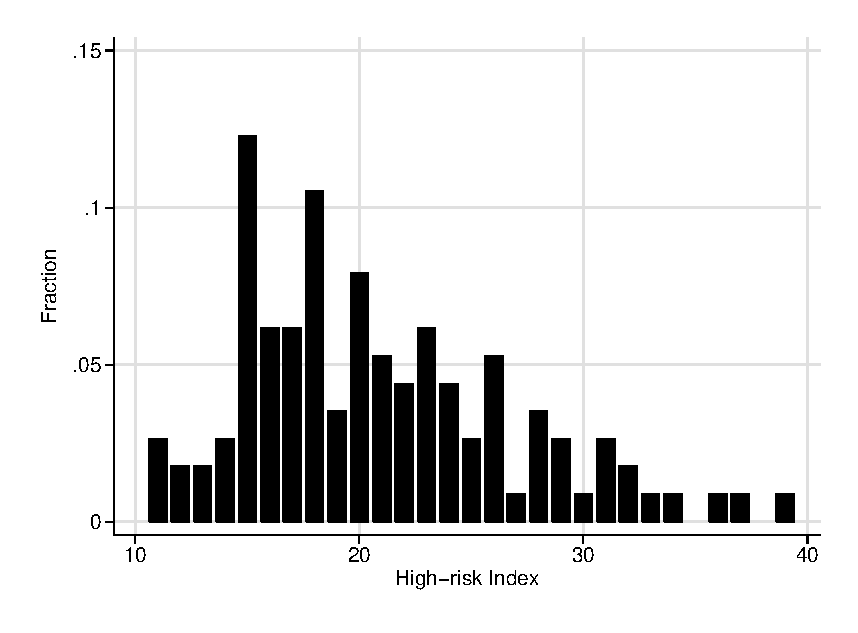
\includegraphics[width=.9\columnwidth]{output/abc_hri.eps}
\floatfoot{
\footnotesize
\noindent Note: This plot shows the distribution of the High-risk Index (HRI) for ABC, which determined eligibility. Subjects were eligible if they had a score of 11 or more.}
	\end{figure}
\end{center}

\begin{center}
	\begin{figure}[H]
		\caption{High-risk Index Distribution, CARE} \label{figure:hridistcare}
		\centering
		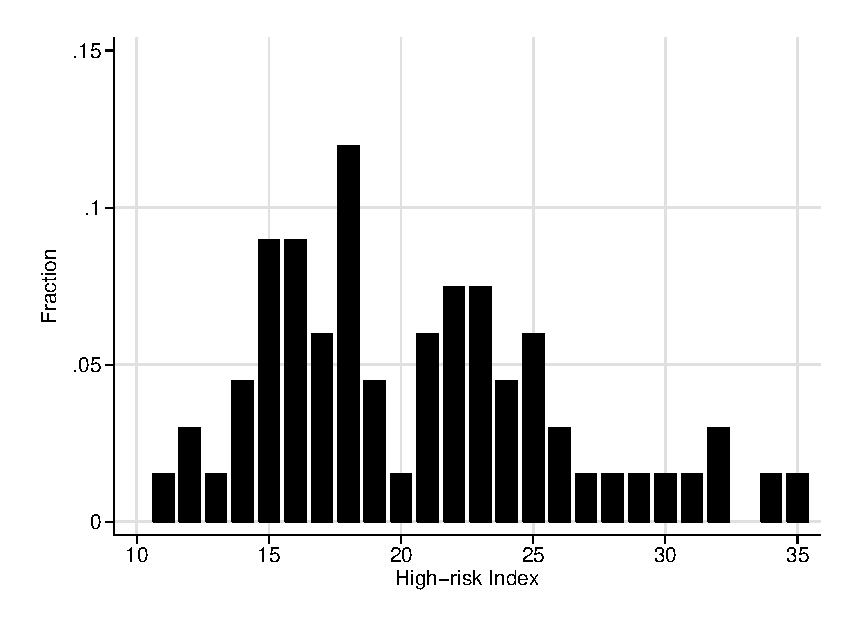
\includegraphics[width=.95\columnwidth]{output/care_hri.eps}
\floatfoot{
\footnotesize
\noindent Note: This plot shows the distribution of the High-risk Index (HRI) for CARE, which determined eligibility. Subjects were eligible if they had a score of 11 or more.}
	\end{figure}
\end{center}

\noindent Figure~\ref{figure:hridistabc} and Figure~\ref{figure:hridistcare} display the distribution of the HRI score among all subjects in ABC and CARE, respectively. All subjects were substantially disadvantaged. Maternal age when the subject was born was, on average, 19.9 years in ABC and 21.1 years in CARE. Approximately half of the mothers of both treatment-group and control-group subjects in ABC were 19 years or younger and one third were 17 years or younger. In CARE, approximately half of the mothers of both treatment-group and control-group subjects were 20 years or younger and one third were 17.2 years or younger.  Mean maternal IQ score in ABC was approximately 85, one standard deviation below the national mean. In CARE, the mean maternal IQ score was approximately 87. Only 25\% of the ABC subjects lived with both biological parents, and more than 50\% lived with extended families in multi-generational households (61\% of treatment-group subjects and 56\% of control-group subjects).\footnote{\citet{Ramey_Campbell_1991_childreninpoverty,Campbell_Ramey_1994_CD}.} About 79\% of subjects did not have a father in the home in both ABC and CARE. \\

\subsection{Randomization Protocol and Compromises} \label{appendix:randomization}

\noindent Randomization compromises throughout ABC's and CARE's implementations pose a challenge when evaluating the programs' effects. We discuss each case of compromise in detail. Figure~\ref{fig:abc-flow} and Figure~\ref{fig:care-flow} are flow charts that depict the sample from the first-phase randomization through the last data follow-up accounting for all cases of attrition and non-compliance. In Section~\ref{section:methodology},  we propose a methodology for adequately evaluating the programs while accounting for these compromises.\\

\noindent Although most randomization compromises occurred at early stages, this methodology also accounts for the fact that a few subjects were not in the sample either for the second-phase randomization or for the adult follow-ups. In Appendix~\ref{appendix:data}, we describe the sample reductions that attrition at different stages of the study generates and test potential differences between the subjects who completed data follow-ups and the subjects who did not.\\


\begin{center}
	\begin{figure}[H]
		\caption{Randomization Protocol and Treatment Compliance, ABC} \label{fig:abc-flow}
		\centering
		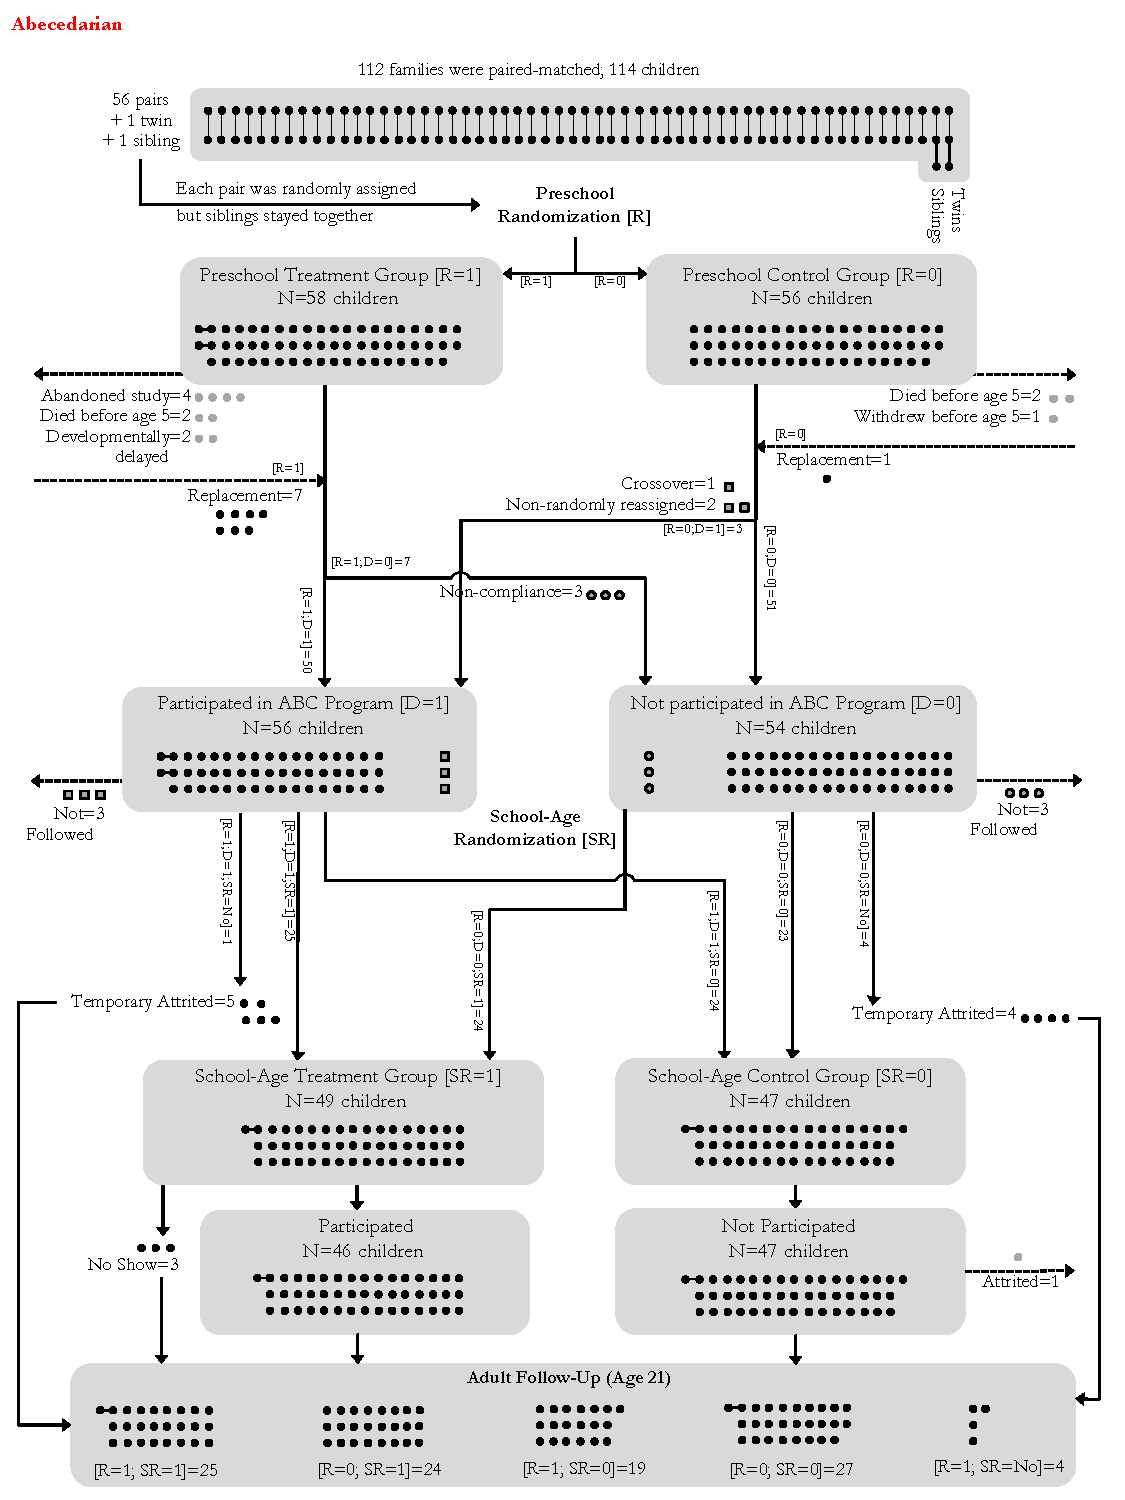
\includegraphics[width=.7\columnwidth]{output/abc_Diagram.pdf}
\floatfoot{
\footnotesize
\noindent
Sources: \cite{Ramey_Collier_etal_1976_CarolinaAbecedarianProject, Ramey_Smith_1977_AJMD,Ramey_Campbell_1979_SR,Ramey_Campbell_1984_AJMD}, internal documentation of the program, and own calculations. Note: The variable $R$ represents randomization into treatment, $[R=1]$, or control, $[R=0]$, groups. After the original randomization, some subjects died or withdrew from the program early in life and were replaced. $R$ also includes those replacements. Arrows pointing outside of the diagram indicate subjects who left the study permanently. The variable $P$ represents participation in the preschool-age program. The variable $SR$ represents randomization into the school-age program, $[SR=1]$, or out of it, $[SR=0]$. Some subjects were not randomized at school age, $[SR=No]$. We use the term ``temporarily attrited" for subjects who did not participate in the study at school age, but were later interviewed in the age-21 followup.
}
	\end{figure}
\end{center}

\begin{center}
	\begin{figure}[H]
		\caption{Randomization Protocol and Treatment Compliance, CARE} \label{fig:care-flow}
		\centering
		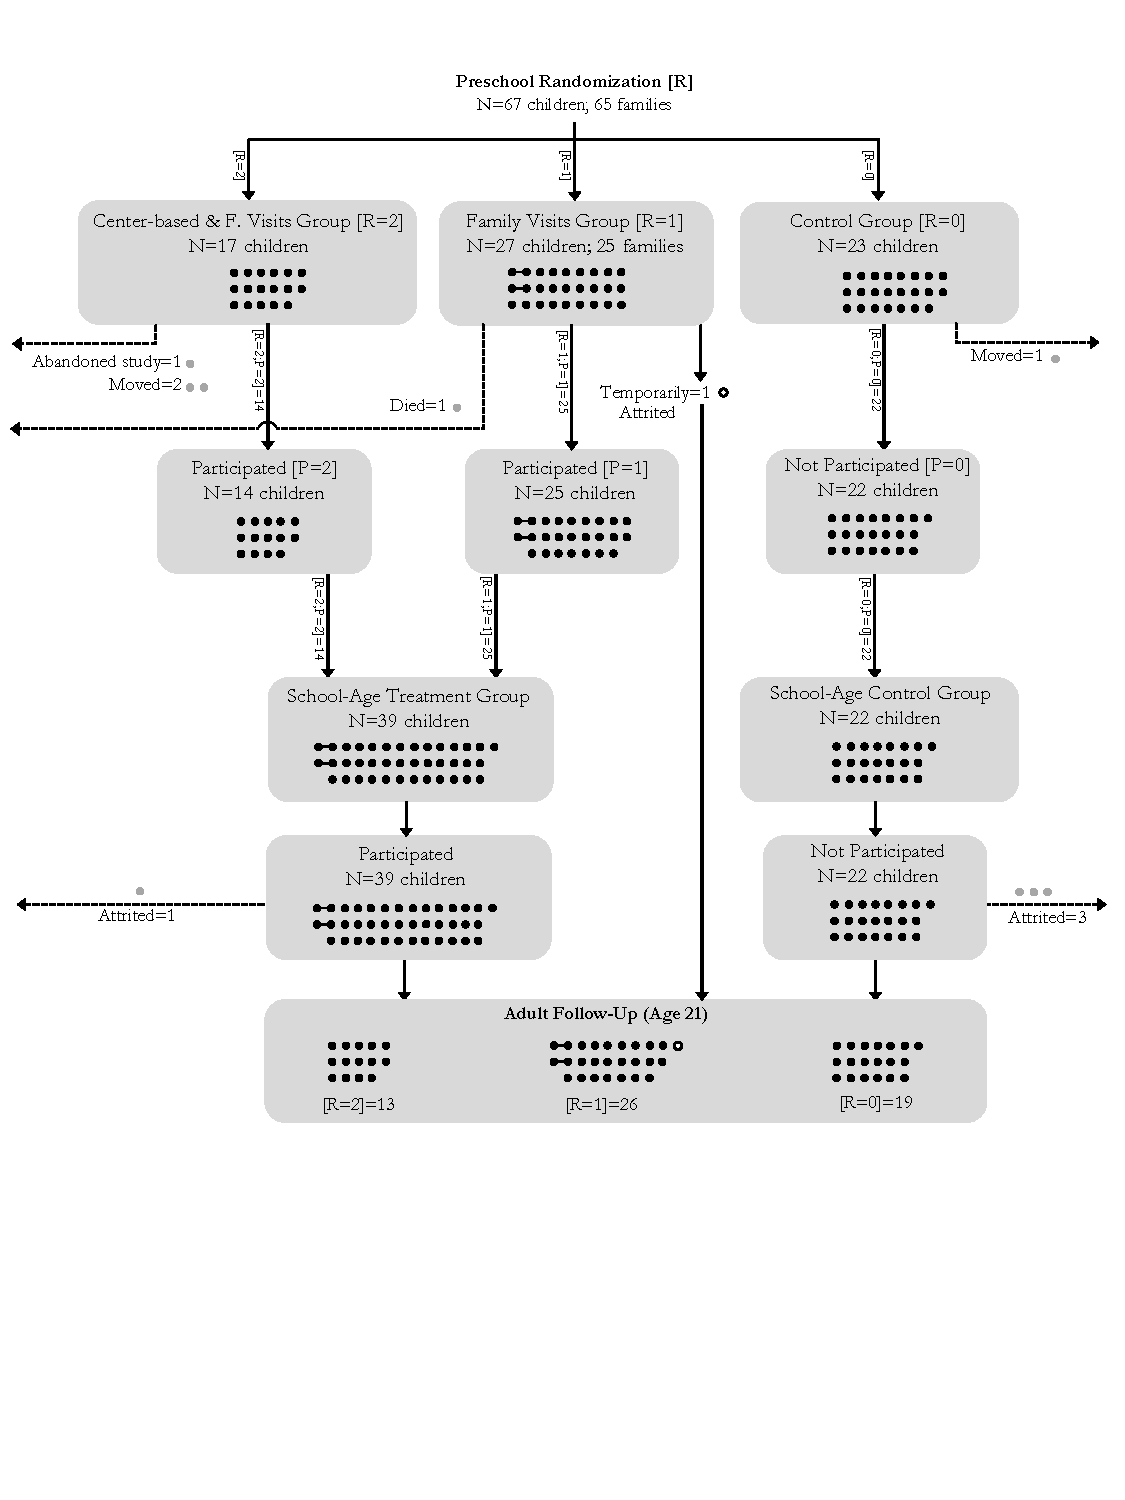
\includegraphics[width=.8\columnwidth]{output/care_Diagram.pdf}
\floatfoot{
\footnotesize
\noindent
Sources: \cite{Wasik_Ramey_etal_1990_CD}, internal documentation of the program, and own calculations. Note: The variable $R$ represents randomization into center-based childcare and family education, $[R=2]$, family education, $[R=1]$, or control, $[R=0]$. Arrows pointing outside of the diagram indicate subjects who left the study permanently. The variable $P$ represents participation in the corresponding group of the preschool-age program. The variable $SR$ represents those who participated in the school-age program, $[SR=1]$, or did not, $[SR=0]$. Unlike in ABC, there was no second-phase randomization in CARE. Rather, those in the center-based childcare and family education group and those in the family education group were automatically assigned to receive the school-age treatment. We use the term ``temporarily attrited" for subjects who did not participate in the study at school age, but were later interviewed in the age-21 followup.
}
	\end{figure}
\end{center}

\subsubsection{ABC}

\noindent Both the first and second phases of randomization were conducted at the family level, so pairs of siblings and twins were jointly randomized into either treatment or control groups.\footnote{Sibling pairs occurred when the two siblings were close enough in age such that both of them were eligible for the program.} Although we know that pairing was based on HRI, maternal IQ, maternal education, maternal age, and gender of the subject, we do not know the original pairs. The study collected an initial sample of 120 families. Twenty-two subjects did not complete the first-phase of treatment as initially assigned by the randomization (see Table~\ref{table:abccompromises}).\footnote{In Appendix~\ref{appendix:controls}, we compare the observed baseline characteristics of the subjects in Table~\ref{table:abccompromises} to the observed baseline characteristics of the subjects who complied to the initial treatment assignment. We find little evidence of differences.}\\


\noindent Of these cases, there were four subjects assigned to treatment who left the study before any data on them was collected. In our main methodology, we assume that they are missing at random. Exercises assuming that these subjects had outcomes identical to the subject with the lowest outcome in the treatment group suggest that, even in this extreme scenario, there is little sensitivity (see Appendix~\ref{appendix:assessingcc}).\\

\noindent Second, four subjects died before age 5---two of them initially assigned to treatment and two of them initially assigned to control. For all of them, we observe baseline characteristics and any other data collected before their death. For methodological purposes, they represent cases of program attrition when we do not observe their outcomes.\\

\noindent Third, three subjects in the treatment group did not comply to treatment status. They are different from the four subjects who left the study before any data collection because we observe data collected for them from birth to age 8. Afterward, the program staff chose not to follow them anymore.\footnote{Informal conversations with the program's staff do not indicate a clear reason for this.} Therefore, these subjects remain in treatment sample until age 8 or before. After, they represent cases of program attrition, given that we do not observe them anymore. In Appendix~\ref{appendix:assessingcc} we find little sensitivity to adjusting for non-compliance of these children in the results we show for age 8 or before.\\

\begin{sidewaystable}[H] 
\begin{threeparttable}
\caption{Randomization Compromises, ABC}
\label{table:abccompromises}
\centering
\footnotesize
\begin{tabular}{ccccc} \toprule
Child ID & Initial Assignment & Compromise Description & Data Availability & Methodology Assumption \\ \\ \midrule
Case A & Treatment & Left the study & None & Missing at random \\
Case B & Treatment & Left the study & None & Missing at random \\
Case C & Treatment & Left the study & None & Missing at random \\
Case D & Treatment & Left the study & None & Missing at random \\ \midrule
.x    & Control  & Died (age 0), heart disease & Baseline; before dead & Attrition after death \\
914 & Control  & Died (age 0), heart disease & Baseline; before dead & Attrition after death \\
74 & Treatment & Died (age 0), SIDS & Baseline; before dead & Attrition after death \\
99 & Treatment  & Died (age 4), pedestrian accident & Baseline; before dead & Attrition after death \\ \midrule
900 & Treatment  & Non-compliance  & Baseline; before age 8 & Attrition after age 8  \\
912 & Treatment  & Non-compliance  & Baseline; before age 8 & Attrition after age 8  \\
922 & Treatment  & Non-compliance  & Baseline; before age 8 & Attrition after age 8  \\ \midrule
78  & Control        & Crossover from control to treatment & Baseline; before age 8 & Attrition after age 8  \\ \midrule
85 & Treatment   & 3 months of treatment &  Baseline; after age 2 & Same as treatment group  \\  
103 & Treatment &10 months of treatment &  Baseline; after age 2 & Same as treatment group  \\
108 & Treatment & 6 months of treatment &  Baseline; after age 2 & Same as treatment group  \\ 
123 & Treatment & 9 months of treatment &  Baseline; after age 2 & Same as treatment group  \\  \midrule
906 & Control  & Left study at 54 months & Baseline; before 54 months & Attrition after 54 months \\ \midrule
95   & Treatment       & Developmentally delayed at 6 months & No data after diagnosis & Dropped (non-eligible) \\ 
124 & Treatment       & Developmentally delayed at 36 months & No data after diagnosis & Dropped (non-eligible) \\ \midrule
 82 & Control       & Crossover from control to treatment & Baseline, before age 8 & Dropped (non-eligible)  \\ 
 119 & Control       & Crossover from control to treatment & Baseline, before age 8 & Dropped (non-eligible)  \\ \bottomrule
\end{tabular}
\begin{tablenotes}
\item Note: This table describes the various randomization compromises in ABC. For each child, we display: the ID assigned by the program staff, the nature of the compromise, the data available, and the methodological assumption when accounting for non-compliance and program attrition. 
\end{tablenotes}
\end{threeparttable}
\end{sidewaystable}

\noindent Fourth, one subject initially assigned to control was enrolled into treatment. Her mother wanted to work and the program staff decided to admit her child into center-based care.\footnote{Correspondence with the program officers stating this permission is available under request from the authors.} Both in terms of data collection and in terms of methodological purposes, this subject is analogous to the subjects in the third case.\footnote{The sensitivity analysis finding little evidence when adjusting for non-compliance includes this case.}\\

\noindent Fifth, four subjects in the treatment group did not complete treatment in its entirety. They were treated for 3, 10, 6, and 9 months, respectively. Except for follow-ups during childhood, which our main results do not use, we observe most of the data for these subjects. We avoid taking a stance on how beneficial the program was at each age, because we do not have a way to document this. Therefore, we assume that they were treated as other subjects in the treatment group.\footnote{If anything, this downward biases the effects of the program we estimate.} \\

\noindent Sixth, the family of one subject in the control group moved at age 54 months. We observe any data collection before the family moved, so we consider the subject as part of the control group in any estimation before this event. Afterwards, we do not observe any data on the subject, so we consider her a case of program attrition.\\

\noindent Seventh, two subjects initially assigned to treatment status were diagnosed as developmentally delayed after 6 and 36 months of treatment. No data for them are available after the diagnosis. We drop them from the sample because they were not eligible to be part of the program.\\

\noindent Finally, two subjects initially assigned to the control group were admitted into treatment. Local authorities requested this because the children were considered highly at risk. Data on them are available from birth to age 8 and we treat them as the subjects in the third and fourth cases. They crossed over from the control group to the treatment group, although the reasons were different.\\

\noindent Analysis of each of these cases leads to the following conclusions. For four subjects, we do not have data to methodologically assess them as cases of program attrition, though sensitivity analyses suggest that the treatment effects of the program persist after assigning them the same outcome as the subjects who did the worst in the treatment group. For the subjects who did not comply to treatment, adjusting our estimates for non-compliance when data are available makes little difference. The remaining 14 subjects who did not complete treatment as initially assigned represent various cases of program attrition, for which we propose a correction methodology in Section~\ref{section:methodology}.\\

\noindent To increase the number of subjects in the sample, the program officers recruited additional subjects who were added to the program before the subjects were 6 months old. Our calculations indicate that there were eight replacements. We cannot distinguish in the data the subjects who were initially randomized from the replacement children and there is no documentation on how these subjects were recruited.\footnote{Three replacements are reported in \citet{Ramey_Campbell_1979_SR}. Three are documented in correspondence with the program officers, which is available from the authors of the present document upon request. The other two replacements are implied by the number of subjects who participated of the randomization protocol in each cohort.} After the various compromises, the sample consisted of 111 subjects: 53 in the treatment group and 58 in the control group. The observed characteristics for each subjects indicate that they were eligible for the program; all subjects in the sample have an HRI of 11 or above. \\

\noindent Prior to the second phase of randomization, 3 subjects in the first-phase control group and 3 subjects in the first-phase treatment group could not be located for follow-up. One subject in the control group and eight subjects in the treatment group of the first phase did not participate in the second phase but later agreed to participate in the data collections during adulthood. This yielded a sample of 96 subjects in the second phase: 49 in treatment and 47 in control. After the second-phase randomization, three subjects in the treatment group chose not to participate in the program, while all subjects in the control group adhered to their randomization status. \\

\subsubsection{CARE}

\noindent The randomization protocol in CARE had no major compromises.\footnote{\citet{Wasik_Ramey_etal_1990_CD,Burchinal_Campbell_etal_1997_CD}.} Of the 65 initial families, 23 were randomized to a control group, 25 to the family education treatment group, and 17 to the family education and center-based childcare treatment group. Two families in the family education treatment group had twins who were jointly randomized, as in ABC. We document four cases of program attrition (see Table~\ref{table:care_compromises}).\footnote{In Appendix~\ref{appendix:controls}, we compare the observed baseline characteristics of the subjects in Table~\ref{table:care_compromises} to the observed baseline characteristics of the subjects who complied to the initial treatment assignment. We find little evidence of differences.} For methodological purposes, we consider these subjects analogous to their corresponding cases in ABC. We do not present exercises to evaluate the sensitivity to non-compliance because there was none in CARE. Figure~\ref{fig:care-flow} illustrates CARE's randomization protocol and the presence of subjects throughout the data follow-ups.\\

\begin{sidewaystable}[H] 
\begin{threeparttable}
\caption{Randomization Compromises, CARE}
\label{table:care_compromises}
\centering
\footnotesize
\begin{tabular}{ccccc} \toprule
Child ID & Initial Assignment & Compromise Description & Data Availability & Methodology Assumption \\ \\ \midrule
310 & Family education & Died (age 0), unknown causes & Baseline & Attrition after dead \\
301 & Center-based Childcare and Family Education  & Left study at age 5  & Baseline; before age 5 & Attrition after age 5 \\
910 & Control & Move at 11 months old & Baseline; before 11 months & Attrition after 11 months \\
142 & Center-based Childcare and Family Education & Move at 5 months old & Baseline; before 5 months & Attrition after 5 months \\
150 & Center-based Childcare and Family Education & Move at age 5 & Baseline; before age 5 & Attrition after 5 \\ \bottomrule
\end{tabular}
\begin{tablenotes}
\item Note: This table describes the various randomization compromises in CARE. For each child, we display: the ID assigned by the program staff, the nature of the compromise, the data available, and the methodological assumption when accounting for non-compliance and program attrition. 
\end{tablenotes}
\end{threeparttable}
\end{sidewaystable}


\subsection{Program Description and Content}

\subsubsection{Goals}
\noindent The original goals of treatment were to prevent mental retardation\footnote{Note that the clinical understanding of mental retardation was once associated with disadvantages that hindered early-life development \citep{Mental-Retardation_America_2004_BOOK_NYU}.} by enhancing overall development from birth, in turn fostering school-readiness for an at-risk population. Additional curriculum goals were to (i) support language, motor, and cognitive development; (ii) minimize high-risk behaviors; and (iii) develop socio-emotional competencies considered crucial for school success including task-orientation, communicative competence, independence, and prosocial behavior.\footnote{\citet{Ramey_Collier_etal_1976_CarolinaAbecedarianProject, Ramey_etal_1985_Project-CARE_TiECSE, Sparling_1974_Synth_Edu_Infant_SPEECH, Wasik_Ramey_etal_1990_CD, Ramey-etal_2012-ABC}.} Implementation of ABC's and CARE's educational treatments evolved each successive year as program staff evaluated ongoing outcome data.\footnote{ \citet{Ramey-etal_1975_AJoMD, Finkelstein_1982_Day_Care_YC, McGinness_1982_Language-Poverty-Child,Haskins_1985_CD}.}\\


\subsubsection{Daily Schedule}
\noindent For both ABC and CARE, FPGC was open to families from 7:45 a.m. to 5:30 p.m., 5 days per week and 50 weeks per year.\footnote{\citet{Ramey_Collier_etal_1976_CarolinaAbecedarianProject, Ramey_etal_1985_Project-CARE_TiECSE}.} Subjects were offered free transportation to and from the center. A driver and second adult staffed each vehicle (one van and two station wagons) equipped with child safety seats.\footnote{\citet{Ramey_Campbell_1979_SR,abc2014-2015interviews}.} Data provided by FPGC indicate that approximately 65\% of treated ABC families utilized the free transportation.\footnote{\citet{Barnett_Masse_2002_benefitcost}.} Vehicles typically arrived by 9:00 a.m. to the center and departed around 3:45 p.m.\footnote{\citet{Ramey-et-al_1977_Intro-to-ABC}.} At FPGC, ABC and CARE treatment-group subjects received breakfast, lunch, and a snack planned by a nutritionist.\footnote{ \citet{Haskins_1985_CD, Bryant_et_al_1987_Carolina_Approach_TIECSE, Ramey-et-al_1977_Intro-to-ABC}.} Meals were catered by off-site kitchens. Infants received iron-fortified formula  until doctors advised adding solid food. The control-group subjects also received an unlimited amount of iron-fortified formula until approximately 15 months of age.\footnote{\citet{Campbell_Conti_etal_2014_EarlyChildhoodInvestments,abc2014-2015interviews}.}\\

\subsubsection{Program Staff and Physical Space}
\noindent To promote trust in FPGC within the sample families, staff were recruited from the local community.\footnote{\citet{Ramey-et-al_1977_Intro-to-ABC, Bryant_et_al_1987_Carolina_Approach_TIECSE, Feagans_1996_Childrens-Talk,abc2014-2015interviews}.} Infant and toddler caregivers and preschool teachers demonstrated varied educational backgrounds ranging from high school graduation to master's degrees. Their average professional working experience with young children was 7 years.\footnote{\citet{Ramey_McGinness_etal_1982_Abecedarianapproach, Ramey_etal_1985_Project-CARE_TiECSE, Wasik_Ramey_etal_1990_CD}.} All classroom staff participated in extensive training and were closely observed by FPGC's academic staff, as part of a broad variety of ongoing clinical and social research related to early childhood education, psychology, and health. In ABC, child-caregiver ratios varied by age: 3:1 for infants up to 13 to 15 months of age; 4:1 for toddlers up to 36 months; and 5:1 or 6:1 for children aged 3 to 5 years, depending on cohort size.\footnote{\citet{Ramey-et-al_1977_Intro-to-ABC,Ramey_Campbell_1979_SR,Ramey_McGinness_etal_1982_Abecedarianapproach}.} Child-caregiver ratios were similar in CARE.\footnote{\citet{Burchinal_Campbell_etal_1997_CD, Ramey_etal_1985_Project-CARE_TiECSE}.}\\

\noindent The ABC and CARE staff included a program director, a secretary, 12 to 14 teachers and assistant teachers, 3 administrative staff members, and a transportation supervisor.\footnote{\citet{Ramey-et-al_1977_Intro-to-ABC,Ramey_McGinness_etal_1982_Abecedarianapproach, Bryant_et_al_1987_Carolina_Approach_TIECSE}.} Lead caregivers and teachers had bachelor's or master's degrees. Teacher aides, recruited from the local community, held high school diplomas (at minimum) and were comparatively well-compensated in the childcare field. They remained a stable treatment component throughout the study. After 1980, following revisions to FIDCR regarding minimum requirements for early childhood education staff, several teacher aides pursued and received undergraduate degrees and became lead teachers. All classroom staff were supervised daily, received weekly mentoring, and professional development from outside consultants..\footnote{\citet{Obrien-Sanders_1974_ABC-brochure, Ramey_etal_1985_Project-CARE_TiECSE, Sanders-Stokes_1979_Status-Report,Klein-Sanders_1982_Status-Report,abc2014-2015interviews}.}\\

\noindent Infant nurseries, toddler rooms, and preschool classrooms were housed on different floors of FPGC. Early reports indicate that FPGC allocated two floors to ABC, but later reports indicate the use of three floors.\footnote{\citet{Ramey_Smith_1977_AJMD,Ramey_Campbell_1979_SR,Ramey_1981_Modification}.} Two infant nurseries were staffed by five adults in a suite of four adjoining rooms: two sleeping rooms contained seven cribs each, while the other two rooms were designated for activities.\footnote{ \citet{Ramey-et-al_1977_Intro-to-ABC}.} The four rooms opened into a large, shared space with feeding tables, an area for food preparation, and a couch.\footnote{\citet{Ramey_Campbell_1979_SR}.} Offices for the medical staff, along with two examining rooms and facilities for laboratory tests were located around the corner from the infant nurseries.\footnote{\citet{abc2014-2015interviews}.} Two multi-age toddler rooms were located one floor below the infant nurseries. One room served children who were 1 to 2 years old and the other served children 2 to 3 years old.\footnote{\citet{Ramey_Smith_1977_AJMD,Ramey_Campbell_1979_SR}.} 3-year-olds were housed in a closed classroom near the toddler rooms. On the lowest floor, 4-year-olds shared an open classroom with a public kindergarten program; the two classes were separated by a long, low bookcase. In CARE, two floors of FPGC were allocated to nurseries and classrooms. A mixed-age classroom design was implemented combining children ages 1 and 3, and children ages 2 and 4. Teacher-child ratios for these ages remained 1:5. FPGC offered two outdoor play areas for both ABC and CARE: one for children up to age 3, and the other for older children.\footnote{\citet{Ramey_Campbell_1979_SR,Ramey_McGinness_etal_1982_Abecedarianapproach}.}\\

\subsubsection{Approach to Child Development}
%Direct from the paper
\noindent Curriculum delivery enabled a highly customized learning experience for treated subjects in both ABC and CARE. Infant caregivers recorded child observations on progress charts and collaborated with FPGC's curriculum developers and academic researchers to rotate learning activities every 2 to 3 weeks for each treated subject.\footnote{\citet{Ramey_Collier_etal_1976_CarolinaAbecedarianProject,Campbell_Ramey_1994_CD}.} Preschool rooms featured intentionally organized environments to promote pre-literacy and access to a rich set of learning tools. The full-day curriculum emphasized active learning experiences, dramatic play, and pre-academics. Frequent 1:1 or 2:1 child-adult interactions prioritized language development for social competence. For ages 3 through 5, as the cohorts approached public school entry, classroom experiences were increasingly structured  towards the development of pre-academic skills and ``socio-linguistic and communicative competence.''\footnote{\citet{Ramey-et-al_1977_Intro-to-ABC, Haskins_1985_CD, Ramey_1981_Modification, Ramey_Campbell_1979_SR, Ramey_Smith_1977_AJMD, Ramey_McGinness_etal_1982_Abecedarianapproach, Sparling_Lewis_1979_BOOKLearninggamesFirstThree,Sparling_Lewis_1984_BOOKLearningGamesThreesFours}.} FPGC offered a summer program before the start of kindergarten designed to target specific skills to ensure success in a kindergarten classroom (e.g., lining up when exiting the classroom). This program was available to subjects in both the center-based childcare and family education group and the family education group.\footnote{\citet{Ramey_etal_1985_Project-CARE_TiECSE}.} \\

\noindent ABC's and CARE's learning programs were influenced by key developmental theorists, including Bowlby, Piaget, Vygotsky, and Tough.\footnote{\citet{Sparling_1974_Synth_Edu_Infant_SPEECH,Mcginness_1981_Developing,abc2014-2015interviews}.} All four ABC cohorts and two CARE cohorts participated in curriculum developers Sparling and Lewis' ``Learningames for the First Three Years.''\footnote{ \citet{Sparling_Lewis_1979_BOOKLearninggamesFirstThree}.} The ``Learningames'' were implemented daily by infant and toddler caregivers in 1:1 child-adult interactions. Each ``Learningames'' activity stated a developmentally-appropriate objective, the necessary materials, directions for teacher behavior, and expected child outcome. The activities were designed for use both indoors and outdoors, while dressing, eating, bathing, or during play.\footnote{\citet{Ramey_Campbell_1979_SR, Ramey_1981_Modification,Sparling_Lewis_1979_BOOKLearninggamesFirstThree}.}\\

\noindent Supplemental curricula for preschool rooms varied throughout the study, and included ``Cook and Learn,'' ``Peabody Early Experiences Kit,'' ``GOAL Math Program,'' and ``My Friends and Me.''\footnote{ \citet{Greenberg_Epstein_1973_BOOKBridgestoreading,Karnes1973,Dunn_Chun_etal_1976_BOOKPeabodyearlyeducation,Davis_1977_BOOKMyfriends,Wallach_1976_Teaching-All-Children}.}
%SK notes to co-authors: I'm currently waiting for info from Lynne Vernon-Feagans to potentially include a social worker to the list of staff!

\noindent CARE subjects randomized into the center-based childcare and family education group or the family education group also received home visits designed to transmit information on child development and skills involved with parenting including strategies for parent-child interactions based on ``Learningames" activities and problem-solving techniques.\footnote{\citet{Bryant_et_al_1987_Carolina_Approach_TIECSE, Wasik_Ramey_etal_1990_CD, Burchinal_Campbell_etal_1997_CD}.} Home visitors were trained to ensure they were able to form a strong relationship with the parent and successfully implement the curriculum.\footnote{\citet{Bryant_et_al_1987_Carolina_Approach_TIECSE}.} The visits lasted about an hour, and occurred weekly until the child was 3 years old. After age 3, the home visits were less frequent and depended on the preferences of the parents. They were usually about once a month after age 3.\footnote{\citet{Bryant_et_al_1987_Carolina_Approach_TIECSE, Wasik_Ramey_etal_1990_CD, Burchinal_Campbell_etal_1997_CD}.} 

\subsubsection{Medical Care and Nutrition}
%Direct from the paper
ABC and CARE provided comprehensive on-site medical care because it was conducted in conjunction with a longitudinal medical research study on infectious respiratory diseases in group environments.\footnote{\citet{Henderson-et-al_1982_NEJoM}.} Treatment group children were monitored daily for signs of illness. All treated children received medical care while attending center-based childcare; the first ABC cohort of control-group children also received medical care during the program's first year of implementation.\footnote{\citet{Ramey_Collier_etal_1976_CarolinaAbecedarianProject, Bryant_et_al_1987_Carolina_Approach_TIECSE, Ramey_Campbell_1991_childreninpoverty,Campbell_Ramey_1994_CD}.}$^{,}$\footnote{Subjects in both the treatment and control groups of the first cohort received free medical care provided by ABC. The control group of the first cohort only received medical care in the first year of the program; the treatment group of the first cohort received medical care for all years of the program. In the subsequent cohorts, only subjects in the treatment group received free medical care provided by ABC. Both CARE cohorts of treated subjects received medical care.}\\
%Direct from the paper

\noindent In ABC, primary pediatric care was provided by a family nurse practitioner and a licensed practical nurse, both under the supervision of one pediatrician who was on continuous duty at the center.\footnote{\citet{Haskins-et-al_1978_JoPP}.} In CARE, the medical staff included two pediatricians, a family nurse practitioner, and a licensed practical nurse.\footnote{\citet{Bryant_et_al_1987_Carolina_Approach_TIECSE}.} The medical staff provided regularly scheduled check-ups, immunizations, parental counseling, and initial assessment of illnesses.\footnote{\citet{Ramey-et-al_1977_Intro-to-ABC, Bryant_et_al_1987_Carolina_Approach_TIECSE}.} The treatment group received standard check-ups when they were 2, 4, 6, 9, 12, 18, and 24 months old and annually thereafter. While in treatment, they also received the standard immunizations.\footnote{\citet{Bryant_et_al_1987_Carolina_Approach_TIECSE, Campbell_Conti_etal_2014_EarlyChildhoodInvestments}.} In ABC, a licensed practical nurse visited classrooms for up to two hours on a daily basis to monitor the subjects' health status.\footnote{\citet{Sanyal_Henderson_etal_1980_JoPediatrics}.} Although this medical care was offered to the treatment-group families free of charge, it was the policy of the medical staff to refer families to a community hospital for serious treatment. While ABC and CARE provided aspirin, immunizations, and basic medicines, families were responsible for purchasing any prescription medication subjects required. There are no data currently available on treatment received for serious conditions or use of prescription medication.  \\

\noindent Infants were supplied with iron-fortified formula. Children older than 15 months of age were provided breakfast, lunch, and an
afternoon snack all planned by a nutritionist.\footnote{\citet{Bryant_et_al_1987_Carolina_Approach_TIECSE, Campbell_Conti_etal_2014_EarlyChildhoodInvestments,abc2014-2015interviews}.} Control families received diapers for up to three years and unlimited iron-fortified bottled formula through 15 months.\footnote{\citet{Ramey_Collier_etal_1976_CarolinaAbecedarianProject,Ramey_Campbell_1979_SR, Ramey_etal_1985_Project-CARE_TiECSE}.}

\subsubsection{School-age Treatment}

\noindent The ABC subjects participated in a second-phase randomization into a school-age treatment (95 subjects continued to this stage of treatment). The CARE subjects in the center-based childcare and family education group and the family education group received the school-age treatment without randomization. The school-age treatment lasted for the first three years of elementary school and consisted of home visits conducted by a Home/School Resource Teacher.\footnote{\cite{Burchinal_Campbell_etal_1997_CD}.} These visits were structured to increase exposure to reading and mathematics and promote parental involvement in the academic process.\\

\noindent The curriculum was delivered through sets of activities (around 60 per year) that developed skills such as handwriting, phonics, and math facts.\footnote{\cite{Campbell-Ramey_1989_Preschool-vs-School-age}.} Teachers worked to encourage parental involvement in the subjects' academics and provided incentives to families to comply with the treatment, such as giving gift certificates to restaurants and books for the subjects upon the completion of activity packets. Home activities were designed at the appropriate level to promote success.\\

\noindent Teachers had graduate-level education, training in special education, \textit{or} were qualified to act as consultants for in-school teachers to address any problems that arose.\footnote{\cite{Ramey_Campbell_1991_childreninpoverty}.} They met with parents at home and with teachers in the schools to deliver new activities for them to complete with their children and discuss the child's level of success with the previous set of activities. In addition, they helped parents with issues such as adult literacy, housing, and medical care. Thus, the teacher had a dual role as a parent educator and an advocate for the subject in their educational institution.

\subsection{Control Substitution}

\noindent In ABC, the families of almost $70\%$ of the control-group subjects enrolled their children in high-quality childcare. In CARE, $74\%$ of families in the control group and $62\%$ of families in the family education group enrolled their children in high-quality childcare. We refer to this phenomenon as control substitution; accounting for it is fundamental when evaluating the program, as we argue in Section~\ref{section:methodology}. In this Appendix, we thoroughly describe the characteristics and costs of the childcare centers providing alternative treatment, in order to create a comparison with the treatments offered by ABC and CARE.\\

\noindent Most of the families in the ABC and CARE control groups enrolled their children in alternative preschool that received federal subsidies and, therefore, were regulated by the Federal Interagency of Day Care Requirements (FIDCR). Figure~\ref{fig:ccabc} and Figure~\ref{fig:cccare} show the amount of enrollment into subsidized and non-subsidized care for ABC and CARE, respectively. Subsidized centers were required to have trained staff who were able to implement curricula designed to enhance cognitive, social, and linguistic competence in disadvantaged children.\footnote{\citet{Burchinal_etal_1989_CD_Daycare-Pre-K-Dev}.} Thus, we consider these centers to offer high-quality center-based childcare.

	\begin{figure}[H]
		\caption{Average Number of Months in Alternative Preschool, ABC Control Group} \label{fig:ccabc}
		\centering
		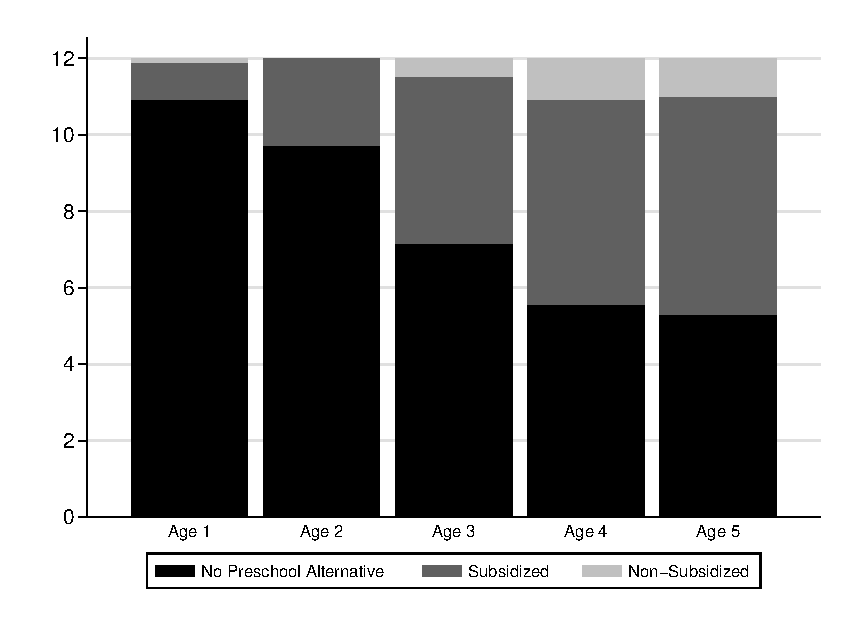
\includegraphics[width=.8\columnwidth]{output/blackwhite_CCnumber.eps}
\floatfoot{
\footnotesize
\noindent Note: This figure describes the take-up of alternative preschool by families in the ABC control group. The vertical axis represents the average number of months per year the subjects of the control group spent in alternative preschool. Subsidized centers were highly regulated and, therefore, relatively high-quality. Non-subsidized childcare services were center-based but not regulated. Other sources of childcare could have included care by parents, relatives, or non-relatives.}
	\end{figure}

	\begin{figure}[H]
		\caption{Average Number of Months in Alternative Preschool, CARE Control and Family Education Groups} \label{fig:cccare}
		\centering
		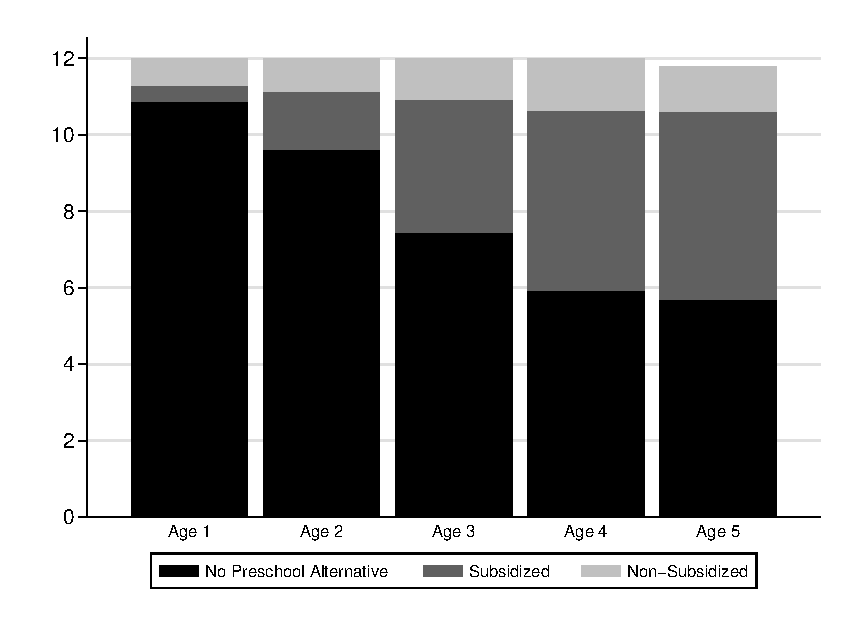
\includegraphics[width=.8\columnwidth]{output/blackwhite_CCnumber_care.eps}
\floatfoot{
\footnotesize
\noindent Note: This figure describes the take-up of alternative preschool by families in the CARE family education and control groups. The vertical axis represents the average number of months per year the subjects of the control group spent in alternative preschool. Subsidized centers were highly regulated and, therefore, relatively high-quality. Non-subsidized childcare services were center-based but not regulated. Other sources of childcare could have included care by parents, relatives, or non-relatives.}
	\end{figure}

\subsubsection{Regulation}

\noindent During the ABC and CARE programs, North Carolina had an active, high-quality system of public childcare for vulnerable families funded by several public programs. Examples include Title IV-A of the Social Service Administration (SSA), Aid to Families with Dependent Children (AFDC), and Title IV-B of Child Welfare Services. These funding efforts were amplified in 1975 by Title XX of the SSA, Social Services Block Grant, which was the main federal source of childcare financing in the US when ABC was active.\footnote{\citet{Robins_1988_Federal-Child-Care}.}\\

\noindent Federally funded childcare services were regulated according to FIDCR standards, which defined stringent regulation for center-based programs for children between the ages of 3 and 6.\footnote{\citet{Department-of-Health_1968_DayCareRequirements}.} These requirements were enforced and childcare providers were aware of them.\footnote{\citet{Kuperman_2015_Clifford-Russell-Interview}.} Additionally, North Carolina had a mandatory licensing law for childcare facilities. This regulation only applied to centers serving children below the age of 3 while FIDCR applied to centers for older children (between the ages of 3 and 6). The relative weakness of this regulation is not very relevant for our study because treatment substitution occurred mostly after age 3.\footnote{\citet{NCGA_1971_House-Bill-100}.} Table~\ref{table:staff} compares a widely-used quality standard, the child-staff ratio, between the North Carolina and FIDCR standards and the actual ABC and CARE numbers.

%Not in main paper
\begin{table}[H]
\caption{Child-Staff Ratios for North Carolina, FIDCR, and Actual ABC and CARE Ratios}
\label{table:staff}
\begin{threeparttable}
\begin{tabular}{lccc}
\toprule
 &NC Standards & FIDCR &  ABC and   \\
Age	& Level I &  Standards  & CARE Ratios\\ \midrule
0--1	& 6:1*	&  				& 	3:1					\\
1--2	& 8:1* 	& 				&   4-5:1				\\
2--3	& 12:1* & 				& 	4-5:1				\\
3--4	& 15:1 	& 		5:1*	& 	4-5:1 				\\
4--5	& 20:1 	& 		7:1*	& 	5-6:1 				\\
5--6 & 25:1  &		7:1*	&	5-6:1				\\
\bottomrule
\end{tabular}
\begin{tablenotes}
\footnotesize
Sources: \cite{Department-of-Health_1968_DayCareRequirements,NCGA_1971_House-Bill-100,Ramey-et-al_1977_Intro-to-ABC,Ramey_Campbell_1979_SR,Ramey_McGinness_etal_1982_Abecedarianapproach, Burchinal_Campbell_etal_1997_CD}.\\
Note: The starred ratios represent the ones we believe were the most relevant for ABC control-group subjects and CARE control-group and family-education-group subjects.
\end{tablenotes}
\end{threeparttable}
\end{table}

\subsubsection{Costs}
% Need citations
\noindent Previous papers have used childcare cost rates that are not specific to North Carolina and do not account for the contemporaneous structure of the subsidies. We use the local subsidy rates that were in place when the ABC subjects were in preschool to impute different costs of the alternative preschools. These costs depend on the specific preschool attended and the eligibility of the families to receive the subsidies. \\

\noindent When ABC was in operation, center-based childcare was subsidized by several federal programs (the Department of Social Services categorized these programs as Child Welfare, AFDC, and Work Incentive Programs).\footnote{\citet{NC-State-Dept_1972_Licensed-Day-Care}.} However, our calculations of the cost of alternative preschool is simplified by the fact that the subsidies were centralized and regulated by the County Department of Social Services. Those departments used a uniform subsidy rate, regardless of the origin of the funds.\footnote{\citet{Ad-Hoc-NC_1974_Letter}.} We collected information about the subsidy rate at the time, which approximates the price of the centers, as centers pegged their fees and services to the maximum subsidy rate. Moreover, we know which centers each ABC control subject attended. We interviewed North Carolina childcare staff and academics that study childcare to document which of those centers were subsidized and regulated at the time.\footnote{\citet{Kuperman_2015_Clifford-Russell-Interview,Kuperman-Hojman_2015_Hodgers-Interview}.} For subsidized centers, we impute the maximum Department of Social Services fee established at the time: \$633/month in 2014 USD.\footnote{\citet{Ad-Hoc-NC_1974_Letter,Comm-Plan-Serv_1973_Durhams-Share}.} For non-subsidized centers, we impute the mean of costs for Level-1 centers (minimum accepted quality level) according to a 1982 North Carolina study of the cost of childcare: \$298/month in 2014 USD.\footnote{\citet{NC-Admin-Branch_1982_Day-Care-Cost-Study}.} Although the information in this survey is not ideal to assess the cost of subsidized preschools, as the subsidies greatly changed after the end of FIDCR (1981), it provides an approximation for assessing the cost of the non-subsidized centers. \\

\noindent Finally, we determine if the families paid the costs themselves or if they were subsidized, in which case we also add deadweight costs. We consider if a subject was eligible for subsidies if the family lived in poverty according to the federal guidelines and all parents living at home worked. If a family is deemed eligible, then we assume the child's preschool was fully subsidized using the rates described above without additional subsidies. \\

\subsection{Data} \label{appendix:data}

In Table~\ref{tab:ecvars_1} through Table~\ref{tab:adultvars_2}, we summarize the data availability for both ABC and CARE. The data collection processes in both programs were analogous by design. For both programs, the treatment and control groups were followed into adulthood with relatively low attrition. For ABC, subjects were followed annually through elementary school and at ages 12, 15, 21, and 30. Health and administrative crime data were collected when the subjects reached their mid-30s. For CARE, the exact same follow-ups are available with the exception of the age 15 follow-up.\\

\begin{sidewaystable}[H]
\small
\caption{Early Childhood Data (Part I)}
\label{tab:ecvars_1}
\centering
\begin{adjustbox}{max width=\textwidth, max height=\textheight,keepaspectratio}
\begin{threeparttable}
\tiny
\begin{tabular}{L{3cm} C{3.5cm} C{4cm} C{1.5cm} C{1.5cm}  C{6cm}}
\toprule
\textbf{Category}	&	\textbf{Sub-Category}	&	\textbf{Description}	&	\textbf{ABC Age}  	&  \textbf{CARE Age}  & 	\textbf{Measure}	\\ \midrule
Demographics	&	Gender	&	Gender of child	&	Birth, 18, 30, 42, 54	&	 Birth, 18, 30, 42, 54	&	Demographic Interview	\\
	&	\\
	&	Race	&	Race/Cultural identity of child	&	Birth, 18, 30, 42, 54	&	 Birth, 18, 30, 42, 54	&	 Demographic Interview\\
	&	\\
	&	Birth Date	&	Date of birth of child	&	Birth, 18, 30, 42, 54	& 	Birth, 18, 30, 42, 54	&	 Demographic Interview	\\ \midrule
Cognitive Assessments	&	Language Ability	&	Auditory association, Verbal expression, etc. 	&	36, 42, 48, 54	&	30, 42, 54	&	ITPA$^{ABC}$, GPB$^{ABC}$, PLP$^{ABC}$, MSCD \\
	&	\\
	&	Intelligence Levels	&	SBIS 	&	24, 36, 48, 60	&	24, 36, 48, 60	&	SBIS	\\
	&		&	WPPSI	&	60	&	60	&	WPPSI	\\
	&		&	BSID 	&	3, 6, 9, 12, 18, 24	&	6, 12, 18, 24		&	BSID	\\
	&		&	UOSPD	&	15	&	- 	&	UOSPD$^{ABC}$	\\
	&		&	RPM	&	60	&	-	&	RPM$^{ABC}$	\\
	&	\\
	&	Quantitative	 &	BSID 	&	3, 6, 9, 12, 18, 24	&	6, 12, 18, 24		&	BSID	\\
	&		&	MSCD 	&	30, 42, 54		&	30, 42, 54	&	MSCD	\\
	&	\\
	&	Memory	&	BSID 	&	3, 6, 9, 12, 18, 24	& 	6, 12, 18, 24		&	BSID	\\
	&		&	MSCD 	&	30, 42, 54	&	30, 42, 54	&	MSCD	\\
	&	\\
	&	Motor Development	&	BSID 	&	3, 6, 9, 12, 18, 24	&	6, 12, 18, 24		&	BSID\\
	&		&	MSCD 	&	30, 42, 54	&	30, 42, 54	&	MSCD	\\
	& 	\\
	&	Critical Thinking	&	Curiosity	&	30, 36, 42, 48, 54, 60, 66, 72	& - &	Infant Behavior Inventory$^{ABC}$	\\ \midrule
Non-Cognitive Assessments	&	Social Skills	&	Positive social response	&	30, 36, 42, 48, 54, 60, 66, 72	&	6, 12, 18, 24		&	Infant Behavior Inventory$^{ABC}$, Bayley Infant Inventory$^{CARE}$	\\
	&		&	Creativity	&	30, 36, 42, 48, 54, 60, 66, 72	&	- 	&	Infant Behavior Inventory$^{ABC}$	\\
	&	\\
	&	Self-Control	&	Locus of control	&	3, 18	&	6, 18	& 	RIES	\\
	&		&	Distractibility, Attentiveness	&	30, 36, 42, 48, 54, 60, 66, 72	&	6, 12, 18, 24		&	Infant Behavior Inventory$^{ABC}$, Bayley Infant Inventory$^{CARE}$	\\
	&	\\
	&	Emotional Health	&	KRT	&	24, 36, 48, 60	&	24, 30, 36, 42, 48, 60	&	KRT	\\
	&	\\
	&	Self-Consciousness	&	Self-consciousness	&	30, 36, 42, 48, 54, 60, 66, 72	&	-	&	Infant Behavior Inventory$^{ABC}$	\\
\bottomrule
\end{tabular}
\begin{tablenotes}
\scriptsize
\item Sources: Authors' description. \\	
\item Note: This table describes the major categories of variables that were measured for ABC and CARE subjects up to age 6. ABC and CARE ages are measured in months. This is not an exhaustive list of variables, nor does it include variables from auxiliary data. Instruments or questionnaires available for only one of the studies are indicated with the superscript $^{ABC}$ or $^{CARE}$.  \textbf{Abbreviations are as follows.} ITPA: Illinois Test of Psycholinguistic Ability. GPB: Gordon Psycholinguistic Battery. PLP: Preschool Language Performance. MSCD: McCarthy Scales of Children's Development. BSID: Bayley Scales of Infant Development and Infant Behavior. UOSPD: Uzgiris-Hunt Ordinal Scales of Psychological Development. RPM: Raven's Progressive Matrices. RIES: Rotter's Internality-Externality Scale. KRT: Kohn and Rosman Test Behavior Inventory.
\end{tablenotes}
\end{threeparttable}
\end{adjustbox}
\end{sidewaystable}




\begin{sidewaystable}[H]
\small
\caption{Early Childhood Data (Part II)}
\label{tab:ecvars_2}
\centering
\begin{adjustbox}{max width=\textwidth, max height=\textheight,keepaspectratio}
\begin{threeparttable}
\tiny
\begin{tabular}{L{3cm} C{3.5cm} C{4cm} C{1.5cm} C{1.5cm}  C{6cm}}
\toprule
\textbf{Category}	&	\textbf{Sub-Category}	&	\textbf{Description}	&	\textbf{ABC Age}  	&  \textbf{CARE Age}  & 	\textbf{Measure}	\\ \midrule
Family Environment	&	Family Members	&	Number of primary caretakers	&	Birth, 18, 30, 42, 54	&	18, 30, 42, 54, 60	&	Demographic Interview	\\
	&		&	Relationship with family members, including father, mother, siblings, etc.	&	Birth, 18, 30, 42, 54	&	18, 30, 42, 54, 60	&	Demographic Interview	\\
	&		&	Number of siblings	&	Birth, 18, 30, 42, 54	&	Birth, 18, 30, 42, 54, 60	&	Demographic Interview	\\
	&		&	Marital status of parents	&	Birth, 18, 30, 42, 54	&	Birth, 18, 30, 42, 54, 60	&	Demographic Interview	\\
	&		&	Marital conflicts between parents	&	6, 18	&	Birth, 6, 18, 36	&	Demographic Interview$^{CARE}$, Parental Attitudes Research Inventory	\\
	&		& Father at home & 18, 30, 42, 54  & 18, 30, 42, 54, 60 & Demographic Interview \\
	&	\\
	&	Family Economic Environment	&	Parents' occupation	&	Birth, 18, 30, 42, 54	& 	Birth, 18, 30, 42, 54, 60		&	Demographic Interview	\\
	&								& Mother works & 18, 30, 42, 54 & 18, 30, 42, 54, 60 & Demographic Interview \\
	&		&	Source of child support	&	Birth, 18, 30, 42, 54	&	18, 30, 42, 54, 60	&	Demographic Interview	\\
	&		&	Family income	&	Birth, 18, 30, 42, 54	&	Birth, 18, 30, 42, 54, 60	&	Demographic Interview	\\
	&	\\
	&	Parents and Home Environment & Parents' authority, warmth, family conflict, etc. & 6, 18, 30, 42, 54 & 6, 12, 18, 30, 42, 54 & Parent Interview \\
	&	\\
	&	Family Social Status	&	Parents' education background	&	Birth, 18, 30, 42, 54	&	Birth, 18, 30, 42, 54, 60		&	Demographic Interview	\\
	&		&	Risk taking of family members	&	Birth	&	- 	&	Parent Interview$^{ABC}$	\\
	&	\\
	&	Family Members' Physical Health	&	Health issues of parents	&	Birth	&	Birth	&	Parent Interview	\\
	&		&	Pregnancy history	&	Birth	&	Birth	&	Parent Interview	\\ \midrule
Childcare	&	Day-care Experience	&	Time and location of day-care, Age when begin	&	Birth, 18, 30, 42, 54	&	18, 30, 42, 54	&	Demographic Interview	\\
			&						& 	Home visits &	-	&	6, 18, 30, 42, 54, 60	& Home Visit Data$^{CARE}$ \\
	&	\\
	&	Parental Care	&	Maternal warmth, Maternal involvement with child	&	6, 18, 30, 42, 54	&	6, 12, 18, 30, 42, 54	&	Home Stimulation	\\
	&		&	Provision of appropriate play materials	&	6, 18, 30, 42, 54	&	 6, 12, 18, 30, 42, 54	&	Home Stimulation	\\
	&		&	Avoidance of restriction and punishment	&	6, 18, 30, 42, 54	&	6, 12, 18, 30		&	Home Stimulation	\\
	&		&	Authoritarian control	&	6, 18, 30, 42, 54	&	6, 12, 18, 30, 36, 42, 102		&	Home Stimulation, Parental Attitudes Research Inventory	\\
	&		&	Democratic attitudes	&	6, 18	&	6, 18, 36	&	Parental Attitudes Research Inventory	\\
	&		&	Hostility and rejection	&	6, 18	&	6, 18, 36	&	Parental Attitudes Research Inventory	\\
	&		&	Parents' knowledge of childcare	&	Birth	&	-	&	Parent Interview$^{ABC}$	\\ \midrule
Physical Health	&	Growth Data	&	Height, Weight, Head circumference, etc.	&	3, 6, 9, 12, 18, 24, 36, 48, 60	&	Birth, 6, 12, 18, 24, 36, 48, 60	&	Growth Measures	\\
\bottomrule
\end{tabular}
\begin{tablenotes}
\scriptsize
\item Sources: Authors' description. \\	
\item Note: This table describes the major categories of variables that were measured for ABC and CARE subjects up to age 6. ABC and CARE ages are measured in months. This is not an exhaustive list of variables, nor does it include variables from auxiliary data.  Instruments or questionnaires available for only one of the studies are indicated with the superscript $^{ABC}$ or $^{CARE}$.
\end{tablenotes}
\end{threeparttable}
\end{adjustbox}
\end{sidewaystable}



\begin{sidewaystable}[H]
\begin{threeparttable}
\small
\caption{Childhood and Adolescence Data (Part I)} \label{tab:youthvars_1}
\centering
\tiny	
\begin{tabular}{L{3.5cm} C{3.5cm} C{5cm} C{1.5cm} C{1.5cm} C{6cm}}
\toprule
\textbf{Category}	&	\textbf{Sub-Category}	&	\textbf{Description}	&	\textbf{ABC Age}  	&  \textbf{CARE Age}  & 	\textbf{Measure}	\\ \midrule
Cognitive Assessment	&	Language Ability	&	Adaptive Language Inventory	&	6, 7, 8	&	6, 7, 8	&	Adaptive Language Inventory	\\
	&		&	Language Questionnaire	&	12	&	- 	&	Language Questionnaire$^{ABC}$	\\
	&		&	MSCD 	&	7	&	- 	&	MSCD$^{ABC}$	\\
	&	\\
	&	Intelligence Tests	&	SBIS	 &	6	&	7	&	SBIS	\\
	&		&	 WIS	&	6, 7, 8, 12, 15	&	6, 8	&	WIS	\\
	&		& Kaufman$^{CARE}$ & 	-	& 6 & Kaufman$^{CARE}$ \\
	&	\\
	&	Quantitative Skills	&	MSCD$^{ABC}$ 	&	7	&	-	&	MSCD$^{ABC}$ 	\\
	&	\\
	&	Memory	&	MSCD$^{ABC}$ 	&	7	&	-	&	MSCD$^{ABC}$	\\
	&	\\
	&	Motor Skills	&	MSCD$^{ABC}$ 	&	7	&	-	&	MSCD$^{ABC}$	\\ \midrule
Non-Cognitive Assessment	&	Interpersonal Skills	&	Gets along with people	&	6, 8, 12, 15	& 	8, 12	&	PEI, CAS, PMI$^{ABC}$, SAI$^{ABC}$, Subject Interview$^{ABC}$, Quality Rank$^{CARE}$	\\
	&		&	Relationship with the other sex	&	15	&	- 	&	 SAI$^{ABC}$, Subject What I Am Like (Harter)$^{ABC}$	\\
	&	\\
	&	Critical Thinking	&	Thinks for self, questions things	&	6, 8	 &	8, 12	&	PEI, Harter Child$^{CARE}$, CBI	\\
	&		&	Concept Attainment Kit	&	6, 7, 8	&	- 	&	Concept Attainment Kit$^{ABC}$	\\
	&	\\
	&	Self-Control	&	Distracted in class	&	6, 7, 8, 12, 15	&	12	&	SCAN$^{ABC}$, CBI, WPB$^{ABC}$, PMI$^{ABC}$, SAI$^{ABC}$, Self-Evaluation Inventory$^{ABC}$	\\
	&		&	Locus of control	&	15	&	- 	&	Nowicki-Strickland Data, Pearlin Mastery Scale$^{ABC}$	\\
	&	\\
	&	Work Ethic	&	Task Orientation	&	6, 7, 8, 12, 15	&	6, 7, 8, 9, 12 	&	SCAN$^{ABC}$, CBI, PMI$^{ABC}$		\\
	&	\\
	&	Emotional Health	&	Harms self, suicidal thoughts	&	8, 12, 15	&	8, 12	 	&	Achenbach Parent,  Subject Risk Taking Survey$^{ABC}$		\\
	&		&	Depression, anxiety, fear, etc.	&	6, 7, 8, 12, 15	&	7, 8, 9, 12	&	KRT, CAS, ETS,  Achenbach Parent	\\
	&	\\
	&	Social Activities	&	Athletic activities	&	8, 12, 15	&	8, 12		&	Achenbach Parent, SAI$^{ABC}$, Subject What I Am Like (Harter)$^{ABC}$, PEI$^{CARE}$	\\
	&		&	Participant of organizations, e.g. religions	&	8, 12, 15	&	8, 12	&	Achenbach Parent, SAI$^{ABC}$, Subject Interview$^{ABC}$	\\
	&		&	Reading list	&	12, 15	&	12	&	CAS, SAI$^{ABC}$	 \\
	&		&	TV/music	&	12, 15	&	12	&	CAS, SAI$^{ABC}$	, Television Checklist$^{ABC}$		\\
	&	\\
	&	Self-Consciousness	&	Self-conscious emotions	&	8, 12, 15	&	8, 12	&	Achenbach Parent, Subject What I Am Like (Harter)	\\ \bottomrule
	\end{tabular}
\begin{tablenotes}
\scriptsize
\item Sources: Authors' descriptions. \\
\item Note: This table describes the major categories of variables that were measured for ABC and CARE subjects at ages 6 to 18. ABC and CARE age are measured in years. This is not an exhaustive list of variables, nor does it include variables from auxiliary data.  Instruments or questionnaires available for only one of the studies are indicated with the superscript $^{ABC}$ or $^{CARE}$. \textbf{Abbreviations are as follows.}  MSCD: McCarthy Scales of Children's Development. SBIS: Stanford-Binet Intelligence Scale. WIS: Wechsler Intelligence Scale for Children. KRT: Kohn and Rosman Test Behavior Inventory. WJCA: Woodcock-Johnson Test of Cognitive Abilities. PEI: Parents as Educator Interview. CAS: Child Assessment Schedule. PMI: Psychosocial Maturity Inventory. SAI: Social Adjustment Inventory for Children and Adolescents. SCAN: Schedule of Classroom Activity Norms. CBI: Classroom Behavior Inventory. WPB: Walker Problem Behavior Checklist. ETS: Emotional/Activity/Sociability/Impulsivity Temperament Survey. FES: Family Environment Scale. PIAT: Peabody Individual Achievement Test. CAT: California Achievement Test. MARS: Mid-Adolescence Rating Scale Data.
\end{tablenotes}
\end{threeparttable}
\end{sidewaystable}

	
	
\begin{sidewaystable}[H]
\begin{threeparttable}
\small
\caption{Childhood and Adolescence Data (Part II)} \label{tab:youthvars_2}
\centering
\tiny
\begin{tabular}{L{3.5cm} C{3.5cm} C{5cm} C{1.5cm} C{1.5cm} C{6cm}}
\toprule
\textbf{Category}	&	\textbf{Sub-Category}	&	\textbf{Description}	&	\textbf{ABC Age}  	&  \textbf{CARE Age}  & 	\textbf{Measure}	\\ \midrule
Family Environment	&	Family Members	&	Number of adults in house	&	6, 8, 12, 15	&	8, 12	&	PEI, Parent Interview, Subject Person In Household$^{ABC}$		\\
	&		&	Relationship with family members, including father, mother, siblings, etc.	&	6, 8, 12, 15	&	8, 12	&	PEI, FES, SAI, Subject Interview$^{ABC}$, Adult Self Report$^{ABC}$, Parent Interview, Achenbach Parent	\\
	&		&	Number of siblings	&	6, 8, 12, 15	&	7, 8, 12	&	PEI$^{ABC}$, Parent Interview	\\
	&		&	Marital status of parents	&	6, 8, 12, 15	&	7, 8, 12	&	PEI$^{ABC}$	, Parent Interview	\\
		&		& Father at home & 18, 30, 42, 54  & 18, 30, 42, 54, 60 & Demographic Interview \\
	&	\\
	&	Parents' Education Style	&	Role of parents in education	&	6, 8	&	8, 12	&	PEI, Parent Interveiw$^{CARE}$	\\
	&		&	Parents' education beliefs \& methods&	6, 8	&	8, 12 	&	PEI, Parent Interview$^{CARE}$		\\
	&		&	Parents' aspiration \& attitudes towards child	&	6, 8, 12, 15	&	8, 12	&	PEI, Parent Interview	\\
	&	\\
	&	Family Economic Environment	&	Parents' occupation	&	6, 8, 12, 15	&	7, 8, 12	&	PEI$^{ABC}$, Parent Interview	\\
		&							& Mother works & 9 & 5, 7, 8 & Demographic Interview \\
	&		&	Source of child support	&	6, 8, 12, 15	&	7, 8, 12	&	PEI$^{ABC}$, Parent Interview	\\
	&		&	Family income	&	6, 8, 12, 15	&	7, 8, 12	&	PEI$^{ABC}$, Parent Interview	\\
	&	\\
		&	Parents and Home Environment & Parents' authority, warmth, family conflict, etc. & 8 & 8 & Parent Interview \\
	&	\\
	&	Family Social Status	&	Parents' education background	&	6, 8, 12, 15	&	7, 8, 12	&	PEI$^{ABC}$, Parent Interview	\\
	&		&	Criminal history and risk taking of family members	&	8, 12, 15	&	- 	&	Subject Taylor Life Events$^{ABC}$, Parent Interview$^{ABC}$	\\
	&	\\
	&	Family Members' Physical Health	&	Health issues of adults in house	&	8, 12, 15	&	12	&	Parent Interview, Subject Taylor Life Events$^{ABC}$	\\ 	\midrule
Academic Achievements	&	Standardized Tests	&	Reading, mathematics, and language abilities	&	6, 7, 8, 12	&	6, 8, 9,12	&	CAT$^{ABC}$, PIAT$^{ABC}$, WJCA	\\
		&	\\
	&	Performance in Schoolwork	&	Drop in grades	&	12, 15		&	12	&	CAS	\\
	&		&	Lack of interest in school	&	12, 15		&	12	&	CAS	\\
	&		&  Total years in special education & 17 & 11 & Retention and Special Services Data \\
	&		&  Total years retained in school & 17 & 11 & Retention and Special Services Data \\  \midrule
Physical Health	&	Health Issues	&	Health issues of subject	&	8, 12, 15	&	8, 12	&	Achenbach Parent, Subject Interview$^{ABC}$, Adult Self Report$^{ABC}$, PEI$^{CARE}$, Parent Interview$^{CARE}$	\\
	&	\\
	&	Growth	&	Vision, weight, height	&	8	&	8	&	Growth Data	\\
	&	\\
	&	Teenage Pregnancy	&	Teenage Pregnancy	&	15	&	- 	& Subject Interview$^{ABC}$		\\ \midrule
Social Conduct	&	Law Breaking	&	Felony, Time spent incarcerated	&	15	&	- 	&	MARS$^{ABC}$, Subject Interview$^{ABC}$	\\ \bottomrule
\end{tabular}
\begin{tablenotes}
\scriptsize
\item Sources: Authors' descriptions. \\
\item Note: This table describes the major categories of variables that were measured for ABC and CARE subjects at ages 6 to 18. ABC and CARE age are measured in years. This is not an exhaustive list of variables, nor does it include variables from auxiliary data.  Instruments or questionnaires available for only one of the studies are indicated with the superscript $^{ABC}$ or $^{CARE}$. \textbf{Abbreviations are as follows.}  MSCD: McCarthy Scales of Children's Development. SBIS: Stanford-Binet Intelligence Scale. WIS: Wechsler Intelligence Scale for Children. KRT: Kohn and Rosman Test Behavior Inventory. WJCA: Woodcock-Johnson Test of Cognitive Abilities. PEI: Parents as Educator Interview. CAS: Child Assessment Schedule. PMI: Psychosocial Maturity Inventory. SAI: Social Adjustment Inventory for Children and Adolescents. SCAN: Schedule of Classroom Activity Norms. CBI: Classroom Behavior Inventory. WPB: Walker Problem Behavior Checklist. ETS: Emotional/Activity/Sociability/Impulsivity Temperament Survey. FES: Family Environment Scale. PIAT: Peabody Individual Achievement Test. CAT: California Achievement Test. MARS: Mid-Adolescence Rating Scale Data.
\end{tablenotes}
\end{threeparttable}
\end{sidewaystable}

\begin{sidewaystable}[H]							
\begin{threeparttable}								
\small										
\caption{Adulthood Data (Part I)} \label{tab:adultvars_1}						\centering										
\scriptsize										
\begin{tabular}{L{3.5cm} C{3.5cm} C{5cm} C{1.5cm} C{1.8cm} C{6cm}}										
\toprule
\textbf{Category}	&	\textbf{Sub-Category}	&	\textbf{Description}	&	\textbf{ABC Age}  	&  \textbf{CARE Age}  & 	\textbf{Measure}	\\ \midrule
Cognitive Assessments   	&	       Intelligence Tests      	&	       WIS     	&	21	&	-	&	       WIS     \\
\midrule										
Non-Cognitive Assessment        	&	       Interpersonal Skills    	&	       Gets along with people  	&	       21, 30  	&	-	&	       Subject Interview   \\
\\										
        	&	       Self-Control    	&	       Locus of control        	&	       21, 30  	&	-	&	       Nowicki-Strickland Data$^{ABC}$, Pearlin Mastery Scale$^{ABC}$  \\
        	&	               	&	       Proud of working, interest in working   	&	       21, 30  	&	21, 30	&	       Job Satisfaction Survey$^{ABC}$, Subject Interview       \\
\\										
        	&	       Emotional Health        	&	       Harms self, suicidal thoughts,	&	21	&	21	&	       Achenbach,  Subject Risk Taking Survey   \\
        	&	               	&	       depression, anxiety, fear, etc. 	&	       21, 30  	&	21, 30	&	       KRT, Achenbach Parent,  CAS, Brief Symptom Inventory, ETS\\
\\										
        	&	       Social Activities       	&	       Athletic activities     	&	21	&	-	&	       Achenbach,  \\
        	&	               	&	       Participant of organizations, e.g. religions    	&	       21, 30  	&	21, 30	&	       Achenbach, Subject Interview        \\
\midrule										
Family Environment      	&	       Family Members  	&	       Number of adults in house       	&	21	&	-	&	       Parent Interview$^{ABC}$ , Subject Interview    \\
        	&	               	&	       Relationship with family members, including father, mother, siblings, etc.      	&	       21, 30  	&	30	&	      Parent Interview, Achenbach$^{ABC}$, Subject Interview, Adult Self Report \\
        	&	               	&	       Number of siblings      	&	       21, 30  	&	30	&	       Parent Interview$^{ABC}$ , Subject Interview    \\
        	&	               	&	       Marital status of parents       	&	21	&	-	&	       Parent Interview$^{ABC}$ , Subject Interview    \\
        	&	               	&	       Number of children, childcare basics    	&	       21, 30  	&	30	&	       Subject Interview, Childcare Questionnaire      \\
\\										
        	&	       Family Economic Environment     	&	       Parents' occupation     	&	21	&	-	&	       Parent Interview$^{ABC}$ , Subject Interview    \\
        	&	               	&	       Source of child support 	&	21	&	30	&	       Parent Interview$^{ABC}$ , Subject Interview    \\
        	&	               	&	       Family income   	&	21	&	30	&	       Parent Interview$^{ABC}$ , Subject Interview    \\
\\										
        	&	       Family Members and Children	&	Relationship quality, family health issues, attitude toward child learning	&	30	&	30	&	       Parent Interview, Taylor Life Events$^{ABC}$, Child Health Questionnaire, PEI    \\
\\										
        	&	       Marital Status  	&	       Marital status, spouse income       	&	       21, 30  	&	21, 30	&	       Subject Interview       \\
        	&	               	&	       Spouse details, marriage history	&	       21, 30  	&	30	&	       Subject Interview       \\
        	&	               	&	       Relationship with spouse        	&	       21, 30  	&	30	&	       Subject Interview, Adult Self Report    \\
\\										
 Achievement   	&	       Education Level 	&	       Years in school, plans for future education      	&	       21, 30  	&	       21, 30  	&	       Subject Interview, Adult Self Report    \\
        	&	               	&	       College type, certificate earned        	&	       21, 30  	&	       21, 30  	&	       Subject Interview, Adult Self Report    \\
	&	Achievement Test	&	       WJCA    	&	       21, 30  	&	-	&	       WJCA    \\
	&		&							
        \\ \bottomrule							
\end{tabular}										
\begin{tablenotes}									
\scriptsize										
\item Sources: Authors' description. \\				
\item Note: This table describes the major categories of variables that were measured for ABC and CARE subjects at ages 21 and 30. ABC and CARE age are measured in years. This is not an exhaustive list of variables, nor does it include variables from auxiliary data. Instruments or questionnaires available for only one of the studies are indicated with the superscript $^{ABC}$ or $^{CARE}$. \textbf{Abbreviations are as follows.} KRT: Kohn and Rosman Test Behavior Inventory. CAS: Child Assessment Schedule. ETS: Emotional/Activity/Sociability/Impulsivity Temperament Survey. WIS: Wechsler Adult Intelligence Scale. WJCA: Woodcock-Johnson Test of Cognitive Abilities. PEI: Parents as Educator Interview.		\end{tablenotes}									
\end{threeparttable}								
\end{sidewaystable}																			


\begin{sidewaystable}[H]
\begin{threeparttable}
\small
\caption{Adulthood Data (Part II)} \label{tab:adultvars_2}
\centering
\scriptsize
\begin{tabular}{L{3.5cm} C{3.5cm} C{5cm} C{1.5cm} C{1.8cm} C{6cm}}
\toprule
\textbf{Category}	&	\textbf{Sub-Category}	&	\textbf{Description}	&	\textbf{ABC Age}  	&  \textbf{CARE Age}  & 	\textbf{Measure}	\\ \midrule
Physical Health	&	Health Insurance	&	Covered by health insurance	&	21, 30	&	21, 30	&	Subject Interview	\\
\\											
	&	Health Issues	&	Health conditions, diseases, regular checkups and tests, mental health	&	21, 30	&	21	&	Brief Symptom Inventory, Subject Interview, Adult Self Report	\\
\midrule											
Social Conduct	&	Risk Taking	&	Smoking, drinking, carry gun, fight, drug use	&	21, 30	&	21, 30	&	Subject Risk Taking Survey, Adult Self Report	\\
\\											
	&	Law Breaking	&	Felony, Time spent incarcerated	&	21	&	21, 30	& Subject Interview	\\
\midrule											
Economic Status	&	Living Circumstances	&	Number of rooms	&	21, 30	&	21, 30	&	Subject Interview	\\
	&		&	Own or rent apartment	&	21, 30	&	21	&	Subject Interview	\\
	&		&	Number living in same domicile	&	21, 30	&	21	&	Subject Interview	\\
\\											
	&	Working Condition	&	Currently employed	&	21, 30	&	21, 30	&	Subject Interview	\\
	&		&	Job title	&	21, 30	&	21, 30	&	Subject Interview, Adult Self Report	\\
	&		&	Job category	&	21, 30	&	21, 30	&	Subject Interview, Adult Self Report	\\
	&		&	Hours	&	21, 30	&	21, 30	&	Subject Interview, Adult Self Report	\\
	&		&	Satisfied with current job	&	21, 30	&	21, 30	&	Subject Interview, Subject What I Am Like (Harter), Adult Self Report	\\
\\											
	&	Transportation	&	Own reliable transportation	&	21, 30	&	21	&	Subject Interview, Adult Self Report	\\
	&		&	Public transportation	&	21, 30	&	21	&	Subject Interview, Adult Self Report	\\
\\											
	&	Income	&	Income from job	&	21, 30	&	21, 30	&	Subject Interview, Adult Self Report	\\
	&		&	Income from welfare programs	&	21, 30	&	30	&	Subject Interview, Adult Self Report	\\
	&		&	Income from investment	&	21, 30	&	-	&	Subject Interview, Adult Self Report	\\										
 \bottomrule
\end{tabular}										
\begin{tablenotes}									
\scriptsize											
\item Sources: Authors' description. \\				
\item Note: This table describes the major categories of variables that were measured for ABC and CARE subjects at ages 21 and 30. ABC and CARE age are measured in years. This is not an exhaustive list of variables, nor does it include variables from auxiliary data. Instruments or questionnaires available for only one of the studies are indicated with the superscript $^{ABC}$ or $^{CARE}$.			
\end{tablenotes}									
\end{threeparttable}								
\end{sidewaystable}											


% AZ: commenting out until we can get the CORRECT numbers in here for both ABC and CARE
\begin{comment}
\begin{figure}[H]
\caption{Attrition by Age, ABC} \label{fig:attrition}
    \centering
  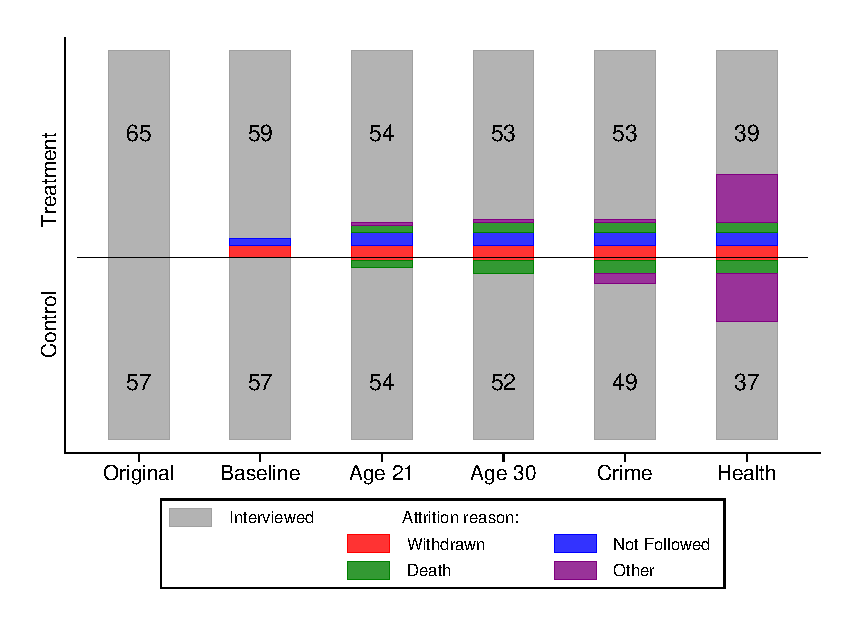
\includegraphics[width=.9\columnwidth]{output/abc_attrition.eps}
  \floatfoot{
\footnotesize
Note: This plot shows the number of participants in ABC for whom there exists data at the periods of data collection by experimental group. The children who withdrew from the study did so due to several reasons, such as adoption. Children were not followed if they were found to be biologically retarded after randomization. The numbers in the bars indicate the number of individuals who were interviewed during that phase of data collection. The original sample was measured after randomization but before the start of the program, the baseline sample was measured at the start of the program, and the health sample was collected at age 34.
}
\end{figure}
\end{comment}

\noindent Attrition was low in ABC. Information is available on 100 subjects in the age 30 follow-up, which we call the adult follow-up. In addition, 80 subjects---40 from the control group and 40 from the treatment group---consented to the release of their criminal records. Further, 70 participants consented to the release of information regarding a full-range biomedical panel---31 from the control group and 39 from the treatment group. \\

\noindent Attrition was also low for CARE subjects. Information is available on 58 subjects (more than 85\% of the initial sample) in the age-30 follow-up. Additionally, 40 participants (11 from the control group, 18 from the family education group, and 11 from the center-based childcare and family education group) released information on the full-range biomedical sweep. Administrative crime data are not available for CARE. We do not evaluate the second-phase of treatment in CARE because it was not randomized. Rather, those in the center-based childcare and family education group and the family education group were offered school-age treatment, and those in the control group were not.  \\ 

\noindent In the following set of tables (Table~\ref{tab:abc_baseline} through Table~\ref{tab:health_baseline}), we compare the observed, baseline characteristics between the first-phase control and treatment groups in ABC, which are the main groups we analyze, at different stages of the data collection follow-ups. For each observed characteristic, we present the bootstrapped $p$-value associated with the standard $t$-test. We also present the bootstrapped, step-down $p$-value on jointly testing the difference in observed characteristics across the two blocks of variables separated by the horizontal line.\footnote{\citet{Lehmann_Romano_2005_testing}.}\\

\noindent First, we compare the first-phase treatment and control groups on baseline characteristics. 

\begin{table}[H]
\captionsetup{singlelinecheck=false,justification=centering}
\caption{First-phase Treatment vs. Control Groups \label{tab:baseline}}

  \begin{threeparttable}
  \begin{tabular}{cccccccc}
  \hline\hline

     &  & \scriptsize{Control} & \scriptsize{Treated} & \scriptsize{Control} & \scriptsize{Treated} & \mc{2}{c}{\scriptsize{$p$-value}} \\  

    \scriptsize{Variable} & \scriptsize{Age} & \scriptsize{Obs.} & \scriptsize{Obs.} & \scriptsize{Mean} & \scriptsize{Mean} & \scriptsize{Single $H_0$} & \scriptsize{Multiple $H_0$} \\ 
    \hline  

    \mc{1}{l}{\scriptsize{Male}} & \mc{1}{c}{\scriptsize{0}} & \mc{1}{c}{\scriptsize{57}} & \mc{1}{c}{\scriptsize{59}} & \mc{1}{c}{\scriptsize{0.438}} & \mc{1}{c}{\scriptsize{0.489}} & \mc{1}{c}{\scriptsize{(0.580)}} & \mc{1}{c}{\scriptsize{(0.700)}} \\  

    \mc{1}{l}{\scriptsize{Birth Weight}} & \mc{1}{c}{\scriptsize{0}} & \mc{1}{c}{\scriptsize{56}} & \mc{1}{c}{\scriptsize{58}} & \mc{1}{c}{\scriptsize{7.191}} & \mc{1}{c}{\scriptsize{6.829}} & \mc{1}{c}{\scriptsize{(0.130)}} & \mc{1}{c}{\scriptsize{(0.205)}} \\  

    \mc{1}{l}{\scriptsize{No. Siblings in Household}} & \mc{1}{c}{\scriptsize{0}} & \mc{1}{c}{\scriptsize{57}} & \mc{1}{c}{\scriptsize{59}} & \mc{1}{c}{\scriptsize{0.750}} & \mc{1}{c}{\scriptsize{0.516}} & \mc{1}{c}{\scriptsize{(0.245)}} & \mc{1}{c}{\scriptsize{(0.425)}} \\  

    \mc{1}{l}{\scriptsize{Birth Year}} & \mc{1}{c}{\scriptsize{0}} & \mc{1}{c}{\scriptsize{57}} & \mc{1}{c}{\scriptsize{59}} & \mc{1}{c}{\scriptsize{1974}} & \mc{1}{c}{\scriptsize{1974}} & \mc{1}{c}{\scriptsize{(0.785)}} & \mc{1}{c}{\scriptsize{(0.865)}} \\ 
    \hline  

    \mc{1}{l}{\scriptsize{Mother's Education}} & \mc{1}{c}{\scriptsize{0}} & \mc{1}{c}{\scriptsize{57}} & \mc{1}{c}{\scriptsize{59}} & \mc{1}{c}{\scriptsize{9.864}} & \mc{1}{c}{\scriptsize{10.505}} & \mc{1}{c}{\scriptsize{\textbf{(0.050)}}} & \mc{1}{c}{\scriptsize{\textbf{(0.090)}}} \\  

    \mc{1}{l}{\scriptsize{Mother's Age}} & \mc{1}{c}{\scriptsize{0}} & \mc{1}{c}{\scriptsize{57}} & \mc{1}{c}{\scriptsize{59}} & \mc{1}{c}{\scriptsize{20.103}} & \mc{1}{c}{\scriptsize{19.564}} & \mc{1}{c}{\scriptsize{(0.555)}} & \mc{1}{c}{\scriptsize{(0.665)}} \\  

    \mc{1}{l}{\scriptsize{Parental Income}} & \mc{1}{c}{\scriptsize{0}} & \mc{1}{c}{\scriptsize{57}} & \mc{1}{c}{\scriptsize{58}} & \mc{1}{c}{\scriptsize{6,211}} & \mc{1}{c}{\scriptsize{7,019}} & \mc{1}{c}{\scriptsize{(0.645)}} & \mc{1}{c}{\scriptsize{(0.720)}} \\  

    \mc{1}{l}{\scriptsize{Mother's IQ}} & \mc{1}{c}{\scriptsize{0}} & \mc{1}{c}{\scriptsize{57}} & \mc{1}{c}{\scriptsize{59}} & \mc{1}{c}{\scriptsize{83.419}} & \mc{1}{c}{\scriptsize{85.393}} & \mc{1}{c}{\scriptsize{(0.360)}} & \mc{1}{c}{\scriptsize{(0.510)}} \\  

    \mc{1}{l}{\scriptsize{Father at Home}} & \mc{1}{c}{\scriptsize{0}} & \mc{1}{c}{\scriptsize{57}} & \mc{1}{c}{\scriptsize{59}} & \mc{1}{c}{\scriptsize{0.346}} & \mc{1}{c}{\scriptsize{0.223}} & \mc{1}{c}{\scriptsize{(0.135)}} & \mc{1}{c}{\scriptsize{(0.270)}} \\  

  \hline\hline
  \end{tabular}
    \begin{tablenotes}
    \scriptsize
    \item 
    Note: This table shows the balance in observed characteristics between the treatment and control groups at baseline.
    For each characteristic, we present the $p$-value from a single hypothesis test.
    We also present the $p$-values from multiple testing, where we collectively test the
    baseline characteristics within the blocks separated by the horizontal line.
    Both $p$-values are two-sided and non-parametric. We construct them 
    based on 1,000 re-draws of the full sample. The estimates we display are the means of 
    the empirical bootstrap distribution. 
    
    \end{tablenotes}
  \end{threeparttable}

\end{table}

\noindent Second, we present the same exercise for each of the four cohorts ABC served.

\begin{table}[H]
\captionsetup{singlelinecheck=false,justification=centering}
\caption{First-phase Treatment vs. Control Groups, ABC Cohort 1 \label{tab:baseline_coh1}}

  \begin{threeparttable}
  \begin{tabular}{cccccccc}
  \toprule

     &  & \scriptsize{Control} & \scriptsize{Treated} & \scriptsize{Control} & \scriptsize{Treated} & \mc{2}{c}{\scriptsize{$p$-value}} \\  

    \scriptsize{Variable} & \scriptsize{Age} & \scriptsize{Obs.} & \scriptsize{Obs.} & \scriptsize{Mean} & \scriptsize{Mean} & \scriptsize{Single $H_0$} & \scriptsize{Multiple $H_0$} \\ 
    \midrule  

    \mc{1}{l}{\scriptsize{Male}} & \mc{1}{c}{\scriptsize{0}} & \mc{1}{c}{\scriptsize{14}} & \mc{1}{c}{\scriptsize{14}} & \mc{1}{c}{\scriptsize{0.348}} & \mc{1}{c}{\scriptsize{0.286}} & \mc{1}{c}{\scriptsize{(0.730)}} & \mc{1}{c}{\scriptsize{(0.738)}} \\  

    \mc{1}{l}{\scriptsize{Birth Weight}} & \mc{1}{c}{\scriptsize{0}} & \mc{1}{c}{\scriptsize{14}} & \mc{1}{c}{\scriptsize{13}} & \mc{1}{c}{\scriptsize{6.755}} & \mc{1}{c}{\scriptsize{6.491}} & \mc{1}{c}{\scriptsize{(0.550)}} & \mc{1}{c}{\scriptsize{(0.655)}} \\  

    \mc{1}{l}{\scriptsize{No. Siblings in Household}} & \mc{1}{c}{\scriptsize{0}} & \mc{1}{c}{\scriptsize{14}} & \mc{1}{c}{\scriptsize{14}} & \mc{1}{c}{\scriptsize{1.741}} & \mc{1}{c}{\scriptsize{0.606}} & \mc{1}{c}{\scriptsize{\textbf{(0.035)}}} & \mc{1}{c}{\scriptsize{\textbf{(0.085)}}} \\  

    \mc{1}{l}{\scriptsize{Birth Year}} & \mc{1}{c}{\scriptsize{0}} & \mc{1}{c}{\scriptsize{14}} & \mc{1}{c}{\scriptsize{14}} & \mc{1}{c}{\scriptsize{1972}} & \mc{1}{c}{\scriptsize{1972}} & \mc{1}{c}{\scriptsize{(0.240)}} & \mc{1}{c}{\scriptsize{(0.350)}} \\ 
    \midrule 

    \mc{1}{l}{\scriptsize{Mother's Education}} & \mc{1}{c}{\scriptsize{0}} & \mc{1}{c}{\scriptsize{14}} & \mc{1}{c}{\scriptsize{14}} & \mc{1}{c}{\scriptsize{9.885}} & \mc{1}{c}{\scriptsize{10.561}} & \mc{1}{c}{\scriptsize{(0.265)}} & \mc{1}{c}{\scriptsize{(0.480)}} \\  

    \mc{1}{l}{\scriptsize{Mother's Age}} & \mc{1}{c}{\scriptsize{0}} & \mc{1}{c}{\scriptsize{14}} & \mc{1}{c}{\scriptsize{14}} & \mc{1}{c}{\scriptsize{23.869}} & \mc{1}{c}{\scriptsize{19.552}} & \mc{1}{c}{\scriptsize{\textbf{(0.050)}}} & \mc{1}{c}{\scriptsize{(0.135)}} \\  

    \mc{1}{l}{\scriptsize{Mother Employed}} & \mc{1}{c}{\scriptsize{0}} & \mc{1}{c}{\scriptsize{14}} & \mc{1}{c}{\scriptsize{14}} & \mc{1}{c}{\scriptsize{0.152}} & \mc{1}{c}{\scriptsize{0.205}} & \mc{1}{c}{\scriptsize{(0.695)}} & \mc{1}{c}{\scriptsize{(0.895)}} \\  

    \mc{1}{l}{\scriptsize{Parental Income}} & \mc{1}{c}{\scriptsize{0}} & \mc{1}{c}{\scriptsize{14}} & \mc{1}{c}{\scriptsize{13}} & \mc{1}{c}{\scriptsize{7,164}} & \mc{1}{c}{\scriptsize{8,298}} & \mc{1}{c}{\scriptsize{(0.755)}} & \mc{1}{c}{\scriptsize{(0.910)}} \\  

    \mc{1}{l}{\scriptsize{Mother's IQ}} & \mc{1}{c}{\scriptsize{0}} & \mc{1}{c}{\scriptsize{14}} & \mc{1}{c}{\scriptsize{14}} & \mc{1}{c}{\scriptsize{76.042}} & \mc{1}{c}{\scriptsize{81.108}} & \mc{1}{c}{\scriptsize{(0.270)}} & \mc{1}{c}{\scriptsize{(0.485)}} \\  

    \mc{1}{l}{\scriptsize{Father at Home}} & \mc{1}{c}{\scriptsize{0}} & \mc{1}{c}{\scriptsize{14}} & \mc{1}{c}{\scriptsize{14}} & \mc{1}{c}{\scriptsize{0.559}} & \mc{1}{c}{\scriptsize{0.368}} & \mc{1}{c}{\scriptsize{(0.340)}} & \mc{1}{c}{\scriptsize{(0.493)}} \\  

  \bottomrule
  \end{tabular}
    \begin{tablenotes}
    \scriptsize
    \item 
    Note: This table shows the balance in observed characteristics between the treatment and control groups in ABC at baseline for cohort 1.
    For each characteristic, we present the $p$-value from a single hypothesis test.
    We also present the $p$-values from multiple hypothesis testing, where we collectively test the
    baseline characteristics within the blocks separated by the horizontal line.
    Both $p$-values are two-sided and non-parametric. We construct them 
    based on 200 re-draws of the full sample.
    
    \end{tablenotes}
  \end{threeparttable}

\end{table}

\begin{table}[H]
\captionsetup{singlelinecheck=false,justification=centering}
\caption{First-phase Treatment vs. Control Groups, ABC Cohort 2 \label{tab:baseline_coh2}}

  \begin{threeparttable}
  \begin{tabular}{cccccccc}
  \toprule

     &  & \scriptsize{Control} & \scriptsize{Treated} & \scriptsize{Control} & \scriptsize{Treated} & \mc{2}{c}{\scriptsize{$p$-value}} \\  

    \scriptsize{Variable} & \scriptsize{Age} & \scriptsize{Obs.} & \scriptsize{Obs.} & \scriptsize{Mean} & \scriptsize{Mean} & \scriptsize{Single $H_0$} & \scriptsize{Multiple $H_0$} \\ 
    \midrule

    \mc{1}{l}{\scriptsize{Male}} & \mc{1}{c}{\scriptsize{0}} & \mc{1}{c}{\scriptsize{13}} & \mc{1}{c}{\scriptsize{16}} & \mc{1}{c}{\scriptsize{0.457}} & \mc{1}{c}{\scriptsize{0.503}} & \mc{1}{c}{\scriptsize{(0.805)}} & \mc{1}{c}{\scriptsize{(0.875)}} \\  

    \mc{1}{l}{\scriptsize{Birth Weight}} & \mc{1}{c}{\scriptsize{0}} & \mc{1}{c}{\scriptsize{13}} & \mc{1}{c}{\scriptsize{16}} & \mc{1}{c}{\scriptsize{7.256}} & \mc{1}{c}{\scriptsize{6.534}} & \mc{1}{c}{\scriptsize{(0.160)}} & \mc{1}{c}{\scriptsize{(0.270)}} \\  

    \mc{1}{l}{\scriptsize{No. Siblings in Household}} & \mc{1}{c}{\scriptsize{0}} & \mc{1}{c}{\scriptsize{13}} & \mc{1}{c}{\scriptsize{16}} & \mc{1}{c}{\scriptsize{0.388}} & \mc{1}{c}{\scriptsize{0.316}} & \mc{1}{c}{\scriptsize{(0.755)}} & \mc{1}{c}{\scriptsize{(0.835)}} \\  

    \mc{1}{l}{\scriptsize{Birth Year}} & \mc{1}{c}{\scriptsize{0}} & \mc{1}{c}{\scriptsize{13}} & \mc{1}{c}{\scriptsize{16}} & \mc{1}{c}{\scriptsize{1973}} & \mc{1}{c}{\scriptsize{1973}} & \mc{1}{c}{\scriptsize{(0.850)}} & \mc{1}{c}{\scriptsize{(0.925)}} \\ 
    \midrule  

    \mc{1}{l}{\scriptsize{Mother's Education}} & \mc{1}{c}{\scriptsize{0}} & \mc{1}{c}{\scriptsize{13}} & \mc{1}{c}{\scriptsize{16}} & \mc{1}{c}{\scriptsize{10.225}} & \mc{1}{c}{\scriptsize{10.307}} & \mc{1}{c}{\scriptsize{(0.885)}} & \mc{1}{c}{\scriptsize{(0.940)}} \\  

    \mc{1}{l}{\scriptsize{Mother's Age}} & \mc{1}{c}{\scriptsize{0}} & \mc{1}{c}{\scriptsize{13}} & \mc{1}{c}{\scriptsize{16}} & \mc{1}{c}{\scriptsize{18.446}} & \mc{1}{c}{\scriptsize{17.637}} & \mc{1}{c}{\scriptsize{(0.380)}} & \mc{1}{c}{\scriptsize{(0.630)}} \\  

    \mc{1}{l}{\scriptsize{Mother Employed}} & \mc{1}{c}{\scriptsize{0}} & \mc{1}{c}{\scriptsize{13}} & \mc{1}{c}{\scriptsize{16}} & \mc{1}{c}{\scriptsize{0.307}} & \mc{1}{c}{\scriptsize{0.248}} & \mc{1}{c}{\scriptsize{(0.690)}} & \mc{1}{c}{\scriptsize{(0.850)}} \\  

    \mc{1}{l}{\scriptsize{Parental Income}} & \mc{1}{c}{\scriptsize{0}} & \mc{1}{c}{\scriptsize{13}} & \mc{1}{c}{\scriptsize{16}} & \mc{1}{c}{\scriptsize{5,398}} & \mc{1}{c}{\scriptsize{4,427}} & \mc{1}{c}{\scriptsize{(0.790)}} & \mc{1}{c}{\scriptsize{(0.880)}} \\  

    \mc{1}{l}{\scriptsize{Mother's IQ}} & \mc{1}{c}{\scriptsize{0}} & \mc{1}{c}{\scriptsize{13}} & \mc{1}{c}{\scriptsize{16}} & \mc{1}{c}{\scriptsize{86.873}} & \mc{1}{c}{\scriptsize{85.597}} & \mc{1}{c}{\scriptsize{(0.730)}} & \mc{1}{c}{\scriptsize{(0.855)}} \\  

    \mc{1}{l}{\scriptsize{Father at Home}} & \mc{1}{c}{\scriptsize{0}} & \mc{1}{c}{\scriptsize{13}} & \mc{1}{c}{\scriptsize{16}} & \mc{1}{c}{\scriptsize{0.220}} & \mc{1}{c}{\scriptsize{0.183}} & \mc{1}{c}{\scriptsize{(0.790)}} & \mc{1}{c}{\scriptsize{(0.895)}} \\  

  \bottomrule
  \end{tabular}
    \begin{tablenotes}
    \scriptsize
    \item 
    Note: This table shows the balance in observed characteristics between the treatment and control groups in ABC at baseline for cohort 2.
    For each characteristic, we present the $p$-value from a single hypothesis test.
    We also present the $p$-values from multiple hypothesis testing, where we collectively test the
    baseline characteristics within the blocks separated by the horizontal line.
    Both $p$-values are two-sided and non-parametric. We construct them 
    based on 200 re-draws of the full sample.
    
    \end{tablenotes}
  \end{threeparttable}

\end{table}

\begin{table}[H]
\captionsetup{singlelinecheck=false,justification=centering}
\caption{First-phase Treatment vs. Control Groups, ABC Cohort 3 \label{tab:baseline_coh3}}

  \begin{threeparttable}
  \begin{tabular}{cccccccc}
  \hline\hline

     &  & \scriptsize{Control} & \scriptsize{Treated} & \scriptsize{Control} & \scriptsize{Treated} & \mc{2}{c}{\scriptsize{$p$-value}} \\  

    \scriptsize{Variable} & \scriptsize{Age} & \scriptsize{Obs.} & \scriptsize{Obs.} & \scriptsize{Mean} & \scriptsize{Mean} & \scriptsize{Single $H_0$} & \scriptsize{Multiple $H_0$} \\ 
    \hline  

    \mc{1}{l}{\scriptsize{Male}} & \mc{1}{c}{\scriptsize{0}} & \mc{1}{c}{\scriptsize{14}} & \mc{1}{c}{\scriptsize{15}} & \mc{1}{c}{\scriptsize{0.376}} & \mc{1}{c}{\scriptsize{0.596}} & \mc{1}{c}{\scriptsize{(0.265)}} & \mc{1}{c}{\scriptsize{(0.320)}} \\  

    \mc{1}{l}{\scriptsize{Birth Weight}} & \mc{1}{c}{\scriptsize{0}} & \mc{1}{c}{\scriptsize{14}} & \mc{1}{c}{\scriptsize{15}} & \mc{1}{c}{\scriptsize{7.424}} & \mc{1}{c}{\scriptsize{7.138}} & \mc{1}{c}{\scriptsize{(0.470)}} & \mc{1}{c}{\scriptsize{(0.730)}} \\  

    \mc{1}{l}{\scriptsize{No. Siblings in Household}} & \mc{1}{c}{\scriptsize{0}} & \mc{1}{c}{\scriptsize{14}} & \mc{1}{c}{\scriptsize{15}} & \mc{1}{c}{\scriptsize{0.423}} & \mc{1}{c}{\scriptsize{0.203}} & \mc{1}{c}{\scriptsize{(0.385)}} & \mc{1}{c}{\scriptsize{(0.645)}} \\  

    \mc{1}{l}{\scriptsize{Birth Year}} & \mc{1}{c}{\scriptsize{0}} & \mc{1}{c}{\scriptsize{14}} & \mc{1}{c}{\scriptsize{15}} & \mc{1}{c}{\scriptsize{1975}} & \mc{1}{c}{\scriptsize{1975}} & \mc{1}{c}{\scriptsize{(0.510)}} & \mc{1}{c}{\scriptsize{(0.520)}} \\ 
    \hline  

    \mc{1}{l}{\scriptsize{Mother's Education}} & \mc{1}{c}{\scriptsize{0}} & \mc{1}{c}{\scriptsize{14}} & \mc{1}{c}{\scriptsize{15}} & \mc{1}{c}{\scriptsize{10.133}} & \mc{1}{c}{\scriptsize{10.704}} & \mc{1}{c}{\scriptsize{(0.405)}} & \mc{1}{c}{\scriptsize{(0.595)}} \\  

    \mc{1}{l}{\scriptsize{Mother's Age}} & \mc{1}{c}{\scriptsize{0}} & \mc{1}{c}{\scriptsize{14}} & \mc{1}{c}{\scriptsize{15}} & \mc{1}{c}{\scriptsize{18.602}} & \mc{1}{c}{\scriptsize{19.558}} & \mc{1}{c}{\scriptsize{(0.355)}} & \mc{1}{c}{\scriptsize{(0.570)}} \\  

    \mc{1}{l}{\scriptsize{Mother Employed}} & \mc{1}{c}{\scriptsize{0}} & \mc{1}{c}{\scriptsize{14}} & \mc{1}{c}{\scriptsize{15}} & \mc{1}{c}{\scriptsize{0.162}} & \mc{1}{c}{\scriptsize{0.467}} & \mc{1}{c}{\scriptsize{\textbf{(0.070)}}} & \mc{1}{c}{\scriptsize{(0.155)}} \\  

    \mc{1}{l}{\scriptsize{Parental Income}} & \mc{1}{c}{\scriptsize{0}} & \mc{1}{c}{\scriptsize{14}} & \mc{1}{c}{\scriptsize{15}} & \mc{1}{c}{\scriptsize{7,034}} & \mc{1}{c}{\scriptsize{4,981}} & \mc{1}{c}{\scriptsize{(0.430)}} & \mc{1}{c}{\scriptsize{(0.675)}} \\  

    \mc{1}{l}{\scriptsize{Mother's IQ}} & \mc{1}{c}{\scriptsize{0}} & \mc{1}{c}{\scriptsize{14}} & \mc{1}{c}{\scriptsize{15}} & \mc{1}{c}{\scriptsize{85.590}} & \mc{1}{c}{\scriptsize{88.715}} & \mc{1}{c}{\scriptsize{(0.435)}} & \mc{1}{c}{\scriptsize{(0.610)}} \\  

    \mc{1}{l}{\scriptsize{Father at Home}} & \mc{1}{c}{\scriptsize{0}} & \mc{1}{c}{\scriptsize{14}} & \mc{1}{c}{\scriptsize{15}} & \mc{1}{c}{\scriptsize{0.424}} & \mc{1}{c}{\scriptsize{0.209}} & \mc{1}{c}{\scriptsize{(0.265)}} & \mc{1}{c}{\scriptsize{(0.425)}} \\  

  \hline\hline
  \end{tabular}
    \begin{tablenotes}
    \scriptsize
    \item 
    Note: This table shows the balance in observed characteristics between the treatment and control groups in ABC at baseline for cohort 3.
    For each characteristic, we present the $p$-value from a single hypothesis test.
    We also present the $p$-values from multiple testing, where we collectively test the
    baseline characteristics within the blocks separated by the horizontal line.
    Both $p$-values are two-sided and non-parametric. We construct them 
    based on 200 re-draws of the full sample. The estimates we display are the means of 
    the empirical bootstrap distribution. 
    
    \end{tablenotes}
  \end{threeparttable}

\end{table}

\begin{table}[H]
\captionsetup{singlelinecheck=false,justification=centering}
\caption{First-phase Treatment vs. Control Groups, ABC Cohort 4 \label{tab:baseline_coh4}}

  \begin{threeparttable}
  \begin{tabular}{cccccccc}
  \toprule

     &  & \scriptsize{Control} & \scriptsize{Treated} & \scriptsize{Control} & \scriptsize{Treated} & \mc{2}{c}{\scriptsize{$p$-value}} \\  

    \scriptsize{Variable} & \scriptsize{Age} & \scriptsize{Obs.} & \scriptsize{Obs.} & \scriptsize{Mean} & \scriptsize{Mean} & \scriptsize{Single $H_0$} & \scriptsize{Multiple $H_0$} \\ 
    \midrule

    \mc{1}{l}{\scriptsize{Male}} & \mc{1}{c}{\scriptsize{0}} & \mc{1}{c}{\scriptsize{15}} & \mc{1}{c}{\scriptsize{14}} & \mc{1}{c}{\scriptsize{0.599}} & \mc{1}{c}{\scriptsize{0.567}} & \mc{1}{c}{\scriptsize{(0.870)}} & \mc{1}{c}{\scriptsize{(0.905)}} \\  

    \mc{1}{l}{\scriptsize{Birth Weight}} & \mc{1}{c}{\scriptsize{0}} & \mc{1}{c}{\scriptsize{15}} & \mc{1}{c}{\scriptsize{14}} & \mc{1}{c}{\scriptsize{7.321}} & \mc{1}{c}{\scriptsize{7.150}} & \mc{1}{c}{\scriptsize{(0.725)}} & \mc{1}{c}{\scriptsize{(0.840)}} \\  

    \mc{1}{l}{\scriptsize{No. Siblings in Household}} & \mc{1}{c}{\scriptsize{0}} & \mc{1}{c}{\scriptsize{15}} & \mc{1}{c}{\scriptsize{14}} & \mc{1}{c}{\scriptsize{0.490}} & \mc{1}{c}{\scriptsize{0.977}} & \mc{1}{c}{\scriptsize{(0.220)}} & \mc{1}{c}{\scriptsize{(0.380)}} \\  

    \mc{1}{l}{\scriptsize{Birth Year}} & \mc{1}{c}{\scriptsize{0}} & \mc{1}{c}{\scriptsize{15}} & \mc{1}{c}{\scriptsize{14}} & \mc{1}{c}{\scriptsize{1977}} & \mc{1}{c}{\scriptsize{1977}} & \mc{1}{c}{\scriptsize{(0.615)}} & \mc{1}{c}{\scriptsize{(0.728)}} \\ 
    \midrule

    \mc{1}{l}{\scriptsize{Mother's Education}} & \mc{1}{c}{\scriptsize{0}} & \mc{1}{c}{\scriptsize{15}} & \mc{1}{c}{\scriptsize{14}} & \mc{1}{c}{\scriptsize{9.530}} & \mc{1}{c}{\scriptsize{10.424}} & \mc{1}{c}{\scriptsize{(0.240)}} & \mc{1}{c}{\scriptsize{(0.410)}} \\  

    \mc{1}{l}{\scriptsize{Mother's Age}} & \mc{1}{c}{\scriptsize{0}} & \mc{1}{c}{\scriptsize{15}} & \mc{1}{c}{\scriptsize{14}} & \mc{1}{c}{\scriptsize{19.941}} & \mc{1}{c}{\scriptsize{21.712}} & \mc{1}{c}{\scriptsize{(0.320)}} & \mc{1}{c}{\scriptsize{(0.570)}} \\  

    \mc{1}{l}{\scriptsize{Mother Employed}} & \mc{1}{c}{\scriptsize{0}} & \mc{1}{c}{\scriptsize{15}} & \mc{1}{c}{\scriptsize{14}} & \mc{1}{c}{\scriptsize{0.260}} & \mc{1}{c}{\scriptsize{0.347}} & \mc{1}{c}{\scriptsize{(0.650)}} & \mc{1}{c}{\scriptsize{(0.840)}} \\  

    \mc{1}{l}{\scriptsize{Parental Income}} & \mc{1}{c}{\scriptsize{0}} & \mc{1}{c}{\scriptsize{15}} & \mc{1}{c}{\scriptsize{14}} & \mc{1}{c}{\scriptsize{5,827}} & \mc{1}{c}{\scriptsize{10,781}} & \mc{1}{c}{\scriptsize{\textbf{(0.065)}}} & \mc{1}{c}{\scriptsize{(0.135)}} \\  

    \mc{1}{l}{\scriptsize{Mother's IQ}} & \mc{1}{c}{\scriptsize{0}} & \mc{1}{c}{\scriptsize{15}} & \mc{1}{c}{\scriptsize{14}} & \mc{1}{c}{\scriptsize{85.561}} & \mc{1}{c}{\scriptsize{86.004}} & \mc{1}{c}{\scriptsize{(0.920)}} & \mc{1}{c}{\scriptsize{(0.960)}} \\  

    \mc{1}{l}{\scriptsize{Father at Home}} & \mc{1}{c}{\scriptsize{0}} & \mc{1}{c}{\scriptsize{15}} & \mc{1}{c}{\scriptsize{14}} & \mc{1}{c}{\scriptsize{0.208}} & \mc{1}{c}{\scriptsize{0.138}} & \mc{1}{c}{\scriptsize{(0.570)}} & \mc{1}{c}{\scriptsize{(0.777)}} \\  

  \bottomrule
  \end{tabular}
    \begin{tablenotes}
    \scriptsize
    \item 
    Note: This table shows the balance in observed characteristics between the treatment and control groups in ABC at baseline for cohort 4.
    For each characteristic, we present the $p$-value from a single hypothesis test.
    We also present the $p$-values from multiple hypothesis testing, where we collectively test the
    baseline characteristics within the blocks separated by the horizontal line.
    Both $p$-values are two-sided and non-parametric. We construct them 
    based on 200 re-draws of the full sample. The estimates we display are the means of 
    the empirical bootstrap distribution. 
    
    \end{tablenotes}
  \end{threeparttable}

\end{table}

\noindent Third, we compare the second-phase treatment and control groups on baseline characteristics. 

\begin{table}[H]
\captionsetup{singlelinecheck=false,justification=centering}
\caption{Second-phase Treatment vs. Control Groups \label{tab:baseline_sa}}

  \begin{threeparttable}
  \begin{tabular}{cccccccc}
  \hline\hline

     &  & \scriptsize{Control} & \scriptsize{Treatment} & \scriptsize{Control} & \scriptsize{Treated} & \mc{2}{c}{\scriptsize{$p$-value}} \\  

    \scriptsize{Variable} & \scriptsize{Age} & \scriptsize{Obs.} & \scriptsize{Obs.} & \scriptsize{Mean} & \scriptsize{Mean} & \scriptsize{Single $H_0$} & \scriptsize{Multiple $H_0$} \\ 
    \hline  

    \mc{1}{l}{\scriptsize{Male}} & \mc{1}{c}{\scriptsize{0}} & \mc{1}{c}{\scriptsize{47}} & \mc{1}{c}{\scriptsize{48}} & \mc{1}{c}{\scriptsize{0.551}} & \mc{1}{c}{\scriptsize{0.460}} & \mc{1}{c}{\scriptsize{(0.420)}} & \mc{1}{c}{\scriptsize{(0.552)}} \\  

    \mc{1}{l}{\scriptsize{Birth Weight}} & \mc{1}{c}{\scriptsize{0}} & \mc{1}{c}{\scriptsize{47}} & \mc{1}{c}{\scriptsize{48}} & \mc{1}{c}{\scriptsize{7.084}} & \mc{1}{c}{\scriptsize{6.929}} & \mc{1}{c}{\scriptsize{(0.610)}} & \mc{1}{c}{\scriptsize{(0.700)}} \\  

    \mc{1}{l}{\scriptsize{No. Siblings in Household}} & \mc{1}{c}{\scriptsize{0}} & \mc{1}{c}{\scriptsize{47}} & \mc{1}{c}{\scriptsize{48}} & \mc{1}{c}{\scriptsize{0.748}} & \mc{1}{c}{\scriptsize{0.504}} & \mc{1}{c}{\scriptsize{(0.285)}} & \mc{1}{c}{\scriptsize{(0.445)}} \\  

    \mc{1}{l}{\scriptsize{Birth Year}} & \mc{1}{c}{\scriptsize{0}} & \mc{1}{c}{\scriptsize{47}} & \mc{1}{c}{\scriptsize{48}} & \mc{1}{c}{\scriptsize{1974}} & \mc{1}{c}{\scriptsize{1974}} & \mc{1}{c}{\scriptsize{(0.835)}} & \mc{1}{c}{\scriptsize{(0.915)}} \\ 
    \hline  

    \mc{1}{l}{\scriptsize{Mother's Education}} & \mc{1}{c}{\scriptsize{0}} & \mc{1}{c}{\scriptsize{47}} & \mc{1}{c}{\scriptsize{48}} & \mc{1}{c}{\scriptsize{10.150}} & \mc{1}{c}{\scriptsize{10.388}} & \mc{1}{c}{\scriptsize{(0.480)}} & \mc{1}{c}{\scriptsize{(0.685)}} \\  

    \mc{1}{l}{\scriptsize{Mother's Age}} & \mc{1}{c}{\scriptsize{0}} & \mc{1}{c}{\scriptsize{47}} & \mc{1}{c}{\scriptsize{48}} & \mc{1}{c}{\scriptsize{21.122}} & \mc{1}{c}{\scriptsize{18.884}} & \mc{1}{c}{\scriptsize{\textbf{(0.035)}}} & \mc{1}{c}{\scriptsize{\textbf{(0.065)}}} \\  

    \mc{1}{l}{\scriptsize{Parental Income}} & \mc{1}{c}{\scriptsize{0}} & \mc{1}{c}{\scriptsize{47}} & \mc{1}{c}{\scriptsize{48}} & \mc{1}{c}{\scriptsize{7,589}} & \mc{1}{c}{\scriptsize{6,714}} & \mc{1}{c}{\scriptsize{(0.625)}} & \mc{1}{c}{\scriptsize{(0.795)}} \\  

    \mc{1}{l}{\scriptsize{Mother's IQ}} & \mc{1}{c}{\scriptsize{0}} & \mc{1}{c}{\scriptsize{47}} & \mc{1}{c}{\scriptsize{48}} & \mc{1}{c}{\scriptsize{83.000}} & \mc{1}{c}{\scriptsize{85.831}} & \mc{1}{c}{\scriptsize{(0.185)}} & \mc{1}{c}{\scriptsize{(0.350)}} \\  

    \mc{1}{l}{\scriptsize{Father at Home}} & \mc{1}{c}{\scriptsize{0}} & \mc{1}{c}{\scriptsize{47}} & \mc{1}{c}{\scriptsize{48}} & \mc{1}{c}{\scriptsize{0.279}} & \mc{1}{c}{\scriptsize{0.287}} & \mc{1}{c}{\scriptsize{(0.920)}} & \mc{1}{c}{\scriptsize{(0.965)}} \\  

  \hline\hline
  \end{tabular}
    \begin{tablenotes}
    \scriptsize
    \item 
    Note: This table shows the balance in observed characteristics between the school-age treatment and control groups at baseline.
    For each characteristic, we present the $p$-value from a single hypothesis test.
    We also present the $p$-values from multiple testing, where we collectively test the
    baseline characteristics within the blocks separated by the horizontal line.
    Both $p$-values are two-sided and non-parametric. We construct them 
    based on 200 re-draws of the full sample. The estimates we display are the means of 
    the empirical bootstrap distribution. 
    
    \end{tablenotes}
  \end{threeparttable}

\end{table}

\noindent Fourth, we compare the observed, baseline characteristics of compliant and non-compliant subjects in the first-phase treatment assignment.

\begin{table}[H]
\captionsetup{singlelinecheck=false,justification=centering}
\caption{Observed vs. Attritted Children, ABC \label{tab:attrition_baseline}}

  \begin{threeparttable}
  \begin{tabular}{cccccccc}
  \toprule

     &  &  &  & \scriptsize{Observed} & \scriptsize{Attritted} & \mc{2}{c}{\scriptsize{$p$-value}} \\  

    \scriptsize{Variable} & \scriptsize{Age} & \scriptsize{Obs.} & \scriptsize{Att.} & \scriptsize{Mean} & \scriptsize{Mean} & \scriptsize{Single $H_0$} & \scriptsize{Multiple $H_0$} \\ 
    \midrule

    \mc{1}{l}{\scriptsize{Male}} & \mc{1}{c}{\scriptsize{0}} & \mc{1}{c}{\scriptsize{103}} & \mc{1}{c}{\scriptsize{13}} & \mc{1}{c}{\scriptsize{0.488}} & \mc{1}{c}{\scriptsize{0.248}} & \mc{1}{c}{\scriptsize{\textbf{(0.085)}}} & \mc{1}{c}{\scriptsize{(0.140)}} \\  

    \mc{1}{l}{\scriptsize{Birth Weight}} & \mc{1}{c}{\scriptsize{0}} & \mc{1}{c}{\scriptsize{103}} & \mc{1}{c}{\scriptsize{11}} & \mc{1}{c}{\scriptsize{7.014}} & \mc{1}{c}{\scriptsize{6.948}} & \mc{1}{c}{\scriptsize{(0.825)}} & \mc{1}{c}{\scriptsize{(0.875)}} \\  

    \mc{1}{l}{\scriptsize{No. Siblings in Household}} & \mc{1}{c}{\scriptsize{0}} & \mc{1}{c}{\scriptsize{103}} & \mc{1}{c}{\scriptsize{13}} & \mc{1}{c}{\scriptsize{0.609}} & \mc{1}{c}{\scriptsize{0.829}} & \mc{1}{c}{\scriptsize{(0.600)}} & \mc{1}{c}{\scriptsize{(0.705)}} \\  

    \mc{1}{l}{\scriptsize{Birth Year}} & \mc{1}{c}{\scriptsize{0}} & \mc{1}{c}{\scriptsize{103}} & \mc{1}{c}{\scriptsize{13}} & \mc{1}{c}{\scriptsize{1974}} & \mc{1}{c}{\scriptsize{1973}} & \mc{1}{c}{\scriptsize{\textbf{(0.045)}}} & \mc{1}{c}{\scriptsize{\textbf{(0.095)}}} \\ 
    \midrule

    \mc{1}{l}{\scriptsize{Mother's Education}} & \mc{1}{c}{\scriptsize{0}} & \mc{1}{c}{\scriptsize{103}} & \mc{1}{c}{\scriptsize{13}} & \mc{1}{c}{\scriptsize{10.302}} & \mc{1}{c}{\scriptsize{9.192}} & \mc{1}{c}{\scriptsize{\textbf{(0.100)}}} & \mc{1}{c}{\scriptsize{(0.165)}} \\  

    \mc{1}{l}{\scriptsize{Mother's Age}} & \mc{1}{c}{\scriptsize{0}} & \mc{1}{c}{\scriptsize{103}} & \mc{1}{c}{\scriptsize{13}} & \mc{1}{c}{\scriptsize{20.016}} & \mc{1}{c}{\scriptsize{18.178}} & \mc{1}{c}{\scriptsize{\textbf{(0.080)}}} & \mc{1}{c}{\scriptsize{(0.160)}} \\  

    \mc{1}{l}{\scriptsize{Mother Employed}} & \mc{1}{c}{\scriptsize{0}} & \mc{1}{c}{\scriptsize{103}} & \mc{1}{c}{\scriptsize{13}} & \mc{1}{c}{\scriptsize{0.268}} & \mc{1}{c}{\scriptsize{0.255}} & \mc{1}{c}{\scriptsize{(0.925)}} & \mc{1}{c}{\scriptsize{(0.955)}} \\  

    \mc{1}{l}{\scriptsize{Parental Income}} & \mc{1}{c}{\scriptsize{0}} & \mc{1}{c}{\scriptsize{103}} & \mc{1}{c}{\scriptsize{12}} & \mc{1}{c}{\scriptsize{6,622}} & \mc{1}{c}{\scriptsize{6,442}} & \mc{1}{c}{\scriptsize{(0.950)}} & \mc{1}{c}{\scriptsize{(0.960)}} \\  

    \mc{1}{l}{\scriptsize{Mother's IQ}} & \mc{1}{c}{\scriptsize{0}} & \mc{1}{c}{\scriptsize{103}} & \mc{1}{c}{\scriptsize{13}} & \mc{1}{c}{\scriptsize{85.050}} & \mc{1}{c}{\scriptsize{78.834}} & \mc{1}{c}{\scriptsize{\textbf{(0.070)}}} & \mc{1}{c}{\scriptsize{(0.135)}} \\  

    \mc{1}{l}{\scriptsize{Father at Home}} & \mc{1}{c}{\scriptsize{0}} & \mc{1}{c}{\scriptsize{103}} & \mc{1}{c}{\scriptsize{13}} & \mc{1}{c}{\scriptsize{0.278}} & \mc{1}{c}{\scriptsize{0.329}} & \mc{1}{c}{\scriptsize{(0.735)}} & \mc{1}{c}{\scriptsize{(0.835)}} \\  

  \bottomrule
  \end{tabular}
    \begin{tablenotes}
    \scriptsize
    \item 
    Note: This table shows the balance in observed characteristics between ABC subjects who were followed up to at least age 21 and ABC subjects who attrited before age 21.
    For each characteristic, we present the $p$-value from a single hypothesis test.
    We also present the $p$-values from multiple hypothesis testing, where we collectively test the
    baseline characteristics within the blocks separated by the horizontal line.
    Both $p$-values are two-sided and non-parametric. We construct them 
    based on 200 re-draws of the full sample. The estimates we display are the means of 
    the empirical bootstrap distribution. 
    
    \end{tablenotes}
  \end{threeparttable}

\end{table}

\noindent Fifth, we compare the observed, baseline characteristics between the subjects in the treatment and the control groups, excluding those who did not comply to treatment.

\begin{table}[H]
\captionsetup{singlelinecheck=false,justification=centering}
\caption{First-stage Treatment vs. Control Groups, Dropping Attrited Children \label{tab:postattrition_baseline}}

  \begin{threeparttable}
  \begin{tabular}{cccccccc}
  \hline\hline

     &  & \scriptsize{Control} & \scriptsize{Treatment} & \scriptsize{Control} & \scriptsize{Treatment} & \mc{2}{c}{\scriptsize{$p$-value}} \\  

    \scriptsize{Variable} & \scriptsize{Age} & \scriptsize{Obs.} & \scriptsize{Obs.} & \scriptsize{Mean} & \scriptsize{Mean} & \scriptsize{Single $H_0$} & \scriptsize{Multiple $H_0$} \\ 
    \hline  

    \mc{1}{l}{\scriptsize{Male}} & \mc{1}{c}{\scriptsize{0}} & \mc{1}{c}{\scriptsize{51}} & \mc{1}{c}{\scriptsize{52}} & \mc{1}{c}{\scriptsize{0.452}} & \mc{1}{c}{\scriptsize{0.524}} & \mc{1}{c}{\scriptsize{(0.430)}} & \mc{1}{c}{\scriptsize{(0.600)}} \\  

    \mc{1}{l}{\scriptsize{Birth Weight}} & \mc{1}{c}{\scriptsize{0}} & \mc{1}{c}{\scriptsize{51}} & \mc{1}{c}{\scriptsize{52}} & \mc{1}{c}{\scriptsize{7.210}} & \mc{1}{c}{\scriptsize{6.822}} & \mc{1}{c}{\scriptsize{(0.115)}} & \mc{1}{c}{\scriptsize{(0.220)}} \\  

    \mc{1}{l}{\scriptsize{No. Siblings in Household}} & \mc{1}{c}{\scriptsize{0}} & \mc{1}{c}{\scriptsize{51}} & \mc{1}{c}{\scriptsize{52}} & \mc{1}{c}{\scriptsize{0.767}} & \mc{1}{c}{\scriptsize{0.455}} & \mc{1}{c}{\scriptsize{(0.150)}} & \mc{1}{c}{\scriptsize{(0.230)}} \\  

    \mc{1}{l}{\scriptsize{Birth Year}} & \mc{1}{c}{\scriptsize{0}} & \mc{1}{c}{\scriptsize{51}} & \mc{1}{c}{\scriptsize{52}} & \mc{1}{c}{\scriptsize{1974}} & \mc{1}{c}{\scriptsize{1974}} & \mc{1}{c}{\scriptsize{(0.635)}} & \mc{1}{c}{\scriptsize{(0.785)}} \\ 
    \hline  

    \mc{1}{l}{\scriptsize{Mother's Education}} & \mc{1}{c}{\scriptsize{0}} & \mc{1}{c}{\scriptsize{51}} & \mc{1}{c}{\scriptsize{52}} & \mc{1}{c}{\scriptsize{10.000}} & \mc{1}{c}{\scriptsize{10.598}} & \mc{1}{c}{\scriptsize{\textbf{(0.085)}}} & \mc{1}{c}{\scriptsize{(0.160)}} \\  

    \mc{1}{l}{\scriptsize{Mother's Age}} & \mc{1}{c}{\scriptsize{0}} & \mc{1}{c}{\scriptsize{51}} & \mc{1}{c}{\scriptsize{52}} & \mc{1}{c}{\scriptsize{20.412}} & \mc{1}{c}{\scriptsize{19.635}} & \mc{1}{c}{\scriptsize{(0.405)}} & \mc{1}{c}{\scriptsize{(0.580)}} \\  

    \mc{1}{l}{\scriptsize{Parental Income}} & \mc{1}{c}{\scriptsize{0}} & \mc{1}{c}{\scriptsize{51}} & \mc{1}{c}{\scriptsize{52}} & \mc{1}{c}{\scriptsize{6,409}} & \mc{1}{c}{\scriptsize{6,846}} & \mc{1}{c}{\scriptsize{(0.765)}} & \mc{1}{c}{\scriptsize{(0.835)}} \\  

    \mc{1}{l}{\scriptsize{Mother's IQ}} & \mc{1}{c}{\scriptsize{0}} & \mc{1}{c}{\scriptsize{51}} & \mc{1}{c}{\scriptsize{52}} & \mc{1}{c}{\scriptsize{84.472}} & \mc{1}{c}{\scriptsize{85.635}} & \mc{1}{c}{\scriptsize{(0.560)}} & \mc{1}{c}{\scriptsize{(0.715)}} \\  

    \mc{1}{l}{\scriptsize{Father at Home}} & \mc{1}{c}{\scriptsize{0}} & \mc{1}{c}{\scriptsize{51}} & \mc{1}{c}{\scriptsize{52}} & \mc{1}{c}{\scriptsize{0.349}} & \mc{1}{c}{\scriptsize{0.208}} & \mc{1}{c}{\scriptsize{(0.115)}} & \mc{1}{c}{\scriptsize{(0.225)}} \\  

  \hline\hline
  \end{tabular}
    \begin{tablenotes}
    \scriptsize
    \item 
    Note: This table shows the balance in observed characteristics between the treatment and control groups of subjects who were followed up to at least age 21.
    For each characteristic, we present the $p$-value from a single hypothesis test.
    We also present the $p$-values from multiple testing, where we collectively test the
    baseline characteristics within the blocks separated by the horizontal line.
    Both $p$-values are two-sided and non-parametric. We construct them 
    based on 1,000 re-draws of the full sample. The estimates we display are the means of 
    the empirical bootstrap distribution. 
    
    \end{tablenotes}
  \end{threeparttable}

\end{table}

% AZ: commenting out until we get the CORRECT numbers
\begin{comment}
\noindent Sixth, we compare the observed baseline characteristics between the subjects in the first-phase treatment, restricting the sample to those who consented to release their age-34 criminal records.

\begin{table}[H]
\captionsetup{singlelinecheck=false,justification=centering}
\caption{First-phase Treatment vs. Control Groups, Subjects who Released Criminal Records  \label{tab:crime_baseline}}

  \begin{threeparttable}
  \begin{tabular}{cccccccc}
  \hline\hline

     &  & \scriptsize{Control} & \scriptsize{Treatment} & \scriptsize{Control} & \scriptsize{Treatment} & \mc{2}{c}{\scriptsize{$p$-value}} \\  

    \scriptsize{Variable} & \scriptsize{Age} & \scriptsize{Obs.} & \scriptsize{Obs.} & \scriptsize{Mean} & \scriptsize{Mean} & \scriptsize{Single $H_0$} & \scriptsize{Multiple $H_0$} \\ 
    \hline  

    \mc{1}{l}{\scriptsize{Male}} & \mc{1}{c}{\scriptsize{0}} & \mc{1}{c}{\scriptsize{45}} & \mc{1}{c}{\scriptsize{43}} & \mc{1}{c}{\scriptsize{0.423}} & \mc{1}{c}{\scriptsize{0.527}} & \mc{1}{c}{\scriptsize{(0.275)}} & \mc{1}{c}{\scriptsize{(0.425)}} \\  

    \mc{1}{l}{\scriptsize{Birth Weight}} & \mc{1}{c}{\scriptsize{0}} & \mc{1}{c}{\scriptsize{45}} & \mc{1}{c}{\scriptsize{43}} & \mc{1}{c}{\scriptsize{7.226}} & \mc{1}{c}{\scriptsize{6.940}} & \mc{1}{c}{\scriptsize{(0.295)}} & \mc{1}{c}{\scriptsize{(0.415)}} \\  

    \mc{1}{l}{\scriptsize{No. Siblings in Household}} & \mc{1}{c}{\scriptsize{0}} & \mc{1}{c}{\scriptsize{45}} & \mc{1}{c}{\scriptsize{43}} & \mc{1}{c}{\scriptsize{0.780}} & \mc{1}{c}{\scriptsize{0.491}} & \mc{1}{c}{\scriptsize{(0.220)}} & \mc{1}{c}{\scriptsize{(0.340)}} \\  

    \mc{1}{l}{\scriptsize{Birth Year}} & \mc{1}{c}{\scriptsize{0}} & \mc{1}{c}{\scriptsize{45}} & \mc{1}{c}{\scriptsize{43}} & \mc{1}{c}{\scriptsize{1975}} & \mc{1}{c}{\scriptsize{1974}} & \mc{1}{c}{\scriptsize{(0.520)}} & \mc{1}{c}{\scriptsize{(0.680)}} \\ 
    \hline  

    \mc{1}{l}{\scriptsize{Mother's Education}} & \mc{1}{c}{\scriptsize{0}} & \mc{1}{c}{\scriptsize{45}} & \mc{1}{c}{\scriptsize{43}} & \mc{1}{c}{\scriptsize{9.947}} & \mc{1}{c}{\scriptsize{10.485}} & \mc{1}{c}{\scriptsize{(0.125)}} & \mc{1}{c}{\scriptsize{(0.210)}} \\  

    \mc{1}{l}{\scriptsize{Mother's Age}} & \mc{1}{c}{\scriptsize{0}} & \mc{1}{c}{\scriptsize{45}} & \mc{1}{c}{\scriptsize{43}} & \mc{1}{c}{\scriptsize{20.273}} & \mc{1}{c}{\scriptsize{19.571}} & \mc{1}{c}{\scriptsize{(0.530)}} & \mc{1}{c}{\scriptsize{(0.660)}} \\  

    \mc{1}{l}{\scriptsize{Parental Income}} & \mc{1}{c}{\scriptsize{0}} & \mc{1}{c}{\scriptsize{45}} & \mc{1}{c}{\scriptsize{43}} & \mc{1}{c}{\scriptsize{5,751}} & \mc{1}{c}{\scriptsize{7,437}} & \mc{1}{c}{\scriptsize{(0.355)}} & \mc{1}{c}{\scriptsize{(0.495)}} \\  

    \mc{1}{l}{\scriptsize{Mother's IQ}} & \mc{1}{c}{\scriptsize{0}} & \mc{1}{c}{\scriptsize{45}} & \mc{1}{c}{\scriptsize{43}} & \mc{1}{c}{\scriptsize{84.612}} & \mc{1}{c}{\scriptsize{85.504}} & \mc{1}{c}{\scriptsize{(0.655)}} & \mc{1}{c}{\scriptsize{(0.785)}} \\  

    \mc{1}{l}{\scriptsize{Father at Home}} & \mc{1}{c}{\scriptsize{0}} & \mc{1}{c}{\scriptsize{45}} & \mc{1}{c}{\scriptsize{43}} & \mc{1}{c}{\scriptsize{0.334}} & \mc{1}{c}{\scriptsize{0.256}} & \mc{1}{c}{\scriptsize{(0.390)}} & \mc{1}{c}{\scriptsize{(0.550)}} \\  

  \hline\hline
  \end{tabular}
    \begin{tablenotes}
    \scriptsize
    \item 
    Note: This table shows the balance in observed characteristics between the treatment and control groups at baseline for subjects who consented to release their administrative criminal records.
    For each characteristic, we present the $p$-value from a single hypothesis test.
    We also present the $p$-values from multiple testing, where we collectively test the
    baseline characteristics within the blocks separated by the horizontal line.
    Both $p$-values are two-sided and non-parametric. We construct them 
    based on 1,000 re-draws of the full sample. The estimates we display are the means of 
    the empirical bootstrap distribution. 
    
    \end{tablenotes}
  \end{threeparttable}

\end{table}
\end{comment}

\noindent Finally, we compare the observed, baseline characteristics between the children in the first-phase treatment, restricting the sample to the children for whom we have information on the age-34 medical data collection.

\begin{table}[H]
\captionsetup{singlelinecheck=false,justification=centering}
\caption{First-phase Treatment vs. Control Groups, Children who Completed the Medical Sweep Follow-up, ABC \label{tab:health_baseline}}

  \begin{threeparttable}
  \begin{tabular}{cccccccc}
  \hline\hline

     &  & \scriptsize{Control} & \scriptsize{Treated} & \scriptsize{Control} & \scriptsize{Treated} & \mc{2}{c}{\scriptsize{$p$-value}} \\  

    \scriptsize{Variable} & \scriptsize{Age} & \scriptsize{Obs.} & \scriptsize{Obs.} & \scriptsize{Mean} & \scriptsize{Mean} & \scriptsize{Single $H_0$} & \scriptsize{Multiple $H_0$} \\ 
    \hline  

    \mc{1}{l}{\scriptsize{Male}} & \mc{1}{c}{\scriptsize{0}} & \mc{1}{c}{\scriptsize{31}} & \mc{1}{c}{\scriptsize{39}} & \mc{1}{c}{\scriptsize{0.293}} & \mc{1}{c}{\scriptsize{0.533}} & \mc{1}{c}{\scriptsize{\textbf{(0.050)}}} & \mc{1}{c}{\scriptsize{\textbf{(0.055)}}} \\  

    \mc{1}{l}{\scriptsize{Birth Weight}} & \mc{1}{c}{\scriptsize{0}} & \mc{1}{c}{\scriptsize{31}} & \mc{1}{c}{\scriptsize{39}} & \mc{1}{c}{\scriptsize{7.233}} & \mc{1}{c}{\scriptsize{6.826}} & \mc{1}{c}{\scriptsize{(0.190)}} & \mc{1}{c}{\scriptsize{(0.295)}} \\  

    \mc{1}{l}{\scriptsize{No. Siblings in Household}} & \mc{1}{c}{\scriptsize{0}} & \mc{1}{c}{\scriptsize{31}} & \mc{1}{c}{\scriptsize{39}} & \mc{1}{c}{\scriptsize{0.613}} & \mc{1}{c}{\scriptsize{0.493}} & \mc{1}{c}{\scriptsize{(0.580)}} & \mc{1}{c}{\scriptsize{(0.750)}} \\  

    \mc{1}{l}{\scriptsize{Birth Year}} & \mc{1}{c}{\scriptsize{0}} & \mc{1}{c}{\scriptsize{31}} & \mc{1}{c}{\scriptsize{39}} & \mc{1}{c}{\scriptsize{1975}} & \mc{1}{c}{\scriptsize{1974}} & \mc{1}{c}{\scriptsize{(0.360)}} & \mc{1}{c}{\scriptsize{(0.510)}} \\ 
    \hline  

    \mc{1}{l}{\scriptsize{Mother's Education}} & \mc{1}{c}{\scriptsize{0}} & \mc{1}{c}{\scriptsize{31}} & \mc{1}{c}{\scriptsize{39}} & \mc{1}{c}{\scriptsize{10.039}} & \mc{1}{c}{\scriptsize{10.597}} & \mc{1}{c}{\scriptsize{(0.190)}} & \mc{1}{c}{\scriptsize{(0.385)}} \\  

    \mc{1}{l}{\scriptsize{Mother's Age}} & \mc{1}{c}{\scriptsize{0}} & \mc{1}{c}{\scriptsize{31}} & \mc{1}{c}{\scriptsize{39}} & \mc{1}{c}{\scriptsize{19.389}} & \mc{1}{c}{\scriptsize{19.595}} & \mc{1}{c}{\scriptsize{(0.825)}} & \mc{1}{c}{\scriptsize{(0.945)}} \\  

    \mc{1}{l}{\scriptsize{Mother Employed}} & \mc{1}{c}{\scriptsize{0}} & \mc{1}{c}{\scriptsize{31}} & \mc{1}{c}{\scriptsize{39}} & \mc{1}{c}{\scriptsize{0.195}} & \mc{1}{c}{\scriptsize{0.349}} & \mc{1}{c}{\scriptsize{(0.185)}} & \mc{1}{c}{\scriptsize{(0.315)}} \\  

    \mc{1}{l}{\scriptsize{Parental Income}} & \mc{1}{c}{\scriptsize{0}} & \mc{1}{c}{\scriptsize{31}} & \mc{1}{c}{\scriptsize{39}} & \mc{1}{c}{\scriptsize{5,509}} & \mc{1}{c}{\scriptsize{7,520}} & \mc{1}{c}{\scriptsize{(0.280)}} & \mc{1}{c}{\scriptsize{(0.535)}} \\  

    \mc{1}{l}{\scriptsize{Mother's IQ}} & \mc{1}{c}{\scriptsize{0}} & \mc{1}{c}{\scriptsize{31}} & \mc{1}{c}{\scriptsize{39}} & \mc{1}{c}{\scriptsize{83.822}} & \mc{1}{c}{\scriptsize{84.922}} & \mc{1}{c}{\scriptsize{(0.655)}} & \mc{1}{c}{\scriptsize{(0.860)}} \\  

    \mc{1}{l}{\scriptsize{Father at Home}} & \mc{1}{c}{\scriptsize{0}} & \mc{1}{c}{\scriptsize{31}} & \mc{1}{c}{\scriptsize{39}} & \mc{1}{c}{\scriptsize{0.355}} & \mc{1}{c}{\scriptsize{0.231}} & \mc{1}{c}{\scriptsize{(0.205)}} & \mc{1}{c}{\scriptsize{(0.450)}} \\  

  \hline\hline
  \end{tabular}
    \begin{tablenotes}
    \scriptsize
    \item 
    Note: This table shows the balance in observed characteristics between the treatment and control groups in ABC at baseline for subjects who completed the health follow-up at age 34.
    For each characteristic, we present the $p$-value from a single hypothesis test.
    We also present the $p$-values from multiple testing, where we collectively test the
    baseline characteristics within the blocks separated by the horizontal line.
    Both $p$-values are two-sided and non-parametric. We construct them 
    based on 200 re-draws of the full sample. The estimates we display are the means of 
    the empirical bootstrap distribution. 
    
    \end{tablenotes}
  \end{threeparttable}

\end{table}

\noindent Despite some exceptions, these tables indicate balance between the treatment and control groups from the first-phase randomization, which is the primary comparison we analyze in the main paper. The balance in observed characteristics holds for the different samples we consider, which differs from the initial sample due to various instances of item non-response. For the second-phase randomization, there is also balance in observed characteristics. \\

\noindent Table \ref{tab:care_baseline2} through Table \ref{tab:health_baseline_care_t1} are the analogous tables for CARE. We compare the two treatment groups (center-based childcare and family education, and only family education) separately across the full sample and by cohort. The inference statistics are constructed using the same methods as for Table \ref{tab:abc_baseline} through Table \ref{tab:health_baseline}. \\

\begin{table}[H]
\captionsetup{singlelinecheck=false,justification=centering}
\caption{CARE Baseline Characteristics, Control vs. Family Education and Center-based Childcare \label{tab:care_baseline2}}

  \begin{threeparttable}
  \begin{tabular}{cccccccc}
  \toprule

     &  & \scriptsize{Control} & \scriptsize{Treated} & \scriptsize{Control} & \scriptsize{Treated} & \mc{2}{c}{\scriptsize{$p$-value}} \\  

    \scriptsize{Variable} & \scriptsize{Age} & \scriptsize{Obs.} & \scriptsize{Obs.} & \scriptsize{Mean} & \scriptsize{Mean} & \scriptsize{Single $H_0$} & \scriptsize{Multiple $H_0$} \\ 
    \midrule  

    \mc{1}{l}{\scriptsize{Male}} & \mc{1}{c}{\scriptsize{0}} & \mc{1}{c}{\scriptsize{23}} & \mc{1}{c}{\scriptsize{17}} & \mc{1}{c}{\scriptsize{0.611}} & \mc{1}{c}{\scriptsize{0.524}} & \mc{1}{c}{\scriptsize{(0.565)}} & \mc{1}{c}{\scriptsize{(0.740)}} \\  

    \mc{1}{l}{\scriptsize{Birth Weight}} & \mc{1}{c}{\scriptsize{0}} & \mc{1}{c}{\scriptsize{23}} & \mc{1}{c}{\scriptsize{15}} & \mc{1}{c}{\scriptsize{7.102}} & \mc{1}{c}{\scriptsize{7.508}} & \mc{1}{c}{\scriptsize{(0.335)}} & \mc{1}{c}{\scriptsize{(0.515)}} \\  

    \mc{1}{l}{\scriptsize{No. Siblings in Household}} & \mc{1}{c}{\scriptsize{0}} & \mc{1}{c}{\scriptsize{23}} & \mc{1}{c}{\scriptsize{17}} & \mc{1}{c}{\scriptsize{0.619}} & \mc{1}{c}{\scriptsize{0.653}} & \mc{1}{c}{\scriptsize{(0.895)}} & \mc{1}{c}{\scriptsize{(0.945)}} \\  

    \mc{1}{l}{\scriptsize{Birth Year}} & \mc{1}{c}{\scriptsize{0}} & \mc{1}{c}{\scriptsize{23}} & \mc{1}{c}{\scriptsize{17}} & \mc{1}{c}{\scriptsize{1979}} & \mc{1}{c}{\scriptsize{1979}} & \mc{1}{c}{\scriptsize{(0.890)}} & \mc{1}{c}{\scriptsize{(0.920)}} \\ 
    \midrule  

    \mc{1}{l}{\scriptsize{Mother's Education}} & \mc{1}{c}{\scriptsize{0}} & \mc{1}{c}{\scriptsize{23}} & \mc{1}{c}{\scriptsize{17}} & \mc{1}{c}{\scriptsize{11.195}} & \mc{1}{c}{\scriptsize{10.693}} & \mc{1}{c}{\scriptsize{(0.390)}} & \mc{1}{c}{\scriptsize{(0.500)}} \\  

    \mc{1}{l}{\scriptsize{Mother's Age}} & \mc{1}{c}{\scriptsize{0}} & \mc{1}{c}{\scriptsize{23}} & \mc{1}{c}{\scriptsize{17}} & \mc{1}{c}{\scriptsize{21.636}} & \mc{1}{c}{\scriptsize{21.896}} & \mc{1}{c}{\scriptsize{(0.870)}} & \mc{1}{c}{\scriptsize{(0.915)}} \\  

    \mc{1}{l}{\scriptsize{Mother's IQ}} & \mc{1}{c}{\scriptsize{0}} & \mc{1}{c}{\scriptsize{23}} & \mc{1}{c}{\scriptsize{17}} & \mc{1}{c}{\scriptsize{87.584}} & \mc{1}{c}{\scriptsize{86.624}} & \mc{1}{c}{\scriptsize{(0.725)}} & \mc{1}{c}{\scriptsize{(0.825)}} \\  

    \mc{1}{l}{\scriptsize{Father at Home}} & \mc{1}{c}{\scriptsize{0}} & \mc{1}{c}{\scriptsize{23}} & \mc{1}{c}{\scriptsize{17}} & \mc{1}{c}{\scriptsize{0.127}} & \mc{1}{c}{\scriptsize{0.351}} & \mc{1}{c}{\scriptsize{\textbf{(0.095)}}} & \mc{1}{c}{\scriptsize{(0.175)}} \\  

  \bottomrule
  \end{tabular}
    \begin{tablenotes}
    \scriptsize
    \item 
    Note: This table shows the balance in observed characteristics between the treatment and control groups at baseline.
    For each characteristic, we present the $p$-value from a single hypothesis test.
    We also present the $p$-values from multiple hypothesis testing, where we collectively test the
    baseline characteristics within the blocks separated by the horizontal line.
    Both $p$-values are two-sided and non-parametric. We construct them 
    based on 200 re-draws of the full sample.
    
    \end{tablenotes}
  \end{threeparttable}

\end{table}

\begin{table}[H]
\captionsetup{singlelinecheck=false,justification=centering}
\caption{CARE Baseline Characteristics, Control vs. Family Education \label{tab:care_baseline1}}

  \begin{threeparttable}
  \begin{tabular}{cccccccc}
  \hline\hline

     &  & \scriptsize{Control} & \scriptsize{Treated} & \scriptsize{Control} & \scriptsize{Treated} & \mc{2}{c}{\scriptsize{$p$-value}} \\  

    \scriptsize{Variable} & \scriptsize{Age} & \scriptsize{Obs.} & \scriptsize{Obs.} & \scriptsize{Mean} & \scriptsize{Mean} & \scriptsize{Single $H_0$} & \scriptsize{Multiple $H_0$} \\ 
    \hline  

    \mc{1}{l}{\scriptsize{Male}} & \mc{1}{c}{\scriptsize{0}} & \mc{1}{c}{\scriptsize{23}} & \mc{1}{c}{\scriptsize{17}} & \mc{1}{c}{\scriptsize{0.611}} & \mc{1}{c}{\scriptsize{0.524}} & \mc{1}{c}{\scriptsize{(0.565)}} & \mc{1}{c}{\scriptsize{(0.740)}} \\  

    \mc{1}{l}{\scriptsize{Birth Weight}} & \mc{1}{c}{\scriptsize{0}} & \mc{1}{c}{\scriptsize{23}} & \mc{1}{c}{\scriptsize{15}} & \mc{1}{c}{\scriptsize{7.102}} & \mc{1}{c}{\scriptsize{7.508}} & \mc{1}{c}{\scriptsize{(0.335)}} & \mc{1}{c}{\scriptsize{(0.515)}} \\  

    \mc{1}{l}{\scriptsize{No. Siblings in Household}} & \mc{1}{c}{\scriptsize{0}} & \mc{1}{c}{\scriptsize{23}} & \mc{1}{c}{\scriptsize{17}} & \mc{1}{c}{\scriptsize{0.619}} & \mc{1}{c}{\scriptsize{0.653}} & \mc{1}{c}{\scriptsize{(0.895)}} & \mc{1}{c}{\scriptsize{(0.945)}} \\  

    \mc{1}{l}{\scriptsize{Birth Year}} & \mc{1}{c}{\scriptsize{0}} & \mc{1}{c}{\scriptsize{23}} & \mc{1}{c}{\scriptsize{17}} & \mc{1}{c}{\scriptsize{1979}} & \mc{1}{c}{\scriptsize{1979}} & \mc{1}{c}{\scriptsize{(0.890)}} & \mc{1}{c}{\scriptsize{(0.920)}} \\ 
    \hline  

    \mc{1}{l}{\scriptsize{Mother's Education}} & \mc{1}{c}{\scriptsize{0}} & \mc{1}{c}{\scriptsize{23}} & \mc{1}{c}{\scriptsize{17}} & \mc{1}{c}{\scriptsize{11.195}} & \mc{1}{c}{\scriptsize{10.693}} & \mc{1}{c}{\scriptsize{(0.390)}} & \mc{1}{c}{\scriptsize{(0.500)}} \\  

    \mc{1}{l}{\scriptsize{Mother's Age}} & \mc{1}{c}{\scriptsize{0}} & \mc{1}{c}{\scriptsize{23}} & \mc{1}{c}{\scriptsize{17}} & \mc{1}{c}{\scriptsize{21.636}} & \mc{1}{c}{\scriptsize{21.896}} & \mc{1}{c}{\scriptsize{(0.870)}} & \mc{1}{c}{\scriptsize{(0.915)}} \\  

    \mc{1}{l}{\scriptsize{Mother's IQ}} & \mc{1}{c}{\scriptsize{0}} & \mc{1}{c}{\scriptsize{23}} & \mc{1}{c}{\scriptsize{17}} & \mc{1}{c}{\scriptsize{87.584}} & \mc{1}{c}{\scriptsize{86.624}} & \mc{1}{c}{\scriptsize{(0.725)}} & \mc{1}{c}{\scriptsize{(0.825)}} \\  

    \mc{1}{l}{\scriptsize{Father at Home}} & \mc{1}{c}{\scriptsize{0}} & \mc{1}{c}{\scriptsize{23}} & \mc{1}{c}{\scriptsize{17}} & \mc{1}{c}{\scriptsize{0.127}} & \mc{1}{c}{\scriptsize{0.351}} & \mc{1}{c}{\scriptsize{\textbf{(0.095)}}} & \mc{1}{c}{\scriptsize{(0.175)}} \\  

  \hline\hline
  \end{tabular}
    \begin{tablenotes}
    \scriptsize
    \item 
    Note: This table shows the balance in observed characteristics between the treatment and control groups at baseline.
    For each characteristic, we present the $p$-value from a single hypothesis test.
    We also present the $p$-values from multiple testing, where we collectively test the
    baseline characteristics within the blocks separated by the horizontal line.
    Both $p$-values are two-sided and non-parametric. We construct them 
    based on 200 re-draws of the full sample. The estimates we display are the means of 
    the empirical bootstrap distribution. 
    
    \end{tablenotes}
  \end{threeparttable}

\end{table}

\begin{table}[H]
\captionsetup{singlelinecheck=false,justification=centering}
\caption{CARE Baseline Characteristics, Control vs. Family Education and Center-based Childcare, Cohort 5 \label{tab:baseline_coh5_care_t2}}

  \begin{threeparttable}
  \begin{tabular}{cccccccc}
  \hline\hline

     &  & \scriptsize{Control} & \scriptsize{Treated} & \scriptsize{Control} & \scriptsize{Treated} & \mc{2}{c}{\scriptsize{$p$-value}} \\  

    \scriptsize{Variable} & \scriptsize{Age} & \scriptsize{Obs.} & \scriptsize{Obs.} & \scriptsize{Mean} & \scriptsize{Mean} & \scriptsize{Single $H_0$} & \scriptsize{Multiple $H_0$} \\ 
    \hline  

    \mc{1}{l}{\scriptsize{Male}} & \mc{1}{c}{\scriptsize{0}} & \mc{1}{c}{\scriptsize{7}} & \mc{1}{c}{\scriptsize{6}} & \mc{1}{c}{\scriptsize{0.560}} & \mc{1}{c}{\scriptsize{0.655}} & \mc{1}{c}{\scriptsize{(0.810)}} & \mc{1}{c}{\scriptsize{(0.860)}} \\  

    \mc{1}{l}{\scriptsize{Birth Weight}} & \mc{1}{c}{\scriptsize{0}} & \mc{1}{c}{\scriptsize{7}} & \mc{1}{c}{\scriptsize{4}} & \mc{1}{c}{\scriptsize{7.223}} & \mc{1}{c}{\scriptsize{7.502}} & \mc{1}{c}{\scriptsize{(0.570)}} & \mc{1}{c}{\scriptsize{(0.730)}} \\  

    \mc{1}{l}{\scriptsize{No. Siblings in Household}} & \mc{1}{c}{\scriptsize{0}} & \mc{1}{c}{\scriptsize{7}} & \mc{1}{c}{\scriptsize{6}} & \mc{1}{c}{\scriptsize{0.428}} & \mc{1}{c}{\scriptsize{0.541}} & \mc{1}{c}{\scriptsize{(0.800)}} & \mc{1}{c}{\scriptsize{(0.870)}} \\  

    \mc{1}{l}{\scriptsize{Birth Year}} & \mc{1}{c}{\scriptsize{0}} & \mc{1}{c}{\scriptsize{7}} & \mc{1}{c}{\scriptsize{6}} & \mc{1}{c}{\scriptsize{1978}} & \mc{1}{c}{\scriptsize{1978}} & \mc{1}{c}{\scriptsize{(0.425)}} & \mc{1}{c}{\scriptsize{(0.355)}} \\ 
    \hline  

    \mc{1}{l}{\scriptsize{Mother's Education}} & \mc{1}{c}{\scriptsize{0}} & \mc{1}{c}{\scriptsize{7}} & \mc{1}{c}{\scriptsize{6}} & \mc{1}{c}{\scriptsize{11.035}} & \mc{1}{c}{\scriptsize{11.164}} & \mc{1}{c}{\scriptsize{(0.865)}} & \mc{1}{c}{\scriptsize{(0.875)}} \\  

    \mc{1}{l}{\scriptsize{Mother's Age}} & \mc{1}{c}{\scriptsize{0}} & \mc{1}{c}{\scriptsize{7}} & \mc{1}{c}{\scriptsize{6}} & \mc{1}{c}{\scriptsize{18.808}} & \mc{1}{c}{\scriptsize{21.652}} & \mc{1}{c}{\scriptsize{(0.140)}} & \mc{1}{c}{\scriptsize{(0.220)}} \\  

    \mc{1}{l}{\scriptsize{Mother's IQ}} & \mc{1}{c}{\scriptsize{0}} & \mc{1}{c}{\scriptsize{7}} & \mc{1}{c}{\scriptsize{6}} & \mc{1}{c}{\scriptsize{89.202}} & \mc{1}{c}{\scriptsize{92.345}} & \mc{1}{c}{\scriptsize{(0.620)}} & \mc{1}{c}{\scriptsize{(0.680)}} \\  

    \mc{1}{l}{\scriptsize{Father at Home}} & \mc{1}{c}{\scriptsize{0}} & \mc{1}{c}{\scriptsize{7}} & \mc{1}{c}{\scriptsize{6}} & \mc{1}{c}{\scriptsize{0.289}} & \mc{1}{c}{\scriptsize{0.322}} & \mc{1}{c}{\scriptsize{(0.935)}} & \mc{1}{c}{\scriptsize{(0.938)}} \\  

  \hline\hline
  \end{tabular}
    \begin{tablenotes}
    \scriptsize
    \item 
    Note: This table shows the balance in observed characteristics between the treatment and control groups at baseline for cohort 5.
    For each characteristic, we present the $p$-value from a single hypothesis test.
    We also present the $p$-values from multiple testing, where we collectively test the
    baseline characteristics within the blocks separated by the horizontal line.
    Both $p$-values are two-sided and non-parametric. We construct them 
    based on 200 re-draws of the full sample. The estimates we display are the means of 
    the empirical bootstrap distribution. 
    
    \end{tablenotes}
  \end{threeparttable}

\end{table}

\begin{table}[H]
\captionsetup{singlelinecheck=false,justification=centering}
\caption{CARE Baseline Characteristics, Control vs. Family Education, Cohort 5 \label{tab:baseline_coh5_care_t1}}

  \begin{threeparttable}
  \begin{tabular}{cccccccc}
  \hline\hline

     &  & \scriptsize{Control} & \scriptsize{Treated} & \scriptsize{Control} & \scriptsize{Treated} & \mc{2}{c}{\scriptsize{$p$-value}} \\  

    \scriptsize{Variable} & \scriptsize{Age} & \scriptsize{Obs.} & \scriptsize{Obs.} & \scriptsize{Mean} & \scriptsize{Mean} & \scriptsize{Single $H_0$} & \scriptsize{Multiple $H_0$} \\ 
    \hline  

    \mc{1}{l}{\scriptsize{Male}} & \mc{1}{c}{\scriptsize{0}} & \mc{1}{c}{\scriptsize{7}} & \mc{1}{c}{\scriptsize{14}} & \mc{1}{c}{\scriptsize{0.560}} & \mc{1}{c}{\scriptsize{0.504}} & \mc{1}{c}{\scriptsize{(0.885)}} & \mc{1}{c}{\scriptsize{(0.885)}} \\  

    \mc{1}{l}{\scriptsize{Birth Weight}} & \mc{1}{c}{\scriptsize{0}} & \mc{1}{c}{\scriptsize{7}} & \mc{1}{c}{\scriptsize{14}} & \mc{1}{c}{\scriptsize{7.223}} & \mc{1}{c}{\scriptsize{6.742}} & \mc{1}{c}{\scriptsize{(0.580)}} & \mc{1}{c}{\scriptsize{(0.710)}} \\  

    \mc{1}{l}{\scriptsize{No. Siblings in Household}} & \mc{1}{c}{\scriptsize{0}} & \mc{1}{c}{\scriptsize{7}} & \mc{1}{c}{\scriptsize{14}} & \mc{1}{c}{\scriptsize{0.428}} & \mc{1}{c}{\scriptsize{1.046}} & \mc{1}{c}{\scriptsize{(0.295)}} & \mc{1}{c}{\scriptsize{(0.365)}} \\  

    \mc{1}{l}{\scriptsize{Birth Year}} & \mc{1}{c}{\scriptsize{0}} & \mc{1}{c}{\scriptsize{7}} & \mc{1}{c}{\scriptsize{14}} & \mc{1}{c}{\scriptsize{1978}} & \mc{1}{c}{\scriptsize{1978}} & \mc{1}{c}{\scriptsize{(0.175)}} & \mc{1}{c}{\scriptsize{(0.190)}} \\ 
    \hline  

    \mc{1}{l}{\scriptsize{Mother's Education}} & \mc{1}{c}{\scriptsize{0}} & \mc{1}{c}{\scriptsize{7}} & \mc{1}{c}{\scriptsize{14}} & \mc{1}{c}{\scriptsize{11.035}} & \mc{1}{c}{\scriptsize{10.699}} & \mc{1}{c}{\scriptsize{(0.610)}} & \mc{1}{c}{\scriptsize{(0.735)}} \\  

    \mc{1}{l}{\scriptsize{Mother's Age}} & \mc{1}{c}{\scriptsize{0}} & \mc{1}{c}{\scriptsize{7}} & \mc{1}{c}{\scriptsize{14}} & \mc{1}{c}{\scriptsize{18.808}} & \mc{1}{c}{\scriptsize{20.824}} & \mc{1}{c}{\scriptsize{(0.210)}} & \mc{1}{c}{\scriptsize{(0.285)}} \\  

    \mc{1}{l}{\scriptsize{Mother's IQ}} & \mc{1}{c}{\scriptsize{0}} & \mc{1}{c}{\scriptsize{7}} & \mc{1}{c}{\scriptsize{14}} & \mc{1}{c}{\scriptsize{89.202}} & \mc{1}{c}{\scriptsize{90.710}} & \mc{1}{c}{\scriptsize{(0.695)}} & \mc{1}{c}{\scriptsize{(0.775)}} \\  

    \mc{1}{l}{\scriptsize{Father at Home}} & \mc{1}{c}{\scriptsize{0}} & \mc{1}{c}{\scriptsize{7}} & \mc{1}{c}{\scriptsize{14}} & \mc{1}{c}{\scriptsize{0.289}} & \mc{1}{c}{\scriptsize{0.219}} & \mc{1}{c}{\scriptsize{(0.755)}} & \mc{1}{c}{\scriptsize{(0.790)}} \\  

  \hline\hline
  \end{tabular}
    \begin{tablenotes}
    \scriptsize
    \item 
    Note: This table shows the balance in observed characteristics between the treatment and control groups at baseline for cohort 5.
    For each characteristic, we present the $p$-value from a single hypothesis test.
    We also present the $p$-values from multiple testing, where we collectively test the
    baseline characteristics within the blocks separated by the horizontal line.
    Both $p$-values are two-sided and non-parametric. We construct them 
    based on 200 re-draws of the full sample. The estimates we display are the means of 
    the empirical bootstrap distribution. 
    
    \end{tablenotes}
  \end{threeparttable}

\end{table}

\begin{table}[H]
\captionsetup{singlelinecheck=false,justification=centering}
\caption{CARE Baseline Characteristics, Control vs. Family Education and Center-based Childcare, Cohort 6 \label{tab:baseline_coh6_care_t2}}

  \begin{threeparttable}
  \begin{tabular}{cccccccc}
  \toprule

     &  & \scriptsize{Control} & \scriptsize{Treated} & \scriptsize{Control} & \scriptsize{Treated} & \mc{2}{c}{\scriptsize{$p$-value}} \\  

    \scriptsize{Variable} & \scriptsize{Age} & \scriptsize{Obs.} & \scriptsize{Obs.} & \scriptsize{Mean} & \scriptsize{Mean} & \scriptsize{Single $H_0$} & \scriptsize{Multiple $H_0$} \\ 
    \midrule
    \mc{1}{l}{\scriptsize{Male}} & \mc{1}{c}{\scriptsize{0}} & \mc{1}{c}{\scriptsize{16}} & \mc{1}{c}{\scriptsize{11}} & \mc{1}{c}{\scriptsize{0.636}} & \mc{1}{c}{\scriptsize{0.453}} & \mc{1}{c}{\scriptsize{(0.395)}} & \mc{1}{c}{\scriptsize{(0.625)}} \\  

    \mc{1}{l}{\scriptsize{Birth Weight}} & \mc{1}{c}{\scriptsize{0}} & \mc{1}{c}{\scriptsize{16}} & \mc{1}{c}{\scriptsize{11}} & \mc{1}{c}{\scriptsize{7.041}} & \mc{1}{c}{\scriptsize{7.509}} & \mc{1}{c}{\scriptsize{(0.410)}} & \mc{1}{c}{\scriptsize{(0.645)}} \\  

    \mc{1}{l}{\scriptsize{No. Siblings in Household}} & \mc{1}{c}{\scriptsize{0}} & \mc{1}{c}{\scriptsize{16}} & \mc{1}{c}{\scriptsize{11}} & \mc{1}{c}{\scriptsize{0.703}} & \mc{1}{c}{\scriptsize{0.720}} & \mc{1}{c}{\scriptsize{(0.975)}} & \mc{1}{c}{\scriptsize{(0.980)}} \\  

    \mc{1}{l}{\scriptsize{Birth Year}} & \mc{1}{c}{\scriptsize{0}} & \mc{1}{c}{\scriptsize{16}} & \mc{1}{c}{\scriptsize{11}} & \mc{1}{c}{\scriptsize{1979}} & \mc{1}{c}{\scriptsize{1979}} & \mc{1}{c}{\scriptsize{(0.565)}} & \mc{1}{c}{\scriptsize{(0.498)}} \\ 
    \midrule

    \mc{1}{l}{\scriptsize{Mother's Education}} & \mc{1}{c}{\scriptsize{0}} & \mc{1}{c}{\scriptsize{16}} & \mc{1}{c}{\scriptsize{11}} & \mc{1}{c}{\scriptsize{11.268}} & \mc{1}{c}{\scriptsize{10.441}} & \mc{1}{c}{\scriptsize{(0.250)}} & \mc{1}{c}{\scriptsize{(0.385)}} \\  

    \mc{1}{l}{\scriptsize{Mother's Age}} & \mc{1}{c}{\scriptsize{0}} & \mc{1}{c}{\scriptsize{16}} & \mc{1}{c}{\scriptsize{11}} & \mc{1}{c}{\scriptsize{22.884}} & \mc{1}{c}{\scriptsize{22.039}} & \mc{1}{c}{\scriptsize{(0.690)}} & \mc{1}{c}{\scriptsize{(0.750)}} \\  

    \mc{1}{l}{\scriptsize{Mother's IQ}} & \mc{1}{c}{\scriptsize{0}} & \mc{1}{c}{\scriptsize{16}} & \mc{1}{c}{\scriptsize{11}} & \mc{1}{c}{\scriptsize{86.841}} & \mc{1}{c}{\scriptsize{83.388}} & \mc{1}{c}{\scriptsize{(0.245)}} & \mc{1}{c}{\scriptsize{(0.370)}} \\  

    \mc{1}{l}{\scriptsize{Father at Home}} & \mc{1}{c}{\scriptsize{0}} & \mc{1}{c}{\scriptsize{16}} & \mc{1}{c}{\scriptsize{11}} & \mc{1}{c}{\scriptsize{0.057}} & \mc{1}{c}{\scriptsize{0.358}} & \mc{1}{c}{\scriptsize{\textbf{(0.045)}}} & \mc{1}{c}{\scriptsize{\textbf{(0.095)}}} \\  

  \bottomrule
  \end{tabular}
    \begin{tablenotes}
    \scriptsize
    \item 
    Note: This table shows the balance in observed characteristics between the treatment and control groups at baseline for cohort 6.
    For each characteristic, we present the $p$-value from a single hypothesis test.
    We also present the $p$-values from multiple hypothesis testing, where we collectively test the
    baseline characteristics within the blocks separated by the horizontal line.
    Both $p$-values are two-sided and non-parametric. We construct them 
    based on 200 re-draws of the full sample. The estimates we display are the means of 
    the empirical bootstrap distribution. 
    
    \end{tablenotes}
  \end{threeparttable}

\end{table}

\begin{table}[H]
\captionsetup{singlelinecheck=false,justification=centering}
\caption{CARE Baseline Characteristics, Control vs. Family Education, Cohort 6 \label{tab:baseline_coh6_care_t1}}

  \begin{threeparttable}
  \begin{tabular}{cccccccc}
  \hline\hline

     &  & \scriptsize{Control} & \scriptsize{Treated} & \scriptsize{Control} & \scriptsize{Treated} & \mc{2}{c}{\scriptsize{$p$-value}} \\  

    \scriptsize{Variable} & \scriptsize{Age} & \scriptsize{Obs.} & \scriptsize{Obs.} & \scriptsize{Mean} & \scriptsize{Mean} & \scriptsize{Single $H_0$} & \scriptsize{Multiple $H_0$} \\ 
    \hline  

    \mc{1}{l}{\scriptsize{Male}} & \mc{1}{c}{\scriptsize{0}} & \mc{1}{c}{\scriptsize{16}} & \mc{1}{c}{\scriptsize{12}} & \mc{1}{c}{\scriptsize{0.636}} & \mc{1}{c}{\scriptsize{0.747}} & \mc{1}{c}{\scriptsize{(0.575)}} & \mc{1}{c}{\scriptsize{(0.655)}} \\  

    \mc{1}{l}{\scriptsize{Birth Weight}} & \mc{1}{c}{\scriptsize{0}} & \mc{1}{c}{\scriptsize{16}} & \mc{1}{c}{\scriptsize{12}} & \mc{1}{c}{\scriptsize{7.041}} & \mc{1}{c}{\scriptsize{7.208}} & \mc{1}{c}{\scriptsize{(0.675)}} & \mc{1}{c}{\scriptsize{(0.745)}} \\  

    \mc{1}{l}{\scriptsize{No. Siblings in Household}} & \mc{1}{c}{\scriptsize{0}} & \mc{1}{c}{\scriptsize{16}} & \mc{1}{c}{\scriptsize{12}} & \mc{1}{c}{\scriptsize{0.703}} & \mc{1}{c}{\scriptsize{0.490}} & \mc{1}{c}{\scriptsize{(0.515)}} & \mc{1}{c}{\scriptsize{(0.600)}} \\  

    \mc{1}{l}{\scriptsize{Birth Year}} & \mc{1}{c}{\scriptsize{0}} & \mc{1}{c}{\scriptsize{16}} & \mc{1}{c}{\scriptsize{12}} & \mc{1}{c}{\scriptsize{1979}} & \mc{1}{c}{\scriptsize{1979}} & \mc{1}{c}{\scriptsize{(0.420)}} & \mc{1}{c}{\scriptsize{(0.540)}} \\ 
    \hline  

    \mc{1}{l}{\scriptsize{Mother's Education}} & \mc{1}{c}{\scriptsize{0}} & \mc{1}{c}{\scriptsize{16}} & \mc{1}{c}{\scriptsize{12}} & \mc{1}{c}{\scriptsize{11.268}} & \mc{1}{c}{\scriptsize{10.668}} & \mc{1}{c}{\scriptsize{(0.355)}} & \mc{1}{c}{\scriptsize{(0.493)}} \\  

    \mc{1}{l}{\scriptsize{Mother's Age}} & \mc{1}{c}{\scriptsize{0}} & \mc{1}{c}{\scriptsize{16}} & \mc{1}{c}{\scriptsize{12}} & \mc{1}{c}{\scriptsize{22.884}} & \mc{1}{c}{\scriptsize{19.905}} & \mc{1}{c}{\scriptsize{\textbf{(0.075)}}} & \mc{1}{c}{\scriptsize{(0.125)}} \\  

    \mc{1}{l}{\scriptsize{Mother's IQ}} & \mc{1}{c}{\scriptsize{0}} & \mc{1}{c}{\scriptsize{16}} & \mc{1}{c}{\scriptsize{12}} & \mc{1}{c}{\scriptsize{86.841}} & \mc{1}{c}{\scriptsize{82.920}} & \mc{1}{c}{\scriptsize{(0.185)}} & \mc{1}{c}{\scriptsize{(0.295)}} \\  

    \mc{1}{l}{\scriptsize{Father at Home}} & \mc{1}{c}{\scriptsize{0}} & \mc{1}{c}{\scriptsize{16}} & \mc{1}{c}{\scriptsize{12}} & \mc{1}{c}{\scriptsize{0.057}} & \mc{1}{c}{\scriptsize{0.177}} & \mc{1}{c}{\scriptsize{(0.380)}} & \mc{1}{c}{\scriptsize{(0.420)}} \\  

  \hline\hline
  \end{tabular}
    \begin{tablenotes}
    \scriptsize
    \item 
    Note: This table shows the balance in observed characteristics between the treatment and control groups at baseline for cohort 6.
    For each characteristic, we present the $p$-value from a single hypothesis test.
    We also present the $p$-values from multiple testing, where we collectively test the
    baseline characteristics within the blocks separated by the horizontal line.
    Both $p$-values are two-sided and non-parametric. We construct them 
    based on 200 re-draws of the full sample. The estimates we display are the means of 
    the empirical bootstrap distribution. 
    
    \end{tablenotes}
  \end{threeparttable}

\end{table}

\begin{table}[H]
\captionsetup{singlelinecheck=false,justification=centering}
\caption{CARE Baseline Characteristics, Control vs. Family Education and Center-based Childcare\\ Subjects Completing the Health Follow-up \label{tab:health_baseline_care_t2}}

  \begin{threeparttable}
  \begin{tabular}{cccccccc}
  \toprule

     &  & \scriptsize{Control} & \scriptsize{Treated} & \scriptsize{Control} & \scriptsize{Treated} & \mc{2}{c}{\scriptsize{$p$-value}} \\  

    \scriptsize{Variable} & \scriptsize{Age} & \scriptsize{Obs.} & \scriptsize{Obs.} & \scriptsize{Mean} & \scriptsize{Mean} & \scriptsize{Single $H_0$} & \scriptsize{Multiple $H_0$} \\ 
    \midrule

    \mc{1}{l}{\scriptsize{Male}} & \mc{1}{c}{\scriptsize{0}} & \mc{1}{c}{\scriptsize{11}} & \mc{1}{c}{\scriptsize{11}} & \mc{1}{c}{\scriptsize{0.467}} & \mc{1}{c}{\scriptsize{0.550}} & \mc{1}{c}{\scriptsize{(0.690)}} & \mc{1}{c}{\scriptsize{(0.815)}} \\  

    \mc{1}{l}{\scriptsize{Birth Weight}} & \mc{1}{c}{\scriptsize{0}} & \mc{1}{c}{\scriptsize{11}} & \mc{1}{c}{\scriptsize{11}} & \mc{1}{c}{\scriptsize{6.783}} & \mc{1}{c}{\scriptsize{7.633}} & \mc{1}{c}{\scriptsize{(0.110)}} & \mc{1}{c}{\scriptsize{(0.200)}} \\  

    \mc{1}{l}{\scriptsize{No. Siblings in Household}} & \mc{1}{c}{\scriptsize{0}} & \mc{1}{c}{\scriptsize{11}} & \mc{1}{c}{\scriptsize{11}} & \mc{1}{c}{\scriptsize{0.372}} & \mc{1}{c}{\scriptsize{0.546}} & \mc{1}{c}{\scriptsize{(0.665)}} & \mc{1}{c}{\scriptsize{(0.740)}} \\  

    \mc{1}{l}{\scriptsize{Birth Year}} & \mc{1}{c}{\scriptsize{0}} & \mc{1}{c}{\scriptsize{11}} & \mc{1}{c}{\scriptsize{11}} & \mc{1}{c}{\scriptsize{1979}} & \mc{1}{c}{\scriptsize{1979}} & \mc{1}{c}{\scriptsize{(0.115)}} & \mc{1}{c}{\scriptsize{(0.193)}} \\ 
    \midrule  

    \mc{1}{l}{\scriptsize{Mother's Education}} & \mc{1}{c}{\scriptsize{0}} & \mc{1}{c}{\scriptsize{11}} & \mc{1}{c}{\scriptsize{11}} & \mc{1}{c}{\scriptsize{11.391}} & \mc{1}{c}{\scriptsize{11.027}} & \mc{1}{c}{\scriptsize{(0.615)}} & \mc{1}{c}{\scriptsize{(0.703)}} \\  

    \mc{1}{l}{\scriptsize{Mother's Age}} & \mc{1}{c}{\scriptsize{0}} & \mc{1}{c}{\scriptsize{11}} & \mc{1}{c}{\scriptsize{11}} & \mc{1}{c}{\scriptsize{22.142}} & \mc{1}{c}{\scriptsize{21.607}} & \mc{1}{c}{\scriptsize{(0.865)}} & \mc{1}{c}{\scriptsize{(0.860)}} \\  

    \mc{1}{l}{\scriptsize{Mother's IQ}} & \mc{1}{c}{\scriptsize{0}} & \mc{1}{c}{\scriptsize{11}} & \mc{1}{c}{\scriptsize{11}} & \mc{1}{c}{\scriptsize{86.317}} & \mc{1}{c}{\scriptsize{87.505}} & \mc{1}{c}{\scriptsize{(0.745)}} & \mc{1}{c}{\scriptsize{(0.825)}} \\  

    \mc{1}{l}{\scriptsize{Father at Home}} & \mc{1}{c}{\scriptsize{0}} & \mc{1}{c}{\scriptsize{11}} & \mc{1}{c}{\scriptsize{11}} & \mc{1}{c}{\scriptsize{0.085}} & \mc{1}{c}{\scriptsize{0.362}} & \mc{1}{c}{\scriptsize{(0.110)}} & \mc{1}{c}{\scriptsize{(0.185)}} \\  

  \bottomrule
  \end{tabular}
    \begin{tablenotes}
    \scriptsize
    \item 
    Note: This table shows the balance in observed characteristics between the treatment and control groups at baseline for subjects who completed the health follow-up at age 34.
    For each characteristic, we present the $p$-value from a single hypothesis test.
    We also present the $p$-values from multiple hypothesis testing, where we collectively test the
    baseline characteristics within the blocks separated by the horizontal line.
    Both $p$-values are two-sided and non-parametric. We construct them 
    based on 200 re-draws of the full sample. The estimates we display are the means of 
    the empirical bootstrap distribution. 
    
    \end{tablenotes}
  \end{threeparttable}

\end{table}

\begin{table}[H]
\captionsetup{singlelinecheck=false,justification=centering}
\caption{CARE Baseline Characteristics, Control vs. Family Education\\ Subjects Completing Health Follow-up \label{tab:health_baseline_care_t1}}

  \begin{threeparttable}
  \begin{tabular}{cccccccc}
  \hline\hline

     &  & \scriptsize{Control} & \scriptsize{Treated} & \scriptsize{Control} & \scriptsize{Treated} & \mc{2}{c}{\scriptsize{$p$-value}} \\  

    \scriptsize{Variable} & \scriptsize{Age} & \scriptsize{Obs.} & \scriptsize{Obs.} & \scriptsize{Mean} & \scriptsize{Mean} & \scriptsize{Single $H_0$} & \scriptsize{Multiple $H_0$} \\ 
    \hline  

    \mc{1}{l}{\scriptsize{Male}} & \mc{1}{c}{\scriptsize{0}} & \mc{1}{c}{\scriptsize{11}} & \mc{1}{c}{\scriptsize{18}} & \mc{1}{c}{\scriptsize{0.467}} & \mc{1}{c}{\scriptsize{0.446}} & \mc{1}{c}{\scriptsize{(0.940)}} & \mc{1}{c}{\scriptsize{(0.935)}} \\  

    \mc{1}{l}{\scriptsize{Birth Weight}} & \mc{1}{c}{\scriptsize{0}} & \mc{1}{c}{\scriptsize{11}} & \mc{1}{c}{\scriptsize{18}} & \mc{1}{c}{\scriptsize{6.783}} & \mc{1}{c}{\scriptsize{6.262}} & \mc{1}{c}{\scriptsize{(0.325)}} & \mc{1}{c}{\scriptsize{(0.430)}} \\  

    \mc{1}{l}{\scriptsize{No. Siblings in Household}} & \mc{1}{c}{\scriptsize{0}} & \mc{1}{c}{\scriptsize{11}} & \mc{1}{c}{\scriptsize{18}} & \mc{1}{c}{\scriptsize{0.372}} & \mc{1}{c}{\scriptsize{0.383}} & \mc{1}{c}{\scriptsize{(0.960)}} & \mc{1}{c}{\scriptsize{(0.955)}} \\  

    \mc{1}{l}{\scriptsize{Birth Year}} & \mc{1}{c}{\scriptsize{0}} & \mc{1}{c}{\scriptsize{11}} & \mc{1}{c}{\scriptsize{18}} & \mc{1}{c}{\scriptsize{1979}} & \mc{1}{c}{\scriptsize{1979}} & \mc{1}{c}{\scriptsize{(0.120)}} & \mc{1}{c}{\scriptsize{(0.240)}} \\ 
    \hline  

    \mc{1}{l}{\scriptsize{Mother's Education}} & \mc{1}{c}{\scriptsize{0}} & \mc{1}{c}{\scriptsize{11}} & \mc{1}{c}{\scriptsize{18}} & \mc{1}{c}{\scriptsize{11.391}} & \mc{1}{c}{\scriptsize{11.236}} & \mc{1}{c}{\scriptsize{(0.795)}} & \mc{1}{c}{\scriptsize{(0.845)}} \\  

    \mc{1}{l}{\scriptsize{Mother's Age}} & \mc{1}{c}{\scriptsize{0}} & \mc{1}{c}{\scriptsize{11}} & \mc{1}{c}{\scriptsize{18}} & \mc{1}{c}{\scriptsize{22.142}} & \mc{1}{c}{\scriptsize{19.941}} & \mc{1}{c}{\scriptsize{(0.230)}} & \mc{1}{c}{\scriptsize{(0.290)}} \\  

    \mc{1}{l}{\scriptsize{Mother's IQ}} & \mc{1}{c}{\scriptsize{0}} & \mc{1}{c}{\scriptsize{11}} & \mc{1}{c}{\scriptsize{18}} & \mc{1}{c}{\scriptsize{86.317}} & \mc{1}{c}{\scriptsize{87.611}} & \mc{1}{c}{\scriptsize{(0.700)}} & \mc{1}{c}{\scriptsize{(0.745)}} \\  

    \mc{1}{l}{\scriptsize{Father at Home}} & \mc{1}{c}{\scriptsize{0}} & \mc{1}{c}{\scriptsize{11}} & \mc{1}{c}{\scriptsize{18}} & \mc{1}{c}{\scriptsize{0.085}} & \mc{1}{c}{\scriptsize{0.237}} & \mc{1}{c}{\scriptsize{(0.240)}} & \mc{1}{c}{\scriptsize{(0.320)}} \\  

  \hline\hline
  \end{tabular}
    \begin{tablenotes}
    \scriptsize
    \item 
    Note: This table shows the balance in observed characteristics between the treatment and control groups at baseline for subjects who completed the health follow-up at age 34.
    For each characteristic, we present the $p$-value from a single hypothesis test.
    We also present the $p$-values from multiple testing, where we collectively test the
    baseline characteristics within the blocks separated by the horizontal line.
    Both $p$-values are two-sided and non-parametric. We construct them 
    based on 200 re-draws of the full sample. The estimates we display are the means of 
    the empirical bootstrap distribution. 
    
    \end{tablenotes}
  \end{threeparttable}

\end{table}

\noindent Overall, these tables indicate a balance between the treatment and control groups, both when considering center-based childcare and family education and only family education as treatment.

\setcounter{figure}{0}  \renewcommand{\thefigure}{B.\arabic{figure}}
\setcounter{table}{0}   \renewcommand{\thetable}{B.\arabic{table}}
\section{Background Variables and Tested Outcomes} \label{appendix:controls}

\subsection{Controlling for Background Variables}

\noindent We select the background variables that we control for as follows. First, we select the three variables, from 17 potential variables, that best predict enrollment into alternative preschool for subjects who were randomly assigned not to receive center-based childcare---the control group in ABC and the control and family education treatment groups in CARE. To choose the most predictive control set, we estimate the $17 \choose 3$ linear models, using the variables in Panels (1) and (2) of Table~\ref{tab:pselectvars}. The most predictive model is the one generating the lowest Bayesian Information Criterion (BIC).\\

\noindent We proceed in a similar way to choose the second set of background variables. Instead of predicting enrollment into alternative preschool, we predict the relevant outcome of interest. For this exercise we use the variables in Panel (2), so we estimate $14 \choose 3$ models.\\

\noindent Our set of control variables consists of these two sets of background variables.

\singlespacing
\begin{table}[H]
\centering
\begin{threeparttable}
\caption{Background Variables}
\label{tab:pselectvars}
\begin{tabular}{C{5cm} C{5cm} C{5cm}}
\toprule
\textbf{Maternal IQ}			& \textbf{Maternal education}		& Mother's age at birth \\
High Risk Index		& Parent income			& Premature birth \\
1 minute Apgar score	& 5 minute Apgar score	& Mother married \\
Teen pregnancy		& \textbf{Father at home}			& Number of siblings \\
Cohort 				& Mother is employed		& \\
\bottomrule
\end{tabular}
\begin{tablenotes}
\footnotesize
\item Note: This table lists the variables we permute over when selecting the background variables we control for in our estimations. We bold the variables we choose based on the procedure explained in this section.
\end{tablenotes}
\end{threeparttable}
\end{table}
\doublespacing
\subsection{Tested Outcomes}

\noindent The following table lists the outcomes we test treatment effects for when calculating our statistics. We reverse the outcomes for which we consider a negative treatment effect socially positive.

\singlespacing
\begin{center}
\begin{ThreePartTable}

\begin{TableNotes}[para,flushleft]
Note: This table lists the outcomes that we test treatment effects for. We reverse the outcomes for which we consider a negative treatment effect socially positive.
\end{TableNotes}


\begin{longtable}{L{4cm} L{5cm} C{1cm} C{1cm} C{1.2cm} C{1.5cm}}

\caption{Outcome Variables} \\

\toprule
Category	&	Variable	&	Age	&	ABC	&	CARE	&	Reversed	\\ \midrule
\endfirsthead

\toprule
Category	&	Variable	&	Age	&	ABC	&	CARE	&	Reversed	\\ \midrule
\endhead

\midrule
\endfoot

%\bottomrule
\endlastfoot

IQ Scores	&	Std. IQ Test	&	2	&	\checkmark	&	\checkmark	&		\\
	&		&	2.5	&		&	\checkmark	&		\\
	&		&	3	&	\checkmark	&	\checkmark	&		\\
	&		&	3.5	&	\checkmark	&	\checkmark	&		\\
	&		&	4	&	\checkmark	&	\checkmark	&		\\
	&		&	4.5	&	\checkmark	&	\checkmark	&		\\
	&		&	5	&	\checkmark	&	\checkmark	&		\\
	&		&	6.6	&	\checkmark	&	\checkmark	&		\\
	&		&	7	&	\checkmark	&	\checkmark	&		\\
	&		&	8	&	\checkmark	&	\checkmark	&		\\
	&		&	12	&	\checkmark	&	\checkmark	&		\\
	&		&	15	&	\checkmark	&		&		\\
	&		&	21	&	\checkmark	&		&		\\
	&	IQ Factor	&	2 to 5	&	\checkmark	&	\checkmark	&		\\
	&		&	6 to 12	&	\checkmark	&	\checkmark	&		\\
	&		&	15 to 21	&	\checkmark	&		&		\\     
\\[0.1cm]
Achievement Scores	&	Std. Achv.  Test	&	5.5	&	\checkmark	&	\checkmark	&		\\
	&		&	6	&	\checkmark	&	\checkmark	&		\\
	&		&	6.5	&	\checkmark	&		&		\\
	&		&	7	&	\checkmark	&		&		\\
	&		&	7.5	&	\checkmark	&	\checkmark	&		\\
	&		&	8	&	\checkmark	&	\checkmark	&		\\
	&		&	8.5	&	\checkmark	&	\checkmark	&		\\
	&		&	12	&		&	\checkmark	&		\\
	&		&	15	&	\checkmark	&		&		\\
	&		&	21	&	\checkmark	&		&		\\
	&	PIAT Math Std. Score	&	7	&	\checkmark	&	\checkmark	&		\\
	&	Achievement Factor	&	5.5 to 12	&	\checkmark	&	\checkmark	&		\\
	&		&	15 to 21	&	\checkmark	&		&		\\
\\[0.1cm]
HOME Scores	&	HOME Score	&	0.5	&	\checkmark	&	\checkmark	&		\\
	&		&	1.5	&	\checkmark	&	\checkmark	&		\\
	&		&	2.5	&	\checkmark	&	\checkmark	&		\\
	&		&	3.5	&	\checkmark	&	\checkmark	&		\\
	&		&	4.5	&	\checkmark	&	\checkmark	&		\\
	&		&	8	&	\checkmark	&	\checkmark	&		\\
	&	HOME Factor	&	0.5 to 8	&	\checkmark	&	\checkmark	&		\\
\\[0.1cm]
Parent Income	&	Parental income	&	1.5	&	\checkmark	&	\checkmark	&		\\
	&		&	2.5	&	\checkmark	&	\checkmark	&		\\
	&		&	3.5	&	\checkmark	&	\checkmark	&		\\
	&		&	4.5	&	\checkmark	&	\checkmark	&		\\
	&		&	8	&	\checkmark	&		&		\\
	&		&	12	&	\checkmark	&		&		\\
	&		&	15	&	\checkmark	&		&		\\
	&	Parental Income Factor	&	1.5 to 15	&	\checkmark	&	\checkmark	&		\\
\\[0.1cm]
Mother's Employment	&	Mother Works	&	2	&	\checkmark	&	\checkmark	&		\\
	&		&	3	&	\checkmark	&	\checkmark	&		\\
	&		&	4	&	\checkmark	&	\checkmark	&		\\
	&		&	5	&	\checkmark	&	\checkmark	&		\\
	&		&	21	&	\checkmark	&		&		\\
	&	Mother Works Factor	&	2 to 21	&	\checkmark	&	\checkmark	&		\\
\\[0.1cm]
Mother's Education	&	Mother's Years of Edu.	&	2	&	\checkmark	&		&		\\
	&		&	3	&	\checkmark	&		&		\\
	&		&	4	&	\checkmark	&		&		\\
	&		&	5	&	\checkmark	&		&		\\
	&		&	9	&	\checkmark	&		&		\\
	&	Mother's Edu. Factor	&	2 to 9	&	\checkmark	&		&		\\
\\[0.1cm]
Father at Home	&	Father at Home	&	2	&	\checkmark	&	\checkmark	&		\\
	&		&	3	&	\checkmark	&	\checkmark	&		\\
	&		&	4	&	\checkmark	&	\checkmark	&		\\
	&		&	5	&	\checkmark	&	\checkmark	&		\\
	&		&	8	&	\checkmark	&	\checkmark	&		\\
	&	Father at Home Factor	&	2 to 8	&	\checkmark	&	\checkmark	&		\\
\\[0.1cm]
Adoption	&	Ever Adopted	&	       	&	\checkmark	&		&		\\
\\[0.1cm]
Education	&	Graduated High School	&	30	&	\checkmark	&	\checkmark	&		\\
	&	Attended Voc./Tech./Com. College	&	30	&	\checkmark	&	\checkmark	&		\\
	&	Graduated 4-year College	&	30	&	\checkmark	&	\checkmark	&		\\
	&	Years of Edu.	&	30	&	\checkmark	&	\checkmark	&		\\
	&	Education Factor	&	30	&	\checkmark	&	\checkmark	&		\\
\\[0.1cm]
Employment and Income	&	Employed	&	30	&	\checkmark	&	\checkmark	&		\\
	&	Labor Income	&	21	&	\checkmark	&	\checkmark	&		\\
	&		&	30	&	\checkmark	&	\checkmark	&		\\
	&	Public-Transfer Income	&	21	&	\checkmark	&	\checkmark	&	\checkmark	\\
	&		&	30	&	\checkmark	&	\checkmark	&	\checkmark	\\
	&	Employment Factor	&	21 to 30	&	\checkmark	&	\checkmark	&		\\
\\[0.1cm]
Crime	&	Total Felony Arrests	&	Mid-30s	&	\checkmark	&	\checkmark	&	\checkmark	\\
	&	Total Misdemeanor Arrests	&	Mid-30s	&	\checkmark	&	\checkmark	&	\checkmark	\\
	&	Total Years Incarcerated	&	30	&	\checkmark	&	\checkmark	&	\checkmark	\\
	&	Crime Factor	&	30 to Mid-30s	&	\checkmark	&	\checkmark	&	\checkmark	\\
\\[0.1cm]
Tobacco, Drugs, Alcohol	&	Cig. Smoked per day last month	&	30	&	\checkmark	&	\checkmark	&	\checkmark	\\
	&	Days drank alcohol last month	&	30	&	\checkmark	&	\checkmark	&	\checkmark	\\
	&	Days binge drank alcohol last month	&	30	&	\checkmark	&	\checkmark	&	\checkmark	\\
	&	Self-reported drug user	&	Mid-30s	&	\checkmark	&	\checkmark	&	\checkmark	\\
	&	Substance Use Factor	&	30 to Mid-30s	&	\checkmark	&	\checkmark	&	\checkmark	\\
\\[0.1cm]
Self-Reported Health	&	Self-reported Health	&	30	&	\checkmark	&	\checkmark	&	\checkmark	\\
	&		&	Mid-30s	&	\checkmark	&	\checkmark	&	\checkmark	\\
	&	Self-reported Health Factor	&	30 to Mid-30s	&	\checkmark	&	\checkmark	&	\checkmark	\\
\\[0.1cm]
Hypertension	&	Systolic Blood Pressure (mm Hg)	&	Mid-30s	&	\checkmark	&	\checkmark	&	\checkmark	\\
	&	Diastolic Blood Pressure (mm Hg)	&	Mid-30s	&	\checkmark	&	\checkmark	&	\checkmark	\\
	&	Prehypertension	&	Mid-30s	&	\checkmark	&	\checkmark	&	\checkmark	\\
	&	Hypertension	&	Mid-30s	&	\checkmark	&	\checkmark	&	\checkmark	\\
	&	Hypertension Factor	&	Mid-30s	&	\checkmark	&	\checkmark	&	\checkmark	\\
\\[0.1cm]
Cholesterol	&	High-Density Lipoprotein Chol. (mg/dL)	&	Mid-30s	&	\checkmark	&	\checkmark	&		\\
	&	Dyslipidemia	&	Mid-30s	&	\checkmark	&	\checkmark	&	\checkmark	\\
	&	Cholesterol Factor	&	Mid-30s	&	\checkmark	&	\checkmark	&	\checkmark	\\
\\[0.1cm]
Diabetes	&	Hemoglobin Level (\%)	&	Mid-30s	&	\checkmark	&	\checkmark	&	\checkmark	\\
	&	Prediabetes	&	Mid-30s	&	\checkmark	&	\checkmark	&	\checkmark	\\
	&	Diabetes	&	Mid-30s	&	\checkmark	&	\checkmark	&	\checkmark	\\
	&	Diabetes Factor	&	Mid-30s	&	\checkmark	&	\checkmark	&	\checkmark	\\
\\[0.1cm]
Vitamin D Deficiency	&	Vitamin D Deficiency	&	Mid-30s	&	\checkmark	&	\checkmark	&	\checkmark	\\
\\[0.1cm]
Obesity	&	Measured BMI	&	Mid-30s	&	\checkmark	&	\checkmark	&	\checkmark	\\
	&	Obesity	&	Mid-30s	&	\checkmark	&	\checkmark	&	\checkmark	\\
	&	Severe Obesity	&	Mid-30s	&	\checkmark	&	\checkmark	&	\checkmark	\\
	&	Waist-hip Ratio	&	Mid-30s	&	\checkmark	&	\checkmark	&	\checkmark	\\
	&	Abdominal Obesity	&	Mid-30s	&	\checkmark	&	\checkmark	&	\checkmark	\\
	&	Framingham Risk Score	&	Mid-30s	&	\checkmark	&	\checkmark	&	\checkmark	\\
	&	Obesity Factor	&	Mid-30s	&	\checkmark	&	\checkmark	&	\checkmark	\\
\\[0.1cm]
Mental Health (BSI)	&	Somatization	&	21	&	\checkmark	&	\checkmark	&	\checkmark	\\
	&		&	34	&	\checkmark	&	\checkmark	&	\checkmark	\\
	&	Depression	&	21	&	\checkmark	&	\checkmark	&	\checkmark	\\
	&		&	34	&	\checkmark	&	\checkmark	&	\checkmark	\\
	&	Anxiety	&	21	&	\checkmark	&	\checkmark	&	\checkmark	\\
	&		&	34	&	\checkmark	&	\checkmark	&	\checkmark	\\
	&	Hostility	&	21	&	\checkmark	&	\checkmark	&	\checkmark	\\
	&		&	34	&	\checkmark	&	\checkmark	&	\checkmark	\\
	&	Global Severity Index	&	21	&	\checkmark	&	\checkmark	&	\checkmark	\\
	&		&	34	&	\checkmark	&	\checkmark	&	\checkmark	\\
	&	Mental Health Factor	&	21 and 34	&	\checkmark	&	\checkmark	&	\checkmark	\\
\\[0.1cm]
Child Behavior (CAS)	&	Participates in Activity	&	12	&	\checkmark	&		&		\\
	&	Time Spent Reading	&	12	&	\checkmark	&		&		\\
	&	Good Description of Self	&	12	&	\checkmark	&		&		\\
	&	Views Self as Dumb	&	12	&	\checkmark	&		&	\checkmark	\\
	&	Views Self as Clumsy	&	12	&	\checkmark	&		&	\checkmark	\\
	&	Views Self as Not Liked	&	12	&	\checkmark	&		&	\checkmark	\\
	&	Proud About Self	&	12	&	\checkmark	&		&		\\
	&	Family Proud of You	&	12	&	\checkmark	&		&		\\
	&	Feels Inadequate, Inferior	&	12	&	\checkmark	&		&	\checkmark	\\
	&	Withdraws Excessively	&	12	&	\checkmark	&		&	\checkmark	\\
	&	Ignores Situation	&	12	&	\checkmark	&		&	\checkmark	\\
	&	Not Cope with Prob.	&	12	&	\checkmark	&		&	\checkmark	\\
	&	Often Mad of Angry	&	12	&	\checkmark	&		&	\checkmark	\\
	&	Impulsivity	&	12	&	\checkmark	&		&	\checkmark	\\
	&	Significant Fears	&	12	&	\checkmark	&		&	\checkmark	\\
	&	Denies Any Worries	&	12	&	\checkmark	&		&	\checkmark	\\

\bottomrule
	
\insertTableNotes
\end{longtable}
\end{ThreePartTable}
\end{center}




\doublespacing

\setcounter{figure}{0}  \renewcommand{\thefigure}{C.\arabic{figure}}
\setcounter{table}{0}   \renewcommand{\thetable}{C.\arabic{table}}

\section{Results} \label{appendix:results}

\noindent In this appendix we present the treatment effects estimates of the center-based treatment in ABC and CARE. For each set of estimates, we first present a summary of the effect of the program(s) using a combining function counting the number of socially positive treatment effects. We then present tables of treatment effect estimates for each outcome. Finally, we present the treatment effect estimates using the step-down procedure to test multiple hypotheses. \\

\noindent We analyze 95 outcomes when combining the ABC and CARE samples. Table~\ref{table:abccare_rslt_pooled_counts} shows that across all methods of estimation, pooling males and females, over 70\% of the treatment effect estimates are socially positive. When conditioning on 10\% statistical significance, almost 40\% of all estimates are socially positive. These statistics allow us to reject the hypothesis that the treatment and control groups have the same marginal distributions in outcomes. \\

\noindent For both males and females, we find positive effects in IQ test scores, achievement test scores, as well as educational attainment. Males also enjoy additional benefits in the areas of employment, labor earnings, and hypertension. \\

\noindent In each of the tables for combining functions and treatment effect estimates, we present 8 different estimates. Column (1) corresponds to the mean difference between the groups randomly assigned to receive center-based childcare and the groups randomly assigned not to. Column (2) adjusts the estimates in (1) for attrition and controls for a set of covariates. Column (3) corresponds to the mean difference between the groups randomly assigned to receive center-based childcare and the groups randomly assigned not to, restricting the latter to subjects who did not receive preschool alternatives. Column (4) adjusts the estimates in (3) for attrition and controls for a set of covariates. Column (5) corresponds to the mean difference between the groups randomly assigned to receive center-based childcare and the groups randomly assigned not to, placing a relatively high weight on the subjects who are likely not to be enrolled in alternative preschools. Column (6) corresponds to the mean difference between the groups randomly assigned to receive center-based childcare and the groups randomly assigned not to, restricting the latter to subjects who received preschool alternatives. Column (7) adjusts the estimates in (6) for attrition and controls for a set of covariates. Column (8) corresponds to the mean difference between the groups randomly assigned to receive center-based childcare and the groups randomly assigned not to, placing a relatively high weight on the children who are likely to be enrolled in alternative preschools. The results in bold are significant at the 10\% level in a single-sided, non-parametric, bootstrapped test. \\

\def\arraystretch{0.6}

\setlength\tabcolsep{0.3em}

\subsection{{Combining Functions, Aggregated}}


	\begin{table}[H]
     \caption{Combining Functions, Pooled Sample} 
     \label{table:abccare_rslt_pooled_counts}
	  \begin{tabular}{ccccccccc}
  \toprule

     & \scriptsize{(1)} & \scriptsize{(2)} & \scriptsize{(3)} & \scriptsize{(4)} & \scriptsize{(5)} & \scriptsize{(6)} & \scriptsize{(7)} & \scriptsize{(8)} \\ 
    \midrule  

    \mc{1}{l}{\scriptsize{\% Pos. TE}} & \mc{1}{c}{\scriptsize{80}} & \mc{1}{c}{\scriptsize{78}} & \mc{1}{c}{\scriptsize{81}} & \mc{1}{c}{\scriptsize{80}} & \mc{1}{c}{\scriptsize{78}} & \mc{1}{c}{\scriptsize{80}} & \mc{1}{c}{\scriptsize{74}} & \mc{1}{c}{\scriptsize{81}} \\  

     & \mc{1}{c}{\scriptsize{\textbf{(0.000)}}} & \mc{1}{c}{\scriptsize{\textbf{(0.000)}}} & \mc{1}{c}{\scriptsize{\textbf{(0.000)}}} & \mc{1}{c}{\scriptsize{\textbf{(0.000)}}} & \mc{1}{c}{\scriptsize{\textbf{(0.000)}}} & \mc{1}{c}{\scriptsize{\textbf{(0.000)}}} & \mc{1}{c}{\scriptsize{\textbf{(0.000)}}} & \mc{1}{c}{\scriptsize{\textbf{(0.000)}}} \\  

    \mc{1}{l}{\scriptsize{\% Pos. TE $|$ 10\% Significance}} & \mc{1}{c}{\scriptsize{49}} & \mc{1}{c}{\scriptsize{41}} & \mc{1}{c}{\scriptsize{40}} & \mc{1}{c}{\scriptsize{37}} & \mc{1}{c}{\scriptsize{41}} & \mc{1}{c}{\scriptsize{37}} & \mc{1}{c}{\scriptsize{36}} & \mc{1}{c}{\scriptsize{42}} \\  

     & \mc{1}{c}{\scriptsize{\textbf{(0.000)}}} & \mc{1}{c}{\scriptsize{\textbf{(0.000)}}} & \mc{1}{c}{\scriptsize{\textbf{(0.000)}}} & \mc{1}{c}{\scriptsize{\textbf{(0.000)}}} & \mc{1}{c}{\scriptsize{\textbf{(0.000)}}} & \mc{1}{c}{\scriptsize{\textbf{(0.000)}}} & \mc{1}{c}{\scriptsize{\textbf{(0.000)}}} & \mc{1}{c}{\scriptsize{\textbf{(0.000)}}} \\  

  \bottomrule
  \end{tabular}
	\end{table}  

	\begin{table}[H]
     \caption{Combining Functions, Male Sample} 
     \label{table:abccare_rslt_male_counts}
	  \begin{tabular}{ccccccccc}
  \toprule

     & \scriptsize{(1)} & \scriptsize{(2)} & \scriptsize{(3)} & \scriptsize{(4)} & \scriptsize{(5)} & \scriptsize{(6)} & \scriptsize{(7)} & \scriptsize{(8)} \\ 
    \midrule  

    \mc{1}{l}{\scriptsize{\% Pos. TE}} & \mc{1}{c}{\scriptsize{73}} & \mc{1}{c}{\scriptsize{78}} & \mc{1}{c}{\scriptsize{51}} & \mc{1}{c}{\scriptsize{55}} & \mc{1}{c}{\scriptsize{47}} & \mc{1}{c}{\scriptsize{74}} & \mc{1}{c}{\scriptsize{78}} & \mc{1}{c}{\scriptsize{79}} \\  

     & \mc{1}{c}{\scriptsize{\textbf{(0.000)}}} & \mc{1}{c}{\scriptsize{\textbf{(0.000)}}} & \mc{1}{c}{\scriptsize{(0.539)}} & \mc{1}{c}{\scriptsize{(0.342)}} & \mc{1}{c}{\scriptsize{(0.658)}} & \mc{1}{c}{\scriptsize{\textbf{(0.000)}}} & \mc{1}{c}{\scriptsize{\textbf{(0.000)}}} & \mc{1}{c}{\scriptsize{\textbf{(0.000)}}} \\  

    \mc{1}{l}{\scriptsize{\% Pos. TE $|$ 10\% Significance}} & \mc{1}{c}{\scriptsize{28}} & \mc{1}{c}{\scriptsize{29}} & \mc{1}{c}{\scriptsize{15}} & \mc{1}{c}{\scriptsize{13}} & \mc{1}{c}{\scriptsize{15}} & \mc{1}{c}{\scriptsize{29}} & \mc{1}{c}{\scriptsize{25}} & \mc{1}{c}{\scriptsize{29}} \\  

     & \mc{1}{c}{\scriptsize{\textbf{(0.026)}}} & \mc{1}{c}{\scriptsize{\textbf{(0.000)}}} & \mc{1}{c}{\scriptsize{(0.289)}} & \mc{1}{c}{\scriptsize{(0.263)}} & \mc{1}{c}{\scriptsize{(0.276)}} & \mc{1}{c}{\scriptsize{\textbf{(0.013)}}} & \mc{1}{c}{\scriptsize{\textbf{(0.013)}}} & \mc{1}{c}{\scriptsize{\textbf{(0.013)}}} \\  

  \bottomrule
  \end{tabular}
	\end{table}  

	\begin{table}[H]
     \caption{Combining Functions, Female Sample} 
     \label{table:abccare_rslt_female_counts}
	  \begin{tabular}{ccccccccc}
  \toprule

     & \scriptsize{(1)} & \scriptsize{(2)} & \scriptsize{(3)} & \scriptsize{(4)} & \scriptsize{(5)} & \scriptsize{(6)} & \scriptsize{(7)} & \scriptsize{(8)} \\ 
    \midrule  

    \mc{1}{l}{\scriptsize{\% Pos. TE}} & \mc{1}{c}{\scriptsize{84}} & \mc{1}{c}{\scriptsize{78}} & \mc{1}{c}{\scriptsize{82}} & \mc{1}{c}{\scriptsize{82}} & \mc{1}{c}{\scriptsize{84}} & \mc{1}{c}{\scriptsize{78}} & \mc{1}{c}{\scriptsize{71}} & \mc{1}{c}{\scriptsize{79}} \\  

     & \mc{1}{c}{\scriptsize{\textbf{(0.000)}}} & \mc{1}{c}{\scriptsize{\textbf{(0.000)}}} & \mc{1}{c}{\scriptsize{\textbf{(0.000)}}} & \mc{1}{c}{\scriptsize{\textbf{(0.000)}}} & \mc{1}{c}{\scriptsize{\textbf{(0.000)}}} & \mc{1}{c}{\scriptsize{\textbf{(0.000)}}} & \mc{1}{c}{\scriptsize{\textbf{(0.013)}}} & \mc{1}{c}{\scriptsize{\textbf{(0.000)}}} \\  

    \mc{1}{l}{\scriptsize{\% Pos. TE $|$ 10\% Significance}} & \mc{1}{c}{\scriptsize{46}} & \mc{1}{c}{\scriptsize{31}} & \mc{1}{c}{\scriptsize{53}} & \mc{1}{c}{\scriptsize{41}} & \mc{1}{c}{\scriptsize{55}} & \mc{1}{c}{\scriptsize{33}} & \mc{1}{c}{\scriptsize{15}} & \mc{1}{c}{\scriptsize{33}} \\  

     & \mc{1}{c}{\scriptsize{\textbf{(0.000)}}} & \mc{1}{c}{\scriptsize{\textbf{(0.026)}}} & \mc{1}{c}{\scriptsize{\textbf{(0.000)}}} & \mc{1}{c}{\scriptsize{\textbf{(0.000)}}} & \mc{1}{c}{\scriptsize{\textbf{(0.000)}}} & \mc{1}{c}{\scriptsize{\textbf{(0.026)}}} & \mc{1}{c}{\scriptsize{(0.237)}} & \mc{1}{c}{\scriptsize{\textbf{(0.013)}}} \\  

  \bottomrule
  \end{tabular}
	\end{table}  
\clearpage

\subsection{{Combining Functions, by Category}}


	\begin{table}[H]
     \caption{Combining Functions by Category, Pooled Sample} 
     \label{table:abccare_rslt_pooled_counts_n50a100}
	  \begin{tabular}{cccccccccc}
  \toprule

    \scriptsize{Category} & \scriptsize{(1)} & \scriptsize{(2)} & \scriptsize{(3)} & \scriptsize{(4)} & \scriptsize{(5)} & \scriptsize{(6)} & \scriptsize{(7)} & \scriptsize{(8)} &  \\ 
    \midrule  

    \mc{1}{l}{\scriptsize{IQ Scores}} & \mc{1}{c}{\scriptsize{100}} & \mc{1}{c}{\scriptsize{100}} & \mc{1}{c}{\scriptsize{100}} & \mc{1}{c}{\scriptsize{100}} & \mc{1}{c}{\scriptsize{100}} & \mc{1}{c}{\scriptsize{100}} & \mc{1}{c}{\scriptsize{100}} & \mc{1}{c}{\scriptsize{100}} & \mc{1}{c}{\scriptsize{12}} \\  

     & \mc{1}{c}{\scriptsize{\textbf{(0.000)}}} & \mc{1}{c}{\scriptsize{\textbf{(0.000)}}} & \mc{1}{c}{\scriptsize{\textbf{(0.000)}}} & \mc{1}{c}{\scriptsize{\textbf{(0.000)}}} & \mc{1}{c}{\scriptsize{\textbf{(0.000)}}} & \mc{1}{c}{\scriptsize{\textbf{(0.000)}}} & \mc{1}{c}{\scriptsize{\textbf{(0.000)}}} & \mc{1}{c}{\scriptsize{\textbf{(0.000)}}} &  \\  

    \mc{1}{l}{\scriptsize{Achievement Scores}} & \mc{1}{c}{\scriptsize{100}} & \mc{1}{c}{\scriptsize{100}} & \mc{1}{c}{\scriptsize{100}} & \mc{1}{c}{\scriptsize{100}} & \mc{1}{c}{\scriptsize{100}} & \mc{1}{c}{\scriptsize{100}} & \mc{1}{c}{\scriptsize{100}} & \mc{1}{c}{\scriptsize{100}} & \mc{1}{c}{\scriptsize{6}} \\  

     & \mc{1}{c}{\scriptsize{\textbf{(0.000)}}} & \mc{1}{c}{\scriptsize{\textbf{(0.000)}}} & \mc{1}{c}{\scriptsize{\textbf{(0.000)}}} & \mc{1}{c}{\scriptsize{\textbf{(0.000)}}} & \mc{1}{c}{\scriptsize{\textbf{(0.000)}}} & \mc{1}{c}{\scriptsize{\textbf{(0.000)}}} & \mc{1}{c}{\scriptsize{\textbf{(0.000)}}} & \mc{1}{c}{\scriptsize{\textbf{(0.000)}}} &  \\  

    \mc{1}{l}{\scriptsize{HOME Scores}} & \mc{1}{c}{\scriptsize{100}} & \mc{1}{c}{\scriptsize{100}} & \mc{1}{c}{\scriptsize{100}} & \mc{1}{c}{\scriptsize{100}} & \mc{1}{c}{\scriptsize{100}} & \mc{1}{c}{\scriptsize{86}} & \mc{1}{c}{\scriptsize{29}} & \mc{1}{c}{\scriptsize{86}} & \mc{1}{c}{\scriptsize{7}} \\  

     & \mc{1}{c}{\scriptsize{\textbf{(0.000)}}} & \mc{1}{c}{\scriptsize{\textbf{(0.000)}}} & \mc{1}{c}{\scriptsize{\textbf{(0.000)}}} & \mc{1}{c}{\scriptsize{\textbf{(0.000)}}} & \mc{1}{c}{\scriptsize{\textbf{(0.000)}}} & \mc{1}{c}{\scriptsize{(0.118)}} & \mc{1}{c}{\scriptsize{(0.618)}} & \mc{1}{c}{\scriptsize{(0.184)}} &  \\  

    \mc{1}{l}{\scriptsize{Parent Income}} & \mc{1}{c}{\scriptsize{100}} & \mc{1}{c}{\scriptsize{100}} & \mc{1}{c}{\scriptsize{80}} & \mc{1}{c}{\scriptsize{80}} & \mc{1}{c}{\scriptsize{100}} & \mc{1}{c}{\scriptsize{100}} & \mc{1}{c}{\scriptsize{100}} & \mc{1}{c}{\scriptsize{100}} & \mc{1}{c}{\scriptsize{5}} \\  

     & \mc{1}{c}{\scriptsize{\textbf{(0.000)}}} & \mc{1}{c}{\scriptsize{\textbf{(0.000)}}} & \mc{1}{c}{\scriptsize{\textbf{(0.000)}}} & \mc{1}{c}{\scriptsize{\textbf{(0.000)}}} & \mc{1}{c}{\scriptsize{\textbf{(0.000)}}} & \mc{1}{c}{\scriptsize{\textbf{(0.000)}}} & \mc{1}{c}{\scriptsize{\textbf{(0.000)}}} & \mc{1}{c}{\scriptsize{\textbf{(0.000)}}} &  \\  

    \mc{1}{l}{\scriptsize{Mother's Employment}} & \mc{1}{c}{\scriptsize{100}} & \mc{1}{c}{\scriptsize{100}} & \mc{1}{c}{\scriptsize{100}} & \mc{1}{c}{\scriptsize{100}} & \mc{1}{c}{\scriptsize{100}} & \mc{1}{c}{\scriptsize{100}} & \mc{1}{c}{\scriptsize{80}} & \mc{1}{c}{\scriptsize{100}} & \mc{1}{c}{\scriptsize{5}} \\  

     & \mc{1}{c}{\scriptsize{\textbf{(0.000)}}} & \mc{1}{c}{\scriptsize{\textbf{(0.000)}}} & \mc{1}{c}{\scriptsize{\textbf{(0.000)}}} & \mc{1}{c}{\scriptsize{\textbf{(0.000)}}} & \mc{1}{c}{\scriptsize{\textbf{(0.000)}}} & \mc{1}{c}{\scriptsize{\textbf{(0.000)}}} & \mc{1}{c}{\scriptsize{(0.224)}} & \mc{1}{c}{\scriptsize{\textbf{(0.000)}}} &  \\  

    \mc{1}{l}{\scriptsize{Father at Home}} & \mc{1}{c}{\scriptsize{17}} & \mc{1}{c}{\scriptsize{33}} & \mc{1}{c}{\scriptsize{0}} & \mc{1}{c}{\scriptsize{0}} & \mc{1}{c}{\scriptsize{0}} & \mc{1}{c}{\scriptsize{83}} & \mc{1}{c}{\scriptsize{100}} & \mc{1}{c}{\scriptsize{100}} & \mc{1}{c}{\scriptsize{6}} \\  

     & \mc{1}{c}{\scriptsize{(1.000)}} & \mc{1}{c}{\scriptsize{(0.618)}} & \mc{1}{c}{\scriptsize{(1.000)}} & \mc{1}{c}{\scriptsize{(1.000)}} & \mc{1}{c}{\scriptsize{(1.000)}} & \mc{1}{c}{\scriptsize{(0.382)}} & \mc{1}{c}{\scriptsize{\textbf{(0.000)}}} & \mc{1}{c}{\scriptsize{\textbf{(0.000)}}} &  \\  

    \mc{1}{l}{\scriptsize{Education}} & \mc{1}{c}{\scriptsize{80}} & \mc{1}{c}{\scriptsize{80}} & \mc{1}{c}{\scriptsize{100}} & \mc{1}{c}{\scriptsize{100}} & \mc{1}{c}{\scriptsize{80}} & \mc{1}{c}{\scriptsize{80}} & \mc{1}{c}{\scriptsize{80}} & \mc{1}{c}{\scriptsize{80}} & \mc{1}{c}{\scriptsize{5}} \\  

     & \mc{1}{c}{\scriptsize{\textbf{(0.000)}}} & \mc{1}{c}{\scriptsize{\textbf{(0.000)}}} & \mc{1}{c}{\scriptsize{\textbf{(0.000)}}} & \mc{1}{c}{\scriptsize{\textbf{(0.000)}}} & \mc{1}{c}{\scriptsize{\textbf{(0.000)}}} & \mc{1}{c}{\scriptsize{\textbf{(0.000)}}} & \mc{1}{c}{\scriptsize{\textbf{(0.000)}}} & \mc{1}{c}{\scriptsize{\textbf{(0.000)}}} &  \\  

    \mc{1}{l}{\scriptsize{Employment and Income}} & \mc{1}{c}{\scriptsize{100}} & \mc{1}{c}{\scriptsize{83}} & \mc{1}{c}{\scriptsize{100}} & \mc{1}{c}{\scriptsize{100}} & \mc{1}{c}{\scriptsize{100}} & \mc{1}{c}{\scriptsize{83}} & \mc{1}{c}{\scriptsize{83}} & \mc{1}{c}{\scriptsize{83}} & \mc{1}{c}{\scriptsize{6}} \\  

     & \mc{1}{c}{\scriptsize{\textbf{(0.000)}}} & \mc{1}{c}{\scriptsize{\textbf{(0.000)}}} & \mc{1}{c}{\scriptsize{\textbf{(0.000)}}} & \mc{1}{c}{\scriptsize{\textbf{(0.000)}}} & \mc{1}{c}{\scriptsize{\textbf{(0.000)}}} & \mc{1}{c}{\scriptsize{\textbf{(0.000)}}} & \mc{1}{c}{\scriptsize{\textbf{(0.000)}}} & \mc{1}{c}{\scriptsize{\textbf{(0.000)}}} &  \\  

    \mc{1}{l}{\scriptsize{Crime}} & \mc{1}{c}{\scriptsize{25}} & \mc{1}{c}{\scriptsize{25}} & \mc{1}{c}{\scriptsize{50}} & \mc{1}{c}{\scriptsize{25}} & \mc{1}{c}{\scriptsize{25}} & \mc{1}{c}{\scriptsize{25}} & \mc{1}{c}{\scriptsize{25}} & \mc{1}{c}{\scriptsize{25}} & \mc{1}{c}{\scriptsize{4}} \\  

     & \mc{1}{c}{\scriptsize{(0.987)}} & \mc{1}{c}{\scriptsize{(0.882)}} & \mc{1}{c}{\scriptsize{(0.526)}} & \mc{1}{c}{\scriptsize{(0.908)}} & \mc{1}{c}{\scriptsize{(0.921)}} & \mc{1}{c}{\scriptsize{(0.961)}} & \mc{1}{c}{\scriptsize{(0.855)}} & \mc{1}{c}{\scriptsize{(0.842)}} &  \\  

    \mc{1}{l}{\scriptsize{Tobacco, Drugs, Alcohol}} & \mc{1}{c}{\scriptsize{20}} & \mc{1}{c}{\scriptsize{20}} & \mc{1}{c}{\scriptsize{80}} & \mc{1}{c}{\scriptsize{80}} & \mc{1}{c}{\scriptsize{60}} & \mc{1}{c}{\scriptsize{20}} & \mc{1}{c}{\scriptsize{20}} & \mc{1}{c}{\scriptsize{20}} & \mc{1}{c}{\scriptsize{5}} \\  

     & \mc{1}{c}{\scriptsize{(0.961)}} & \mc{1}{c}{\scriptsize{(0.987)}} & \mc{1}{c}{\scriptsize{\textbf{(0.026)}}} & \mc{1}{c}{\scriptsize{\textbf{(0.053)}}} & \mc{1}{c}{\scriptsize{(0.250)}} & \mc{1}{c}{\scriptsize{(0.868)}} & \mc{1}{c}{\scriptsize{(0.908)}} & \mc{1}{c}{\scriptsize{(0.908)}} &  \\  

    \mc{1}{l}{\scriptsize{Self-Reported Health}} & \mc{1}{c}{\scriptsize{67}} & \mc{1}{c}{\scriptsize{67}} & \mc{1}{c}{\scriptsize{100}} & \mc{1}{c}{\scriptsize{100}} & \mc{1}{c}{\scriptsize{100}} & \mc{1}{c}{\scriptsize{67}} & \mc{1}{c}{\scriptsize{33}} & \mc{1}{c}{\scriptsize{33}} & \mc{1}{c}{\scriptsize{3}} \\  

     & \mc{1}{c}{\scriptsize{(0.171)}} & \mc{1}{c}{\scriptsize{(0.145)}} & \mc{1}{c}{\scriptsize{\textbf{(0.000)}}} & \mc{1}{c}{\scriptsize{\textbf{(0.000)}}} & \mc{1}{c}{\scriptsize{\textbf{(0.000)}}} & \mc{1}{c}{\scriptsize{(0.329)}} & \mc{1}{c}{\scriptsize{(0.882)}} & \mc{1}{c}{\scriptsize{(0.921)}} &  \\  

    \mc{1}{l}{\scriptsize{Hypertension}} & \mc{1}{c}{\scriptsize{100}} & \mc{1}{c}{\scriptsize{100}} & \mc{1}{c}{\scriptsize{40}} & \mc{1}{c}{\scriptsize{20}} & \mc{1}{c}{\scriptsize{40}} & \mc{1}{c}{\scriptsize{100}} & \mc{1}{c}{\scriptsize{100}} & \mc{1}{c}{\scriptsize{100}} & \mc{1}{c}{\scriptsize{5}} \\  

     & \mc{1}{c}{\scriptsize{\textbf{(0.000)}}} & \mc{1}{c}{\scriptsize{\textbf{(0.000)}}} & \mc{1}{c}{\scriptsize{(0.526)}} & \mc{1}{c}{\scriptsize{(0.737)}} & \mc{1}{c}{\scriptsize{(0.566)}} & \mc{1}{c}{\scriptsize{\textbf{(0.000)}}} & \mc{1}{c}{\scriptsize{\textbf{(0.000)}}} & \mc{1}{c}{\scriptsize{\textbf{(0.000)}}} &  \\  

    \mc{1}{l}{\scriptsize{Cholesterol}} & \mc{1}{c}{\scriptsize{67}} & \mc{1}{c}{\scriptsize{100}} & \mc{1}{c}{\scriptsize{67}} & \mc{1}{c}{\scriptsize{67}} & \mc{1}{c}{\scriptsize{67}} & \mc{1}{c}{\scriptsize{67}} & \mc{1}{c}{\scriptsize{100}} & \mc{1}{c}{\scriptsize{67}} & \mc{1}{c}{\scriptsize{3}} \\  

     & \mc{1}{c}{\scriptsize{(0.487)}} & \mc{1}{c}{\scriptsize{\textbf{(0.000)}}} & \mc{1}{c}{\scriptsize{(0.329)}} & \mc{1}{c}{\scriptsize{(0.329)}} & \mc{1}{c}{\scriptsize{(0.316)}} & \mc{1}{c}{\scriptsize{(0.382)}} & \mc{1}{c}{\scriptsize{\textbf{(0.000)}}} & \mc{1}{c}{\scriptsize{(0.434)}} &  \\  

    \mc{1}{l}{\scriptsize{Diabetes}} & \mc{1}{c}{\scriptsize{50}} & \mc{1}{c}{\scriptsize{25}} & \mc{1}{c}{\scriptsize{25}} & \mc{1}{c}{\scriptsize{100}} & \mc{1}{c}{\scriptsize{25}} & \mc{1}{c}{\scriptsize{75}} & \mc{1}{c}{\scriptsize{25}} & \mc{1}{c}{\scriptsize{100}} & \mc{1}{c}{\scriptsize{4}} \\  

     & \mc{1}{c}{\scriptsize{(0.474)}} & \mc{1}{c}{\scriptsize{(0.711)}} & \mc{1}{c}{\scriptsize{(0.684)}} & \mc{1}{c}{\scriptsize{\textbf{(0.000)}}} & \mc{1}{c}{\scriptsize{(0.737)}} & \mc{1}{c}{\scriptsize{(0.250)}} & \mc{1}{c}{\scriptsize{(0.671)}} & \mc{1}{c}{\scriptsize{\textbf{(0.000)}}} &  \\  

    \mc{1}{l}{\scriptsize{Vitamin D Deficiency}} & \mc{1}{c}{\scriptsize{100}} & \mc{1}{c}{\scriptsize{100}} & \mc{1}{c}{\scriptsize{100}} & \mc{1}{c}{\scriptsize{100}} & \mc{1}{c}{\scriptsize{100}} & \mc{1}{c}{\scriptsize{100}} & \mc{1}{c}{\scriptsize{100}} & \mc{1}{c}{\scriptsize{100}} & \mc{1}{c}{\scriptsize{1}} \\  

     & \mc{1}{c}{\scriptsize{\textbf{(0.000)}}} & \mc{1}{c}{\scriptsize{\textbf{(0.000)}}} & \mc{1}{c}{\scriptsize{\textbf{(0.000)}}} & \mc{1}{c}{\scriptsize{\textbf{(0.000)}}} & \mc{1}{c}{\scriptsize{\textbf{(0.000)}}} & \mc{1}{c}{\scriptsize{\textbf{(0.000)}}} & \mc{1}{c}{\scriptsize{\textbf{(0.000)}}} & \mc{1}{c}{\scriptsize{\textbf{(0.000)}}} &  \\  

    \mc{1}{l}{\scriptsize{Obesity}} & \mc{1}{c}{\scriptsize{71}} & \mc{1}{c}{\scriptsize{43}} & \mc{1}{c}{\scriptsize{86}} & \mc{1}{c}{\scriptsize{71}} & \mc{1}{c}{\scriptsize{71}} & \mc{1}{c}{\scriptsize{43}} & \mc{1}{c}{\scriptsize{29}} & \mc{1}{c}{\scriptsize{29}} & \mc{1}{c}{\scriptsize{7}} \\  

     & \mc{1}{c}{\scriptsize{\textbf{(0.079)}}} & \mc{1}{c}{\scriptsize{(0.632)}} & \mc{1}{c}{\scriptsize{\textbf{(0.000)}}} & \mc{1}{c}{\scriptsize{\textbf{(0.092)}}} & \mc{1}{c}{\scriptsize{\textbf{(0.039)}}} & \mc{1}{c}{\scriptsize{(0.579)}} & \mc{1}{c}{\scriptsize{(0.750)}} & \mc{1}{c}{\scriptsize{(0.776)}} &  \\  

    \mc{1}{l}{\scriptsize{Mental Health}} & \mc{1}{c}{\scriptsize{100}} & \mc{1}{c}{\scriptsize{100}} & \mc{1}{c}{\scriptsize{100}} & \mc{1}{c}{\scriptsize{91}} & \mc{1}{c}{\scriptsize{100}} & \mc{1}{c}{\scriptsize{91}} & \mc{1}{c}{\scriptsize{100}} & \mc{1}{c}{\scriptsize{100}} & \mc{1}{c}{\scriptsize{11}} \\  

     & \mc{1}{c}{\scriptsize{\textbf{(0.000)}}} & \mc{1}{c}{\scriptsize{\textbf{(0.000)}}} & \mc{1}{c}{\scriptsize{\textbf{(0.000)}}} & \mc{1}{c}{\scriptsize{\textbf{(0.000)}}} & \mc{1}{c}{\scriptsize{\textbf{(0.000)}}} & \mc{1}{c}{\scriptsize{\textbf{(0.000)}}} & \mc{1}{c}{\scriptsize{\textbf{(0.000)}}} & \mc{1}{c}{\scriptsize{\textbf{(0.000)}}} &  \\  

  \bottomrule
  \end{tabular}
	\end{table}   

	\begin{table}[H]
     \caption{Combining Functions by Category $|$ 10\% Significance, Pooled Sample} 
     \label{table:abccare_rslt_pooled_counts_n10a10}
	  \begin{tabular}{cccccccccc}
  \toprule

    \scriptsize{Category} & \scriptsize{(1)} & \scriptsize{(2)} & \scriptsize{(3)} & \scriptsize{(4)} & \scriptsize{(5)} & \scriptsize{(6)} & \scriptsize{(7)} & \scriptsize{(8)} &  \\ 
    \midrule  

    \mc{1}{l}{\scriptsize{IQ Scores}} & \mc{1}{c}{\scriptsize{100}} & \mc{1}{c}{\scriptsize{100}} & \mc{1}{c}{\scriptsize{75}} & \mc{1}{c}{\scriptsize{75}} & \mc{1}{c}{\scriptsize{75}} & \mc{1}{c}{\scriptsize{100}} & \mc{1}{c}{\scriptsize{100}} & \mc{1}{c}{\scriptsize{100}} & \mc{1}{c}{\scriptsize{12}} \\  

     & \mc{1}{c}{\scriptsize{\textbf{(0.000)}}} & \mc{1}{c}{\scriptsize{\textbf{(0.000)}}} & \mc{1}{c}{\scriptsize{\textbf{(0.000)}}} & \mc{1}{c}{\scriptsize{\textbf{(0.000)}}} & \mc{1}{c}{\scriptsize{\textbf{(0.000)}}} & \mc{1}{c}{\scriptsize{\textbf{(0.000)}}} & \mc{1}{c}{\scriptsize{\textbf{(0.000)}}} & \mc{1}{c}{\scriptsize{\textbf{(0.000)}}} &  \\  

    \mc{1}{l}{\scriptsize{Achievement Scores}} & \mc{1}{c}{\scriptsize{83}} & \mc{1}{c}{\scriptsize{100}} & \mc{1}{c}{\scriptsize{50}} & \mc{1}{c}{\scriptsize{83}} & \mc{1}{c}{\scriptsize{50}} & \mc{1}{c}{\scriptsize{100}} & \mc{1}{c}{\scriptsize{83}} & \mc{1}{c}{\scriptsize{83}} & \mc{1}{c}{\scriptsize{6}} \\  

     & \mc{1}{c}{\scriptsize{\textbf{(0.000)}}} & \mc{1}{c}{\scriptsize{\textbf{(0.000)}}} & \mc{1}{c}{\scriptsize{(0.132)}} & \mc{1}{c}{\scriptsize{\textbf{(0.000)}}} & \mc{1}{c}{\scriptsize{(0.118)}} & \mc{1}{c}{\scriptsize{\textbf{(0.000)}}} & \mc{1}{c}{\scriptsize{\textbf{(0.000)}}} & \mc{1}{c}{\scriptsize{\textbf{(0.000)}}} &  \\  

    \mc{1}{l}{\scriptsize{HOME Scores}} & \mc{1}{c}{\scriptsize{71}} & \mc{1}{c}{\scriptsize{0}} & \mc{1}{c}{\scriptsize{71}} & \mc{1}{c}{\scriptsize{57}} & \mc{1}{c}{\scriptsize{86}} & \mc{1}{c}{\scriptsize{0}} & \mc{1}{c}{\scriptsize{0}} & \mc{1}{c}{\scriptsize{0}} & \mc{1}{c}{\scriptsize{7}} \\  

     & \mc{1}{c}{\scriptsize{\textbf{(0.013)}}} & \mc{1}{c}{\scriptsize{(1.000)}} & \mc{1}{c}{\scriptsize{\textbf{(0.000)}}} & \mc{1}{c}{\scriptsize{\textbf{(0.026)}}} & \mc{1}{c}{\scriptsize{\textbf{(0.000)}}} & \mc{1}{c}{\scriptsize{(1.000)}} & \mc{1}{c}{\scriptsize{(1.000)}} & \mc{1}{c}{\scriptsize{(1.000)}} &  \\  

    \mc{1}{l}{\scriptsize{Parent Income}} & \mc{1}{c}{\scriptsize{0}} & \mc{1}{c}{\scriptsize{20}} & \mc{1}{c}{\scriptsize{0}} & \mc{1}{c}{\scriptsize{60}} & \mc{1}{c}{\scriptsize{40}} & \mc{1}{c}{\scriptsize{0}} & \mc{1}{c}{\scriptsize{0}} & \mc{1}{c}{\scriptsize{20}} & \mc{1}{c}{\scriptsize{5}} \\  

     & \mc{1}{c}{\scriptsize{(0.447)}} & \mc{1}{c}{\scriptsize{(0.250)}} & \mc{1}{c}{\scriptsize{(0.553)}} & \mc{1}{c}{\scriptsize{\textbf{(0.092)}}} & \mc{1}{c}{\scriptsize{(0.263)}} & \mc{1}{c}{\scriptsize{(0.329)}} & \mc{1}{c}{\scriptsize{(0.355)}} & \mc{1}{c}{\scriptsize{(0.276)}} &  \\  

    \mc{1}{l}{\scriptsize{Mother's Employment}} & \mc{1}{c}{\scriptsize{100}} & \mc{1}{c}{\scriptsize{40}} & \mc{1}{c}{\scriptsize{100}} & \mc{1}{c}{\scriptsize{80}} & \mc{1}{c}{\scriptsize{100}} & \mc{1}{c}{\scriptsize{0}} & \mc{1}{c}{\scriptsize{0}} & \mc{1}{c}{\scriptsize{0}} & \mc{1}{c}{\scriptsize{5}} \\  

     & \mc{1}{c}{\scriptsize{\textbf{(0.000)}}} & \mc{1}{c}{\scriptsize{(0.224)}} & \mc{1}{c}{\scriptsize{\textbf{(0.000)}}} & \mc{1}{c}{\scriptsize{\textbf{(0.000)}}} & \mc{1}{c}{\scriptsize{\textbf{(0.000)}}} & \mc{1}{c}{\scriptsize{(0.408)}} & \mc{1}{c}{\scriptsize{(0.342)}} & \mc{1}{c}{\scriptsize{(0.342)}} &  \\  

    \mc{1}{l}{\scriptsize{Father at Home}} & \mc{1}{c}{\scriptsize{0}} & \mc{1}{c}{\scriptsize{0}} & \mc{1}{c}{\scriptsize{0}} & \mc{1}{c}{\scriptsize{0}} & \mc{1}{c}{\scriptsize{0}} & \mc{1}{c}{\scriptsize{17}} & \mc{1}{c}{\scriptsize{33}} & \mc{1}{c}{\scriptsize{67}} & \mc{1}{c}{\scriptsize{6}} \\  

     & \mc{1}{c}{\scriptsize{(1.000)}} & \mc{1}{c}{\scriptsize{(1.000)}} & \mc{1}{c}{\scriptsize{(1.000)}} & \mc{1}{c}{\scriptsize{(1.000)}} & \mc{1}{c}{\scriptsize{(1.000)}} & \mc{1}{c}{\scriptsize{(0.105)}} & \mc{1}{c}{\scriptsize{(0.211)}} & \mc{1}{c}{\scriptsize{(0.105)}} &  \\  

    \mc{1}{l}{\scriptsize{Education}} & \mc{1}{c}{\scriptsize{80}} & \mc{1}{c}{\scriptsize{60}} & \mc{1}{c}{\scriptsize{100}} & \mc{1}{c}{\scriptsize{80}} & \mc{1}{c}{\scriptsize{80}} & \mc{1}{c}{\scriptsize{60}} & \mc{1}{c}{\scriptsize{40}} & \mc{1}{c}{\scriptsize{60}} & \mc{1}{c}{\scriptsize{5}} \\  

     & \mc{1}{c}{\scriptsize{\textbf{(0.000)}}} & \mc{1}{c}{\scriptsize{\textbf{(0.000)}}} & \mc{1}{c}{\scriptsize{\textbf{(0.000)}}} & \mc{1}{c}{\scriptsize{\textbf{(0.000)}}} & \mc{1}{c}{\scriptsize{\textbf{(0.000)}}} & \mc{1}{c}{\scriptsize{\textbf{(0.000)}}} & \mc{1}{c}{\scriptsize{(0.250)}} & \mc{1}{c}{\scriptsize{\textbf{(0.000)}}} &  \\  

    \mc{1}{l}{\scriptsize{Employment and Income}} & \mc{1}{c}{\scriptsize{50}} & \mc{1}{c}{\scriptsize{50}} & \mc{1}{c}{\scriptsize{67}} & \mc{1}{c}{\scriptsize{0}} & \mc{1}{c}{\scriptsize{83}} & \mc{1}{c}{\scriptsize{50}} & \mc{1}{c}{\scriptsize{33}} & \mc{1}{c}{\scriptsize{50}} & \mc{1}{c}{\scriptsize{6}} \\  

     & \mc{1}{c}{\scriptsize{\textbf{(0.066)}}} & \mc{1}{c}{\scriptsize{\textbf{(0.013)}}} & \mc{1}{c}{\scriptsize{\textbf{(0.013)}}} & \mc{1}{c}{\scriptsize{(0.579)}} & \mc{1}{c}{\scriptsize{\textbf{(0.000)}}} & \mc{1}{c}{\scriptsize{\textbf{(0.026)}}} & \mc{1}{c}{\scriptsize{\textbf{(0.026)}}} & \mc{1}{c}{\scriptsize{\textbf{(0.013)}}} &  \\  

    \mc{1}{l}{\scriptsize{Crime}} & \mc{1}{c}{\scriptsize{25}} & \mc{1}{c}{\scriptsize{0}} & \mc{1}{c}{\scriptsize{25}} & \mc{1}{c}{\scriptsize{0}} & \mc{1}{c}{\scriptsize{0}} & \mc{1}{c}{\scriptsize{0}} & \mc{1}{c}{\scriptsize{0}} & \mc{1}{c}{\scriptsize{0}} & \mc{1}{c}{\scriptsize{4}} \\  

     & \mc{1}{c}{\scriptsize{\textbf{(0.066)}}} & \mc{1}{c}{\scriptsize{(1.000)}} & \mc{1}{c}{\scriptsize{(0.263)}} & \mc{1}{c}{\scriptsize{(1.000)}} & \mc{1}{c}{\scriptsize{(1.000)}} & \mc{1}{c}{\scriptsize{(1.000)}} & \mc{1}{c}{\scriptsize{(1.000)}} & \mc{1}{c}{\scriptsize{(1.000)}} &  \\  

    \mc{1}{l}{\scriptsize{Tobacco, Drugs, Alcohol}} & \mc{1}{c}{\scriptsize{20}} & \mc{1}{c}{\scriptsize{20}} & \mc{1}{c}{\scriptsize{0}} & \mc{1}{c}{\scriptsize{20}} & \mc{1}{c}{\scriptsize{20}} & \mc{1}{c}{\scriptsize{0}} & \mc{1}{c}{\scriptsize{0}} & \mc{1}{c}{\scriptsize{0}} & \mc{1}{c}{\scriptsize{5}} \\  

     & \mc{1}{c}{\scriptsize{(0.447)}} & \mc{1}{c}{\scriptsize{\textbf{(0.053)}}} & \mc{1}{c}{\scriptsize{(1.000)}} & \mc{1}{c}{\scriptsize{\textbf{(0.039)}}} & \mc{1}{c}{\scriptsize{(0.421)}} & \mc{1}{c}{\scriptsize{(1.000)}} & \mc{1}{c}{\scriptsize{(1.000)}} & \mc{1}{c}{\scriptsize{(1.000)}} &  \\  

    \mc{1}{l}{\scriptsize{Self-Reported Health}} & \mc{1}{c}{\scriptsize{0}} & \mc{1}{c}{\scriptsize{0}} & \mc{1}{c}{\scriptsize{33}} & \mc{1}{c}{\scriptsize{33}} & \mc{1}{c}{\scriptsize{33}} & \mc{1}{c}{\scriptsize{0}} & \mc{1}{c}{\scriptsize{0}} & \mc{1}{c}{\scriptsize{0}} & \mc{1}{c}{\scriptsize{3}} \\  

     & \mc{1}{c}{\scriptsize{(1.000)}} & \mc{1}{c}{\scriptsize{(1.000)}} & \mc{1}{c}{\scriptsize{(0.105)}} & \mc{1}{c}{\scriptsize{\textbf{(0.039)}}} & \mc{1}{c}{\scriptsize{(0.105)}} & \mc{1}{c}{\scriptsize{(1.000)}} & \mc{1}{c}{\scriptsize{(1.000)}} & \mc{1}{c}{\scriptsize{(1.000)}} &  \\  

    \mc{1}{l}{\scriptsize{Hypertension}} & \mc{1}{c}{\scriptsize{60}} & \mc{1}{c}{\scriptsize{80}} & \mc{1}{c}{\scriptsize{0}} & \mc{1}{c}{\scriptsize{0}} & \mc{1}{c}{\scriptsize{0}} & \mc{1}{c}{\scriptsize{80}} & \mc{1}{c}{\scriptsize{80}} & \mc{1}{c}{\scriptsize{100}} & \mc{1}{c}{\scriptsize{5}} \\  

     & \mc{1}{c}{\scriptsize{\textbf{(0.039)}}} & \mc{1}{c}{\scriptsize{\textbf{(0.000)}}} & \mc{1}{c}{\scriptsize{(1.000)}} & \mc{1}{c}{\scriptsize{(1.000)}} & \mc{1}{c}{\scriptsize{(1.000)}} & \mc{1}{c}{\scriptsize{\textbf{(0.000)}}} & \mc{1}{c}{\scriptsize{\textbf{(0.000)}}} & \mc{1}{c}{\scriptsize{\textbf{(0.000)}}} &  \\  

    \mc{1}{l}{\scriptsize{Cholesterol}} & \mc{1}{c}{\scriptsize{33}} & \mc{1}{c}{\scriptsize{33}} & \mc{1}{c}{\scriptsize{33}} & \mc{1}{c}{\scriptsize{0}} & \mc{1}{c}{\scriptsize{33}} & \mc{1}{c}{\scriptsize{0}} & \mc{1}{c}{\scriptsize{33}} & \mc{1}{c}{\scriptsize{33}} & \mc{1}{c}{\scriptsize{3}} \\  

     & \mc{1}{c}{\scriptsize{(0.197)}} & \mc{1}{c}{\scriptsize{(0.171)}} & \mc{1}{c}{\scriptsize{\textbf{(0.079)}}} & \mc{1}{c}{\scriptsize{(1.000)}} & \mc{1}{c}{\scriptsize{(0.118)}} & \mc{1}{c}{\scriptsize{(0.237)}} & \mc{1}{c}{\scriptsize{(0.224)}} & \mc{1}{c}{\scriptsize{(0.158)}} &  \\  

    \mc{1}{l}{\scriptsize{Diabetes}} & \mc{1}{c}{\scriptsize{0}} & \mc{1}{c}{\scriptsize{0}} & \mc{1}{c}{\scriptsize{0}} & \mc{1}{c}{\scriptsize{0}} & \mc{1}{c}{\scriptsize{0}} & \mc{1}{c}{\scriptsize{0}} & \mc{1}{c}{\scriptsize{0}} & \mc{1}{c}{\scriptsize{0}} & \mc{1}{c}{\scriptsize{4}} \\  

     & \mc{1}{c}{\scriptsize{(1.000)}} & \mc{1}{c}{\scriptsize{(1.000)}} & \mc{1}{c}{\scriptsize{(1.000)}} & \mc{1}{c}{\scriptsize{(1.000)}} & \mc{1}{c}{\scriptsize{(1.000)}} & \mc{1}{c}{\scriptsize{(1.000)}} & \mc{1}{c}{\scriptsize{(1.000)}} & \mc{1}{c}{\scriptsize{(1.000)}} &  \\  

    \mc{1}{l}{\scriptsize{Vitamin D Deficiency}} & \mc{1}{c}{\scriptsize{100}} & \mc{1}{c}{\scriptsize{0}} & \mc{1}{c}{\scriptsize{100}} & \mc{1}{c}{\scriptsize{0}} & \mc{1}{c}{\scriptsize{100}} & \mc{1}{c}{\scriptsize{0}} & \mc{1}{c}{\scriptsize{0}} & \mc{1}{c}{\scriptsize{0}} & \mc{1}{c}{\scriptsize{1}} \\  

     & \mc{1}{c}{\scriptsize{\textbf{(0.000)}}} & \mc{1}{c}{\scriptsize{(0.184)}} & \mc{1}{c}{\scriptsize{\textbf{(0.000)}}} & \mc{1}{c}{\scriptsize{(1.000)}} & \mc{1}{c}{\scriptsize{\textbf{(0.000)}}} & \mc{1}{c}{\scriptsize{(0.342)}} & \mc{1}{c}{\scriptsize{(1.000)}} & \mc{1}{c}{\scriptsize{(0.237)}} &  \\  

    \mc{1}{l}{\scriptsize{Obesity}} & \mc{1}{c}{\scriptsize{14}} & \mc{1}{c}{\scriptsize{0}} & \mc{1}{c}{\scriptsize{29}} & \mc{1}{c}{\scriptsize{0}} & \mc{1}{c}{\scriptsize{0}} & \mc{1}{c}{\scriptsize{14}} & \mc{1}{c}{\scriptsize{14}} & \mc{1}{c}{\scriptsize{0}} & \mc{1}{c}{\scriptsize{7}} \\  

     & \mc{1}{c}{\scriptsize{(0.316)}} & \mc{1}{c}{\scriptsize{(1.000)}} & \mc{1}{c}{\scriptsize{(0.237)}} & \mc{1}{c}{\scriptsize{(0.526)}} & \mc{1}{c}{\scriptsize{(0.579)}} & \mc{1}{c}{\scriptsize{(0.461)}} & \mc{1}{c}{\scriptsize{(0.421)}} & \mc{1}{c}{\scriptsize{(1.000)}} &  \\  

    \mc{1}{l}{\scriptsize{Mental Health}} & \mc{1}{c}{\scriptsize{45}} & \mc{1}{c}{\scriptsize{55}} & \mc{1}{c}{\scriptsize{18}} & \mc{1}{c}{\scriptsize{36}} & \mc{1}{c}{\scriptsize{9}} & \mc{1}{c}{\scriptsize{45}} & \mc{1}{c}{\scriptsize{45}} & \mc{1}{c}{\scriptsize{55}} & \mc{1}{c}{\scriptsize{11}} \\  

     & \mc{1}{c}{\scriptsize{\textbf{(0.079)}}} & \mc{1}{c}{\scriptsize{\textbf{(0.039)}}} & \mc{1}{c}{\scriptsize{(0.263)}} & \mc{1}{c}{\scriptsize{\textbf{(0.066)}}} & \mc{1}{c}{\scriptsize{(0.461)}} & \mc{1}{c}{\scriptsize{(0.105)}} & \mc{1}{c}{\scriptsize{\textbf{(0.066)}}} & \mc{1}{c}{\scriptsize{\textbf{(0.013)}}} &  \\  

  \bottomrule
  \end{tabular}
	\end{table}   

	\begin{table}[H]
     \caption{Combining Functions by Category, Male Sample} 
     \label{table:abccare_rslt_male_counts_n50a100}
	  \begin{tabular}{cccccccccc}
  \toprule

    \scriptsize{Category} & \scriptsize{(1)} & \scriptsize{(2)} & \scriptsize{(3)} & \scriptsize{(4)} & \scriptsize{(5)} & \scriptsize{(6)} & \scriptsize{(7)} & \scriptsize{(8)} &  \\ 
    \midrule  

    \mc{1}{l}{\scriptsize{IQ Scores}} & \mc{1}{c}{\scriptsize{100}} & \mc{1}{c}{\scriptsize{92}} & \mc{1}{c}{\scriptsize{83}} & \mc{1}{c}{\scriptsize{75}} & \mc{1}{c}{\scriptsize{83}} & \mc{1}{c}{\scriptsize{100}} & \mc{1}{c}{\scriptsize{92}} & \mc{1}{c}{\scriptsize{92}} & \mc{1}{c}{\scriptsize{12}} \\  

     & \mc{1}{c}{\scriptsize{\textbf{(0.000)}}} & \mc{1}{c}{\scriptsize{\textbf{(0.000)}}} & \mc{1}{c}{\scriptsize{\textbf{(0.000)}}} & \mc{1}{c}{\scriptsize{\textbf{(0.000)}}} & \mc{1}{c}{\scriptsize{\textbf{(0.000)}}} & \mc{1}{c}{\scriptsize{\textbf{(0.000)}}} & \mc{1}{c}{\scriptsize{\textbf{(0.000)}}} & \mc{1}{c}{\scriptsize{\textbf{(0.000)}}} &  \\  

    \mc{1}{l}{\scriptsize{Achievement Scores}} & \mc{1}{c}{\scriptsize{100}} & \mc{1}{c}{\scriptsize{100}} & \mc{1}{c}{\scriptsize{50}} & \mc{1}{c}{\scriptsize{67}} & \mc{1}{c}{\scriptsize{50}} & \mc{1}{c}{\scriptsize{100}} & \mc{1}{c}{\scriptsize{100}} & \mc{1}{c}{\scriptsize{100}} & \mc{1}{c}{\scriptsize{6}} \\  

     & \mc{1}{c}{\scriptsize{\textbf{(0.000)}}} & \mc{1}{c}{\scriptsize{\textbf{(0.000)}}} & \mc{1}{c}{\scriptsize{(0.487)}} & \mc{1}{c}{\scriptsize{(0.408)}} & \mc{1}{c}{\scriptsize{(0.474)}} & \mc{1}{c}{\scriptsize{\textbf{(0.000)}}} & \mc{1}{c}{\scriptsize{\textbf{(0.000)}}} & \mc{1}{c}{\scriptsize{\textbf{(0.000)}}} &  \\  

    \mc{1}{l}{\scriptsize{HOME Scores}} & \mc{1}{c}{\scriptsize{86}} & \mc{1}{c}{\scriptsize{86}} & \mc{1}{c}{\scriptsize{86}} & \mc{1}{c}{\scriptsize{43}} & \mc{1}{c}{\scriptsize{86}} & \mc{1}{c}{\scriptsize{71}} & \mc{1}{c}{\scriptsize{86}} & \mc{1}{c}{\scriptsize{71}} & \mc{1}{c}{\scriptsize{7}} \\  

     & \mc{1}{c}{\scriptsize{\textbf{(0.000)}}} & \mc{1}{c}{\scriptsize{(0.132)}} & \mc{1}{c}{\scriptsize{\textbf{(0.000)}}} & \mc{1}{c}{\scriptsize{(0.553)}} & \mc{1}{c}{\scriptsize{\textbf{(0.000)}}} & \mc{1}{c}{\scriptsize{(0.355)}} & \mc{1}{c}{\scriptsize{(0.105)}} & \mc{1}{c}{\scriptsize{(0.171)}} &  \\  

    \mc{1}{l}{\scriptsize{Parent Income}} & \mc{1}{c}{\scriptsize{100}} & \mc{1}{c}{\scriptsize{40}} & \mc{1}{c}{\scriptsize{60}} & \mc{1}{c}{\scriptsize{40}} & \mc{1}{c}{\scriptsize{40}} & \mc{1}{c}{\scriptsize{60}} & \mc{1}{c}{\scriptsize{40}} & \mc{1}{c}{\scriptsize{80}} & \mc{1}{c}{\scriptsize{5}} \\  

     & \mc{1}{c}{\scriptsize{\textbf{(0.000)}}} & \mc{1}{c}{\scriptsize{(0.447)}} & \mc{1}{c}{\scriptsize{(0.474)}} & \mc{1}{c}{\scriptsize{(0.461)}} & \mc{1}{c}{\scriptsize{(0.592)}} & \mc{1}{c}{\scriptsize{(0.579)}} & \mc{1}{c}{\scriptsize{(0.421)}} & \mc{1}{c}{\scriptsize{(0.316)}} &  \\  

    \mc{1}{l}{\scriptsize{Mother's Employment}} & \mc{1}{c}{\scriptsize{100}} & \mc{1}{c}{\scriptsize{100}} & \mc{1}{c}{\scriptsize{100}} & \mc{1}{c}{\scriptsize{100}} & \mc{1}{c}{\scriptsize{100}} & \mc{1}{c}{\scriptsize{80}} & \mc{1}{c}{\scriptsize{100}} & \mc{1}{c}{\scriptsize{80}} & \mc{1}{c}{\scriptsize{5}} \\  

     & \mc{1}{c}{\scriptsize{\textbf{(0.000)}}} & \mc{1}{c}{\scriptsize{\textbf{(0.000)}}} & \mc{1}{c}{\scriptsize{\textbf{(0.000)}}} & \mc{1}{c}{\scriptsize{\textbf{(0.000)}}} & \mc{1}{c}{\scriptsize{\textbf{(0.000)}}} & \mc{1}{c}{\scriptsize{\textbf{(0.000)}}} & \mc{1}{c}{\scriptsize{\textbf{(0.000)}}} & \mc{1}{c}{\scriptsize{\textbf{(0.000)}}} &  \\  

    \mc{1}{l}{\scriptsize{Father at Home}} & \mc{1}{c}{\scriptsize{17}} & \mc{1}{c}{\scriptsize{100}} & \mc{1}{c}{\scriptsize{0}} & \mc{1}{c}{\scriptsize{67}} & \mc{1}{c}{\scriptsize{0}} & \mc{1}{c}{\scriptsize{80}} & \mc{1}{c}{\scriptsize{100}} & \mc{1}{c}{\scriptsize{100}} & \mc{1}{c}{\scriptsize{6}} \\  

     & \mc{1}{c}{\scriptsize{(0.776)}} & \mc{1}{c}{\scriptsize{\textbf{(0.000)}}} & \mc{1}{c}{\scriptsize{(1.000)}} & \mc{1}{c}{\scriptsize{(0.382)}} & \mc{1}{c}{\scriptsize{(1.000)}} & \mc{1}{c}{\scriptsize{(0.487)}} & \mc{1}{c}{\scriptsize{\textbf{(0.000)}}} & \mc{1}{c}{\scriptsize{\textbf{(0.000)}}} &  \\  

    \mc{1}{l}{\scriptsize{Education}} & \mc{1}{c}{\scriptsize{80}} & \mc{1}{c}{\scriptsize{80}} & \mc{1}{c}{\scriptsize{100}} & \mc{1}{c}{\scriptsize{100}} & \mc{1}{c}{\scriptsize{100}} & \mc{1}{c}{\scriptsize{80}} & \mc{1}{c}{\scriptsize{80}} & \mc{1}{c}{\scriptsize{80}} & \mc{1}{c}{\scriptsize{5}} \\  

     & \mc{1}{c}{\scriptsize{\textbf{(0.000)}}} & \mc{1}{c}{\scriptsize{\textbf{(0.000)}}} & \mc{1}{c}{\scriptsize{\textbf{(0.000)}}} & \mc{1}{c}{\scriptsize{\textbf{(0.000)}}} & \mc{1}{c}{\scriptsize{\textbf{(0.000)}}} & \mc{1}{c}{\scriptsize{\textbf{(0.000)}}} & \mc{1}{c}{\scriptsize{\textbf{(0.000)}}} & \mc{1}{c}{\scriptsize{\textbf{(0.053)}}} &  \\  

    \mc{1}{l}{\scriptsize{Employment and Income}} & \mc{1}{c}{\scriptsize{67}} & \mc{1}{c}{\scriptsize{67}} & \mc{1}{c}{\scriptsize{33}} & \mc{1}{c}{\scriptsize{17}} & \mc{1}{c}{\scriptsize{50}} & \mc{1}{c}{\scriptsize{83}} & \mc{1}{c}{\scriptsize{67}} & \mc{1}{c}{\scriptsize{67}} & \mc{1}{c}{\scriptsize{6}} \\  

     & \mc{1}{c}{\scriptsize{(0.118)}} & \mc{1}{c}{\scriptsize{\textbf{(0.053)}}} & \mc{1}{c}{\scriptsize{(0.671)}} & \mc{1}{c}{\scriptsize{(1.000)}} & \mc{1}{c}{\scriptsize{(0.474)}} & \mc{1}{c}{\scriptsize{\textbf{(0.000)}}} & \mc{1}{c}{\scriptsize{\textbf{(0.092)}}} & \mc{1}{c}{\scriptsize{(0.105)}} &  \\  

    \mc{1}{l}{\scriptsize{Crime}} & \mc{1}{c}{\scriptsize{25}} & \mc{1}{c}{\scriptsize{25}} & \mc{1}{c}{\scriptsize{25}} & \mc{1}{c}{\scriptsize{0}} & \mc{1}{c}{\scriptsize{25}} & \mc{1}{c}{\scriptsize{25}} & \mc{1}{c}{\scriptsize{25}} & \mc{1}{c}{\scriptsize{25}} & \mc{1}{c}{\scriptsize{4}} \\  

     & \mc{1}{c}{\scriptsize{(0.882)}} & \mc{1}{c}{\scriptsize{(0.750)}} & \mc{1}{c}{\scriptsize{(1.000)}} & \mc{1}{c}{\scriptsize{(1.000)}} & \mc{1}{c}{\scriptsize{(1.000)}} & \mc{1}{c}{\scriptsize{(0.961)}} & \mc{1}{c}{\scriptsize{(0.789)}} & \mc{1}{c}{\scriptsize{(0.921)}} &  \\  

    \mc{1}{l}{\scriptsize{Tobacco, Drugs, Alcohol}} & \mc{1}{c}{\scriptsize{20}} & \mc{1}{c}{\scriptsize{20}} & \mc{1}{c}{\scriptsize{40}} & \mc{1}{c}{\scriptsize{80}} & \mc{1}{c}{\scriptsize{20}} & \mc{1}{c}{\scriptsize{20}} & \mc{1}{c}{\scriptsize{20}} & \mc{1}{c}{\scriptsize{20}} & \mc{1}{c}{\scriptsize{5}} \\  

     & \mc{1}{c}{\scriptsize{(1.000)}} & \mc{1}{c}{\scriptsize{(1.000)}} & \mc{1}{c}{\scriptsize{(0.605)}} & \mc{1}{c}{\scriptsize{(0.237)}} & \mc{1}{c}{\scriptsize{(0.921)}} & \mc{1}{c}{\scriptsize{(1.000)}} & \mc{1}{c}{\scriptsize{(1.000)}} & \mc{1}{c}{\scriptsize{(0.974)}} &  \\  

    \mc{1}{l}{\scriptsize{Self-Reported Health}} & \mc{1}{c}{\scriptsize{67}} & \mc{1}{c}{\scriptsize{33}} & \mc{1}{c}{\scriptsize{67}} & \mc{1}{c}{\scriptsize{67}} & \mc{1}{c}{\scriptsize{67}} & \mc{1}{c}{\scriptsize{33}} & \mc{1}{c}{\scriptsize{33}} & \mc{1}{c}{\scriptsize{67}} & \mc{1}{c}{\scriptsize{3}} \\  

     & \mc{1}{c}{\scriptsize{(0.434)}} & \mc{1}{c}{\scriptsize{(0.724)}} & \mc{1}{c}{\scriptsize{\textbf{(0.053)}}} & \mc{1}{c}{\scriptsize{\textbf{(0.039)}}} & \mc{1}{c}{\scriptsize{\textbf{(0.053)}}} & \mc{1}{c}{\scriptsize{(0.895)}} & \mc{1}{c}{\scriptsize{(0.763)}} & \mc{1}{c}{\scriptsize{(0.355)}} &  \\  

    \mc{1}{l}{\scriptsize{Hypertension}} & \mc{1}{c}{\scriptsize{100}} & \mc{1}{c}{\scriptsize{100}} & \mc{1}{c}{\scriptsize{40}} & \mc{1}{c}{\scriptsize{20}} & \mc{1}{c}{\scriptsize{40}} & \mc{1}{c}{\scriptsize{100}} & \mc{1}{c}{\scriptsize{100}} & \mc{1}{c}{\scriptsize{100}} & \mc{1}{c}{\scriptsize{5}} \\  

     & \mc{1}{c}{\scriptsize{\textbf{(0.000)}}} & \mc{1}{c}{\scriptsize{\textbf{(0.000)}}} & \mc{1}{c}{\scriptsize{(0.658)}} & \mc{1}{c}{\scriptsize{(0.618)}} & \mc{1}{c}{\scriptsize{(0.697)}} & \mc{1}{c}{\scriptsize{\textbf{(0.000)}}} & \mc{1}{c}{\scriptsize{\textbf{(0.000)}}} & \mc{1}{c}{\scriptsize{\textbf{(0.000)}}} &  \\  

    \mc{1}{l}{\scriptsize{Cholesterol}} & \mc{1}{c}{\scriptsize{100}} & \mc{1}{c}{\scriptsize{100}} & \mc{1}{c}{\scriptsize{0}} & \mc{1}{c}{\scriptsize{0}} & \mc{1}{c}{\scriptsize{0}} & \mc{1}{c}{\scriptsize{100}} & \mc{1}{c}{\scriptsize{100}} & \mc{1}{c}{\scriptsize{100}} & \mc{1}{c}{\scriptsize{3}} \\  

     & \mc{1}{c}{\scriptsize{\textbf{(0.000)}}} & \mc{1}{c}{\scriptsize{\textbf{(0.000)}}} & \mc{1}{c}{\scriptsize{(0.908)}} & \mc{1}{c}{\scriptsize{(0.908)}} & \mc{1}{c}{\scriptsize{(0.908)}} & \mc{1}{c}{\scriptsize{\textbf{(0.000)}}} & \mc{1}{c}{\scriptsize{\textbf{(0.000)}}} & \mc{1}{c}{\scriptsize{\textbf{(0.000)}}} &  \\  

    \mc{1}{l}{\scriptsize{Diabetes}} & \mc{1}{c}{\scriptsize{25}} & \mc{1}{c}{\scriptsize{25}} & \mc{1}{c}{\scriptsize{25}} & \mc{1}{c}{\scriptsize{25}} & \mc{1}{c}{\scriptsize{25}} & \mc{1}{c}{\scriptsize{25}} & \mc{1}{c}{\scriptsize{25}} & \mc{1}{c}{\scriptsize{25}} & \mc{1}{c}{\scriptsize{4}} \\  

     & \mc{1}{c}{\scriptsize{(0.750)}} & \mc{1}{c}{\scriptsize{(0.763)}} & \mc{1}{c}{\scriptsize{(0.711)}} & \mc{1}{c}{\scriptsize{(0.474)}} & \mc{1}{c}{\scriptsize{(0.789)}} & \mc{1}{c}{\scriptsize{(0.763)}} & \mc{1}{c}{\scriptsize{(0.763)}} & \mc{1}{c}{\scriptsize{(0.829)}} &  \\  

    \mc{1}{l}{\scriptsize{Vitamin D Deficiency}} & \mc{1}{c}{\scriptsize{100}} & \mc{1}{c}{\scriptsize{100}} & \mc{1}{c}{\scriptsize{100}} & \mc{1}{c}{\scriptsize{100}} & \mc{1}{c}{\scriptsize{100}} & \mc{1}{c}{\scriptsize{100}} & \mc{1}{c}{\scriptsize{100}} & \mc{1}{c}{\scriptsize{100}} & \mc{1}{c}{\scriptsize{1}} \\  

     & \mc{1}{c}{\scriptsize{\textbf{(0.000)}}} & \mc{1}{c}{\scriptsize{\textbf{(0.000)}}} & \mc{1}{c}{\scriptsize{\textbf{(0.000)}}} & \mc{1}{c}{\scriptsize{\textbf{(0.000)}}} & \mc{1}{c}{\scriptsize{\textbf{(0.000)}}} & \mc{1}{c}{\scriptsize{\textbf{(0.000)}}} & \mc{1}{c}{\scriptsize{\textbf{(0.000)}}} & \mc{1}{c}{\scriptsize{\textbf{(0.000)}}} &  \\  

    \mc{1}{l}{\scriptsize{Obesity}} & \mc{1}{c}{\scriptsize{67}} & \mc{1}{c}{\scriptsize{100}} & \mc{1}{c}{\scriptsize{57}} & \mc{1}{c}{\scriptsize{86}} & \mc{1}{c}{\scriptsize{14}} & \mc{1}{c}{\scriptsize{86}} & \mc{1}{c}{\scriptsize{86}} & \mc{1}{c}{\scriptsize{100}} & \mc{1}{c}{\scriptsize{6}} \\  

     & \mc{1}{c}{\scriptsize{(0.395)}} & \mc{1}{c}{\scriptsize{\textbf{(0.000)}}} & \mc{1}{c}{\scriptsize{(0.421)}} & \mc{1}{c}{\scriptsize{\textbf{(0.000)}}} & \mc{1}{c}{\scriptsize{(0.737)}} & \mc{1}{c}{\scriptsize{\textbf{(0.000)}}} & \mc{1}{c}{\scriptsize{\textbf{(0.000)}}} & \mc{1}{c}{\scriptsize{\textbf{(0.000)}}} &  \\  

    \mc{1}{l}{\scriptsize{Mental Health}} & \mc{1}{c}{\scriptsize{73}} & \mc{1}{c}{\scriptsize{91}} & \mc{1}{c}{\scriptsize{9}} & \mc{1}{c}{\scriptsize{36}} & \mc{1}{c}{\scriptsize{18}} & \mc{1}{c}{\scriptsize{73}} & \mc{1}{c}{\scriptsize{100}} & \mc{1}{c}{\scriptsize{91}} & \mc{1}{c}{\scriptsize{11}} \\  

     & \mc{1}{c}{\scriptsize{(0.303)}} & \mc{1}{c}{\scriptsize{\textbf{(0.000)}}} & \mc{1}{c}{\scriptsize{(1.000)}} & \mc{1}{c}{\scriptsize{(0.763)}} & \mc{1}{c}{\scriptsize{(0.947)}} & \mc{1}{c}{\scriptsize{(0.132)}} & \mc{1}{c}{\scriptsize{\textbf{(0.000)}}} & \mc{1}{c}{\scriptsize{\textbf{(0.000)}}} &  \\  

  \bottomrule
  \end{tabular}
	\end{table}   

	\begin{table}[H]
     \caption{Combining Functions by Category $|$ 10\% Significance, Male Sample} 
     \label{table:abccare_rslt_male_counts_n10a10}
	  \begin{tabular}{cccccccccc}
  \toprule

    \scriptsize{Category} & \scriptsize{(1)} & \scriptsize{(2)} & \scriptsize{(3)} & \scriptsize{(4)} & \scriptsize{(5)} & \scriptsize{(6)} & \scriptsize{(7)} & \scriptsize{(8)} &  \\ 
    \midrule  

    \mc{1}{l}{\scriptsize{IQ Scores}} & \mc{1}{c}{\scriptsize{75}} & \mc{1}{c}{\scriptsize{75}} & \mc{1}{c}{\scriptsize{50}} & \mc{1}{c}{\scriptsize{33}} & \mc{1}{c}{\scriptsize{50}} & \mc{1}{c}{\scriptsize{83}} & \mc{1}{c}{\scriptsize{75}} & \mc{1}{c}{\scriptsize{83}} & \mc{1}{c}{\scriptsize{12}} \\  

     & \mc{1}{c}{\scriptsize{\textbf{(0.000)}}} & \mc{1}{c}{\scriptsize{\textbf{(0.000)}}} & \mc{1}{c}{\scriptsize{\textbf{(0.053)}}} & \mc{1}{c}{\scriptsize{(0.184)}} & \mc{1}{c}{\scriptsize{\textbf{(0.026)}}} & \mc{1}{c}{\scriptsize{\textbf{(0.000)}}} & \mc{1}{c}{\scriptsize{\textbf{(0.000)}}} & \mc{1}{c}{\scriptsize{\textbf{(0.000)}}} &  \\  

    \mc{1}{l}{\scriptsize{Achievement Scores}} & \mc{1}{c}{\scriptsize{33}} & \mc{1}{c}{\scriptsize{83}} & \mc{1}{c}{\scriptsize{17}} & \mc{1}{c}{\scriptsize{17}} & \mc{1}{c}{\scriptsize{17}} & \mc{1}{c}{\scriptsize{67}} & \mc{1}{c}{\scriptsize{67}} & \mc{1}{c}{\scriptsize{50}} & \mc{1}{c}{\scriptsize{6}} \\  

     & \mc{1}{c}{\scriptsize{(0.224)}} & \mc{1}{c}{\scriptsize{\textbf{(0.000)}}} & \mc{1}{c}{\scriptsize{(0.197)}} & \mc{1}{c}{\scriptsize{(0.263)}} & \mc{1}{c}{\scriptsize{(0.237)}} & \mc{1}{c}{\scriptsize{\textbf{(0.079)}}} & \mc{1}{c}{\scriptsize{\textbf{(0.079)}}} & \mc{1}{c}{\scriptsize{(0.224)}} &  \\  

    \mc{1}{l}{\scriptsize{HOME Scores}} & \mc{1}{c}{\scriptsize{0}} & \mc{1}{c}{\scriptsize{0}} & \mc{1}{c}{\scriptsize{0}} & \mc{1}{c}{\scriptsize{0}} & \mc{1}{c}{\scriptsize{0}} & \mc{1}{c}{\scriptsize{0}} & \mc{1}{c}{\scriptsize{0}} & \mc{1}{c}{\scriptsize{0}} & \mc{1}{c}{\scriptsize{7}} \\  

     & \mc{1}{c}{\scriptsize{(0.408)}} & \mc{1}{c}{\scriptsize{(0.368)}} & \mc{1}{c}{\scriptsize{(0.421)}} & \mc{1}{c}{\scriptsize{(1.000)}} & \mc{1}{c}{\scriptsize{(0.382)}} & \mc{1}{c}{\scriptsize{(1.000)}} & \mc{1}{c}{\scriptsize{(1.000)}} & \mc{1}{c}{\scriptsize{(0.382)}} &  \\  

    \mc{1}{l}{\scriptsize{Parent Income}} & \mc{1}{c}{\scriptsize{0}} & \mc{1}{c}{\scriptsize{0}} & \mc{1}{c}{\scriptsize{0}} & \mc{1}{c}{\scriptsize{0}} & \mc{1}{c}{\scriptsize{0}} & \mc{1}{c}{\scriptsize{0}} & \mc{1}{c}{\scriptsize{0}} & \mc{1}{c}{\scriptsize{0}} & \mc{1}{c}{\scriptsize{5}} \\  

     & \mc{1}{c}{\scriptsize{(0.237)}} & \mc{1}{c}{\scriptsize{(1.000)}} & \mc{1}{c}{\scriptsize{(0.250)}} & \mc{1}{c}{\scriptsize{(1.000)}} & \mc{1}{c}{\scriptsize{(0.211)}} & \mc{1}{c}{\scriptsize{(0.250)}} & \mc{1}{c}{\scriptsize{(1.000)}} & \mc{1}{c}{\scriptsize{(0.237)}} &  \\  

    \mc{1}{l}{\scriptsize{Mother's Employment}} & \mc{1}{c}{\scriptsize{60}} & \mc{1}{c}{\scriptsize{20}} & \mc{1}{c}{\scriptsize{40}} & \mc{1}{c}{\scriptsize{0}} & \mc{1}{c}{\scriptsize{40}} & \mc{1}{c}{\scriptsize{0}} & \mc{1}{c}{\scriptsize{0}} & \mc{1}{c}{\scriptsize{0}} & \mc{1}{c}{\scriptsize{5}} \\  

     & \mc{1}{c}{\scriptsize{\textbf{(0.092)}}} & \mc{1}{c}{\scriptsize{(0.316)}} & \mc{1}{c}{\scriptsize{(0.342)}} & \mc{1}{c}{\scriptsize{(0.237)}} & \mc{1}{c}{\scriptsize{(0.289)}} & \mc{1}{c}{\scriptsize{(0.513)}} & \mc{1}{c}{\scriptsize{(0.487)}} & \mc{1}{c}{\scriptsize{(0.474)}} &  \\  

    \mc{1}{l}{\scriptsize{Father at Home}} & \mc{1}{c}{\scriptsize{0}} & \mc{1}{c}{\scriptsize{17}} & \mc{1}{c}{\scriptsize{0}} & \mc{1}{c}{\scriptsize{0}} & \mc{1}{c}{\scriptsize{0}} & \mc{1}{c}{\scriptsize{0}} & \mc{1}{c}{\scriptsize{17}} & \mc{1}{c}{\scriptsize{50}} & \mc{1}{c}{\scriptsize{6}} \\  

     & \mc{1}{c}{\scriptsize{(1.000)}} & \mc{1}{c}{\scriptsize{(0.224)}} & \mc{1}{c}{\scriptsize{(1.000)}} & \mc{1}{c}{\scriptsize{(1.000)}} & \mc{1}{c}{\scriptsize{(1.000)}} & \mc{1}{c}{\scriptsize{(0.303)}} & \mc{1}{c}{\scriptsize{(0.289)}} & \mc{1}{c}{\scriptsize{(0.197)}} &  \\  

    \mc{1}{l}{\scriptsize{Education}} & \mc{1}{c}{\scriptsize{40}} & \mc{1}{c}{\scriptsize{60}} & \mc{1}{c}{\scriptsize{0}} & \mc{1}{c}{\scriptsize{60}} & \mc{1}{c}{\scriptsize{0}} & \mc{1}{c}{\scriptsize{40}} & \mc{1}{c}{\scriptsize{20}} & \mc{1}{c}{\scriptsize{40}} & \mc{1}{c}{\scriptsize{5}} \\  

     & \mc{1}{c}{\scriptsize{(0.237)}} & \mc{1}{c}{\scriptsize{\textbf{(0.066)}}} & \mc{1}{c}{\scriptsize{(0.421)}} & \mc{1}{c}{\scriptsize{\textbf{(0.026)}}} & \mc{1}{c}{\scriptsize{(0.487)}} & \mc{1}{c}{\scriptsize{(0.184)}} & \mc{1}{c}{\scriptsize{(0.276)}} & \mc{1}{c}{\scriptsize{(0.184)}} &  \\  

    \mc{1}{l}{\scriptsize{Employment and Income}} & \mc{1}{c}{\scriptsize{33}} & \mc{1}{c}{\scriptsize{33}} & \mc{1}{c}{\scriptsize{0}} & \mc{1}{c}{\scriptsize{0}} & \mc{1}{c}{\scriptsize{0}} & \mc{1}{c}{\scriptsize{33}} & \mc{1}{c}{\scriptsize{33}} & \mc{1}{c}{\scriptsize{33}} & \mc{1}{c}{\scriptsize{6}} \\  

     & \mc{1}{c}{\scriptsize{\textbf{(0.053)}}} & \mc{1}{c}{\scriptsize{(0.105)}} & \mc{1}{c}{\scriptsize{(1.000)}} & \mc{1}{c}{\scriptsize{(1.000)}} & \mc{1}{c}{\scriptsize{(1.000)}} & \mc{1}{c}{\scriptsize{\textbf{(0.066)}}} & \mc{1}{c}{\scriptsize{(0.158)}} & \mc{1}{c}{\scriptsize{\textbf{(0.079)}}} &  \\  

    \mc{1}{l}{\scriptsize{Crime}} & \mc{1}{c}{\scriptsize{0}} & \mc{1}{c}{\scriptsize{0}} & \mc{1}{c}{\scriptsize{0}} & \mc{1}{c}{\scriptsize{0}} & \mc{1}{c}{\scriptsize{0}} & \mc{1}{c}{\scriptsize{0}} & \mc{1}{c}{\scriptsize{0}} & \mc{1}{c}{\scriptsize{0}} & \mc{1}{c}{\scriptsize{4}} \\  

     & \mc{1}{c}{\scriptsize{(1.000)}} & \mc{1}{c}{\scriptsize{(1.000)}} & \mc{1}{c}{\scriptsize{(1.000)}} & \mc{1}{c}{\scriptsize{(1.000)}} & \mc{1}{c}{\scriptsize{(1.000)}} & \mc{1}{c}{\scriptsize{(1.000)}} & \mc{1}{c}{\scriptsize{(1.000)}} & \mc{1}{c}{\scriptsize{(1.000)}} &  \\  

    \mc{1}{l}{\scriptsize{Tobacco, Drugs, Alcohol}} & \mc{1}{c}{\scriptsize{20}} & \mc{1}{c}{\scriptsize{20}} & \mc{1}{c}{\scriptsize{20}} & \mc{1}{c}{\scriptsize{20}} & \mc{1}{c}{\scriptsize{20}} & \mc{1}{c}{\scriptsize{20}} & \mc{1}{c}{\scriptsize{20}} & \mc{1}{c}{\scriptsize{20}} & \mc{1}{c}{\scriptsize{5}} \\  

     & \mc{1}{c}{\scriptsize{\textbf{(0.039)}}} & \mc{1}{c}{\scriptsize{\textbf{(0.026)}}} & \mc{1}{c}{\scriptsize{\textbf{(0.066)}}} & \mc{1}{c}{\scriptsize{(0.158)}} & \mc{1}{c}{\scriptsize{\textbf{(0.079)}}} & \mc{1}{c}{\scriptsize{(0.395)}} & \mc{1}{c}{\scriptsize{(0.500)}} & \mc{1}{c}{\scriptsize{(0.474)}} &  \\  

    \mc{1}{l}{\scriptsize{Self-Reported Health}} & \mc{1}{c}{\scriptsize{0}} & \mc{1}{c}{\scriptsize{0}} & \mc{1}{c}{\scriptsize{67}} & \mc{1}{c}{\scriptsize{67}} & \mc{1}{c}{\scriptsize{67}} & \mc{1}{c}{\scriptsize{0}} & \mc{1}{c}{\scriptsize{0}} & \mc{1}{c}{\scriptsize{0}} & \mc{1}{c}{\scriptsize{3}} \\  

     & \mc{1}{c}{\scriptsize{(1.000)}} & \mc{1}{c}{\scriptsize{(1.000)}} & \mc{1}{c}{\scriptsize{\textbf{(0.000)}}} & \mc{1}{c}{\scriptsize{\textbf{(0.000)}}} & \mc{1}{c}{\scriptsize{\textbf{(0.000)}}} & \mc{1}{c}{\scriptsize{(1.000)}} & \mc{1}{c}{\scriptsize{(1.000)}} & \mc{1}{c}{\scriptsize{(1.000)}} &  \\  

    \mc{1}{l}{\scriptsize{Hypertension}} & \mc{1}{c}{\scriptsize{60}} & \mc{1}{c}{\scriptsize{80}} & \mc{1}{c}{\scriptsize{20}} & \mc{1}{c}{\scriptsize{20}} & \mc{1}{c}{\scriptsize{20}} & \mc{1}{c}{\scriptsize{100}} & \mc{1}{c}{\scriptsize{100}} & \mc{1}{c}{\scriptsize{100}} & \mc{1}{c}{\scriptsize{5}} \\  

     & \mc{1}{c}{\scriptsize{(0.118)}} & \mc{1}{c}{\scriptsize{\textbf{(0.000)}}} & \mc{1}{c}{\scriptsize{(0.382)}} & \mc{1}{c}{\scriptsize{(0.158)}} & \mc{1}{c}{\scriptsize{(0.368)}} & \mc{1}{c}{\scriptsize{\textbf{(0.000)}}} & \mc{1}{c}{\scriptsize{\textbf{(0.000)}}} & \mc{1}{c}{\scriptsize{\textbf{(0.000)}}} &  \\  

    \mc{1}{l}{\scriptsize{Cholesterol}} & \mc{1}{c}{\scriptsize{67}} & \mc{1}{c}{\scriptsize{0}} & \mc{1}{c}{\scriptsize{0}} & \mc{1}{c}{\scriptsize{0}} & \mc{1}{c}{\scriptsize{0}} & \mc{1}{c}{\scriptsize{67}} & \mc{1}{c}{\scriptsize{33}} & \mc{1}{c}{\scriptsize{67}} & \mc{1}{c}{\scriptsize{3}} \\  

     & \mc{1}{c}{\scriptsize{\textbf{(0.000)}}} & \mc{1}{c}{\scriptsize{(0.289)}} & \mc{1}{c}{\scriptsize{(0.908)}} & \mc{1}{c}{\scriptsize{(0.908)}} & \mc{1}{c}{\scriptsize{(0.908)}} & \mc{1}{c}{\scriptsize{\textbf{(0.000)}}} & \mc{1}{c}{\scriptsize{(0.145)}} & \mc{1}{c}{\scriptsize{\textbf{(0.000)}}} &  \\  

    \mc{1}{l}{\scriptsize{Diabetes}} & \mc{1}{c}{\scriptsize{0}} & \mc{1}{c}{\scriptsize{0}} & \mc{1}{c}{\scriptsize{0}} & \mc{1}{c}{\scriptsize{0}} & \mc{1}{c}{\scriptsize{0}} & \mc{1}{c}{\scriptsize{0}} & \mc{1}{c}{\scriptsize{0}} & \mc{1}{c}{\scriptsize{0}} & \mc{1}{c}{\scriptsize{4}} \\  

     & \mc{1}{c}{\scriptsize{(1.000)}} & \mc{1}{c}{\scriptsize{(1.000)}} & \mc{1}{c}{\scriptsize{(0.368)}} & \mc{1}{c}{\scriptsize{(0.908)}} & \mc{1}{c}{\scriptsize{(0.395)}} & \mc{1}{c}{\scriptsize{(1.000)}} & \mc{1}{c}{\scriptsize{(1.000)}} & \mc{1}{c}{\scriptsize{(1.000)}} &  \\  

    \mc{1}{l}{\scriptsize{Vitamin D Deficiency}} & \mc{1}{c}{\scriptsize{100}} & \mc{1}{c}{\scriptsize{0}} & \mc{1}{c}{\scriptsize{100}} & \mc{1}{c}{\scriptsize{0}} & \mc{1}{c}{\scriptsize{100}} & \mc{1}{c}{\scriptsize{0}} & \mc{1}{c}{\scriptsize{0}} & \mc{1}{c}{\scriptsize{0}} & \mc{1}{c}{\scriptsize{1}} \\  

     & \mc{1}{c}{\scriptsize{\textbf{(0.000)}}} & \mc{1}{c}{\scriptsize{(0.211)}} & \mc{1}{c}{\scriptsize{\textbf{(0.000)}}} & \mc{1}{c}{\scriptsize{(0.895)}} & \mc{1}{c}{\scriptsize{\textbf{(0.000)}}} & \mc{1}{c}{\scriptsize{(0.329)}} & \mc{1}{c}{\scriptsize{(1.000)}} & \mc{1}{c}{\scriptsize{(0.316)}} &  \\  

    \mc{1}{l}{\scriptsize{Obesity}} & \mc{1}{c}{\scriptsize{17}} & \mc{1}{c}{\scriptsize{0}} & \mc{1}{c}{\scriptsize{0}} & \mc{1}{c}{\scriptsize{0}} & \mc{1}{c}{\scriptsize{0}} & \mc{1}{c}{\scriptsize{14}} & \mc{1}{c}{\scriptsize{0}} & \mc{1}{c}{\scriptsize{0}} & \mc{1}{c}{\scriptsize{6}} \\  

     & \mc{1}{c}{\scriptsize{(0.145)}} & \mc{1}{c}{\scriptsize{(0.395)}} & \mc{1}{c}{\scriptsize{(0.329)}} & \mc{1}{c}{\scriptsize{(0.500)}} & \mc{1}{c}{\scriptsize{(0.342)}} & \mc{1}{c}{\scriptsize{(0.184)}} & \mc{1}{c}{\scriptsize{(1.000)}} & \mc{1}{c}{\scriptsize{(0.368)}} &  \\  

    \mc{1}{l}{\scriptsize{Mental Health}} & \mc{1}{c}{\scriptsize{0}} & \mc{1}{c}{\scriptsize{18}} & \mc{1}{c}{\scriptsize{0}} & \mc{1}{c}{\scriptsize{0}} & \mc{1}{c}{\scriptsize{0}} & \mc{1}{c}{\scriptsize{0}} & \mc{1}{c}{\scriptsize{0}} & \mc{1}{c}{\scriptsize{0}} & \mc{1}{c}{\scriptsize{11}} \\  

     & \mc{1}{c}{\scriptsize{(1.000)}} & \mc{1}{c}{\scriptsize{(0.224)}} & \mc{1}{c}{\scriptsize{(1.000)}} & \mc{1}{c}{\scriptsize{(1.000)}} & \mc{1}{c}{\scriptsize{(1.000)}} & \mc{1}{c}{\scriptsize{(1.000)}} & \mc{1}{c}{\scriptsize{(0.500)}} & \mc{1}{c}{\scriptsize{(1.000)}} &  \\  

  \bottomrule
  \end{tabular}
	\end{table}   

	\begin{table}[H]
     \caption{Combining Functions by Category, Female Sample} 
     \label{table:abccare_rslt_female_counts_n50a100}
	  \begin{tabular}{cccccccccc}
  \toprule

    \scriptsize{Category} & \scriptsize{(1)} & \scriptsize{(2)} & \scriptsize{(3)} & \scriptsize{(4)} & \scriptsize{(5)} & \scriptsize{(6)} & \scriptsize{(7)} & \scriptsize{(8)} &  \\ 
    \midrule  

    \mc{1}{l}{\scriptsize{IQ Scores}} & \mc{1}{c}{\scriptsize{100}} & \mc{1}{c}{\scriptsize{100}} & \mc{1}{c}{\scriptsize{100}} & \mc{1}{c}{\scriptsize{100}} & \mc{1}{c}{\scriptsize{100}} & \mc{1}{c}{\scriptsize{100}} & \mc{1}{c}{\scriptsize{92}} & \mc{1}{c}{\scriptsize{100}} & \mc{1}{c}{\scriptsize{12}} \\  

     & \mc{1}{c}{\scriptsize{\textbf{(0.000)}}} & \mc{1}{c}{\scriptsize{\textbf{(0.000)}}} & \mc{1}{c}{\scriptsize{\textbf{(0.000)}}} & \mc{1}{c}{\scriptsize{\textbf{(0.000)}}} & \mc{1}{c}{\scriptsize{\textbf{(0.000)}}} & \mc{1}{c}{\scriptsize{\textbf{(0.000)}}} & \mc{1}{c}{\scriptsize{\textbf{(0.000)}}} & \mc{1}{c}{\scriptsize{\textbf{(0.000)}}} &  \\  

    \mc{1}{l}{\scriptsize{Achievement Scores}} & \mc{1}{c}{\scriptsize{100}} & \mc{1}{c}{\scriptsize{100}} & \mc{1}{c}{\scriptsize{100}} & \mc{1}{c}{\scriptsize{100}} & \mc{1}{c}{\scriptsize{100}} & \mc{1}{c}{\scriptsize{100}} & \mc{1}{c}{\scriptsize{100}} & \mc{1}{c}{\scriptsize{100}} & \mc{1}{c}{\scriptsize{6}} \\  

     & \mc{1}{c}{\scriptsize{\textbf{(0.000)}}} & \mc{1}{c}{\scriptsize{\textbf{(0.000)}}} & \mc{1}{c}{\scriptsize{\textbf{(0.000)}}} & \mc{1}{c}{\scriptsize{\textbf{(0.000)}}} & \mc{1}{c}{\scriptsize{\textbf{(0.000)}}} & \mc{1}{c}{\scriptsize{\textbf{(0.000)}}} & \mc{1}{c}{\scriptsize{\textbf{(0.000)}}} & \mc{1}{c}{\scriptsize{\textbf{(0.000)}}} &  \\  

    \mc{1}{l}{\scriptsize{HOME Scores}} & \mc{1}{c}{\scriptsize{100}} & \mc{1}{c}{\scriptsize{100}} & \mc{1}{c}{\scriptsize{100}} & \mc{1}{c}{\scriptsize{100}} & \mc{1}{c}{\scriptsize{100}} & \mc{1}{c}{\scriptsize{29}} & \mc{1}{c}{\scriptsize{29}} & \mc{1}{c}{\scriptsize{71}} & \mc{1}{c}{\scriptsize{7}} \\  

     & \mc{1}{c}{\scriptsize{\textbf{(0.000)}}} & \mc{1}{c}{\scriptsize{\textbf{(0.000)}}} & \mc{1}{c}{\scriptsize{\textbf{(0.000)}}} & \mc{1}{c}{\scriptsize{\textbf{(0.000)}}} & \mc{1}{c}{\scriptsize{\textbf{(0.000)}}} & \mc{1}{c}{\scriptsize{(0.829)}} & \mc{1}{c}{\scriptsize{(0.868)}} & \mc{1}{c}{\scriptsize{(0.303)}} &  \\  

    \mc{1}{l}{\scriptsize{Parent Income}} & \mc{1}{c}{\scriptsize{100}} & \mc{1}{c}{\scriptsize{100}} & \mc{1}{c}{\scriptsize{80}} & \mc{1}{c}{\scriptsize{100}} & \mc{1}{c}{\scriptsize{100}} & \mc{1}{c}{\scriptsize{100}} & \mc{1}{c}{\scriptsize{100}} & \mc{1}{c}{\scriptsize{100}} & \mc{1}{c}{\scriptsize{5}} \\  

     & \mc{1}{c}{\scriptsize{\textbf{(0.000)}}} & \mc{1}{c}{\scriptsize{\textbf{(0.000)}}} & \mc{1}{c}{\scriptsize{\textbf{(0.000)}}} & \mc{1}{c}{\scriptsize{\textbf{(0.000)}}} & \mc{1}{c}{\scriptsize{\textbf{(0.000)}}} & \mc{1}{c}{\scriptsize{\textbf{(0.000)}}} & \mc{1}{c}{\scriptsize{\textbf{(0.000)}}} & \mc{1}{c}{\scriptsize{\textbf{(0.000)}}} &  \\  

    \mc{1}{l}{\scriptsize{Mother's Employment}} & \mc{1}{c}{\scriptsize{100}} & \mc{1}{c}{\scriptsize{100}} & \mc{1}{c}{\scriptsize{100}} & \mc{1}{c}{\scriptsize{100}} & \mc{1}{c}{\scriptsize{100}} & \mc{1}{c}{\scriptsize{80}} & \mc{1}{c}{\scriptsize{60}} & \mc{1}{c}{\scriptsize{80}} & \mc{1}{c}{\scriptsize{5}} \\  

     & \mc{1}{c}{\scriptsize{\textbf{(0.000)}}} & \mc{1}{c}{\scriptsize{\textbf{(0.000)}}} & \mc{1}{c}{\scriptsize{\textbf{(0.000)}}} & \mc{1}{c}{\scriptsize{\textbf{(0.000)}}} & \mc{1}{c}{\scriptsize{\textbf{(0.000)}}} & \mc{1}{c}{\scriptsize{(0.250)}} & \mc{1}{c}{\scriptsize{(0.526)}} & \mc{1}{c}{\scriptsize{(0.368)}} &  \\  

    \mc{1}{l}{\scriptsize{Father at Home}} & \mc{1}{c}{\scriptsize{17}} & \mc{1}{c}{\scriptsize{33}} & \mc{1}{c}{\scriptsize{0}} & \mc{1}{c}{\scriptsize{17}} & \mc{1}{c}{\scriptsize{0}} & \mc{1}{c}{\scriptsize{67}} & \mc{1}{c}{\scriptsize{83}} & \mc{1}{c}{\scriptsize{83}} & \mc{1}{c}{\scriptsize{6}} \\  

     & \mc{1}{c}{\scriptsize{(1.000)}} & \mc{1}{c}{\scriptsize{(0.579)}} & \mc{1}{c}{\scriptsize{(1.000)}} & \mc{1}{c}{\scriptsize{(1.000)}} & \mc{1}{c}{\scriptsize{(1.000)}} & \mc{1}{c}{\scriptsize{(0.487)}} & \mc{1}{c}{\scriptsize{\textbf{(0.000)}}} & \mc{1}{c}{\scriptsize{(0.368)}} &  \\  

    \mc{1}{l}{\scriptsize{Education}} & \mc{1}{c}{\scriptsize{80}} & \mc{1}{c}{\scriptsize{80}} & \mc{1}{c}{\scriptsize{80}} & \mc{1}{c}{\scriptsize{80}} & \mc{1}{c}{\scriptsize{80}} & \mc{1}{c}{\scriptsize{80}} & \mc{1}{c}{\scriptsize{80}} & \mc{1}{c}{\scriptsize{80}} & \mc{1}{c}{\scriptsize{5}} \\  

     & \mc{1}{c}{\scriptsize{\textbf{(0.000)}}} & \mc{1}{c}{\scriptsize{\textbf{(0.000)}}} & \mc{1}{c}{\scriptsize{\textbf{(0.000)}}} & \mc{1}{c}{\scriptsize{\textbf{(0.000)}}} & \mc{1}{c}{\scriptsize{\textbf{(0.000)}}} & \mc{1}{c}{\scriptsize{\textbf{(0.000)}}} & \mc{1}{c}{\scriptsize{\textbf{(0.026)}}} & \mc{1}{c}{\scriptsize{\textbf{(0.000)}}} &  \\  

    \mc{1}{l}{\scriptsize{Employment and Income}} & \mc{1}{c}{\scriptsize{100}} & \mc{1}{c}{\scriptsize{100}} & \mc{1}{c}{\scriptsize{100}} & \mc{1}{c}{\scriptsize{100}} & \mc{1}{c}{\scriptsize{100}} & \mc{1}{c}{\scriptsize{83}} & \mc{1}{c}{\scriptsize{67}} & \mc{1}{c}{\scriptsize{83}} & \mc{1}{c}{\scriptsize{6}} \\  

     & \mc{1}{c}{\scriptsize{\textbf{(0.000)}}} & \mc{1}{c}{\scriptsize{\textbf{(0.000)}}} & \mc{1}{c}{\scriptsize{\textbf{(0.000)}}} & \mc{1}{c}{\scriptsize{\textbf{(0.000)}}} & \mc{1}{c}{\scriptsize{\textbf{(0.000)}}} & \mc{1}{c}{\scriptsize{\textbf{(0.000)}}} & \mc{1}{c}{\scriptsize{(0.276)}} & \mc{1}{c}{\scriptsize{\textbf{(0.000)}}} &  \\  

    \mc{1}{l}{\scriptsize{Crime}} & \mc{1}{c}{\scriptsize{100}} & \mc{1}{c}{\scriptsize{100}} & \mc{1}{c}{\scriptsize{100}} & \mc{1}{c}{\scriptsize{100}} & \mc{1}{c}{\scriptsize{100}} & \mc{1}{c}{\scriptsize{100}} & \mc{1}{c}{\scriptsize{100}} & \mc{1}{c}{\scriptsize{75}} & \mc{1}{c}{\scriptsize{4}} \\  

     & \mc{1}{c}{\scriptsize{\textbf{(0.000)}}} & \mc{1}{c}{\scriptsize{\textbf{(0.000)}}} & \mc{1}{c}{\scriptsize{\textbf{(0.000)}}} & \mc{1}{c}{\scriptsize{\textbf{(0.000)}}} & \mc{1}{c}{\scriptsize{\textbf{(0.000)}}} & \mc{1}{c}{\scriptsize{\textbf{(0.000)}}} & \mc{1}{c}{\scriptsize{\textbf{(0.000)}}} & \mc{1}{c}{\scriptsize{(0.408)}} &  \\  

    \mc{1}{l}{\scriptsize{Tobacco, Drugs, Alcohol}} & \mc{1}{c}{\scriptsize{80}} & \mc{1}{c}{\scriptsize{20}} & \mc{1}{c}{\scriptsize{80}} & \mc{1}{c}{\scriptsize{40}} & \mc{1}{c}{\scriptsize{80}} & \mc{1}{c}{\scriptsize{100}} & \mc{1}{c}{\scriptsize{20}} & \mc{1}{c}{\scriptsize{40}} & \mc{1}{c}{\scriptsize{5}} \\  

     & \mc{1}{c}{\scriptsize{(0.211)}} & \mc{1}{c}{\scriptsize{(0.882)}} & \mc{1}{c}{\scriptsize{\textbf{(0.000)}}} & \mc{1}{c}{\scriptsize{(0.658)}} & \mc{1}{c}{\scriptsize{\textbf{(0.000)}}} & \mc{1}{c}{\scriptsize{\textbf{(0.000)}}} & \mc{1}{c}{\scriptsize{(0.789)}} & \mc{1}{c}{\scriptsize{(0.737)}} &  \\  

    \mc{1}{l}{\scriptsize{Self-Reported Health}} & \mc{1}{c}{\scriptsize{33}} & \mc{1}{c}{\scriptsize{67}} & \mc{1}{c}{\scriptsize{67}} & \mc{1}{c}{\scriptsize{67}} & \mc{1}{c}{\scriptsize{67}} & \mc{1}{c}{\scriptsize{0}} & \mc{1}{c}{\scriptsize{100}} & \mc{1}{c}{\scriptsize{67}} & \mc{1}{c}{\scriptsize{3}} \\  

     & \mc{1}{c}{\scriptsize{(0.526)}} & \mc{1}{c}{\scriptsize{(0.276)}} & \mc{1}{c}{\scriptsize{(0.184)}} & \mc{1}{c}{\scriptsize{\textbf{(0.066)}}} & \mc{1}{c}{\scriptsize{(0.132)}} & \mc{1}{c}{\scriptsize{(1.000)}} & \mc{1}{c}{\scriptsize{\textbf{(0.000)}}} & \mc{1}{c}{\scriptsize{\textbf{(0.066)}}} &  \\  

    \mc{1}{l}{\scriptsize{Hypertension}} & \mc{1}{c}{\scriptsize{80}} & \mc{1}{c}{\scriptsize{60}} & \mc{1}{c}{\scriptsize{20}} & \mc{1}{c}{\scriptsize{20}} & \mc{1}{c}{\scriptsize{40}} & \mc{1}{c}{\scriptsize{80}} & \mc{1}{c}{\scriptsize{60}} & \mc{1}{c}{\scriptsize{80}} & \mc{1}{c}{\scriptsize{5}} \\  

     & \mc{1}{c}{\scriptsize{(0.105)}} & \mc{1}{c}{\scriptsize{(0.395)}} & \mc{1}{c}{\scriptsize{(0.776)}} & \mc{1}{c}{\scriptsize{(0.816)}} & \mc{1}{c}{\scriptsize{(0.447)}} & \mc{1}{c}{\scriptsize{(0.158)}} & \mc{1}{c}{\scriptsize{(0.474)}} & \mc{1}{c}{\scriptsize{(0.316)}} &  \\  

    \mc{1}{l}{\scriptsize{Cholesterol}} & \mc{1}{c}{\scriptsize{67}} & \mc{1}{c}{\scriptsize{67}} & \mc{1}{c}{\scriptsize{100}} & \mc{1}{c}{\scriptsize{100}} & \mc{1}{c}{\scriptsize{100}} & \mc{1}{c}{\scriptsize{33}} & \mc{1}{c}{\scriptsize{67}} & \mc{1}{c}{\scriptsize{67}} & \mc{1}{c}{\scriptsize{3}} \\  

     & \mc{1}{c}{\scriptsize{(0.171)}} & \mc{1}{c}{\scriptsize{(0.289)}} & \mc{1}{c}{\scriptsize{\textbf{(0.000)}}} & \mc{1}{c}{\scriptsize{\textbf{(0.000)}}} & \mc{1}{c}{\scriptsize{\textbf{(0.000)}}} & \mc{1}{c}{\scriptsize{(0.711)}} & \mc{1}{c}{\scriptsize{(0.487)}} & \mc{1}{c}{\scriptsize{\textbf{(0.079)}}} &  \\  

    \mc{1}{l}{\scriptsize{Diabetes}} & \mc{1}{c}{\scriptsize{75}} & \mc{1}{c}{\scriptsize{75}} & \mc{1}{c}{\scriptsize{67}} & \mc{1}{c}{\scriptsize{67}} & \mc{1}{c}{\scriptsize{67}} & \mc{1}{c}{\scriptsize{75}} & \mc{1}{c}{\scriptsize{75}} & \mc{1}{c}{\scriptsize{75}} & \mc{1}{c}{\scriptsize{4}} \\  

     & \mc{1}{c}{\scriptsize{\textbf{(0.000)}}} & \mc{1}{c}{\scriptsize{(0.158)}} & \mc{1}{c}{\scriptsize{(0.395)}} & \mc{1}{c}{\scriptsize{(0.592)}} & \mc{1}{c}{\scriptsize{(0.395)}} & \mc{1}{c}{\scriptsize{(0.276)}} & \mc{1}{c}{\scriptsize{(0.158)}} & \mc{1}{c}{\scriptsize{\textbf{(0.000)}}} &  \\  

    \mc{1}{l}{\scriptsize{Vitamin D Deficiency}} & \mc{1}{c}{\scriptsize{100}} & \mc{1}{c}{\scriptsize{0}} & \mc{1}{c}{\scriptsize{100}} & \mc{1}{c}{\scriptsize{100}} & \mc{1}{c}{\scriptsize{100}} & \mc{1}{c}{\scriptsize{100}} & \mc{1}{c}{\scriptsize{0}} & \mc{1}{c}{\scriptsize{0}} & \mc{1}{c}{\scriptsize{1}} \\  

     & \mc{1}{c}{\scriptsize{\textbf{(0.000)}}} & \mc{1}{c}{\scriptsize{(1.000)}} & \mc{1}{c}{\scriptsize{\textbf{(0.000)}}} & \mc{1}{c}{\scriptsize{(0.474)}} & \mc{1}{c}{\scriptsize{\textbf{(0.000)}}} & \mc{1}{c}{\scriptsize{\textbf{(0.000)}}} & \mc{1}{c}{\scriptsize{(1.000)}} & \mc{1}{c}{\scriptsize{(1.000)}} &  \\  

    \mc{1}{l}{\scriptsize{Obesity}} & \mc{1}{c}{\scriptsize{71}} & \mc{1}{c}{\scriptsize{29}} & \mc{1}{c}{\scriptsize{71}} & \mc{1}{c}{\scriptsize{71}} & \mc{1}{c}{\scriptsize{71}} & \mc{1}{c}{\scriptsize{57}} & \mc{1}{c}{\scriptsize{14}} & \mc{1}{c}{\scriptsize{43}} & \mc{1}{c}{\scriptsize{7}} \\  

     & \mc{1}{c}{\scriptsize{(0.329)}} & \mc{1}{c}{\scriptsize{(0.711)}} & \mc{1}{c}{\scriptsize{(0.263)}} & \mc{1}{c}{\scriptsize{(0.132)}} & \mc{1}{c}{\scriptsize{(0.237)}} & \mc{1}{c}{\scriptsize{(0.303)}} & \mc{1}{c}{\scriptsize{(1.000)}} & \mc{1}{c}{\scriptsize{(0.592)}} &  \\  

    \mc{1}{l}{\scriptsize{Mental Health}} & \mc{1}{c}{\scriptsize{91}} & \mc{1}{c}{\scriptsize{91}} & \mc{1}{c}{\scriptsize{100}} & \mc{1}{c}{\scriptsize{100}} & \mc{1}{c}{\scriptsize{100}} & \mc{1}{c}{\scriptsize{91}} & \mc{1}{c}{\scriptsize{91}} & \mc{1}{c}{\scriptsize{91}} & \mc{1}{c}{\scriptsize{11}} \\  

     & \mc{1}{c}{\scriptsize{\textbf{(0.000)}}} & \mc{1}{c}{\scriptsize{\textbf{(0.000)}}} & \mc{1}{c}{\scriptsize{\textbf{(0.000)}}} & \mc{1}{c}{\scriptsize{\textbf{(0.000)}}} & \mc{1}{c}{\scriptsize{\textbf{(0.000)}}} & \mc{1}{c}{\scriptsize{\textbf{(0.000)}}} & \mc{1}{c}{\scriptsize{\textbf{(0.000)}}} & \mc{1}{c}{\scriptsize{\textbf{(0.000)}}} &  \\  

  \bottomrule
  \end{tabular}
	\end{table}   

	\begin{table}[H]
     \caption{Combining Functions by Category $|$ 10\% Significance, Female Sample} 
     \label{table:abccare_rslt_female_counts_n10a10}
	  \begin{tabular}{cccccccccc}
  \toprule

    \scriptsize{Category} & \scriptsize{(1)} & \scriptsize{(2)} & \scriptsize{(3)} & \scriptsize{(4)} & \scriptsize{(5)} & \scriptsize{(6)} & \scriptsize{(7)} & \scriptsize{(8)} &  \\ 
    \midrule  

    \mc{1}{l}{\scriptsize{IQ Scores}} & \mc{1}{c}{\scriptsize{100}} & \mc{1}{c}{\scriptsize{83}} & \mc{1}{c}{\scriptsize{100}} & \mc{1}{c}{\scriptsize{100}} & \mc{1}{c}{\scriptsize{100}} & \mc{1}{c}{\scriptsize{83}} & \mc{1}{c}{\scriptsize{25}} & \mc{1}{c}{\scriptsize{83}} & \mc{1}{c}{\scriptsize{12}} \\  

     & \mc{1}{c}{\scriptsize{\textbf{(0.000)}}} & \mc{1}{c}{\scriptsize{\textbf{(0.000)}}} & \mc{1}{c}{\scriptsize{\textbf{(0.000)}}} & \mc{1}{c}{\scriptsize{\textbf{(0.000)}}} & \mc{1}{c}{\scriptsize{\textbf{(0.000)}}} & \mc{1}{c}{\scriptsize{\textbf{(0.000)}}} & \mc{1}{c}{\scriptsize{(0.171)}} & \mc{1}{c}{\scriptsize{\textbf{(0.000)}}} &  \\  

    \mc{1}{l}{\scriptsize{Achievement Scores}} & \mc{1}{c}{\scriptsize{100}} & \mc{1}{c}{\scriptsize{100}} & \mc{1}{c}{\scriptsize{83}} & \mc{1}{c}{\scriptsize{100}} & \mc{1}{c}{\scriptsize{83}} & \mc{1}{c}{\scriptsize{100}} & \mc{1}{c}{\scriptsize{50}} & \mc{1}{c}{\scriptsize{100}} & \mc{1}{c}{\scriptsize{6}} \\  

     & \mc{1}{c}{\scriptsize{\textbf{(0.000)}}} & \mc{1}{c}{\scriptsize{\textbf{(0.000)}}} & \mc{1}{c}{\scriptsize{\textbf{(0.000)}}} & \mc{1}{c}{\scriptsize{\textbf{(0.000)}}} & \mc{1}{c}{\scriptsize{\textbf{(0.000)}}} & \mc{1}{c}{\scriptsize{\textbf{(0.000)}}} & \mc{1}{c}{\scriptsize{(0.145)}} & \mc{1}{c}{\scriptsize{\textbf{(0.000)}}} &  \\  

    \mc{1}{l}{\scriptsize{HOME Scores}} & \mc{1}{c}{\scriptsize{29}} & \mc{1}{c}{\scriptsize{0}} & \mc{1}{c}{\scriptsize{86}} & \mc{1}{c}{\scriptsize{57}} & \mc{1}{c}{\scriptsize{86}} & \mc{1}{c}{\scriptsize{0}} & \mc{1}{c}{\scriptsize{0}} & \mc{1}{c}{\scriptsize{14}} & \mc{1}{c}{\scriptsize{7}} \\  

     & \mc{1}{c}{\scriptsize{(0.224)}} & \mc{1}{c}{\scriptsize{(1.000)}} & \mc{1}{c}{\scriptsize{\textbf{(0.000)}}} & \mc{1}{c}{\scriptsize{\textbf{(0.053)}}} & \mc{1}{c}{\scriptsize{\textbf{(0.000)}}} & \mc{1}{c}{\scriptsize{(1.000)}} & \mc{1}{c}{\scriptsize{(1.000)}} & \mc{1}{c}{\scriptsize{(0.237)}} &  \\  

    \mc{1}{l}{\scriptsize{Parent Income}} & \mc{1}{c}{\scriptsize{40}} & \mc{1}{c}{\scriptsize{40}} & \mc{1}{c}{\scriptsize{0}} & \mc{1}{c}{\scriptsize{40}} & \mc{1}{c}{\scriptsize{60}} & \mc{1}{c}{\scriptsize{20}} & \mc{1}{c}{\scriptsize{40}} & \mc{1}{c}{\scriptsize{40}} & \mc{1}{c}{\scriptsize{5}} \\  

     & \mc{1}{c}{\scriptsize{(0.184)}} & \mc{1}{c}{\scriptsize{(0.105)}} & \mc{1}{c}{\scriptsize{(0.434)}} & \mc{1}{c}{\scriptsize{\textbf{(0.053)}}} & \mc{1}{c}{\scriptsize{\textbf{(0.092)}}} & \mc{1}{c}{\scriptsize{(0.276)}} & \mc{1}{c}{\scriptsize{\textbf{(0.053)}}} & \mc{1}{c}{\scriptsize{(0.184)}} &  \\  

    \mc{1}{l}{\scriptsize{Mother's Employment}} & \mc{1}{c}{\scriptsize{40}} & \mc{1}{c}{\scriptsize{0}} & \mc{1}{c}{\scriptsize{60}} & \mc{1}{c}{\scriptsize{20}} & \mc{1}{c}{\scriptsize{60}} & \mc{1}{c}{\scriptsize{0}} & \mc{1}{c}{\scriptsize{0}} & \mc{1}{c}{\scriptsize{0}} & \mc{1}{c}{\scriptsize{5}} \\  

     & \mc{1}{c}{\scriptsize{(0.197)}} & \mc{1}{c}{\scriptsize{(0.276)}} & \mc{1}{c}{\scriptsize{(0.145)}} & \mc{1}{c}{\scriptsize{(0.197)}} & \mc{1}{c}{\scriptsize{(0.132)}} & \mc{1}{c}{\scriptsize{(0.197)}} & \mc{1}{c}{\scriptsize{(1.000)}} & \mc{1}{c}{\scriptsize{(1.000)}} &  \\  

    \mc{1}{l}{\scriptsize{Father at Home}} & \mc{1}{c}{\scriptsize{0}} & \mc{1}{c}{\scriptsize{0}} & \mc{1}{c}{\scriptsize{0}} & \mc{1}{c}{\scriptsize{0}} & \mc{1}{c}{\scriptsize{0}} & \mc{1}{c}{\scriptsize{0}} & \mc{1}{c}{\scriptsize{0}} & \mc{1}{c}{\scriptsize{0}} & \mc{1}{c}{\scriptsize{6}} \\  

     & \mc{1}{c}{\scriptsize{(1.000)}} & \mc{1}{c}{\scriptsize{(1.000)}} & \mc{1}{c}{\scriptsize{(1.000)}} & \mc{1}{c}{\scriptsize{(1.000)}} & \mc{1}{c}{\scriptsize{(1.000)}} & \mc{1}{c}{\scriptsize{(1.000)}} & \mc{1}{c}{\scriptsize{(0.329)}} & \mc{1}{c}{\scriptsize{(0.289)}} &  \\  

    \mc{1}{l}{\scriptsize{Education}} & \mc{1}{c}{\scriptsize{80}} & \mc{1}{c}{\scriptsize{40}} & \mc{1}{c}{\scriptsize{80}} & \mc{1}{c}{\scriptsize{60}} & \mc{1}{c}{\scriptsize{80}} & \mc{1}{c}{\scriptsize{40}} & \mc{1}{c}{\scriptsize{20}} & \mc{1}{c}{\scriptsize{40}} & \mc{1}{c}{\scriptsize{5}} \\  

     & \mc{1}{c}{\scriptsize{\textbf{(0.000)}}} & \mc{1}{c}{\scriptsize{(0.118)}} & \mc{1}{c}{\scriptsize{\textbf{(0.000)}}} & \mc{1}{c}{\scriptsize{\textbf{(0.000)}}} & \mc{1}{c}{\scriptsize{\textbf{(0.000)}}} & \mc{1}{c}{\scriptsize{(0.132)}} & \mc{1}{c}{\scriptsize{(0.250)}} & \mc{1}{c}{\scriptsize{(0.211)}} &  \\  

    \mc{1}{l}{\scriptsize{Employment and Income}} & \mc{1}{c}{\scriptsize{67}} & \mc{1}{c}{\scriptsize{17}} & \mc{1}{c}{\scriptsize{83}} & \mc{1}{c}{\scriptsize{67}} & \mc{1}{c}{\scriptsize{100}} & \mc{1}{c}{\scriptsize{17}} & \mc{1}{c}{\scriptsize{0}} & \mc{1}{c}{\scriptsize{17}} & \mc{1}{c}{\scriptsize{6}} \\  

     & \mc{1}{c}{\scriptsize{\textbf{(0.026)}}} & \mc{1}{c}{\scriptsize{(0.224)}} & \mc{1}{c}{\scriptsize{\textbf{(0.000)}}} & \mc{1}{c}{\scriptsize{\textbf{(0.053)}}} & \mc{1}{c}{\scriptsize{\textbf{(0.000)}}} & \mc{1}{c}{\scriptsize{(0.224)}} & \mc{1}{c}{\scriptsize{(1.000)}} & \mc{1}{c}{\scriptsize{(0.211)}} &  \\  

    \mc{1}{l}{\scriptsize{Crime}} & \mc{1}{c}{\scriptsize{100}} & \mc{1}{c}{\scriptsize{25}} & \mc{1}{c}{\scriptsize{33}} & \mc{1}{c}{\scriptsize{0}} & \mc{1}{c}{\scriptsize{0}} & \mc{1}{c}{\scriptsize{75}} & \mc{1}{c}{\scriptsize{25}} & \mc{1}{c}{\scriptsize{25}} & \mc{1}{c}{\scriptsize{4}} \\  

     & \mc{1}{c}{\scriptsize{\textbf{(0.000)}}} & \mc{1}{c}{\scriptsize{(0.224)}} & \mc{1}{c}{\scriptsize{(0.368)}} & \mc{1}{c}{\scriptsize{(0.184)}} & \mc{1}{c}{\scriptsize{(0.447)}} & \mc{1}{c}{\scriptsize{\textbf{(0.013)}}} & \mc{1}{c}{\scriptsize{(0.303)}} & \mc{1}{c}{\scriptsize{(0.118)}} &  \\  

    \mc{1}{l}{\scriptsize{Tobacco, Drugs, Alcohol}} & \mc{1}{c}{\scriptsize{0}} & \mc{1}{c}{\scriptsize{0}} & \mc{1}{c}{\scriptsize{0}} & \mc{1}{c}{\scriptsize{0}} & \mc{1}{c}{\scriptsize{0}} & \mc{1}{c}{\scriptsize{0}} & \mc{1}{c}{\scriptsize{0}} & \mc{1}{c}{\scriptsize{0}} & \mc{1}{c}{\scriptsize{5}} \\  

     & \mc{1}{c}{\scriptsize{(0.355)}} & \mc{1}{c}{\scriptsize{(1.000)}} & \mc{1}{c}{\scriptsize{(1.000)}} & \mc{1}{c}{\scriptsize{(1.000)}} & \mc{1}{c}{\scriptsize{(1.000)}} & \mc{1}{c}{\scriptsize{(1.000)}} & \mc{1}{c}{\scriptsize{(1.000)}} & \mc{1}{c}{\scriptsize{(1.000)}} &  \\  

    \mc{1}{l}{\scriptsize{Self-Reported Health}} & \mc{1}{c}{\scriptsize{0}} & \mc{1}{c}{\scriptsize{0}} & \mc{1}{c}{\scriptsize{33}} & \mc{1}{c}{\scriptsize{33}} & \mc{1}{c}{\scriptsize{33}} & \mc{1}{c}{\scriptsize{0}} & \mc{1}{c}{\scriptsize{0}} & \mc{1}{c}{\scriptsize{0}} & \mc{1}{c}{\scriptsize{3}} \\  

     & \mc{1}{c}{\scriptsize{(1.000)}} & \mc{1}{c}{\scriptsize{(1.000)}} & \mc{1}{c}{\scriptsize{(0.105)}} & \mc{1}{c}{\scriptsize{\textbf{(0.000)}}} & \mc{1}{c}{\scriptsize{(0.118)}} & \mc{1}{c}{\scriptsize{(1.000)}} & \mc{1}{c}{\scriptsize{(1.000)}} & \mc{1}{c}{\scriptsize{(1.000)}} &  \\  

    \mc{1}{l}{\scriptsize{Hypertension}} & \mc{1}{c}{\scriptsize{20}} & \mc{1}{c}{\scriptsize{20}} & \mc{1}{c}{\scriptsize{0}} & \mc{1}{c}{\scriptsize{0}} & \mc{1}{c}{\scriptsize{0}} & \mc{1}{c}{\scriptsize{20}} & \mc{1}{c}{\scriptsize{20}} & \mc{1}{c}{\scriptsize{20}} & \mc{1}{c}{\scriptsize{5}} \\  

     & \mc{1}{c}{\scriptsize{(0.105)}} & \mc{1}{c}{\scriptsize{\textbf{(0.092)}}} & \mc{1}{c}{\scriptsize{(1.000)}} & \mc{1}{c}{\scriptsize{(1.000)}} & \mc{1}{c}{\scriptsize{(1.000)}} & \mc{1}{c}{\scriptsize{(0.132)}} & \mc{1}{c}{\scriptsize{\textbf{(0.066)}}} & \mc{1}{c}{\scriptsize{(0.197)}} &  \\  

    \mc{1}{l}{\scriptsize{Cholesterol}} & \mc{1}{c}{\scriptsize{0}} & \mc{1}{c}{\scriptsize{0}} & \mc{1}{c}{\scriptsize{67}} & \mc{1}{c}{\scriptsize{0}} & \mc{1}{c}{\scriptsize{67}} & \mc{1}{c}{\scriptsize{0}} & \mc{1}{c}{\scriptsize{0}} & \mc{1}{c}{\scriptsize{0}} & \mc{1}{c}{\scriptsize{3}} \\  

     & \mc{1}{c}{\scriptsize{(0.224)}} & \mc{1}{c}{\scriptsize{(0.303)}} & \mc{1}{c}{\scriptsize{\textbf{(0.000)}}} & \mc{1}{c}{\scriptsize{(1.000)}} & \mc{1}{c}{\scriptsize{\textbf{(0.000)}}} & \mc{1}{c}{\scriptsize{(1.000)}} & \mc{1}{c}{\scriptsize{(1.000)}} & \mc{1}{c}{\scriptsize{(1.000)}} &  \\  

    \mc{1}{l}{\scriptsize{Diabetes}} & \mc{1}{c}{\scriptsize{50}} & \mc{1}{c}{\scriptsize{0}} & \mc{1}{c}{\scriptsize{0}} & \mc{1}{c}{\scriptsize{0}} & \mc{1}{c}{\scriptsize{0}} & \mc{1}{c}{\scriptsize{25}} & \mc{1}{c}{\scriptsize{0}} & \mc{1}{c}{\scriptsize{50}} & \mc{1}{c}{\scriptsize{4}} \\  

     & \mc{1}{c}{\scriptsize{\textbf{(0.066)}}} & \mc{1}{c}{\scriptsize{(1.000)}} & \mc{1}{c}{\scriptsize{(0.368)}} & \mc{1}{c}{\scriptsize{(1.000)}} & \mc{1}{c}{\scriptsize{(0.342)}} & \mc{1}{c}{\scriptsize{(0.237)}} & \mc{1}{c}{\scriptsize{(1.000)}} & \mc{1}{c}{\scriptsize{\textbf{(0.066)}}} &  \\  

    \mc{1}{l}{\scriptsize{Vitamin D Deficiency}} & \mc{1}{c}{\scriptsize{0}} & \mc{1}{c}{\scriptsize{0}} & \mc{1}{c}{\scriptsize{0}} & \mc{1}{c}{\scriptsize{0}} & \mc{1}{c}{\scriptsize{0}} & \mc{1}{c}{\scriptsize{0}} & \mc{1}{c}{\scriptsize{0}} & \mc{1}{c}{\scriptsize{0}} & \mc{1}{c}{\scriptsize{1}} \\  

     & \mc{1}{c}{\scriptsize{(0.987)}} & \mc{1}{c}{\scriptsize{(1.000)}} & \mc{1}{c}{\scriptsize{(0.355)}} & \mc{1}{c}{\scriptsize{(1.000)}} & \mc{1}{c}{\scriptsize{(0.316)}} & \mc{1}{c}{\scriptsize{(0.105)}} & \mc{1}{c}{\scriptsize{(1.000)}} & \mc{1}{c}{\scriptsize{(1.000)}} &  \\  

    \mc{1}{l}{\scriptsize{Obesity}} & \mc{1}{c}{\scriptsize{0}} & \mc{1}{c}{\scriptsize{0}} & \mc{1}{c}{\scriptsize{57}} & \mc{1}{c}{\scriptsize{0}} & \mc{1}{c}{\scriptsize{57}} & \mc{1}{c}{\scriptsize{0}} & \mc{1}{c}{\scriptsize{0}} & \mc{1}{c}{\scriptsize{0}} & \mc{1}{c}{\scriptsize{7}} \\  

     & \mc{1}{c}{\scriptsize{(0.579)}} & \mc{1}{c}{\scriptsize{(1.000)}} & \mc{1}{c}{\scriptsize{\textbf{(0.013)}}} & \mc{1}{c}{\scriptsize{(1.000)}} & \mc{1}{c}{\scriptsize{\textbf{(0.026)}}} & \mc{1}{c}{\scriptsize{(1.000)}} & \mc{1}{c}{\scriptsize{(1.000)}} & \mc{1}{c}{\scriptsize{(1.000)}} &  \\  

    \mc{1}{l}{\scriptsize{Mental Health}} & \mc{1}{c}{\scriptsize{45}} & \mc{1}{c}{\scriptsize{55}} & \mc{1}{c}{\scriptsize{55}} & \mc{1}{c}{\scriptsize{45}} & \mc{1}{c}{\scriptsize{45}} & \mc{1}{c}{\scriptsize{55}} & \mc{1}{c}{\scriptsize{27}} & \mc{1}{c}{\scriptsize{45}} & \mc{1}{c}{\scriptsize{11}} \\  

     & \mc{1}{c}{\scriptsize{\textbf{(0.053)}}} & \mc{1}{c}{\scriptsize{\textbf{(0.000)}}} & \mc{1}{c}{\scriptsize{\textbf{(0.026)}}} & \mc{1}{c}{\scriptsize{\textbf{(0.000)}}} & \mc{1}{c}{\scriptsize{\textbf{(0.026)}}} & \mc{1}{c}{\scriptsize{\textbf{(0.026)}}} & \mc{1}{c}{\scriptsize{(0.250)}} & \mc{1}{c}{\scriptsize{(0.105)}} &  \\  

  \bottomrule
  \end{tabular}
	\end{table}   
\clearpage

\subsection{Treatment Effects for Pooled Sample}


	\begin{table}[H]
     \caption{Treatment Effects on IQ Scores, Pooled Sample}
     \label{table:abccare_rslt_pooled_cat0}
	  \begin{tabular}{cccccccccc}
  \toprule

    \scriptsize{Variable} & \scriptsize{Age} & \scriptsize{(1)} & \scriptsize{(2)} & \scriptsize{(3)} & \scriptsize{(4)} & \scriptsize{(5)} & \scriptsize{(6)} & \scriptsize{(7)} & \scriptsize{(8)} \\ 
    \midrule  

    \mc{1}{l}{\scriptsize{Std. IQ Test}} & \mc{1}{c}{\scriptsize{2}} & \mc{1}{c}{\scriptsize{10.116}} & \mc{1}{c}{\scriptsize{10.461}} & \mc{1}{c}{\scriptsize{10.609}} & \mc{1}{c}{\scriptsize{12.312}} & \mc{1}{c}{\scriptsize{11.140}} & \mc{1}{c}{\scriptsize{9.863}} & \mc{1}{c}{\scriptsize{10.116}} & \mc{1}{c}{\scriptsize{10.214}} \\  

     &  & \mc{1}{c}{\scriptsize{\textbf{(0.000)}}} & \mc{1}{c}{\scriptsize{\textbf{(0.000)}}} & \mc{1}{c}{\scriptsize{\textbf{(0.000)}}} & \mc{1}{c}{\scriptsize{\textbf{(0.000)}}} & \mc{1}{c}{\scriptsize{\textbf{(0.000)}}} & \mc{1}{c}{\scriptsize{\textbf{(0.000)}}} & \mc{1}{c}{\scriptsize{\textbf{(0.000)}}} & \mc{1}{c}{\scriptsize{\textbf{(0.000)}}} \\  

     & \mc{1}{c}{\scriptsize{3}} & \mc{1}{c}{\scriptsize{13.450}} & \mc{1}{c}{\scriptsize{14.071}} & \mc{1}{c}{\scriptsize{19.242}} & \mc{1}{c}{\scriptsize{21.795}} & \mc{1}{c}{\scriptsize{20.287}} & \mc{1}{c}{\scriptsize{11.314}} & \mc{1}{c}{\scriptsize{12.053}} & \mc{1}{c}{\scriptsize{11.777}} \\  

     &  & \mc{1}{c}{\scriptsize{\textbf{(0.000)}}} & \mc{1}{c}{\scriptsize{\textbf{(0.000)}}} & \mc{1}{c}{\scriptsize{\textbf{(0.000)}}} & \mc{1}{c}{\scriptsize{\textbf{(0.000)}}} & \mc{1}{c}{\scriptsize{\textbf{(0.000)}}} & \mc{1}{c}{\scriptsize{\textbf{(0.000)}}} & \mc{1}{c}{\scriptsize{\textbf{(0.000)}}} & \mc{1}{c}{\scriptsize{\textbf{(0.000)}}} \\  

     & \mc{1}{c}{\scriptsize{3.5}} & \mc{1}{c}{\scriptsize{8.387}} & \mc{1}{c}{\scriptsize{7.886}} & \mc{1}{c}{\scriptsize{11.255}} & \mc{1}{c}{\scriptsize{12.220}} & \mc{1}{c}{\scriptsize{11.438}} & \mc{1}{c}{\scriptsize{7.276}} & \mc{1}{c}{\scriptsize{6.711}} & \mc{1}{c}{\scriptsize{7.008}} \\  

     &  & \mc{1}{c}{\scriptsize{\textbf{(0.000)}}} & \mc{1}{c}{\scriptsize{\textbf{(0.000)}}} & \mc{1}{c}{\scriptsize{\textbf{(0.000)}}} & \mc{1}{c}{\scriptsize{\textbf{(0.000)}}} & \mc{1}{c}{\scriptsize{\textbf{(0.000)}}} & \mc{1}{c}{\scriptsize{\textbf{(0.000)}}} & \mc{1}{c}{\scriptsize{\textbf{(0.013)}}} & \mc{1}{c}{\scriptsize{\textbf{(0.000)}}} \\  

     & \mc{1}{c}{\scriptsize{4}} & \mc{1}{c}{\scriptsize{9.166}} & \mc{1}{c}{\scriptsize{8.768}} & \mc{1}{c}{\scriptsize{11.985}} & \mc{1}{c}{\scriptsize{12.570}} & \mc{1}{c}{\scriptsize{12.562}} & \mc{1}{c}{\scriptsize{8.149}} & \mc{1}{c}{\scriptsize{7.853}} & \mc{1}{c}{\scriptsize{8.525}} \\  

     &  & \mc{1}{c}{\scriptsize{\textbf{(0.000)}}} & \mc{1}{c}{\scriptsize{\textbf{(0.000)}}} & \mc{1}{c}{\scriptsize{\textbf{(0.000)}}} & \mc{1}{c}{\scriptsize{\textbf{(0.000)}}} & \mc{1}{c}{\scriptsize{\textbf{(0.000)}}} & \mc{1}{c}{\scriptsize{\textbf{(0.000)}}} & \mc{1}{c}{\scriptsize{\textbf{(0.000)}}} & \mc{1}{c}{\scriptsize{\textbf{(0.000)}}} \\  

     & \mc{1}{c}{\scriptsize{4.5}} & \mc{1}{c}{\scriptsize{8.380}} & \mc{1}{c}{\scriptsize{8.004}} & \mc{1}{c}{\scriptsize{13.287}} & \mc{1}{c}{\scriptsize{13.937}} & \mc{1}{c}{\scriptsize{13.523}} & \mc{1}{c}{\scriptsize{6.717}} & \mc{1}{c}{\scriptsize{6.246}} & \mc{1}{c}{\scriptsize{6.827}} \\  

     &  & \mc{1}{c}{\scriptsize{\textbf{(0.000)}}} & \mc{1}{c}{\scriptsize{\textbf{(0.000)}}} & \mc{1}{c}{\scriptsize{\textbf{(0.000)}}} & \mc{1}{c}{\scriptsize{\textbf{(0.000)}}} & \mc{1}{c}{\scriptsize{\textbf{(0.000)}}} & \mc{1}{c}{\scriptsize{\textbf{(0.000)}}} & \mc{1}{c}{\scriptsize{\textbf{(0.013)}}} & \mc{1}{c}{\scriptsize{\textbf{(0.013)}}} \\  

     & \mc{1}{c}{\scriptsize{5}} & \mc{1}{c}{\scriptsize{6.362}} & \mc{1}{c}{\scriptsize{5.621}} & \mc{1}{c}{\scriptsize{8.310}} & \mc{1}{c}{\scriptsize{9.003}} & \mc{1}{c}{\scriptsize{8.749}} & \mc{1}{c}{\scriptsize{5.760}} & \mc{1}{c}{\scriptsize{4.776}} & \mc{1}{c}{\scriptsize{5.595}} \\  

     &  & \mc{1}{c}{\scriptsize{\textbf{(0.013)}}} & \mc{1}{c}{\scriptsize{\textbf{(0.013)}}} & \mc{1}{c}{\scriptsize{\textbf{(0.000)}}} & \mc{1}{c}{\scriptsize{\textbf{(0.000)}}} & \mc{1}{c}{\scriptsize{\textbf{(0.000)}}} & \mc{1}{c}{\scriptsize{\textbf{(0.013)}}} & \mc{1}{c}{\scriptsize{\textbf{(0.039)}}} & \mc{1}{c}{\scriptsize{\textbf{(0.013)}}} \\  

     & \mc{1}{c}{\scriptsize{6.6}} & \mc{1}{c}{\scriptsize{5.956}} & \mc{1}{c}{\scriptsize{5.497}} & \mc{1}{c}{\scriptsize{4.088}} & \mc{1}{c}{\scriptsize{4.646}} & \mc{1}{c}{\scriptsize{4.845}} & \mc{1}{c}{\scriptsize{5.850}} & \mc{1}{c}{\scriptsize{5.369}} & \mc{1}{c}{\scriptsize{6.138}} \\  

     &  & \mc{1}{c}{\scriptsize{\textbf{(0.013)}}} & \mc{1}{c}{\scriptsize{\textbf{(0.013)}}} & \mc{1}{c}{\scriptsize{(0.132)}} & \mc{1}{c}{\scriptsize{\textbf{(0.092)}}} & \mc{1}{c}{\scriptsize{\textbf{(0.079)}}} & \mc{1}{c}{\scriptsize{\textbf{(0.026)}}} & \mc{1}{c}{\scriptsize{\textbf{(0.039)}}} & \mc{1}{c}{\scriptsize{\textbf{(0.013)}}} \\  

     & \mc{1}{c}{\scriptsize{7}} & \mc{1}{c}{\scriptsize{5.373}} & \mc{1}{c}{\scriptsize{4.912}} & \mc{1}{c}{\scriptsize{6.575}} & \mc{1}{c}{\scriptsize{7.626}} & \mc{1}{c}{\scriptsize{6.822}} & \mc{1}{c}{\scriptsize{5.066}} & \mc{1}{c}{\scriptsize{3.970}} & \mc{1}{c}{\scriptsize{4.945}} \\  

     &  & \mc{1}{c}{\scriptsize{\textbf{(0.013)}}} & \mc{1}{c}{\scriptsize{\textbf{(0.026)}}} & \mc{1}{c}{\scriptsize{\textbf{(0.026)}}} & \mc{1}{c}{\scriptsize{\textbf{(0.013)}}} & \mc{1}{c}{\scriptsize{\textbf{(0.026)}}} & \mc{1}{c}{\scriptsize{\textbf{(0.026)}}} & \mc{1}{c}{\scriptsize{\textbf{(0.079)}}} & \mc{1}{c}{\scriptsize{\textbf{(0.039)}}} \\  

     & \mc{1}{c}{\scriptsize{8}} & \mc{1}{c}{\scriptsize{4.932}} & \mc{1}{c}{\scriptsize{3.848}} & \mc{1}{c}{\scriptsize{2.570}} & \mc{1}{c}{\scriptsize{2.766}} & \mc{1}{c}{\scriptsize{2.709}} & \mc{1}{c}{\scriptsize{4.948}} & \mc{1}{c}{\scriptsize{3.952}} & \mc{1}{c}{\scriptsize{4.799}} \\  

     &  & \mc{1}{c}{\scriptsize{\textbf{(0.026)}}} & \mc{1}{c}{\scriptsize{\textbf{(0.066)}}} & \mc{1}{c}{\scriptsize{(0.276)}} & \mc{1}{c}{\scriptsize{(0.289)}} & \mc{1}{c}{\scriptsize{(0.303)}} & \mc{1}{c}{\scriptsize{\textbf{(0.026)}}} & \mc{1}{c}{\scriptsize{\textbf{(0.079)}}} & \mc{1}{c}{\scriptsize{\textbf{(0.026)}}} \\  

     & \mc{1}{c}{\scriptsize{12}} & \mc{1}{c}{\scriptsize{4.524}} & \mc{1}{c}{\scriptsize{3.612}} & \mc{1}{c}{\scriptsize{3.251}} & \mc{1}{c}{\scriptsize{2.881}} & \mc{1}{c}{\scriptsize{2.731}} & \mc{1}{c}{\scriptsize{4.766}} & \mc{1}{c}{\scriptsize{3.628}} & \mc{1}{c}{\scriptsize{3.579}} \\  

     &  & \mc{1}{c}{\scriptsize{\textbf{(0.000)}}} & \mc{1}{c}{\scriptsize{\textbf{(0.066)}}} & \mc{1}{c}{\scriptsize{(0.224)}} & \mc{1}{c}{\scriptsize{(0.276)}} & \mc{1}{c}{\scriptsize{(0.250)}} & \mc{1}{c}{\scriptsize{\textbf{(0.013)}}} & \mc{1}{c}{\scriptsize{\textbf{(0.053)}}} & \mc{1}{c}{\scriptsize{\textbf{(0.039)}}} \\  

    \mc{1}{l}{\scriptsize{IQ Factor}} & \mc{1}{c}{\scriptsize{2 to 5}} & \mc{1}{c}{\scriptsize{0.744}} & \mc{1}{c}{\scriptsize{0.723}} & \mc{1}{c}{\scriptsize{1.017}} & \mc{1}{c}{\scriptsize{1.113}} & \mc{1}{c}{\scriptsize{1.055}} & \mc{1}{c}{\scriptsize{0.662}} & \mc{1}{c}{\scriptsize{0.625}} & \mc{1}{c}{\scriptsize{0.670}} \\  

     &  & \mc{1}{c}{\scriptsize{\textbf{(0.000)}}} & \mc{1}{c}{\scriptsize{\textbf{(0.000)}}} & \mc{1}{c}{\scriptsize{\textbf{(0.000)}}} & \mc{1}{c}{\scriptsize{\textbf{(0.000)}}} & \mc{1}{c}{\scriptsize{\textbf{(0.000)}}} & \mc{1}{c}{\scriptsize{\textbf{(0.000)}}} & \mc{1}{c}{\scriptsize{\textbf{(0.000)}}} & \mc{1}{c}{\scriptsize{\textbf{(0.000)}}} \\  

     & \mc{1}{c}{\scriptsize{6 to 12}} & \mc{1}{c}{\scriptsize{0.403}} & \mc{1}{c}{\scriptsize{0.377}} & \mc{1}{c}{\scriptsize{0.373}} & \mc{1}{c}{\scriptsize{0.434}} & \mc{1}{c}{\scriptsize{0.400}} & \mc{1}{c}{\scriptsize{0.411}} & \mc{1}{c}{\scriptsize{0.355}} & \mc{1}{c}{\scriptsize{0.411}} \\  

     &  & \mc{1}{c}{\scriptsize{\textbf{(0.026)}}} & \mc{1}{c}{\scriptsize{\textbf{(0.039)}}} & \mc{1}{c}{\scriptsize{(0.105)}} & \mc{1}{c}{\scriptsize{\textbf{(0.079)}}} & \mc{1}{c}{\scriptsize{(0.105)}} & \mc{1}{c}{\scriptsize{\textbf{(0.026)}}} & \mc{1}{c}{\scriptsize{\textbf{(0.066)}}} & \mc{1}{c}{\scriptsize{\textbf{(0.039)}}} \\  

  \bottomrule
  \end{tabular}
	\end{table} 

	\begin{table}[H]
     \caption{Treatment Effects on Achievement Scores, Pooled Sample}
     \label{table:abccare_rslt_pooled_cat1}
	  \begin{tabular}{cccccccccc}
  \toprule

    \scriptsize{Variable} & \scriptsize{Age} & \scriptsize{(1)} & \scriptsize{(2)} & \scriptsize{(3)} & \scriptsize{(4)} & \scriptsize{(5)} & \scriptsize{(6)} & \scriptsize{(7)} & \scriptsize{(8)} \\ 
    \midrule  

    \mc{1}{l}{\scriptsize{Std. Achv.  Test}} & \mc{1}{c}{\scriptsize{5.5}} & \mc{1}{c}{\scriptsize{8.029}} & \mc{1}{c}{\scriptsize{8.366}} & \mc{1}{c}{\scriptsize{14.284}} & \mc{1}{c}{\scriptsize{16.754}} & \mc{1}{c}{\scriptsize{15.265}} & \mc{1}{c}{\scriptsize{6.223}} & \mc{1}{c}{\scriptsize{5.634}} & \mc{1}{c}{\scriptsize{7.268}} \\  

     &  & \mc{1}{c}{\scriptsize{\textbf{(0.000)}}} & \mc{1}{c}{\scriptsize{\textbf{(0.000)}}} & \mc{1}{c}{\scriptsize{\textbf{(0.000)}}} & \mc{1}{c}{\scriptsize{\textbf{(0.000)}}} & \mc{1}{c}{\scriptsize{\textbf{(0.000)}}} & \mc{1}{c}{\scriptsize{\textbf{(0.013)}}} & \mc{1}{c}{\scriptsize{\textbf{(0.066)}}} & \mc{1}{c}{\scriptsize{\textbf{(0.000)}}} \\  

     & \mc{1}{c}{\scriptsize{6}} & \mc{1}{c}{\scriptsize{4.543}} & \mc{1}{c}{\scriptsize{5.026}} & \mc{1}{c}{\scriptsize{6.178}} & \mc{1}{c}{\scriptsize{7.971}} & \mc{1}{c}{\scriptsize{7.124}} & \mc{1}{c}{\scriptsize{4.075}} & \mc{1}{c}{\scriptsize{4.167}} & \mc{1}{c}{\scriptsize{4.722}} \\  

     &  & \mc{1}{c}{\scriptsize{\textbf{(0.000)}}} & \mc{1}{c}{\scriptsize{\textbf{(0.000)}}} & \mc{1}{c}{\scriptsize{\textbf{(0.013)}}} & \mc{1}{c}{\scriptsize{\textbf{(0.000)}}} & \mc{1}{c}{\scriptsize{\textbf{(0.000)}}} & \mc{1}{c}{\scriptsize{\textbf{(0.000)}}} & \mc{1}{c}{\scriptsize{\textbf{(0.000)}}} & \mc{1}{c}{\scriptsize{\textbf{(0.000)}}} \\  

     & \mc{1}{c}{\scriptsize{7.5}} & \mc{1}{c}{\scriptsize{1.937}} & \mc{1}{c}{\scriptsize{2.136}} & \mc{1}{c}{\scriptsize{0.667}} & \mc{1}{c}{\scriptsize{3.618}} & \mc{1}{c}{\scriptsize{0.558}} & \mc{1}{c}{\scriptsize{2.308}} & \mc{1}{c}{\scriptsize{1.762}} & \mc{1}{c}{\scriptsize{2.129}} \\  

     &  & \mc{1}{c}{\scriptsize{(0.118)}} & \mc{1}{c}{\scriptsize{\textbf{(0.066)}}} & \mc{1}{c}{\scriptsize{(0.447)}} & \mc{1}{c}{\scriptsize{(0.132)}} & \mc{1}{c}{\scriptsize{(0.447)}} & \mc{1}{c}{\scriptsize{(0.118)}} & \mc{1}{c}{\scriptsize{(0.132)}} & \mc{1}{c}{\scriptsize{(0.132)}} \\  

     & \mc{1}{c}{\scriptsize{8}} & \mc{1}{c}{\scriptsize{4.207}} & \mc{1}{c}{\scriptsize{4.715}} & \mc{1}{c}{\scriptsize{1.630}} & \mc{1}{c}{\scriptsize{5.607}} & \mc{1}{c}{\scriptsize{2.393}} & \mc{1}{c}{\scriptsize{4.958}} & \mc{1}{c}{\scriptsize{4.637}} & \mc{1}{c}{\scriptsize{5.508}} \\  

     &  & \mc{1}{c}{\scriptsize{\textbf{(0.000)}}} & \mc{1}{c}{\scriptsize{\textbf{(0.000)}}} & \mc{1}{c}{\scriptsize{(0.342)}} & \mc{1}{c}{\scriptsize{\textbf{(0.039)}}} & \mc{1}{c}{\scriptsize{(0.224)}} & \mc{1}{c}{\scriptsize{\textbf{(0.000)}}} & \mc{1}{c}{\scriptsize{\textbf{(0.026)}}} & \mc{1}{c}{\scriptsize{\textbf{(0.013)}}} \\  

     & \mc{1}{c}{\scriptsize{8.5}} & \mc{1}{c}{\scriptsize{5.938}} & \mc{1}{c}{\scriptsize{6.119}} & \mc{1}{c}{\scriptsize{5.046}} & \mc{1}{c}{\scriptsize{7.926}} & \mc{1}{c}{\scriptsize{5.390}} & \mc{1}{c}{\scriptsize{5.507}} & \mc{1}{c}{\scriptsize{5.008}} & \mc{1}{c}{\scriptsize{5.828}} \\  

     &  & \mc{1}{c}{\scriptsize{\textbf{(0.000)}}} & \mc{1}{c}{\scriptsize{\textbf{(0.000)}}} & \mc{1}{c}{\scriptsize{(0.118)}} & \mc{1}{c}{\scriptsize{\textbf{(0.066)}}} & \mc{1}{c}{\scriptsize{(0.105)}} & \mc{1}{c}{\scriptsize{\textbf{(0.000)}}} & \mc{1}{c}{\scriptsize{\textbf{(0.000)}}} & \mc{1}{c}{\scriptsize{\textbf{(0.000)}}} \\  

    \mc{1}{l}{\scriptsize{Achievement Factor}} & \mc{1}{c}{\scriptsize{5.5 to 12}} & \mc{1}{c}{\scriptsize{0.483}} & \mc{1}{c}{\scriptsize{0.540}} & \mc{1}{c}{\scriptsize{0.570}} & \mc{1}{c}{\scriptsize{0.819}} & \mc{1}{c}{\scriptsize{0.620}} & \mc{1}{c}{\scriptsize{0.456}} & \mc{1}{c}{\scriptsize{0.458}} & \mc{1}{c}{\scriptsize{0.496}} \\  

     &  & \mc{1}{c}{\scriptsize{\textbf{(0.000)}}} & \mc{1}{c}{\scriptsize{\textbf{(0.000)}}} & \mc{1}{c}{\scriptsize{\textbf{(0.053)}}} & \mc{1}{c}{\scriptsize{\textbf{(0.013)}}} & \mc{1}{c}{\scriptsize{\textbf{(0.026)}}} & \mc{1}{c}{\scriptsize{\textbf{(0.000)}}} & \mc{1}{c}{\scriptsize{\textbf{(0.000)}}} & \mc{1}{c}{\scriptsize{\textbf{(0.000)}}} \\  

  \bottomrule
  \end{tabular}
	\end{table} 

	\begin{table}[H]
     \caption{Treatment Effects on HOME Scores, Pooled Sample}
     \label{table:abccare_rslt_pooled_cat2}
	  \begin{tabular}{cccccccccc}
  \toprule

    \scriptsize{Variable} & \scriptsize{Age} & \scriptsize{(1)} & \scriptsize{(2)} & \scriptsize{(3)} & \scriptsize{(4)} & \scriptsize{(5)} & \scriptsize{(6)} & \scriptsize{(7)} & \scriptsize{(8)} \\ 
    \midrule  

    \mc{1}{l}{\scriptsize{HOME Score}} & \mc{1}{c}{\scriptsize{0.5}} & \mc{1}{c}{\scriptsize{1.005}} & \mc{1}{c}{\scriptsize{0.168}} & \mc{1}{c}{\scriptsize{1.332}} & \mc{1}{c}{\scriptsize{0.523}} & \mc{1}{c}{\scriptsize{0.773}} & \mc{1}{c}{\scriptsize{0.566}} & \mc{1}{c}{\scriptsize{0.071}} & \mc{1}{c}{\scriptsize{0.195}} \\  

     &  & \mc{1}{c}{\scriptsize{(0.132)}} & \mc{1}{c}{\scriptsize{(0.487)}} & \mc{1}{c}{\scriptsize{(0.132)}} & \mc{1}{c}{\scriptsize{(0.382)}} & \mc{1}{c}{\scriptsize{(0.303)}} & \mc{1}{c}{\scriptsize{(0.276)}} & \mc{1}{c}{\scriptsize{(0.487)}} & \mc{1}{c}{\scriptsize{(0.368)}} \\  

     & \mc{1}{c}{\scriptsize{1.5}} & \mc{1}{c}{\scriptsize{1.126}} & \mc{1}{c}{\scriptsize{0.128}} & \mc{1}{c}{\scriptsize{2.706}} & \mc{1}{c}{\scriptsize{1.474}} & \mc{1}{c}{\scriptsize{2.577}} & \mc{1}{c}{\scriptsize{0.368}} & \mc{1}{c}{\scriptsize{-0.098}} & \mc{1}{c}{\scriptsize{0.435}} \\  

     &  & \mc{1}{c}{\scriptsize{\textbf{(0.092)}}} & \mc{1}{c}{\scriptsize{(0.474)}} & \mc{1}{c}{\scriptsize{\textbf{(0.039)}}} & \mc{1}{c}{\scriptsize{(0.158)}} & \mc{1}{c}{\scriptsize{\textbf{(0.053)}}} & \mc{1}{c}{\scriptsize{(0.329)}} & \mc{1}{c}{\scriptsize{(0.487)}} & \mc{1}{c}{\scriptsize{(0.342)}} \\  

     & \mc{1}{c}{\scriptsize{2.5}} & \mc{1}{c}{\scriptsize{0.441}} & \mc{1}{c}{\scriptsize{0.236}} & \mc{1}{c}{\scriptsize{3.089}} & \mc{1}{c}{\scriptsize{3.726}} & \mc{1}{c}{\scriptsize{3.493}} & \mc{1}{c}{\scriptsize{-0.588}} & \mc{1}{c}{\scriptsize{-0.554}} & \mc{1}{c}{\scriptsize{-0.051}} \\  

     &  & \mc{1}{c}{\scriptsize{(0.355)}} & \mc{1}{c}{\scriptsize{(0.382)}} & \mc{1}{c}{\scriptsize{\textbf{(0.026)}}} & \mc{1}{c}{\scriptsize{\textbf{(0.013)}}} & \mc{1}{c}{\scriptsize{\textbf{(0.013)}}} & \mc{1}{c}{\scriptsize{(0.724)}} & \mc{1}{c}{\scriptsize{(0.697)}} & \mc{1}{c}{\scriptsize{(0.539)}} \\  

     & \mc{1}{c}{\scriptsize{3.5}} & \mc{1}{c}{\scriptsize{2.112}} & \mc{1}{c}{\scriptsize{0.942}} & \mc{1}{c}{\scriptsize{8.288}} & \mc{1}{c}{\scriptsize{7.799}} & \mc{1}{c}{\scriptsize{8.165}} & \mc{1}{c}{\scriptsize{0.306}} & \mc{1}{c}{\scriptsize{-0.492}} & \mc{1}{c}{\scriptsize{0.325}} \\  

     &  & \mc{1}{c}{\scriptsize{\textbf{(0.066)}}} & \mc{1}{c}{\scriptsize{(0.276)}} & \mc{1}{c}{\scriptsize{\textbf{(0.000)}}} & \mc{1}{c}{\scriptsize{\textbf{(0.013)}}} & \mc{1}{c}{\scriptsize{\textbf{(0.013)}}} & \mc{1}{c}{\scriptsize{(0.342)}} & \mc{1}{c}{\scriptsize{(0.566)}} & \mc{1}{c}{\scriptsize{(0.382)}} \\  

     & \mc{1}{c}{\scriptsize{4.5}} & \mc{1}{c}{\scriptsize{1.927}} & \mc{1}{c}{\scriptsize{0.451}} & \mc{1}{c}{\scriptsize{8.156}} & \mc{1}{c}{\scriptsize{6.570}} & \mc{1}{c}{\scriptsize{8.047}} & \mc{1}{c}{\scriptsize{0.146}} & \mc{1}{c}{\scriptsize{-0.674}} & \mc{1}{c}{\scriptsize{0.339}} \\  

     &  & \mc{1}{c}{\scriptsize{\textbf{(0.039)}}} & \mc{1}{c}{\scriptsize{(0.408)}} & \mc{1}{c}{\scriptsize{\textbf{(0.013)}}} & \mc{1}{c}{\scriptsize{\textbf{(0.026)}}} & \mc{1}{c}{\scriptsize{\textbf{(0.013)}}} & \mc{1}{c}{\scriptsize{(0.421)}} & \mc{1}{c}{\scriptsize{(0.697)}} & \mc{1}{c}{\scriptsize{(0.395)}} \\  

     & \mc{1}{c}{\scriptsize{8}} & \mc{1}{c}{\scriptsize{1.004}} & \mc{1}{c}{\scriptsize{0.502}} & \mc{1}{c}{\scriptsize{3.102}} & \mc{1}{c}{\scriptsize{0.991}} & \mc{1}{c}{\scriptsize{3.624}} & \mc{1}{c}{\scriptsize{0.492}} & \mc{1}{c}{\scriptsize{0.359}} & \mc{1}{c}{\scriptsize{1.303}} \\  

     &  & \mc{1}{c}{\scriptsize{(0.263)}} & \mc{1}{c}{\scriptsize{(0.329)}} & \mc{1}{c}{\scriptsize{(0.105)}} & \mc{1}{c}{\scriptsize{(0.329)}} & \mc{1}{c}{\scriptsize{\textbf{(0.079)}}} & \mc{1}{c}{\scriptsize{(0.382)}} & \mc{1}{c}{\scriptsize{(0.355)}} & \mc{1}{c}{\scriptsize{(0.224)}} \\  

    \mc{1}{l}{\scriptsize{HOME Factor}} & \mc{1}{c}{\scriptsize{0.5 to 8}} & \mc{1}{c}{\scriptsize{0.263}} & \mc{1}{c}{\scriptsize{0.087}} & \mc{1}{c}{\scriptsize{0.780}} & \mc{1}{c}{\scriptsize{0.545}} & \mc{1}{c}{\scriptsize{0.783}} & \mc{1}{c}{\scriptsize{0.134}} & \mc{1}{c}{\scriptsize{-0.018}} & \mc{1}{c}{\scriptsize{0.176}} \\  

     &  & \mc{1}{c}{\scriptsize{(0.105)}} & \mc{1}{c}{\scriptsize{(0.395)}} & \mc{1}{c}{\scriptsize{\textbf{(0.013)}}} & \mc{1}{c}{\scriptsize{\textbf{(0.092)}}} & \mc{1}{c}{\scriptsize{\textbf{(0.013)}}} & \mc{1}{c}{\scriptsize{(0.197)}} & \mc{1}{c}{\scriptsize{(0.539)}} & \mc{1}{c}{\scriptsize{(0.171)}} \\  

  \bottomrule
  \end{tabular}
	\end{table} 

	\begin{table}[H]
     \caption{Treatment Effects on Parent Income, Pooled Sample}
     \label{table:abccare_rslt_pooled_cat3}
	  \begin{tabular}{cccccccccc}
  \toprule

    \scriptsize{Variable} & \scriptsize{Age} & \scriptsize{(1)} & \scriptsize{(2)} & \scriptsize{(3)} & \scriptsize{(4)} & \scriptsize{(5)} & \scriptsize{(6)} & \scriptsize{(7)} & \scriptsize{(8)} \\ 
    \midrule  

    \mc{1}{l}{\scriptsize{Parental Income}} & \mc{1}{c}{\scriptsize{1.5}} & \mc{1}{c}{\scriptsize{2,248}} & \mc{1}{c}{\scriptsize{3,277}} & \mc{1}{c}{\scriptsize{2,553}} & \mc{1}{c}{\scriptsize{4,721}} & \mc{1}{c}{\scriptsize{5,028}} & \mc{1}{c}{\scriptsize{1,870}} & \mc{1}{c}{\scriptsize{2,901}} & \mc{1}{c}{\scriptsize{3,718}} \\  

     &  & \mc{1}{c}{\scriptsize{(0.132)}} & \mc{1}{c}{\scriptsize{\textbf{(0.066)}}} & \mc{1}{c}{\scriptsize{(0.211)}} & \mc{1}{c}{\scriptsize{(0.118)}} & \mc{1}{c}{\scriptsize{\textbf{(0.066)}}} & \mc{1}{c}{\scriptsize{(0.184)}} & \mc{1}{c}{\scriptsize{(0.105)}} & \mc{1}{c}{\scriptsize{\textbf{(0.026)}}} \\  

     & \mc{1}{c}{\scriptsize{2.5}} & \mc{1}{c}{\scriptsize{516}} & \mc{1}{c}{\scriptsize{366}} & \mc{1}{c}{\scriptsize{-2,455}} & \mc{1}{c}{\scriptsize{-851}} & \mc{1}{c}{\scriptsize{93.152}} & \mc{1}{c}{\scriptsize{988}} & \mc{1}{c}{\scriptsize{469}} & \mc{1}{c}{\scriptsize{1,555}} \\  

     &  & \mc{1}{c}{\scriptsize{(0.355)}} & \mc{1}{c}{\scriptsize{(0.500)}} & \mc{1}{c}{\scriptsize{(0.763)}} & \mc{1}{c}{\scriptsize{(0.500)}} & \mc{1}{c}{\scriptsize{(0.461)}} & \mc{1}{c}{\scriptsize{(0.329)}} & \mc{1}{c}{\scriptsize{(0.447)}} & \mc{1}{c}{\scriptsize{(0.237)}} \\  

     & \mc{1}{c}{\scriptsize{3.5}} & \mc{1}{c}{\scriptsize{1,821}} & \mc{1}{c}{\scriptsize{1,901}} & \mc{1}{c}{\scriptsize{3,984}} & \mc{1}{c}{\scriptsize{4,990}} & \mc{1}{c}{\scriptsize{5,265}} & \mc{1}{c}{\scriptsize{961}} & \mc{1}{c}{\scriptsize{961}} & \mc{1}{c}{\scriptsize{2,108}} \\  

     &  & \mc{1}{c}{\scriptsize{(0.184)}} & \mc{1}{c}{\scriptsize{(0.237)}} & \mc{1}{c}{\scriptsize{\textbf{(0.066)}}} & \mc{1}{c}{\scriptsize{\textbf{(0.092)}}} & \mc{1}{c}{\scriptsize{\textbf{(0.053)}}} & \mc{1}{c}{\scriptsize{(0.289)}} & \mc{1}{c}{\scriptsize{(0.329)}} & \mc{1}{c}{\scriptsize{(0.197)}} \\  

     & \mc{1}{c}{\scriptsize{4.5}} & \mc{1}{c}{\scriptsize{2,336}} & \mc{1}{c}{\scriptsize{3,565}} & \mc{1}{c}{\scriptsize{4,159}} & \mc{1}{c}{\scriptsize{4,738}} & \mc{1}{c}{\scriptsize{2,703}} & \mc{1}{c}{\scriptsize{1,434}} & \mc{1}{c}{\scriptsize{2,926}} & \mc{1}{c}{\scriptsize{2,697}} \\  

     &  & \mc{1}{c}{\scriptsize{(0.105)}} & \mc{1}{c}{\scriptsize{\textbf{(0.092)}}} & \mc{1}{c}{\scriptsize{\textbf{(0.066)}}} & \mc{1}{c}{\scriptsize{\textbf{(0.079)}}} & \mc{1}{c}{\scriptsize{(0.197)}} & \mc{1}{c}{\scriptsize{(0.263)}} & \mc{1}{c}{\scriptsize{(0.132)}} & \mc{1}{c}{\scriptsize{(0.158)}} \\  

    \mc{1}{l}{\scriptsize{Parental Income Factor}} & \mc{1}{c}{\scriptsize{1.5 to 15}} & \mc{1}{c}{\scriptsize{0.156}} & \mc{1}{c}{\scriptsize{0.120}} & \mc{1}{c}{\scriptsize{0.158}} & \mc{1}{c}{\scriptsize{0.303}} & \mc{1}{c}{\scriptsize{0.207}} & \mc{1}{c}{\scriptsize{0.127}} & \mc{1}{c}{\scriptsize{0.063}} & \mc{1}{c}{\scriptsize{0.183}} \\  

     &  & \mc{1}{c}{\scriptsize{(0.184)}} & \mc{1}{c}{\scriptsize{(0.329)}} & \mc{1}{c}{\scriptsize{(0.355)}} & \mc{1}{c}{\scriptsize{(0.184)}} & \mc{1}{c}{\scriptsize{(0.224)}} & \mc{1}{c}{\scriptsize{(0.224)}} & \mc{1}{c}{\scriptsize{(0.434)}} & \mc{1}{c}{\scriptsize{(0.211)}} \\  

  \bottomrule
  \end{tabular}
	\end{table} 

	\begin{table}[H]
     \caption{Treatment Effects on Mother's Employment, Pooled Sample}
     \label{table:abccare_rslt_pooled_cat4}
	  \begin{tabular}{cccccccccc}
  \toprule

    \scriptsize{Variable} & \scriptsize{Age} & \scriptsize{(1)} & \scriptsize{(2)} & \scriptsize{(3)} & \scriptsize{(4)} & \scriptsize{(5)} & \scriptsize{(6)} & \scriptsize{(7)} & \scriptsize{(8)} \\ 
    \midrule  

    \mc{1}{l}{\scriptsize{Mother Works}} & \mc{1}{c}{\scriptsize{2}} & \mc{1}{c}{\scriptsize{0.114}} & \mc{1}{c}{\scriptsize{0.076}} & \mc{1}{c}{\scriptsize{0.296}} & \mc{1}{c}{\scriptsize{0.254}} & \mc{1}{c}{\scriptsize{0.277}} & \mc{1}{c}{\scriptsize{0.048}} & \mc{1}{c}{\scriptsize{0.034}} & \mc{1}{c}{\scriptsize{0.039}} \\  

     &  & \mc{1}{c}{\scriptsize{\textbf{(0.039)}}} & \mc{1}{c}{\scriptsize{(0.158)}} & \mc{1}{c}{\scriptsize{\textbf{(0.000)}}} & \mc{1}{c}{\scriptsize{\textbf{(0.026)}}} & \mc{1}{c}{\scriptsize{\textbf{(0.026)}}} & \mc{1}{c}{\scriptsize{(0.237)}} & \mc{1}{c}{\scriptsize{(0.316)}} & \mc{1}{c}{\scriptsize{(0.289)}} \\  

     & \mc{1}{c}{\scriptsize{3}} & \mc{1}{c}{\scriptsize{0.119}} & \mc{1}{c}{\scriptsize{0.087}} & \mc{1}{c}{\scriptsize{0.219}} & \mc{1}{c}{\scriptsize{0.172}} & \mc{1}{c}{\scriptsize{0.199}} & \mc{1}{c}{\scriptsize{0.092}} & \mc{1}{c}{\scriptsize{0.065}} & \mc{1}{c}{\scriptsize{0.087}} \\  

     &  & \mc{1}{c}{\scriptsize{\textbf{(0.039)}}} & \mc{1}{c}{\scriptsize{(0.145)}} & \mc{1}{c}{\scriptsize{\textbf{(0.053)}}} & \mc{1}{c}{\scriptsize{(0.105)}} & \mc{1}{c}{\scriptsize{\textbf{(0.079)}}} & \mc{1}{c}{\scriptsize{\textbf{(0.092)}}} & \mc{1}{c}{\scriptsize{(0.224)}} & \mc{1}{c}{\scriptsize{(0.145)}} \\  

     & \mc{1}{c}{\scriptsize{4}} & \mc{1}{c}{\scriptsize{0.127}} & \mc{1}{c}{\scriptsize{0.109}} & \mc{1}{c}{\scriptsize{0.306}} & \mc{1}{c}{\scriptsize{0.275}} & \mc{1}{c}{\scriptsize{0.290}} & \mc{1}{c}{\scriptsize{0.076}} & \mc{1}{c}{\scriptsize{0.071}} & \mc{1}{c}{\scriptsize{0.071}} \\  

     &  & \mc{1}{c}{\scriptsize{\textbf{(0.013)}}} & \mc{1}{c}{\scriptsize{\textbf{(0.079)}}} & \mc{1}{c}{\scriptsize{\textbf{(0.000)}}} & \mc{1}{c}{\scriptsize{\textbf{(0.013)}}} & \mc{1}{c}{\scriptsize{\textbf{(0.013)}}} & \mc{1}{c}{\scriptsize{(0.105)}} & \mc{1}{c}{\scriptsize{(0.145)}} & \mc{1}{c}{\scriptsize{(0.132)}} \\  

     & \mc{1}{c}{\scriptsize{5}} & \mc{1}{c}{\scriptsize{0.089}} & \mc{1}{c}{\scriptsize{0.059}} & \mc{1}{c}{\scriptsize{0.342}} & \mc{1}{c}{\scriptsize{0.321}} & \mc{1}{c}{\scriptsize{0.346}} & \mc{1}{c}{\scriptsize{0.005}} & \mc{1}{c}{\scriptsize{-0.025}} & \mc{1}{c}{\scriptsize{0.016}} \\  

     &  & \mc{1}{c}{\scriptsize{\textbf{(0.066)}}} & \mc{1}{c}{\scriptsize{(0.197)}} & \mc{1}{c}{\scriptsize{\textbf{(0.000)}}} & \mc{1}{c}{\scriptsize{\textbf{(0.013)}}} & \mc{1}{c}{\scriptsize{\textbf{(0.000)}}} & \mc{1}{c}{\scriptsize{(0.513)}} & \mc{1}{c}{\scriptsize{(0.605)}} & \mc{1}{c}{\scriptsize{(0.434)}} \\  

    \mc{1}{l}{\scriptsize{Mother Works Factor}} & \mc{1}{c}{\scriptsize{2 to 21}} & \mc{1}{c}{\scriptsize{0.256}} & \mc{1}{c}{\scriptsize{0.179}} & \mc{1}{c}{\scriptsize{0.717}} & \mc{1}{c}{\scriptsize{0.641}} & \mc{1}{c}{\scriptsize{0.679}} & \mc{1}{c}{\scriptsize{0.133}} & \mc{1}{c}{\scriptsize{0.065}} & \mc{1}{c}{\scriptsize{0.126}} \\  

     &  & \mc{1}{c}{\scriptsize{(0.105)}} & \mc{1}{c}{\scriptsize{(0.237)}} & \mc{1}{c}{\scriptsize{\textbf{(0.000)}}} & \mc{1}{c}{\scriptsize{\textbf{(0.026)}}} & \mc{1}{c}{\scriptsize{\textbf{(0.026)}}} & \mc{1}{c}{\scriptsize{(0.237)}} & \mc{1}{c}{\scriptsize{(0.421)}} & \mc{1}{c}{\scriptsize{(0.263)}} \\  

  \bottomrule
  \end{tabular}
	\end{table} 

	\begin{table}[H]
     \caption{Treatment Effects on Father at Home, Pooled Sample}
     \label{table:abccare_rslt_pooled_cat5}
	  \begin{tabular}{cccccccccc}
  \toprule

    \scriptsize{Variable} & \scriptsize{Age} & \scriptsize{(1)} & \scriptsize{(2)} & \scriptsize{(3)} & \scriptsize{(4)} & \scriptsize{(5)} & \scriptsize{(6)} & \scriptsize{(7)} & \scriptsize{(8)} \\ 
    \midrule  

    \mc{1}{l}{\scriptsize{Father at Home}} & \mc{1}{c}{\scriptsize{2}} & \mc{1}{c}{\scriptsize{-0.010}} & \mc{1}{c}{\scriptsize{0.063}} & \mc{1}{c}{\scriptsize{-0.187}} & \mc{1}{c}{\scriptsize{-0.116}} & \mc{1}{c}{\scriptsize{-0.148}} & \mc{1}{c}{\scriptsize{0.047}} & \mc{1}{c}{\scriptsize{0.142}} & \mc{1}{c}{\scriptsize{0.130}} \\  

     &  & \mc{1}{c}{\scriptsize{(0.553)}} & \mc{1}{c}{\scriptsize{(0.197)}} & \mc{1}{c}{\scriptsize{(0.921)}} & \mc{1}{c}{\scriptsize{(0.776)}} & \mc{1}{c}{\scriptsize{(0.895)}} & \mc{1}{c}{\scriptsize{(0.316)}} & \mc{1}{c}{\scriptsize{\textbf{(0.026)}}} & \mc{1}{c}{\scriptsize{\textbf{(0.066)}}} \\  

     & \mc{1}{c}{\scriptsize{3}} & \mc{1}{c}{\scriptsize{-0.076}} & \mc{1}{c}{\scriptsize{-0.015}} & \mc{1}{c}{\scriptsize{-0.291}} & \mc{1}{c}{\scriptsize{-0.226}} & \mc{1}{c}{\scriptsize{-0.258}} & \mc{1}{c}{\scriptsize{0.002}} & \mc{1}{c}{\scriptsize{0.066}} & \mc{1}{c}{\scriptsize{0.079}} \\  

     &  & \mc{1}{c}{\scriptsize{(0.842)}} & \mc{1}{c}{\scriptsize{(0.605)}} & \mc{1}{c}{\scriptsize{(0.987)}} & \mc{1}{c}{\scriptsize{(0.961)}} & \mc{1}{c}{\scriptsize{(0.974)}} & \mc{1}{c}{\scriptsize{(0.447)}} & \mc{1}{c}{\scriptsize{(0.158)}} & \mc{1}{c}{\scriptsize{(0.158)}} \\  

     & \mc{1}{c}{\scriptsize{4}} & \mc{1}{c}{\scriptsize{-0.071}} & \mc{1}{c}{\scriptsize{-0.009}} & \mc{1}{c}{\scriptsize{-0.331}} & \mc{1}{c}{\scriptsize{-0.252}} & \mc{1}{c}{\scriptsize{-0.293}} & \mc{1}{c}{\scriptsize{0.021}} & \mc{1}{c}{\scriptsize{0.074}} & \mc{1}{c}{\scriptsize{0.101}} \\  

     &  & \mc{1}{c}{\scriptsize{(0.842)}} & \mc{1}{c}{\scriptsize{(0.566)}} & \mc{1}{c}{\scriptsize{(1.000)}} & \mc{1}{c}{\scriptsize{(0.974)}} & \mc{1}{c}{\scriptsize{(0.987)}} & \mc{1}{c}{\scriptsize{(0.395)}} & \mc{1}{c}{\scriptsize{(0.184)}} & \mc{1}{c}{\scriptsize{\textbf{(0.092)}}} \\  

     & \mc{1}{c}{\scriptsize{5}} & \mc{1}{c}{\scriptsize{-0.093}} & \mc{1}{c}{\scriptsize{-0.026}} & \mc{1}{c}{\scriptsize{-0.369}} & \mc{1}{c}{\scriptsize{-0.249}} & \mc{1}{c}{\scriptsize{-0.343}} & \mc{1}{c}{\scriptsize{-0.006}} & \mc{1}{c}{\scriptsize{0.042}} & \mc{1}{c}{\scriptsize{0.062}} \\  

     &  & \mc{1}{c}{\scriptsize{(0.868)}} & \mc{1}{c}{\scriptsize{(0.671)}} & \mc{1}{c}{\scriptsize{(0.987)}} & \mc{1}{c}{\scriptsize{(0.921)}} & \mc{1}{c}{\scriptsize{(0.987)}} & \mc{1}{c}{\scriptsize{(0.487)}} & \mc{1}{c}{\scriptsize{(0.263)}} & \mc{1}{c}{\scriptsize{(0.184)}} \\  

     & \mc{1}{c}{\scriptsize{8}} & \mc{1}{c}{\scriptsize{0.052}} & \mc{1}{c}{\scriptsize{0.073}} & \mc{1}{c}{\scriptsize{-0.124}} & \mc{1}{c}{\scriptsize{-0.036}} & \mc{1}{c}{\scriptsize{-0.113}} & \mc{1}{c}{\scriptsize{0.113}} & \mc{1}{c}{\scriptsize{0.115}} & \mc{1}{c}{\scriptsize{0.134}} \\  

     &  & \mc{1}{c}{\scriptsize{(0.197)}} & \mc{1}{c}{\scriptsize{(0.184)}} & \mc{1}{c}{\scriptsize{(0.803)}} & \mc{1}{c}{\scriptsize{(0.645)}} & \mc{1}{c}{\scriptsize{(0.803)}} & \mc{1}{c}{\scriptsize{\textbf{(0.079)}}} & \mc{1}{c}{\scriptsize{\textbf{(0.066)}}} & \mc{1}{c}{\scriptsize{\textbf{(0.066)}}} \\  

    \mc{1}{l}{\scriptsize{Father at Home Factor}} & \mc{1}{c}{\scriptsize{2 to 8}} & \mc{1}{c}{\scriptsize{-0.173}} & \mc{1}{c}{\scriptsize{-0.028}} & \mc{1}{c}{\scriptsize{-0.805}} & \mc{1}{c}{\scriptsize{-0.548}} & \mc{1}{c}{\scriptsize{-0.748}} & \mc{1}{c}{\scriptsize{0.033}} & \mc{1}{c}{\scriptsize{0.152}} & \mc{1}{c}{\scriptsize{0.207}} \\  

     &  & \mc{1}{c}{\scriptsize{(0.829)}} & \mc{1}{c}{\scriptsize{(0.592)}} & \mc{1}{c}{\scriptsize{(1.000)}} & \mc{1}{c}{\scriptsize{(0.934)}} & \mc{1}{c}{\scriptsize{(1.000)}} & \mc{1}{c}{\scriptsize{(0.421)}} & \mc{1}{c}{\scriptsize{(0.171)}} & \mc{1}{c}{\scriptsize{(0.145)}} \\  

  \bottomrule
  \end{tabular}
	\end{table} 

	\begin{table}[H]
     \caption{Treatment Effects on Education, Pooled Sample}
     \label{table:abccare_rslt_pooled_cat6}
	  \begin{tabular}{cccccccccc}
  \toprule

    \scriptsize{Variable} & \scriptsize{Age} & \scriptsize{(1)} & \scriptsize{(2)} & \scriptsize{(3)} & \scriptsize{(4)} & \scriptsize{(5)} & \scriptsize{(6)} & \scriptsize{(7)} & \scriptsize{(8)} \\ 
    \midrule  

    \mc{1}{l}{\scriptsize{Graduated High School}} & \mc{1}{c}{\scriptsize{30}} & \mc{1}{c}{\scriptsize{0.164}} & \mc{1}{c}{\scriptsize{0.116}} & \mc{1}{c}{\scriptsize{0.390}} & \mc{1}{c}{\scriptsize{0.340}} & \mc{1}{c}{\scriptsize{0.353}} & \mc{1}{c}{\scriptsize{0.103}} & \mc{1}{c}{\scriptsize{0.049}} & \mc{1}{c}{\scriptsize{0.059}} \\  

     &  & \mc{1}{c}{\scriptsize{\textbf{(0.013)}}} & \mc{1}{c}{\scriptsize{\textbf{(0.079)}}} & \mc{1}{c}{\scriptsize{\textbf{(0.000)}}} & \mc{1}{c}{\scriptsize{\textbf{(0.013)}}} & \mc{1}{c}{\scriptsize{\textbf{(0.000)}}} & \mc{1}{c}{\scriptsize{\textbf{(0.066)}}} & \mc{1}{c}{\scriptsize{(0.382)}} & \mc{1}{c}{\scriptsize{(0.303)}} \\  

    \mc{1}{l}{\scriptsize{Attended Voc./Tech./Com. College}} & \mc{1}{c}{\scriptsize{30}} & \mc{1}{c}{\scriptsize{-0.091}} & \mc{1}{c}{\scriptsize{-0.101}} &  & \mc{1}{c}{\scriptsize{0.116}} & \mc{1}{c}{\scriptsize{-0.044}} & \mc{1}{c}{\scriptsize{-0.100}} & \mc{1}{c}{\scriptsize{-0.171}} & \mc{1}{c}{\scriptsize{-0.152}} \\  

     &  & \mc{1}{c}{\scriptsize{(0.855)}} & \mc{1}{c}{\scriptsize{(0.868)}} &  & \mc{1}{c}{\scriptsize{(0.211)}} & \mc{1}{c}{\scriptsize{(0.658)}} & \mc{1}{c}{\scriptsize{(0.882)}} & \mc{1}{c}{\scriptsize{(0.961)}} & \mc{1}{c}{\scriptsize{(0.921)}} \\  

    \mc{1}{l}{\scriptsize{Graduated 4-year College}} & \mc{1}{c}{\scriptsize{30}} & \mc{1}{c}{\scriptsize{0.161}} & \mc{1}{c}{\scriptsize{0.141}} & \mc{1}{c}{\scriptsize{0.188}} & \mc{1}{c}{\scriptsize{0.168}} & \mc{1}{c}{\scriptsize{0.181}} & \mc{1}{c}{\scriptsize{0.148}} & \mc{1}{c}{\scriptsize{0.120}} & \mc{1}{c}{\scriptsize{0.136}} \\  

     &  & \mc{1}{c}{\scriptsize{\textbf{(0.000)}}} & \mc{1}{c}{\scriptsize{\textbf{(0.026)}}} & \mc{1}{c}{\scriptsize{\textbf{(0.013)}}} & \mc{1}{c}{\scriptsize{\textbf{(0.039)}}} & \mc{1}{c}{\scriptsize{\textbf{(0.026)}}} & \mc{1}{c}{\scriptsize{\textbf{(0.000)}}} & \mc{1}{c}{\scriptsize{\textbf{(0.026)}}} & \mc{1}{c}{\scriptsize{\textbf{(0.013)}}} \\  

    \mc{1}{l}{\scriptsize{Years of Edu.}} & \mc{1}{c}{\scriptsize{30}} & \mc{1}{c}{\scriptsize{1.367}} & \mc{1}{c}{\scriptsize{1.070}} & \mc{1}{c}{\scriptsize{2.513}} & \mc{1}{c}{\scriptsize{2.108}} & \mc{1}{c}{\scriptsize{2.430}} & \mc{1}{c}{\scriptsize{0.986}} & \mc{1}{c}{\scriptsize{0.759}} & \mc{1}{c}{\scriptsize{0.886}} \\  

     &  & \mc{1}{c}{\scriptsize{\textbf{(0.000)}}} & \mc{1}{c}{\scriptsize{\textbf{(0.000)}}} & \mc{1}{c}{\scriptsize{\textbf{(0.000)}}} & \mc{1}{c}{\scriptsize{\textbf{(0.000)}}} & \mc{1}{c}{\scriptsize{\textbf{(0.000)}}} & \mc{1}{c}{\scriptsize{\textbf{(0.013)}}} & \mc{1}{c}{\scriptsize{\textbf{(0.013)}}} & \mc{1}{c}{\scriptsize{\textbf{(0.013)}}} \\  

    \mc{1}{l}{\scriptsize{Education Factor}} & \mc{1}{c}{\scriptsize{30}} & \mc{1}{c}{\scriptsize{0.513}} & \mc{1}{c}{\scriptsize{0.390}} & \mc{1}{c}{\scriptsize{0.843}} & \mc{1}{c}{\scriptsize{0.725}} & \mc{1}{c}{\scriptsize{0.787}} & \mc{1}{c}{\scriptsize{0.389}} & \mc{1}{c}{\scriptsize{0.294}} & \mc{1}{c}{\scriptsize{0.316}} \\  

     &  & \mc{1}{c}{\scriptsize{\textbf{(0.000)}}} & \mc{1}{c}{\scriptsize{\textbf{(0.000)}}} & \mc{1}{c}{\scriptsize{\textbf{(0.000)}}} & \mc{1}{c}{\scriptsize{\textbf{(0.000)}}} & \mc{1}{c}{\scriptsize{\textbf{(0.000)}}} & \mc{1}{c}{\scriptsize{\textbf{(0.000)}}} & \mc{1}{c}{\scriptsize{\textbf{(0.039)}}} & \mc{1}{c}{\scriptsize{\textbf{(0.026)}}} \\  

  \bottomrule
  \end{tabular}
	\end{table} 

	\begin{table}[H]
     \caption{Treatment Effects on Employment and Income, Pooled Sample}
     \label{table:abccare_rslt_pooled_cat7}
	  \begin{tabular}{cccccccccc}
  \toprule

    \scriptsize{Variable} & \scriptsize{Age} & \scriptsize{(1)} & \scriptsize{(2)} & \scriptsize{(3)} & \scriptsize{(4)} & \scriptsize{(5)} & \scriptsize{(6)} & \scriptsize{(7)} & \scriptsize{(8)} \\ 
    \midrule  

    \mc{1}{l}{\scriptsize{Employed}} & \mc{1}{c}{\scriptsize{30}} & \mc{1}{c}{\scriptsize{0.125}} & \mc{1}{c}{\scriptsize{0.132}} & \mc{1}{c}{\scriptsize{0.164}} & \mc{1}{c}{\scriptsize{0.128}} & \mc{1}{c}{\scriptsize{0.205}} & \mc{1}{c}{\scriptsize{0.111}} & \mc{1}{c}{\scriptsize{0.148}} & \mc{1}{c}{\scriptsize{0.163}} \\  

     &  & \mc{1}{c}{\scriptsize{\textbf{(0.039)}}} & \mc{1}{c}{\scriptsize{\textbf{(0.026)}}} & \mc{1}{c}{\scriptsize{(0.105)}} & \mc{1}{c}{\scriptsize{(0.158)}} & \mc{1}{c}{\scriptsize{\textbf{(0.053)}}} & \mc{1}{c}{\scriptsize{\textbf{(0.066)}}} & \mc{1}{c}{\scriptsize{\textbf{(0.039)}}} & \mc{1}{c}{\scriptsize{\textbf{(0.000)}}} \\  

    \mc{1}{l}{\scriptsize{Labor Income}} & \mc{1}{c}{\scriptsize{21}} & \mc{1}{c}{\scriptsize{167}} & \mc{1}{c}{\scriptsize{-579}} & \mc{1}{c}{\scriptsize{1,577}} & \mc{1}{c}{\scriptsize{1,469}} & \mc{1}{c}{\scriptsize{1,749}} & \mc{1}{c}{\scriptsize{-429}} & \mc{1}{c}{\scriptsize{-1,211}} & \mc{1}{c}{\scriptsize{-1,527}} \\  

     &  & \mc{1}{c}{\scriptsize{(0.382)}} & \mc{1}{c}{\scriptsize{(0.566)}} & \mc{1}{c}{\scriptsize{(0.289)}} & \mc{1}{c}{\scriptsize{(0.395)}} & \mc{1}{c}{\scriptsize{(0.368)}} & \mc{1}{c}{\scriptsize{(0.566)}} & \mc{1}{c}{\scriptsize{(0.697)}} & \mc{1}{c}{\scriptsize{(0.776)}} \\  

     & \mc{1}{c}{\scriptsize{30}} & \mc{1}{c}{\scriptsize{12,377}} & \mc{1}{c}{\scriptsize{10,752}} & \mc{1}{c}{\scriptsize{17,677}} & \mc{1}{c}{\scriptsize{13,888}} & \mc{1}{c}{\scriptsize{21,198}} & \mc{1}{c}{\scriptsize{10,847}} & \mc{1}{c}{\scriptsize{9,790}} & \mc{1}{c}{\scriptsize{11,232}} \\  

     &  & \mc{1}{c}{\scriptsize{\textbf{(0.026)}}} & \mc{1}{c}{\scriptsize{(0.158)}} & \mc{1}{c}{\scriptsize{\textbf{(0.013)}}} & \mc{1}{c}{\scriptsize{(0.132)}} & \mc{1}{c}{\scriptsize{\textbf{(0.026)}}} & \mc{1}{c}{\scriptsize{\textbf{(0.092)}}} & \mc{1}{c}{\scriptsize{(0.132)}} & \mc{1}{c}{\scriptsize{(0.145)}} \\  

    \mc{1}{l}{\scriptsize{Public-Transfer Income}} & \mc{1}{c}{\scriptsize{21}} & \mc{1}{c}{\scriptsize{-728}} & \mc{1}{c}{\scriptsize{-923}} & \mc{1}{c}{\scriptsize{-247}} & \mc{1}{c}{\scriptsize{-1,161}} & \mc{1}{c}{\scriptsize{-1,625}} & \mc{1}{c}{\scriptsize{-1,054}} & \mc{1}{c}{\scriptsize{-824}} & \mc{1}{c}{\scriptsize{-813}} \\  

     &  & \mc{1}{c}{\scriptsize{(0.211)}} & \mc{1}{c}{\scriptsize{(0.158)}} & \mc{1}{c}{\scriptsize{(0.382)}} & \mc{1}{c}{\scriptsize{(0.171)}} & \mc{1}{c}{\scriptsize{(0.171)}} & \mc{1}{c}{\scriptsize{(0.118)}} & \mc{1}{c}{\scriptsize{(0.184)}} & \mc{1}{c}{\scriptsize{(0.197)}} \\  

     & \mc{1}{c}{\scriptsize{30}} & \mc{1}{c}{\scriptsize{-1,832}} & \mc{1}{c}{\scriptsize{-1,005}} & \mc{1}{c}{\scriptsize{-1,613}} & \mc{1}{c}{\scriptsize{-1,480}} & \mc{1}{c}{\scriptsize{-1,600}} & \mc{1}{c}{\scriptsize{-1,483}} & \mc{1}{c}{\scriptsize{-992}} & \mc{1}{c}{\scriptsize{-1,680}} \\  

     &  & \mc{1}{c}{\scriptsize{\textbf{(0.026)}}} & \mc{1}{c}{\scriptsize{(0.171)}} & \mc{1}{c}{\scriptsize{\textbf{(0.079)}}} & \mc{1}{c}{\scriptsize{(0.105)}} & \mc{1}{c}{\scriptsize{(0.118)}} & \mc{1}{c}{\scriptsize{\textbf{(0.079)}}} & \mc{1}{c}{\scriptsize{(0.145)}} & \mc{1}{c}{\scriptsize{\textbf{(0.079)}}} \\  

    \mc{1}{l}{\scriptsize{Employment Factor}} & \mc{1}{c}{\scriptsize{21 to 30}} & \mc{1}{c}{\scriptsize{0.344}} & \mc{1}{c}{\scriptsize{0.267}} & \mc{1}{c}{\scriptsize{0.393}} & \mc{1}{c}{\scriptsize{0.315}} & \mc{1}{c}{\scriptsize{0.423}} & \mc{1}{c}{\scriptsize{0.307}} & \mc{1}{c}{\scriptsize{0.291}} & \mc{1}{c}{\scriptsize{0.313}} \\  

     &  & \mc{1}{c}{\scriptsize{\textbf{(0.000)}}} & \mc{1}{c}{\scriptsize{\textbf{(0.013)}}} & \mc{1}{c}{\scriptsize{\textbf{(0.053)}}} & \mc{1}{c}{\scriptsize{(0.132)}} & \mc{1}{c}{\scriptsize{\textbf{(0.026)}}} & \mc{1}{c}{\scriptsize{\textbf{(0.039)}}} & \mc{1}{c}{\scriptsize{\textbf{(0.026)}}} & \mc{1}{c}{\scriptsize{\textbf{(0.026)}}} \\  

  \bottomrule
  \end{tabular}
	\end{table} 

	\begin{table}[H]
     \caption{Treatment Effects on Crime, Pooled Sample}
     \label{table:abccare_rslt_pooled_cat8}
	  \begin{tabular}{cccccccccc}
  \toprule

    \scriptsize{Variable} & \scriptsize{Age} & \scriptsize{(1)} & \scriptsize{(2)} & \scriptsize{(3)} & \scriptsize{(4)} & \scriptsize{(5)} & \scriptsize{(6)} & \scriptsize{(7)} & \scriptsize{(8)} \\ 
    \midrule  

    \mc{1}{l}{\scriptsize{Total Felony Arrests}} & \mc{1}{c}{\scriptsize{Mid-30s}} & \mc{1}{c}{\scriptsize{0.045}} & \mc{1}{c}{\scriptsize{0.237}} & \mc{1}{c}{\scriptsize{-0.132}} & \mc{1}{c}{\scriptsize{0.227}} & \mc{1}{c}{\scriptsize{0.205}} & \mc{1}{c}{\scriptsize{0.112}} & \mc{1}{c}{\scriptsize{0.224}} & \mc{1}{c}{\scriptsize{0.185}} \\  

     &  & \mc{1}{c}{\scriptsize{(0.566)}} & \mc{1}{c}{\scriptsize{(0.737)}} & \mc{1}{c}{\scriptsize{(0.342)}} & \mc{1}{c}{\scriptsize{(0.566)}} & \mc{1}{c}{\scriptsize{(0.658)}} & \mc{1}{c}{\scriptsize{(0.645)}} & \mc{1}{c}{\scriptsize{(0.671)}} & \mc{1}{c}{\scriptsize{(0.671)}} \\  

    \mc{1}{l}{\scriptsize{Total Misdemeanor Arrests}} & \mc{1}{c}{\scriptsize{Mid-30s}} & \mc{1}{c}{\scriptsize{-0.689}} & \mc{1}{c}{\scriptsize{-0.481}} & \mc{1}{c}{\scriptsize{-1.445}} & \mc{1}{c}{\scriptsize{-1.198}} & \mc{1}{c}{\scriptsize{-1.277}} & \mc{1}{c}{\scriptsize{-0.546}} & \mc{1}{c}{\scriptsize{-0.293}} & \mc{1}{c}{\scriptsize{-0.310}} \\  

     &  & \mc{1}{c}{\scriptsize{\textbf{(0.039)}}} & \mc{1}{c}{\scriptsize{(0.197)}} & \mc{1}{c}{\scriptsize{\textbf{(0.079)}}} & \mc{1}{c}{\scriptsize{(0.171)}} & \mc{1}{c}{\scriptsize{(0.158)}} & \mc{1}{c}{\scriptsize{(0.105)}} & \mc{1}{c}{\scriptsize{(0.276)}} & \mc{1}{c}{\scriptsize{(0.211)}} \\  

    \mc{1}{l}{\scriptsize{Total Years Incarcerated}} & \mc{1}{c}{\scriptsize{30}} & \mc{1}{c}{\scriptsize{0.168}} & \mc{1}{c}{\scriptsize{0.187}} & \mc{1}{c}{\scriptsize{0.280}} & \mc{1}{c}{\scriptsize{0.325}} & \mc{1}{c}{\scriptsize{0.350}} & \mc{1}{c}{\scriptsize{0.153}} & \mc{1}{c}{\scriptsize{0.176}} & \mc{1}{c}{\scriptsize{0.215}} \\  

     &  & \mc{1}{c}{\scriptsize{(0.895)}} & \mc{1}{c}{\scriptsize{(0.895)}} & \mc{1}{c}{\scriptsize{(1.000)}} & \mc{1}{c}{\scriptsize{(1.000)}} & \mc{1}{c}{\scriptsize{(1.000)}} & \mc{1}{c}{\scriptsize{(0.868)}} & \mc{1}{c}{\scriptsize{(0.855)}} & \mc{1}{c}{\scriptsize{(0.908)}} \\  

    \mc{1}{l}{\scriptsize{Crime Factor}} & \mc{1}{c}{\scriptsize{30 to Mid-30s}} & \mc{1}{c}{\scriptsize{0.054}} & \mc{1}{c}{\scriptsize{0.072}} & \mc{1}{c}{\scriptsize{0.012}} & \mc{1}{c}{\scriptsize{0.045}} & \mc{1}{c}{\scriptsize{0.051}} & \mc{1}{c}{\scriptsize{0.076}} & \mc{1}{c}{\scriptsize{0.091}} & \mc{1}{c}{\scriptsize{0.131}} \\  

     &  & \mc{1}{c}{\scriptsize{(0.632)}} & \mc{1}{c}{\scriptsize{(0.684)}} & \mc{1}{c}{\scriptsize{(0.408)}} & \mc{1}{c}{\scriptsize{(0.474)}} & \mc{1}{c}{\scriptsize{(0.500)}} & \mc{1}{c}{\scriptsize{(0.645)}} & \mc{1}{c}{\scriptsize{(0.711)}} & \mc{1}{c}{\scriptsize{(0.750)}} \\  

  \bottomrule
  \end{tabular}
	\end{table} 

	\begin{table}[H]
     \caption{Treatment Effects on Tobacco, Drugs, Alcohol, Pooled Sample}
     \label{table:abccare_rslt_pooled_cat9}
	  \begin{tabular}{cccccccccc}
  \toprule

    \scriptsize{Variable} & \scriptsize{Age} & \scriptsize{(1)} & \scriptsize{(2)} & \scriptsize{(3)} & \scriptsize{(4)} & \scriptsize{(5)} & \scriptsize{(6)} & \scriptsize{(7)} & \scriptsize{(8)} \\ 
    \midrule  

    \mc{1}{l}{\scriptsize{Cig. Smoked per day last month}} & \mc{1}{c}{\scriptsize{30}} & \mc{1}{c}{\scriptsize{0.033}} & \mc{1}{c}{\scriptsize{0.321}} & \mc{1}{c}{\scriptsize{-0.826}} & \mc{1}{c}{\scriptsize{-0.150}} & \mc{1}{c}{\scriptsize{-0.802}} & \mc{1}{c}{\scriptsize{0.434}} & \mc{1}{c}{\scriptsize{0.576}} & \mc{1}{c}{\scriptsize{0.434}} \\  

     &  & \mc{1}{c}{\scriptsize{(0.461)}} & \mc{1}{c}{\scriptsize{(0.618)}} & \mc{1}{c}{\scriptsize{(0.250)}} & \mc{1}{c}{\scriptsize{(0.434)}} & \mc{1}{c}{\scriptsize{(0.237)}} & \mc{1}{c}{\scriptsize{(0.645)}} & \mc{1}{c}{\scriptsize{(0.684)}} & \mc{1}{c}{\scriptsize{(0.658)}} \\  

    \mc{1}{l}{\scriptsize{Days drank alcohol last month}} & \mc{1}{c}{\scriptsize{30}} & \mc{1}{c}{\scriptsize{0.244}} & \mc{1}{c}{\scriptsize{0.419}} & \mc{1}{c}{\scriptsize{-0.156}} & \mc{1}{c}{\scriptsize{-0.700}} & \mc{1}{c}{\scriptsize{0.113}} & \mc{1}{c}{\scriptsize{0.207}} & \mc{1}{c}{\scriptsize{0.618}} & \mc{1}{c}{\scriptsize{0.630}} \\  

     &  & \mc{1}{c}{\scriptsize{(0.645)}} & \mc{1}{c}{\scriptsize{(0.618)}} & \mc{1}{c}{\scriptsize{(0.447)}} & \mc{1}{c}{\scriptsize{(0.342)}} & \mc{1}{c}{\scriptsize{(0.526)}} & \mc{1}{c}{\scriptsize{(0.566)}} & \mc{1}{c}{\scriptsize{(0.645)}} & \mc{1}{c}{\scriptsize{(0.658)}} \\  

    \mc{1}{l}{\scriptsize{Days binge drank alcohol last month}} & \mc{1}{c}{\scriptsize{30}} & \mc{1}{c}{\scriptsize{0.085}} & \mc{1}{c}{\scriptsize{0.412}} & \mc{1}{c}{\scriptsize{-0.267}} & \mc{1}{c}{\scriptsize{-0.218}} & \mc{1}{c}{\scriptsize{-0.126}} & \mc{1}{c}{\scriptsize{0.151}} & \mc{1}{c}{\scriptsize{0.674}} & \mc{1}{c}{\scriptsize{0.393}} \\  

     &  & \mc{1}{c}{\scriptsize{(0.632)}} & \mc{1}{c}{\scriptsize{(0.803)}} & \mc{1}{c}{\scriptsize{(0.395)}} & \mc{1}{c}{\scriptsize{(0.408)}} & \mc{1}{c}{\scriptsize{(0.434)}} & \mc{1}{c}{\scriptsize{(0.632)}} & \mc{1}{c}{\scriptsize{(0.882)}} & \mc{1}{c}{\scriptsize{(0.776)}} \\  

    \mc{1}{l}{\scriptsize{Self-reported drug user}} & \mc{1}{c}{\scriptsize{Mid-30s}} & \mc{1}{c}{\scriptsize{-0.142}} & \mc{1}{c}{\scriptsize{-0.183}} & \mc{1}{c}{\scriptsize{-0.253}} & \mc{1}{c}{\scriptsize{-0.303}} & \mc{1}{c}{\scriptsize{-0.274}} & \mc{1}{c}{\scriptsize{-0.090}} & \mc{1}{c}{\scriptsize{-0.122}} & \mc{1}{c}{\scriptsize{-0.114}} \\  

     &  & \mc{1}{c}{\scriptsize{\textbf{(0.026)}}} & \mc{1}{c}{\scriptsize{\textbf{(0.053)}}} & \mc{1}{c}{\scriptsize{\textbf{(0.013)}}} & \mc{1}{c}{\scriptsize{\textbf{(0.039)}}} & \mc{1}{c}{\scriptsize{\textbf{(0.026)}}} & \mc{1}{c}{\scriptsize{(0.197)}} & \mc{1}{c}{\scriptsize{(0.158)}} & \mc{1}{c}{\scriptsize{(0.118)}} \\  

    \mc{1}{l}{\scriptsize{Substance Use Factor}} & \mc{1}{c}{\scriptsize{30 to Mid-30s}} & \mc{1}{c}{\scriptsize{0.187}} & \mc{1}{c}{\scriptsize{0.213}} & \mc{1}{c}{\scriptsize{0.335}} & \mc{1}{c}{\scriptsize{0.330}} & \mc{1}{c}{\scriptsize{0.339}} & \mc{1}{c}{\scriptsize{0.149}} & \mc{1}{c}{\scriptsize{0.201}} & \mc{1}{c}{\scriptsize{0.202}} \\  

     &  & \mc{1}{c}{\scriptsize{(0.842)}} & \mc{1}{c}{\scriptsize{(0.921)}} & \mc{1}{c}{\scriptsize{(0.987)}} & \mc{1}{c}{\scriptsize{(0.908)}} & \mc{1}{c}{\scriptsize{(0.987)}} & \mc{1}{c}{\scriptsize{(0.724)}} & \mc{1}{c}{\scriptsize{(0.855)}} & \mc{1}{c}{\scriptsize{(0.855)}} \\  

  \bottomrule
  \end{tabular}
	\end{table} 

	\begin{table}[H]
     \caption{Treatment Effects on Self-Reported Health, Pooled Sample}
     \label{table:abccare_rslt_pooled_cat10}
	  \begin{tabular}{cccccccccc}
  \toprule

    \scriptsize{Variable} & \scriptsize{Age} & \scriptsize{(1)} & \scriptsize{(2)} & \scriptsize{(3)} & \scriptsize{(4)} & \scriptsize{(5)} & \scriptsize{(6)} & \scriptsize{(7)} & \scriptsize{(8)} \\ 
    \midrule  

    \mc{1}{l}{\scriptsize{Self-reported Health}} & \mc{1}{c}{\scriptsize{30}} & \mc{1}{c}{\scriptsize{-0.066}} & \mc{1}{c}{\scriptsize{0.007}} & \mc{1}{c}{\scriptsize{-0.369}} & \mc{1}{c}{\scriptsize{-0.264}} & \mc{1}{c}{\scriptsize{-0.330}} & \mc{1}{c}{\scriptsize{-0.009}} & \mc{1}{c}{\scriptsize{0.004}} & \mc{1}{c}{\scriptsize{0.036}} \\  

     &  & \mc{1}{c}{\scriptsize{(0.316)}} & \mc{1}{c}{\scriptsize{(0.487)}} & \mc{1}{c}{\scriptsize{(0.105)}} & \mc{1}{c}{\scriptsize{(0.211)}} & \mc{1}{c}{\scriptsize{(0.184)}} & \mc{1}{c}{\scriptsize{(0.434)}} & \mc{1}{c}{\scriptsize{(0.553)}} & \mc{1}{c}{\scriptsize{(0.553)}} \\  

     & \mc{1}{c}{\scriptsize{Mid-30s}} & \mc{1}{c}{\scriptsize{0.079}} & \mc{1}{c}{\scriptsize{-0.019}} & \mc{1}{c}{\scriptsize{-0.429}} & \mc{1}{c}{\scriptsize{-0.442}} & \mc{1}{c}{\scriptsize{-0.498}} & \mc{1}{c}{\scriptsize{0.179}} & \mc{1}{c}{\scriptsize{0.113}} & \mc{1}{c}{\scriptsize{0.066}} \\  

     &  & \mc{1}{c}{\scriptsize{(0.684)}} & \mc{1}{c}{\scriptsize{(0.447)}} & \mc{1}{c}{\scriptsize{\textbf{(0.039)}}} & \mc{1}{c}{\scriptsize{\textbf{(0.066)}}} & \mc{1}{c}{\scriptsize{\textbf{(0.039)}}} & \mc{1}{c}{\scriptsize{(0.789)}} & \mc{1}{c}{\scriptsize{(0.658)}} & \mc{1}{c}{\scriptsize{(0.697)}} \\  

    \mc{1}{l}{\scriptsize{Self-reported Health Factor}} & \mc{1}{c}{\scriptsize{30 to Mid-30s}} & \mc{1}{c}{\scriptsize{-0.012}} & \mc{1}{c}{\scriptsize{-0.052}} & \mc{1}{c}{\scriptsize{-0.083}} & \mc{1}{c}{\scriptsize{-0.093}} & \mc{1}{c}{\scriptsize{-0.129}} & \mc{1}{c}{\scriptsize{-0.012}} & \mc{1}{c}{\scriptsize{-0.021}} & \mc{1}{c}{\scriptsize{-0.051}} \\  

     &  & \mc{1}{c}{\scriptsize{(0.434)}} & \mc{1}{c}{\scriptsize{(0.342)}} & \mc{1}{c}{\scriptsize{(0.303)}} & \mc{1}{c}{\scriptsize{(0.329)}} & \mc{1}{c}{\scriptsize{(0.224)}} & \mc{1}{c}{\scriptsize{(0.447)}} & \mc{1}{c}{\scriptsize{(0.474)}} & \mc{1}{c}{\scriptsize{(0.329)}} \\  

  \bottomrule
  \end{tabular}
	\end{table} 

	\begin{table}[H]
     \caption{Treatment Effects on Hypertension, Pooled Sample}
     \label{table:abccare_rslt_pooled_cat11}
	  \begin{tabular}{cccccccccc}
  \toprule

    \scriptsize{Variable} & \scriptsize{Age} & \scriptsize{(1)} & \scriptsize{(2)} & \scriptsize{(3)} & \scriptsize{(4)} & \scriptsize{(5)} & \scriptsize{(6)} & \scriptsize{(7)} & \scriptsize{(8)} \\ 
    \midrule  

    \mc{1}{l}{\scriptsize{Systolic Blood Pressure (mm Hg)}} & \mc{1}{c}{\scriptsize{Mid-30s}} & \mc{1}{c}{\scriptsize{-5.625}} & \mc{1}{c}{\scriptsize{-10.849}} & \mc{1}{c}{\scriptsize{5.375}} & \mc{1}{c}{\scriptsize{6.809}} & \mc{1}{c}{\scriptsize{4.383}} & \mc{1}{c}{\scriptsize{-9.438}} & \mc{1}{c}{\scriptsize{-16.448}} & \mc{1}{c}{\scriptsize{-15.882}} \\  

     &  & \mc{1}{c}{\scriptsize{\textbf{(0.092)}}} & \mc{1}{c}{\scriptsize{\textbf{(0.026)}}} & \mc{1}{c}{\scriptsize{(0.882)}} & \mc{1}{c}{\scriptsize{(0.803)}} & \mc{1}{c}{\scriptsize{(0.829)}} & \mc{1}{c}{\scriptsize{\textbf{(0.066)}}} & \mc{1}{c}{\scriptsize{\textbf{(0.000)}}} & \mc{1}{c}{\scriptsize{\textbf{(0.013)}}} \\  

    \mc{1}{l}{\scriptsize{Diastolic Blood Pressure (mm Hg)}} & \mc{1}{c}{\scriptsize{Mid-30s}} & \mc{1}{c}{\scriptsize{-5.312}} & \mc{1}{c}{\scriptsize{-7.745}} & \mc{1}{c}{\scriptsize{-1.424}} & \mc{1}{c}{\scriptsize{0.519}} & \mc{1}{c}{\scriptsize{-1.637}} & \mc{1}{c}{\scriptsize{-7.219}} & \mc{1}{c}{\scriptsize{-9.589}} & \mc{1}{c}{\scriptsize{-10.696}} \\  

     &  & \mc{1}{c}{\scriptsize{\textbf{(0.039)}}} & \mc{1}{c}{\scriptsize{\textbf{(0.026)}}} & \mc{1}{c}{\scriptsize{(0.316)}} & \mc{1}{c}{\scriptsize{(0.579)}} & \mc{1}{c}{\scriptsize{(0.303)}} & \mc{1}{c}{\scriptsize{\textbf{(0.026)}}} & \mc{1}{c}{\scriptsize{\textbf{(0.053)}}} & \mc{1}{c}{\scriptsize{\textbf{(0.000)}}} \\  

    \mc{1}{l}{\scriptsize{Prehypertension}} & \mc{1}{c}{\scriptsize{Mid-30s}} & \mc{1}{c}{\scriptsize{-0.176}} & \mc{1}{c}{\scriptsize{-0.181}} & \mc{1}{c}{\scriptsize{-0.049}} & \mc{1}{c}{\scriptsize{-0.055}} & \mc{1}{c}{\scriptsize{-0.060}} & \mc{1}{c}{\scriptsize{-0.240}} & \mc{1}{c}{\scriptsize{-0.268}} & \mc{1}{c}{\scriptsize{-0.280}} \\  

     &  & \mc{1}{c}{\scriptsize{\textbf{(0.000)}}} & \mc{1}{c}{\scriptsize{\textbf{(0.053)}}} & \mc{1}{c}{\scriptsize{(0.382)}} & \mc{1}{c}{\scriptsize{(0.355)}} & \mc{1}{c}{\scriptsize{(0.342)}} & \mc{1}{c}{\scriptsize{\textbf{(0.000)}}} & \mc{1}{c}{\scriptsize{\textbf{(0.000)}}} & \mc{1}{c}{\scriptsize{\textbf{(0.000)}}} \\  

    \mc{1}{l}{\scriptsize{Hypertension}} & \mc{1}{c}{\scriptsize{Mid-30s}} & \mc{1}{c}{\scriptsize{-0.036}} & \mc{1}{c}{\scriptsize{-0.097}} & \mc{1}{c}{\scriptsize{0.083}} & \mc{1}{c}{\scriptsize{0.143}} & \mc{1}{c}{\scriptsize{0.045}} & \mc{1}{c}{\scriptsize{-0.083}} & \mc{1}{c}{\scriptsize{-0.151}} & \mc{1}{c}{\scriptsize{-0.187}} \\  

     &  & \mc{1}{c}{\scriptsize{(0.316)}} & \mc{1}{c}{\scriptsize{(0.158)}} & \mc{1}{c}{\scriptsize{(0.724)}} & \mc{1}{c}{\scriptsize{(0.763)}} & \mc{1}{c}{\scriptsize{(0.658)}} & \mc{1}{c}{\scriptsize{(0.171)}} & \mc{1}{c}{\scriptsize{(0.118)}} & \mc{1}{c}{\scriptsize{\textbf{(0.066)}}} \\  

    \mc{1}{l}{\scriptsize{Hypertension Factor}} & \mc{1}{c}{\scriptsize{Mid-30s}} & \mc{1}{c}{\scriptsize{-0.293}} & \mc{1}{c}{\scriptsize{-0.475}} & \mc{1}{c}{\scriptsize{0.089}} & \mc{1}{c}{\scriptsize{0.185}} & \mc{1}{c}{\scriptsize{0.046}} & \mc{1}{c}{\scriptsize{-0.447}} & \mc{1}{c}{\scriptsize{-0.670}} & \mc{1}{c}{\scriptsize{-0.703}} \\  

     &  & \mc{1}{c}{\scriptsize{\textbf{(0.053)}}} & \mc{1}{c}{\scriptsize{\textbf{(0.039)}}} & \mc{1}{c}{\scriptsize{(0.632)}} & \mc{1}{c}{\scriptsize{(0.684)}} & \mc{1}{c}{\scriptsize{(0.539)}} & \mc{1}{c}{\scriptsize{\textbf{(0.026)}}} & \mc{1}{c}{\scriptsize{\textbf{(0.000)}}} & \mc{1}{c}{\scriptsize{\textbf{(0.000)}}} \\  

  \bottomrule
  \end{tabular}
	\end{table} 

	\begin{table}[H]
     \caption{Treatment Effects on Cholesterol, Pooled Sample}
     \label{table:abccare_rslt_pooled_cat12}
	  \begin{tabular}{cccccccccc}
  \toprule

    \scriptsize{Variable} & \scriptsize{Age} & \scriptsize{(1)} & \scriptsize{(2)} & \scriptsize{(3)} & \scriptsize{(4)} & \scriptsize{(5)} & \scriptsize{(6)} & \scriptsize{(7)} & \scriptsize{(8)} \\ 
    \midrule  

    \mc{1}{l}{\scriptsize{High-Density Lipoprotein Chol. (mg/dL)}} & \mc{1}{c}{\scriptsize{Mid-30s}} & \mc{1}{c}{\scriptsize{3.872}} & \mc{1}{c}{\scriptsize{4.790}} & \mc{1}{c}{\scriptsize{5.806}} & \mc{1}{c}{\scriptsize{3.305}} & \mc{1}{c}{\scriptsize{5.518}} & \mc{1}{c}{\scriptsize{2.964}} & \mc{1}{c}{\scriptsize{5.364}} & \mc{1}{c}{\scriptsize{4.456}} \\  

     &  & \mc{1}{c}{\scriptsize{\textbf{(0.092)}}} & \mc{1}{c}{\scriptsize{\textbf{(0.053)}}} & \mc{1}{c}{\scriptsize{\textbf{(0.013)}}} & \mc{1}{c}{\scriptsize{(0.211)}} & \mc{1}{c}{\scriptsize{\textbf{(0.092)}}} & \mc{1}{c}{\scriptsize{(0.184)}} & \mc{1}{c}{\scriptsize{\textbf{(0.039)}}} & \mc{1}{c}{\scriptsize{\textbf{(0.053)}}} \\  

    \mc{1}{l}{\scriptsize{Dyslipidemia}} & \mc{1}{c}{\scriptsize{Mid-30s}} & \mc{1}{c}{\scriptsize{0.013}} & \mc{1}{c}{\scriptsize{-0.003}} & \mc{1}{c}{\scriptsize{0.035}} & \mc{1}{c}{\scriptsize{0.082}} & \mc{1}{c}{\scriptsize{0.031}} & \mc{1}{c}{\scriptsize{0.032}} & \mc{1}{c}{\scriptsize{-0.009}} & \mc{1}{c}{\scriptsize{0.010}} \\  

     &  & \mc{1}{c}{\scriptsize{(0.579)}} & \mc{1}{c}{\scriptsize{(0.500)}} & \mc{1}{c}{\scriptsize{(0.553)}} & \mc{1}{c}{\scriptsize{(0.671)}} & \mc{1}{c}{\scriptsize{(0.566)}} & \mc{1}{c}{\scriptsize{(0.645)}} & \mc{1}{c}{\scriptsize{(0.474)}} & \mc{1}{c}{\scriptsize{(0.553)}} \\  

    \mc{1}{l}{\scriptsize{Cholesterol Factor}} & \mc{1}{c}{\scriptsize{Mid-30s}} & \mc{1}{c}{\scriptsize{-0.097}} & \mc{1}{c}{\scriptsize{-0.141}} & \mc{1}{c}{\scriptsize{-0.127}} & \mc{1}{c}{\scriptsize{-0.000}} & \mc{1}{c}{\scriptsize{-0.124}} & \mc{1}{c}{\scriptsize{-0.049}} & \mc{1}{c}{\scriptsize{-0.165}} & \mc{1}{c}{\scriptsize{-0.117}} \\  

     &  & \mc{1}{c}{\scriptsize{(0.289)}} & \mc{1}{c}{\scriptsize{(0.158)}} & \mc{1}{c}{\scriptsize{(0.237)}} & \mc{1}{c}{\scriptsize{(0.513)}} & \mc{1}{c}{\scriptsize{(0.237)}} & \mc{1}{c}{\scriptsize{(0.395)}} & \mc{1}{c}{\scriptsize{(0.132)}} & \mc{1}{c}{\scriptsize{(0.276)}} \\  

  \bottomrule
  \end{tabular}
	\end{table} 

	\begin{table}[H]
     \caption{Treatment Effects on Diabetes, Pooled Sample}
     \label{table:abccare_rslt_pooled_cat13}
	  \begin{tabular}{cccccccccc}
  \toprule

    \scriptsize{Variable} & \scriptsize{Age} & \scriptsize{(1)} & \scriptsize{(2)} & \scriptsize{(3)} & \scriptsize{(4)} & \scriptsize{(5)} & \scriptsize{(6)} & \scriptsize{(7)} & \scriptsize{(8)} \\ 
    \midrule  

    \mc{1}{l}{\scriptsize{Hemoglobin Level (\%)}} & \mc{1}{c}{\scriptsize{Mid-30s}} & \mc{1}{c}{\scriptsize{0.003}} & \mc{1}{c}{\scriptsize{0.075}} & \mc{1}{c}{\scriptsize{0.032}} & \mc{1}{c}{\scriptsize{-0.093}} & \mc{1}{c}{\scriptsize{0.073}} & \mc{1}{c}{\scriptsize{-0.029}} & \mc{1}{c}{\scriptsize{0.086}} & \mc{1}{c}{\scriptsize{-0.002}} \\  

     &  & \mc{1}{c}{\scriptsize{(0.461)}} & \mc{1}{c}{\scriptsize{(0.684)}} & \mc{1}{c}{\scriptsize{(0.645)}} & \mc{1}{c}{\scriptsize{(0.355)}} & \mc{1}{c}{\scriptsize{(0.684)}} & \mc{1}{c}{\scriptsize{(0.395)}} & \mc{1}{c}{\scriptsize{(0.658)}} & \mc{1}{c}{\scriptsize{(0.434)}} \\  

    \mc{1}{l}{\scriptsize{Prediabetes}} & \mc{1}{c}{\scriptsize{Mid-30s}} & \mc{1}{c}{\scriptsize{0.004}} & \mc{1}{c}{\scriptsize{-0.039}} & \mc{1}{c}{\scriptsize{-0.040}} & \mc{1}{c}{\scriptsize{-0.110}} & \mc{1}{c}{\scriptsize{-0.097}} & \mc{1}{c}{\scriptsize{0.004}} & \mc{1}{c}{\scriptsize{-0.045}} & \mc{1}{c}{\scriptsize{-0.054}} \\  

     &  & \mc{1}{c}{\scriptsize{(0.487)}} & \mc{1}{c}{\scriptsize{(0.408)}} & \mc{1}{c}{\scriptsize{(0.421)}} & \mc{1}{c}{\scriptsize{(0.289)}} & \mc{1}{c}{\scriptsize{(0.289)}} & \mc{1}{c}{\scriptsize{(0.447)}} & \mc{1}{c}{\scriptsize{(0.368)}} & \mc{1}{c}{\scriptsize{(0.329)}} \\  

    \mc{1}{l}{\scriptsize{Diabetes}} & \mc{1}{c}{\scriptsize{Mid-30s}} & \mc{1}{c}{\scriptsize{-0.002}} & \mc{1}{c}{\scriptsize{0.015}} & \mc{1}{c}{\scriptsize{0.043}} & \mc{1}{c}{\scriptsize{-0.003}} & \mc{1}{c}{\scriptsize{0.049}} & \mc{1}{c}{\scriptsize{-0.015}} & \mc{1}{c}{\scriptsize{0.020}} & \mc{1}{c}{\scriptsize{-0.007}} \\  

     &  & \mc{1}{c}{\scriptsize{(0.487)}} & \mc{1}{c}{\scriptsize{(0.671)}} & \mc{1}{c}{\scriptsize{(0.855)}} & \mc{1}{c}{\scriptsize{(0.447)}} & \mc{1}{c}{\scriptsize{(0.882)}} & \mc{1}{c}{\scriptsize{(0.382)}} & \mc{1}{c}{\scriptsize{(0.711)}} & \mc{1}{c}{\scriptsize{(0.421)}} \\  

    \mc{1}{l}{\scriptsize{Diabetes Factor}} & \mc{1}{c}{\scriptsize{Mid-30s}} & \mc{1}{c}{\scriptsize{-0.001}} & \mc{1}{c}{\scriptsize{0.060}} & \mc{1}{c}{\scriptsize{0.079}} & \mc{1}{c}{\scriptsize{-0.065}} & \mc{1}{c}{\scriptsize{0.104}} & \mc{1}{c}{\scriptsize{-0.038}} & \mc{1}{c}{\scriptsize{0.073}} & \mc{1}{c}{\scriptsize{-0.017}} \\  

     &  & \mc{1}{c}{\scriptsize{(0.461)}} & \mc{1}{c}{\scriptsize{(0.632)}} & \mc{1}{c}{\scriptsize{(0.697)}} & \mc{1}{c}{\scriptsize{(0.368)}} & \mc{1}{c}{\scriptsize{(0.803)}} & \mc{1}{c}{\scriptsize{(0.408)}} & \mc{1}{c}{\scriptsize{(0.684)}} & \mc{1}{c}{\scriptsize{(0.434)}} \\  

  \bottomrule
  \end{tabular}
	\end{table} 

	\begin{table}[H]
     \caption{Treatment Effects on Vitamin D Deficiency, Pooled Sample}
     \label{table:abccare_rslt_pooled_cat14}
	  \begin{tabular}{cccccccccc}
  \toprule

    \scriptsize{Variable} & \scriptsize{Age} & \scriptsize{(1)} & \scriptsize{(2)} & \scriptsize{(3)} & \scriptsize{(4)} & \scriptsize{(5)} & \scriptsize{(6)} & \scriptsize{(7)} & \scriptsize{(8)} \\ 
    \midrule  

    \mc{1}{l}{\scriptsize{Vitamin D Deficiency}} & \mc{1}{c}{\scriptsize{Mid-30s}} & \mc{1}{c}{\scriptsize{-0.153}} & \mc{1}{c}{\scriptsize{-0.069}} & \mc{1}{c}{\scriptsize{-0.264}} & \mc{1}{c}{\scriptsize{-0.085}} & \mc{1}{c}{\scriptsize{-0.233}} & \mc{1}{c}{\scriptsize{-0.118}} & \mc{1}{c}{\scriptsize{-0.031}} & \mc{1}{c}{\scriptsize{-0.078}} \\  

     &  & \mc{1}{c}{\scriptsize{\textbf{(0.039)}}} & \mc{1}{c}{\scriptsize{(0.237)}} & \mc{1}{c}{\scriptsize{\textbf{(0.000)}}} & \mc{1}{c}{\scriptsize{(0.342)}} & \mc{1}{c}{\scriptsize{\textbf{(0.000)}}} & \mc{1}{c}{\scriptsize{(0.132)}} & \mc{1}{c}{\scriptsize{(0.408)}} & \mc{1}{c}{\scriptsize{(0.263)}} \\  

  \bottomrule
  \end{tabular}
	\end{table} 

	\begin{table}[H]
     \caption{Treatment Effects on Obesity, Pooled Sample}
     \label{table:abccare_rslt_pooled_cat15}
	  \begin{tabular}{cccccccccc}
  \toprule

    \scriptsize{Variable} & \scriptsize{Age} & \scriptsize{(1)} & \scriptsize{(2)} & \scriptsize{(3)} & \scriptsize{(4)} & \scriptsize{(5)} & \scriptsize{(6)} & \scriptsize{(7)} & \scriptsize{(8)} \\ 
    \midrule  

    \mc{1}{l}{\scriptsize{Measured BMI}} & \mc{1}{c}{\scriptsize{Mid-30s}} & \mc{1}{c}{\scriptsize{0.999}} & \mc{1}{c}{\scriptsize{3.094}} & \mc{1}{c}{\scriptsize{-0.202}} & \mc{1}{c}{\scriptsize{1.254}} & \mc{1}{c}{\scriptsize{0.710}} & \mc{1}{c}{\scriptsize{1.072}} & \mc{1}{c}{\scriptsize{3.548}} & \mc{1}{c}{\scriptsize{1.827}} \\  

     &  & \mc{1}{c}{\scriptsize{(0.750)}} & \mc{1}{c}{\scriptsize{(0.921)}} & \mc{1}{c}{\scriptsize{(0.500)}} & \mc{1}{c}{\scriptsize{(0.671)}} & \mc{1}{c}{\scriptsize{(0.605)}} & \mc{1}{c}{\scriptsize{(0.711)}} & \mc{1}{c}{\scriptsize{(0.961)}} & \mc{1}{c}{\scriptsize{(0.816)}} \\  

    \mc{1}{l}{\scriptsize{Obesity}} & \mc{1}{c}{\scriptsize{Mid-30s}} & \mc{1}{c}{\scriptsize{-0.050}} & \mc{1}{c}{\scriptsize{0.063}} & \mc{1}{c}{\scriptsize{-0.256}} & \mc{1}{c}{\scriptsize{-0.144}} & \mc{1}{c}{\scriptsize{-0.144}} & \mc{1}{c}{\scriptsize{-0.013}} & \mc{1}{c}{\scriptsize{0.113}} & \mc{1}{c}{\scriptsize{0.011}} \\  

     &  & \mc{1}{c}{\scriptsize{(0.329)}} & \mc{1}{c}{\scriptsize{(0.724)}} & \mc{1}{c}{\scriptsize{\textbf{(0.000)}}} & \mc{1}{c}{\scriptsize{(0.118)}} & \mc{1}{c}{\scriptsize{(0.197)}} & \mc{1}{c}{\scriptsize{(0.461)}} & \mc{1}{c}{\scriptsize{(0.803)}} & \mc{1}{c}{\scriptsize{(0.513)}} \\  

    \mc{1}{l}{\scriptsize{Severe Obesity}} & \mc{1}{c}{\scriptsize{Mid-30s}} & \mc{1}{c}{\scriptsize{-0.126}} & \mc{1}{c}{\scriptsize{-0.018}} & \mc{1}{c}{\scriptsize{-0.093}} & \mc{1}{c}{\scriptsize{-0.069}} & \mc{1}{c}{\scriptsize{-0.065}} & \mc{1}{c}{\scriptsize{-0.147}} & \mc{1}{c}{\scriptsize{-0.011}} & \mc{1}{c}{\scriptsize{-0.107}} \\  

     &  & \mc{1}{c}{\scriptsize{\textbf{(0.092)}}} & \mc{1}{c}{\scriptsize{(0.382)}} & \mc{1}{c}{\scriptsize{(0.289)}} & \mc{1}{c}{\scriptsize{(0.355)}} & \mc{1}{c}{\scriptsize{(0.303)}} & \mc{1}{c}{\scriptsize{(0.105)}} & \mc{1}{c}{\scriptsize{(0.382)}} & \mc{1}{c}{\scriptsize{(0.171)}} \\  

    \mc{1}{l}{\scriptsize{Waist-hip Ratio}} & \mc{1}{c}{\scriptsize{Mid-30s}} & \mc{1}{c}{\scriptsize{-0.006}} & \mc{1}{c}{\scriptsize{0.000}} & \mc{1}{c}{\scriptsize{-0.037}} & \mc{1}{c}{\scriptsize{-0.047}} & \mc{1}{c}{\scriptsize{-0.031}} & \mc{1}{c}{\scriptsize{0.003}} & \mc{1}{c}{\scriptsize{0.012}} & \mc{1}{c}{\scriptsize{0.006}} \\  

     &  & \mc{1}{c}{\scriptsize{(0.382)}} & \mc{1}{c}{\scriptsize{(0.474)}} & \mc{1}{c}{\scriptsize{(0.171)}} & \mc{1}{c}{\scriptsize{(0.197)}} & \mc{1}{c}{\scriptsize{(0.224)}} & \mc{1}{c}{\scriptsize{(0.618)}} & \mc{1}{c}{\scriptsize{(0.776)}} & \mc{1}{c}{\scriptsize{(0.711)}} \\  

    \mc{1}{l}{\scriptsize{Abdominal Obesity}} & \mc{1}{c}{\scriptsize{Mid-30s}} & \mc{1}{c}{\scriptsize{-0.091}} & \mc{1}{c}{\scriptsize{-0.021}} & \mc{1}{c}{\scriptsize{-0.230}} & \mc{1}{c}{\scriptsize{-0.139}} & \mc{1}{c}{\scriptsize{-0.157}} & \mc{1}{c}{\scriptsize{-0.041}} & \mc{1}{c}{\scriptsize{0.031}} & \mc{1}{c}{\scriptsize{-0.030}} \\  

     &  & \mc{1}{c}{\scriptsize{(0.158)}} & \mc{1}{c}{\scriptsize{(0.487)}} & \mc{1}{c}{\scriptsize{\textbf{(0.013)}}} & \mc{1}{c}{\scriptsize{(0.105)}} & \mc{1}{c}{\scriptsize{(0.118)}} & \mc{1}{c}{\scriptsize{(0.342)}} & \mc{1}{c}{\scriptsize{(0.671)}} & \mc{1}{c}{\scriptsize{(0.474)}} \\  

    \mc{1}{l}{\scriptsize{Framingham Risk Score}} & \mc{1}{c}{\scriptsize{Mid-30s}} & \mc{1}{c}{\scriptsize{0.348}} & \mc{1}{c}{\scriptsize{-0.399}} & \mc{1}{c}{\scriptsize{0.948}} & \mc{1}{c}{\scriptsize{0.299}} & \mc{1}{c}{\scriptsize{0.902}} & \mc{1}{c}{\scriptsize{0.351}} & \mc{1}{c}{\scriptsize{-0.704}} & \mc{1}{c}{\scriptsize{0.088}} \\  

     &  & \mc{1}{c}{\scriptsize{(0.711)}} & \mc{1}{c}{\scriptsize{(0.289)}} & \mc{1}{c}{\scriptsize{(0.921)}} & \mc{1}{c}{\scriptsize{(0.605)}} & \mc{1}{c}{\scriptsize{(0.908)}} & \mc{1}{c}{\scriptsize{(0.724)}} & \mc{1}{c}{\scriptsize{(0.145)}} & \mc{1}{c}{\scriptsize{(0.500)}} \\  

    \mc{1}{l}{\scriptsize{Obesity Factor}} & \mc{1}{c}{\scriptsize{Mid-30s}} & \mc{1}{c}{\scriptsize{-0.022}} & \mc{1}{c}{\scriptsize{0.162}} & \mc{1}{c}{\scriptsize{-0.268}} & \mc{1}{c}{\scriptsize{-0.138}} & \mc{1}{c}{\scriptsize{-0.134}} & \mc{1}{c}{\scriptsize{0.033}} & \mc{1}{c}{\scriptsize{0.250}} & \mc{1}{c}{\scriptsize{0.077}} \\  

     &  & \mc{1}{c}{\scriptsize{(0.434)}} & \mc{1}{c}{\scriptsize{(0.789)}} & \mc{1}{c}{\scriptsize{(0.211)}} & \mc{1}{c}{\scriptsize{(0.303)}} & \mc{1}{c}{\scriptsize{(0.342)}} & \mc{1}{c}{\scriptsize{(0.579)}} & \mc{1}{c}{\scriptsize{(0.829)}} & \mc{1}{c}{\scriptsize{(0.618)}} \\  

  \bottomrule
  \end{tabular}
	\end{table} 

	\begin{table}[H]
     \caption{Treatment Effects on Mental Health, Pooled Sample}
     \label{table:abccare_rslt_pooled_cat16}
	  \begin{tabular}{cccccccccc}
  \toprule

    \scriptsize{Variable} & \scriptsize{Age} & \scriptsize{(1)} & \scriptsize{(2)} & \scriptsize{(3)} & \scriptsize{(4)} & \scriptsize{(5)} & \scriptsize{(6)} & \scriptsize{(7)} & \scriptsize{(8)} \\ 
    \midrule  

    \mc{1}{l}{\scriptsize{Somatization}} & \mc{1}{c}{\scriptsize{21}} & \mc{1}{c}{\scriptsize{-0.015}} & \mc{1}{c}{\scriptsize{-0.068}} & \mc{1}{c}{\scriptsize{-0.118}} & \mc{1}{c}{\scriptsize{-0.240}} & \mc{1}{c}{\scriptsize{-0.182}} & \mc{1}{c}{\scriptsize{0.012}} & \mc{1}{c}{\scriptsize{-0.046}} & \mc{1}{c}{\scriptsize{-0.071}} \\  

     &  & \mc{1}{c}{\scriptsize{(0.461)}} & \mc{1}{c}{\scriptsize{(0.184)}} & \mc{1}{c}{\scriptsize{(0.211)}} & \mc{1}{c}{\scriptsize{\textbf{(0.066)}}} & \mc{1}{c}{\scriptsize{(0.105)}} & \mc{1}{c}{\scriptsize{(0.539)}} & \mc{1}{c}{\scriptsize{(0.263)}} & \mc{1}{c}{\scriptsize{(0.171)}} \\  

     & \mc{1}{c}{\scriptsize{34}} & \mc{1}{c}{\scriptsize{-0.128}} & \mc{1}{c}{\scriptsize{-0.119}} & \mc{1}{c}{\scriptsize{-0.191}} & \mc{1}{c}{\scriptsize{-0.202}} & \mc{1}{c}{\scriptsize{-0.205}} & \mc{1}{c}{\scriptsize{-0.122}} & \mc{1}{c}{\scriptsize{-0.114}} & \mc{1}{c}{\scriptsize{-0.123}} \\  

     &  & \mc{1}{c}{\scriptsize{(0.171)}} & \mc{1}{c}{\scriptsize{(0.184)}} & \mc{1}{c}{\scriptsize{(0.250)}} & \mc{1}{c}{\scriptsize{(0.250)}} & \mc{1}{c}{\scriptsize{(0.237)}} & \mc{1}{c}{\scriptsize{(0.184)}} & \mc{1}{c}{\scriptsize{(0.197)}} & \mc{1}{c}{\scriptsize{(0.145)}} \\  

    \mc{1}{l}{\scriptsize{Depression}} & \mc{1}{c}{\scriptsize{21}} & \mc{1}{c}{\scriptsize{-0.256}} & \mc{1}{c}{\scriptsize{-0.207}} & \mc{1}{c}{\scriptsize{-0.329}} & \mc{1}{c}{\scriptsize{-0.373}} & \mc{1}{c}{\scriptsize{-0.365}} & \mc{1}{c}{\scriptsize{-0.184}} & \mc{1}{c}{\scriptsize{-0.164}} & \mc{1}{c}{\scriptsize{-0.202}} \\  

     &  & \mc{1}{c}{\scriptsize{\textbf{(0.000)}}} & \mc{1}{c}{\scriptsize{\textbf{(0.039)}}} & \mc{1}{c}{\scriptsize{(0.105)}} & \mc{1}{c}{\scriptsize{\textbf{(0.066)}}} & \mc{1}{c}{\scriptsize{\textbf{(0.066)}}} & \mc{1}{c}{\scriptsize{\textbf{(0.079)}}} & \mc{1}{c}{\scriptsize{(0.132)}} & \mc{1}{c}{\scriptsize{\textbf{(0.039)}}} \\  

     & \mc{1}{c}{\scriptsize{34}} & \mc{1}{c}{\scriptsize{-0.165}} & \mc{1}{c}{\scriptsize{-0.203}} & \mc{1}{c}{\scriptsize{-0.061}} & \mc{1}{c}{\scriptsize{0.001}} & \mc{1}{c}{\scriptsize{-0.117}} & \mc{1}{c}{\scriptsize{-0.211}} & \mc{1}{c}{\scriptsize{-0.292}} & \mc{1}{c}{\scriptsize{-0.236}} \\  

     &  & \mc{1}{c}{\scriptsize{(0.184)}} & \mc{1}{c}{\scriptsize{(0.132)}} & \mc{1}{c}{\scriptsize{(0.395)}} & \mc{1}{c}{\scriptsize{(0.421)}} & \mc{1}{c}{\scriptsize{(0.289)}} & \mc{1}{c}{\scriptsize{(0.158)}} & \mc{1}{c}{\scriptsize{\textbf{(0.039)}}} & \mc{1}{c}{\scriptsize{\textbf{(0.079)}}} \\  

    \mc{1}{l}{\scriptsize{Anxiety}} & \mc{1}{c}{\scriptsize{21}} & \mc{1}{c}{\scriptsize{-0.119}} & \mc{1}{c}{\scriptsize{-0.110}} & \mc{1}{c}{\scriptsize{-0.192}} & \mc{1}{c}{\scriptsize{-0.344}} & \mc{1}{c}{\scriptsize{-0.208}} & \mc{1}{c}{\scriptsize{-0.077}} & \mc{1}{c}{\scriptsize{-0.083}} & \mc{1}{c}{\scriptsize{-0.102}} \\  

     &  & \mc{1}{c}{\scriptsize{(0.132)}} & \mc{1}{c}{\scriptsize{(0.132)}} & \mc{1}{c}{\scriptsize{(0.158)}} & \mc{1}{c}{\scriptsize{\textbf{(0.053)}}} & \mc{1}{c}{\scriptsize{(0.158)}} & \mc{1}{c}{\scriptsize{(0.224)}} & \mc{1}{c}{\scriptsize{(0.237)}} & \mc{1}{c}{\scriptsize{(0.158)}} \\  

     & \mc{1}{c}{\scriptsize{34}} & \mc{1}{c}{\scriptsize{-0.256}} & \mc{1}{c}{\scriptsize{-0.259}} & \mc{1}{c}{\scriptsize{-0.224}} & \mc{1}{c}{\scriptsize{-0.217}} & \mc{1}{c}{\scriptsize{-0.262}} & \mc{1}{c}{\scriptsize{-0.280}} & \mc{1}{c}{\scriptsize{-0.286}} & \mc{1}{c}{\scriptsize{-0.300}} \\  

     &  & \mc{1}{c}{\scriptsize{\textbf{(0.039)}}} & \mc{1}{c}{\scriptsize{\textbf{(0.066)}}} & \mc{1}{c}{\scriptsize{(0.171)}} & \mc{1}{c}{\scriptsize{(0.237)}} & \mc{1}{c}{\scriptsize{(0.145)}} & \mc{1}{c}{\scriptsize{\textbf{(0.039)}}} & \mc{1}{c}{\scriptsize{\textbf{(0.026)}}} & \mc{1}{c}{\scriptsize{\textbf{(0.013)}}} \\  

    \mc{1}{l}{\scriptsize{Hostility}} & \mc{1}{c}{\scriptsize{21}} & \mc{1}{c}{\scriptsize{-0.296}} & \mc{1}{c}{\scriptsize{-0.279}} & \mc{1}{c}{\scriptsize{-0.504}} & \mc{1}{c}{\scriptsize{-0.666}} & \mc{1}{c}{\scriptsize{-0.564}} & \mc{1}{c}{\scriptsize{-0.191}} & \mc{1}{c}{\scriptsize{-0.199}} & \mc{1}{c}{\scriptsize{-0.229}} \\  

     &  & \mc{1}{c}{\scriptsize{\textbf{(0.013)}}} & \mc{1}{c}{\scriptsize{\textbf{(0.013)}}} & \mc{1}{c}{\scriptsize{\textbf{(0.013)}}} & \mc{1}{c}{\scriptsize{\textbf{(0.026)}}} & \mc{1}{c}{\scriptsize{\textbf{(0.013)}}} & \mc{1}{c}{\scriptsize{\textbf{(0.079)}}} & \mc{1}{c}{\scriptsize{\textbf{(0.092)}}} & \mc{1}{c}{\scriptsize{\textbf{(0.039)}}} \\  

     & \mc{1}{c}{\scriptsize{34}} & \mc{1}{c}{\scriptsize{-0.145}} & \mc{1}{c}{\scriptsize{-0.126}} & \mc{1}{c}{\scriptsize{-0.090}} & \mc{1}{c}{\scriptsize{-0.057}} & \mc{1}{c}{\scriptsize{-0.129}} & \mc{1}{c}{\scriptsize{-0.174}} & \mc{1}{c}{\scriptsize{-0.144}} & \mc{1}{c}{\scriptsize{-0.150}} \\  

     &  & \mc{1}{c}{\scriptsize{(0.158)}} & \mc{1}{c}{\scriptsize{(0.118)}} & \mc{1}{c}{\scriptsize{(0.342)}} & \mc{1}{c}{\scriptsize{(0.355)}} & \mc{1}{c}{\scriptsize{(0.184)}} & \mc{1}{c}{\scriptsize{(0.118)}} & \mc{1}{c}{\scriptsize{(0.118)}} & \mc{1}{c}{\scriptsize{(0.118)}} \\  

    \mc{1}{l}{\scriptsize{Global Severity Index}} & \mc{1}{c}{\scriptsize{21}} & \mc{1}{c}{\scriptsize{-0.147}} & \mc{1}{c}{\scriptsize{-0.140}} & \mc{1}{c}{\scriptsize{-0.221}} & \mc{1}{c}{\scriptsize{-0.325}} & \mc{1}{c}{\scriptsize{-0.258}} & \mc{1}{c}{\scriptsize{-0.107}} & \mc{1}{c}{\scriptsize{-0.107}} & \mc{1}{c}{\scriptsize{-0.144}} \\  

     &  & \mc{1}{c}{\scriptsize{\textbf{(0.066)}}} & \mc{1}{c}{\scriptsize{(0.118)}} & \mc{1}{c}{\scriptsize{\textbf{(0.053)}}} & \mc{1}{c}{\scriptsize{\textbf{(0.039)}}} & \mc{1}{c}{\scriptsize{\textbf{(0.039)}}} & \mc{1}{c}{\scriptsize{(0.132)}} & \mc{1}{c}{\scriptsize{(0.184)}} & \mc{1}{c}{\scriptsize{\textbf{(0.092)}}} \\  

     & \mc{1}{c}{\scriptsize{34}} & \mc{1}{c}{\scriptsize{-3.294}} & \mc{1}{c}{\scriptsize{-3.487}} & \mc{1}{c}{\scriptsize{-2.858}} & \mc{1}{c}{\scriptsize{-2.506}} & \mc{1}{c}{\scriptsize{-3.502}} & \mc{1}{c}{\scriptsize{-3.674}} & \mc{1}{c}{\scriptsize{-4.149}} & \mc{1}{c}{\scriptsize{-3.952}} \\  

     &  & \mc{1}{c}{\scriptsize{(0.118)}} & \mc{1}{c}{\scriptsize{(0.105)}} & \mc{1}{c}{\scriptsize{(0.276)}} & \mc{1}{c}{\scriptsize{(0.303)}} & \mc{1}{c}{\scriptsize{(0.197)}} & \mc{1}{c}{\scriptsize{\textbf{(0.039)}}} & \mc{1}{c}{\scriptsize{\textbf{(0.039)}}} & \mc{1}{c}{\scriptsize{\textbf{(0.066)}}} \\  

    \mc{1}{l}{\scriptsize{BSI Factor}} & \mc{1}{c}{\scriptsize{21 and 34}} & \mc{1}{c}{\scriptsize{-0.559}} & \mc{1}{c}{\scriptsize{-0.330}} & \mc{1}{c}{\scriptsize{-0.600}} & \mc{1}{c}{\scriptsize{-0.405}} & \mc{1}{c}{\scriptsize{-0.485}} & \mc{1}{c}{\scriptsize{-0.547}} & \mc{1}{c}{\scriptsize{-0.371}} & \mc{1}{c}{\scriptsize{-0.350}} \\  

     &  & \mc{1}{c}{\scriptsize{\textbf{(0.000)}}} & \mc{1}{c}{\scriptsize{\textbf{(0.066)}}} & \mc{1}{c}{\scriptsize{\textbf{(0.066)}}} & \mc{1}{c}{\scriptsize{(0.197)}} & \mc{1}{c}{\scriptsize{(0.105)}} & \mc{1}{c}{\scriptsize{\textbf{(0.000)}}} & \mc{1}{c}{\scriptsize{\textbf{(0.079)}}} & \mc{1}{c}{\scriptsize{\textbf{(0.039)}}} \\  

  \bottomrule
  \end{tabular}
	\end{table} 

\subsection{Treatment Effects for Male Sample}


	\begin{table}[H]
     \caption{Treatment Effects on IQ Scores, Male Sample}
     \label{table:abccare_rslt_male_cat0}
	  \begin{tabular}{cccccccccc}
  \toprule

    \scriptsize{Variable} & \scriptsize{Age} & \scriptsize{(1)} & \scriptsize{(2)} & \scriptsize{(3)} & \scriptsize{(4)} & \scriptsize{(5)} & \scriptsize{(6)} & \scriptsize{(7)} & \scriptsize{(8)} \\ 
    \midrule  

    \mc{1}{l}{\scriptsize{Std. IQ Test}} & \mc{1}{c}{\scriptsize{2}} & \mc{1}{c}{\scriptsize{9.528}} & \mc{1}{c}{\scriptsize{11.036}} & \mc{1}{c}{\scriptsize{6.875}} & \mc{1}{c}{\scriptsize{10.704}} & \mc{1}{c}{\scriptsize{7.944}} & \mc{1}{c}{\scriptsize{10.286}} & \mc{1}{c}{\scriptsize{11.497}} & \mc{1}{c}{\scriptsize{11.080}} \\  

     &  & \mc{1}{c}{\scriptsize{\textbf{(0.000)}}} & \mc{1}{c}{\scriptsize{\textbf{(0.000)}}} & \mc{1}{c}{\scriptsize{\textbf{(0.026)}}} & \mc{1}{c}{\scriptsize{\textbf{(0.026)}}} & \mc{1}{c}{\scriptsize{\textbf{(0.013)}}} & \mc{1}{c}{\scriptsize{\textbf{(0.000)}}} & \mc{1}{c}{\scriptsize{\textbf{(0.000)}}} & \mc{1}{c}{\scriptsize{\textbf{(0.000)}}} \\  

     & \mc{1}{c}{\scriptsize{3}} & \mc{1}{c}{\scriptsize{13.410}} & \mc{1}{c}{\scriptsize{14.873}} & \mc{1}{c}{\scriptsize{13.896}} & \mc{1}{c}{\scriptsize{17.254}} & \mc{1}{c}{\scriptsize{15.474}} & \mc{1}{c}{\scriptsize{13.271}} & \mc{1}{c}{\scriptsize{14.229}} & \mc{1}{c}{\scriptsize{14.302}} \\  

     &  & \mc{1}{c}{\scriptsize{\textbf{(0.000)}}} & \mc{1}{c}{\scriptsize{\textbf{(0.000)}}} & \mc{1}{c}{\scriptsize{\textbf{(0.000)}}} & \mc{1}{c}{\scriptsize{\textbf{(0.000)}}} & \mc{1}{c}{\scriptsize{\textbf{(0.000)}}} & \mc{1}{c}{\scriptsize{\textbf{(0.000)}}} & \mc{1}{c}{\scriptsize{\textbf{(0.000)}}} & \mc{1}{c}{\scriptsize{\textbf{(0.000)}}} \\  

     & \mc{1}{c}{\scriptsize{3.5}} & \mc{1}{c}{\scriptsize{8.756}} & \mc{1}{c}{\scriptsize{7.994}} & \mc{1}{c}{\scriptsize{6.354}} & \mc{1}{c}{\scriptsize{5.904}} & \mc{1}{c}{\scriptsize{6.784}} & \mc{1}{c}{\scriptsize{9.443}} & \mc{1}{c}{\scriptsize{8.690}} & \mc{1}{c}{\scriptsize{9.043}} \\  

     &  & \mc{1}{c}{\scriptsize{\textbf{(0.000)}}} & \mc{1}{c}{\scriptsize{\textbf{(0.000)}}} & \mc{1}{c}{\scriptsize{\textbf{(0.066)}}} & \mc{1}{c}{\scriptsize{(0.105)}} & \mc{1}{c}{\scriptsize{\textbf{(0.053)}}} & \mc{1}{c}{\scriptsize{\textbf{(0.000)}}} & \mc{1}{c}{\scriptsize{\textbf{(0.000)}}} & \mc{1}{c}{\scriptsize{\textbf{(0.000)}}} \\  

     & \mc{1}{c}{\scriptsize{4}} & \mc{1}{c}{\scriptsize{12.089}} & \mc{1}{c}{\scriptsize{11.867}} & \mc{1}{c}{\scriptsize{8.950}} & \mc{1}{c}{\scriptsize{7.899}} & \mc{1}{c}{\scriptsize{9.668}} & \mc{1}{c}{\scriptsize{12.986}} & \mc{1}{c}{\scriptsize{12.604}} & \mc{1}{c}{\scriptsize{13.487}} \\  

     &  & \mc{1}{c}{\scriptsize{\textbf{(0.000)}}} & \mc{1}{c}{\scriptsize{\textbf{(0.000)}}} & \mc{1}{c}{\scriptsize{\textbf{(0.000)}}} & \mc{1}{c}{\scriptsize{(0.118)}} & \mc{1}{c}{\scriptsize{\textbf{(0.000)}}} & \mc{1}{c}{\scriptsize{\textbf{(0.000)}}} & \mc{1}{c}{\scriptsize{\textbf{(0.000)}}} & \mc{1}{c}{\scriptsize{\textbf{(0.000)}}} \\  

     & \mc{1}{c}{\scriptsize{4.5}} & \mc{1}{c}{\scriptsize{8.508}} & \mc{1}{c}{\scriptsize{8.914}} & \mc{1}{c}{\scriptsize{10.411}} & \mc{1}{c}{\scriptsize{11.349}} & \mc{1}{c}{\scriptsize{10.639}} & \mc{1}{c}{\scriptsize{7.964}} & \mc{1}{c}{\scriptsize{8.518}} & \mc{1}{c}{\scriptsize{7.804}} \\  

     &  & \mc{1}{c}{\scriptsize{\textbf{(0.000)}}} & \mc{1}{c}{\scriptsize{\textbf{(0.000)}}} & \mc{1}{c}{\scriptsize{\textbf{(0.000)}}} & \mc{1}{c}{\scriptsize{\textbf{(0.013)}}} & \mc{1}{c}{\scriptsize{\textbf{(0.000)}}} & \mc{1}{c}{\scriptsize{\textbf{(0.000)}}} & \mc{1}{c}{\scriptsize{\textbf{(0.000)}}} & \mc{1}{c}{\scriptsize{\textbf{(0.000)}}} \\  

     & \mc{1}{c}{\scriptsize{5}} & \mc{1}{c}{\scriptsize{7.697}} & \mc{1}{c}{\scriptsize{7.130}} & \mc{1}{c}{\scriptsize{4.643}} & \mc{1}{c}{\scriptsize{3.469}} & \mc{1}{c}{\scriptsize{4.992}} & \mc{1}{c}{\scriptsize{8.679}} & \mc{1}{c}{\scriptsize{8.241}} & \mc{1}{c}{\scriptsize{8.181}} \\  

     &  & \mc{1}{c}{\scriptsize{\textbf{(0.000)}}} & \mc{1}{c}{\scriptsize{\textbf{(0.000)}}} & \mc{1}{c}{\scriptsize{(0.158)}} & \mc{1}{c}{\scriptsize{(0.316)}} & \mc{1}{c}{\scriptsize{(0.158)}} & \mc{1}{c}{\scriptsize{\textbf{(0.000)}}} & \mc{1}{c}{\scriptsize{\textbf{(0.000)}}} & \mc{1}{c}{\scriptsize{\textbf{(0.000)}}} \\  

     & \mc{1}{c}{\scriptsize{6.6}} & \mc{1}{c}{\scriptsize{5.803}} & \mc{1}{c}{\scriptsize{5.157}} & \mc{1}{c}{\scriptsize{0.831}} & \mc{1}{c}{\scriptsize{-1.794}} & \mc{1}{c}{\scriptsize{1.479}} & \mc{1}{c}{\scriptsize{5.916}} & \mc{1}{c}{\scriptsize{5.542}} & \mc{1}{c}{\scriptsize{5.886}} \\  

     &  & \mc{1}{c}{\scriptsize{\textbf{(0.026)}}} & \mc{1}{c}{\scriptsize{\textbf{(0.000)}}} & \mc{1}{c}{\scriptsize{(0.500)}} & \mc{1}{c}{\scriptsize{(0.579)}} & \mc{1}{c}{\scriptsize{(0.474)}} & \mc{1}{c}{\scriptsize{\textbf{(0.013)}}} & \mc{1}{c}{\scriptsize{\textbf{(0.000)}}} & \mc{1}{c}{\scriptsize{\textbf{(0.013)}}} \\  

     & \mc{1}{c}{\scriptsize{7}} & \mc{1}{c}{\scriptsize{4.390}} & \mc{1}{c}{\scriptsize{5.812}} & \mc{1}{c}{\scriptsize{5.323}} & \mc{1}{c}{\scriptsize{8.155}} & \mc{1}{c}{\scriptsize{5.750}} & \mc{1}{c}{\scriptsize{4.156}} & \mc{1}{c}{\scriptsize{5.481}} & \mc{1}{c}{\scriptsize{4.418}} \\  

     &  & \mc{1}{c}{\scriptsize{\textbf{(0.053)}}} & \mc{1}{c}{\scriptsize{\textbf{(0.026)}}} & \mc{1}{c}{\scriptsize{(0.237)}} & \mc{1}{c}{\scriptsize{(0.132)}} & \mc{1}{c}{\scriptsize{(0.145)}} & \mc{1}{c}{\scriptsize{\textbf{(0.092)}}} & \mc{1}{c}{\scriptsize{\textbf{(0.039)}}} & \mc{1}{c}{\scriptsize{(0.105)}} \\  

     & \mc{1}{c}{\scriptsize{8}} & \mc{1}{c}{\scriptsize{4.160}} & \mc{1}{c}{\scriptsize{2.644}} & \mc{1}{c}{\scriptsize{-2.514}} & \mc{1}{c}{\scriptsize{-4.445}} & \mc{1}{c}{\scriptsize{-2.651}} & \mc{1}{c}{\scriptsize{4.754}} & \mc{1}{c}{\scriptsize{3.391}} & \mc{1}{c}{\scriptsize{4.207}} \\  

     &  & \mc{1}{c}{\scriptsize{\textbf{(0.079)}}} & \mc{1}{c}{\scriptsize{(0.211)}} & \mc{1}{c}{\scriptsize{(0.645)}} & \mc{1}{c}{\scriptsize{(0.684)}} & \mc{1}{c}{\scriptsize{(0.632)}} & \mc{1}{c}{\scriptsize{\textbf{(0.053)}}} & \mc{1}{c}{\scriptsize{\textbf{(0.092)}}} & \mc{1}{c}{\scriptsize{\textbf{(0.066)}}} \\  

     & \mc{1}{c}{\scriptsize{12}} & \mc{1}{c}{\scriptsize{0.686}} & \mc{1}{c}{\scriptsize{-0.856}} & \mc{1}{c}{\scriptsize{-0.343}} & \mc{1}{c}{\scriptsize{-4.076}} & \mc{1}{c}{\scriptsize{-1.018}} & \mc{1}{c}{\scriptsize{0.943}} & \mc{1}{c}{\scriptsize{-0.116}} & \mc{1}{c}{\scriptsize{-0.794}} \\  

     &  & \mc{1}{c}{\scriptsize{(0.382)}} & \mc{1}{c}{\scriptsize{(0.592)}} & \mc{1}{c}{\scriptsize{(0.566)}} & \mc{1}{c}{\scriptsize{(0.658)}} & \mc{1}{c}{\scriptsize{(0.605)}} & \mc{1}{c}{\scriptsize{(0.355)}} & \mc{1}{c}{\scriptsize{(0.461)}} & \mc{1}{c}{\scriptsize{(0.592)}} \\  

    \mc{1}{l}{\scriptsize{IQ Factor}} & \mc{1}{c}{\scriptsize{2 to 5}} & \mc{1}{c}{\scriptsize{0.831}} & \mc{1}{c}{\scriptsize{0.845}} & \mc{1}{c}{\scriptsize{0.708}} & \mc{1}{c}{\scriptsize{0.766}} & \mc{1}{c}{\scriptsize{0.759}} & \mc{1}{c}{\scriptsize{0.867}} & \mc{1}{c}{\scriptsize{0.870}} & \mc{1}{c}{\scriptsize{0.874}} \\  

     &  & \mc{1}{c}{\scriptsize{\textbf{(0.000)}}} & \mc{1}{c}{\scriptsize{\textbf{(0.000)}}} & \mc{1}{c}{\scriptsize{\textbf{(0.000)}}} & \mc{1}{c}{\scriptsize{\textbf{(0.039)}}} & \mc{1}{c}{\scriptsize{\textbf{(0.000)}}} & \mc{1}{c}{\scriptsize{\textbf{(0.000)}}} & \mc{1}{c}{\scriptsize{\textbf{(0.000)}}} & \mc{1}{c}{\scriptsize{\textbf{(0.000)}}} \\  

     & \mc{1}{c}{\scriptsize{6 to 12}} & \mc{1}{c}{\scriptsize{0.268}} & \mc{1}{c}{\scriptsize{0.227}} & \mc{1}{c}{\scriptsize{0.308}} & \mc{1}{c}{\scriptsize{0.251}} & \mc{1}{c}{\scriptsize{0.304}} & \mc{1}{c}{\scriptsize{0.258}} & \mc{1}{c}{\scriptsize{0.245}} & \mc{1}{c}{\scriptsize{0.226}} \\  

     &  & \mc{1}{c}{\scriptsize{(0.105)}} & \mc{1}{c}{\scriptsize{(0.184)}} & \mc{1}{c}{\scriptsize{(0.237)}} & \mc{1}{c}{\scriptsize{(0.303)}} & \mc{1}{c}{\scriptsize{(0.263)}} & \mc{1}{c}{\scriptsize{(0.105)}} & \mc{1}{c}{\scriptsize{(0.105)}} & \mc{1}{c}{\scriptsize{(0.184)}} \\  

  \bottomrule
  \end{tabular}
	\end{table} 

	\begin{table}[H]
     \caption{Treatment Effects on Achievement Scores, Male Sample}
     \label{table:abccare_rslt_male_cat1}
	  \begin{tabular}{cccccccccc}
  \toprule

    \scriptsize{Variable} & \scriptsize{Age} & \scriptsize{(1)} & \scriptsize{(2)} & \scriptsize{(3)} & \scriptsize{(4)} & \scriptsize{(5)} & \scriptsize{(6)} & \scriptsize{(7)} & \scriptsize{(8)} \\ 
    \midrule  

    \mc{1}{l}{\scriptsize{Std. Achv.  Test}} & \mc{1}{c}{\scriptsize{5.5}} & \mc{1}{c}{\scriptsize{5.108}} & \mc{1}{c}{\scriptsize{5.375}} & \mc{1}{c}{\scriptsize{10.088}} & \mc{1}{c}{\scriptsize{11.148}} & \mc{1}{c}{\scriptsize{10.628}} & \mc{1}{c}{\scriptsize{3.863}} & \mc{1}{c}{\scriptsize{4.183}} & \mc{1}{c}{\scriptsize{4.171}} \\  

     &  & \mc{1}{c}{\scriptsize{\textbf{(0.026)}}} & \mc{1}{c}{\scriptsize{\textbf{(0.092)}}} & \mc{1}{c}{\scriptsize{\textbf{(0.039)}}} & \mc{1}{c}{\scriptsize{(0.118)}} & \mc{1}{c}{\scriptsize{\textbf{(0.053)}}} & \mc{1}{c}{\scriptsize{(0.105)}} & \mc{1}{c}{\scriptsize{(0.224)}} & \mc{1}{c}{\scriptsize{(0.145)}} \\  

     & \mc{1}{c}{\scriptsize{6}} & \mc{1}{c}{\scriptsize{3.091}} & \mc{1}{c}{\scriptsize{3.803}} & \mc{1}{c}{\scriptsize{2.271}} & \mc{1}{c}{\scriptsize{3.803}} & \mc{1}{c}{\scriptsize{3.354}} & \mc{1}{c}{\scriptsize{3.312}} & \mc{1}{c}{\scriptsize{3.662}} & \mc{1}{c}{\scriptsize{3.629}} \\  

     &  & \mc{1}{c}{\scriptsize{\textbf{(0.079)}}} & \mc{1}{c}{\scriptsize{\textbf{(0.066)}}} & \mc{1}{c}{\scriptsize{(0.368)}} & \mc{1}{c}{\scriptsize{(0.316)}} & \mc{1}{c}{\scriptsize{(0.276)}} & \mc{1}{c}{\scriptsize{\textbf{(0.053)}}} & \mc{1}{c}{\scriptsize{\textbf{(0.039)}}} & \mc{1}{c}{\scriptsize{\textbf{(0.039)}}} \\  

     & \mc{1}{c}{\scriptsize{7.5}} & \mc{1}{c}{\scriptsize{0.019}} & \mc{1}{c}{\scriptsize{1.103}} & \mc{1}{c}{\scriptsize{-2.767}} & \mc{1}{c}{\scriptsize{-2.380}} & \mc{1}{c}{\scriptsize{-3.284}} & \mc{1}{c}{\scriptsize{0.799}} & \mc{1}{c}{\scriptsize{1.762}} & \mc{1}{c}{\scriptsize{0.215}} \\  

     &  & \mc{1}{c}{\scriptsize{(0.513)}} & \mc{1}{c}{\scriptsize{(0.316)}} & \mc{1}{c}{\scriptsize{(0.697)}} & \mc{1}{c}{\scriptsize{(0.632)}} & \mc{1}{c}{\scriptsize{(0.724)}} & \mc{1}{c}{\scriptsize{(0.382)}} & \mc{1}{c}{\scriptsize{(0.184)}} & \mc{1}{c}{\scriptsize{(0.474)}} \\  

     & \mc{1}{c}{\scriptsize{8}} & \mc{1}{c}{\scriptsize{2.309}} & \mc{1}{c}{\scriptsize{4.117}} & \mc{1}{c}{\scriptsize{-3.386}} & \mc{1}{c}{\scriptsize{-0.625}} & \mc{1}{c}{\scriptsize{-2.713}} & \mc{1}{c}{\scriptsize{3.903}} & \mc{1}{c}{\scriptsize{5.198}} & \mc{1}{c}{\scriptsize{4.240}} \\  

     &  & \mc{1}{c}{\scriptsize{(0.145)}} & \mc{1}{c}{\scriptsize{\textbf{(0.039)}}} & \mc{1}{c}{\scriptsize{(0.750)}} & \mc{1}{c}{\scriptsize{(0.487)}} & \mc{1}{c}{\scriptsize{(0.697)}} & \mc{1}{c}{\scriptsize{\textbf{(0.053)}}} & \mc{1}{c}{\scriptsize{\textbf{(0.000)}}} & \mc{1}{c}{\scriptsize{\textbf{(0.039)}}} \\  

     & \mc{1}{c}{\scriptsize{8.5}} & \mc{1}{c}{\scriptsize{3.910}} & \mc{1}{c}{\scriptsize{5.586}} & \mc{1}{c}{\scriptsize{-1.771}} & \mc{1}{c}{\scriptsize{0.775}} & \mc{1}{c}{\scriptsize{-1.498}} & \mc{1}{c}{\scriptsize{4.199}} & \mc{1}{c}{\scriptsize{5.497}} & \mc{1}{c}{\scriptsize{4.117}} \\  

     &  & \mc{1}{c}{\scriptsize{\textbf{(0.092)}}} & \mc{1}{c}{\scriptsize{\textbf{(0.013)}}} & \mc{1}{c}{\scriptsize{(0.618)}} & \mc{1}{c}{\scriptsize{(0.447)}} & \mc{1}{c}{\scriptsize{(0.579)}} & \mc{1}{c}{\scriptsize{\textbf{(0.066)}}} & \mc{1}{c}{\scriptsize{\textbf{(0.013)}}} & \mc{1}{c}{\scriptsize{\textbf{(0.079)}}} \\  

    \mc{1}{l}{\scriptsize{Achievement Factor}} & \mc{1}{c}{\scriptsize{5.5 to 12}} & \mc{1}{c}{\scriptsize{0.250}} & \mc{1}{c}{\scriptsize{0.330}} & \mc{1}{c}{\scriptsize{0.030}} & \mc{1}{c}{\scriptsize{0.055}} & \mc{1}{c}{\scriptsize{0.042}} & \mc{1}{c}{\scriptsize{0.308}} & \mc{1}{c}{\scriptsize{0.367}} & \mc{1}{c}{\scriptsize{0.288}} \\  

     &  & \mc{1}{c}{\scriptsize{(0.145)}} & \mc{1}{c}{\scriptsize{(0.118)}} & \mc{1}{c}{\scriptsize{(0.513)}} & \mc{1}{c}{\scriptsize{(0.461)}} & \mc{1}{c}{\scriptsize{(0.513)}} & \mc{1}{c}{\scriptsize{\textbf{(0.092)}}} & \mc{1}{c}{\scriptsize{(0.105)}} & \mc{1}{c}{\scriptsize{(0.132)}} \\  

  \bottomrule
  \end{tabular}
	\end{table} 

	\begin{table}[H]
     \caption{Treatment Effects on HOME Scores, Male Sample}
     \label{table:abccare_rslt_male_cat2}
	  \begin{tabular}{cccccccccc}
  \toprule

    \scriptsize{Variable} & \scriptsize{Age} & \scriptsize{(1)} & \scriptsize{(2)} & \scriptsize{(3)} & \scriptsize{(4)} & \scriptsize{(5)} & \scriptsize{(6)} & \scriptsize{(7)} & \scriptsize{(8)} \\ 
    \midrule  

    \mc{1}{l}{\scriptsize{HOME Score}} & \mc{1}{c}{\scriptsize{0.5}} & \mc{1}{c}{\scriptsize{0.372}} & \mc{1}{c}{\scriptsize{0.039}} & \mc{1}{c}{\scriptsize{0.944}} & \mc{1}{c}{\scriptsize{-0.416}} & \mc{1}{c}{\scriptsize{0.431}} & \mc{1}{c}{\scriptsize{0.143}} & \mc{1}{c}{\scriptsize{0.069}} & \mc{1}{c}{\scriptsize{-0.080}} \\  

     &  & \mc{1}{c}{\scriptsize{(0.316)}} & \mc{1}{c}{\scriptsize{(0.487)}} & \mc{1}{c}{\scriptsize{(0.316)}} & \mc{1}{c}{\scriptsize{(0.618)}} & \mc{1}{c}{\scriptsize{(0.421)}} & \mc{1}{c}{\scriptsize{(0.447)}} & \mc{1}{c}{\scriptsize{(0.474)}} & \mc{1}{c}{\scriptsize{(0.487)}} \\  

     & \mc{1}{c}{\scriptsize{1.5}} & \mc{1}{c}{\scriptsize{-0.500}} & \mc{1}{c}{\scriptsize{-0.874}} & \mc{1}{c}{\scriptsize{0.431}} & \mc{1}{c}{\scriptsize{-1.123}} & \mc{1}{c}{\scriptsize{0.216}} & \mc{1}{c}{\scriptsize{-0.766}} & \mc{1}{c}{\scriptsize{-0.865}} & \mc{1}{c}{\scriptsize{-0.872}} \\  

     &  & \mc{1}{c}{\scriptsize{(0.645)}} & \mc{1}{c}{\scriptsize{(0.750)}} & \mc{1}{c}{\scriptsize{(0.447)}} & \mc{1}{c}{\scriptsize{(0.684)}} & \mc{1}{c}{\scriptsize{(0.447)}} & \mc{1}{c}{\scriptsize{(0.711)}} & \mc{1}{c}{\scriptsize{(0.737)}} & \mc{1}{c}{\scriptsize{(0.724)}} \\  

     & \mc{1}{c}{\scriptsize{2.5}} & \mc{1}{c}{\scriptsize{0.141}} & \mc{1}{c}{\scriptsize{0.886}} & \mc{1}{c}{\scriptsize{1.654}} & \mc{1}{c}{\scriptsize{3.806}} & \mc{1}{c}{\scriptsize{2.232}} & \mc{1}{c}{\scriptsize{-0.292}} & \mc{1}{c}{\scriptsize{0.543}} & \mc{1}{c}{\scriptsize{0.145}} \\  

     &  & \mc{1}{c}{\scriptsize{(0.474)}} & \mc{1}{c}{\scriptsize{(0.263)}} & \mc{1}{c}{\scriptsize{(0.197)}} & \mc{1}{c}{\scriptsize{(0.105)}} & \mc{1}{c}{\scriptsize{(0.145)}} & \mc{1}{c}{\scriptsize{(0.618)}} & \mc{1}{c}{\scriptsize{(0.395)}} & \mc{1}{c}{\scriptsize{(0.487)}} \\  

     & \mc{1}{c}{\scriptsize{3.5}} & \mc{1}{c}{\scriptsize{1.404}} & \mc{1}{c}{\scriptsize{0.668}} & \mc{1}{c}{\scriptsize{2.897}} & \mc{1}{c}{\scriptsize{1.917}} & \mc{1}{c}{\scriptsize{2.835}} & \mc{1}{c}{\scriptsize{0.962}} & \mc{1}{c}{\scriptsize{0.762}} & \mc{1}{c}{\scriptsize{0.743}} \\  

     &  & \mc{1}{c}{\scriptsize{(0.197)}} & \mc{1}{c}{\scriptsize{(0.368)}} & \mc{1}{c}{\scriptsize{(0.197)}} & \mc{1}{c}{\scriptsize{(0.263)}} & \mc{1}{c}{\scriptsize{(0.197)}} & \mc{1}{c}{\scriptsize{(0.329)}} & \mc{1}{c}{\scriptsize{(0.355)}} & \mc{1}{c}{\scriptsize{(0.368)}} \\  

     & \mc{1}{c}{\scriptsize{4.5}} & \mc{1}{c}{\scriptsize{1.146}} & \mc{1}{c}{\scriptsize{1.534}} & \mc{1}{c}{\scriptsize{3.312}} & \mc{1}{c}{\scriptsize{3.894}} & \mc{1}{c}{\scriptsize{2.807}} & \mc{1}{c}{\scriptsize{0.527}} & \mc{1}{c}{\scriptsize{1.279}} & \mc{1}{c}{\scriptsize{0.232}} \\  

     &  & \mc{1}{c}{\scriptsize{(0.263)}} & \mc{1}{c}{\scriptsize{(0.237)}} & \mc{1}{c}{\scriptsize{(0.184)}} & \mc{1}{c}{\scriptsize{\textbf{(0.066)}}} & \mc{1}{c}{\scriptsize{(0.184)}} & \mc{1}{c}{\scriptsize{(0.395)}} & \mc{1}{c}{\scriptsize{(0.276)}} & \mc{1}{c}{\scriptsize{(0.421)}} \\  

     & \mc{1}{c}{\scriptsize{8}} & \mc{1}{c}{\scriptsize{1.548}} & \mc{1}{c}{\scriptsize{1.524}} & \mc{1}{c}{\scriptsize{-0.898}} & \mc{1}{c}{\scriptsize{-4.874}} & \mc{1}{c}{\scriptsize{-0.503}} & \mc{1}{c}{\scriptsize{2.062}} & \mc{1}{c}{\scriptsize{2.245}} & \mc{1}{c}{\scriptsize{2.634}} \\  

     &  & \mc{1}{c}{\scriptsize{(0.197)}} & \mc{1}{c}{\scriptsize{(0.224)}} & \mc{1}{c}{\scriptsize{(0.526)}} & \mc{1}{c}{\scriptsize{(0.789)}} & \mc{1}{c}{\scriptsize{(0.513)}} & \mc{1}{c}{\scriptsize{(0.145)}} & \mc{1}{c}{\scriptsize{(0.224)}} & \mc{1}{c}{\scriptsize{(0.105)}} \\  

    \mc{1}{l}{\scriptsize{HOME Factor}} & \mc{1}{c}{\scriptsize{0.5 to 8}} & \mc{1}{c}{\scriptsize{0.266}} & \mc{1}{c}{\scriptsize{0.180}} & \mc{1}{c}{\scriptsize{0.130}} & \mc{1}{c}{\scriptsize{-0.093}} & \mc{1}{c}{\scriptsize{0.080}} & \mc{1}{c}{\scriptsize{0.295}} & \mc{1}{c}{\scriptsize{0.218}} & \mc{1}{c}{\scriptsize{0.261}} \\  

     &  & \mc{1}{c}{\scriptsize{(0.118)}} & \mc{1}{c}{\scriptsize{(0.224)}} & \mc{1}{c}{\scriptsize{(0.382)}} & \mc{1}{c}{\scriptsize{(0.592)}} & \mc{1}{c}{\scriptsize{(0.408)}} & \mc{1}{c}{\scriptsize{(0.132)}} & \mc{1}{c}{\scriptsize{(0.211)}} & \mc{1}{c}{\scriptsize{(0.171)}} \\  

  \bottomrule
  \end{tabular}
	\end{table} 

	\begin{table}[H]
     \caption{Treatment Effects on Parent Income, Male Sample}
     \label{table:abccare_rslt_male_cat3}
	  \begin{tabular}{cccccccccc}
  \toprule

    \scriptsize{Variable} & \scriptsize{Age} & \scriptsize{(1)} & \scriptsize{(2)} & \scriptsize{(3)} & \scriptsize{(4)} & \scriptsize{(5)} & \scriptsize{(6)} & \scriptsize{(7)} & \scriptsize{(8)} \\ 
    \midrule  

    \mc{1}{l}{\scriptsize{Parental Income}} & \mc{1}{c}{\scriptsize{1.5}} & \mc{1}{c}{\scriptsize{330}} & \mc{1}{c}{\scriptsize{-97.199}} & \mc{1}{c}{\scriptsize{-1,046}} & \mc{1}{c}{\scriptsize{-2,384}} & \mc{1}{c}{\scriptsize{-1,168}} & \mc{1}{c}{\scriptsize{-9.245}} & \mc{1}{c}{\scriptsize{-26.663}} & \mc{1}{c}{\scriptsize{872}} \\  

     &  & \mc{1}{c}{\scriptsize{(0.408)}} & \mc{1}{c}{\scriptsize{(0.461)}} & \mc{1}{c}{\scriptsize{(0.579)}} & \mc{1}{c}{\scriptsize{(0.645)}} & \mc{1}{c}{\scriptsize{(0.632)}} & \mc{1}{c}{\scriptsize{(0.434)}} & \mc{1}{c}{\scriptsize{(0.487)}} & \mc{1}{c}{\scriptsize{(0.329)}} \\  

     & \mc{1}{c}{\scriptsize{2.5}} & \mc{1}{c}{\scriptsize{673}} & \mc{1}{c}{\scriptsize{-941}} & \mc{1}{c}{\scriptsize{-1,167}} & \mc{1}{c}{\scriptsize{-3,542}} & \mc{1}{c}{\scriptsize{-1,858}} & \mc{1}{c}{\scriptsize{478}} & \mc{1}{c}{\scriptsize{-839}} & \mc{1}{c}{\scriptsize{232}} \\  

     &  & \mc{1}{c}{\scriptsize{(0.382)}} & \mc{1}{c}{\scriptsize{(0.645)}} & \mc{1}{c}{\scriptsize{(0.618)}} & \mc{1}{c}{\scriptsize{(0.750)}} & \mc{1}{c}{\scriptsize{(0.671)}} & \mc{1}{c}{\scriptsize{(0.408)}} & \mc{1}{c}{\scriptsize{(0.605)}} & \mc{1}{c}{\scriptsize{(0.513)}} \\  

     & \mc{1}{c}{\scriptsize{3.5}} & \mc{1}{c}{\scriptsize{1,036}} & \mc{1}{c}{\scriptsize{223}} & \mc{1}{c}{\scriptsize{3,085}} & \mc{1}{c}{\scriptsize{-1,152}} & \mc{1}{c}{\scriptsize{1,448}} & \mc{1}{c}{\scriptsize{112}} & \mc{1}{c}{\scriptsize{47.496}} & \mc{1}{c}{\scriptsize{701}} \\  

     &  & \mc{1}{c}{\scriptsize{(0.355)}} & \mc{1}{c}{\scriptsize{(0.500)}} & \mc{1}{c}{\scriptsize{(0.211)}} & \mc{1}{c}{\scriptsize{(0.553)}} & \mc{1}{c}{\scriptsize{(0.395)}} & \mc{1}{c}{\scriptsize{(0.461)}} & \mc{1}{c}{\scriptsize{(0.447)}} & \mc{1}{c}{\scriptsize{(0.461)}} \\  

     & \mc{1}{c}{\scriptsize{4.5}} & \mc{1}{c}{\scriptsize{821}} & \mc{1}{c}{\scriptsize{1,677}} & \mc{1}{c}{\scriptsize{1,561}} & \mc{1}{c}{\scriptsize{3,815}} & \mc{1}{c}{\scriptsize{-2,662}} & \mc{1}{c}{\scriptsize{-81.743}} & \mc{1}{c}{\scriptsize{917}} & \mc{1}{c}{\scriptsize{-429}} \\  

     &  & \mc{1}{c}{\scriptsize{(0.355)}} & \mc{1}{c}{\scriptsize{(0.303)}} & \mc{1}{c}{\scriptsize{(0.395)}} & \mc{1}{c}{\scriptsize{(0.132)}} & \mc{1}{c}{\scriptsize{(0.803)}} & \mc{1}{c}{\scriptsize{(0.513)}} & \mc{1}{c}{\scriptsize{(0.434)}} & \mc{1}{c}{\scriptsize{(0.461)}} \\  

    \mc{1}{l}{\scriptsize{Parental Income Factor}} & \mc{1}{c}{\scriptsize{1.5 to 15}} & \mc{1}{c}{\scriptsize{0.130}} & \mc{1}{c}{\scriptsize{-0.018}} & \mc{1}{c}{\scriptsize{0.079}} & \mc{1}{c}{\scriptsize{0.039}} & \mc{1}{c}{\scriptsize{0.092}} & \mc{1}{c}{\scriptsize{0.088}} & \mc{1}{c}{\scriptsize{-0.062}} & \mc{1}{c}{\scriptsize{0.116}} \\  

     &  & \mc{1}{c}{\scriptsize{(0.289)}} & \mc{1}{c}{\scriptsize{(0.513)}} & \mc{1}{c}{\scriptsize{(0.461)}} & \mc{1}{c}{\scriptsize{(0.421)}} & \mc{1}{c}{\scriptsize{(0.461)}} & \mc{1}{c}{\scriptsize{(0.316)}} & \mc{1}{c}{\scriptsize{(0.579)}} & \mc{1}{c}{\scriptsize{(0.316)}} \\  

  \bottomrule
  \end{tabular}
	\end{table} 

	\begin{table}[H]
     \caption{Treatment Effects on Mother's Employment, Male Sample}
     \label{table:abccare_rslt_male_cat4}
	  \begin{tabular}{cccccccccc}
  \toprule

    \scriptsize{Variable} & \scriptsize{Age} & \scriptsize{(1)} & \scriptsize{(2)} & \scriptsize{(3)} & \scriptsize{(4)} & \scriptsize{(5)} & \scriptsize{(6)} & \scriptsize{(7)} & \scriptsize{(8)} \\ 
    \midrule  

    \mc{1}{l}{\scriptsize{Mother Works}} & \mc{1}{c}{\scriptsize{2}} & \mc{1}{c}{\scriptsize{0.056}} & \mc{1}{c}{\scriptsize{0.038}} & \mc{1}{c}{\scriptsize{0.264}} & \mc{1}{c}{\scriptsize{0.184}} & \mc{1}{c}{\scriptsize{0.240}} & \mc{1}{c}{\scriptsize{-0.004}} & \mc{1}{c}{\scriptsize{0.008}} & \mc{1}{c}{\scriptsize{-0.018}} \\  

     &  & \mc{1}{c}{\scriptsize{(0.289)}} & \mc{1}{c}{\scriptsize{(0.368)}} & \mc{1}{c}{\scriptsize{\textbf{(0.066)}}} & \mc{1}{c}{\scriptsize{(0.145)}} & \mc{1}{c}{\scriptsize{\textbf{(0.079)}}} & \mc{1}{c}{\scriptsize{(0.447)}} & \mc{1}{c}{\scriptsize{(0.487)}} & \mc{1}{c}{\scriptsize{(0.539)}} \\  

     & \mc{1}{c}{\scriptsize{3}} & \mc{1}{c}{\scriptsize{0.150}} & \mc{1}{c}{\scriptsize{0.125}} & \mc{1}{c}{\scriptsize{0.261}} & \mc{1}{c}{\scriptsize{0.184}} & \mc{1}{c}{\scriptsize{0.240}} & \mc{1}{c}{\scriptsize{0.117}} & \mc{1}{c}{\scriptsize{0.117}} & \mc{1}{c}{\scriptsize{0.117}} \\  

     &  & \mc{1}{c}{\scriptsize{\textbf{(0.066)}}} & \mc{1}{c}{\scriptsize{(0.184)}} & \mc{1}{c}{\scriptsize{\textbf{(0.079)}}} & \mc{1}{c}{\scriptsize{(0.145)}} & \mc{1}{c}{\scriptsize{\textbf{(0.079)}}} & \mc{1}{c}{\scriptsize{(0.158)}} & \mc{1}{c}{\scriptsize{(0.197)}} & \mc{1}{c}{\scriptsize{(0.171)}} \\  

     & \mc{1}{c}{\scriptsize{4}} & \mc{1}{c}{\scriptsize{0.134}} & \mc{1}{c}{\scriptsize{0.147}} & \mc{1}{c}{\scriptsize{0.287}} & \mc{1}{c}{\scriptsize{0.262}} & \mc{1}{c}{\scriptsize{0.270}} & \mc{1}{c}{\scriptsize{0.090}} & \mc{1}{c}{\scriptsize{0.124}} & \mc{1}{c}{\scriptsize{0.089}} \\  

     &  & \mc{1}{c}{\scriptsize{\textbf{(0.079)}}} & \mc{1}{c}{\scriptsize{(0.105)}} & \mc{1}{c}{\scriptsize{\textbf{(0.053)}}} & \mc{1}{c}{\scriptsize{(0.132)}} & \mc{1}{c}{\scriptsize{\textbf{(0.066)}}} & \mc{1}{c}{\scriptsize{(0.184)}} & \mc{1}{c}{\scriptsize{(0.158)}} & \mc{1}{c}{\scriptsize{(0.197)}} \\  

     & \mc{1}{c}{\scriptsize{5}} & \mc{1}{c}{\scriptsize{0.111}} & \mc{1}{c}{\scriptsize{0.095}} & \mc{1}{c}{\scriptsize{0.311}} & \mc{1}{c}{\scriptsize{0.259}} & \mc{1}{c}{\scriptsize{0.289}} & \mc{1}{c}{\scriptsize{0.061}} & \mc{1}{c}{\scriptsize{0.071}} & \mc{1}{c}{\scriptsize{0.054}} \\  

     &  & \mc{1}{c}{\scriptsize{\textbf{(0.092)}}} & \mc{1}{c}{\scriptsize{(0.211)}} & \mc{1}{c}{\scriptsize{\textbf{(0.053)}}} & \mc{1}{c}{\scriptsize{\textbf{(0.079)}}} & \mc{1}{c}{\scriptsize{\textbf{(0.066)}}} & \mc{1}{c}{\scriptsize{(0.276)}} & \mc{1}{c}{\scriptsize{(0.303)}} & \mc{1}{c}{\scriptsize{(0.316)}} \\  

    \mc{1}{l}{\scriptsize{Mother Works Factor}} & \mc{1}{c}{\scriptsize{2 to 21}} & \mc{1}{c}{\scriptsize{0.309}} & \mc{1}{c}{\scriptsize{0.280}} & \mc{1}{c}{\scriptsize{0.865}} & \mc{1}{c}{\scriptsize{0.730}} & \mc{1}{c}{\scriptsize{0.805}} & \mc{1}{c}{\scriptsize{0.160}} & \mc{1}{c}{\scriptsize{0.196}} & \mc{1}{c}{\scriptsize{0.144}} \\  

     &  & \mc{1}{c}{\scriptsize{(0.118)}} & \mc{1}{c}{\scriptsize{(0.211)}} & \mc{1}{c}{\scriptsize{\textbf{(0.066)}}} & \mc{1}{c}{\scriptsize{(0.184)}} & \mc{1}{c}{\scriptsize{\textbf{(0.079)}}} & \mc{1}{c}{\scriptsize{(0.237)}} & \mc{1}{c}{\scriptsize{(0.250)}} & \mc{1}{c}{\scriptsize{(0.250)}} \\  

  \bottomrule
  \end{tabular}
	\end{table} 

	\begin{table}[H]
     \caption{Treatment Effects on Father at Home, Male Sample}
     \label{table:abccare_rslt_male_cat5}
	  \begin{tabular}{cccccccccc}
  \toprule

    \scriptsize{Variable} & \scriptsize{Age} & \scriptsize{(1)} & \scriptsize{(2)} & \scriptsize{(3)} & \scriptsize{(4)} & \scriptsize{(5)} & \scriptsize{(6)} & \scriptsize{(7)} & \scriptsize{(8)} \\ 
    \midrule  

    \mc{1}{l}{\scriptsize{Father at Home}} & \mc{1}{c}{\scriptsize{2}} & \mc{1}{c}{\scriptsize{-0.018}} & \mc{1}{c}{\scriptsize{0.160}} & \mc{1}{c}{\scriptsize{-0.282}} & \mc{1}{c}{\scriptsize{0.111}} & \mc{1}{c}{\scriptsize{-0.223}} & \mc{1}{c}{\scriptsize{0.057}} & \mc{1}{c}{\scriptsize{0.187}} & \mc{1}{c}{\scriptsize{0.171}} \\  

     &  & \mc{1}{c}{\scriptsize{(0.553)}} & \mc{1}{c}{\scriptsize{\textbf{(0.066)}}} & \mc{1}{c}{\scriptsize{(0.882)}} & \mc{1}{c}{\scriptsize{(0.368)}} & \mc{1}{c}{\scriptsize{(0.816)}} & \mc{1}{c}{\scriptsize{(0.355)}} & \mc{1}{c}{\scriptsize{\textbf{(0.039)}}} & \mc{1}{c}{\scriptsize{\textbf{(0.066)}}} \\  

     & \mc{1}{c}{\scriptsize{3}} & \mc{1}{c}{\scriptsize{-0.076}} & \mc{1}{c}{\scriptsize{0.007}} & \mc{1}{c}{\scriptsize{-0.243}} & \mc{1}{c}{\scriptsize{0.026}} & \mc{1}{c}{\scriptsize{-0.197}} & \mc{1}{c}{\scriptsize{-0.029}} & \mc{1}{c}{\scriptsize{0.010}} & \mc{1}{c}{\scriptsize{0.070}} \\  

     &  & \mc{1}{c}{\scriptsize{(0.737)}} & \mc{1}{c}{\scriptsize{(0.447)}} & \mc{1}{c}{\scriptsize{(0.882)}} & \mc{1}{c}{\scriptsize{(0.447)}} & \mc{1}{c}{\scriptsize{(0.816)}} & \mc{1}{c}{\scriptsize{(0.592)}} & \mc{1}{c}{\scriptsize{(0.487)}} & \mc{1}{c}{\scriptsize{(0.276)}} \\  

     & \mc{1}{c}{\scriptsize{4}} & \mc{1}{c}{\scriptsize{-0.075}} & \mc{1}{c}{\scriptsize{0.008}} & \mc{1}{c}{\scriptsize{-0.339}} & \mc{1}{c}{\scriptsize{-0.050}} & \mc{1}{c}{\scriptsize{-0.287}} &  & \mc{1}{c}{\scriptsize{0.036}} & \mc{1}{c}{\scriptsize{0.103}} \\  

     &  & \mc{1}{c}{\scriptsize{(0.724)}} & \mc{1}{c}{\scriptsize{(0.513)}} & \mc{1}{c}{\scriptsize{(0.974)}} & \mc{1}{c}{\scriptsize{(0.658)}} & \mc{1}{c}{\scriptsize{(0.961)}} &  & \mc{1}{c}{\scriptsize{(0.395)}} & \mc{1}{c}{\scriptsize{(0.224)}} \\  

     & \mc{1}{c}{\scriptsize{5}} & \mc{1}{c}{\scriptsize{-0.057}} & \mc{1}{c}{\scriptsize{0.051}} & \mc{1}{c}{\scriptsize{-0.429}} & \mc{1}{c}{\scriptsize{-0.081}} & \mc{1}{c}{\scriptsize{-0.376}} & \mc{1}{c}{\scriptsize{0.036}} & \mc{1}{c}{\scriptsize{0.089}} & \mc{1}{c}{\scriptsize{0.142}} \\  

     &  & \mc{1}{c}{\scriptsize{(0.697)}} & \mc{1}{c}{\scriptsize{(0.303)}} & \mc{1}{c}{\scriptsize{(0.987)}} & \mc{1}{c}{\scriptsize{(0.724)}} & \mc{1}{c}{\scriptsize{(0.987)}} & \mc{1}{c}{\scriptsize{(0.395)}} & \mc{1}{c}{\scriptsize{(0.211)}} & \mc{1}{c}{\scriptsize{(0.132)}} \\  

     & \mc{1}{c}{\scriptsize{8}} & \mc{1}{c}{\scriptsize{0.037}} & \mc{1}{c}{\scriptsize{0.070}} & \mc{1}{c}{\scriptsize{-0.177}} & \mc{1}{c}{\scriptsize{0.058}} & \mc{1}{c}{\scriptsize{-0.160}} & \mc{1}{c}{\scriptsize{0.123}} & \mc{1}{c}{\scriptsize{0.084}} & \mc{1}{c}{\scriptsize{0.168}} \\  

     &  & \mc{1}{c}{\scriptsize{(0.355)}} & \mc{1}{c}{\scriptsize{(0.303)}} & \mc{1}{c}{\scriptsize{(0.868)}} & \mc{1}{c}{\scriptsize{(0.408)}} & \mc{1}{c}{\scriptsize{(0.776)}} & \mc{1}{c}{\scriptsize{(0.132)}} & \mc{1}{c}{\scriptsize{(0.289)}} & \mc{1}{c}{\scriptsize{\textbf{(0.092)}}} \\  

    \mc{1}{l}{\scriptsize{Father at Home Factor}} & \mc{1}{c}{\scriptsize{2 to 8}} & \mc{1}{c}{\scriptsize{-0.160}} & \mc{1}{c}{\scriptsize{0.034}} & \mc{1}{c}{\scriptsize{-0.728}} & \mc{1}{c}{\scriptsize{0.029}} & \mc{1}{c}{\scriptsize{-0.617}} & \mc{1}{c}{\scriptsize{0.039}} & \mc{1}{c}{\scriptsize{0.073}} & \mc{1}{c}{\scriptsize{0.308}} \\  

     &  & \mc{1}{c}{\scriptsize{(0.750)}} & \mc{1}{c}{\scriptsize{(0.421)}} & \mc{1}{c}{\scriptsize{(0.961)}} & \mc{1}{c}{\scriptsize{(0.553)}} & \mc{1}{c}{\scriptsize{(0.895)}} & \mc{1}{c}{\scriptsize{(0.474)}} & \mc{1}{c}{\scriptsize{(0.342)}} & \mc{1}{c}{\scriptsize{(0.132)}} \\  

  \bottomrule
  \end{tabular}
	\end{table} 

	\begin{table}[H]
     \caption{Treatment Effects on Education, Male Sample}
     \label{table:abccare_rslt_male_cat6}
	  \begin{tabular}{cccccccccc}
  \toprule

    \scriptsize{Variable} & \scriptsize{Age} & \scriptsize{(1)} & \scriptsize{(2)} & \scriptsize{(3)} & \scriptsize{(4)} & \scriptsize{(5)} & \scriptsize{(6)} & \scriptsize{(7)} & \scriptsize{(8)} \\ 
    \midrule  

    \mc{1}{l}{\scriptsize{Graduated High School}} & \mc{1}{c}{\scriptsize{30}} & \mc{1}{c}{\scriptsize{0.073}} & \mc{1}{c}{\scriptsize{0.109}} & \mc{1}{c}{\scriptsize{0.114}} & \mc{1}{c}{\scriptsize{0.113}} & \mc{1}{c}{\scriptsize{0.085}} & \mc{1}{c}{\scriptsize{0.077}} & \mc{1}{c}{\scriptsize{0.102}} & \mc{1}{c}{\scriptsize{0.064}} \\  

     &  & \mc{1}{c}{\scriptsize{(0.237)}} & \mc{1}{c}{\scriptsize{(0.250)}} & \mc{1}{c}{\scriptsize{(0.342)}} & \mc{1}{c}{\scriptsize{(0.355)}} & \mc{1}{c}{\scriptsize{(0.382)}} & \mc{1}{c}{\scriptsize{(0.237)}} & \mc{1}{c}{\scriptsize{(0.289)}} & \mc{1}{c}{\scriptsize{(0.329)}} \\  

    \mc{1}{l}{\scriptsize{Attended Voc./Tech./Com. College}} & \mc{1}{c}{\scriptsize{30}} & \mc{1}{c}{\scriptsize{-0.099}} & \mc{1}{c}{\scriptsize{-0.124}} & \mc{1}{c}{\scriptsize{0.086}} & \mc{1}{c}{\scriptsize{0.258}} & \mc{1}{c}{\scriptsize{0.024}} & \mc{1}{c}{\scriptsize{-0.138}} & \mc{1}{c}{\scriptsize{-0.231}} & \mc{1}{c}{\scriptsize{-0.233}} \\  

     &  & \mc{1}{c}{\scriptsize{(0.816)}} & \mc{1}{c}{\scriptsize{(0.816)}} & \mc{1}{c}{\scriptsize{(0.395)}} & \mc{1}{c}{\scriptsize{(0.145)}} & \mc{1}{c}{\scriptsize{(0.474)}} & \mc{1}{c}{\scriptsize{(0.816)}} & \mc{1}{c}{\scriptsize{(0.947)}} & \mc{1}{c}{\scriptsize{(0.961)}} \\  

    \mc{1}{l}{\scriptsize{Graduated 4-year College}} & \mc{1}{c}{\scriptsize{30}} & \mc{1}{c}{\scriptsize{0.170}} & \mc{1}{c}{\scriptsize{0.221}} & \mc{1}{c}{\scriptsize{0.124}} & \mc{1}{c}{\scriptsize{0.323}} & \mc{1}{c}{\scriptsize{0.118}} & \mc{1}{c}{\scriptsize{0.179}} & \mc{1}{c}{\scriptsize{0.210}} & \mc{1}{c}{\scriptsize{0.170}} \\  

     &  & \mc{1}{c}{\scriptsize{\textbf{(0.066)}}} & \mc{1}{c}{\scriptsize{\textbf{(0.066)}}} & \mc{1}{c}{\scriptsize{(0.303)}} & \mc{1}{c}{\scriptsize{\textbf{(0.079)}}} & \mc{1}{c}{\scriptsize{(0.289)}} & \mc{1}{c}{\scriptsize{\textbf{(0.013)}}} & \mc{1}{c}{\scriptsize{\textbf{(0.066)}}} & \mc{1}{c}{\scriptsize{\textbf{(0.079)}}} \\  

    \mc{1}{l}{\scriptsize{Years of Edu.}} & \mc{1}{c}{\scriptsize{30}} & \mc{1}{c}{\scriptsize{0.525}} & \mc{1}{c}{\scriptsize{0.708}} & \mc{1}{c}{\scriptsize{0.857}} & \mc{1}{c}{\scriptsize{1.302}} & \mc{1}{c}{\scriptsize{0.791}} & \mc{1}{c}{\scriptsize{0.385}} & \mc{1}{c}{\scriptsize{0.540}} & \mc{1}{c}{\scriptsize{0.347}} \\  

     &  & \mc{1}{c}{\scriptsize{\textbf{(0.079)}}} & \mc{1}{c}{\scriptsize{\textbf{(0.079)}}} & \mc{1}{c}{\scriptsize{(0.118)}} & \mc{1}{c}{\scriptsize{\textbf{(0.092)}}} & \mc{1}{c}{\scriptsize{(0.171)}} & \mc{1}{c}{\scriptsize{(0.171)}} & \mc{1}{c}{\scriptsize{(0.132)}} & \mc{1}{c}{\scriptsize{(0.276)}} \\  

    \mc{1}{l}{\scriptsize{Education Factor}} & \mc{1}{c}{\scriptsize{30}} & \mc{1}{c}{\scriptsize{0.338}} & \mc{1}{c}{\scriptsize{0.437}} & \mc{1}{c}{\scriptsize{0.298}} & \mc{1}{c}{\scriptsize{0.722}} & \mc{1}{c}{\scriptsize{0.249}} & \mc{1}{c}{\scriptsize{0.346}} & \mc{1}{c}{\scriptsize{0.385}} & \mc{1}{c}{\scriptsize{0.288}} \\  

     &  & \mc{1}{c}{\scriptsize{\textbf{(0.039)}}} & \mc{1}{c}{\scriptsize{\textbf{(0.079)}}} & \mc{1}{c}{\scriptsize{(0.237)}} & \mc{1}{c}{\scriptsize{\textbf{(0.026)}}} & \mc{1}{c}{\scriptsize{(0.289)}} & \mc{1}{c}{\scriptsize{\textbf{(0.066)}}} & \mc{1}{c}{\scriptsize{\textbf{(0.092)}}} & \mc{1}{c}{\scriptsize{(0.132)}} \\  

  \bottomrule
  \end{tabular}
	\end{table} 

	\begin{table}[H]
     \caption{Treatment Effects on Employment and Income, Male Sample}
     \label{table:abccare_rslt_male_cat7}
	  \begin{tabular}{cccccccccc}
  \toprule

    \scriptsize{Variable} & \scriptsize{Age} & \scriptsize{(1)} & \scriptsize{(2)} & \scriptsize{(3)} & \scriptsize{(4)} & \scriptsize{(5)} & \scriptsize{(6)} & \scriptsize{(7)} & \scriptsize{(8)} \\ 
    \midrule  

    \mc{1}{l}{\scriptsize{Employed}} & \mc{1}{c}{\scriptsize{30}} & \mc{1}{c}{\scriptsize{0.119}} & \mc{1}{c}{\scriptsize{0.179}} & \mc{1}{c}{\scriptsize{-0.029}} & \mc{1}{c}{\scriptsize{-0.050}} & \mc{1}{c}{\scriptsize{0.041}} & \mc{1}{c}{\scriptsize{0.176}} & \mc{1}{c}{\scriptsize{0.245}} & \mc{1}{c}{\scriptsize{0.262}} \\  

     &  & \mc{1}{c}{\scriptsize{\textbf{(0.079)}}} & \mc{1}{c}{\scriptsize{\textbf{(0.039)}}} & \mc{1}{c}{\scriptsize{(0.487)}} & \mc{1}{c}{\scriptsize{(0.579)}} & \mc{1}{c}{\scriptsize{(0.355)}} & \mc{1}{c}{\scriptsize{\textbf{(0.053)}}} & \mc{1}{c}{\scriptsize{\textbf{(0.013)}}} & \mc{1}{c}{\scriptsize{\textbf{(0.000)}}} \\  

    \mc{1}{l}{\scriptsize{Labor Income}} & \mc{1}{c}{\scriptsize{21}} & \mc{1}{c}{\scriptsize{-1,672}} & \mc{1}{c}{\scriptsize{-4,977}} & \mc{1}{c}{\scriptsize{-3,951}} & \mc{1}{c}{\scriptsize{-13,951}} & \mc{1}{c}{\scriptsize{-4,585}} & \mc{1}{c}{\scriptsize{-1,527}} & \mc{1}{c}{\scriptsize{-3,973}} & \mc{1}{c}{\scriptsize{-3,746}} \\  

     &  & \mc{1}{c}{\scriptsize{(0.711)}} & \mc{1}{c}{\scriptsize{(0.895)}} & \mc{1}{c}{\scriptsize{(0.724)}} & \mc{1}{c}{\scriptsize{(0.974)}} & \mc{1}{c}{\scriptsize{(0.737)}} & \mc{1}{c}{\scriptsize{(0.724)}} & \mc{1}{c}{\scriptsize{(0.842)}} & \mc{1}{c}{\scriptsize{(0.855)}} \\  

     & \mc{1}{c}{\scriptsize{30}} & \mc{1}{c}{\scriptsize{19,810}} & \mc{1}{c}{\scriptsize{24,902}} & \mc{1}{c}{\scriptsize{17,909}} & \mc{1}{c}{\scriptsize{21,069}} & \mc{1}{c}{\scriptsize{24,012}} & \mc{1}{c}{\scriptsize{20,065}} & \mc{1}{c}{\scriptsize{28,483}} & \mc{1}{c}{\scriptsize{21,170}} \\  

     &  & \mc{1}{c}{\scriptsize{\textbf{(0.079)}}} & \mc{1}{c}{\scriptsize{(0.171)}} & \mc{1}{c}{\scriptsize{(0.132)}} & \mc{1}{c}{\scriptsize{(0.263)}} & \mc{1}{c}{\scriptsize{(0.105)}} & \mc{1}{c}{\scriptsize{\textbf{(0.066)}}} & \mc{1}{c}{\scriptsize{(0.132)}} & \mc{1}{c}{\scriptsize{(0.158)}} \\  

    \mc{1}{l}{\scriptsize{Public-Transfer Income}} & \mc{1}{c}{\scriptsize{21}} & \mc{1}{c}{\scriptsize{315}} & \mc{1}{c}{\scriptsize{456}} & \mc{1}{c}{\scriptsize{1,376}} & \mc{1}{c}{\scriptsize{2,654}} & \mc{1}{c}{\scriptsize{1,543}} & \mc{1}{c}{\scriptsize{-58.901}} & \mc{1}{c}{\scriptsize{144}} & \mc{1}{c}{\scriptsize{97.591}} \\  

     &  & \mc{1}{c}{\scriptsize{(0.684)}} & \mc{1}{c}{\scriptsize{(0.658)}} & \mc{1}{c}{\scriptsize{(0.868)}} & \mc{1}{c}{\scriptsize{(0.763)}} & \mc{1}{c}{\scriptsize{(0.803)}} & \mc{1}{c}{\scriptsize{(0.513)}} & \mc{1}{c}{\scriptsize{(0.618)}} & \mc{1}{c}{\scriptsize{(0.645)}} \\  

     & \mc{1}{c}{\scriptsize{30}} & \mc{1}{c}{\scriptsize{-530}} & \mc{1}{c}{\scriptsize{-176}} & \mc{1}{c}{\scriptsize{287}} & \mc{1}{c}{\scriptsize{722}} & \mc{1}{c}{\scriptsize{548}} & \mc{1}{c}{\scriptsize{-279}} & \mc{1}{c}{\scriptsize{-82.612}} & \mc{1}{c}{\scriptsize{-155}} \\  

     &  & \mc{1}{c}{\scriptsize{(0.118)}} & \mc{1}{c}{\scriptsize{(0.355)}} & \mc{1}{c}{\scriptsize{(0.539)}} & \mc{1}{c}{\scriptsize{(0.539)}} & \mc{1}{c}{\scriptsize{(0.579)}} & \mc{1}{c}{\scriptsize{(0.237)}} & \mc{1}{c}{\scriptsize{(0.395)}} & \mc{1}{c}{\scriptsize{(0.355)}} \\  

    \mc{1}{l}{\scriptsize{Employment Factor}} & \mc{1}{c}{\scriptsize{21 to 30}} & \mc{1}{c}{\scriptsize{0.351}} & \mc{1}{c}{\scriptsize{0.433}} & \mc{1}{c}{\scriptsize{0.053}} & \mc{1}{c}{\scriptsize{-0.119}} & \mc{1}{c}{\scriptsize{0.086}} & \mc{1}{c}{\scriptsize{0.450}} & \mc{1}{c}{\scriptsize{0.595}} & \mc{1}{c}{\scriptsize{0.486}} \\  

     &  & \mc{1}{c}{\scriptsize{\textbf{(0.026)}}} & \mc{1}{c}{\scriptsize{\textbf{(0.053)}}} & \mc{1}{c}{\scriptsize{(0.408)}} & \mc{1}{c}{\scriptsize{(0.539)}} & \mc{1}{c}{\scriptsize{(0.382)}} & \mc{1}{c}{\scriptsize{\textbf{(0.000)}}} & \mc{1}{c}{\scriptsize{\textbf{(0.013)}}} & \mc{1}{c}{\scriptsize{\textbf{(0.000)}}} \\  

  \bottomrule
  \end{tabular}
	\end{table} 

	\begin{table}[H]
     \caption{Treatment Effects on Crime, Male Sample}
     \label{table:abccare_rslt_male_cat8}
	  \begin{tabular}{cccccccccc}
  \toprule

    \scriptsize{Variable} & \scriptsize{Age} & \scriptsize{(1)} & \scriptsize{(2)} & \scriptsize{(3)} & \scriptsize{(4)} & \scriptsize{(5)} & \scriptsize{(6)} & \scriptsize{(7)} & \scriptsize{(8)} \\ 
    \midrule  

    \mc{1}{l}{\scriptsize{Total Felony Arrests}} & \mc{1}{c}{\scriptsize{Mid-30s}} & \mc{1}{c}{\scriptsize{0.196}} & \mc{1}{c}{\scriptsize{0.683}} & \mc{1}{c}{\scriptsize{0.946}} & \mc{1}{c}{\scriptsize{2.132}} & \mc{1}{c}{\scriptsize{1.337}} & \mc{1}{c}{\scriptsize{0.017}} & \mc{1}{c}{\scriptsize{0.466}} & \mc{1}{c}{\scriptsize{0.183}} \\  

     &  & \mc{1}{c}{\scriptsize{(0.618)}} & \mc{1}{c}{\scriptsize{(0.711)}} & \mc{1}{c}{\scriptsize{(0.934)}} & \mc{1}{c}{\scriptsize{(0.895)}} & \mc{1}{c}{\scriptsize{(0.974)}} & \mc{1}{c}{\scriptsize{(0.487)}} & \mc{1}{c}{\scriptsize{(0.645)}} & \mc{1}{c}{\scriptsize{(0.553)}} \\  

    \mc{1}{l}{\scriptsize{Total Misdemeanor Arrests}} & \mc{1}{c}{\scriptsize{Mid-30s}} & \mc{1}{c}{\scriptsize{-0.501}} & \mc{1}{c}{\scriptsize{-0.239}} & \mc{1}{c}{\scriptsize{-0.251}} & \mc{1}{c}{\scriptsize{0.085}} & \mc{1}{c}{\scriptsize{-0.040}} & \mc{1}{c}{\scriptsize{-0.665}} & \mc{1}{c}{\scriptsize{-0.343}} & \mc{1}{c}{\scriptsize{-0.512}} \\  

     &  & \mc{1}{c}{\scriptsize{(0.132)}} & \mc{1}{c}{\scriptsize{(0.316)}} & \mc{1}{c}{\scriptsize{(0.408)}} & \mc{1}{c}{\scriptsize{(0.500)}} & \mc{1}{c}{\scriptsize{(0.395)}} & \mc{1}{c}{\scriptsize{(0.105)}} & \mc{1}{c}{\scriptsize{(0.224)}} & \mc{1}{c}{\scriptsize{(0.118)}} \\  

    \mc{1}{l}{\scriptsize{Total Years Incarcerated}} & \mc{1}{c}{\scriptsize{30}} & \mc{1}{c}{\scriptsize{0.347}} & \mc{1}{c}{\scriptsize{0.489}} & \mc{1}{c}{\scriptsize{0.553}} & \mc{1}{c}{\scriptsize{0.811}} & \mc{1}{c}{\scriptsize{0.701}} & \mc{1}{c}{\scriptsize{0.338}} & \mc{1}{c}{\scriptsize{0.489}} & \mc{1}{c}{\scriptsize{0.470}} \\  

     &  & \mc{1}{c}{\scriptsize{(0.934)}} & \mc{1}{c}{\scriptsize{(0.934)}} & \mc{1}{c}{\scriptsize{(1.000)}} & \mc{1}{c}{\scriptsize{(0.974)}} & \mc{1}{c}{\scriptsize{(1.000)}} & \mc{1}{c}{\scriptsize{(0.882)}} & \mc{1}{c}{\scriptsize{(0.934)}} & \mc{1}{c}{\scriptsize{(0.947)}} \\  

    \mc{1}{l}{\scriptsize{Crime Factor}} & \mc{1}{c}{\scriptsize{30 to Mid-30s}} & \mc{1}{c}{\scriptsize{0.169}} & \mc{1}{c}{\scriptsize{0.326}} & \mc{1}{c}{\scriptsize{0.469}} & \mc{1}{c}{\scriptsize{0.835}} & \mc{1}{c}{\scriptsize{0.545}} & \mc{1}{c}{\scriptsize{0.109}} & \mc{1}{c}{\scriptsize{0.272}} & \mc{1}{c}{\scriptsize{0.182}} \\  

     &  & \mc{1}{c}{\scriptsize{(0.776)}} & \mc{1}{c}{\scriptsize{(0.776)}} & \mc{1}{c}{\scriptsize{(1.000)}} & \mc{1}{c}{\scriptsize{(0.921)}} & \mc{1}{c}{\scriptsize{(1.000)}} & \mc{1}{c}{\scriptsize{(0.658)}} & \mc{1}{c}{\scriptsize{(0.684)}} & \mc{1}{c}{\scriptsize{(0.737)}} \\  

  \bottomrule
  \end{tabular}
	\end{table} 

	\begin{table}[H]
     \caption{Treatment Effects on Tobacco, Drugs, Alcohol, Male Sample}
     \label{table:abccare_rslt_male_cat9}
	  \begin{tabular}{cccccccccc}
  \toprule

    \scriptsize{Variable} & \scriptsize{Age} & \scriptsize{(1)} & \scriptsize{(2)} & \scriptsize{(3)} & \scriptsize{(4)} & \scriptsize{(5)} & \scriptsize{(6)} & \scriptsize{(7)} & \scriptsize{(8)} \\ 
    \midrule  

    \mc{1}{l}{\scriptsize{Cig. Smoked per day last month}} & \mc{1}{c}{\scriptsize{30}} & \mc{1}{c}{\scriptsize{0.826}} & \mc{1}{c}{\scriptsize{0.245}} & \mc{1}{c}{\scriptsize{0.757}} & \mc{1}{c}{\scriptsize{-2.228}} & \mc{1}{c}{\scriptsize{0.624}} & \mc{1}{c}{\scriptsize{1.429}} & \mc{1}{c}{\scriptsize{1.083}} & \mc{1}{c}{\scriptsize{1.215}} \\  

     &  & \mc{1}{c}{\scriptsize{(0.789)}} & \mc{1}{c}{\scriptsize{(0.539)}} & \mc{1}{c}{\scriptsize{(0.618)}} & \mc{1}{c}{\scriptsize{(0.184)}} & \mc{1}{c}{\scriptsize{(0.579)}} & \mc{1}{c}{\scriptsize{(0.908)}} & \mc{1}{c}{\scriptsize{(0.789)}} & \mc{1}{c}{\scriptsize{(0.789)}} \\  

    \mc{1}{l}{\scriptsize{Days drank alcohol last month}} & \mc{1}{c}{\scriptsize{30}} & \mc{1}{c}{\scriptsize{0.805}} & \mc{1}{c}{\scriptsize{1.083}} & \mc{1}{c}{\scriptsize{-0.186}} & \mc{1}{c}{\scriptsize{-0.648}} & \mc{1}{c}{\scriptsize{0.060}} & \mc{1}{c}{\scriptsize{0.944}} & \mc{1}{c}{\scriptsize{1.348}} & \mc{1}{c}{\scriptsize{1.341}} \\  

     &  & \mc{1}{c}{\scriptsize{(0.711)}} & \mc{1}{c}{\scriptsize{(0.645)}} & \mc{1}{c}{\scriptsize{(0.408)}} & \mc{1}{c}{\scriptsize{(0.355)}} & \mc{1}{c}{\scriptsize{(0.421)}} & \mc{1}{c}{\scriptsize{(0.711)}} & \mc{1}{c}{\scriptsize{(0.724)}} & \mc{1}{c}{\scriptsize{(0.776)}} \\  

    \mc{1}{l}{\scriptsize{Days binge drank alcohol last month}} & \mc{1}{c}{\scriptsize{30}} & \mc{1}{c}{\scriptsize{0.500}} & \mc{1}{c}{\scriptsize{0.474}} & \mc{1}{c}{\scriptsize{0.543}} & \mc{1}{c}{\scriptsize{-0.360}} & \mc{1}{c}{\scriptsize{0.692}} & \mc{1}{c}{\scriptsize{0.491}} & \mc{1}{c}{\scriptsize{0.625}} & \mc{1}{c}{\scriptsize{0.702}} \\  

     &  & \mc{1}{c}{\scriptsize{(0.816)}} & \mc{1}{c}{\scriptsize{(0.816)}} & \mc{1}{c}{\scriptsize{(0.724)}} & \mc{1}{c}{\scriptsize{(0.368)}} & \mc{1}{c}{\scriptsize{(0.829)}} & \mc{1}{c}{\scriptsize{(0.789)}} & \mc{1}{c}{\scriptsize{(0.803)}} & \mc{1}{c}{\scriptsize{(0.868)}} \\  

    \mc{1}{l}{\scriptsize{Self-reported drug user}} & \mc{1}{c}{\scriptsize{Mid-30s}} & \mc{1}{c}{\scriptsize{-0.333}} & \mc{1}{c}{\scriptsize{-0.432}} & \mc{1}{c}{\scriptsize{-0.500}} & \mc{1}{c}{\scriptsize{-0.788}} & \mc{1}{c}{\scriptsize{-0.555}} & \mc{1}{c}{\scriptsize{-0.233}} & \mc{1}{c}{\scriptsize{-0.326}} & \mc{1}{c}{\scriptsize{-0.330}} \\  

     &  & \mc{1}{c}{\scriptsize{\textbf{(0.026)}}} & \mc{1}{c}{\scriptsize{\textbf{(0.000)}}} & \mc{1}{c}{\scriptsize{\textbf{(0.000)}}} & \mc{1}{c}{\scriptsize{\textbf{(0.000)}}} & \mc{1}{c}{\scriptsize{\textbf{(0.000)}}} & \mc{1}{c}{\scriptsize{(0.118)}} & \mc{1}{c}{\scriptsize{\textbf{(0.053)}}} & \mc{1}{c}{\scriptsize{\textbf{(0.039)}}} \\  

    \mc{1}{l}{\scriptsize{Substance Use Factor}} & \mc{1}{c}{\scriptsize{30 to Mid-30s}} & \mc{1}{c}{\scriptsize{0.337}} & \mc{1}{c}{\scriptsize{0.232}} & \mc{1}{c}{\scriptsize{0.180}} & \mc{1}{c}{\scriptsize{0.014}} & \mc{1}{c}{\scriptsize{0.219}} & \mc{1}{c}{\scriptsize{0.403}} & \mc{1}{c}{\scriptsize{0.273}} & \mc{1}{c}{\scriptsize{0.292}} \\  

     &  & \mc{1}{c}{\scriptsize{(0.908)}} & \mc{1}{c}{\scriptsize{(0.737)}} & \mc{1}{c}{\scriptsize{(0.553)}} & \mc{1}{c}{\scriptsize{(0.395)}} & \mc{1}{c}{\scriptsize{(0.566)}} & \mc{1}{c}{\scriptsize{(0.934)}} & \mc{1}{c}{\scriptsize{(0.724)}} & \mc{1}{c}{\scriptsize{(0.855)}} \\  

  \bottomrule
  \end{tabular}
	\end{table} 

	\begin{table}[H]
     \caption{Treatment Effects on Self-Reported Health, Male Sample}
     \label{table:abccare_rslt_male_cat10}
	  \begin{tabular}{cccccccccc}
  \toprule

    \scriptsize{Variable} & \scriptsize{Age} & \scriptsize{(1)} & \scriptsize{(2)} & \scriptsize{(3)} & \scriptsize{(4)} & \scriptsize{(5)} & \scriptsize{(6)} & \scriptsize{(7)} & \scriptsize{(8)} \\ 
    \midrule  

    \mc{1}{l}{\scriptsize{Self-reported Health}} & \mc{1}{c}{\scriptsize{30}} & \mc{1}{c}{\scriptsize{-0.004}} & \mc{1}{c}{\scriptsize{0.226}} & \mc{1}{c}{\scriptsize{0.457}} & \mc{1}{c}{\scriptsize{0.755}} & \mc{1}{c}{\scriptsize{0.568}} & \mc{1}{c}{\scriptsize{-0.145}} & \mc{1}{c}{\scriptsize{0.096}} & \mc{1}{c}{\scriptsize{-0.000}} \\  

     &  & \mc{1}{c}{\scriptsize{(0.539)}} & \mc{1}{c}{\scriptsize{(0.789)}} & \mc{1}{c}{\scriptsize{(0.868)}} & \mc{1}{c}{\scriptsize{(0.934)}} & \mc{1}{c}{\scriptsize{(0.961)}} & \mc{1}{c}{\scriptsize{(0.303)}} & \mc{1}{c}{\scriptsize{(0.632)}} & \mc{1}{c}{\scriptsize{(0.500)}} \\  

     & \mc{1}{c}{\scriptsize{Mid-30s}} & \mc{1}{c}{\scriptsize{0.196}} & \mc{1}{c}{\scriptsize{0.010}} & \mc{1}{c}{\scriptsize{-0.852}} & \mc{1}{c}{\scriptsize{-1.130}} & \mc{1}{c}{\scriptsize{-0.925}} & \mc{1}{c}{\scriptsize{0.382}} & \mc{1}{c}{\scriptsize{0.207}} & \mc{1}{c}{\scriptsize{0.170}} \\  

     &  & \mc{1}{c}{\scriptsize{(0.684)}} & \mc{1}{c}{\scriptsize{(0.539)}} & \mc{1}{c}{\scriptsize{\textbf{(0.000)}}} & \mc{1}{c}{\scriptsize{\textbf{(0.026)}}} & \mc{1}{c}{\scriptsize{\textbf{(0.000)}}} & \mc{1}{c}{\scriptsize{(0.934)}} & \mc{1}{c}{\scriptsize{(0.697)}} & \mc{1}{c}{\scriptsize{(0.711)}} \\  

    \mc{1}{l}{\scriptsize{Self-reported Health Factor}} & \mc{1}{c}{\scriptsize{30 to Mid-30s}} & \mc{1}{c}{\scriptsize{-0.035}} & \mc{1}{c}{\scriptsize{-0.136}} & \mc{1}{c}{\scriptsize{-0.563}} & \mc{1}{c}{\scriptsize{-0.758}} & \mc{1}{c}{\scriptsize{-0.596}} & \mc{1}{c}{\scriptsize{0.065}} & \mc{1}{c}{\scriptsize{-0.035}} & \mc{1}{c}{\scriptsize{-0.044}} \\  

     &  & \mc{1}{c}{\scriptsize{(0.368)}} & \mc{1}{c}{\scriptsize{(0.224)}} & \mc{1}{c}{\scriptsize{\textbf{(0.039)}}} & \mc{1}{c}{\scriptsize{\textbf{(0.026)}}} & \mc{1}{c}{\scriptsize{\textbf{(0.039)}}} & \mc{1}{c}{\scriptsize{(0.684)}} & \mc{1}{c}{\scriptsize{(0.395)}} & \mc{1}{c}{\scriptsize{(0.355)}} \\  

  \bottomrule
  \end{tabular}
	\end{table} 

	\begin{table}[H]
     \caption{Treatment Effects on Hypertension, Male Sample}
     \label{table:abccare_rslt_male_cat11}
	  \begin{tabular}{cccccccccc}
  \toprule

    \scriptsize{Variable} & \scriptsize{Age} & \scriptsize{(1)} & \scriptsize{(2)} & \scriptsize{(3)} & \scriptsize{(4)} & \scriptsize{(5)} & \scriptsize{(6)} & \scriptsize{(7)} & \scriptsize{(8)} \\ 
    \midrule  

    \mc{1}{l}{\scriptsize{Systolic Blood Pressure (mm Hg)}} & \mc{1}{c}{\scriptsize{Mid-30s}} & \mc{1}{c}{\scriptsize{-9.791}} & \mc{1}{c}{\scriptsize{-20.743}} & \mc{1}{c}{\scriptsize{15.280}} & \mc{1}{c}{\scriptsize{16.605}} & \mc{1}{c}{\scriptsize{14.253}} & \mc{1}{c}{\scriptsize{-19.920}} & \mc{1}{c}{\scriptsize{-30.437}} & \mc{1}{c}{\scriptsize{-30.587}} \\  

     &  & \mc{1}{c}{\scriptsize{\textbf{(0.079)}}} & \mc{1}{c}{\scriptsize{\textbf{(0.000)}}} & \mc{1}{c}{\scriptsize{(0.908)}} & \mc{1}{c}{\scriptsize{(0.855)}} & \mc{1}{c}{\scriptsize{(0.908)}} & \mc{1}{c}{\scriptsize{\textbf{(0.013)}}} & \mc{1}{c}{\scriptsize{\textbf{(0.000)}}} & \mc{1}{c}{\scriptsize{\textbf{(0.000)}}} \\  

    \mc{1}{l}{\scriptsize{Diastolic Blood Pressure (mm Hg)}} & \mc{1}{c}{\scriptsize{Mid-30s}} & \mc{1}{c}{\scriptsize{-10.854}} & \mc{1}{c}{\scriptsize{-19.895}} & \mc{1}{c}{\scriptsize{-8.640}} & \mc{1}{c}{\scriptsize{-12.199}} & \mc{1}{c}{\scriptsize{-8.150}} & \mc{1}{c}{\scriptsize{-14.240}} & \mc{1}{c}{\scriptsize{-22.740}} & \mc{1}{c}{\scriptsize{-21.851}} \\  

     &  & \mc{1}{c}{\scriptsize{\textbf{(0.000)}}} & \mc{1}{c}{\scriptsize{\textbf{(0.000)}}} & \mc{1}{c}{\scriptsize{\textbf{(0.013)}}} & \mc{1}{c}{\scriptsize{\textbf{(0.079)}}} & \mc{1}{c}{\scriptsize{\textbf{(0.026)}}} & \mc{1}{c}{\scriptsize{\textbf{(0.013)}}} & \mc{1}{c}{\scriptsize{\textbf{(0.000)}}} & \mc{1}{c}{\scriptsize{\textbf{(0.000)}}} \\  

    \mc{1}{l}{\scriptsize{Prehypertension}} & \mc{1}{c}{\scriptsize{Mid-30s}} & \mc{1}{c}{\scriptsize{-0.137}} & \mc{1}{c}{\scriptsize{-0.164}} & \mc{1}{c}{\scriptsize{0.053}} & \mc{1}{c}{\scriptsize{0.192}} & \mc{1}{c}{\scriptsize{0.108}} & \mc{1}{c}{\scriptsize{-0.280}} & \mc{1}{c}{\scriptsize{-0.295}} & \mc{1}{c}{\scriptsize{-0.296}} \\  

     &  & \mc{1}{c}{\scriptsize{(0.145)}} & \mc{1}{c}{\scriptsize{(0.184)}} & \mc{1}{c}{\scriptsize{(0.474)}} & \mc{1}{c}{\scriptsize{(0.645)}} & \mc{1}{c}{\scriptsize{(0.592)}} & \mc{1}{c}{\scriptsize{\textbf{(0.000)}}} & \mc{1}{c}{\scriptsize{\textbf{(0.066)}}} & \mc{1}{c}{\scriptsize{\textbf{(0.000)}}} \\  

    \mc{1}{l}{\scriptsize{Hypertension}} & \mc{1}{c}{\scriptsize{Mid-30s}} & \mc{1}{c}{\scriptsize{-0.291}} & \mc{1}{c}{\scriptsize{-0.383}} & \mc{1}{c}{\scriptsize{-0.053}} & \mc{1}{c}{\scriptsize{0.090}} & \mc{1}{c}{\scriptsize{-0.064}} & \mc{1}{c}{\scriptsize{-0.420}} & \mc{1}{c}{\scriptsize{-0.511}} & \mc{1}{c}{\scriptsize{-0.517}} \\  

     &  & \mc{1}{c}{\scriptsize{\textbf{(0.039)}}} & \mc{1}{c}{\scriptsize{\textbf{(0.013)}}} & \mc{1}{c}{\scriptsize{(0.395)}} & \mc{1}{c}{\scriptsize{(0.461)}} & \mc{1}{c}{\scriptsize{(0.368)}} & \mc{1}{c}{\scriptsize{\textbf{(0.000)}}} & \mc{1}{c}{\scriptsize{\textbf{(0.000)}}} & \mc{1}{c}{\scriptsize{\textbf{(0.000)}}} \\  

    \mc{1}{l}{\scriptsize{Hypertension Factor}} & \mc{1}{c}{\scriptsize{Mid-30s}} & \mc{1}{c}{\scriptsize{-0.599}} & \mc{1}{c}{\scriptsize{-1.063}} & \mc{1}{c}{\scriptsize{0.074}} & \mc{1}{c}{\scriptsize{0.112}} & \mc{1}{c}{\scriptsize{0.076}} & \mc{1}{c}{\scriptsize{-0.961}} & \mc{1}{c}{\scriptsize{-1.401}} & \mc{1}{c}{\scriptsize{-1.386}} \\  

     &  & \mc{1}{c}{\scriptsize{\textbf{(0.000)}}} & \mc{1}{c}{\scriptsize{\textbf{(0.000)}}} & \mc{1}{c}{\scriptsize{(0.539)}} & \mc{1}{c}{\scriptsize{(0.526)}} & \mc{1}{c}{\scriptsize{(0.539)}} & \mc{1}{c}{\scriptsize{\textbf{(0.000)}}} & \mc{1}{c}{\scriptsize{\textbf{(0.000)}}} & \mc{1}{c}{\scriptsize{\textbf{(0.000)}}} \\  

  \bottomrule
  \end{tabular}
	\end{table} 

	\begin{table}[H]
     \caption{Treatment Effects on Cholesterol, Male Sample}
     \label{table:abccare_rslt_male_cat12}
	  \begin{tabular}{cccccccccc}
  \toprule

    \scriptsize{Variable} & \scriptsize{Age} & \scriptsize{(1)} & \scriptsize{(2)} & \scriptsize{(3)} & \scriptsize{(4)} & \scriptsize{(5)} & \scriptsize{(6)} & \scriptsize{(7)} & \scriptsize{(8)} \\ 
    \midrule  

    \mc{1}{l}{\scriptsize{High-Density Lipoprotein Chol. (mg/dL)}} & \mc{1}{c}{\scriptsize{Mid-30s}} & \mc{1}{c}{\scriptsize{7.753}} & \mc{1}{c}{\scriptsize{4.139}} & \mc{1}{c}{\scriptsize{-0.267}} & \mc{1}{c}{\scriptsize{-8.079}} & \mc{1}{c}{\scriptsize{-4.138}} & \mc{1}{c}{\scriptsize{9.015}} & \mc{1}{c}{\scriptsize{5.332}} & \mc{1}{c}{\scriptsize{6.830}} \\  

     &  & \mc{1}{c}{\scriptsize{\textbf{(0.013)}}} & \mc{1}{c}{\scriptsize{(0.197)}} & \mc{1}{c}{\scriptsize{(0.461)}} & \mc{1}{c}{\scriptsize{(0.763)}} & \mc{1}{c}{\scriptsize{(0.645)}} & \mc{1}{c}{\scriptsize{\textbf{(0.013)}}} & \mc{1}{c}{\scriptsize{(0.118)}} & \mc{1}{c}{\scriptsize{\textbf{(0.066)}}} \\  

    \mc{1}{l}{\scriptsize{Dyslipidemia}} & \mc{1}{c}{\scriptsize{Mid-30s}} & \mc{1}{c}{\scriptsize{-0.094}} & \mc{1}{c}{\scriptsize{-0.029}} & \mc{1}{c}{\scriptsize{0.200}} & \mc{1}{c}{\scriptsize{0.365}} & \mc{1}{c}{\scriptsize{0.207}} & \mc{1}{c}{\scriptsize{-0.108}} & \mc{1}{c}{\scriptsize{-0.056}} & \mc{1}{c}{\scriptsize{-0.130}} \\  

     &  & \mc{1}{c}{\scriptsize{(0.289)}} & \mc{1}{c}{\scriptsize{(0.421)}} & \mc{1}{c}{\scriptsize{(0.868)}} & \mc{1}{c}{\scriptsize{(0.789)}} & \mc{1}{c}{\scriptsize{(0.855)}} & \mc{1}{c}{\scriptsize{(0.289)}} & \mc{1}{c}{\scriptsize{(0.342)}} & \mc{1}{c}{\scriptsize{(0.237)}} \\  

    \mc{1}{l}{\scriptsize{Cholesterol Factor}} & \mc{1}{c}{\scriptsize{Mid-30s}} & \mc{1}{c}{\scriptsize{-0.333}} & \mc{1}{c}{\scriptsize{-0.153}} & \mc{1}{c}{\scriptsize{0.240}} & \mc{1}{c}{\scriptsize{0.657}} & \mc{1}{c}{\scriptsize{0.359}} & \mc{1}{c}{\scriptsize{-0.385}} & \mc{1}{c}{\scriptsize{-0.219}} & \mc{1}{c}{\scriptsize{-0.348}} \\  

     &  & \mc{1}{c}{\scriptsize{\textbf{(0.092)}}} & \mc{1}{c}{\scriptsize{(0.316)}} & \mc{1}{c}{\scriptsize{(0.750)}} & \mc{1}{c}{\scriptsize{(0.882)}} & \mc{1}{c}{\scriptsize{(0.816)}} & \mc{1}{c}{\scriptsize{(0.105)}} & \mc{1}{c}{\scriptsize{(0.303)}} & \mc{1}{c}{\scriptsize{(0.145)}} \\  

  \bottomrule
  \end{tabular}
	\end{table} 

	\begin{table}[H]
     \caption{Treatment Effects on Diabetes, Male Sample}
     \label{table:abccare_rslt_male_cat13}
	  \begin{tabular}{cccccccccc}
  \toprule

    \scriptsize{Variable} & \scriptsize{Age} & \scriptsize{(1)} & \scriptsize{(2)} & \scriptsize{(3)} & \scriptsize{(4)} & \scriptsize{(5)} & \scriptsize{(6)} & \scriptsize{(7)} & \scriptsize{(8)} \\ 
    \midrule  

    \mc{1}{l}{\scriptsize{Hemoglobin Level (\%)}} & \mc{1}{c}{\scriptsize{Mid-30s}} & \mc{1}{c}{\scriptsize{0.322}} & \mc{1}{c}{\scriptsize{0.435}} & \mc{1}{c}{\scriptsize{0.240}} & \mc{1}{c}{\scriptsize{0.469}} & \mc{1}{c}{\scriptsize{0.355}} & \mc{1}{c}{\scriptsize{0.286}} & \mc{1}{c}{\scriptsize{0.386}} & \mc{1}{c}{\scriptsize{0.396}} \\  

     &  & \mc{1}{c}{\scriptsize{(0.829)}} & \mc{1}{c}{\scriptsize{(0.737)}} & \mc{1}{c}{\scriptsize{(0.658)}} & \mc{1}{c}{\scriptsize{(0.618)}} & \mc{1}{c}{\scriptsize{(0.724)}} & \mc{1}{c}{\scriptsize{(0.803)}} & \mc{1}{c}{\scriptsize{(0.763)}} & \mc{1}{c}{\scriptsize{(0.829)}} \\  

    \mc{1}{l}{\scriptsize{Prediabetes}} & \mc{1}{c}{\scriptsize{Mid-30s}} & \mc{1}{c}{\scriptsize{-0.129}} & \mc{1}{c}{\scriptsize{-0.190}} & \mc{1}{c}{\scriptsize{-0.267}} & \mc{1}{c}{\scriptsize{-0.478}} & \mc{1}{c}{\scriptsize{-0.338}} & \mc{1}{c}{\scriptsize{-0.139}} & \mc{1}{c}{\scriptsize{-0.182}} & \mc{1}{c}{\scriptsize{-0.173}} \\  

     &  & \mc{1}{c}{\scriptsize{(0.250)}} & \mc{1}{c}{\scriptsize{(0.184)}} & \mc{1}{c}{\scriptsize{(0.197)}} & \mc{1}{c}{\scriptsize{(0.118)}} & \mc{1}{c}{\scriptsize{(0.132)}} & \mc{1}{c}{\scriptsize{(0.237)}} & \mc{1}{c}{\scriptsize{(0.224)}} & \mc{1}{c}{\scriptsize{(0.224)}} \\  

    \mc{1}{l}{\scriptsize{Diabetes}} & \mc{1}{c}{\scriptsize{Mid-30s}} & \mc{1}{c}{\scriptsize{0.080}} & \mc{1}{c}{\scriptsize{0.081}} & \mc{1}{c}{\scriptsize{0.080}} & \mc{1}{c}{\scriptsize{0.027}} & \mc{1}{c}{\scriptsize{0.098}} & \mc{1}{c}{\scriptsize{0.080}} & \mc{1}{c}{\scriptsize{0.083}} & \mc{1}{c}{\scriptsize{0.098}} \\  

     &  & \mc{1}{c}{\scriptsize{(0.842)}} & \mc{1}{c}{\scriptsize{(0.776)}} & \mc{1}{c}{\scriptsize{(0.750)}} & \mc{1}{c}{\scriptsize{(0.461)}} & \mc{1}{c}{\scriptsize{(0.789)}} & \mc{1}{c}{\scriptsize{(0.842)}} & \mc{1}{c}{\scriptsize{(0.803)}} & \mc{1}{c}{\scriptsize{(0.882)}} \\  

    \mc{1}{l}{\scriptsize{Diabetes Factor}} & \mc{1}{c}{\scriptsize{Mid-30s}} & \mc{1}{c}{\scriptsize{0.283}} & \mc{1}{c}{\scriptsize{0.338}} & \mc{1}{c}{\scriptsize{0.225}} & \mc{1}{c}{\scriptsize{0.244}} & \mc{1}{c}{\scriptsize{0.307}} & \mc{1}{c}{\scriptsize{0.262}} & \mc{1}{c}{\scriptsize{0.317}} & \mc{1}{c}{\scriptsize{0.345}} \\  

     &  & \mc{1}{c}{\scriptsize{(0.908)}} & \mc{1}{c}{\scriptsize{(0.763)}} & \mc{1}{c}{\scriptsize{(0.711)}} & \mc{1}{c}{\scriptsize{(0.579)}} & \mc{1}{c}{\scriptsize{(0.737)}} & \mc{1}{c}{\scriptsize{(0.882)}} & \mc{1}{c}{\scriptsize{(0.789)}} & \mc{1}{c}{\scriptsize{(0.882)}} \\  

  \bottomrule
  \end{tabular}
	\end{table} 

	\begin{table}[H]
     \caption{Treatment Effects on Vitamin D Deficiency, Male Sample}
     \label{table:abccare_rslt_male_cat14}
	  \begin{tabular}{cccccccccc}
  \toprule

    \scriptsize{Variable} & \scriptsize{Age} & \scriptsize{(1)} & \scriptsize{(2)} & \scriptsize{(3)} & \scriptsize{(4)} & \scriptsize{(5)} & \scriptsize{(6)} & \scriptsize{(7)} & \scriptsize{(8)} \\ 
    \midrule  

    \mc{1}{l}{\scriptsize{Vitamin D Deficiency}} & \mc{1}{c}{\scriptsize{Mid-30s}} & \mc{1}{c}{\scriptsize{-0.245}} & \mc{1}{c}{\scriptsize{-0.185}} & \mc{1}{c}{\scriptsize{-0.480}} & \mc{1}{c}{\scriptsize{-0.216}} & \mc{1}{c}{\scriptsize{-0.485}} & \mc{1}{c}{\scriptsize{-0.172}} & \mc{1}{c}{\scriptsize{-0.145}} & \mc{1}{c}{\scriptsize{-0.189}} \\  

     &  & \mc{1}{c}{\scriptsize{\textbf{(0.066)}}} & \mc{1}{c}{\scriptsize{(0.132)}} & \mc{1}{c}{\scriptsize{\textbf{(0.000)}}} & \mc{1}{c}{\scriptsize{(0.158)}} & \mc{1}{c}{\scriptsize{\textbf{(0.000)}}} & \mc{1}{c}{\scriptsize{(0.158)}} & \mc{1}{c}{\scriptsize{(0.263)}} & \mc{1}{c}{\scriptsize{(0.158)}} \\  

  \bottomrule
  \end{tabular}
	\end{table} 

	\begin{table}[H]
     \caption{Treatment Effects on Obesity, Male Sample}
     \label{table:abccare_rslt_male_cat15}
	  \begin{tabular}{cccccccccc}
  \toprule

    \scriptsize{Variable} & \scriptsize{Age} & \scriptsize{(1)} & \scriptsize{(2)} & \scriptsize{(3)} & \scriptsize{(4)} & \scriptsize{(5)} & \scriptsize{(6)} & \scriptsize{(7)} & \scriptsize{(8)} \\ 
    \midrule  

    \mc{1}{l}{\scriptsize{Measured BMI}} & \mc{1}{c}{\scriptsize{Mid-30s}} & \mc{1}{c}{\scriptsize{-0.125}} & \mc{1}{c}{\scriptsize{-0.617}} & \mc{1}{c}{\scriptsize{-0.684}} & \mc{1}{c}{\scriptsize{-3.505}} & \mc{1}{c}{\scriptsize{0.867}} & \mc{1}{c}{\scriptsize{-0.627}} & \mc{1}{c}{\scriptsize{0.025}} & \mc{1}{c}{\scriptsize{-0.487}} \\  

     &  & \mc{1}{c}{\scriptsize{(0.500)}} & \mc{1}{c}{\scriptsize{(0.408)}} & \mc{1}{c}{\scriptsize{(0.382)}} & \mc{1}{c}{\scriptsize{(0.303)}} & \mc{1}{c}{\scriptsize{(0.447)}} & \mc{1}{c}{\scriptsize{(0.447)}} & \mc{1}{c}{\scriptsize{(0.539)}} & \mc{1}{c}{\scriptsize{(0.421)}} \\  

    \mc{1}{l}{\scriptsize{Obesity}} & \mc{1}{c}{\scriptsize{Mid-30s}} &  & \mc{1}{c}{\scriptsize{-0.103}} & \mc{1}{c}{\scriptsize{-0.128}} & \mc{1}{c}{\scriptsize{-0.331}} & \mc{1}{c}{\scriptsize{0.031}} & \mc{1}{c}{\scriptsize{-0.017}} & \mc{1}{c}{\scriptsize{-0.045}} & \mc{1}{c}{\scriptsize{-0.060}} \\  

     &  &  & \mc{1}{c}{\scriptsize{(0.303)}} & \mc{1}{c}{\scriptsize{(0.329)}} & \mc{1}{c}{\scriptsize{\textbf{(0.079)}}} & \mc{1}{c}{\scriptsize{(0.487)}} & \mc{1}{c}{\scriptsize{(0.487)}} & \mc{1}{c}{\scriptsize{(0.395)}} & \mc{1}{c}{\scriptsize{(0.395)}} \\  

    \mc{1}{l}{\scriptsize{Severe Obesity}} & \mc{1}{c}{\scriptsize{Mid-30s}} & \mc{1}{c}{\scriptsize{-0.160}} & \mc{1}{c}{\scriptsize{-0.132}} & \mc{1}{c}{\scriptsize{-0.185}} & \mc{1}{c}{\scriptsize{-0.319}} & \mc{1}{c}{\scriptsize{-0.126}} & \mc{1}{c}{\scriptsize{-0.185}} & \mc{1}{c}{\scriptsize{-0.108}} & \mc{1}{c}{\scriptsize{-0.131}} \\  

     &  & \mc{1}{c}{\scriptsize{(0.132)}} & \mc{1}{c}{\scriptsize{(0.211)}} & \mc{1}{c}{\scriptsize{(0.224)}} & \mc{1}{c}{\scriptsize{(0.145)}} & \mc{1}{c}{\scriptsize{(0.276)}} & \mc{1}{c}{\scriptsize{(0.171)}} & \mc{1}{c}{\scriptsize{(0.289)}} & \mc{1}{c}{\scriptsize{(0.250)}} \\  

    \mc{1}{l}{\scriptsize{Waist-hip Ratio}} & \mc{1}{c}{\scriptsize{Mid-30s}} & \mc{1}{c}{\scriptsize{0.004}} & \mc{1}{c}{\scriptsize{-0.014}} & \mc{1}{c}{\scriptsize{0.018}} & \mc{1}{c}{\scriptsize{-0.043}} & \mc{1}{c}{\scriptsize{0.030}} & \mc{1}{c}{\scriptsize{-0.002}} & \mc{1}{c}{\scriptsize{-0.008}} & \mc{1}{c}{\scriptsize{-0.004}} \\  

     &  & \mc{1}{c}{\scriptsize{(0.553)}} & \mc{1}{c}{\scriptsize{(0.237)}} & \mc{1}{c}{\scriptsize{(0.526)}} & \mc{1}{c}{\scriptsize{(0.171)}} & \mc{1}{c}{\scriptsize{(0.553)}} & \mc{1}{c}{\scriptsize{(0.461)}} & \mc{1}{c}{\scriptsize{(0.329)}} & \mc{1}{c}{\scriptsize{(0.421)}} \\  

    \mc{1}{l}{\scriptsize{Abdominal Obesity}} & \mc{1}{c}{\scriptsize{Mid-30s}} & \mc{1}{c}{\scriptsize{0.003}} & \mc{1}{c}{\scriptsize{-0.137}} & \mc{1}{c}{\scriptsize{0.029}} & \mc{1}{c}{\scriptsize{-0.377}} & \mc{1}{c}{\scriptsize{0.100}} & \mc{1}{c}{\scriptsize{0.029}} & \mc{1}{c}{\scriptsize{-0.062}} & \mc{1}{c}{\scriptsize{-0.031}} \\  

     &  & \mc{1}{c}{\scriptsize{(0.461)}} & \mc{1}{c}{\scriptsize{(0.211)}} & \mc{1}{c}{\scriptsize{(0.487)}} & \mc{1}{c}{\scriptsize{(0.171)}} & \mc{1}{c}{\scriptsize{(0.566)}} & \mc{1}{c}{\scriptsize{(0.605)}} & \mc{1}{c}{\scriptsize{(0.382)}} & \mc{1}{c}{\scriptsize{(0.421)}} \\  

    \mc{1}{l}{\scriptsize{Framingham Risk Score}} & \mc{1}{c}{\scriptsize{Mid-30s}} & \mc{1}{c}{\scriptsize{-0.766}} & \mc{1}{c}{\scriptsize{-0.472}} & \mc{1}{c}{\scriptsize{1.491}} & \mc{1}{c}{\scriptsize{2.437}} & \mc{1}{c}{\scriptsize{1.802}} & \mc{1}{c}{\scriptsize{-1.202}} & \mc{1}{c}{\scriptsize{-1.036}} & \mc{1}{c}{\scriptsize{-0.705}} \\  

     &  & \mc{1}{c}{\scriptsize{(0.224)}} & \mc{1}{c}{\scriptsize{(0.368)}} & \mc{1}{c}{\scriptsize{(0.737)}} & \mc{1}{c}{\scriptsize{(0.684)}} & \mc{1}{c}{\scriptsize{(0.816)}} & \mc{1}{c}{\scriptsize{(0.184)}} & \mc{1}{c}{\scriptsize{(0.250)}} & \mc{1}{c}{\scriptsize{(0.316)}} \\  

    \mc{1}{l}{\scriptsize{Obesity Factor}} & \mc{1}{c}{\scriptsize{Mid-30s}} & \mc{1}{c}{\scriptsize{-0.040}} & \mc{1}{c}{\scriptsize{-0.197}} & \mc{1}{c}{\scriptsize{-0.036}} & \mc{1}{c}{\scriptsize{-0.524}} & \mc{1}{c}{\scriptsize{0.211}} & \mc{1}{c}{\scriptsize{-0.101}} & \mc{1}{c}{\scriptsize{-0.091}} & \mc{1}{c}{\scriptsize{-0.116}} \\  

     &  & \mc{1}{c}{\scriptsize{(0.461)}} & \mc{1}{c}{\scriptsize{(0.263)}} & \mc{1}{c}{\scriptsize{(0.408)}} & \mc{1}{c}{\scriptsize{(0.211)}} & \mc{1}{c}{\scriptsize{(0.474)}} & \mc{1}{c}{\scriptsize{(0.395)}} & \mc{1}{c}{\scriptsize{(0.434)}} & \mc{1}{c}{\scriptsize{(0.355)}} \\  

  \bottomrule
  \end{tabular}
	\end{table} 

	\begin{table}[H]
     \caption{Treatment Effects on Mental Health, Male Sample}
     \label{table:abccare_rslt_male_cat16}
	  \begin{tabular}{cccccccccc}
  \toprule

    \scriptsize{Variable} & \scriptsize{Age} & \scriptsize{(1)} & \scriptsize{(2)} & \scriptsize{(3)} & \scriptsize{(4)} & \scriptsize{(5)} & \scriptsize{(6)} & \scriptsize{(7)} & \scriptsize{(8)} \\ 
    \midrule  

    \mc{1}{l}{\scriptsize{Somatization}} & \mc{1}{c}{\scriptsize{21}} & \mc{1}{c}{\scriptsize{0.035}} & \mc{1}{c}{\scriptsize{-0.071}} & \mc{1}{c}{\scriptsize{0.076}} & \mc{1}{c}{\scriptsize{-0.196}} & \mc{1}{c}{\scriptsize{0.035}} & \mc{1}{c}{\scriptsize{0.032}} & \mc{1}{c}{\scriptsize{-0.091}} & \mc{1}{c}{\scriptsize{-0.043}} \\  

     &  & \mc{1}{c}{\scriptsize{(0.671)}} & \mc{1}{c}{\scriptsize{(0.276)}} & \mc{1}{c}{\scriptsize{(0.697)}} & \mc{1}{c}{\scriptsize{(0.132)}} & \mc{1}{c}{\scriptsize{(0.605)}} & \mc{1}{c}{\scriptsize{(0.645)}} & \mc{1}{c}{\scriptsize{(0.276)}} & \mc{1}{c}{\scriptsize{(0.395)}} \\  

     & \mc{1}{c}{\scriptsize{34}} & \mc{1}{c}{\scriptsize{-0.239}} & \mc{1}{c}{\scriptsize{-0.333}} & \mc{1}{c}{\scriptsize{-0.025}} & \mc{1}{c}{\scriptsize{-0.110}} & \mc{1}{c}{\scriptsize{-0.075}} & \mc{1}{c}{\scriptsize{-0.341}} & \mc{1}{c}{\scriptsize{-0.370}} & \mc{1}{c}{\scriptsize{-0.331}} \\  

     &  & \mc{1}{c}{\scriptsize{(0.184)}} & \mc{1}{c}{\scriptsize{\textbf{(0.092)}}} & \mc{1}{c}{\scriptsize{(0.329)}} & \mc{1}{c}{\scriptsize{(0.171)}} & \mc{1}{c}{\scriptsize{(0.197)}} & \mc{1}{c}{\scriptsize{(0.105)}} & \mc{1}{c}{\scriptsize{(0.105)}} & \mc{1}{c}{\scriptsize{(0.118)}} \\  

    \mc{1}{l}{\scriptsize{Depression}} & \mc{1}{c}{\scriptsize{21}} & \mc{1}{c}{\scriptsize{-0.023}} & \mc{1}{c}{\scriptsize{-0.085}} & \mc{1}{c}{\scriptsize{0.239}} & \mc{1}{c}{\scriptsize{0.171}} & \mc{1}{c}{\scriptsize{0.174}} & \mc{1}{c}{\scriptsize{-0.024}} & \mc{1}{c}{\scriptsize{-0.113}} & \mc{1}{c}{\scriptsize{-0.074}} \\  

     &  & \mc{1}{c}{\scriptsize{(0.474)}} & \mc{1}{c}{\scriptsize{(0.276)}} & \mc{1}{c}{\scriptsize{(0.855)}} & \mc{1}{c}{\scriptsize{(0.789)}} & \mc{1}{c}{\scriptsize{(0.697)}} & \mc{1}{c}{\scriptsize{(0.461)}} & \mc{1}{c}{\scriptsize{(0.197)}} & \mc{1}{c}{\scriptsize{(0.289)}} \\  

     & \mc{1}{c}{\scriptsize{34}} & \mc{1}{c}{\scriptsize{-0.145}} & \mc{1}{c}{\scriptsize{-0.247}} & \mc{1}{c}{\scriptsize{0.216}} & \mc{1}{c}{\scriptsize{0.370}} & \mc{1}{c}{\scriptsize{0.151}} & \mc{1}{c}{\scriptsize{-0.295}} & \mc{1}{c}{\scriptsize{-0.373}} & \mc{1}{c}{\scriptsize{-0.273}} \\  

     &  & \mc{1}{c}{\scriptsize{(0.316)}} & \mc{1}{c}{\scriptsize{(0.250)}} & \mc{1}{c}{\scriptsize{(0.868)}} & \mc{1}{c}{\scriptsize{(0.803)}} & \mc{1}{c}{\scriptsize{(0.803)}} & \mc{1}{c}{\scriptsize{(0.263)}} & \mc{1}{c}{\scriptsize{(0.145)}} & \mc{1}{c}{\scriptsize{(0.250)}} \\  

    \mc{1}{l}{\scriptsize{Anxiety}} & \mc{1}{c}{\scriptsize{21}} & \mc{1}{c}{\scriptsize{0.145}} & \mc{1}{c}{\scriptsize{0.008}} & \mc{1}{c}{\scriptsize{0.307}} & \mc{1}{c}{\scriptsize{0.012}} & \mc{1}{c}{\scriptsize{0.249}} & \mc{1}{c}{\scriptsize{0.105}} & \mc{1}{c}{\scriptsize{-0.042}} & \mc{1}{c}{\scriptsize{0.019}} \\  

     &  & \mc{1}{c}{\scriptsize{(0.868)}} & \mc{1}{c}{\scriptsize{(0.579)}} & \mc{1}{c}{\scriptsize{(0.961)}} & \mc{1}{c}{\scriptsize{(0.513)}} & \mc{1}{c}{\scriptsize{(0.947)}} & \mc{1}{c}{\scriptsize{(0.816)}} & \mc{1}{c}{\scriptsize{(0.368)}} & \mc{1}{c}{\scriptsize{(0.566)}} \\  

     & \mc{1}{c}{\scriptsize{34}} & \mc{1}{c}{\scriptsize{-0.191}} & \mc{1}{c}{\scriptsize{-0.293}} & \mc{1}{c}{\scriptsize{0.099}} & \mc{1}{c}{\scriptsize{0.117}} & \mc{1}{c}{\scriptsize{0.040}} & \mc{1}{c}{\scriptsize{-0.312}} & \mc{1}{c}{\scriptsize{-0.364}} & \mc{1}{c}{\scriptsize{-0.301}} \\  

     &  & \mc{1}{c}{\scriptsize{(0.224)}} & \mc{1}{c}{\scriptsize{\textbf{(0.079)}}} & \mc{1}{c}{\scriptsize{(0.789)}} & \mc{1}{c}{\scriptsize{(0.803)}} & \mc{1}{c}{\scriptsize{(0.697)}} & \mc{1}{c}{\scriptsize{(0.145)}} & \mc{1}{c}{\scriptsize{\textbf{(0.092)}}} & \mc{1}{c}{\scriptsize{(0.145)}} \\  

    \mc{1}{l}{\scriptsize{Hostility}} & \mc{1}{c}{\scriptsize{21}} & \mc{1}{c}{\scriptsize{-0.099}} & \mc{1}{c}{\scriptsize{-0.148}} & \mc{1}{c}{\scriptsize{0.126}} & \mc{1}{c}{\scriptsize{-0.129}} & \mc{1}{c}{\scriptsize{0.081}} & \mc{1}{c}{\scriptsize{-0.134}} & \mc{1}{c}{\scriptsize{-0.151}} & \mc{1}{c}{\scriptsize{-0.144}} \\  

     &  & \mc{1}{c}{\scriptsize{(0.303)}} & \mc{1}{c}{\scriptsize{(0.237)}} & \mc{1}{c}{\scriptsize{(0.724)}} & \mc{1}{c}{\scriptsize{(0.355)}} & \mc{1}{c}{\scriptsize{(0.645)}} & \mc{1}{c}{\scriptsize{(0.289)}} & \mc{1}{c}{\scriptsize{(0.197)}} & \mc{1}{c}{\scriptsize{(0.237)}} \\  

     & \mc{1}{c}{\scriptsize{34}} & \mc{1}{c}{\scriptsize{-0.157}} & \mc{1}{c}{\scriptsize{-0.264}} & \mc{1}{c}{\scriptsize{0.067}} & \mc{1}{c}{\scriptsize{0.019}} & \mc{1}{c}{\scriptsize{-0.007}} & \mc{1}{c}{\scriptsize{-0.260}} & \mc{1}{c}{\scriptsize{-0.322}} & \mc{1}{c}{\scriptsize{-0.273}} \\  

     &  & \mc{1}{c}{\scriptsize{(0.250)}} & \mc{1}{c}{\scriptsize{(0.145)}} & \mc{1}{c}{\scriptsize{(0.697)}} & \mc{1}{c}{\scriptsize{(0.553)}} & \mc{1}{c}{\scriptsize{(0.408)}} & \mc{1}{c}{\scriptsize{(0.184)}} & \mc{1}{c}{\scriptsize{(0.145)}} & \mc{1}{c}{\scriptsize{(0.158)}} \\  

    \mc{1}{l}{\scriptsize{Global Severity Index}} & \mc{1}{c}{\scriptsize{21}} & \mc{1}{c}{\scriptsize{0.045}} & \mc{1}{c}{\scriptsize{-0.061}} & \mc{1}{c}{\scriptsize{0.229}} & \mc{1}{c}{\scriptsize{-0.038}} & \mc{1}{c}{\scriptsize{0.169}} & \mc{1}{c}{\scriptsize{0.016}} & \mc{1}{c}{\scriptsize{-0.089}} & \mc{1}{c}{\scriptsize{-0.058}} \\  

     &  & \mc{1}{c}{\scriptsize{(0.724)}} & \mc{1}{c}{\scriptsize{(0.329)}} & \mc{1}{c}{\scriptsize{(0.934)}} & \mc{1}{c}{\scriptsize{(0.408)}} & \mc{1}{c}{\scriptsize{(0.908)}} & \mc{1}{c}{\scriptsize{(0.632)}} & \mc{1}{c}{\scriptsize{(0.263)}} & \mc{1}{c}{\scriptsize{(0.276)}} \\  

     & \mc{1}{c}{\scriptsize{34}} & \mc{1}{c}{\scriptsize{-3.450}} & \mc{1}{c}{\scriptsize{-5.240}} & \mc{1}{c}{\scriptsize{1.741}} & \mc{1}{c}{\scriptsize{2.260}} & \mc{1}{c}{\scriptsize{0.696}} & \mc{1}{c}{\scriptsize{-5.693}} & \mc{1}{c}{\scriptsize{-6.643}} & \mc{1}{c}{\scriptsize{-5.427}} \\  

     &  & \mc{1}{c}{\scriptsize{(0.237)}} & \mc{1}{c}{\scriptsize{(0.158)}} & \mc{1}{c}{\scriptsize{(0.776)}} & \mc{1}{c}{\scriptsize{(0.750)}} & \mc{1}{c}{\scriptsize{(0.658)}} & \mc{1}{c}{\scriptsize{(0.171)}} & \mc{1}{c}{\scriptsize{(0.105)}} & \mc{1}{c}{\scriptsize{(0.158)}} \\  

    \mc{1}{l}{\scriptsize{BSI Factor}} & \mc{1}{c}{\scriptsize{21 and 34}} & \mc{1}{c}{\scriptsize{-0.186}} & \mc{1}{c}{\scriptsize{-0.150}} & \mc{1}{c}{\scriptsize{0.016}} & \mc{1}{c}{\scriptsize{0.328}} & \mc{1}{c}{\scriptsize{0.042}} & \mc{1}{c}{\scriptsize{-0.261}} & \mc{1}{c}{\scriptsize{-0.237}} & \mc{1}{c}{\scriptsize{-0.109}} \\  

     &  & \mc{1}{c}{\scriptsize{(0.303)}} & \mc{1}{c}{\scriptsize{(0.408)}} & \mc{1}{c}{\scriptsize{(0.539)}} & \mc{1}{c}{\scriptsize{(0.671)}} & \mc{1}{c}{\scriptsize{(0.592)}} & \mc{1}{c}{\scriptsize{(0.289)}} & \mc{1}{c}{\scriptsize{(0.303)}} & \mc{1}{c}{\scriptsize{(0.447)}} \\  

  \bottomrule
  \end{tabular}
	\end{table} 
\subsection{Treatment Effects for Female Sample}


	\begin{table}[H]
     \caption{Treatment Effects on IQ Scores, Female Sample}
     \label{table:abccare_rslt_female_cat0}
	  \begin{tabular}{cccccccccc}
  \toprule

    \scriptsize{Variable} & \scriptsize{Age} & \scriptsize{(1)} & \scriptsize{(2)} & \scriptsize{(3)} & \scriptsize{(4)} & \scriptsize{(5)} & \scriptsize{(6)} & \scriptsize{(7)} & \scriptsize{(8)} \\ 
    \midrule  

    \mc{1}{l}{\scriptsize{Std. IQ Test}} & \mc{1}{c}{\scriptsize{2}} & \mc{1}{c}{\scriptsize{10.700}} & \mc{1}{c}{\scriptsize{9.200}} & \mc{1}{c}{\scriptsize{13.950}} & \mc{1}{c}{\scriptsize{16.963}} & \mc{1}{c}{\scriptsize{13.910}} & \mc{1}{c}{\scriptsize{9.431}} & \mc{1}{c}{\scriptsize{6.680}} & \mc{1}{c}{\scriptsize{9.341}} \\  

     &  & \mc{1}{c}{\scriptsize{\textbf{(0.000)}}} & \mc{1}{c}{\scriptsize{\textbf{(0.000)}}} & \mc{1}{c}{\scriptsize{\textbf{(0.000)}}} & \mc{1}{c}{\scriptsize{\textbf{(0.000)}}} & \mc{1}{c}{\scriptsize{\textbf{(0.000)}}} & \mc{1}{c}{\scriptsize{\textbf{(0.000)}}} & \mc{1}{c}{\scriptsize{\textbf{(0.013)}}} & \mc{1}{c}{\scriptsize{\textbf{(0.000)}}} \\  

     & \mc{1}{c}{\scriptsize{3}} & \mc{1}{c}{\scriptsize{13.333}} & \mc{1}{c}{\scriptsize{12.563}} & \mc{1}{c}{\scriptsize{23.729}} & \mc{1}{c}{\scriptsize{29.326}} & \mc{1}{c}{\scriptsize{24.246}} & \mc{1}{c}{\scriptsize{9.211}} & \mc{1}{c}{\scriptsize{7.275}} & \mc{1}{c}{\scriptsize{9.177}} \\  

     &  & \mc{1}{c}{\scriptsize{\textbf{(0.000)}}} & \mc{1}{c}{\scriptsize{\textbf{(0.000)}}} & \mc{1}{c}{\scriptsize{\textbf{(0.000)}}} & \mc{1}{c}{\scriptsize{\textbf{(0.000)}}} & \mc{1}{c}{\scriptsize{\textbf{(0.000)}}} & \mc{1}{c}{\scriptsize{\textbf{(0.000)}}} & \mc{1}{c}{\scriptsize{\textbf{(0.039)}}} & \mc{1}{c}{\scriptsize{\textbf{(0.013)}}} \\  

     & \mc{1}{c}{\scriptsize{3.5}} & \mc{1}{c}{\scriptsize{8.049}} & \mc{1}{c}{\scriptsize{6.310}} & \mc{1}{c}{\scriptsize{16.188}} & \mc{1}{c}{\scriptsize{20.843}} & \mc{1}{c}{\scriptsize{16.047}} & \mc{1}{c}{\scriptsize{5.049}} & \mc{1}{c}{\scriptsize{1.970}} & \mc{1}{c}{\scriptsize{4.960}} \\  

     &  & \mc{1}{c}{\scriptsize{\textbf{(0.000)}}} & \mc{1}{c}{\scriptsize{\textbf{(0.053)}}} & \mc{1}{c}{\scriptsize{\textbf{(0.000)}}} & \mc{1}{c}{\scriptsize{\textbf{(0.000)}}} & \mc{1}{c}{\scriptsize{\textbf{(0.000)}}} & \mc{1}{c}{\scriptsize{\textbf{(0.092)}}} & \mc{1}{c}{\scriptsize{(0.303)}} & \mc{1}{c}{\scriptsize{\textbf{(0.066)}}} \\  

     & \mc{1}{c}{\scriptsize{4}} & \mc{1}{c}{\scriptsize{6.035}} & \mc{1}{c}{\scriptsize{4.483}} & \mc{1}{c}{\scriptsize{14.812}} & \mc{1}{c}{\scriptsize{19.509}} & \mc{1}{c}{\scriptsize{15.321}} & \mc{1}{c}{\scriptsize{3.007}} & \mc{1}{c}{\scriptsize{0.543}} & \mc{1}{c}{\scriptsize{3.475}} \\  

     &  & \mc{1}{c}{\scriptsize{\textbf{(0.013)}}} & \mc{1}{c}{\scriptsize{\textbf{(0.092)}}} & \mc{1}{c}{\scriptsize{\textbf{(0.000)}}} & \mc{1}{c}{\scriptsize{\textbf{(0.000)}}} & \mc{1}{c}{\scriptsize{\textbf{(0.000)}}} & \mc{1}{c}{\scriptsize{(0.158)}} & \mc{1}{c}{\scriptsize{(0.474)}} & \mc{1}{c}{\scriptsize{(0.132)}} \\  

     & \mc{1}{c}{\scriptsize{4.5}} & \mc{1}{c}{\scriptsize{8.162}} & \mc{1}{c}{\scriptsize{6.607}} & \mc{1}{c}{\scriptsize{16.058}} & \mc{1}{c}{\scriptsize{20.187}} & \mc{1}{c}{\scriptsize{16.348}} & \mc{1}{c}{\scriptsize{5.318}} & \mc{1}{c}{\scriptsize{1.706}} & \mc{1}{c}{\scriptsize{5.810}} \\  

     &  & \mc{1}{c}{\scriptsize{\textbf{(0.000)}}} & \mc{1}{c}{\scriptsize{\textbf{(0.039)}}} & \mc{1}{c}{\scriptsize{\textbf{(0.000)}}} & \mc{1}{c}{\scriptsize{\textbf{(0.000)}}} & \mc{1}{c}{\scriptsize{\textbf{(0.000)}}} & \mc{1}{c}{\scriptsize{\textbf{(0.079)}}} & \mc{1}{c}{\scriptsize{(0.355)}} & \mc{1}{c}{\scriptsize{\textbf{(0.066)}}} \\  

     & \mc{1}{c}{\scriptsize{5}} & \mc{1}{c}{\scriptsize{4.921}} & \mc{1}{c}{\scriptsize{3.762}} & \mc{1}{c}{\scriptsize{12.425}} & \mc{1}{c}{\scriptsize{17.533}} & \mc{1}{c}{\scriptsize{12.947}} & \mc{1}{c}{\scriptsize{2.698}} & \mc{1}{c}{\scriptsize{-0.158}} & \mc{1}{c}{\scriptsize{2.994}} \\  

     &  & \mc{1}{c}{\scriptsize{\textbf{(0.092)}}} & \mc{1}{c}{\scriptsize{(0.197)}} & \mc{1}{c}{\scriptsize{\textbf{(0.000)}}} & \mc{1}{c}{\scriptsize{\textbf{(0.000)}}} & \mc{1}{c}{\scriptsize{\textbf{(0.000)}}} & \mc{1}{c}{\scriptsize{(0.211)}} & \mc{1}{c}{\scriptsize{(0.526)}} & \mc{1}{c}{\scriptsize{(0.184)}} \\  

     & \mc{1}{c}{\scriptsize{6.6}} & \mc{1}{c}{\scriptsize{6.127}} & \mc{1}{c}{\scriptsize{5.322}} & \mc{1}{c}{\scriptsize{7.339}} & \mc{1}{c}{\scriptsize{12.597}} & \mc{1}{c}{\scriptsize{8.174}} & \mc{1}{c}{\scriptsize{5.773}} & \mc{1}{c}{\scriptsize{3.462}} & \mc{1}{c}{\scriptsize{6.408}} \\  

     &  & \mc{1}{c}{\scriptsize{\textbf{(0.053)}}} & \mc{1}{c}{\scriptsize{\textbf{(0.039)}}} & \mc{1}{c}{\scriptsize{\textbf{(0.013)}}} & \mc{1}{c}{\scriptsize{\textbf{(0.013)}}} & \mc{1}{c}{\scriptsize{\textbf{(0.013)}}} & \mc{1}{c}{\scriptsize{\textbf{(0.053)}}} & \mc{1}{c}{\scriptsize{(0.237)}} & \mc{1}{c}{\scriptsize{\textbf{(0.053)}}} \\  

     & \mc{1}{c}{\scriptsize{7}} & \mc{1}{c}{\scriptsize{6.365}} & \mc{1}{c}{\scriptsize{4.279}} & \mc{1}{c}{\scriptsize{7.796}} & \mc{1}{c}{\scriptsize{13.116}} & \mc{1}{c}{\scriptsize{7.861}} & \mc{1}{c}{\scriptsize{5.992}} & \mc{1}{c}{\scriptsize{2.304}} & \mc{1}{c}{\scriptsize{5.487}} \\  

     &  & \mc{1}{c}{\scriptsize{\textbf{(0.039)}}} & \mc{1}{c}{\scriptsize{(0.105)}} & \mc{1}{c}{\scriptsize{\textbf{(0.066)}}} & \mc{1}{c}{\scriptsize{\textbf{(0.000)}}} & \mc{1}{c}{\scriptsize{\textbf{(0.066)}}} & \mc{1}{c}{\scriptsize{\textbf{(0.066)}}} & \mc{1}{c}{\scriptsize{(0.289)}} & \mc{1}{c}{\scriptsize{\textbf{(0.079)}}} \\  

     & \mc{1}{c}{\scriptsize{8}} & \mc{1}{c}{\scriptsize{5.906}} & \mc{1}{c}{\scriptsize{4.111}} & \mc{1}{c}{\scriptsize{7.857}} & \mc{1}{c}{\scriptsize{12.487}} & \mc{1}{c}{\scriptsize{8.186}} & \mc{1}{c}{\scriptsize{5.360}} & \mc{1}{c}{\scriptsize{2.282}} & \mc{1}{c}{\scriptsize{5.550}} \\  

     &  & \mc{1}{c}{\scriptsize{\textbf{(0.026)}}} & \mc{1}{c}{\scriptsize{\textbf{(0.092)}}} & \mc{1}{c}{\scriptsize{\textbf{(0.039)}}} & \mc{1}{c}{\scriptsize{\textbf{(0.000)}}} & \mc{1}{c}{\scriptsize{\textbf{(0.053)}}} & \mc{1}{c}{\scriptsize{\textbf{(0.066)}}} & \mc{1}{c}{\scriptsize{(0.276)}} & \mc{1}{c}{\scriptsize{\textbf{(0.066)}}} \\  

     & \mc{1}{c}{\scriptsize{12}} & \mc{1}{c}{\scriptsize{8.688}} & \mc{1}{c}{\scriptsize{7.857}} & \mc{1}{c}{\scriptsize{6.850}} & \mc{1}{c}{\scriptsize{9.960}} & \mc{1}{c}{\scriptsize{6.441}} & \mc{1}{c}{\scriptsize{9.120}} & \mc{1}{c}{\scriptsize{6.952}} & \mc{1}{c}{\scriptsize{8.429}} \\  

     &  & \mc{1}{c}{\scriptsize{\textbf{(0.000)}}} & \mc{1}{c}{\scriptsize{\textbf{(0.013)}}} & \mc{1}{c}{\scriptsize{\textbf{(0.026)}}} & \mc{1}{c}{\scriptsize{\textbf{(0.000)}}} & \mc{1}{c}{\scriptsize{\textbf{(0.039)}}} & \mc{1}{c}{\scriptsize{\textbf{(0.000)}}} & \mc{1}{c}{\scriptsize{\textbf{(0.039)}}} & \mc{1}{c}{\scriptsize{\textbf{(0.013)}}} \\  

    \mc{1}{l}{\scriptsize{IQ Factor}} & \mc{1}{c}{\scriptsize{2 to 5}} & \mc{1}{c}{\scriptsize{0.644}} & \mc{1}{c}{\scriptsize{0.529}} & \mc{1}{c}{\scriptsize{1.317}} & \mc{1}{c}{\scriptsize{1.705}} & \mc{1}{c}{\scriptsize{1.345}} & \mc{1}{c}{\scriptsize{0.437}} & \mc{1}{c}{\scriptsize{0.167}} & \mc{1}{c}{\scriptsize{0.457}} \\  

     &  & \mc{1}{c}{\scriptsize{\textbf{(0.000)}}} & \mc{1}{c}{\scriptsize{\textbf{(0.039)}}} & \mc{1}{c}{\scriptsize{\textbf{(0.000)}}} & \mc{1}{c}{\scriptsize{\textbf{(0.000)}}} & \mc{1}{c}{\scriptsize{\textbf{(0.000)}}} & \mc{1}{c}{\scriptsize{\textbf{(0.053)}}} & \mc{1}{c}{\scriptsize{(0.303)}} & \mc{1}{c}{\scriptsize{\textbf{(0.053)}}} \\  

     & \mc{1}{c}{\scriptsize{6 to 12}} & \mc{1}{c}{\scriptsize{0.545}} & \mc{1}{c}{\scriptsize{0.475}} & \mc{1}{c}{\scriptsize{0.448}} & \mc{1}{c}{\scriptsize{0.976}} & \mc{1}{c}{\scriptsize{0.506}} & \mc{1}{c}{\scriptsize{0.570}} & \mc{1}{c}{\scriptsize{0.362}} & \mc{1}{c}{\scriptsize{0.601}} \\  

     &  & \mc{1}{c}{\scriptsize{\textbf{(0.053)}}} & \mc{1}{c}{\scriptsize{\textbf{(0.026)}}} & \mc{1}{c}{\scriptsize{\textbf{(0.053)}}} & \mc{1}{c}{\scriptsize{\textbf{(0.000)}}} & \mc{1}{c}{\scriptsize{\textbf{(0.053)}}} & \mc{1}{c}{\scriptsize{\textbf{(0.039)}}} & \mc{1}{c}{\scriptsize{(0.132)}} & \mc{1}{c}{\scriptsize{\textbf{(0.039)}}} \\  

  \bottomrule
  \end{tabular}
	\end{table} 

	\begin{table}[H]
     \caption{Treatment Effects on Achievement Scores, Female Sample}
     \label{table:abccare_rslt_female_cat1}
	  \begin{tabular}{cccccccccc}
  \toprule

    \scriptsize{Variable} & \scriptsize{Age} & \scriptsize{(1)} & \scriptsize{(2)} & \scriptsize{(3)} & \scriptsize{(4)} & \scriptsize{(5)} & \scriptsize{(6)} & \scriptsize{(7)} & \scriptsize{(8)} \\ 
    \midrule  

    \mc{1}{l}{\scriptsize{Std. Achv.  Test}} & \mc{1}{c}{\scriptsize{5.5}} & \mc{1}{c}{\scriptsize{12.314}} & \mc{1}{c}{\scriptsize{10.088}} & \mc{1}{c}{\scriptsize{19.650}} & \mc{1}{c}{\scriptsize{19.146}} & \mc{1}{c}{\scriptsize{20.936}} & \mc{1}{c}{\scriptsize{9.869}} & \mc{1}{c}{\scriptsize{4.876}} & \mc{1}{c}{\scriptsize{11.584}} \\  

     &  & \mc{1}{c}{\scriptsize{\textbf{(0.000)}}} & \mc{1}{c}{\scriptsize{\textbf{(0.000)}}} & \mc{1}{c}{\scriptsize{\textbf{(0.000)}}} & \mc{1}{c}{\scriptsize{\textbf{(0.000)}}} & \mc{1}{c}{\scriptsize{\textbf{(0.000)}}} & \mc{1}{c}{\scriptsize{\textbf{(0.026)}}} & \mc{1}{c}{\scriptsize{(0.171)}} & \mc{1}{c}{\scriptsize{\textbf{(0.000)}}} \\  

     & \mc{1}{c}{\scriptsize{6}} & \mc{1}{c}{\scriptsize{6.269}} & \mc{1}{c}{\scriptsize{6.756}} & \mc{1}{c}{\scriptsize{10.379}} & \mc{1}{c}{\scriptsize{14.081}} & \mc{1}{c}{\scriptsize{10.986}} & \mc{1}{c}{\scriptsize{5.018}} & \mc{1}{c}{\scriptsize{4.220}} & \mc{1}{c}{\scriptsize{5.887}} \\  

     &  & \mc{1}{c}{\scriptsize{\textbf{(0.000)}}} & \mc{1}{c}{\scriptsize{\textbf{(0.000)}}} & \mc{1}{c}{\scriptsize{\textbf{(0.000)}}} & \mc{1}{c}{\scriptsize{\textbf{(0.000)}}} & \mc{1}{c}{\scriptsize{\textbf{(0.000)}}} & \mc{1}{c}{\scriptsize{\textbf{(0.013)}}} & \mc{1}{c}{\scriptsize{\textbf{(0.026)}}} & \mc{1}{c}{\scriptsize{\textbf{(0.000)}}} \\  

     & \mc{1}{c}{\scriptsize{7.5}} & \mc{1}{c}{\scriptsize{4.133}} & \mc{1}{c}{\scriptsize{3.185}} & \mc{1}{c}{\scriptsize{4.300}} & \mc{1}{c}{\scriptsize{9.725}} & \mc{1}{c}{\scriptsize{4.578}} & \mc{1}{c}{\scriptsize{4.082}} & \mc{1}{c}{\scriptsize{1.201}} & \mc{1}{c}{\scriptsize{4.326}} \\  

     &  & \mc{1}{c}{\scriptsize{\textbf{(0.092)}}} & \mc{1}{c}{\scriptsize{\textbf{(0.092)}}} & \mc{1}{c}{\scriptsize{(0.171)}} & \mc{1}{c}{\scriptsize{\textbf{(0.013)}}} & \mc{1}{c}{\scriptsize{(0.171)}} & \mc{1}{c}{\scriptsize{(0.105)}} & \mc{1}{c}{\scriptsize{(0.329)}} & \mc{1}{c}{\scriptsize{(0.105)}} \\  

     & \mc{1}{c}{\scriptsize{8}} & \mc{1}{c}{\scriptsize{6.619}} & \mc{1}{c}{\scriptsize{5.350}} & \mc{1}{c}{\scriptsize{7.125}} & \mc{1}{c}{\scriptsize{11.989}} & \mc{1}{c}{\scriptsize{7.738}} & \mc{1}{c}{\scriptsize{6.465}} & \mc{1}{c}{\scriptsize{3.618}} & \mc{1}{c}{\scriptsize{7.036}} \\  

     &  & \mc{1}{c}{\scriptsize{\textbf{(0.000)}}} & \mc{1}{c}{\scriptsize{\textbf{(0.026)}}} & \mc{1}{c}{\scriptsize{\textbf{(0.053)}}} & \mc{1}{c}{\scriptsize{\textbf{(0.000)}}} & \mc{1}{c}{\scriptsize{\textbf{(0.039)}}} & \mc{1}{c}{\scriptsize{\textbf{(0.039)}}} & \mc{1}{c}{\scriptsize{(0.171)}} & \mc{1}{c}{\scriptsize{\textbf{(0.039)}}} \\  

     & \mc{1}{c}{\scriptsize{8.5}} & \mc{1}{c}{\scriptsize{8.407}} & \mc{1}{c}{\scriptsize{7.607}} & \mc{1}{c}{\scriptsize{12.299}} & \mc{1}{c}{\scriptsize{15.146}} & \mc{1}{c}{\scriptsize{12.625}} & \mc{1}{c}{\scriptsize{7.223}} & \mc{1}{c}{\scriptsize{5.279}} & \mc{1}{c}{\scriptsize{7.918}} \\  

     &  & \mc{1}{c}{\scriptsize{\textbf{(0.000)}}} & \mc{1}{c}{\scriptsize{\textbf{(0.000)}}} & \mc{1}{c}{\scriptsize{\textbf{(0.000)}}} & \mc{1}{c}{\scriptsize{\textbf{(0.000)}}} & \mc{1}{c}{\scriptsize{\textbf{(0.000)}}} & \mc{1}{c}{\scriptsize{\textbf{(0.000)}}} & \mc{1}{c}{\scriptsize{\textbf{(0.066)}}} & \mc{1}{c}{\scriptsize{\textbf{(0.000)}}} \\  

    \mc{1}{l}{\scriptsize{Achievement Factor}} & \mc{1}{c}{\scriptsize{5.5 to 12}} & \mc{1}{c}{\scriptsize{0.839}} & \mc{1}{c}{\scriptsize{0.838}} & \mc{1}{c}{\scriptsize{1.183}} & \mc{1}{c}{\scriptsize{1.277}} & \mc{1}{c}{\scriptsize{1.264}} & \mc{1}{c}{\scriptsize{0.706}} & \mc{1}{c}{\scriptsize{0.648}} & \mc{1}{c}{\scriptsize{0.809}} \\  

     &  & \mc{1}{c}{\scriptsize{\textbf{(0.000)}}} & \mc{1}{c}{\scriptsize{\textbf{(0.000)}}} & \mc{1}{c}{\scriptsize{\textbf{(0.000)}}} & \mc{1}{c}{\scriptsize{\textbf{(0.000)}}} & \mc{1}{c}{\scriptsize{\textbf{(0.000)}}} & \mc{1}{c}{\scriptsize{\textbf{(0.013)}}} & \mc{1}{c}{\scriptsize{\textbf{(0.013)}}} & \mc{1}{c}{\scriptsize{\textbf{(0.000)}}} \\  

  \bottomrule
  \end{tabular}
	\end{table} 

	\begin{table}[H]
     \caption{Treatment Effects on HOME Scores, Female Sample}
     \label{table:abccare_rslt_female_cat2}
	  \begin{tabular}{cccccccccc}
  \toprule

    \scriptsize{Variable} & \scriptsize{Age} & \scriptsize{(1)} & \scriptsize{(2)} & \scriptsize{(3)} & \scriptsize{(4)} & \scriptsize{(5)} & \scriptsize{(6)} & \scriptsize{(7)} & \scriptsize{(8)} \\ 
    \midrule  

    \mc{1}{l}{\scriptsize{HOME Score}} & \mc{1}{c}{\scriptsize{0.5}} & \mc{1}{c}{\scriptsize{1.581}} & \mc{1}{c}{\scriptsize{0.749}} & \mc{1}{c}{\scriptsize{1.684}} & \mc{1}{c}{\scriptsize{1.131}} & \mc{1}{c}{\scriptsize{1.067}} & \mc{1}{c}{\scriptsize{0.980}} & \mc{1}{c}{\scriptsize{0.498}} & \mc{1}{c}{\scriptsize{0.438}} \\  

     &  & \mc{1}{c}{\scriptsize{\textbf{(0.039)}}} & \mc{1}{c}{\scriptsize{(0.250)}} & \mc{1}{c}{\scriptsize{(0.158)}} & \mc{1}{c}{\scriptsize{(0.250)}} & \mc{1}{c}{\scriptsize{(0.316)}} & \mc{1}{c}{\scriptsize{(0.224)}} & \mc{1}{c}{\scriptsize{(0.342)}} & \mc{1}{c}{\scriptsize{(0.316)}} \\  

     & \mc{1}{c}{\scriptsize{1.5}} & \mc{1}{c}{\scriptsize{2.668}} & \mc{1}{c}{\scriptsize{1.723}} & \mc{1}{c}{\scriptsize{4.729}} & \mc{1}{c}{\scriptsize{3.279}} & \mc{1}{c}{\scriptsize{4.661}} & \mc{1}{c}{\scriptsize{1.544}} & \mc{1}{c}{\scriptsize{0.992}} & \mc{1}{c}{\scriptsize{1.746}} \\  

     &  & \mc{1}{c}{\scriptsize{\textbf{(0.013)}}} & \mc{1}{c}{\scriptsize{(0.158)}} & \mc{1}{c}{\scriptsize{\textbf{(0.013)}}} & \mc{1}{c}{\scriptsize{\textbf{(0.092)}}} & \mc{1}{c}{\scriptsize{\textbf{(0.013)}}} & \mc{1}{c}{\scriptsize{(0.132)}} & \mc{1}{c}{\scriptsize{(0.263)}} & \mc{1}{c}{\scriptsize{(0.105)}} \\  

     & \mc{1}{c}{\scriptsize{2.5}} & \mc{1}{c}{\scriptsize{0.762}} & \mc{1}{c}{\scriptsize{0.832}} & \mc{1}{c}{\scriptsize{4.434}} & \mc{1}{c}{\scriptsize{5.502}} & \mc{1}{c}{\scriptsize{4.637}} & \mc{1}{c}{\scriptsize{-0.899}} & \mc{1}{c}{\scriptsize{-0.932}} & \mc{1}{c}{\scriptsize{-0.256}} \\  

     &  & \mc{1}{c}{\scriptsize{(0.224)}} & \mc{1}{c}{\scriptsize{(0.237)}} & \mc{1}{c}{\scriptsize{\textbf{(0.000)}}} & \mc{1}{c}{\scriptsize{\textbf{(0.000)}}} & \mc{1}{c}{\scriptsize{\textbf{(0.000)}}} & \mc{1}{c}{\scriptsize{(0.737)}} & \mc{1}{c}{\scriptsize{(0.737)}} & \mc{1}{c}{\scriptsize{(0.566)}} \\  

     & \mc{1}{c}{\scriptsize{3.5}} & \mc{1}{c}{\scriptsize{2.858}} & \mc{1}{c}{\scriptsize{2.561}} & \mc{1}{c}{\scriptsize{13.719}} & \mc{1}{c}{\scriptsize{15.918}} & \mc{1}{c}{\scriptsize{13.454}} & \mc{1}{c}{\scriptsize{-0.309}} & \mc{1}{c}{\scriptsize{-1.851}} & \mc{1}{c}{\scriptsize{-0.058}} \\  

     &  & \mc{1}{c}{\scriptsize{(0.158)}} & \mc{1}{c}{\scriptsize{(0.132)}} & \mc{1}{c}{\scriptsize{\textbf{(0.000)}}} & \mc{1}{c}{\scriptsize{\textbf{(0.026)}}} & \mc{1}{c}{\scriptsize{\textbf{(0.000)}}} & \mc{1}{c}{\scriptsize{(0.579)}} & \mc{1}{c}{\scriptsize{(0.737)}} & \mc{1}{c}{\scriptsize{(0.500)}} \\  

     & \mc{1}{c}{\scriptsize{4.5}} & \mc{1}{c}{\scriptsize{2.736}} & \mc{1}{c}{\scriptsize{1.288}} & \mc{1}{c}{\scriptsize{12.957}} & \mc{1}{c}{\scriptsize{11.926}} & \mc{1}{c}{\scriptsize{13.245}} & \mc{1}{c}{\scriptsize{-0.273}} & \mc{1}{c}{\scriptsize{-1.462}} & \mc{1}{c}{\scriptsize{0.468}} \\  

     &  & \mc{1}{c}{\scriptsize{(0.132)}} & \mc{1}{c}{\scriptsize{(0.329)}} & \mc{1}{c}{\scriptsize{\textbf{(0.013)}}} & \mc{1}{c}{\scriptsize{\textbf{(0.026)}}} & \mc{1}{c}{\scriptsize{\textbf{(0.013)}}} & \mc{1}{c}{\scriptsize{(0.553)}} & \mc{1}{c}{\scriptsize{(0.737)}} & \mc{1}{c}{\scriptsize{(0.421)}} \\  

     & \mc{1}{c}{\scriptsize{8}} & \mc{1}{c}{\scriptsize{0.659}} & \mc{1}{c}{\scriptsize{0.721}} & \mc{1}{c}{\scriptsize{5.909}} & \mc{1}{c}{\scriptsize{6.478}} & \mc{1}{c}{\scriptsize{6.484}} & \mc{1}{c}{\scriptsize{-0.773}} & \mc{1}{c}{\scriptsize{-1.027}} & \mc{1}{c}{\scriptsize{0.328}} \\  

     &  & \mc{1}{c}{\scriptsize{(0.434)}} & \mc{1}{c}{\scriptsize{(0.329)}} & \mc{1}{c}{\scriptsize{\textbf{(0.039)}}} & \mc{1}{c}{\scriptsize{\textbf{(0.026)}}} & \mc{1}{c}{\scriptsize{\textbf{(0.039)}}} & \mc{1}{c}{\scriptsize{(0.658)}} & \mc{1}{c}{\scriptsize{(0.671)}} & \mc{1}{c}{\scriptsize{(0.434)}} \\  

    \mc{1}{l}{\scriptsize{HOME Factor}} & \mc{1}{c}{\scriptsize{0.5 to 8}} & \mc{1}{c}{\scriptsize{0.262}} & \mc{1}{c}{\scriptsize{0.220}} & \mc{1}{c}{\scriptsize{1.215}} & \mc{1}{c}{\scriptsize{1.001}} & \mc{1}{c}{\scriptsize{1.272}} & \mc{1}{c}{\scriptsize{-0.010}} & \mc{1}{c}{\scriptsize{-0.053}} & \mc{1}{c}{\scriptsize{0.121}} \\  

     &  & \mc{1}{c}{\scriptsize{(0.158)}} & \mc{1}{c}{\scriptsize{(0.184)}} & \mc{1}{c}{\scriptsize{\textbf{(0.013)}}} & \mc{1}{c}{\scriptsize{(0.118)}} & \mc{1}{c}{\scriptsize{\textbf{(0.013)}}} & \mc{1}{c}{\scriptsize{(0.553)}} & \mc{1}{c}{\scriptsize{(0.618)}} & \mc{1}{c}{\scriptsize{(0.329)}} \\  

  \bottomrule
  \end{tabular}
	\end{table} 

	\begin{table}[H]
     \caption{Treatment Effects on Parent Income, Female Sample}
     \label{table:abccare_rslt_female_cat3}
	  \begin{tabular}{cccccccccc}
  \toprule

    \scriptsize{Variable} & \scriptsize{Age} & \scriptsize{(1)} & \scriptsize{(2)} & \scriptsize{(3)} & \scriptsize{(4)} & \scriptsize{(5)} & \scriptsize{(6)} & \scriptsize{(7)} & \scriptsize{(8)} \\ 
    \midrule  

    \mc{1}{l}{\scriptsize{Parental Income}} & \mc{1}{c}{\scriptsize{1.5}} & \mc{1}{c}{\scriptsize{4,516}} & \mc{1}{c}{\scriptsize{7,539}} & \mc{1}{c}{\scriptsize{5,105}} & \mc{1}{c}{\scriptsize{8,682}} & \mc{1}{c}{\scriptsize{9,681}} & \mc{1}{c}{\scriptsize{4,309}} & \mc{1}{c}{\scriptsize{7,091}} & \mc{1}{c}{\scriptsize{7,337}} \\  

     &  & \mc{1}{c}{\scriptsize{\textbf{(0.066)}}} & \mc{1}{c}{\scriptsize{\textbf{(0.013)}}} & \mc{1}{c}{\scriptsize{(0.158)}} & \mc{1}{c}{\scriptsize{\textbf{(0.079)}}} & \mc{1}{c}{\scriptsize{\textbf{(0.039)}}} & \mc{1}{c}{\scriptsize{(0.105)}} & \mc{1}{c}{\scriptsize{\textbf{(0.066)}}} & \mc{1}{c}{\scriptsize{\textbf{(0.000)}}} \\  

     & \mc{1}{c}{\scriptsize{2.5}} & \mc{1}{c}{\scriptsize{222}} & \mc{1}{c}{\scriptsize{400}} & \mc{1}{c}{\scriptsize{-3,712}} & \mc{1}{c}{\scriptsize{894}} & \mc{1}{c}{\scriptsize{1,769}} & \mc{1}{c}{\scriptsize{1,598}} & \mc{1}{c}{\scriptsize{894}} & \mc{1}{c}{\scriptsize{3,227}} \\  

     &  & \mc{1}{c}{\scriptsize{(0.474)}} & \mc{1}{c}{\scriptsize{(0.434)}} & \mc{1}{c}{\scriptsize{(0.697)}} & \mc{1}{c}{\scriptsize{(0.408)}} & \mc{1}{c}{\scriptsize{(0.408)}} & \mc{1}{c}{\scriptsize{(0.355)}} & \mc{1}{c}{\scriptsize{(0.382)}} & \mc{1}{c}{\scriptsize{(0.224)}} \\  

     & \mc{1}{c}{\scriptsize{3.5}} & \mc{1}{c}{\scriptsize{2,756}} & \mc{1}{c}{\scriptsize{4,043}} & \mc{1}{c}{\scriptsize{4,469}} & \mc{1}{c}{\scriptsize{7,429}} & \mc{1}{c}{\scriptsize{8,577}} & \mc{1}{c}{\scriptsize{2,125}} & \mc{1}{c}{\scriptsize{2,120}} & \mc{1}{c}{\scriptsize{3,764}} \\  

     &  & \mc{1}{c}{\scriptsize{(0.211)}} & \mc{1}{c}{\scriptsize{(0.184)}} & \mc{1}{c}{\scriptsize{(0.184)}} & \mc{1}{c}{\scriptsize{(0.118)}} & \mc{1}{c}{\scriptsize{\textbf{(0.066)}}} & \mc{1}{c}{\scriptsize{(0.276)}} & \mc{1}{c}{\scriptsize{(0.316)}} & \mc{1}{c}{\scriptsize{(0.211)}} \\  

     & \mc{1}{c}{\scriptsize{4.5}} & \mc{1}{c}{\scriptsize{4,039}} & \mc{1}{c}{\scriptsize{8,141}} & \mc{1}{c}{\scriptsize{6,443}} & \mc{1}{c}{\scriptsize{9,836}} & \mc{1}{c}{\scriptsize{9,337}} & \mc{1}{c}{\scriptsize{3,202}} & \mc{1}{c}{\scriptsize{7,852}} & \mc{1}{c}{\scriptsize{6,022}} \\  

     &  & \mc{1}{c}{\scriptsize{\textbf{(0.092)}}} & \mc{1}{c}{\scriptsize{\textbf{(0.026)}}} & \mc{1}{c}{\scriptsize{(0.105)}} & \mc{1}{c}{\scriptsize{\textbf{(0.079)}}} & \mc{1}{c}{\scriptsize{\textbf{(0.013)}}} & \mc{1}{c}{\scriptsize{(0.118)}} & \mc{1}{c}{\scriptsize{\textbf{(0.039)}}} & \mc{1}{c}{\scriptsize{\textbf{(0.013)}}} \\  

    \mc{1}{l}{\scriptsize{Parental Income Factor}} & \mc{1}{c}{\scriptsize{1.5 to 15}} & \mc{1}{c}{\scriptsize{0.193}} & \mc{1}{c}{\scriptsize{0.209}} & \mc{1}{c}{\scriptsize{0.192}} & \mc{1}{c}{\scriptsize{0.291}} & \mc{1}{c}{\scriptsize{0.284}} & \mc{1}{c}{\scriptsize{0.193}} & \mc{1}{c}{\scriptsize{0.163}} & \mc{1}{c}{\scriptsize{0.283}} \\  

     &  & \mc{1}{c}{\scriptsize{(0.237)}} & \mc{1}{c}{\scriptsize{(0.276)}} & \mc{1}{c}{\scriptsize{(0.316)}} & \mc{1}{c}{\scriptsize{(0.211)}} & \mc{1}{c}{\scriptsize{(0.276)}} & \mc{1}{c}{\scriptsize{(0.276)}} & \mc{1}{c}{\scriptsize{(0.342)}} & \mc{1}{c}{\scriptsize{(0.184)}} \\  

  \bottomrule
  \end{tabular}
	\end{table} 

	\begin{table}[H]
     \caption{Treatment Effects on Mother's Employment, Female Sample}
     \label{table:abccare_rslt_female_cat4}
	  \begin{tabular}{cccccccccc}
  \toprule

    \scriptsize{Variable} & \scriptsize{Age} & \scriptsize{(1)} & \scriptsize{(2)} & \scriptsize{(3)} & \scriptsize{(4)} & \scriptsize{(5)} & \scriptsize{(6)} & \scriptsize{(7)} & \scriptsize{(8)} \\ 
    \midrule  

    \mc{1}{l}{\scriptsize{Mother Works}} & \mc{1}{c}{\scriptsize{2}} & \mc{1}{c}{\scriptsize{0.168}} & \mc{1}{c}{\scriptsize{0.124}} & \mc{1}{c}{\scriptsize{0.323}} & \mc{1}{c}{\scriptsize{0.292}} & \mc{1}{c}{\scriptsize{0.309}} & \mc{1}{c}{\scriptsize{0.101}} & \mc{1}{c}{\scriptsize{0.082}} & \mc{1}{c}{\scriptsize{0.096}} \\  

     &  & \mc{1}{c}{\scriptsize{\textbf{(0.026)}}} & \mc{1}{c}{\scriptsize{\textbf{(0.079)}}} & \mc{1}{c}{\scriptsize{\textbf{(0.079)}}} & \mc{1}{c}{\scriptsize{(0.145)}} & \mc{1}{c}{\scriptsize{\textbf{(0.079)}}} & \mc{1}{c}{\scriptsize{(0.145)}} & \mc{1}{c}{\scriptsize{(0.211)}} & \mc{1}{c}{\scriptsize{(0.171)}} \\  

     & \mc{1}{c}{\scriptsize{3}} & \mc{1}{c}{\scriptsize{0.087}} & \mc{1}{c}{\scriptsize{0.047}} & \mc{1}{c}{\scriptsize{0.177}} & \mc{1}{c}{\scriptsize{0.145}} & \mc{1}{c}{\scriptsize{0.160}} & \mc{1}{c}{\scriptsize{0.066}} & \mc{1}{c}{\scriptsize{0.021}} & \mc{1}{c}{\scriptsize{0.057}} \\  

     &  & \mc{1}{c}{\scriptsize{(0.237)}} & \mc{1}{c}{\scriptsize{(0.368)}} & \mc{1}{c}{\scriptsize{(0.158)}} & \mc{1}{c}{\scriptsize{(0.316)}} & \mc{1}{c}{\scriptsize{(0.184)}} & \mc{1}{c}{\scriptsize{(0.276)}} & \mc{1}{c}{\scriptsize{(0.461)}} & \mc{1}{c}{\scriptsize{(0.276)}} \\  

     & \mc{1}{c}{\scriptsize{4}} & \mc{1}{c}{\scriptsize{0.118}} & \mc{1}{c}{\scriptsize{0.080}} & \mc{1}{c}{\scriptsize{0.319}} & \mc{1}{c}{\scriptsize{0.275}} & \mc{1}{c}{\scriptsize{0.305}} & \mc{1}{c}{\scriptsize{0.060}} & \mc{1}{c}{\scriptsize{0.038}} & \mc{1}{c}{\scriptsize{0.053}} \\  

     &  & \mc{1}{c}{\scriptsize{\textbf{(0.039)}}} & \mc{1}{c}{\scriptsize{(0.197)}} & \mc{1}{c}{\scriptsize{\textbf{(0.079)}}} & \mc{1}{c}{\scriptsize{(0.171)}} & \mc{1}{c}{\scriptsize{\textbf{(0.079)}}} & \mc{1}{c}{\scriptsize{(0.276)}} & \mc{1}{c}{\scriptsize{(0.368)}} & \mc{1}{c}{\scriptsize{(0.316)}} \\  

     & \mc{1}{c}{\scriptsize{5}} & \mc{1}{c}{\scriptsize{0.067}} & \mc{1}{c}{\scriptsize{0.017}} & \mc{1}{c}{\scriptsize{0.367}} & \mc{1}{c}{\scriptsize{0.268}} & \mc{1}{c}{\scriptsize{0.397}} & \mc{1}{c}{\scriptsize{-0.056}} & \mc{1}{c}{\scriptsize{-0.097}} & \mc{1}{c}{\scriptsize{-0.024}} \\  

     &  & \mc{1}{c}{\scriptsize{(0.263)}} & \mc{1}{c}{\scriptsize{(0.434)}} & \mc{1}{c}{\scriptsize{\textbf{(0.000)}}} & \mc{1}{c}{\scriptsize{\textbf{(0.066)}}} & \mc{1}{c}{\scriptsize{\textbf{(0.000)}}} & \mc{1}{c}{\scriptsize{(0.658)}} & \mc{1}{c}{\scriptsize{(0.895)}} & \mc{1}{c}{\scriptsize{(0.605)}} \\  

    \mc{1}{l}{\scriptsize{Mother Works Factor}} & \mc{1}{c}{\scriptsize{2 to 21}} & \mc{1}{c}{\scriptsize{0.200}} & \mc{1}{c}{\scriptsize{0.076}} & \mc{1}{c}{\scriptsize{0.578}} & \mc{1}{c}{\scriptsize{0.484}} & \mc{1}{c}{\scriptsize{0.564}} & \mc{1}{c}{\scriptsize{0.101}} & \mc{1}{c}{\scriptsize{-0.037}} & \mc{1}{c}{\scriptsize{0.108}} \\  

     &  & \mc{1}{c}{\scriptsize{(0.211)}} & \mc{1}{c}{\scriptsize{(0.434)}} & \mc{1}{c}{\scriptsize{(0.132)}} & \mc{1}{c}{\scriptsize{(0.197)}} & \mc{1}{c}{\scriptsize{(0.145)}} & \mc{1}{c}{\scriptsize{(0.329)}} & \mc{1}{c}{\scriptsize{(0.553)}} & \mc{1}{c}{\scriptsize{(0.316)}} \\  

  \bottomrule
  \end{tabular}
	\end{table} 

	\begin{table}[H]
     \caption{Treatment Effects on Father at Home, Female Sample}
     \label{table:abccare_rslt_female_cat5}
	  \begin{tabular}{cccccccccc}
  \toprule

    \scriptsize{Variable} & \scriptsize{Age} & \scriptsize{(1)} & \scriptsize{(2)} & \scriptsize{(3)} & \scriptsize{(4)} & \scriptsize{(5)} & \scriptsize{(6)} & \scriptsize{(7)} & \scriptsize{(8)} \\ 
    \midrule  

    \mc{1}{l}{\scriptsize{Father at Home}} & \mc{1}{c}{\scriptsize{2}} & \mc{1}{c}{\scriptsize{-0.012}} & \mc{1}{c}{\scriptsize{0.015}} & \mc{1}{c}{\scriptsize{-0.115}} & \mc{1}{c}{\scriptsize{-0.166}} & \mc{1}{c}{\scriptsize{-0.094}} & \mc{1}{c}{\scriptsize{0.034}} & \mc{1}{c}{\scriptsize{0.095}} & \mc{1}{c}{\scriptsize{0.087}} \\  

     &  & \mc{1}{c}{\scriptsize{(0.579)}} & \mc{1}{c}{\scriptsize{(0.500)}} & \mc{1}{c}{\scriptsize{(0.737)}} & \mc{1}{c}{\scriptsize{(0.816)}} & \mc{1}{c}{\scriptsize{(0.737)}} & \mc{1}{c}{\scriptsize{(0.474)}} & \mc{1}{c}{\scriptsize{(0.263)}} & \mc{1}{c}{\scriptsize{(0.224)}} \\  

     & \mc{1}{c}{\scriptsize{3}} & \mc{1}{c}{\scriptsize{-0.079}} & \mc{1}{c}{\scriptsize{-0.038}} & \mc{1}{c}{\scriptsize{-0.337}} & \mc{1}{c}{\scriptsize{-0.330}} & \mc{1}{c}{\scriptsize{-0.315}} & \mc{1}{c}{\scriptsize{0.034}} & \mc{1}{c}{\scriptsize{0.095}} & \mc{1}{c}{\scriptsize{0.087}} \\  

     &  & \mc{1}{c}{\scriptsize{(0.789)}} & \mc{1}{c}{\scriptsize{(0.671)}} & \mc{1}{c}{\scriptsize{(0.961)}} & \mc{1}{c}{\scriptsize{(0.974)}} & \mc{1}{c}{\scriptsize{(0.947)}} & \mc{1}{c}{\scriptsize{(0.474)}} & \mc{1}{c}{\scriptsize{(0.263)}} & \mc{1}{c}{\scriptsize{(0.224)}} \\  

     & \mc{1}{c}{\scriptsize{4}} & \mc{1}{c}{\scriptsize{-0.071}} & \mc{1}{c}{\scriptsize{-0.042}} & \mc{1}{c}{\scriptsize{-0.330}} & \mc{1}{c}{\scriptsize{-0.350}} & \mc{1}{c}{\scriptsize{-0.306}} & \mc{1}{c}{\scriptsize{0.041}} & \mc{1}{c}{\scriptsize{0.091}} & \mc{1}{c}{\scriptsize{0.096}} \\  

     &  & \mc{1}{c}{\scriptsize{(0.789)}} & \mc{1}{c}{\scriptsize{(0.671)}} & \mc{1}{c}{\scriptsize{(0.947)}} & \mc{1}{c}{\scriptsize{(0.961)}} & \mc{1}{c}{\scriptsize{(0.947)}} & \mc{1}{c}{\scriptsize{(0.447)}} & \mc{1}{c}{\scriptsize{(0.263)}} & \mc{1}{c}{\scriptsize{(0.224)}} \\  

     & \mc{1}{c}{\scriptsize{5}} & \mc{1}{c}{\scriptsize{-0.139}} & \mc{1}{c}{\scriptsize{-0.101}} & \mc{1}{c}{\scriptsize{-0.333}} & \mc{1}{c}{\scriptsize{-0.278}} & \mc{1}{c}{\scriptsize{-0.328}} & \mc{1}{c}{\scriptsize{-0.056}} & \mc{1}{c}{\scriptsize{-0.025}} & \mc{1}{c}{\scriptsize{-0.020}} \\  

     &  & \mc{1}{c}{\scriptsize{(0.908)}} & \mc{1}{c}{\scriptsize{(0.895)}} & \mc{1}{c}{\scriptsize{(0.934)}} & \mc{1}{c}{\scriptsize{(0.921)}} & \mc{1}{c}{\scriptsize{(0.934)}} & \mc{1}{c}{\scriptsize{(0.724)}} & \mc{1}{c}{\scriptsize{(0.618)}} & \mc{1}{c}{\scriptsize{(0.592)}} \\  

     & \mc{1}{c}{\scriptsize{8}} & \mc{1}{c}{\scriptsize{0.056}} & \mc{1}{c}{\scriptsize{0.078}} & \mc{1}{c}{\scriptsize{-0.064}} & \mc{1}{c}{\scriptsize{0.003}} & \mc{1}{c}{\scriptsize{-0.055}} & \mc{1}{c}{\scriptsize{0.092}} & \mc{1}{c}{\scriptsize{0.125}} & \mc{1}{c}{\scriptsize{0.095}} \\  

     &  & \mc{1}{c}{\scriptsize{(0.303)}} & \mc{1}{c}{\scriptsize{(0.211)}} & \mc{1}{c}{\scriptsize{(0.605)}} & \mc{1}{c}{\scriptsize{(0.434)}} & \mc{1}{c}{\scriptsize{(0.605)}} & \mc{1}{c}{\scriptsize{(0.197)}} & \mc{1}{c}{\scriptsize{(0.145)}} & \mc{1}{c}{\scriptsize{(0.184)}} \\  

    \mc{1}{l}{\scriptsize{Father at Home Factor}} & \mc{1}{c}{\scriptsize{2 to 8}} & \mc{1}{c}{\scriptsize{-0.211}} & \mc{1}{c}{\scriptsize{-0.094}} & \mc{1}{c}{\scriptsize{-0.899}} & \mc{1}{c}{\scriptsize{-0.818}} & \mc{1}{c}{\scriptsize{-0.884}} & \mc{1}{c}{\scriptsize{-0.002}} & \mc{1}{c}{\scriptsize{0.143}} & \mc{1}{c}{\scriptsize{0.090}} \\  

     &  & \mc{1}{c}{\scriptsize{(0.829)}} & \mc{1}{c}{\scriptsize{(0.658)}} & \mc{1}{c}{\scriptsize{(0.974)}} & \mc{1}{c}{\scriptsize{(0.961)}} & \mc{1}{c}{\scriptsize{(0.974)}} & \mc{1}{c}{\scriptsize{(0.539)}} & \mc{1}{c}{\scriptsize{(0.289)}} & \mc{1}{c}{\scriptsize{(0.421)}} \\  

  \bottomrule
  \end{tabular}
	\end{table} 

	\begin{table}[H]
     \caption{Treatment Effects on Education, Female Sample}
     \label{table:abccare_rslt_female_cat6}
	  \begin{tabular}{cccccccccc}
  \toprule

    \scriptsize{Variable} & \scriptsize{Age} & \scriptsize{(1)} & \scriptsize{(2)} & \scriptsize{(3)} & \scriptsize{(4)} & \scriptsize{(5)} & \scriptsize{(6)} & \scriptsize{(7)} & \scriptsize{(8)} \\ 
    \midrule  

    \mc{1}{l}{\scriptsize{Graduated High School}} & \mc{1}{c}{\scriptsize{30}} & \mc{1}{c}{\scriptsize{0.253}} & \mc{1}{c}{\scriptsize{0.148}} & \mc{1}{c}{\scriptsize{0.642}} & \mc{1}{c}{\scriptsize{0.519}} & \mc{1}{c}{\scriptsize{0.595}} & \mc{1}{c}{\scriptsize{0.137}} & \mc{1}{c}{\scriptsize{0.004}} & \mc{1}{c}{\scriptsize{0.066}} \\  

     &  & \mc{1}{c}{\scriptsize{\textbf{(0.000)}}} & \mc{1}{c}{\scriptsize{\textbf{(0.066)}}} & \mc{1}{c}{\scriptsize{\textbf{(0.000)}}} & \mc{1}{c}{\scriptsize{\textbf{(0.013)}}} & \mc{1}{c}{\scriptsize{\textbf{(0.000)}}} & \mc{1}{c}{\scriptsize{(0.158)}} & \mc{1}{c}{\scriptsize{(0.461)}} & \mc{1}{c}{\scriptsize{(0.263)}} \\  

    \mc{1}{l}{\scriptsize{Attended Voc./Tech./Com. College}} & \mc{1}{c}{\scriptsize{30}} & \mc{1}{c}{\scriptsize{-0.057}} & \mc{1}{c}{\scriptsize{-0.115}} & \mc{1}{c}{\scriptsize{-0.050}} & \mc{1}{c}{\scriptsize{-0.098}} & \mc{1}{c}{\scriptsize{-0.071}} & \mc{1}{c}{\scriptsize{-0.041}} & \mc{1}{c}{\scriptsize{-0.145}} & \mc{1}{c}{\scriptsize{-0.051}} \\  

     &  & \mc{1}{c}{\scriptsize{(0.684)}} & \mc{1}{c}{\scriptsize{(0.803)}} & \mc{1}{c}{\scriptsize{(0.618)}} & \mc{1}{c}{\scriptsize{(0.671)}} & \mc{1}{c}{\scriptsize{(0.697)}} & \mc{1}{c}{\scriptsize{(0.618)}} & \mc{1}{c}{\scriptsize{(0.895)}} & \mc{1}{c}{\scriptsize{(0.724)}} \\  

    \mc{1}{l}{\scriptsize{Graduated 4-year College}} & \mc{1}{c}{\scriptsize{30}} & \mc{1}{c}{\scriptsize{0.134}} & \mc{1}{c}{\scriptsize{0.102}} & \mc{1}{c}{\scriptsize{0.217}} & \mc{1}{c}{\scriptsize{0.097}} & \mc{1}{c}{\scriptsize{0.210}} & \mc{1}{c}{\scriptsize{0.106}} & \mc{1}{c}{\scriptsize{0.073}} & \mc{1}{c}{\scriptsize{0.095}} \\  

     &  & \mc{1}{c}{\scriptsize{\textbf{(0.066)}}} & \mc{1}{c}{\scriptsize{(0.158)}} & \mc{1}{c}{\scriptsize{\textbf{(0.013)}}} & \mc{1}{c}{\scriptsize{(0.184)}} & \mc{1}{c}{\scriptsize{\textbf{(0.000)}}} & \mc{1}{c}{\scriptsize{(0.145)}} & \mc{1}{c}{\scriptsize{(0.316)}} & \mc{1}{c}{\scriptsize{(0.197)}} \\  

    \mc{1}{l}{\scriptsize{Years of Edu.}} & \mc{1}{c}{\scriptsize{30}} & \mc{1}{c}{\scriptsize{2.143}} & \mc{1}{c}{\scriptsize{1.695}} & \mc{1}{c}{\scriptsize{4.025}} & \mc{1}{c}{\scriptsize{2.984}} & \mc{1}{c}{\scriptsize{3.918}} & \mc{1}{c}{\scriptsize{1.567}} & \mc{1}{c}{\scriptsize{1.155}} & \mc{1}{c}{\scriptsize{1.409}} \\  

     &  & \mc{1}{c}{\scriptsize{\textbf{(0.000)}}} & \mc{1}{c}{\scriptsize{\textbf{(0.000)}}} & \mc{1}{c}{\scriptsize{\textbf{(0.000)}}} & \mc{1}{c}{\scriptsize{\textbf{(0.000)}}} & \mc{1}{c}{\scriptsize{\textbf{(0.000)}}} & \mc{1}{c}{\scriptsize{\textbf{(0.013)}}} & \mc{1}{c}{\scriptsize{\textbf{(0.066)}}} & \mc{1}{c}{\scriptsize{\textbf{(0.026)}}} \\  

    \mc{1}{l}{\scriptsize{Education Factor}} & \mc{1}{c}{\scriptsize{30}} & \mc{1}{c}{\scriptsize{0.661}} & \mc{1}{c}{\scriptsize{0.461}} & \mc{1}{c}{\scriptsize{1.277}} & \mc{1}{c}{\scriptsize{0.799}} & \mc{1}{c}{\scriptsize{1.212}} & \mc{1}{c}{\scriptsize{0.447}} & \mc{1}{c}{\scriptsize{0.261}} & \mc{1}{c}{\scriptsize{0.361}} \\  

     &  & \mc{1}{c}{\scriptsize{\textbf{(0.000)}}} & \mc{1}{c}{\scriptsize{\textbf{(0.039)}}} & \mc{1}{c}{\scriptsize{\textbf{(0.000)}}} & \mc{1}{c}{\scriptsize{\textbf{(0.039)}}} & \mc{1}{c}{\scriptsize{\textbf{(0.000)}}} & \mc{1}{c}{\scriptsize{\textbf{(0.039)}}} & \mc{1}{c}{\scriptsize{(0.250)}} & \mc{1}{c}{\scriptsize{(0.105)}} \\  

  \bottomrule
  \end{tabular}
	\end{table} 

	\begin{table}[H]
     \caption{Treatment Effects on Employment and Income, Female Sample}
     \label{table:abccare_rslt_female_cat7}
	  \begin{tabular}{cccccccccc}
  \toprule

    \scriptsize{Variable} & \scriptsize{Age} & \scriptsize{(1)} & \scriptsize{(2)} & \scriptsize{(3)} & \scriptsize{(4)} & \scriptsize{(5)} & \scriptsize{(6)} & \scriptsize{(7)} & \scriptsize{(8)} \\ 
    \midrule  

    \mc{1}{l}{\scriptsize{Employed}} & \mc{1}{c}{\scriptsize{30}} & \mc{1}{c}{\scriptsize{0.131}} & \mc{1}{c}{\scriptsize{0.080}} & \mc{1}{c}{\scriptsize{0.333}} & \mc{1}{c}{\scriptsize{0.363}} & \mc{1}{c}{\scriptsize{0.340}} & \mc{1}{c}{\scriptsize{0.056}} & \mc{1}{c}{\scriptsize{0.003}} & \mc{1}{c}{\scriptsize{0.070}} \\  

     &  & \mc{1}{c}{\scriptsize{\textbf{(0.092)}}} & \mc{1}{c}{\scriptsize{(0.171)}} & \mc{1}{c}{\scriptsize{\textbf{(0.053)}}} & \mc{1}{c}{\scriptsize{\textbf{(0.092)}}} & \mc{1}{c}{\scriptsize{\textbf{(0.053)}}} & \mc{1}{c}{\scriptsize{(0.276)}} & \mc{1}{c}{\scriptsize{(0.447)}} & \mc{1}{c}{\scriptsize{(0.263)}} \\  

    \mc{1}{l}{\scriptsize{Labor Income}} & \mc{1}{c}{\scriptsize{21}} & \mc{1}{c}{\scriptsize{1,741}} & \mc{1}{c}{\scriptsize{1,694}} & \mc{1}{c}{\scriptsize{6,932}} & \mc{1}{c}{\scriptsize{10,072}} & \mc{1}{c}{\scriptsize{8,248}} & \mc{1}{c}{\scriptsize{496}} & \mc{1}{c}{\scriptsize{-779}} & \mc{1}{c}{\scriptsize{440}} \\  

     &  & \mc{1}{c}{\scriptsize{(0.224)}} & \mc{1}{c}{\scriptsize{(0.263)}} & \mc{1}{c}{\scriptsize{\textbf{(0.000)}}} & \mc{1}{c}{\scriptsize{\textbf{(0.000)}}} & \mc{1}{c}{\scriptsize{\textbf{(0.000)}}} & \mc{1}{c}{\scriptsize{(0.434)}} & \mc{1}{c}{\scriptsize{(0.579)}} & \mc{1}{c}{\scriptsize{(0.461)}} \\  

     & \mc{1}{c}{\scriptsize{30}} & \mc{1}{c}{\scriptsize{2,548}} & \mc{1}{c}{\scriptsize{2,391}} & \mc{1}{c}{\scriptsize{14,356}} & \mc{1}{c}{\scriptsize{8,166}} & \mc{1}{c}{\scriptsize{14,835}} & \mc{1}{c}{\scriptsize{-425}} & \mc{1}{c}{\scriptsize{-803}} & \mc{1}{c}{\scriptsize{-840}} \\  

     &  & \mc{1}{c}{\scriptsize{(0.368)}} & \mc{1}{c}{\scriptsize{(0.355)}} & \mc{1}{c}{\scriptsize{\textbf{(0.000)}}} & \mc{1}{c}{\scriptsize{(0.171)}} & \mc{1}{c}{\scriptsize{\textbf{(0.013)}}} & \mc{1}{c}{\scriptsize{(0.566)}} & \mc{1}{c}{\scriptsize{(0.579)}} & \mc{1}{c}{\scriptsize{(0.566)}} \\  

    \mc{1}{l}{\scriptsize{Public-Transfer Income}} & \mc{1}{c}{\scriptsize{21}} & \mc{1}{c}{\scriptsize{-1,424}} & \mc{1}{c}{\scriptsize{-1,929}} & \mc{1}{c}{\scriptsize{-1,322}} & \mc{1}{c}{\scriptsize{-1,786}} & \mc{1}{c}{\scriptsize{-2,879}} & \mc{1}{c}{\scriptsize{-1,751}} & \mc{1}{c}{\scriptsize{-1,144}} & \mc{1}{c}{\scriptsize{-1,475}} \\  

     &  & \mc{1}{c}{\scriptsize{\textbf{(0.092)}}} & \mc{1}{c}{\scriptsize{\textbf{(0.013)}}} & \mc{1}{c}{\scriptsize{(0.158)}} & \mc{1}{c}{\scriptsize{(0.132)}} & \mc{1}{c}{\scriptsize{\textbf{(0.039)}}} & \mc{1}{c}{\scriptsize{\textbf{(0.066)}}} & \mc{1}{c}{\scriptsize{(0.158)}} & \mc{1}{c}{\scriptsize{(0.118)}} \\  

     & \mc{1}{c}{\scriptsize{30}} & \mc{1}{c}{\scriptsize{-2,672}} & \mc{1}{c}{\scriptsize{-1,560}} & \mc{1}{c}{\scriptsize{-3,053}} & \mc{1}{c}{\scriptsize{-2,783}} & \mc{1}{c}{\scriptsize{-3,213}} & \mc{1}{c}{\scriptsize{-2,269}} & \mc{1}{c}{\scriptsize{-1,169}} & \mc{1}{c}{\scriptsize{-2,620}} \\  

     &  & \mc{1}{c}{\scriptsize{\textbf{(0.026)}}} & \mc{1}{c}{\scriptsize{(0.118)}} & \mc{1}{c}{\scriptsize{\textbf{(0.013)}}} & \mc{1}{c}{\scriptsize{\textbf{(0.092)}}} & \mc{1}{c}{\scriptsize{\textbf{(0.013)}}} & \mc{1}{c}{\scriptsize{(0.105)}} & \mc{1}{c}{\scriptsize{(0.224)}} & \mc{1}{c}{\scriptsize{(0.132)}} \\  

    \mc{1}{l}{\scriptsize{Employment Factor}} & \mc{1}{c}{\scriptsize{21 to 30}} & \mc{1}{c}{\scriptsize{0.281}} & \mc{1}{c}{\scriptsize{0.132}} & \mc{1}{c}{\scriptsize{0.658}} & \mc{1}{c}{\scriptsize{0.557}} & \mc{1}{c}{\scriptsize{0.675}} & \mc{1}{c}{\scriptsize{0.167}} & \mc{1}{c}{\scriptsize{0.000}} & \mc{1}{c}{\scriptsize{0.149}} \\  

     &  & \mc{1}{c}{\scriptsize{\textbf{(0.079)}}} & \mc{1}{c}{\scriptsize{(0.211)}} & \mc{1}{c}{\scriptsize{\textbf{(0.013)}}} & \mc{1}{c}{\scriptsize{\textbf{(0.079)}}} & \mc{1}{c}{\scriptsize{\textbf{(0.000)}}} & \mc{1}{c}{\scriptsize{(0.263)}} & \mc{1}{c}{\scriptsize{(0.487)}} & \mc{1}{c}{\scriptsize{(0.276)}} \\  

  \bottomrule
  \end{tabular}
	\end{table} 

	\begin{table}[H]
     \caption{Treatment Effects on Crime, Female Sample}
     \label{table:abccare_rslt_female_cat8}
	  \begin{tabular}{cccccccccc}
  \toprule

    \scriptsize{Variable} & \scriptsize{Age} & \scriptsize{(1)} & \scriptsize{(2)} & \scriptsize{(3)} & \scriptsize{(4)} & \scriptsize{(5)} & \scriptsize{(6)} & \scriptsize{(7)} & \scriptsize{(8)} \\ 
    \midrule  

    \mc{1}{l}{\scriptsize{Total Felony Arrests}} & \mc{1}{c}{\scriptsize{Mid-30s}} & \mc{1}{c}{\scriptsize{-0.328}} & \mc{1}{c}{\scriptsize{-0.390}} & \mc{1}{c}{\scriptsize{-1.345}} & \mc{1}{c}{\scriptsize{-1.011}} & \mc{1}{c}{\scriptsize{-0.968}} & \mc{1}{c}{\scriptsize{-0.077}} & \mc{1}{c}{\scriptsize{-0.022}} & \mc{1}{c}{\scriptsize{0.005}} \\  

     &  & \mc{1}{c}{\scriptsize{(0.105)}} & \mc{1}{c}{\scriptsize{(0.145)}} & \mc{1}{c}{\scriptsize{(0.105)}} & \mc{1}{c}{\scriptsize{(0.171)}} & \mc{1}{c}{\scriptsize{(0.118)}} & \mc{1}{c}{\scriptsize{(0.237)}} & \mc{1}{c}{\scriptsize{(0.395)}} & \mc{1}{c}{\scriptsize{(0.500)}} \\  

    \mc{1}{l}{\scriptsize{Total Misdemeanor Arrests}} & \mc{1}{c}{\scriptsize{Mid-30s}} & \mc{1}{c}{\scriptsize{-0.973}} & \mc{1}{c}{\scriptsize{-0.883}} & \mc{1}{c}{\scriptsize{-2.708}} & \mc{1}{c}{\scriptsize{-2.177}} & \mc{1}{c}{\scriptsize{-2.453}} & \mc{1}{c}{\scriptsize{-0.588}} & \mc{1}{c}{\scriptsize{-0.142}} & \mc{1}{c}{\scriptsize{-0.200}} \\  

     &  & \mc{1}{c}{\scriptsize{\textbf{(0.039)}}} & \mc{1}{c}{\scriptsize{(0.145)}} & \mc{1}{c}{\scriptsize{\textbf{(0.079)}}} & \mc{1}{c}{\scriptsize{(0.184)}} & \mc{1}{c}{\scriptsize{(0.105)}} & \mc{1}{c}{\scriptsize{\textbf{(0.092)}}} & \mc{1}{c}{\scriptsize{(0.329)}} & \mc{1}{c}{\scriptsize{(0.250)}} \\  

    \mc{1}{l}{\scriptsize{Total Years Incarcerated}} & \mc{1}{c}{\scriptsize{30}} & \mc{1}{c}{\scriptsize{-0.024}} & \mc{1}{c}{\scriptsize{-0.025}} &  &  &  & \mc{1}{c}{\scriptsize{-0.037}} & \mc{1}{c}{\scriptsize{-0.032}} & \mc{1}{c}{\scriptsize{-0.038}} \\  

     &  & \mc{1}{c}{\scriptsize{\textbf{(0.053)}}} & \mc{1}{c}{\scriptsize{\textbf{(0.066)}}} &  &  &  & \mc{1}{c}{\scriptsize{\textbf{(0.053)}}} & \mc{1}{c}{\scriptsize{\textbf{(0.053)}}} & \mc{1}{c}{\scriptsize{\textbf{(0.066)}}} \\  

    \mc{1}{l}{\scriptsize{Crime Factor}} & \mc{1}{c}{\scriptsize{30 to Mid-30s}} & \mc{1}{c}{\scriptsize{-0.155}} & \mc{1}{c}{\scriptsize{-0.176}} & \mc{1}{c}{\scriptsize{-0.508}} & \mc{1}{c}{\scriptsize{-0.523}} & \mc{1}{c}{\scriptsize{-0.504}} & \mc{1}{c}{\scriptsize{-0.071}} & \mc{1}{c}{\scriptsize{-0.026}} & \mc{1}{c}{\scriptsize{-0.041}} \\  

     &  & \mc{1}{c}{\scriptsize{\textbf{(0.079)}}} & \mc{1}{c}{\scriptsize{(0.118)}} & \mc{1}{c}{\scriptsize{(0.118)}} & \mc{1}{c}{\scriptsize{(0.184)}} & \mc{1}{c}{\scriptsize{(0.145)}} & \mc{1}{c}{\scriptsize{\textbf{(0.092)}}} & \mc{1}{c}{\scriptsize{(0.316)}} & \mc{1}{c}{\scriptsize{(0.237)}} \\  

  \bottomrule
  \end{tabular}
	\end{table} 

	\begin{table}[H]
     \caption{Treatment Effects on Tobacco, Drugs, Alcohol, Female Sample}
     \label{table:abccare_rslt_female_cat9}
	  \begin{tabular}{cccccccccc}
  \toprule

    \scriptsize{Variable} & \scriptsize{Age} & \scriptsize{(1)} & \scriptsize{(2)} & \scriptsize{(3)} & \scriptsize{(4)} & \scriptsize{(5)} & \scriptsize{(6)} & \scriptsize{(7)} & \scriptsize{(8)} \\ 
    \midrule  

    \mc{1}{l}{\scriptsize{Cig. Smoked per day last month}} & \mc{1}{c}{\scriptsize{30}} & \mc{1}{c}{\scriptsize{-0.765}} & \mc{1}{c}{\scriptsize{0.000}} & \mc{1}{c}{\scriptsize{-2.337}} & \mc{1}{c}{\scriptsize{0.463}} & \mc{1}{c}{\scriptsize{-2.131}} & \mc{1}{c}{\scriptsize{-0.530}} & \mc{1}{c}{\scriptsize{0.253}} & \mc{1}{c}{\scriptsize{-0.302}} \\  

     &  & \mc{1}{c}{\scriptsize{(0.276)}} & \mc{1}{c}{\scriptsize{(0.566)}} & \mc{1}{c}{\scriptsize{(0.171)}} & \mc{1}{c}{\scriptsize{(0.632)}} & \mc{1}{c}{\scriptsize{(0.158)}} & \mc{1}{c}{\scriptsize{(0.342)}} & \mc{1}{c}{\scriptsize{(0.526)}} & \mc{1}{c}{\scriptsize{(0.395)}} \\  

    \mc{1}{l}{\scriptsize{Days drank alcohol last month}} & \mc{1}{c}{\scriptsize{30}} & \mc{1}{c}{\scriptsize{-0.742}} & \mc{1}{c}{\scriptsize{0.085}} & \mc{1}{c}{\scriptsize{-0.567}} & \mc{1}{c}{\scriptsize{0.274}} & \mc{1}{c}{\scriptsize{-0.261}} & \mc{1}{c}{\scriptsize{-0.918}} & \mc{1}{c}{\scriptsize{0.043}} & \mc{1}{c}{\scriptsize{-0.464}} \\  

     &  & \mc{1}{c}{\scriptsize{(0.289)}} & \mc{1}{c}{\scriptsize{(0.526)}} & \mc{1}{c}{\scriptsize{(0.368)}} & \mc{1}{c}{\scriptsize{(0.434)}} & \mc{1}{c}{\scriptsize{(0.395)}} & \mc{1}{c}{\scriptsize{(0.303)}} & \mc{1}{c}{\scriptsize{(0.474)}} & \mc{1}{c}{\scriptsize{(0.421)}} \\  

    \mc{1}{l}{\scriptsize{Days binge drank alcohol last month}} & \mc{1}{c}{\scriptsize{30}} & \mc{1}{c}{\scriptsize{-0.358}} & \mc{1}{c}{\scriptsize{0.216}} & \mc{1}{c}{\scriptsize{-1.062}} & \mc{1}{c}{\scriptsize{-0.070}} & \mc{1}{c}{\scriptsize{-0.922}} & \mc{1}{c}{\scriptsize{-0.232}} & \mc{1}{c}{\scriptsize{0.455}} & \mc{1}{c}{\scriptsize{0.034}} \\  

     &  & \mc{1}{c}{\scriptsize{(0.276)}} & \mc{1}{c}{\scriptsize{(0.579)}} & \mc{1}{c}{\scriptsize{(0.289)}} & \mc{1}{c}{\scriptsize{(0.461)}} & \mc{1}{c}{\scriptsize{(0.303)}} & \mc{1}{c}{\scriptsize{(0.342)}} & \mc{1}{c}{\scriptsize{(0.776)}} & \mc{1}{c}{\scriptsize{(0.526)}} \\  

    \mc{1}{l}{\scriptsize{Self-reported drug user}} & \mc{1}{c}{\scriptsize{Mid-30s}} & \mc{1}{c}{\scriptsize{-0.033}} & \mc{1}{c}{\scriptsize{-0.079}} & \mc{1}{c}{\scriptsize{-0.116}} & \mc{1}{c}{\scriptsize{-0.196}} & \mc{1}{c}{\scriptsize{-0.101}} & \mc{1}{c}{\scriptsize{-0.010}} & \mc{1}{c}{\scriptsize{-0.043}} & \mc{1}{c}{\scriptsize{0.033}} \\  

     &  & \mc{1}{c}{\scriptsize{(0.395)}} & \mc{1}{c}{\scriptsize{(0.276)}} & \mc{1}{c}{\scriptsize{(0.263)}} & \mc{1}{c}{\scriptsize{(0.158)}} & \mc{1}{c}{\scriptsize{(0.276)}} & \mc{1}{c}{\scriptsize{(0.434)}} & \mc{1}{c}{\scriptsize{(0.382)}} & \mc{1}{c}{\scriptsize{(0.592)}} \\  

    \mc{1}{l}{\scriptsize{Substance Use Factor}} & \mc{1}{c}{\scriptsize{30 to Mid-30s}} & \mc{1}{c}{\scriptsize{0.006}} & \mc{1}{c}{\scriptsize{0.317}} & \mc{1}{c}{\scriptsize{0.308}} & \mc{1}{c}{\scriptsize{0.497}} & \mc{1}{c}{\scriptsize{0.313}} & \mc{1}{c}{\scriptsize{-0.076}} & \mc{1}{c}{\scriptsize{0.264}} & \mc{1}{c}{\scriptsize{0.067}} \\  

     &  & \mc{1}{c}{\scriptsize{(0.500)}} & \mc{1}{c}{\scriptsize{(0.895)}} & \mc{1}{c}{\scriptsize{(0.961)}} & \mc{1}{c}{\scriptsize{(0.934)}} & \mc{1}{c}{\scriptsize{(0.974)}} & \mc{1}{c}{\scriptsize{(0.408)}} & \mc{1}{c}{\scriptsize{(0.816)}} & \mc{1}{c}{\scriptsize{(0.671)}} \\  

  \bottomrule
  \end{tabular}
	\end{table} 

	\begin{table}[H]
     \caption{Treatment Effects on Self-Reported Health, Female Sample}
     \label{table:abccare_rslt_female_cat10}
	  \begin{tabular}{cccccccccc}
  \toprule

    \scriptsize{Variable} & \scriptsize{Age} & \scriptsize{(1)} & \scriptsize{(2)} & \scriptsize{(3)} & \scriptsize{(4)} & \scriptsize{(5)} & \scriptsize{(6)} & \scriptsize{(7)} & \scriptsize{(8)} \\ 
    \midrule  

    \mc{1}{l}{\scriptsize{Self-reported Health}} & \mc{1}{c}{\scriptsize{30}} & \mc{1}{c}{\scriptsize{-0.184}} & \mc{1}{c}{\scriptsize{-0.215}} & \mc{1}{c}{\scriptsize{-1.150}} & \mc{1}{c}{\scriptsize{-0.988}} & \mc{1}{c}{\scriptsize{-1.188}} & \mc{1}{c}{\scriptsize{0.044}} & \mc{1}{c}{\scriptsize{-0.027}} & \mc{1}{c}{\scriptsize{-0.016}} \\  

     &  & \mc{1}{c}{\scriptsize{(0.237)}} & \mc{1}{c}{\scriptsize{(0.197)}} & \mc{1}{c}{\scriptsize{\textbf{(0.013)}}} & \mc{1}{c}{\scriptsize{\textbf{(0.000)}}} & \mc{1}{c}{\scriptsize{\textbf{(0.013)}}} & \mc{1}{c}{\scriptsize{(0.618)}} & \mc{1}{c}{\scriptsize{(0.461)}} & \mc{1}{c}{\scriptsize{(0.461)}} \\  

     & \mc{1}{c}{\scriptsize{Mid-30s}} & \mc{1}{c}{\scriptsize{0.006}} & \mc{1}{c}{\scriptsize{-0.108}} & \mc{1}{c}{\scriptsize{-0.232}} & \mc{1}{c}{\scriptsize{-0.171}} & \mc{1}{c}{\scriptsize{-0.252}} & \mc{1}{c}{\scriptsize{0.071}} & \mc{1}{c}{\scriptsize{-0.087}} & \mc{1}{c}{\scriptsize{0.010}} \\  

     &  & \mc{1}{c}{\scriptsize{(0.487)}} & \mc{1}{c}{\scriptsize{(0.342)}} & \mc{1}{c}{\scriptsize{(0.250)}} & \mc{1}{c}{\scriptsize{(0.303)}} & \mc{1}{c}{\scriptsize{(0.237)}} & \mc{1}{c}{\scriptsize{(0.618)}} & \mc{1}{c}{\scriptsize{(0.368)}} & \mc{1}{c}{\scriptsize{(0.526)}} \\  

    \mc{1}{l}{\scriptsize{Self-reported Health Factor}} & \mc{1}{c}{\scriptsize{30 to Mid-30s}} & \mc{1}{c}{\scriptsize{0.045}} & \mc{1}{c}{\scriptsize{0.001}} & \mc{1}{c}{\scriptsize{0.203}} & \mc{1}{c}{\scriptsize{0.252}} & \mc{1}{c}{\scriptsize{0.180}} & \mc{1}{c}{\scriptsize{0.002}} & \mc{1}{c}{\scriptsize{-0.071}} & \mc{1}{c}{\scriptsize{-0.011}} \\  

     &  & \mc{1}{c}{\scriptsize{(0.605)}} & \mc{1}{c}{\scriptsize{(0.434)}} & \mc{1}{c}{\scriptsize{(0.803)}} & \mc{1}{c}{\scriptsize{(0.855)}} & \mc{1}{c}{\scriptsize{(0.829)}} & \mc{1}{c}{\scriptsize{(0.513)}} & \mc{1}{c}{\scriptsize{(0.329)}} & \mc{1}{c}{\scriptsize{(0.421)}} \\  

  \bottomrule
  \end{tabular}
	\end{table} 

	\begin{table}[H]
     \caption{Treatment Effects on Hypertension, Female Sample}
     \label{table:abccare_rslt_female_cat11}
	  \begin{tabular}{cccccccccc}
  \toprule

    \scriptsize{Variable} & \scriptsize{Age} & \scriptsize{(1)} & \scriptsize{(2)} & \scriptsize{(3)} & \scriptsize{(4)} & \scriptsize{(5)} & \scriptsize{(6)} & \scriptsize{(7)} & \scriptsize{(8)} \\ 
    \midrule  

    \mc{1}{l}{\scriptsize{Systolic Blood Pressure (mm Hg)}} & \mc{1}{c}{\scriptsize{Mid-30s}} & \mc{1}{c}{\scriptsize{-2.899}} & \mc{1}{c}{\scriptsize{-3.901}} & \mc{1}{c}{\scriptsize{1.065}} & \mc{1}{c}{\scriptsize{2.263}} & \mc{1}{c}{\scriptsize{-0.577}} & \mc{1}{c}{\scriptsize{-3.980}} & \mc{1}{c}{\scriptsize{-4.164}} & \mc{1}{c}{\scriptsize{-6.433}} \\  

     &  & \mc{1}{c}{\scriptsize{(0.289)}} & \mc{1}{c}{\scriptsize{(0.263)}} & \mc{1}{c}{\scriptsize{(0.592)}} & \mc{1}{c}{\scriptsize{(0.645)}} & \mc{1}{c}{\scriptsize{(0.526)}} & \mc{1}{c}{\scriptsize{(0.316)}} & \mc{1}{c}{\scriptsize{(0.316)}} & \mc{1}{c}{\scriptsize{(0.171)}} \\  

    \mc{1}{l}{\scriptsize{Diastolic Blood Pressure (mm Hg)}} & \mc{1}{c}{\scriptsize{Mid-30s}} & \mc{1}{c}{\scriptsize{-0.002}} & \mc{1}{c}{\scriptsize{1.317}} & \mc{1}{c}{\scriptsize{4.725}} & \mc{1}{c}{\scriptsize{7.497}} & \mc{1}{c}{\scriptsize{4.337}} & \mc{1}{c}{\scriptsize{-1.290}} & \mc{1}{c}{\scriptsize{0.423}} & \mc{1}{c}{\scriptsize{-1.783}} \\  

     &  & \mc{1}{c}{\scriptsize{(0.461)}} & \mc{1}{c}{\scriptsize{(0.500)}} & \mc{1}{c}{\scriptsize{(0.816)}} & \mc{1}{c}{\scriptsize{(0.829)}} & \mc{1}{c}{\scriptsize{(0.750)}} & \mc{1}{c}{\scriptsize{(0.316)}} & \mc{1}{c}{\scriptsize{(0.461)}} & \mc{1}{c}{\scriptsize{(0.355)}} \\  

    \mc{1}{l}{\scriptsize{Prehypertension}} & \mc{1}{c}{\scriptsize{Mid-30s}} & \mc{1}{c}{\scriptsize{-0.189}} & \mc{1}{c}{\scriptsize{-0.224}} & \mc{1}{c}{\scriptsize{-0.094}} & \mc{1}{c}{\scriptsize{-0.194}} & \mc{1}{c}{\scriptsize{-0.160}} & \mc{1}{c}{\scriptsize{-0.215}} & \mc{1}{c}{\scriptsize{-0.248}} & \mc{1}{c}{\scriptsize{-0.275}} \\  

     &  & \mc{1}{c}{\scriptsize{\textbf{(0.013)}}} & \mc{1}{c}{\scriptsize{\textbf{(0.000)}}} & \mc{1}{c}{\scriptsize{(0.316)}} & \mc{1}{c}{\scriptsize{(0.171)}} & \mc{1}{c}{\scriptsize{(0.250)}} & \mc{1}{c}{\scriptsize{\textbf{(0.013)}}} & \mc{1}{c}{\scriptsize{\textbf{(0.000)}}} & \mc{1}{c}{\scriptsize{\textbf{(0.000)}}} \\  

    \mc{1}{l}{\scriptsize{Hypertension}} & \mc{1}{c}{\scriptsize{Mid-30s}} & \mc{1}{c}{\scriptsize{0.172}} & \mc{1}{c}{\scriptsize{0.159}} & \mc{1}{c}{\scriptsize{0.232}} & \mc{1}{c}{\scriptsize{0.156}} & \mc{1}{c}{\scriptsize{0.181}} & \mc{1}{c}{\scriptsize{0.156}} & \mc{1}{c}{\scriptsize{0.193}} & \mc{1}{c}{\scriptsize{0.083}} \\  

     &  & \mc{1}{c}{\scriptsize{(0.895)}} & \mc{1}{c}{\scriptsize{(0.842)}} & \mc{1}{c}{\scriptsize{(0.895)}} & \mc{1}{c}{\scriptsize{(0.803)}} & \mc{1}{c}{\scriptsize{(0.829)}} & \mc{1}{c}{\scriptsize{(0.829)}} & \mc{1}{c}{\scriptsize{(0.842)}} & \mc{1}{c}{\scriptsize{(0.724)}} \\  

    \mc{1}{l}{\scriptsize{Hypertension Factor}} & \mc{1}{c}{\scriptsize{Mid-30s}} & \mc{1}{c}{\scriptsize{-0.033}} & \mc{1}{c}{\scriptsize{-0.035}} & \mc{1}{c}{\scriptsize{0.204}} & \mc{1}{c}{\scriptsize{0.233}} & \mc{1}{c}{\scriptsize{0.125}} & \mc{1}{c}{\scriptsize{-0.097}} & \mc{1}{c}{\scriptsize{-0.053}} & \mc{1}{c}{\scriptsize{-0.202}} \\  

     &  & \mc{1}{c}{\scriptsize{(0.395)}} & \mc{1}{c}{\scriptsize{(0.421)}} & \mc{1}{c}{\scriptsize{(0.763)}} & \mc{1}{c}{\scriptsize{(0.697)}} & \mc{1}{c}{\scriptsize{(0.632)}} & \mc{1}{c}{\scriptsize{(0.368)}} & \mc{1}{c}{\scriptsize{(0.434)}} & \mc{1}{c}{\scriptsize{(0.303)}} \\  

  \bottomrule
  \end{tabular}
	\end{table} 

	\begin{table}[H]
     \caption{Treatment Effects on Cholesterol, Female Sample}
     \label{table:abccare_rslt_female_cat12}
	  \begin{tabular}{cccccccccc}
  \toprule

    \scriptsize{Variable} & \scriptsize{Age} & \scriptsize{(1)} & \scriptsize{(2)} & \scriptsize{(3)} & \scriptsize{(4)} & \scriptsize{(5)} & \scriptsize{(6)} & \scriptsize{(7)} & \scriptsize{(8)} \\ 
    \midrule  

    \mc{1}{l}{\scriptsize{High-Density Lipoprotein Chol. (mg/dL)}} & \mc{1}{c}{\scriptsize{Mid-30s}} & \mc{1}{c}{\scriptsize{2.884}} & \mc{1}{c}{\scriptsize{5.555}} & \mc{1}{c}{\scriptsize{10.514}} & \mc{1}{c}{\scriptsize{6.966}} & \mc{1}{c}{\scriptsize{13.319}} & \mc{1}{c}{\scriptsize{0.802}} & \mc{1}{c}{\scriptsize{4.446}} & \mc{1}{c}{\scriptsize{4.243}} \\  

     &  & \mc{1}{c}{\scriptsize{(0.197)}} & \mc{1}{c}{\scriptsize{(0.105)}} & \mc{1}{c}{\scriptsize{\textbf{(0.000)}}} & \mc{1}{c}{\scriptsize{(0.158)}} & \mc{1}{c}{\scriptsize{\textbf{(0.000)}}} & \mc{1}{c}{\scriptsize{(0.434)}} & \mc{1}{c}{\scriptsize{(0.211)}} & \mc{1}{c}{\scriptsize{(0.171)}} \\  

    \mc{1}{l}{\scriptsize{Dyslipidemia}} & \mc{1}{c}{\scriptsize{Mid-30s}} & \mc{1}{c}{\scriptsize{0.051}} & \mc{1}{c}{\scriptsize{0.043}} & \mc{1}{c}{\scriptsize{-0.080}} & \mc{1}{c}{\scriptsize{-0.072}} & \mc{1}{c}{\scriptsize{-0.093}} & \mc{1}{c}{\scriptsize{0.087}} & \mc{1}{c}{\scriptsize{0.101}} & \mc{1}{c}{\scriptsize{0.096}} \\  

     &  & \mc{1}{c}{\scriptsize{(0.803)}} & \mc{1}{c}{\scriptsize{(0.645)}} & \mc{1}{c}{\scriptsize{(0.211)}} & \mc{1}{c}{\scriptsize{(0.461)}} & \mc{1}{c}{\scriptsize{(0.237)}} & \mc{1}{c}{\scriptsize{(0.895)}} & \mc{1}{c}{\scriptsize{(0.855)}} & \mc{1}{c}{\scriptsize{(0.882)}} \\  

    \mc{1}{l}{\scriptsize{Cholesterol Factor}} & \mc{1}{c}{\scriptsize{Mid-30s}} & \mc{1}{c}{\scriptsize{-0.024}} & \mc{1}{c}{\scriptsize{-0.111}} & \mc{1}{c}{\scriptsize{-0.396}} & \mc{1}{c}{\scriptsize{-0.284}} & \mc{1}{c}{\scriptsize{-0.492}} & \mc{1}{c}{\scriptsize{0.078}} & \mc{1}{c}{\scriptsize{-0.011}} & \mc{1}{c}{\scriptsize{-0.011}} \\  

     &  & \mc{1}{c}{\scriptsize{(0.421)}} & \mc{1}{c}{\scriptsize{(0.329)}} & \mc{1}{c}{\scriptsize{\textbf{(0.039)}}} & \mc{1}{c}{\scriptsize{(0.342)}} & \mc{1}{c}{\scriptsize{\textbf{(0.039)}}} & \mc{1}{c}{\scriptsize{(0.658)}} & \mc{1}{c}{\scriptsize{(0.487)}} & \mc{1}{c}{\scriptsize{(0.487)}} \\  

  \bottomrule
  \end{tabular}
	\end{table} 

	\begin{table}[H]
     \caption{Treatment Effects on Diabetes, Female Sample}
     \label{table:abccare_rslt_female_cat13}
	  \begin{tabular}{cccccccccc}
  \toprule

    \scriptsize{Variable} & \scriptsize{Age} & \scriptsize{(1)} & \scriptsize{(2)} & \scriptsize{(3)} & \scriptsize{(4)} & \scriptsize{(5)} & \scriptsize{(6)} & \scriptsize{(7)} & \scriptsize{(8)} \\ 
    \midrule  

    \mc{1}{l}{\scriptsize{Hemoglobin Level (\%)}} & \mc{1}{c}{\scriptsize{Mid-30s}} & \mc{1}{c}{\scriptsize{-0.277}} & \mc{1}{c}{\scriptsize{-0.101}} & \mc{1}{c}{\scriptsize{-0.176}} & \mc{1}{c}{\scriptsize{-0.088}} & \mc{1}{c}{\scriptsize{-0.190}} & \mc{1}{c}{\scriptsize{-0.304}} & \mc{1}{c}{\scriptsize{-0.037}} & \mc{1}{c}{\scriptsize{-0.355}} \\  

     &  & \mc{1}{c}{\scriptsize{(0.211)}} & \mc{1}{c}{\scriptsize{(0.316)}} & \mc{1}{c}{\scriptsize{\textbf{(0.092)}}} & \mc{1}{c}{\scriptsize{(0.355)}} & \mc{1}{c}{\scriptsize{(0.105)}} & \mc{1}{c}{\scriptsize{(0.211)}} & \mc{1}{c}{\scriptsize{(0.474)}} & \mc{1}{c}{\scriptsize{(0.197)}} \\  

    \mc{1}{l}{\scriptsize{Prediabetes}} & \mc{1}{c}{\scriptsize{Mid-30s}} & \mc{1}{c}{\scriptsize{0.088}} & \mc{1}{c}{\scriptsize{0.163}} & \mc{1}{c}{\scriptsize{0.076}} & \mc{1}{c}{\scriptsize{0.176}} & \mc{1}{c}{\scriptsize{0.035}} & \mc{1}{c}{\scriptsize{0.091}} & \mc{1}{c}{\scriptsize{0.161}} & \mc{1}{c}{\scriptsize{0.029}} \\  

     &  & \mc{1}{c}{\scriptsize{(0.737)}} & \mc{1}{c}{\scriptsize{(0.789)}} & \mc{1}{c}{\scriptsize{(0.632)}} & \mc{1}{c}{\scriptsize{(0.763)}} & \mc{1}{c}{\scriptsize{(0.526)}} & \mc{1}{c}{\scriptsize{(0.697)}} & \mc{1}{c}{\scriptsize{(0.750)}} & \mc{1}{c}{\scriptsize{(0.579)}} \\  

    \mc{1}{l}{\scriptsize{Diabetes}} & \mc{1}{c}{\scriptsize{Mid-30s}} & \mc{1}{c}{\scriptsize{-0.071}} & \mc{1}{c}{\scriptsize{-0.032}} &  &  &  & \mc{1}{c}{\scriptsize{-0.091}} & \mc{1}{c}{\scriptsize{-0.039}} & \mc{1}{c}{\scriptsize{-0.095}} \\  

     &  & \mc{1}{c}{\scriptsize{\textbf{(0.066)}}} & \mc{1}{c}{\scriptsize{(0.171)}} &  &  &  & \mc{1}{c}{\scriptsize{\textbf{(0.066)}}} & \mc{1}{c}{\scriptsize{(0.171)}} & \mc{1}{c}{\scriptsize{\textbf{(0.039)}}} \\  

    \mc{1}{l}{\scriptsize{Diabetes Factor}} & \mc{1}{c}{\scriptsize{Mid-30s}} & \mc{1}{c}{\scriptsize{-0.249}} & \mc{1}{c}{\scriptsize{-0.086}} & \mc{1}{c}{\scriptsize{-0.086}} & \mc{1}{c}{\scriptsize{-0.029}} & \mc{1}{c}{\scriptsize{-0.098}} & \mc{1}{c}{\scriptsize{-0.294}} & \mc{1}{c}{\scriptsize{-0.064}} & \mc{1}{c}{\scriptsize{-0.334}} \\  

     &  & \mc{1}{c}{\scriptsize{(0.145)}} & \mc{1}{c}{\scriptsize{(0.250)}} & \mc{1}{c}{\scriptsize{(0.211)}} & \mc{1}{c}{\scriptsize{(0.382)}} & \mc{1}{c}{\scriptsize{(0.158)}} & \mc{1}{c}{\scriptsize{(0.145)}} & \mc{1}{c}{\scriptsize{(0.408)}} & \mc{1}{c}{\scriptsize{(0.145)}} \\  

  \bottomrule
  \end{tabular}
	\end{table} 

	\begin{table}[H]
     \caption{Treatment Effects on Vitamin D Deficiency, Female Sample}
     \label{table:abccare_rslt_female_cat14}
	  \begin{tabular}{cccccccccc}
  \toprule

    \scriptsize{Variable} & \scriptsize{Age} & \scriptsize{(1)} & \scriptsize{(2)} & \scriptsize{(3)} & \scriptsize{(4)} & \scriptsize{(5)} & \scriptsize{(6)} & \scriptsize{(7)} & \scriptsize{(8)} \\ 
    \midrule  

    \mc{1}{l}{\scriptsize{Vitamin D Deficiency}} & \mc{1}{c}{\scriptsize{Mid-30s}} & \mc{1}{c}{\scriptsize{-0.047}} & \mc{1}{c}{\scriptsize{0.061}} & \mc{1}{c}{\scriptsize{-0.094}} & \mc{1}{c}{\scriptsize{-0.007}} & \mc{1}{c}{\scriptsize{-0.034}} & \mc{1}{c}{\scriptsize{-0.034}} & \mc{1}{c}{\scriptsize{0.093}} & \mc{1}{c}{\scriptsize{0.038}} \\  

     &  & \mc{1}{c}{\scriptsize{(0.303)}} & \mc{1}{c}{\scriptsize{(0.658)}} & \mc{1}{c}{\scriptsize{(0.316)}} & \mc{1}{c}{\scriptsize{(0.368)}} & \mc{1}{c}{\scriptsize{(0.434)}} & \mc{1}{c}{\scriptsize{(0.355)}} & \mc{1}{c}{\scriptsize{(0.711)}} & \mc{1}{c}{\scriptsize{(0.553)}} \\  

  \bottomrule
  \end{tabular}
	\end{table} 

	\begin{table}[H]
     \caption{Treatment Effects on Obesity, Female Sample}
     \label{table:abccare_rslt_female_cat15}
	  \begin{tabular}{cccccccccc}
  \toprule

    \scriptsize{Variable} & \scriptsize{Age} & \scriptsize{(1)} & \scriptsize{(2)} & \scriptsize{(3)} & \scriptsize{(4)} & \scriptsize{(5)} & \scriptsize{(6)} & \scriptsize{(7)} & \scriptsize{(8)} \\ 
    \midrule  

    \mc{1}{l}{\scriptsize{Measured BMI}} & \mc{1}{c}{\scriptsize{Mid-30s}} & \mc{1}{c}{\scriptsize{3.545}} & \mc{1}{c}{\scriptsize{5.649}} & \mc{1}{c}{\scriptsize{1.937}} & \mc{1}{c}{\scriptsize{3.117}} & \mc{1}{c}{\scriptsize{1.969}} & \mc{1}{c}{\scriptsize{3.983}} & \mc{1}{c}{\scriptsize{6.692}} & \mc{1}{c}{\scriptsize{4.705}} \\  

     &  & \mc{1}{c}{\scriptsize{(0.855)}} & \mc{1}{c}{\scriptsize{(0.974)}} & \mc{1}{c}{\scriptsize{(0.724)}} & \mc{1}{c}{\scriptsize{(0.724)}} & \mc{1}{c}{\scriptsize{(0.697)}} & \mc{1}{c}{\scriptsize{(0.868)}} & \mc{1}{c}{\scriptsize{(0.947)}} & \mc{1}{c}{\scriptsize{(0.961)}} \\  

    \mc{1}{l}{\scriptsize{Obesity}} & \mc{1}{c}{\scriptsize{Mid-30s}} & \mc{1}{c}{\scriptsize{-0.011}} & \mc{1}{c}{\scriptsize{0.087}} & \mc{1}{c}{\scriptsize{-0.261}} & \mc{1}{c}{\scriptsize{-0.115}} & \mc{1}{c}{\scriptsize{-0.199}} & \mc{1}{c}{\scriptsize{0.057}} & \mc{1}{c}{\scriptsize{0.178}} & \mc{1}{c}{\scriptsize{0.109}} \\  

     &  & \mc{1}{c}{\scriptsize{(0.474)}} & \mc{1}{c}{\scriptsize{(0.711)}} & \mc{1}{c}{\scriptsize{\textbf{(0.013)}}} & \mc{1}{c}{\scriptsize{(0.171)}} & \mc{1}{c}{\scriptsize{\textbf{(0.026)}}} & \mc{1}{c}{\scriptsize{(0.684)}} & \mc{1}{c}{\scriptsize{(0.829)}} & \mc{1}{c}{\scriptsize{(0.789)}} \\  

    \mc{1}{l}{\scriptsize{Severe Obesity}} & \mc{1}{c}{\scriptsize{Mid-30s}} & \mc{1}{c}{\scriptsize{-0.045}} & \mc{1}{c}{\scriptsize{0.065}} & \mc{1}{c}{\scriptsize{0.015}} & \mc{1}{c}{\scriptsize{0.076}} & \mc{1}{c}{\scriptsize{0.019}} & \mc{1}{c}{\scriptsize{-0.061}} & \mc{1}{c}{\scriptsize{0.064}} & \mc{1}{c}{\scriptsize{-0.040}} \\  

     &  & \mc{1}{c}{\scriptsize{(0.368)}} & \mc{1}{c}{\scriptsize{(0.632)}} & \mc{1}{c}{\scriptsize{(0.513)}} & \mc{1}{c}{\scriptsize{(0.632)}} & \mc{1}{c}{\scriptsize{(0.539)}} & \mc{1}{c}{\scriptsize{(0.395)}} & \mc{1}{c}{\scriptsize{(0.579)}} & \mc{1}{c}{\scriptsize{(0.408)}} \\  

    \mc{1}{l}{\scriptsize{Waist-hip Ratio}} & \mc{1}{c}{\scriptsize{Mid-30s}} & \mc{1}{c}{\scriptsize{-0.022}} & \mc{1}{c}{\scriptsize{0.004}} & \mc{1}{c}{\scriptsize{-0.076}} & \mc{1}{c}{\scriptsize{-0.076}} & \mc{1}{c}{\scriptsize{-0.072}} & \mc{1}{c}{\scriptsize{-0.007}} & \mc{1}{c}{\scriptsize{0.036}} & \mc{1}{c}{\scriptsize{0.005}} \\  

     &  & \mc{1}{c}{\scriptsize{(0.224)}} & \mc{1}{c}{\scriptsize{(0.539)}} & \mc{1}{c}{\scriptsize{\textbf{(0.079)}}} & \mc{1}{c}{\scriptsize{(0.171)}} & \mc{1}{c}{\scriptsize{\textbf{(0.079)}}} & \mc{1}{c}{\scriptsize{(0.408)}} & \mc{1}{c}{\scriptsize{(0.763)}} & \mc{1}{c}{\scriptsize{(0.553)}} \\  

    \mc{1}{l}{\scriptsize{Abdominal Obesity}} & \mc{1}{c}{\scriptsize{Mid-30s}} & \mc{1}{c}{\scriptsize{-0.159}} & \mc{1}{c}{\scriptsize{-0.016}} & \mc{1}{c}{\scriptsize{-0.381}} & \mc{1}{c}{\scriptsize{-0.207}} & \mc{1}{c}{\scriptsize{-0.294}} & \mc{1}{c}{\scriptsize{-0.095}} & \mc{1}{c}{\scriptsize{0.054}} & \mc{1}{c}{\scriptsize{-0.029}} \\  

     &  & \mc{1}{c}{\scriptsize{(0.171)}} & \mc{1}{c}{\scriptsize{(0.447)}} & \mc{1}{c}{\scriptsize{\textbf{(0.000)}}} & \mc{1}{c}{\scriptsize{(0.105)}} & \mc{1}{c}{\scriptsize{\textbf{(0.013)}}} & \mc{1}{c}{\scriptsize{(0.316)}} & \mc{1}{c}{\scriptsize{(0.592)}} & \mc{1}{c}{\scriptsize{(0.434)}} \\  

    \mc{1}{l}{\scriptsize{Framingham Risk Score}} & \mc{1}{c}{\scriptsize{Mid-30s}} & \mc{1}{c}{\scriptsize{-0.259}} & \mc{1}{c}{\scriptsize{-0.228}} & \mc{1}{c}{\scriptsize{-0.488}} & \mc{1}{c}{\scriptsize{-0.551}} & \mc{1}{c}{\scriptsize{-0.525}} & \mc{1}{c}{\scriptsize{-0.197}} & \mc{1}{c}{\scriptsize{-0.078}} & \mc{1}{c}{\scriptsize{-0.220}} \\  

     &  & \mc{1}{c}{\scriptsize{(0.132)}} & \mc{1}{c}{\scriptsize{(0.158)}} & \mc{1}{c}{\scriptsize{\textbf{(0.053)}}} & \mc{1}{c}{\scriptsize{(0.105)}} & \mc{1}{c}{\scriptsize{\textbf{(0.066)}}} & \mc{1}{c}{\scriptsize{(0.237)}} & \mc{1}{c}{\scriptsize{(0.355)}} & \mc{1}{c}{\scriptsize{(0.184)}} \\  

    \mc{1}{l}{\scriptsize{Obesity Factor}} & \mc{1}{c}{\scriptsize{Mid-30s}} & \mc{1}{c}{\scriptsize{0.088}} & \mc{1}{c}{\scriptsize{0.303}} & \mc{1}{c}{\scriptsize{-0.289}} & \mc{1}{c}{\scriptsize{-0.133}} & \mc{1}{c}{\scriptsize{-0.267}} & \mc{1}{c}{\scriptsize{0.196}} & \mc{1}{c}{\scriptsize{0.474}} & \mc{1}{c}{\scriptsize{0.255}} \\  

     &  & \mc{1}{c}{\scriptsize{(0.645)}} & \mc{1}{c}{\scriptsize{(0.803)}} & \mc{1}{c}{\scriptsize{(0.211)}} & \mc{1}{c}{\scriptsize{(0.395)}} & \mc{1}{c}{\scriptsize{(0.224)}} & \mc{1}{c}{\scriptsize{(0.724)}} & \mc{1}{c}{\scriptsize{(0.842)}} & \mc{1}{c}{\scriptsize{(0.763)}} \\  

  \bottomrule
  \end{tabular}
	\end{table} 

	\begin{table}[H]
     \caption{Treatment Effects on Mental Health, Female Sample}
     \label{table:abccare_rslt_female_cat16}
	  \begin{tabular}{cccccccccc}
  \toprule

    \scriptsize{Variable} & \scriptsize{Age} & \scriptsize{(1)} & \scriptsize{(2)} & \scriptsize{(3)} & \scriptsize{(4)} & \scriptsize{(5)} & \scriptsize{(6)} & \scriptsize{(7)} & \scriptsize{(8)} \\ 
    \midrule  

    \mc{1}{l}{\scriptsize{Somatization}} & \mc{1}{c}{\scriptsize{21}} & \mc{1}{c}{\scriptsize{-0.059}} & \mc{1}{c}{\scriptsize{-0.170}} & \mc{1}{c}{\scriptsize{-0.281}} & \mc{1}{c}{\scriptsize{-0.431}} & \mc{1}{c}{\scriptsize{-0.370}} & \mc{1}{c}{\scriptsize{-0.006}} & \mc{1}{c}{\scriptsize{-0.109}} & \mc{1}{c}{\scriptsize{-0.100}} \\  

     &  & \mc{1}{c}{\scriptsize{(0.395)}} & \mc{1}{c}{\scriptsize{(0.158)}} & \mc{1}{c}{\scriptsize{(0.171)}} & \mc{1}{c}{\scriptsize{\textbf{(0.039)}}} & \mc{1}{c}{\scriptsize{\textbf{(0.092)}}} & \mc{1}{c}{\scriptsize{(0.526)}} & \mc{1}{c}{\scriptsize{(0.250)}} & \mc{1}{c}{\scriptsize{(0.211)}} \\  

     & \mc{1}{c}{\scriptsize{34}} & \mc{1}{c}{\scriptsize{0.003}} & \mc{1}{c}{\scriptsize{0.033}} & \mc{1}{c}{\scriptsize{-0.199}} & \mc{1}{c}{\scriptsize{-0.404}} & \mc{1}{c}{\scriptsize{-0.198}} & \mc{1}{c}{\scriptsize{0.058}} & \mc{1}{c}{\scriptsize{0.110}} & \mc{1}{c}{\scriptsize{0.075}} \\  

     &  & \mc{1}{c}{\scriptsize{(0.526)}} & \mc{1}{c}{\scriptsize{(0.513)}} & \mc{1}{c}{\scriptsize{(0.368)}} & \mc{1}{c}{\scriptsize{(0.237)}} & \mc{1}{c}{\scriptsize{(0.316)}} & \mc{1}{c}{\scriptsize{(0.605)}} & \mc{1}{c}{\scriptsize{(0.763)}} & \mc{1}{c}{\scriptsize{(0.645)}} \\  

    \mc{1}{l}{\scriptsize{Depression}} & \mc{1}{c}{\scriptsize{21}} & \mc{1}{c}{\scriptsize{-0.475}} & \mc{1}{c}{\scriptsize{-0.483}} & \mc{1}{c}{\scriptsize{-0.818}} & \mc{1}{c}{\scriptsize{-0.905}} & \mc{1}{c}{\scriptsize{-0.814}} & \mc{1}{c}{\scriptsize{-0.346}} & \mc{1}{c}{\scriptsize{-0.359}} & \mc{1}{c}{\scriptsize{-0.317}} \\  

     &  & \mc{1}{c}{\scriptsize{\textbf{(0.000)}}} & \mc{1}{c}{\scriptsize{\textbf{(0.013)}}} & \mc{1}{c}{\scriptsize{\textbf{(0.000)}}} & \mc{1}{c}{\scriptsize{\textbf{(0.013)}}} & \mc{1}{c}{\scriptsize{\textbf{(0.000)}}} & \mc{1}{c}{\scriptsize{\textbf{(0.013)}}} & \mc{1}{c}{\scriptsize{\textbf{(0.079)}}} & \mc{1}{c}{\scriptsize{\textbf{(0.039)}}} \\  

     & \mc{1}{c}{\scriptsize{34}} & \mc{1}{c}{\scriptsize{-0.125}} & \mc{1}{c}{\scriptsize{-0.180}} & \mc{1}{c}{\scriptsize{-0.149}} & \mc{1}{c}{\scriptsize{-0.246}} & \mc{1}{c}{\scriptsize{-0.226}} & \mc{1}{c}{\scriptsize{-0.118}} & \mc{1}{c}{\scriptsize{-0.217}} & \mc{1}{c}{\scriptsize{-0.179}} \\  

     &  & \mc{1}{c}{\scriptsize{(0.303)}} & \mc{1}{c}{\scriptsize{\textbf{(0.079)}}} & \mc{1}{c}{\scriptsize{(0.368)}} & \mc{1}{c}{\scriptsize{(0.276)}} & \mc{1}{c}{\scriptsize{(0.263)}} & \mc{1}{c}{\scriptsize{(0.303)}} & \mc{1}{c}{\scriptsize{(0.118)}} & \mc{1}{c}{\scriptsize{(0.158)}} \\  

    \mc{1}{l}{\scriptsize{Anxiety}} & \mc{1}{c}{\scriptsize{21}} & \mc{1}{c}{\scriptsize{-0.387}} & \mc{1}{c}{\scriptsize{-0.365}} & \mc{1}{c}{\scriptsize{-0.643}} & \mc{1}{c}{\scriptsize{-0.732}} & \mc{1}{c}{\scriptsize{-0.606}} & \mc{1}{c}{\scriptsize{-0.273}} & \mc{1}{c}{\scriptsize{-0.240}} & \mc{1}{c}{\scriptsize{-0.223}} \\  

     &  & \mc{1}{c}{\scriptsize{\textbf{(0.026)}}} & \mc{1}{c}{\scriptsize{\textbf{(0.053)}}} & \mc{1}{c}{\scriptsize{\textbf{(0.039)}}} & \mc{1}{c}{\scriptsize{\textbf{(0.026)}}} & \mc{1}{c}{\scriptsize{\textbf{(0.039)}}} & \mc{1}{c}{\scriptsize{\textbf{(0.066)}}} & \mc{1}{c}{\scriptsize{(0.158)}} & \mc{1}{c}{\scriptsize{(0.132)}} \\  

     & \mc{1}{c}{\scriptsize{34}} & \mc{1}{c}{\scriptsize{-0.245}} & \mc{1}{c}{\scriptsize{-0.218}} & \mc{1}{c}{\scriptsize{-0.342}} & \mc{1}{c}{\scriptsize{-0.474}} & \mc{1}{c}{\scriptsize{-0.389}} & \mc{1}{c}{\scriptsize{-0.218}} & \mc{1}{c}{\scriptsize{-0.177}} & \mc{1}{c}{\scriptsize{-0.265}} \\  

     &  & \mc{1}{c}{\scriptsize{(0.118)}} & \mc{1}{c}{\scriptsize{\textbf{(0.066)}}} & \mc{1}{c}{\scriptsize{(0.224)}} & \mc{1}{c}{\scriptsize{(0.171)}} & \mc{1}{c}{\scriptsize{(0.184)}} & \mc{1}{c}{\scriptsize{(0.171)}} & \mc{1}{c}{\scriptsize{(0.132)}} & \mc{1}{c}{\scriptsize{(0.118)}} \\  

    \mc{1}{l}{\scriptsize{Hostility}} & \mc{1}{c}{\scriptsize{21}} & \mc{1}{c}{\scriptsize{-0.475}} & \mc{1}{c}{\scriptsize{-0.602}} & \mc{1}{c}{\scriptsize{-1.036}} & \mc{1}{c}{\scriptsize{-1.218}} & \mc{1}{c}{\scriptsize{-1.110}} & \mc{1}{c}{\scriptsize{-0.240}} & \mc{1}{c}{\scriptsize{-0.403}} & \mc{1}{c}{\scriptsize{-0.305}} \\  

     &  & \mc{1}{c}{\scriptsize{\textbf{(0.013)}}} & \mc{1}{c}{\scriptsize{\textbf{(0.013)}}} & \mc{1}{c}{\scriptsize{\textbf{(0.000)}}} & \mc{1}{c}{\scriptsize{\textbf{(0.000)}}} & \mc{1}{c}{\scriptsize{\textbf{(0.000)}}} & \mc{1}{c}{\scriptsize{(0.132)}} & \mc{1}{c}{\scriptsize{\textbf{(0.053)}}} & \mc{1}{c}{\scriptsize{(0.105)}} \\  

     & \mc{1}{c}{\scriptsize{34}} & \mc{1}{c}{\scriptsize{-0.080}} & \mc{1}{c}{\scriptsize{-0.058}} & \mc{1}{c}{\scriptsize{-0.109}} & \mc{1}{c}{\scriptsize{-0.217}} & \mc{1}{c}{\scriptsize{-0.132}} & \mc{1}{c}{\scriptsize{-0.072}} & \mc{1}{c}{\scriptsize{-0.018}} & \mc{1}{c}{\scriptsize{-0.017}} \\  

     &  & \mc{1}{c}{\scriptsize{(0.329)}} & \mc{1}{c}{\scriptsize{(0.316)}} & \mc{1}{c}{\scriptsize{(0.368)}} & \mc{1}{c}{\scriptsize{(0.211)}} & \mc{1}{c}{\scriptsize{(0.263)}} & \mc{1}{c}{\scriptsize{(0.395)}} & \mc{1}{c}{\scriptsize{(0.487)}} & \mc{1}{c}{\scriptsize{(0.395)}} \\  

    \mc{1}{l}{\scriptsize{Global Severity Index}} & \mc{1}{c}{\scriptsize{21}} & \mc{1}{c}{\scriptsize{-0.335}} & \mc{1}{c}{\scriptsize{-0.351}} & \mc{1}{c}{\scriptsize{-0.615}} & \mc{1}{c}{\scriptsize{-0.665}} & \mc{1}{c}{\scriptsize{-0.620}} & \mc{1}{c}{\scriptsize{-0.234}} & \mc{1}{c}{\scriptsize{-0.247}} & \mc{1}{c}{\scriptsize{-0.225}} \\  

     &  & \mc{1}{c}{\scriptsize{\textbf{(0.000)}}} & \mc{1}{c}{\scriptsize{\textbf{(0.013)}}} & \mc{1}{c}{\scriptsize{\textbf{(0.000)}}} & \mc{1}{c}{\scriptsize{\textbf{(0.000)}}} & \mc{1}{c}{\scriptsize{\textbf{(0.000)}}} & \mc{1}{c}{\scriptsize{\textbf{(0.053)}}} & \mc{1}{c}{\scriptsize{(0.118)}} & \mc{1}{c}{\scriptsize{\textbf{(0.066)}}} \\  

     & \mc{1}{c}{\scriptsize{34}} & \mc{1}{c}{\scriptsize{-2.197}} & \mc{1}{c}{\scriptsize{-2.191}} & \mc{1}{c}{\scriptsize{-4.138}} & \mc{1}{c}{\scriptsize{-6.745}} & \mc{1}{c}{\scriptsize{-4.884}} & \mc{1}{c}{\scriptsize{-1.668}} & \mc{1}{c}{\scriptsize{-1.704}} & \mc{1}{c}{\scriptsize{-2.210}} \\  

     &  & \mc{1}{c}{\scriptsize{(0.303)}} & \mc{1}{c}{\scriptsize{(0.145)}} & \mc{1}{c}{\scriptsize{(0.329)}} & \mc{1}{c}{\scriptsize{(0.224)}} & \mc{1}{c}{\scriptsize{(0.250)}} & \mc{1}{c}{\scriptsize{(0.316)}} & \mc{1}{c}{\scriptsize{(0.237)}} & \mc{1}{c}{\scriptsize{(0.197)}} \\  

    \mc{1}{l}{\scriptsize{BSI Factor}} & \mc{1}{c}{\scriptsize{21 and 34}} & \mc{1}{c}{\scriptsize{-0.641}} & \mc{1}{c}{\scriptsize{-0.347}} & \mc{1}{c}{\scriptsize{-0.847}} & \mc{1}{c}{\scriptsize{-0.799}} & \mc{1}{c}{\scriptsize{-0.674}} & \mc{1}{c}{\scriptsize{-0.583}} & \mc{1}{c}{\scriptsize{-0.243}} & \mc{1}{c}{\scriptsize{-0.396}} \\  

     &  & \mc{1}{c}{\scriptsize{\textbf{(0.026)}}} & \mc{1}{c}{\scriptsize{(0.105)}} & \mc{1}{c}{\scriptsize{(0.105)}} & \mc{1}{c}{\scriptsize{(0.184)}} & \mc{1}{c}{\scriptsize{(0.184)}} & \mc{1}{c}{\scriptsize{\textbf{(0.039)}}} & \mc{1}{c}{\scriptsize{(0.250)}} & \mc{1}{c}{\scriptsize{\textbf{(0.079)}}} \\  

  \bottomrule
  \end{tabular}
	\end{table} 
\clearpage

\subsection{Treatment Effects for Pooled Sample, Step Down}


	\begin{table}[H]
     \caption{Treatment Effects on IQ Scores, Pooled Sample}
     \label{table:abccare_rslt_pooled_cat0_sd}
	  \begin{tabular}{cccccccccc}
  \toprule

    \scriptsize{Variable} & \scriptsize{Age} & \scriptsize{(1)} & \scriptsize{(2)} & \scriptsize{(3)} & \scriptsize{(4)} & \scriptsize{(5)} & \scriptsize{(6)} & \scriptsize{(7)} & \scriptsize{(8)} \\ 
    \midrule  

    \mc{1}{l}{\scriptsize{Std. IQ Test}} & \mc{1}{c}{\scriptsize{2}} & \mc{1}{c}{\scriptsize{10.116}} & \mc{1}{c}{\scriptsize{10.461}} & \mc{1}{c}{\scriptsize{10.609}} & \mc{1}{c}{\scriptsize{12.312}} & \mc{1}{c}{\scriptsize{11.140}} & \mc{1}{c}{\scriptsize{9.863}} & \mc{1}{c}{\scriptsize{10.116}} & \mc{1}{c}{\scriptsize{10.214}} \\  

     &  & \mc{1}{c}{\scriptsize{\textbf{(0.000)}}} & \mc{1}{c}{\scriptsize{\textbf{(0.000)}}} & \mc{1}{c}{\scriptsize{\textbf{(0.000)}}} & \mc{1}{c}{\scriptsize{\textbf{(0.000)}}} & \mc{1}{c}{\scriptsize{\textbf{(0.000)}}} & \mc{1}{c}{\scriptsize{\textbf{(0.000)}}} & \mc{1}{c}{\scriptsize{\textbf{(0.000)}}} & \mc{1}{c}{\scriptsize{\textbf{(0.000)}}} \\  

     & \mc{1}{c}{\scriptsize{3}} & \mc{1}{c}{\scriptsize{13.450}} & \mc{1}{c}{\scriptsize{14.071}} & \mc{1}{c}{\scriptsize{19.242}} & \mc{1}{c}{\scriptsize{21.795}} & \mc{1}{c}{\scriptsize{20.287}} & \mc{1}{c}{\scriptsize{11.314}} & \mc{1}{c}{\scriptsize{12.053}} & \mc{1}{c}{\scriptsize{11.777}} \\  

     &  & \mc{1}{c}{\scriptsize{\textbf{(0.000)}}} & \mc{1}{c}{\scriptsize{\textbf{(0.000)}}} & \mc{1}{c}{\scriptsize{\textbf{(0.000)}}} & \mc{1}{c}{\scriptsize{\textbf{(0.000)}}} & \mc{1}{c}{\scriptsize{\textbf{(0.000)}}} & \mc{1}{c}{\scriptsize{\textbf{(0.000)}}} & \mc{1}{c}{\scriptsize{\textbf{(0.000)}}} & \mc{1}{c}{\scriptsize{\textbf{(0.000)}}} \\  

     & \mc{1}{c}{\scriptsize{3.5}} & \mc{1}{c}{\scriptsize{8.387}} & \mc{1}{c}{\scriptsize{7.886}} & \mc{1}{c}{\scriptsize{11.255}} & \mc{1}{c}{\scriptsize{12.220}} & \mc{1}{c}{\scriptsize{11.438}} & \mc{1}{c}{\scriptsize{7.276}} & \mc{1}{c}{\scriptsize{6.711}} & \mc{1}{c}{\scriptsize{7.008}} \\  

     &  & \mc{1}{c}{\scriptsize{\textbf{(0.000)}}} & \mc{1}{c}{\scriptsize{\textbf{(0.013)}}} & \mc{1}{c}{\scriptsize{\textbf{(0.000)}}} & \mc{1}{c}{\scriptsize{\textbf{(0.000)}}} & \mc{1}{c}{\scriptsize{\textbf{(0.000)}}} & \mc{1}{c}{\scriptsize{\textbf{(0.000)}}} & \mc{1}{c}{\scriptsize{\textbf{(0.026)}}} & \mc{1}{c}{\scriptsize{\textbf{(0.026)}}} \\  

     & \mc{1}{c}{\scriptsize{4}} & \mc{1}{c}{\scriptsize{9.166}} & \mc{1}{c}{\scriptsize{8.768}} & \mc{1}{c}{\scriptsize{11.985}} & \mc{1}{c}{\scriptsize{12.570}} & \mc{1}{c}{\scriptsize{12.562}} & \mc{1}{c}{\scriptsize{8.149}} & \mc{1}{c}{\scriptsize{7.853}} & \mc{1}{c}{\scriptsize{8.525}} \\  

     &  & \mc{1}{c}{\scriptsize{\textbf{(0.000)}}} & \mc{1}{c}{\scriptsize{\textbf{(0.000)}}} & \mc{1}{c}{\scriptsize{\textbf{(0.000)}}} & \mc{1}{c}{\scriptsize{\textbf{(0.013)}}} & \mc{1}{c}{\scriptsize{\textbf{(0.000)}}} & \mc{1}{c}{\scriptsize{\textbf{(0.000)}}} & \mc{1}{c}{\scriptsize{\textbf{(0.013)}}} & \mc{1}{c}{\scriptsize{\textbf{(0.000)}}} \\  

     & \mc{1}{c}{\scriptsize{4.5}} & \mc{1}{c}{\scriptsize{8.380}} & \mc{1}{c}{\scriptsize{8.004}} & \mc{1}{c}{\scriptsize{13.287}} & \mc{1}{c}{\scriptsize{13.937}} & \mc{1}{c}{\scriptsize{13.523}} & \mc{1}{c}{\scriptsize{6.717}} & \mc{1}{c}{\scriptsize{6.246}} & \mc{1}{c}{\scriptsize{6.827}} \\  

     &  & \mc{1}{c}{\scriptsize{\textbf{(0.000)}}} & \mc{1}{c}{\scriptsize{\textbf{(0.000)}}} & \mc{1}{c}{\scriptsize{\textbf{(0.000)}}} & \mc{1}{c}{\scriptsize{\textbf{(0.000)}}} & \mc{1}{c}{\scriptsize{\textbf{(0.000)}}} & \mc{1}{c}{\scriptsize{\textbf{(0.039)}}} & \mc{1}{c}{\scriptsize{\textbf{(0.026)}}} & \mc{1}{c}{\scriptsize{\textbf{(0.039)}}} \\  

     & \mc{1}{c}{\scriptsize{5}} & \mc{1}{c}{\scriptsize{6.362}} & \mc{1}{c}{\scriptsize{5.621}} & \mc{1}{c}{\scriptsize{8.310}} & \mc{1}{c}{\scriptsize{9.003}} & \mc{1}{c}{\scriptsize{8.749}} & \mc{1}{c}{\scriptsize{5.760}} & \mc{1}{c}{\scriptsize{4.776}} & \mc{1}{c}{\scriptsize{5.595}} \\  

     &  & \mc{1}{c}{\scriptsize{\textbf{(0.013)}}} & \mc{1}{c}{\scriptsize{\textbf{(0.013)}}} & \mc{1}{c}{\scriptsize{\textbf{(0.013)}}} & \mc{1}{c}{\scriptsize{\textbf{(0.053)}}} & \mc{1}{c}{\scriptsize{\textbf{(0.013)}}} & \mc{1}{c}{\scriptsize{\textbf{(0.053)}}} & \mc{1}{c}{\scriptsize{(0.105)}} & \mc{1}{c}{\scriptsize{\textbf{(0.053)}}} \\  

     & \mc{1}{c}{\scriptsize{6.6}} & \mc{1}{c}{\scriptsize{5.956}} & \mc{1}{c}{\scriptsize{5.497}} & \mc{1}{c}{\scriptsize{4.088}} & \mc{1}{c}{\scriptsize{4.646}} & \mc{1}{c}{\scriptsize{4.845}} & \mc{1}{c}{\scriptsize{5.850}} & \mc{1}{c}{\scriptsize{5.369}} & \mc{1}{c}{\scriptsize{6.138}} \\  

     &  & \mc{1}{c}{\scriptsize{\textbf{(0.013)}}} & \mc{1}{c}{\scriptsize{\textbf{(0.013)}}} & \mc{1}{c}{\scriptsize{(0.303)}} & \mc{1}{c}{\scriptsize{(0.250)}} & \mc{1}{c}{\scriptsize{(0.237)}} & \mc{1}{c}{\scriptsize{\textbf{(0.039)}}} & \mc{1}{c}{\scriptsize{\textbf{(0.066)}}} & \mc{1}{c}{\scriptsize{\textbf{(0.053)}}} \\  

     & \mc{1}{c}{\scriptsize{7}} & \mc{1}{c}{\scriptsize{5.373}} & \mc{1}{c}{\scriptsize{4.912}} & \mc{1}{c}{\scriptsize{6.575}} & \mc{1}{c}{\scriptsize{7.626}} & \mc{1}{c}{\scriptsize{6.822}} & \mc{1}{c}{\scriptsize{5.066}} & \mc{1}{c}{\scriptsize{3.970}} & \mc{1}{c}{\scriptsize{4.945}} \\  

     &  & \mc{1}{c}{\scriptsize{\textbf{(0.013)}}} & \mc{1}{c}{\scriptsize{\textbf{(0.066)}}} & \mc{1}{c}{\scriptsize{(0.132)}} & \mc{1}{c}{\scriptsize{\textbf{(0.066)}}} & \mc{1}{c}{\scriptsize{(0.118)}} & \mc{1}{c}{\scriptsize{\textbf{(0.092)}}} & \mc{1}{c}{\scriptsize{(0.132)}} & \mc{1}{c}{\scriptsize{\textbf{(0.066)}}} \\  

     & \mc{1}{c}{\scriptsize{8}} & \mc{1}{c}{\scriptsize{4.932}} & \mc{1}{c}{\scriptsize{3.848}} & \mc{1}{c}{\scriptsize{2.570}} & \mc{1}{c}{\scriptsize{2.766}} & \mc{1}{c}{\scriptsize{2.709}} & \mc{1}{c}{\scriptsize{4.948}} & \mc{1}{c}{\scriptsize{3.952}} & \mc{1}{c}{\scriptsize{4.799}} \\  

     &  & \mc{1}{c}{\scriptsize{\textbf{(0.092)}}} & \mc{1}{c}{\scriptsize{(0.145)}} & \mc{1}{c}{\scriptsize{(0.579)}} & \mc{1}{c}{\scriptsize{(0.553)}} & \mc{1}{c}{\scriptsize{(0.579)}} & \mc{1}{c}{\scriptsize{\textbf{(0.079)}}} & \mc{1}{c}{\scriptsize{(0.132)}} & \mc{1}{c}{\scriptsize{\textbf{(0.053)}}} \\  

     & \mc{1}{c}{\scriptsize{12}} & \mc{1}{c}{\scriptsize{4.524}} & \mc{1}{c}{\scriptsize{3.612}} & \mc{1}{c}{\scriptsize{3.251}} & \mc{1}{c}{\scriptsize{2.881}} & \mc{1}{c}{\scriptsize{2.731}} & \mc{1}{c}{\scriptsize{4.766}} & \mc{1}{c}{\scriptsize{3.628}} & \mc{1}{c}{\scriptsize{3.579}} \\  

     &  & \mc{1}{c}{\scriptsize{\textbf{(0.053)}}} & \mc{1}{c}{\scriptsize{(0.105)}} & \mc{1}{c}{\scriptsize{(0.408)}} & \mc{1}{c}{\scriptsize{(0.421)}} & \mc{1}{c}{\scriptsize{(0.487)}} & \mc{1}{c}{\scriptsize{\textbf{(0.079)}}} & \mc{1}{c}{\scriptsize{(0.118)}} & \mc{1}{c}{\scriptsize{\textbf{(0.092)}}} \\  

    \mc{1}{l}{\scriptsize{IQ Factor}} & \mc{1}{c}{\scriptsize{2 to 5}} & \mc{1}{c}{\scriptsize{0.744}} & \mc{1}{c}{\scriptsize{0.723}} & \mc{1}{c}{\scriptsize{1.017}} & \mc{1}{c}{\scriptsize{1.113}} & \mc{1}{c}{\scriptsize{1.055}} & \mc{1}{c}{\scriptsize{0.662}} & \mc{1}{c}{\scriptsize{0.625}} & \mc{1}{c}{\scriptsize{0.670}} \\  

     &  & \mc{1}{c}{\scriptsize{\textbf{(0.000)}}} & \mc{1}{c}{\scriptsize{\textbf{(0.000)}}} & \mc{1}{c}{\scriptsize{\textbf{(0.000)}}} & \mc{1}{c}{\scriptsize{\textbf{(0.000)}}} & \mc{1}{c}{\scriptsize{\textbf{(0.000)}}} & \mc{1}{c}{\scriptsize{\textbf{(0.000)}}} & \mc{1}{c}{\scriptsize{\textbf{(0.000)}}} & \mc{1}{c}{\scriptsize{\textbf{(0.000)}}} \\  

     & \mc{1}{c}{\scriptsize{6 to 12}} & \mc{1}{c}{\scriptsize{0.403}} & \mc{1}{c}{\scriptsize{0.377}} & \mc{1}{c}{\scriptsize{0.373}} & \mc{1}{c}{\scriptsize{0.434}} & \mc{1}{c}{\scriptsize{0.400}} & \mc{1}{c}{\scriptsize{0.411}} & \mc{1}{c}{\scriptsize{0.355}} & \mc{1}{c}{\scriptsize{0.411}} \\  

     &  & \mc{1}{c}{\scriptsize{\textbf{(0.039)}}} & \mc{1}{c}{\scriptsize{\textbf{(0.053)}}} & \mc{1}{c}{\scriptsize{(0.237)}} & \mc{1}{c}{\scriptsize{(0.250)}} & \mc{1}{c}{\scriptsize{(0.237)}} & \mc{1}{c}{\scriptsize{\textbf{(0.066)}}} & \mc{1}{c}{\scriptsize{(0.118)}} & \mc{1}{c}{\scriptsize{\textbf{(0.092)}}} \\  

  \bottomrule
  \end{tabular}
	\end{table} 

	\begin{table}[H]
     \caption{Treatment Effects on Achievement Scores, Pooled Sample}
     \label{table:abccare_rslt_pooled_cat1_sd}
	  \begin{tabular}{cccccccccc}
  \toprule

    \scriptsize{Variable} & \scriptsize{Age} & \scriptsize{(1)} & \scriptsize{(2)} & \scriptsize{(3)} & \scriptsize{(4)} & \scriptsize{(5)} & \scriptsize{(6)} & \scriptsize{(7)} & \scriptsize{(8)} \\ 
    \midrule  

    \mc{1}{l}{\scriptsize{Std. Achv.  Test}} & \mc{1}{c}{\scriptsize{5.5}} & \mc{1}{c}{\scriptsize{8.029}} & \mc{1}{c}{\scriptsize{8.366}} & \mc{1}{c}{\scriptsize{14.284}} & \mc{1}{c}{\scriptsize{16.754}} & \mc{1}{c}{\scriptsize{15.265}} & \mc{1}{c}{\scriptsize{6.223}} & \mc{1}{c}{\scriptsize{5.634}} & \mc{1}{c}{\scriptsize{7.268}} \\  

     &  & \mc{1}{c}{\scriptsize{\textbf{(0.000)}}} & \mc{1}{c}{\scriptsize{\textbf{(0.000)}}} & \mc{1}{c}{\scriptsize{\textbf{(0.000)}}} & \mc{1}{c}{\scriptsize{\textbf{(0.000)}}} & \mc{1}{c}{\scriptsize{\textbf{(0.000)}}} & \mc{1}{c}{\scriptsize{\textbf{(0.013)}}} & \mc{1}{c}{\scriptsize{\textbf{(0.092)}}} & \mc{1}{c}{\scriptsize{\textbf{(0.000)}}} \\  

     & \mc{1}{c}{\scriptsize{6}} & \mc{1}{c}{\scriptsize{4.543}} & \mc{1}{c}{\scriptsize{5.026}} & \mc{1}{c}{\scriptsize{6.178}} & \mc{1}{c}{\scriptsize{7.971}} & \mc{1}{c}{\scriptsize{7.124}} & \mc{1}{c}{\scriptsize{4.075}} & \mc{1}{c}{\scriptsize{4.167}} & \mc{1}{c}{\scriptsize{4.722}} \\  

     &  & \mc{1}{c}{\scriptsize{\textbf{(0.000)}}} & \mc{1}{c}{\scriptsize{\textbf{(0.000)}}} & \mc{1}{c}{\scriptsize{\textbf{(0.013)}}} & \mc{1}{c}{\scriptsize{\textbf{(0.013)}}} & \mc{1}{c}{\scriptsize{\textbf{(0.000)}}} & \mc{1}{c}{\scriptsize{\textbf{(0.013)}}} & \mc{1}{c}{\scriptsize{\textbf{(0.026)}}} & \mc{1}{c}{\scriptsize{\textbf{(0.000)}}} \\  

     & \mc{1}{c}{\scriptsize{7.5}} & \mc{1}{c}{\scriptsize{1.937}} & \mc{1}{c}{\scriptsize{2.136}} & \mc{1}{c}{\scriptsize{0.667}} & \mc{1}{c}{\scriptsize{3.618}} & \mc{1}{c}{\scriptsize{0.558}} & \mc{1}{c}{\scriptsize{2.308}} & \mc{1}{c}{\scriptsize{1.762}} & \mc{1}{c}{\scriptsize{2.129}} \\  

     &  & \mc{1}{c}{\scriptsize{(0.118)}} & \mc{1}{c}{\scriptsize{\textbf{(0.066)}}} & \mc{1}{c}{\scriptsize{(0.566)}} & \mc{1}{c}{\scriptsize{(0.132)}} & \mc{1}{c}{\scriptsize{(0.579)}} & \mc{1}{c}{\scriptsize{(0.118)}} & \mc{1}{c}{\scriptsize{(0.132)}} & \mc{1}{c}{\scriptsize{(0.132)}} \\  

     & \mc{1}{c}{\scriptsize{8}} & \mc{1}{c}{\scriptsize{4.207}} & \mc{1}{c}{\scriptsize{4.715}} & \mc{1}{c}{\scriptsize{1.630}} & \mc{1}{c}{\scriptsize{5.607}} & \mc{1}{c}{\scriptsize{2.393}} & \mc{1}{c}{\scriptsize{4.958}} & \mc{1}{c}{\scriptsize{4.637}} & \mc{1}{c}{\scriptsize{5.508}} \\  

     &  & \mc{1}{c}{\scriptsize{\textbf{(0.039)}}} & \mc{1}{c}{\scriptsize{\textbf{(0.000)}}} & \mc{1}{c}{\scriptsize{(0.421)}} & \mc{1}{c}{\scriptsize{\textbf{(0.092)}}} & \mc{1}{c}{\scriptsize{(0.342)}} & \mc{1}{c}{\scriptsize{\textbf{(0.013)}}} & \mc{1}{c}{\scriptsize{\textbf{(0.026)}}} & \mc{1}{c}{\scriptsize{\textbf{(0.026)}}} \\  

     & \mc{1}{c}{\scriptsize{8.5}} & \mc{1}{c}{\scriptsize{5.938}} & \mc{1}{c}{\scriptsize{6.119}} & \mc{1}{c}{\scriptsize{5.046}} & \mc{1}{c}{\scriptsize{7.926}} & \mc{1}{c}{\scriptsize{5.390}} & \mc{1}{c}{\scriptsize{5.507}} & \mc{1}{c}{\scriptsize{5.008}} & \mc{1}{c}{\scriptsize{5.828}} \\  

     &  & \mc{1}{c}{\scriptsize{\textbf{(0.013)}}} & \mc{1}{c}{\scriptsize{\textbf{(0.000)}}} & \mc{1}{c}{\scriptsize{(0.171)}} & \mc{1}{c}{\scriptsize{\textbf{(0.066)}}} & \mc{1}{c}{\scriptsize{(0.132)}} & \mc{1}{c}{\scriptsize{\textbf{(0.013)}}} & \mc{1}{c}{\scriptsize{\textbf{(0.026)}}} & \mc{1}{c}{\scriptsize{\textbf{(0.026)}}} \\  

    \mc{1}{l}{\scriptsize{Achievement Factor}} & \mc{1}{c}{\scriptsize{5.5 to 12}} & \mc{1}{c}{\scriptsize{0.483}} & \mc{1}{c}{\scriptsize{0.540}} & \mc{1}{c}{\scriptsize{0.570}} & \mc{1}{c}{\scriptsize{0.819}} & \mc{1}{c}{\scriptsize{0.620}} & \mc{1}{c}{\scriptsize{0.456}} & \mc{1}{c}{\scriptsize{0.458}} & \mc{1}{c}{\scriptsize{0.496}} \\  

     &  & \mc{1}{c}{\scriptsize{\textbf{(0.013)}}} & \mc{1}{c}{\scriptsize{\textbf{(0.000)}}} & \mc{1}{c}{\scriptsize{\textbf{(0.092)}}} & \mc{1}{c}{\scriptsize{\textbf{(0.066)}}} & \mc{1}{c}{\scriptsize{\textbf{(0.053)}}} & \mc{1}{c}{\scriptsize{\textbf{(0.013)}}} & \mc{1}{c}{\scriptsize{\textbf{(0.026)}}} & \mc{1}{c}{\scriptsize{\textbf{(0.013)}}} \\  

  \bottomrule
  \end{tabular}
	\end{table} 

	\begin{table}[H]
     \caption{Treatment Effects on HOME Scores, Pooled Sample}
     \label{table:abccare_rslt_pooled_cat2_sd}
	  \begin{tabular}{cccccccccc}
  \toprule

    \scriptsize{Variable} & \scriptsize{Age} & \scriptsize{(1)} & \scriptsize{(2)} & \scriptsize{(3)} & \scriptsize{(4)} & \scriptsize{(5)} & \scriptsize{(6)} & \scriptsize{(7)} & \scriptsize{(8)} \\ 
    \midrule  

    \mc{1}{l}{\scriptsize{HOME Score}} & \mc{1}{c}{\scriptsize{0.5}} & \mc{1}{c}{\scriptsize{1.005}} & \mc{1}{c}{\scriptsize{0.168}} & \mc{1}{c}{\scriptsize{1.332}} & \mc{1}{c}{\scriptsize{0.523}} & \mc{1}{c}{\scriptsize{0.773}} & \mc{1}{c}{\scriptsize{0.566}} & \mc{1}{c}{\scriptsize{0.071}} & \mc{1}{c}{\scriptsize{0.195}} \\  

     &  & \mc{1}{c}{\scriptsize{(0.434)}} & \mc{1}{c}{\scriptsize{(0.803)}} & \mc{1}{c}{\scriptsize{(0.342)}} & \mc{1}{c}{\scriptsize{(0.763)}} & \mc{1}{c}{\scriptsize{(0.592)}} & \mc{1}{c}{\scriptsize{(0.632)}} & \mc{1}{c}{\scriptsize{(0.882)}} & \mc{1}{c}{\scriptsize{(0.803)}} \\  

     & \mc{1}{c}{\scriptsize{1.5}} & \mc{1}{c}{\scriptsize{1.126}} & \mc{1}{c}{\scriptsize{0.128}} & \mc{1}{c}{\scriptsize{2.706}} & \mc{1}{c}{\scriptsize{1.474}} & \mc{1}{c}{\scriptsize{2.577}} & \mc{1}{c}{\scriptsize{0.368}} & \mc{1}{c}{\scriptsize{-0.098}} & \mc{1}{c}{\scriptsize{0.435}} \\  

     &  & \mc{1}{c}{\scriptsize{(0.421)}} & \mc{1}{c}{\scriptsize{(0.829)}} & \mc{1}{c}{\scriptsize{(0.105)}} & \mc{1}{c}{\scriptsize{(0.368)}} & \mc{1}{c}{\scriptsize{(0.145)}} & \mc{1}{c}{\scriptsize{(0.816)}} & \mc{1}{c}{\scriptsize{(0.908)}} & \mc{1}{c}{\scriptsize{(0.776)}} \\  

     & \mc{1}{c}{\scriptsize{2.5}} & \mc{1}{c}{\scriptsize{0.441}} & \mc{1}{c}{\scriptsize{0.236}} & \mc{1}{c}{\scriptsize{3.089}} & \mc{1}{c}{\scriptsize{3.726}} & \mc{1}{c}{\scriptsize{3.493}} & \mc{1}{c}{\scriptsize{-0.588}} & \mc{1}{c}{\scriptsize{-0.554}} & \mc{1}{c}{\scriptsize{-0.051}} \\  

     &  & \mc{1}{c}{\scriptsize{(0.724)}} & \mc{1}{c}{\scriptsize{(0.789)}} & \mc{1}{c}{\scriptsize{\textbf{(0.053)}}} & \mc{1}{c}{\scriptsize{\textbf{(0.053)}}} & \mc{1}{c}{\scriptsize{\textbf{(0.039)}}} & \mc{1}{c}{\scriptsize{(0.987)}} & \mc{1}{c}{\scriptsize{(0.974)}} & \mc{1}{c}{\scriptsize{(0.908)}} \\  

     & \mc{1}{c}{\scriptsize{3.5}} & \mc{1}{c}{\scriptsize{2.112}} & \mc{1}{c}{\scriptsize{0.942}} & \mc{1}{c}{\scriptsize{8.288}} & \mc{1}{c}{\scriptsize{7.799}} & \mc{1}{c}{\scriptsize{8.165}} & \mc{1}{c}{\scriptsize{0.306}} & \mc{1}{c}{\scriptsize{-0.492}} & \mc{1}{c}{\scriptsize{0.325}} \\  

     &  & \mc{1}{c}{\scriptsize{(0.329)}} & \mc{1}{c}{\scriptsize{(0.684)}} & \mc{1}{c}{\scriptsize{\textbf{(0.013)}}} & \mc{1}{c}{\scriptsize{\textbf{(0.026)}}} & \mc{1}{c}{\scriptsize{\textbf{(0.013)}}} & \mc{1}{c}{\scriptsize{(0.855)}} & \mc{1}{c}{\scriptsize{(0.961)}} & \mc{1}{c}{\scriptsize{(0.803)}} \\  

     & \mc{1}{c}{\scriptsize{4.5}} & \mc{1}{c}{\scriptsize{1.927}} & \mc{1}{c}{\scriptsize{0.451}} & \mc{1}{c}{\scriptsize{8.156}} & \mc{1}{c}{\scriptsize{6.570}} & \mc{1}{c}{\scriptsize{8.047}} & \mc{1}{c}{\scriptsize{0.146}} & \mc{1}{c}{\scriptsize{-0.674}} & \mc{1}{c}{\scriptsize{0.339}} \\  

     &  & \mc{1}{c}{\scriptsize{(0.368)}} & \mc{1}{c}{\scriptsize{(0.750)}} & \mc{1}{c}{\scriptsize{\textbf{(0.013)}}} & \mc{1}{c}{\scriptsize{\textbf{(0.053)}}} & \mc{1}{c}{\scriptsize{\textbf{(0.013)}}} & \mc{1}{c}{\scriptsize{(0.868)}} & \mc{1}{c}{\scriptsize{(0.974)}} & \mc{1}{c}{\scriptsize{(0.803)}} \\  

     & \mc{1}{c}{\scriptsize{8}} & \mc{1}{c}{\scriptsize{1.004}} & \mc{1}{c}{\scriptsize{0.502}} & \mc{1}{c}{\scriptsize{3.102}} & \mc{1}{c}{\scriptsize{0.991}} & \mc{1}{c}{\scriptsize{3.624}} & \mc{1}{c}{\scriptsize{0.492}} & \mc{1}{c}{\scriptsize{0.359}} & \mc{1}{c}{\scriptsize{1.303}} \\  

     &  & \mc{1}{c}{\scriptsize{(0.592)}} & \mc{1}{c}{\scriptsize{(0.737)}} & \mc{1}{c}{\scriptsize{(0.250)}} & \mc{1}{c}{\scriptsize{(0.750)}} & \mc{1}{c}{\scriptsize{(0.171)}} & \mc{1}{c}{\scriptsize{(0.842)}} & \mc{1}{c}{\scriptsize{(0.816)}} & \mc{1}{c}{\scriptsize{(0.579)}} \\  

    \mc{1}{l}{\scriptsize{HOME Factor}} & \mc{1}{c}{\scriptsize{0.5 to 8}} & \mc{1}{c}{\scriptsize{0.263}} & \mc{1}{c}{\scriptsize{0.087}} & \mc{1}{c}{\scriptsize{0.780}} & \mc{1}{c}{\scriptsize{0.545}} & \mc{1}{c}{\scriptsize{0.783}} & \mc{1}{c}{\scriptsize{0.134}} & \mc{1}{c}{\scriptsize{-0.018}} & \mc{1}{c}{\scriptsize{0.176}} \\  

     &  & \mc{1}{c}{\scriptsize{(0.368)}} & \mc{1}{c}{\scriptsize{(0.697)}} & \mc{1}{c}{\scriptsize{\textbf{(0.066)}}} & \mc{1}{c}{\scriptsize{(0.211)}} & \mc{1}{c}{\scriptsize{\textbf{(0.066)}}} & \mc{1}{c}{\scriptsize{(0.592)}} & \mc{1}{c}{\scriptsize{(0.908)}} & \mc{1}{c}{\scriptsize{(0.579)}} \\  

  \bottomrule
  \end{tabular}
	\end{table} 

	\begin{table}[H]
     \caption{Treatment Effects on Parent Income, Pooled Sample}
     \label{table:abccare_rslt_pooled_cat3_sd}
	  \begin{tabular}{cccccccccc}
  \toprule

    \scriptsize{Variable} & \scriptsize{Age} & \scriptsize{(1)} & \scriptsize{(2)} & \scriptsize{(3)} & \scriptsize{(4)} & \scriptsize{(5)} & \scriptsize{(6)} & \scriptsize{(7)} & \scriptsize{(8)} \\ 
    \midrule  

    \mc{1}{l}{\scriptsize{Parental Income}} & \mc{1}{c}{\scriptsize{1.5}} & \mc{1}{c}{\scriptsize{2,248}} & \mc{1}{c}{\scriptsize{3,277}} & \mc{1}{c}{\scriptsize{2,553}} & \mc{1}{c}{\scriptsize{4,721}} & \mc{1}{c}{\scriptsize{5,028}} & \mc{1}{c}{\scriptsize{1,870}} & \mc{1}{c}{\scriptsize{2,901}} & \mc{1}{c}{\scriptsize{3,718}} \\  

     &  & \mc{1}{c}{\scriptsize{(0.237)}} & \mc{1}{c}{\scriptsize{(0.184)}} & \mc{1}{c}{\scriptsize{(0.408)}} & \mc{1}{c}{\scriptsize{(0.276)}} & \mc{1}{c}{\scriptsize{(0.184)}} & \mc{1}{c}{\scriptsize{(0.329)}} & \mc{1}{c}{\scriptsize{(0.237)}} & \mc{1}{c}{\scriptsize{(0.145)}} \\  

     & \mc{1}{c}{\scriptsize{2.5}} & \mc{1}{c}{\scriptsize{516}} & \mc{1}{c}{\scriptsize{366}} & \mc{1}{c}{\scriptsize{-2,455}} & \mc{1}{c}{\scriptsize{-851}} & \mc{1}{c}{\scriptsize{93.152}} & \mc{1}{c}{\scriptsize{988}} & \mc{1}{c}{\scriptsize{469}} & \mc{1}{c}{\scriptsize{1,555}} \\  

     &  & \mc{1}{c}{\scriptsize{(0.632)}} & \mc{1}{c}{\scriptsize{(0.711)}} & \mc{1}{c}{\scriptsize{(0.921)}} & \mc{1}{c}{\scriptsize{(0.842)}} & \mc{1}{c}{\scriptsize{(0.724)}} & \mc{1}{c}{\scriptsize{(0.553)}} & \mc{1}{c}{\scriptsize{(0.684)}} & \mc{1}{c}{\scriptsize{(0.434)}} \\  

     & \mc{1}{c}{\scriptsize{3.5}} & \mc{1}{c}{\scriptsize{1,821}} & \mc{1}{c}{\scriptsize{1,901}} & \mc{1}{c}{\scriptsize{3,984}} & \mc{1}{c}{\scriptsize{4,990}} & \mc{1}{c}{\scriptsize{5,265}} & \mc{1}{c}{\scriptsize{961}} & \mc{1}{c}{\scriptsize{961}} & \mc{1}{c}{\scriptsize{2,108}} \\  

     &  & \mc{1}{c}{\scriptsize{(0.421)}} & \mc{1}{c}{\scriptsize{(0.447)}} & \mc{1}{c}{\scriptsize{(0.237)}} & \mc{1}{c}{\scriptsize{(0.263)}} & \mc{1}{c}{\scriptsize{(0.171)}} & \mc{1}{c}{\scriptsize{(0.592)}} & \mc{1}{c}{\scriptsize{(0.618)}} & \mc{1}{c}{\scriptsize{(0.342)}} \\  

     & \mc{1}{c}{\scriptsize{4.5}} & \mc{1}{c}{\scriptsize{2,336}} & \mc{1}{c}{\scriptsize{3,565}} & \mc{1}{c}{\scriptsize{4,159}} & \mc{1}{c}{\scriptsize{4,738}} & \mc{1}{c}{\scriptsize{2,703}} & \mc{1}{c}{\scriptsize{1,434}} & \mc{1}{c}{\scriptsize{2,926}} & \mc{1}{c}{\scriptsize{2,697}} \\  

     &  & \mc{1}{c}{\scriptsize{(0.171)}} & \mc{1}{c}{\scriptsize{(0.171)}} & \mc{1}{c}{\scriptsize{(0.158)}} & \mc{1}{c}{\scriptsize{(0.105)}} & \mc{1}{c}{\scriptsize{(0.395)}} & \mc{1}{c}{\scriptsize{(0.382)}} & \mc{1}{c}{\scriptsize{(0.303)}} & \mc{1}{c}{\scriptsize{(0.276)}} \\  

    \mc{1}{l}{\scriptsize{Parental Income Factor}} & \mc{1}{c}{\scriptsize{1.5 to 15}} & \mc{1}{c}{\scriptsize{0.156}} & \mc{1}{c}{\scriptsize{0.120}} & \mc{1}{c}{\scriptsize{0.158}} & \mc{1}{c}{\scriptsize{0.303}} & \mc{1}{c}{\scriptsize{0.207}} & \mc{1}{c}{\scriptsize{0.127}} & \mc{1}{c}{\scriptsize{0.063}} & \mc{1}{c}{\scriptsize{0.183}} \\  

     &  & \mc{1}{c}{\scriptsize{(0.368)}} & \mc{1}{c}{\scriptsize{(0.513)}} & \mc{1}{c}{\scriptsize{(0.500)}} & \mc{1}{c}{\scriptsize{(0.382)}} & \mc{1}{c}{\scriptsize{(0.474)}} & \mc{1}{c}{\scriptsize{(0.434)}} & \mc{1}{c}{\scriptsize{(0.671)}} & \mc{1}{c}{\scriptsize{(0.342)}} \\  

  \bottomrule
  \end{tabular}
	\end{table} 

	\begin{table}[H]
     \caption{Treatment Effects on Mother's Employment, Pooled Sample}
     \label{table:abccare_rslt_pooled_cat4_sd}
	  \begin{tabular}{cccccccccc}
  \toprule

    \scriptsize{Variable} & \scriptsize{Age} & \scriptsize{(1)} & \scriptsize{(2)} & \scriptsize{(3)} & \scriptsize{(4)} & \scriptsize{(5)} & \scriptsize{(6)} & \scriptsize{(7)} & \scriptsize{(8)} \\ 
    \midrule  

    \mc{1}{l}{\scriptsize{Mother Works}} & \mc{1}{c}{\scriptsize{2}} & \mc{1}{c}{\scriptsize{0.114}} & \mc{1}{c}{\scriptsize{0.076}} & \mc{1}{c}{\scriptsize{0.296}} & \mc{1}{c}{\scriptsize{0.254}} & \mc{1}{c}{\scriptsize{0.277}} & \mc{1}{c}{\scriptsize{0.048}} & \mc{1}{c}{\scriptsize{0.034}} & \mc{1}{c}{\scriptsize{0.039}} \\  

     &  & \mc{1}{c}{\scriptsize{\textbf{(0.092)}}} & \mc{1}{c}{\scriptsize{(0.329)}} & \mc{1}{c}{\scriptsize{\textbf{(0.000)}}} & \mc{1}{c}{\scriptsize{\textbf{(0.092)}}} & \mc{1}{c}{\scriptsize{\textbf{(0.053)}}} & \mc{1}{c}{\scriptsize{(0.474)}} & \mc{1}{c}{\scriptsize{(0.645)}} & \mc{1}{c}{\scriptsize{(0.513)}} \\  

     & \mc{1}{c}{\scriptsize{3}} & \mc{1}{c}{\scriptsize{0.119}} & \mc{1}{c}{\scriptsize{0.087}} & \mc{1}{c}{\scriptsize{0.219}} & \mc{1}{c}{\scriptsize{0.172}} & \mc{1}{c}{\scriptsize{0.199}} & \mc{1}{c}{\scriptsize{0.092}} & \mc{1}{c}{\scriptsize{0.065}} & \mc{1}{c}{\scriptsize{0.087}} \\  

     &  & \mc{1}{c}{\scriptsize{(0.118)}} & \mc{1}{c}{\scriptsize{(0.289)}} & \mc{1}{c}{\scriptsize{\textbf{(0.053)}}} & \mc{1}{c}{\scriptsize{(0.105)}} & \mc{1}{c}{\scriptsize{\textbf{(0.079)}}} & \mc{1}{c}{\scriptsize{(0.224)}} & \mc{1}{c}{\scriptsize{(0.447)}} & \mc{1}{c}{\scriptsize{(0.276)}} \\  

     & \mc{1}{c}{\scriptsize{4}} & \mc{1}{c}{\scriptsize{0.127}} & \mc{1}{c}{\scriptsize{0.109}} & \mc{1}{c}{\scriptsize{0.306}} & \mc{1}{c}{\scriptsize{0.275}} & \mc{1}{c}{\scriptsize{0.290}} & \mc{1}{c}{\scriptsize{0.076}} & \mc{1}{c}{\scriptsize{0.071}} & \mc{1}{c}{\scriptsize{0.071}} \\  

     &  & \mc{1}{c}{\scriptsize{\textbf{(0.026)}}} & \mc{1}{c}{\scriptsize{(0.171)}} & \mc{1}{c}{\scriptsize{\textbf{(0.000)}}} & \mc{1}{c}{\scriptsize{\textbf{(0.039)}}} & \mc{1}{c}{\scriptsize{\textbf{(0.013)}}} & \mc{1}{c}{\scriptsize{(0.211)}} & \mc{1}{c}{\scriptsize{(0.316)}} & \mc{1}{c}{\scriptsize{(0.276)}} \\  

     & \mc{1}{c}{\scriptsize{5}} & \mc{1}{c}{\scriptsize{0.089}} & \mc{1}{c}{\scriptsize{0.059}} & \mc{1}{c}{\scriptsize{0.342}} & \mc{1}{c}{\scriptsize{0.321}} & \mc{1}{c}{\scriptsize{0.346}} & \mc{1}{c}{\scriptsize{0.005}} & \mc{1}{c}{\scriptsize{-0.025}} & \mc{1}{c}{\scriptsize{0.016}} \\  

     &  & \mc{1}{c}{\scriptsize{(0.224)}} & \mc{1}{c}{\scriptsize{(0.382)}} & \mc{1}{c}{\scriptsize{\textbf{(0.000)}}} & \mc{1}{c}{\scriptsize{\textbf{(0.026)}}} & \mc{1}{c}{\scriptsize{\textbf{(0.000)}}} & \mc{1}{c}{\scriptsize{(0.763)}} & \mc{1}{c}{\scriptsize{(0.934)}} & \mc{1}{c}{\scriptsize{(0.658)}} \\  

    \mc{1}{l}{\scriptsize{Mother Works Factor}} & \mc{1}{c}{\scriptsize{2 to 21}} & \mc{1}{c}{\scriptsize{0.256}} & \mc{1}{c}{\scriptsize{0.179}} & \mc{1}{c}{\scriptsize{0.717}} & \mc{1}{c}{\scriptsize{0.641}} & \mc{1}{c}{\scriptsize{0.679}} & \mc{1}{c}{\scriptsize{0.133}} & \mc{1}{c}{\scriptsize{0.065}} & \mc{1}{c}{\scriptsize{0.126}} \\  

     &  & \mc{1}{c}{\scriptsize{(0.184)}} & \mc{1}{c}{\scriptsize{(0.395)}} & \mc{1}{c}{\scriptsize{\textbf{(0.053)}}} & \mc{1}{c}{\scriptsize{\textbf{(0.079)}}} & \mc{1}{c}{\scriptsize{\textbf{(0.092)}}} & \mc{1}{c}{\scriptsize{(0.474)}} & \mc{1}{c}{\scriptsize{(0.697)}} & \mc{1}{c}{\scriptsize{(0.513)}} \\  

  \bottomrule
  \end{tabular}
	\end{table} 

	\begin{table}[H]
     \caption{Treatment Effects on Father at Home, Pooled Sample}
     \label{table:abccare_rslt_pooled_cat5_sd}
	  \begin{tabular}{cccccccccc}
  \toprule

    \scriptsize{Variable} & \scriptsize{Age} & \scriptsize{(1)} & \scriptsize{(2)} & \scriptsize{(3)} & \scriptsize{(4)} & \scriptsize{(5)} & \scriptsize{(6)} & \scriptsize{(7)} & \scriptsize{(8)} \\ 
    \midrule  

    \mc{1}{l}{\scriptsize{Father at Home}} & \mc{1}{c}{\scriptsize{2}} & \mc{1}{c}{\scriptsize{-0.010}} & \mc{1}{c}{\scriptsize{0.063}} & \mc{1}{c}{\scriptsize{-0.187}} & \mc{1}{c}{\scriptsize{-0.116}} & \mc{1}{c}{\scriptsize{-0.148}} & \mc{1}{c}{\scriptsize{0.047}} & \mc{1}{c}{\scriptsize{0.142}} & \mc{1}{c}{\scriptsize{0.130}} \\  

     &  & \mc{1}{c}{\scriptsize{(0.789)}} & \mc{1}{c}{\scriptsize{(0.408)}} & \mc{1}{c}{\scriptsize{(1.000)}} & \mc{1}{c}{\scriptsize{(0.961)}} & \mc{1}{c}{\scriptsize{(0.974)}} & \mc{1}{c}{\scriptsize{(0.487)}} & \mc{1}{c}{\scriptsize{\textbf{(0.079)}}} & \mc{1}{c}{\scriptsize{(0.105)}} \\  

     & \mc{1}{c}{\scriptsize{3}} & \mc{1}{c}{\scriptsize{-0.076}} & \mc{1}{c}{\scriptsize{-0.015}} & \mc{1}{c}{\scriptsize{-0.291}} & \mc{1}{c}{\scriptsize{-0.226}} & \mc{1}{c}{\scriptsize{-0.258}} & \mc{1}{c}{\scriptsize{0.002}} & \mc{1}{c}{\scriptsize{0.066}} & \mc{1}{c}{\scriptsize{0.079}} \\  

     &  & \mc{1}{c}{\scriptsize{(0.961)}} & \mc{1}{c}{\scriptsize{(0.882)}} & \mc{1}{c}{\scriptsize{(1.000)}} & \mc{1}{c}{\scriptsize{(0.987)}} & \mc{1}{c}{\scriptsize{(1.000)}} & \mc{1}{c}{\scriptsize{(0.697)}} & \mc{1}{c}{\scriptsize{(0.355)}} & \mc{1}{c}{\scriptsize{(0.289)}} \\  

     & \mc{1}{c}{\scriptsize{4}} & \mc{1}{c}{\scriptsize{-0.071}} & \mc{1}{c}{\scriptsize{-0.009}} & \mc{1}{c}{\scriptsize{-0.331}} & \mc{1}{c}{\scriptsize{-0.252}} & \mc{1}{c}{\scriptsize{-0.293}} & \mc{1}{c}{\scriptsize{0.021}} & \mc{1}{c}{\scriptsize{0.074}} & \mc{1}{c}{\scriptsize{0.101}} \\  

     &  & \mc{1}{c}{\scriptsize{(0.934)}} & \mc{1}{c}{\scriptsize{(0.842)}} & \mc{1}{c}{\scriptsize{(1.000)}} & \mc{1}{c}{\scriptsize{(1.000)}} & \mc{1}{c}{\scriptsize{(1.000)}} & \mc{1}{c}{\scriptsize{(0.645)}} & \mc{1}{c}{\scriptsize{(0.368)}} & \mc{1}{c}{\scriptsize{(0.237)}} \\  

     & \mc{1}{c}{\scriptsize{5}} & \mc{1}{c}{\scriptsize{-0.093}} & \mc{1}{c}{\scriptsize{-0.026}} & \mc{1}{c}{\scriptsize{-0.369}} & \mc{1}{c}{\scriptsize{-0.249}} & \mc{1}{c}{\scriptsize{-0.343}} & \mc{1}{c}{\scriptsize{-0.006}} & \mc{1}{c}{\scriptsize{0.042}} & \mc{1}{c}{\scriptsize{0.062}} \\  

     &  & \mc{1}{c}{\scriptsize{(0.974)}} & \mc{1}{c}{\scriptsize{(0.908)}} & \mc{1}{c}{\scriptsize{(1.000)}} & \mc{1}{c}{\scriptsize{(0.987)}} & \mc{1}{c}{\scriptsize{(1.000)}} & \mc{1}{c}{\scriptsize{(0.776)}} & \mc{1}{c}{\scriptsize{(0.474)}} & \mc{1}{c}{\scriptsize{(0.395)}} \\  

     & \mc{1}{c}{\scriptsize{8}} & \mc{1}{c}{\scriptsize{0.052}} & \mc{1}{c}{\scriptsize{0.073}} & \mc{1}{c}{\scriptsize{-0.124}} & \mc{1}{c}{\scriptsize{-0.036}} & \mc{1}{c}{\scriptsize{-0.113}} & \mc{1}{c}{\scriptsize{0.113}} & \mc{1}{c}{\scriptsize{0.115}} & \mc{1}{c}{\scriptsize{0.134}} \\  

     &  & \mc{1}{c}{\scriptsize{(0.461)}} & \mc{1}{c}{\scriptsize{(0.395)}} & \mc{1}{c}{\scriptsize{(0.961)}} & \mc{1}{c}{\scriptsize{(0.908)}} & \mc{1}{c}{\scriptsize{(0.947)}} & \mc{1}{c}{\scriptsize{(0.184)}} & \mc{1}{c}{\scriptsize{(0.171)}} & \mc{1}{c}{\scriptsize{(0.132)}} \\  

    \mc{1}{l}{\scriptsize{Father at Home Factor}} & \mc{1}{c}{\scriptsize{2 to 8}} & \mc{1}{c}{\scriptsize{-0.173}} & \mc{1}{c}{\scriptsize{-0.028}} & \mc{1}{c}{\scriptsize{-0.805}} & \mc{1}{c}{\scriptsize{-0.548}} & \mc{1}{c}{\scriptsize{-0.748}} & \mc{1}{c}{\scriptsize{0.033}} & \mc{1}{c}{\scriptsize{0.152}} & \mc{1}{c}{\scriptsize{0.207}} \\  

     &  & \mc{1}{c}{\scriptsize{(0.947)}} & \mc{1}{c}{\scriptsize{(0.868)}} & \mc{1}{c}{\scriptsize{(1.000)}} & \mc{1}{c}{\scriptsize{(0.987)}} & \mc{1}{c}{\scriptsize{(1.000)}} & \mc{1}{c}{\scriptsize{(0.671)}} & \mc{1}{c}{\scriptsize{(0.355)}} & \mc{1}{c}{\scriptsize{(0.250)}} \\  

  \bottomrule
  \end{tabular}
	\end{table} 

	\begin{table}[H]
     \caption{Treatment Effects on Education, Pooled Sample}
     \label{table:abccare_rslt_pooled_cat6_sd}
	  \begin{tabular}{cccccccccc}
  \toprule

    \scriptsize{Variable} & \scriptsize{Age} & \scriptsize{(1)} & \scriptsize{(2)} & \scriptsize{(3)} & \scriptsize{(4)} & \scriptsize{(5)} & \scriptsize{(6)} & \scriptsize{(7)} & \scriptsize{(8)} \\ 
    \midrule  

    \mc{1}{l}{\scriptsize{Graduated High School}} & \mc{1}{c}{\scriptsize{30}} & \mc{1}{c}{\scriptsize{0.164}} & \mc{1}{c}{\scriptsize{0.116}} & \mc{1}{c}{\scriptsize{0.390}} & \mc{1}{c}{\scriptsize{0.340}} & \mc{1}{c}{\scriptsize{0.353}} & \mc{1}{c}{\scriptsize{0.103}} & \mc{1}{c}{\scriptsize{0.049}} & \mc{1}{c}{\scriptsize{0.059}} \\  

     &  & \mc{1}{c}{\scriptsize{\textbf{(0.026)}}} & \mc{1}{c}{\scriptsize{(0.118)}} & \mc{1}{c}{\scriptsize{\textbf{(0.000)}}} & \mc{1}{c}{\scriptsize{\textbf{(0.026)}}} & \mc{1}{c}{\scriptsize{\textbf{(0.000)}}} & \mc{1}{c}{\scriptsize{(0.118)}} & \mc{1}{c}{\scriptsize{(0.579)}} & \mc{1}{c}{\scriptsize{(0.461)}} \\  

    \mc{1}{l}{\scriptsize{Attended Voc./Tech./Com. College}} & \mc{1}{c}{\scriptsize{30}} & \mc{1}{c}{\scriptsize{-0.091}} & \mc{1}{c}{\scriptsize{-0.101}} &  & \mc{1}{c}{\scriptsize{0.116}} & \mc{1}{c}{\scriptsize{-0.044}} & \mc{1}{c}{\scriptsize{-0.100}} & \mc{1}{c}{\scriptsize{-0.171}} & \mc{1}{c}{\scriptsize{-0.152}} \\  

     &  & \mc{1}{c}{\scriptsize{(0.867)}} & \mc{1}{c}{\scriptsize{(0.987)}} &  & \mc{1}{c}{\scriptsize{(0.211)}} & \mc{1}{c}{\scriptsize{(0.658)}} & \mc{1}{c}{\scriptsize{(1.000)}} & \mc{1}{c}{\scriptsize{(1.000)}} & \mc{1}{c}{\scriptsize{(0.987)}} \\  

    \mc{1}{l}{\scriptsize{Graduated 4-year College}} & \mc{1}{c}{\scriptsize{30}} & \mc{1}{c}{\scriptsize{0.161}} & \mc{1}{c}{\scriptsize{0.141}} & \mc{1}{c}{\scriptsize{0.188}} & \mc{1}{c}{\scriptsize{0.168}} & \mc{1}{c}{\scriptsize{0.181}} & \mc{1}{c}{\scriptsize{0.148}} & \mc{1}{c}{\scriptsize{0.120}} & \mc{1}{c}{\scriptsize{0.136}} \\  

     &  & \mc{1}{c}{\scriptsize{\textbf{(0.000)}}} & \mc{1}{c}{\scriptsize{\textbf{(0.079)}}} & \mc{1}{c}{\scriptsize{\textbf{(0.026)}}} & \mc{1}{c}{\scriptsize{\textbf{(0.066)}}} & \mc{1}{c}{\scriptsize{\textbf{(0.053)}}} & \mc{1}{c}{\scriptsize{\textbf{(0.026)}}} & \mc{1}{c}{\scriptsize{\textbf{(0.092)}}} & \mc{1}{c}{\scriptsize{\textbf{(0.066)}}} \\  

    \mc{1}{l}{\scriptsize{Years of Edu.}} & \mc{1}{c}{\scriptsize{30}} & \mc{1}{c}{\scriptsize{1.367}} & \mc{1}{c}{\scriptsize{1.070}} & \mc{1}{c}{\scriptsize{2.513}} & \mc{1}{c}{\scriptsize{2.108}} & \mc{1}{c}{\scriptsize{2.430}} & \mc{1}{c}{\scriptsize{0.986}} & \mc{1}{c}{\scriptsize{0.759}} & \mc{1}{c}{\scriptsize{0.886}} \\  

     &  & \mc{1}{c}{\scriptsize{\textbf{(0.000)}}} & \mc{1}{c}{\scriptsize{\textbf{(0.000)}}} & \mc{1}{c}{\scriptsize{\textbf{(0.000)}}} & \mc{1}{c}{\scriptsize{\textbf{(0.000)}}} & \mc{1}{c}{\scriptsize{\textbf{(0.000)}}} & \mc{1}{c}{\scriptsize{\textbf{(0.013)}}} & \mc{1}{c}{\scriptsize{\textbf{(0.066)}}} & \mc{1}{c}{\scriptsize{\textbf{(0.013)}}} \\  

    \mc{1}{l}{\scriptsize{Education Factor}} & \mc{1}{c}{\scriptsize{30}} & \mc{1}{c}{\scriptsize{0.513}} & \mc{1}{c}{\scriptsize{0.390}} & \mc{1}{c}{\scriptsize{0.843}} & \mc{1}{c}{\scriptsize{0.725}} & \mc{1}{c}{\scriptsize{0.787}} & \mc{1}{c}{\scriptsize{0.389}} & \mc{1}{c}{\scriptsize{0.294}} & \mc{1}{c}{\scriptsize{0.316}} \\  

     &  & \mc{1}{c}{\scriptsize{\textbf{(0.000)}}} & \mc{1}{c}{\scriptsize{\textbf{(0.000)}}} & \mc{1}{c}{\scriptsize{\textbf{(0.000)}}} & \mc{1}{c}{\scriptsize{\textbf{(0.000)}}} & \mc{1}{c}{\scriptsize{\textbf{(0.000)}}} & \mc{1}{c}{\scriptsize{\textbf{(0.013)}}} & \mc{1}{c}{\scriptsize{\textbf{(0.092)}}} & \mc{1}{c}{\scriptsize{\textbf{(0.053)}}} \\  

  \bottomrule
  \end{tabular}
	\end{table} 

	\begin{table}[H]
     \caption{Treatment Effects on Employment and Income, Pooled Sample}
     \label{table:abccare_rslt_pooled_cat7_sd}
	  \begin{tabular}{cccccccccc}
  \toprule

    \scriptsize{Variable} & \scriptsize{Age} & \scriptsize{(1)} & \scriptsize{(2)} & \scriptsize{(3)} & \scriptsize{(4)} & \scriptsize{(5)} & \scriptsize{(6)} & \scriptsize{(7)} & \scriptsize{(8)} \\ 
    \midrule  

    \mc{1}{l}{\scriptsize{Employed}} & \mc{1}{c}{\scriptsize{30}} & \mc{1}{c}{\scriptsize{0.125}} & \mc{1}{c}{\scriptsize{0.132}} & \mc{1}{c}{\scriptsize{0.164}} & \mc{1}{c}{\scriptsize{0.128}} & \mc{1}{c}{\scriptsize{0.205}} & \mc{1}{c}{\scriptsize{0.111}} & \mc{1}{c}{\scriptsize{0.148}} & \mc{1}{c}{\scriptsize{0.163}} \\  

     &  & \mc{1}{c}{\scriptsize{(0.118)}} & \mc{1}{c}{\scriptsize{(0.145)}} & \mc{1}{c}{\scriptsize{(0.355)}} & \mc{1}{c}{\scriptsize{(0.513)}} & \mc{1}{c}{\scriptsize{(0.224)}} & \mc{1}{c}{\scriptsize{(0.316)}} & \mc{1}{c}{\scriptsize{(0.197)}} & \mc{1}{c}{\scriptsize{\textbf{(0.079)}}} \\  

    \mc{1}{l}{\scriptsize{Labor Income}} & \mc{1}{c}{\scriptsize{21}} & \mc{1}{c}{\scriptsize{167}} & \mc{1}{c}{\scriptsize{-579}} & \mc{1}{c}{\scriptsize{1,577}} & \mc{1}{c}{\scriptsize{1,469}} & \mc{1}{c}{\scriptsize{1,749}} & \mc{1}{c}{\scriptsize{-429}} & \mc{1}{c}{\scriptsize{-1,211}} & \mc{1}{c}{\scriptsize{-1,527}} \\  

     &  & \mc{1}{c}{\scriptsize{(0.908)}} & \mc{1}{c}{\scriptsize{(0.961)}} & \mc{1}{c}{\scriptsize{(0.724)}} & \mc{1}{c}{\scriptsize{(0.842)}} & \mc{1}{c}{\scriptsize{(0.829)}} & \mc{1}{c}{\scriptsize{(0.987)}} & \mc{1}{c}{\scriptsize{(0.987)}} & \mc{1}{c}{\scriptsize{(1.000)}} \\  

     & \mc{1}{c}{\scriptsize{30}} & \mc{1}{c}{\scriptsize{12,377}} & \mc{1}{c}{\scriptsize{10,752}} & \mc{1}{c}{\scriptsize{17,677}} & \mc{1}{c}{\scriptsize{13,888}} & \mc{1}{c}{\scriptsize{21,198}} & \mc{1}{c}{\scriptsize{10,847}} & \mc{1}{c}{\scriptsize{9,790}} & \mc{1}{c}{\scriptsize{11,232}} \\  

     &  & \mc{1}{c}{\scriptsize{(0.145)}} & \mc{1}{c}{\scriptsize{(0.658)}} & \mc{1}{c}{\scriptsize{\textbf{(0.092)}}} & \mc{1}{c}{\scriptsize{(0.592)}} & \mc{1}{c}{\scriptsize{(0.118)}} & \mc{1}{c}{\scriptsize{(0.329)}} & \mc{1}{c}{\scriptsize{(0.737)}} & \mc{1}{c}{\scriptsize{(0.513)}} \\  

    \mc{1}{l}{\scriptsize{Public-Transfer Income}} & \mc{1}{c}{\scriptsize{21}} & \mc{1}{c}{\scriptsize{-728}} & \mc{1}{c}{\scriptsize{-923}} & \mc{1}{c}{\scriptsize{-247}} & \mc{1}{c}{\scriptsize{-1,161}} & \mc{1}{c}{\scriptsize{-1,625}} & \mc{1}{c}{\scriptsize{-1,054}} & \mc{1}{c}{\scriptsize{-824}} & \mc{1}{c}{\scriptsize{-813}} \\  

     &  & \mc{1}{c}{\scriptsize{(0.684)}} & \mc{1}{c}{\scriptsize{(0.579)}} & \mc{1}{c}{\scriptsize{(0.789)}} & \mc{1}{c}{\scriptsize{(0.566)}} & \mc{1}{c}{\scriptsize{(0.461)}} & \mc{1}{c}{\scriptsize{(0.605)}} & \mc{1}{c}{\scriptsize{(0.658)}} & \mc{1}{c}{\scriptsize{(0.645)}} \\  

     & \mc{1}{c}{\scriptsize{30}} & \mc{1}{c}{\scriptsize{-1,832}} & \mc{1}{c}{\scriptsize{-1,005}} & \mc{1}{c}{\scriptsize{-1,613}} & \mc{1}{c}{\scriptsize{-1,480}} & \mc{1}{c}{\scriptsize{-1,600}} & \mc{1}{c}{\scriptsize{-1,483}} & \mc{1}{c}{\scriptsize{-992}} & \mc{1}{c}{\scriptsize{-1,680}} \\  

     &  & \mc{1}{c}{\scriptsize{(0.118)}} & \mc{1}{c}{\scriptsize{(0.487)}} & \mc{1}{c}{\scriptsize{(0.237)}} & \mc{1}{c}{\scriptsize{(0.368)}} & \mc{1}{c}{\scriptsize{(0.382)}} & \mc{1}{c}{\scriptsize{(0.316)}} & \mc{1}{c}{\scriptsize{(0.605)}} & \mc{1}{c}{\scriptsize{(0.342)}} \\  

    \mc{1}{l}{\scriptsize{Employment Factor}} & \mc{1}{c}{\scriptsize{21 to 30}} & \mc{1}{c}{\scriptsize{0.344}} & \mc{1}{c}{\scriptsize{0.267}} & \mc{1}{c}{\scriptsize{0.393}} & \mc{1}{c}{\scriptsize{0.315}} & \mc{1}{c}{\scriptsize{0.423}} & \mc{1}{c}{\scriptsize{0.307}} & \mc{1}{c}{\scriptsize{0.291}} & \mc{1}{c}{\scriptsize{0.313}} \\  

     &  & \mc{1}{c}{\scriptsize{\textbf{(0.013)}}} & \mc{1}{c}{\scriptsize{(0.132)}} & \mc{1}{c}{\scriptsize{(0.158)}} & \mc{1}{c}{\scriptsize{(0.461)}} & \mc{1}{c}{\scriptsize{(0.118)}} & \mc{1}{c}{\scriptsize{(0.105)}} & \mc{1}{c}{\scriptsize{(0.171)}} & \mc{1}{c}{\scriptsize{\textbf{(0.079)}}} \\  

  \bottomrule
  \end{tabular}
	\end{table} 

	\begin{table}[H]
     \caption{Treatment Effects on Crime, Pooled Sample}
     \label{table:abccare_rslt_pooled_cat8_sd}
	  \begin{tabular}{cccccccccc}
  \toprule

    \scriptsize{Variable} & \scriptsize{Age} & \scriptsize{(1)} & \scriptsize{(2)} & \scriptsize{(3)} & \scriptsize{(4)} & \scriptsize{(5)} & \scriptsize{(6)} & \scriptsize{(7)} & \scriptsize{(8)} \\ 
    \midrule  

    \mc{1}{l}{\scriptsize{Total Felony Arrests}} & \mc{1}{c}{\scriptsize{Mid-30s}} & \mc{1}{c}{\scriptsize{0.045}} & \mc{1}{c}{\scriptsize{0.237}} & \mc{1}{c}{\scriptsize{-0.132}} & \mc{1}{c}{\scriptsize{0.227}} & \mc{1}{c}{\scriptsize{0.205}} & \mc{1}{c}{\scriptsize{0.112}} & \mc{1}{c}{\scriptsize{0.224}} & \mc{1}{c}{\scriptsize{0.185}} \\  

     &  & \mc{1}{c}{\scriptsize{(0.842)}} & \mc{1}{c}{\scriptsize{(0.934)}} & \mc{1}{c}{\scriptsize{(0.697)}} & \mc{1}{c}{\scriptsize{(0.908)}} & \mc{1}{c}{\scriptsize{(0.921)}} & \mc{1}{c}{\scriptsize{(0.882)}} & \mc{1}{c}{\scriptsize{(0.961)}} & \mc{1}{c}{\scriptsize{(0.961)}} \\  

    \mc{1}{l}{\scriptsize{Total Misdemeanor Arrests}} & \mc{1}{c}{\scriptsize{Mid-30s}} & \mc{1}{c}{\scriptsize{-0.689}} & \mc{1}{c}{\scriptsize{-0.481}} & \mc{1}{c}{\scriptsize{-1.445}} & \mc{1}{c}{\scriptsize{-1.198}} & \mc{1}{c}{\scriptsize{-1.277}} & \mc{1}{c}{\scriptsize{-0.546}} & \mc{1}{c}{\scriptsize{-0.293}} & \mc{1}{c}{\scriptsize{-0.310}} \\  

     &  & \mc{1}{c}{\scriptsize{(0.118)}} & \mc{1}{c}{\scriptsize{(0.395)}} & \mc{1}{c}{\scriptsize{(0.237)}} & \mc{1}{c}{\scriptsize{(0.461)}} & \mc{1}{c}{\scriptsize{(0.421)}} & \mc{1}{c}{\scriptsize{(0.211)}} & \mc{1}{c}{\scriptsize{(0.500)}} & \mc{1}{c}{\scriptsize{(0.461)}} \\  

    \mc{1}{l}{\scriptsize{Total Years Incarcerated}} & \mc{1}{c}{\scriptsize{30}} & \mc{1}{c}{\scriptsize{0.168}} & \mc{1}{c}{\scriptsize{0.187}} & \mc{1}{c}{\scriptsize{0.280}} & \mc{1}{c}{\scriptsize{0.325}} & \mc{1}{c}{\scriptsize{0.350}} & \mc{1}{c}{\scriptsize{0.153}} & \mc{1}{c}{\scriptsize{0.176}} & \mc{1}{c}{\scriptsize{0.215}} \\  

     &  & \mc{1}{c}{\scriptsize{(1.000)}} & \mc{1}{c}{\scriptsize{(1.000)}} & \mc{1}{c}{\scriptsize{(1.000)}} & \mc{1}{c}{\scriptsize{(1.000)}} & \mc{1}{c}{\scriptsize{(1.000)}} & \mc{1}{c}{\scriptsize{(0.987)}} & \mc{1}{c}{\scriptsize{(1.000)}} & \mc{1}{c}{\scriptsize{(0.987)}} \\  

    \mc{1}{l}{\scriptsize{Crime Factor}} & \mc{1}{c}{\scriptsize{30 to Mid-30s}} & \mc{1}{c}{\scriptsize{0.054}} & \mc{1}{c}{\scriptsize{0.072}} & \mc{1}{c}{\scriptsize{0.012}} & \mc{1}{c}{\scriptsize{0.045}} & \mc{1}{c}{\scriptsize{0.051}} & \mc{1}{c}{\scriptsize{0.076}} & \mc{1}{c}{\scriptsize{0.091}} & \mc{1}{c}{\scriptsize{0.131}} \\  

     &  & \mc{1}{c}{\scriptsize{(0.895)}} & \mc{1}{c}{\scriptsize{(0.895)}} & \mc{1}{c}{\scriptsize{(0.855)}} & \mc{1}{c}{\scriptsize{(0.816)}} & \mc{1}{c}{\scriptsize{(0.882)}} & \mc{1}{c}{\scriptsize{(0.934)}} & \mc{1}{c}{\scriptsize{(0.961)}} & \mc{1}{c}{\scriptsize{(0.987)}} \\  

  \bottomrule
  \end{tabular}
	\end{table} 

	\begin{table}[H]
     \caption{Treatment Effects on Tobacco, Drugs, Alcohol, Pooled Sample}
     \label{table:abccare_rslt_pooled_cat9_sd}
	  \begin{tabular}{cccccccccc}
  \toprule

    \scriptsize{Variable} & \scriptsize{Age} & \scriptsize{(1)} & \scriptsize{(2)} & \scriptsize{(3)} & \scriptsize{(4)} & \scriptsize{(5)} & \scriptsize{(6)} & \scriptsize{(7)} & \scriptsize{(8)} \\ 
    \midrule  

    \mc{1}{l}{\scriptsize{Cig. Smoked per day last month}} & \mc{1}{c}{\scriptsize{30}} & \mc{1}{c}{\scriptsize{0.033}} & \mc{1}{c}{\scriptsize{0.321}} & \mc{1}{c}{\scriptsize{-0.826}} & \mc{1}{c}{\scriptsize{-0.150}} & \mc{1}{c}{\scriptsize{-0.802}} & \mc{1}{c}{\scriptsize{0.434}} & \mc{1}{c}{\scriptsize{0.576}} & \mc{1}{c}{\scriptsize{0.434}} \\  

     &  & \mc{1}{c}{\scriptsize{(0.842)}} & \mc{1}{c}{\scriptsize{(0.921)}} & \mc{1}{c}{\scriptsize{(0.697)}} & \mc{1}{c}{\scriptsize{(0.882)}} & \mc{1}{c}{\scriptsize{(0.711)}} & \mc{1}{c}{\scriptsize{(0.947)}} & \mc{1}{c}{\scriptsize{(0.947)}} & \mc{1}{c}{\scriptsize{(0.961)}} \\  

    \mc{1}{l}{\scriptsize{Days drank alcohol last month}} & \mc{1}{c}{\scriptsize{30}} & \mc{1}{c}{\scriptsize{0.244}} & \mc{1}{c}{\scriptsize{0.419}} & \mc{1}{c}{\scriptsize{-0.156}} & \mc{1}{c}{\scriptsize{-0.700}} & \mc{1}{c}{\scriptsize{0.113}} & \mc{1}{c}{\scriptsize{0.207}} & \mc{1}{c}{\scriptsize{0.618}} & \mc{1}{c}{\scriptsize{0.630}} \\  

     &  & \mc{1}{c}{\scriptsize{(0.921)}} & \mc{1}{c}{\scriptsize{(0.921)}} & \mc{1}{c}{\scriptsize{(0.882)}} & \mc{1}{c}{\scriptsize{(0.776)}} & \mc{1}{c}{\scriptsize{(0.868)}} & \mc{1}{c}{\scriptsize{(0.908)}} & \mc{1}{c}{\scriptsize{(0.947)}} & \mc{1}{c}{\scriptsize{(0.961)}} \\  

    \mc{1}{l}{\scriptsize{Days binge drank alcohol last month}} & \mc{1}{c}{\scriptsize{30}} & \mc{1}{c}{\scriptsize{0.085}} & \mc{1}{c}{\scriptsize{0.412}} & \mc{1}{c}{\scriptsize{-0.267}} & \mc{1}{c}{\scriptsize{-0.218}} & \mc{1}{c}{\scriptsize{-0.126}} & \mc{1}{c}{\scriptsize{0.151}} & \mc{1}{c}{\scriptsize{0.674}} & \mc{1}{c}{\scriptsize{0.393}} \\  

     &  & \mc{1}{c}{\scriptsize{(0.921)}} & \mc{1}{c}{\scriptsize{(0.987)}} & \mc{1}{c}{\scriptsize{(0.803)}} & \mc{1}{c}{\scriptsize{(0.868)}} & \mc{1}{c}{\scriptsize{(0.855)}} & \mc{1}{c}{\scriptsize{(0.934)}} & \mc{1}{c}{\scriptsize{(0.987)}} & \mc{1}{c}{\scriptsize{(0.974)}} \\  

    \mc{1}{l}{\scriptsize{Self-reported drug user}} & \mc{1}{c}{\scriptsize{Mid-30s}} & \mc{1}{c}{\scriptsize{-0.142}} & \mc{1}{c}{\scriptsize{-0.183}} & \mc{1}{c}{\scriptsize{-0.253}} & \mc{1}{c}{\scriptsize{-0.303}} & \mc{1}{c}{\scriptsize{-0.274}} & \mc{1}{c}{\scriptsize{-0.090}} & \mc{1}{c}{\scriptsize{-0.122}} & \mc{1}{c}{\scriptsize{-0.114}} \\  

     &  & \mc{1}{c}{\scriptsize{(0.145)}} & \mc{1}{c}{\scriptsize{(0.158)}} & \mc{1}{c}{\scriptsize{(0.132)}} & \mc{1}{c}{\scriptsize{(0.105)}} & \mc{1}{c}{\scriptsize{(0.171)}} & \mc{1}{c}{\scriptsize{(0.513)}} & \mc{1}{c}{\scriptsize{(0.461)}} & \mc{1}{c}{\scriptsize{(0.368)}} \\  

    \mc{1}{l}{\scriptsize{Substance Use Factor}} & \mc{1}{c}{\scriptsize{30 to Mid-30s}} & \mc{1}{c}{\scriptsize{0.187}} & \mc{1}{c}{\scriptsize{0.213}} & \mc{1}{c}{\scriptsize{0.335}} & \mc{1}{c}{\scriptsize{0.330}} & \mc{1}{c}{\scriptsize{0.339}} & \mc{1}{c}{\scriptsize{0.149}} & \mc{1}{c}{\scriptsize{0.201}} & \mc{1}{c}{\scriptsize{0.202}} \\  

     &  & \mc{1}{c}{\scriptsize{(1.000)}} & \mc{1}{c}{\scriptsize{(0.987)}} & \mc{1}{c}{\scriptsize{(1.000)}} & \mc{1}{c}{\scriptsize{(0.987)}} & \mc{1}{c}{\scriptsize{(1.000)}} & \mc{1}{c}{\scriptsize{(0.961)}} & \mc{1}{c}{\scriptsize{(0.987)}} & \mc{1}{c}{\scriptsize{(1.000)}} \\  

  \bottomrule
  \end{tabular}
	\end{table} 

	\begin{table}[H]
     \caption{Treatment Effects on Self-Reported Health, Pooled Sample}
     \label{table:abccare_rslt_pooled_cat10_sd}
	  \begin{tabular}{cccccccccc}
  \toprule

    \scriptsize{Variable} & \scriptsize{Age} & \scriptsize{(1)} & \scriptsize{(2)} & \scriptsize{(3)} & \scriptsize{(4)} & \scriptsize{(5)} & \scriptsize{(6)} & \scriptsize{(7)} & \scriptsize{(8)} \\ 
    \midrule  

    \mc{1}{l}{\scriptsize{Self-reported Health}} & \mc{1}{c}{\scriptsize{30}} & \mc{1}{c}{\scriptsize{-0.066}} & \mc{1}{c}{\scriptsize{0.007}} & \mc{1}{c}{\scriptsize{-0.369}} & \mc{1}{c}{\scriptsize{-0.264}} & \mc{1}{c}{\scriptsize{-0.330}} & \mc{1}{c}{\scriptsize{-0.009}} & \mc{1}{c}{\scriptsize{0.004}} & \mc{1}{c}{\scriptsize{0.036}} \\  

     &  & \mc{1}{c}{\scriptsize{(0.684)}} & \mc{1}{c}{\scriptsize{(0.921)}} & \mc{1}{c}{\scriptsize{(0.303)}} & \mc{1}{c}{\scriptsize{(0.500)}} & \mc{1}{c}{\scriptsize{(0.395)}} & \mc{1}{c}{\scriptsize{(0.829)}} & \mc{1}{c}{\scriptsize{(0.908)}} & \mc{1}{c}{\scriptsize{(0.947)}} \\  

     & \mc{1}{c}{\scriptsize{Mid-30s}} & \mc{1}{c}{\scriptsize{0.079}} & \mc{1}{c}{\scriptsize{-0.019}} & \mc{1}{c}{\scriptsize{-0.429}} & \mc{1}{c}{\scriptsize{-0.442}} & \mc{1}{c}{\scriptsize{-0.498}} & \mc{1}{c}{\scriptsize{0.179}} & \mc{1}{c}{\scriptsize{0.113}} & \mc{1}{c}{\scriptsize{0.066}} \\  

     &  & \mc{1}{c}{\scriptsize{(0.987)}} & \mc{1}{c}{\scriptsize{(0.855)}} & \mc{1}{c}{\scriptsize{(0.132)}} & \mc{1}{c}{\scriptsize{(0.289)}} & \mc{1}{c}{\scriptsize{(0.132)}} & \mc{1}{c}{\scriptsize{(1.000)}} & \mc{1}{c}{\scriptsize{(1.000)}} & \mc{1}{c}{\scriptsize{(0.987)}} \\  

    \mc{1}{l}{\scriptsize{Self-reported Health Factor}} & \mc{1}{c}{\scriptsize{30 to Mid-30s}} & \mc{1}{c}{\scriptsize{-0.012}} & \mc{1}{c}{\scriptsize{-0.052}} & \mc{1}{c}{\scriptsize{-0.083}} & \mc{1}{c}{\scriptsize{-0.093}} & \mc{1}{c}{\scriptsize{-0.129}} & \mc{1}{c}{\scriptsize{-0.012}} & \mc{1}{c}{\scriptsize{-0.021}} & \mc{1}{c}{\scriptsize{-0.051}} \\  

     &  & \mc{1}{c}{\scriptsize{(0.816)}} & \mc{1}{c}{\scriptsize{(0.750)}} & \mc{1}{c}{\scriptsize{(0.658)}} & \mc{1}{c}{\scriptsize{(0.684)}} & \mc{1}{c}{\scriptsize{(0.566)}} & \mc{1}{c}{\scriptsize{(0.829)}} & \mc{1}{c}{\scriptsize{(0.829)}} & \mc{1}{c}{\scriptsize{(0.697)}} \\  

  \bottomrule
  \end{tabular}
	\end{table} 

	\begin{table}[H]
     \caption{Treatment Effects on Hypertension, Pooled Sample}
     \label{table:abccare_rslt_pooled_cat11_sd}
	  \begin{tabular}{cccccccccc}
  \toprule

    \scriptsize{Variable} & \scriptsize{Age} & \scriptsize{(1)} & \scriptsize{(2)} & \scriptsize{(3)} & \scriptsize{(4)} & \scriptsize{(5)} & \scriptsize{(6)} & \scriptsize{(7)} & \scriptsize{(8)} \\ 
    \midrule  

    \mc{1}{l}{\scriptsize{Systolic Blood Pressure (mm Hg)}} & \mc{1}{c}{\scriptsize{Mid-30s}} & \mc{1}{c}{\scriptsize{-5.625}} & \mc{1}{c}{\scriptsize{-10.849}} & \mc{1}{c}{\scriptsize{5.375}} & \mc{1}{c}{\scriptsize{6.809}} & \mc{1}{c}{\scriptsize{4.383}} & \mc{1}{c}{\scriptsize{-9.438}} & \mc{1}{c}{\scriptsize{-16.448}} & \mc{1}{c}{\scriptsize{-15.882}} \\  

     &  & \mc{1}{c}{\scriptsize{(0.118)}} & \mc{1}{c}{\scriptsize{\textbf{(0.079)}}} & \mc{1}{c}{\scriptsize{(1.000)}} & \mc{1}{c}{\scriptsize{(0.961)}} & \mc{1}{c}{\scriptsize{(0.987)}} & \mc{1}{c}{\scriptsize{(0.105)}} & \mc{1}{c}{\scriptsize{\textbf{(0.000)}}} & \mc{1}{c}{\scriptsize{\textbf{(0.013)}}} \\  

    \mc{1}{l}{\scriptsize{Diastolic Blood Pressure (mm Hg)}} & \mc{1}{c}{\scriptsize{Mid-30s}} & \mc{1}{c}{\scriptsize{-5.312}} & \mc{1}{c}{\scriptsize{-7.745}} & \mc{1}{c}{\scriptsize{-1.424}} & \mc{1}{c}{\scriptsize{0.519}} & \mc{1}{c}{\scriptsize{-1.637}} & \mc{1}{c}{\scriptsize{-7.219}} & \mc{1}{c}{\scriptsize{-9.589}} & \mc{1}{c}{\scriptsize{-10.696}} \\  

     &  & \mc{1}{c}{\scriptsize{\textbf{(0.092)}}} & \mc{1}{c}{\scriptsize{\textbf{(0.079)}}} & \mc{1}{c}{\scriptsize{(0.605)}} & \mc{1}{c}{\scriptsize{(0.842)}} & \mc{1}{c}{\scriptsize{(0.632)}} & \mc{1}{c}{\scriptsize{\textbf{(0.092)}}} & \mc{1}{c}{\scriptsize{\textbf{(0.092)}}} & \mc{1}{c}{\scriptsize{\textbf{(0.013)}}} \\  

    \mc{1}{l}{\scriptsize{Prehypertension}} & \mc{1}{c}{\scriptsize{Mid-30s}} & \mc{1}{c}{\scriptsize{-0.176}} & \mc{1}{c}{\scriptsize{-0.181}} & \mc{1}{c}{\scriptsize{-0.049}} & \mc{1}{c}{\scriptsize{-0.055}} & \mc{1}{c}{\scriptsize{-0.060}} & \mc{1}{c}{\scriptsize{-0.240}} & \mc{1}{c}{\scriptsize{-0.268}} & \mc{1}{c}{\scriptsize{-0.280}} \\  

     &  & \mc{1}{c}{\scriptsize{\textbf{(0.066)}}} & \mc{1}{c}{\scriptsize{\textbf{(0.079)}}} & \mc{1}{c}{\scriptsize{(0.658)}} & \mc{1}{c}{\scriptsize{(0.645)}} & \mc{1}{c}{\scriptsize{(0.658)}} & \mc{1}{c}{\scriptsize{\textbf{(0.000)}}} & \mc{1}{c}{\scriptsize{\textbf{(0.000)}}} & \mc{1}{c}{\scriptsize{\textbf{(0.000)}}} \\  

    \mc{1}{l}{\scriptsize{Hypertension}} & \mc{1}{c}{\scriptsize{Mid-30s}} & \mc{1}{c}{\scriptsize{-0.036}} & \mc{1}{c}{\scriptsize{-0.097}} & \mc{1}{c}{\scriptsize{0.083}} & \mc{1}{c}{\scriptsize{0.143}} & \mc{1}{c}{\scriptsize{0.045}} & \mc{1}{c}{\scriptsize{-0.083}} & \mc{1}{c}{\scriptsize{-0.151}} & \mc{1}{c}{\scriptsize{-0.187}} \\  

     &  & \mc{1}{c}{\scriptsize{(0.487)}} & \mc{1}{c}{\scriptsize{(0.158)}} & \mc{1}{c}{\scriptsize{(0.947)}} & \mc{1}{c}{\scriptsize{(0.934)}} & \mc{1}{c}{\scriptsize{(0.908)}} & \mc{1}{c}{\scriptsize{(0.289)}} & \mc{1}{c}{\scriptsize{(0.118)}} & \mc{1}{c}{\scriptsize{\textbf{(0.066)}}} \\  

    \mc{1}{l}{\scriptsize{Hypertension Factor}} & \mc{1}{c}{\scriptsize{Mid-30s}} & \mc{1}{c}{\scriptsize{-0.293}} & \mc{1}{c}{\scriptsize{-0.475}} & \mc{1}{c}{\scriptsize{0.089}} & \mc{1}{c}{\scriptsize{0.185}} & \mc{1}{c}{\scriptsize{0.046}} & \mc{1}{c}{\scriptsize{-0.447}} & \mc{1}{c}{\scriptsize{-0.670}} & \mc{1}{c}{\scriptsize{-0.703}} \\  

     &  & \mc{1}{c}{\scriptsize{\textbf{(0.092)}}} & \mc{1}{c}{\scriptsize{\textbf{(0.079)}}} & \mc{1}{c}{\scriptsize{(0.947)}} & \mc{1}{c}{\scriptsize{(0.921)}} & \mc{1}{c}{\scriptsize{(0.895)}} & \mc{1}{c}{\scriptsize{\textbf{(0.039)}}} & \mc{1}{c}{\scriptsize{\textbf{(0.013)}}} & \mc{1}{c}{\scriptsize{\textbf{(0.013)}}} \\  

  \bottomrule
  \end{tabular}
	\end{table} 

	\begin{table}[H]
     \caption{Treatment Effects on Cholesterol, Pooled Sample}
     \label{table:abccare_rslt_pooled_cat12_sd}
	  \begin{tabular}{cccccccccc}
  \toprule

    \scriptsize{Variable} & \scriptsize{Age} & \scriptsize{(1)} & \scriptsize{(2)} & \scriptsize{(3)} & \scriptsize{(4)} & \scriptsize{(5)} & \scriptsize{(6)} & \scriptsize{(7)} & \scriptsize{(8)} \\ 
    \midrule  

    \mc{1}{l}{\scriptsize{High-Density Lipoprotein Chol. (mg/dL)}} & \mc{1}{c}{\scriptsize{Mid-30s}} & \mc{1}{c}{\scriptsize{3.872}} & \mc{1}{c}{\scriptsize{4.790}} & \mc{1}{c}{\scriptsize{5.806}} & \mc{1}{c}{\scriptsize{3.305}} & \mc{1}{c}{\scriptsize{5.518}} & \mc{1}{c}{\scriptsize{2.964}} & \mc{1}{c}{\scriptsize{5.364}} & \mc{1}{c}{\scriptsize{4.456}} \\  

     &  & \mc{1}{c}{\scriptsize{(0.184)}} & \mc{1}{c}{\scriptsize{\textbf{(0.079)}}} & \mc{1}{c}{\scriptsize{(0.132)}} & \mc{1}{c}{\scriptsize{(0.395)}} & \mc{1}{c}{\scriptsize{(0.145)}} & \mc{1}{c}{\scriptsize{(0.276)}} & \mc{1}{c}{\scriptsize{\textbf{(0.053)}}} & \mc{1}{c}{\scriptsize{(0.118)}} \\  

    \mc{1}{l}{\scriptsize{Dyslipidemia}} & \mc{1}{c}{\scriptsize{Mid-30s}} & \mc{1}{c}{\scriptsize{0.013}} & \mc{1}{c}{\scriptsize{-0.003}} & \mc{1}{c}{\scriptsize{0.035}} & \mc{1}{c}{\scriptsize{0.082}} & \mc{1}{c}{\scriptsize{0.031}} & \mc{1}{c}{\scriptsize{0.032}} & \mc{1}{c}{\scriptsize{-0.009}} & \mc{1}{c}{\scriptsize{0.010}} \\  

     &  & \mc{1}{c}{\scriptsize{(0.763)}} & \mc{1}{c}{\scriptsize{(0.539)}} & \mc{1}{c}{\scriptsize{(0.763)}} & \mc{1}{c}{\scriptsize{(0.763)}} & \mc{1}{c}{\scriptsize{(0.789)}} & \mc{1}{c}{\scriptsize{(0.816)}} & \mc{1}{c}{\scriptsize{(0.526)}} & \mc{1}{c}{\scriptsize{(0.737)}} \\  

    \mc{1}{l}{\scriptsize{Cholesterol Factor}} & \mc{1}{c}{\scriptsize{Mid-30s}} & \mc{1}{c}{\scriptsize{-0.097}} & \mc{1}{c}{\scriptsize{-0.141}} & \mc{1}{c}{\scriptsize{-0.127}} & \mc{1}{c}{\scriptsize{-0.000}} & \mc{1}{c}{\scriptsize{-0.124}} & \mc{1}{c}{\scriptsize{-0.049}} & \mc{1}{c}{\scriptsize{-0.165}} & \mc{1}{c}{\scriptsize{-0.117}} \\  

     &  & \mc{1}{c}{\scriptsize{(0.434)}} & \mc{1}{c}{\scriptsize{(0.184)}} & \mc{1}{c}{\scriptsize{(0.342)}} & \mc{1}{c}{\scriptsize{(0.671)}} & \mc{1}{c}{\scriptsize{(0.355)}} & \mc{1}{c}{\scriptsize{(0.553)}} & \mc{1}{c}{\scriptsize{(0.184)}} & \mc{1}{c}{\scriptsize{(0.368)}} \\  

  \bottomrule
  \end{tabular}
	\end{table} 

	\begin{table}[H]
     \caption{Treatment Effects on Diabetes, Pooled Sample}
     \label{table:abccare_rslt_pooled_cat13_sd}
	  \begin{tabular}{cccccccccc}
  \toprule

    \scriptsize{Variable} & \scriptsize{Age} & \scriptsize{(1)} & \scriptsize{(2)} & \scriptsize{(3)} & \scriptsize{(4)} & \scriptsize{(5)} & \scriptsize{(6)} & \scriptsize{(7)} & \scriptsize{(8)} \\ 
    \midrule  

    \mc{1}{l}{\scriptsize{Hemoglobin Level (\%)}} & \mc{1}{c}{\scriptsize{Mid-30s}} & \mc{1}{c}{\scriptsize{0.003}} & \mc{1}{c}{\scriptsize{0.075}} & \mc{1}{c}{\scriptsize{0.032}} & \mc{1}{c}{\scriptsize{-0.093}} & \mc{1}{c}{\scriptsize{0.073}} & \mc{1}{c}{\scriptsize{-0.029}} & \mc{1}{c}{\scriptsize{0.086}} & \mc{1}{c}{\scriptsize{-0.002}} \\  

     &  & \mc{1}{c}{\scriptsize{(0.776)}} & \mc{1}{c}{\scriptsize{(0.868)}} & \mc{1}{c}{\scriptsize{(0.882)}} & \mc{1}{c}{\scriptsize{(0.658)}} & \mc{1}{c}{\scriptsize{(0.882)}} & \mc{1}{c}{\scriptsize{(0.645)}} & \mc{1}{c}{\scriptsize{(0.842)}} & \mc{1}{c}{\scriptsize{(0.711)}} \\  

    \mc{1}{l}{\scriptsize{Prediabetes}} & \mc{1}{c}{\scriptsize{Mid-30s}} & \mc{1}{c}{\scriptsize{0.004}} & \mc{1}{c}{\scriptsize{-0.039}} & \mc{1}{c}{\scriptsize{-0.040}} & \mc{1}{c}{\scriptsize{-0.110}} & \mc{1}{c}{\scriptsize{-0.097}} & \mc{1}{c}{\scriptsize{0.004}} & \mc{1}{c}{\scriptsize{-0.045}} & \mc{1}{c}{\scriptsize{-0.054}} \\  

     &  & \mc{1}{c}{\scriptsize{(0.789)}} & \mc{1}{c}{\scriptsize{(0.632)}} & \mc{1}{c}{\scriptsize{(0.697)}} & \mc{1}{c}{\scriptsize{(0.474)}} & \mc{1}{c}{\scriptsize{(0.566)}} & \mc{1}{c}{\scriptsize{(0.671)}} & \mc{1}{c}{\scriptsize{(0.658)}} & \mc{1}{c}{\scriptsize{(0.579)}} \\  

    \mc{1}{l}{\scriptsize{Diabetes}} & \mc{1}{c}{\scriptsize{Mid-30s}} & \mc{1}{c}{\scriptsize{-0.002}} & \mc{1}{c}{\scriptsize{0.015}} & \mc{1}{c}{\scriptsize{0.043}} & \mc{1}{c}{\scriptsize{-0.003}} & \mc{1}{c}{\scriptsize{0.049}} & \mc{1}{c}{\scriptsize{-0.015}} & \mc{1}{c}{\scriptsize{0.020}} & \mc{1}{c}{\scriptsize{-0.007}} \\  

     &  & \mc{1}{c}{\scriptsize{(0.724)}} & \mc{1}{c}{\scriptsize{(0.868)}} & \mc{1}{c}{\scriptsize{(1.000)}} & \mc{1}{c}{\scriptsize{(0.737)}} & \mc{1}{c}{\scriptsize{(1.000)}} & \mc{1}{c}{\scriptsize{(0.605)}} & \mc{1}{c}{\scriptsize{(0.868)}} & \mc{1}{c}{\scriptsize{(0.684)}} \\  

    \mc{1}{l}{\scriptsize{Diabetes Factor}} & \mc{1}{c}{\scriptsize{Mid-30s}} & \mc{1}{c}{\scriptsize{-0.001}} & \mc{1}{c}{\scriptsize{0.060}} & \mc{1}{c}{\scriptsize{0.079}} & \mc{1}{c}{\scriptsize{-0.065}} & \mc{1}{c}{\scriptsize{0.104}} & \mc{1}{c}{\scriptsize{-0.038}} & \mc{1}{c}{\scriptsize{0.073}} & \mc{1}{c}{\scriptsize{-0.017}} \\  

     &  & \mc{1}{c}{\scriptsize{(0.737)}} & \mc{1}{c}{\scriptsize{(0.868)}} & \mc{1}{c}{\scriptsize{(0.934)}} & \mc{1}{c}{\scriptsize{(0.632)}} & \mc{1}{c}{\scriptsize{(0.947)}} & \mc{1}{c}{\scriptsize{(0.645)}} & \mc{1}{c}{\scriptsize{(0.842)}} & \mc{1}{c}{\scriptsize{(0.711)}} \\  

  \bottomrule
  \end{tabular}
	\end{table} 

	\begin{table}[H]
     \caption{Treatment Effects on Vitamin D Deficiency, Pooled Sample}
     \label{table:abccare_rslt_pooled_cat14_sd}
	  \begin{tabular}{cccccccccc}
  \toprule

    \scriptsize{Variable} & \scriptsize{Age} & \scriptsize{(1)} & \scriptsize{(2)} & \scriptsize{(3)} & \scriptsize{(4)} & \scriptsize{(5)} & \scriptsize{(6)} & \scriptsize{(7)} & \scriptsize{(8)} \\ 
    \midrule  

    \mc{1}{l}{\scriptsize{Vitamin D Deficiency}} & \mc{1}{c}{\scriptsize{Mid-30s}} & \mc{1}{c}{\scriptsize{-0.153}} & \mc{1}{c}{\scriptsize{-0.069}} & \mc{1}{c}{\scriptsize{-0.264}} & \mc{1}{c}{\scriptsize{-0.085}} & \mc{1}{c}{\scriptsize{-0.233}} & \mc{1}{c}{\scriptsize{-0.118}} & \mc{1}{c}{\scriptsize{-0.031}} & \mc{1}{c}{\scriptsize{-0.078}} \\  

     &  & \mc{1}{c}{\scriptsize{\textbf{(0.039)}}} & \mc{1}{c}{\scriptsize{(0.237)}} & \mc{1}{c}{\scriptsize{\textbf{(0.000)}}} & \mc{1}{c}{\scriptsize{(0.342)}} & \mc{1}{c}{\scriptsize{\textbf{(0.000)}}} & \mc{1}{c}{\scriptsize{(0.132)}} & \mc{1}{c}{\scriptsize{(0.408)}} & \mc{1}{c}{\scriptsize{(0.263)}} \\  

  \bottomrule
  \end{tabular}
	\end{table} 

	\begin{table}[H]
     \caption{Treatment Effects on Obesity, Pooled Sample}
     \label{table:abccare_rslt_pooled_cat15_sd}
	  \begin{tabular}{cccccccccc}
  \toprule

    \scriptsize{Variable} & \scriptsize{Age} & \scriptsize{(1)} & \scriptsize{(2)} & \scriptsize{(3)} & \scriptsize{(4)} & \scriptsize{(5)} & \scriptsize{(6)} & \scriptsize{(7)} & \scriptsize{(8)} \\ 
    \midrule  

    \mc{1}{l}{\scriptsize{Measured BMI}} & \mc{1}{c}{\scriptsize{Mid-30s}} & \mc{1}{c}{\scriptsize{0.999}} & \mc{1}{c}{\scriptsize{3.094}} & \mc{1}{c}{\scriptsize{-0.202}} & \mc{1}{c}{\scriptsize{1.254}} & \mc{1}{c}{\scriptsize{0.710}} & \mc{1}{c}{\scriptsize{1.072}} & \mc{1}{c}{\scriptsize{3.548}} & \mc{1}{c}{\scriptsize{1.827}} \\  

     &  & \mc{1}{c}{\scriptsize{(0.974)}} & \mc{1}{c}{\scriptsize{(1.000)}} & \mc{1}{c}{\scriptsize{(0.842)}} & \mc{1}{c}{\scriptsize{(1.000)}} & \mc{1}{c}{\scriptsize{(0.921)}} & \mc{1}{c}{\scriptsize{(0.974)}} & \mc{1}{c}{\scriptsize{(1.000)}} & \mc{1}{c}{\scriptsize{(0.987)}} \\  

    \mc{1}{l}{\scriptsize{Obesity}} & \mc{1}{c}{\scriptsize{Mid-30s}} & \mc{1}{c}{\scriptsize{-0.050}} & \mc{1}{c}{\scriptsize{0.063}} & \mc{1}{c}{\scriptsize{-0.256}} & \mc{1}{c}{\scriptsize{-0.144}} & \mc{1}{c}{\scriptsize{-0.144}} & \mc{1}{c}{\scriptsize{-0.013}} & \mc{1}{c}{\scriptsize{0.113}} & \mc{1}{c}{\scriptsize{0.011}} \\  

     &  & \mc{1}{c}{\scriptsize{(0.789)}} & \mc{1}{c}{\scriptsize{(0.987)}} & \mc{1}{c}{\scriptsize{\textbf{(0.079)}}} & \mc{1}{c}{\scriptsize{(0.461)}} & \mc{1}{c}{\scriptsize{(0.513)}} & \mc{1}{c}{\scriptsize{(0.882)}} & \mc{1}{c}{\scriptsize{(0.987)}} & \mc{1}{c}{\scriptsize{(0.908)}} \\  

    \mc{1}{l}{\scriptsize{Severe Obesity}} & \mc{1}{c}{\scriptsize{Mid-30s}} & \mc{1}{c}{\scriptsize{-0.126}} & \mc{1}{c}{\scriptsize{-0.018}} & \mc{1}{c}{\scriptsize{-0.093}} & \mc{1}{c}{\scriptsize{-0.069}} & \mc{1}{c}{\scriptsize{-0.065}} & \mc{1}{c}{\scriptsize{-0.147}} & \mc{1}{c}{\scriptsize{-0.011}} & \mc{1}{c}{\scriptsize{-0.107}} \\  

     &  & \mc{1}{c}{\scriptsize{(0.289)}} & \mc{1}{c}{\scriptsize{(0.816)}} & \mc{1}{c}{\scriptsize{(0.632)}} & \mc{1}{c}{\scriptsize{(0.855)}} & \mc{1}{c}{\scriptsize{(0.750)}} & \mc{1}{c}{\scriptsize{(0.276)}} & \mc{1}{c}{\scriptsize{(0.855)}} & \mc{1}{c}{\scriptsize{(0.500)}} \\  

    \mc{1}{l}{\scriptsize{Waist-hip Ratio}} & \mc{1}{c}{\scriptsize{Mid-30s}} & \mc{1}{c}{\scriptsize{-0.006}} & \mc{1}{c}{\scriptsize{0.000}} & \mc{1}{c}{\scriptsize{-0.037}} & \mc{1}{c}{\scriptsize{-0.047}} & \mc{1}{c}{\scriptsize{-0.031}} & \mc{1}{c}{\scriptsize{0.003}} & \mc{1}{c}{\scriptsize{0.012}} & \mc{1}{c}{\scriptsize{0.006}} \\  

     &  & \mc{1}{c}{\scriptsize{(0.842)}} & \mc{1}{c}{\scriptsize{(0.882)}} & \mc{1}{c}{\scriptsize{(0.434)}} & \mc{1}{c}{\scriptsize{(0.592)}} & \mc{1}{c}{\scriptsize{(0.579)}} & \mc{1}{c}{\scriptsize{(0.947)}} & \mc{1}{c}{\scriptsize{(0.987)}} & \mc{1}{c}{\scriptsize{(0.947)}} \\  

    \mc{1}{l}{\scriptsize{Abdominal Obesity}} & \mc{1}{c}{\scriptsize{Mid-30s}} & \mc{1}{c}{\scriptsize{-0.091}} & \mc{1}{c}{\scriptsize{-0.021}} & \mc{1}{c}{\scriptsize{-0.230}} & \mc{1}{c}{\scriptsize{-0.139}} & \mc{1}{c}{\scriptsize{-0.157}} & \mc{1}{c}{\scriptsize{-0.041}} & \mc{1}{c}{\scriptsize{0.031}} & \mc{1}{c}{\scriptsize{-0.030}} \\  

     &  & \mc{1}{c}{\scriptsize{(0.579)}} & \mc{1}{c}{\scriptsize{(0.816)}} & \mc{1}{c}{\scriptsize{\textbf{(0.079)}}} & \mc{1}{c}{\scriptsize{(0.500)}} & \mc{1}{c}{\scriptsize{(0.355)}} & \mc{1}{c}{\scriptsize{(0.803)}} & \mc{1}{c}{\scriptsize{(0.961)}} & \mc{1}{c}{\scriptsize{(0.816)}} \\  

    \mc{1}{l}{\scriptsize{Framingham Risk Score}} & \mc{1}{c}{\scriptsize{Mid-30s}} & \mc{1}{c}{\scriptsize{0.348}} & \mc{1}{c}{\scriptsize{-0.399}} & \mc{1}{c}{\scriptsize{0.948}} & \mc{1}{c}{\scriptsize{0.299}} & \mc{1}{c}{\scriptsize{0.902}} & \mc{1}{c}{\scriptsize{0.351}} & \mc{1}{c}{\scriptsize{-0.704}} & \mc{1}{c}{\scriptsize{0.088}} \\  

     &  & \mc{1}{c}{\scriptsize{(0.974)}} & \mc{1}{c}{\scriptsize{(0.645)}} & \mc{1}{c}{\scriptsize{(1.000)}} & \mc{1}{c}{\scriptsize{(1.000)}} & \mc{1}{c}{\scriptsize{(1.000)}} & \mc{1}{c}{\scriptsize{(0.974)}} & \mc{1}{c}{\scriptsize{(0.329)}} & \mc{1}{c}{\scriptsize{(0.908)}} \\  

    \mc{1}{l}{\scriptsize{Obesity Factor}} & \mc{1}{c}{\scriptsize{Mid-30s}} & \mc{1}{c}{\scriptsize{-0.022}} & \mc{1}{c}{\scriptsize{0.162}} & \mc{1}{c}{\scriptsize{-0.268}} & \mc{1}{c}{\scriptsize{-0.138}} & \mc{1}{c}{\scriptsize{-0.134}} & \mc{1}{c}{\scriptsize{0.033}} & \mc{1}{c}{\scriptsize{0.250}} & \mc{1}{c}{\scriptsize{0.077}} \\  

     &  & \mc{1}{c}{\scriptsize{(0.895)}} & \mc{1}{c}{\scriptsize{(0.987)}} & \mc{1}{c}{\scriptsize{(0.579)}} & \mc{1}{c}{\scriptsize{(0.803)}} & \mc{1}{c}{\scriptsize{(0.750)}} & \mc{1}{c}{\scriptsize{(0.947)}} & \mc{1}{c}{\scriptsize{(0.987)}} & \mc{1}{c}{\scriptsize{(0.961)}} \\  

  \bottomrule
  \end{tabular}
	\end{table} 

	\begin{table}[H]
     \caption{Treatment Effects on Mental Health, Pooled Sample}
     \label{table:abccare_rslt_pooled_cat16_sd}
	  \begin{tabular}{cccccccccc}
  \toprule

    \scriptsize{Variable} & \scriptsize{Age} & \scriptsize{(1)} & \scriptsize{(2)} & \scriptsize{(3)} & \scriptsize{(4)} & \scriptsize{(5)} & \scriptsize{(6)} & \scriptsize{(7)} & \scriptsize{(8)} \\ 
    \midrule  

    \mc{1}{l}{\scriptsize{Somatization}} & \mc{1}{c}{\scriptsize{21}} & \mc{1}{c}{\scriptsize{-0.015}} & \mc{1}{c}{\scriptsize{-0.068}} & \mc{1}{c}{\scriptsize{-0.118}} & \mc{1}{c}{\scriptsize{-0.240}} & \mc{1}{c}{\scriptsize{-0.182}} & \mc{1}{c}{\scriptsize{0.012}} & \mc{1}{c}{\scriptsize{-0.046}} & \mc{1}{c}{\scriptsize{-0.071}} \\  

     &  & \mc{1}{c}{\scriptsize{(0.855)}} & \mc{1}{c}{\scriptsize{(0.618)}} & \mc{1}{c}{\scriptsize{(0.618)}} & \mc{1}{c}{\scriptsize{(0.263)}} & \mc{1}{c}{\scriptsize{(0.355)}} & \mc{1}{c}{\scriptsize{(0.974)}} & \mc{1}{c}{\scriptsize{(0.724)}} & \mc{1}{c}{\scriptsize{(0.632)}} \\  

     & \mc{1}{c}{\scriptsize{34}} & \mc{1}{c}{\scriptsize{-0.128}} & \mc{1}{c}{\scriptsize{-0.119}} & \mc{1}{c}{\scriptsize{-0.191}} & \mc{1}{c}{\scriptsize{-0.202}} & \mc{1}{c}{\scriptsize{-0.205}} & \mc{1}{c}{\scriptsize{-0.122}} & \mc{1}{c}{\scriptsize{-0.114}} & \mc{1}{c}{\scriptsize{-0.123}} \\  

     &  & \mc{1}{c}{\scriptsize{(0.539)}} & \mc{1}{c}{\scriptsize{(0.500)}} & \mc{1}{c}{\scriptsize{(0.724)}} & \mc{1}{c}{\scriptsize{(0.803)}} & \mc{1}{c}{\scriptsize{(0.711)}} & \mc{1}{c}{\scriptsize{(0.592)}} & \mc{1}{c}{\scriptsize{(0.579)}} & \mc{1}{c}{\scriptsize{(0.553)}} \\  

    \mc{1}{l}{\scriptsize{Depression}} & \mc{1}{c}{\scriptsize{21}} & \mc{1}{c}{\scriptsize{-0.256}} & \mc{1}{c}{\scriptsize{-0.207}} & \mc{1}{c}{\scriptsize{-0.329}} & \mc{1}{c}{\scriptsize{-0.373}} & \mc{1}{c}{\scriptsize{-0.365}} & \mc{1}{c}{\scriptsize{-0.184}} & \mc{1}{c}{\scriptsize{-0.164}} & \mc{1}{c}{\scriptsize{-0.202}} \\  

     &  & \mc{1}{c}{\scriptsize{(0.118)}} & \mc{1}{c}{\scriptsize{(0.263)}} & \mc{1}{c}{\scriptsize{(0.263)}} & \mc{1}{c}{\scriptsize{(0.184)}} & \mc{1}{c}{\scriptsize{(0.211)}} & \mc{1}{c}{\scriptsize{(0.355)}} & \mc{1}{c}{\scriptsize{(0.342)}} & \mc{1}{c}{\scriptsize{(0.263)}} \\  

     & \mc{1}{c}{\scriptsize{34}} & \mc{1}{c}{\scriptsize{-0.165}} & \mc{1}{c}{\scriptsize{-0.203}} & \mc{1}{c}{\scriptsize{-0.061}} & \mc{1}{c}{\scriptsize{0.001}} & \mc{1}{c}{\scriptsize{-0.117}} & \mc{1}{c}{\scriptsize{-0.211}} & \mc{1}{c}{\scriptsize{-0.292}} & \mc{1}{c}{\scriptsize{-0.236}} \\  

     &  & \mc{1}{c}{\scriptsize{(0.526)}} & \mc{1}{c}{\scriptsize{(0.355)}} & \mc{1}{c}{\scriptsize{(0.842)}} & \mc{1}{c}{\scriptsize{(0.947)}} & \mc{1}{c}{\scriptsize{(0.803)}} & \mc{1}{c}{\scriptsize{(0.421)}} & \mc{1}{c}{\scriptsize{(0.184)}} & \mc{1}{c}{\scriptsize{(0.408)}} \\  

    \mc{1}{l}{\scriptsize{Anxiety}} & \mc{1}{c}{\scriptsize{21}} & \mc{1}{c}{\scriptsize{-0.119}} & \mc{1}{c}{\scriptsize{-0.110}} & \mc{1}{c}{\scriptsize{-0.192}} & \mc{1}{c}{\scriptsize{-0.344}} & \mc{1}{c}{\scriptsize{-0.208}} & \mc{1}{c}{\scriptsize{-0.077}} & \mc{1}{c}{\scriptsize{-0.083}} & \mc{1}{c}{\scriptsize{-0.102}} \\  

     &  & \mc{1}{c}{\scriptsize{(0.474)}} & \mc{1}{c}{\scriptsize{(0.474)}} & \mc{1}{c}{\scriptsize{(0.526)}} & \mc{1}{c}{\scriptsize{(0.197)}} & \mc{1}{c}{\scriptsize{(0.474)}} & \mc{1}{c}{\scriptsize{(0.592)}} & \mc{1}{c}{\scriptsize{(0.632)}} & \mc{1}{c}{\scriptsize{(0.632)}} \\  

     & \mc{1}{c}{\scriptsize{34}} & \mc{1}{c}{\scriptsize{-0.256}} & \mc{1}{c}{\scriptsize{-0.259}} & \mc{1}{c}{\scriptsize{-0.224}} & \mc{1}{c}{\scriptsize{-0.217}} & \mc{1}{c}{\scriptsize{-0.262}} & \mc{1}{c}{\scriptsize{-0.280}} & \mc{1}{c}{\scriptsize{-0.286}} & \mc{1}{c}{\scriptsize{-0.300}} \\  

     &  & \mc{1}{c}{\scriptsize{(0.158)}} & \mc{1}{c}{\scriptsize{(0.197)}} & \mc{1}{c}{\scriptsize{(0.645)}} & \mc{1}{c}{\scriptsize{(0.724)}} & \mc{1}{c}{\scriptsize{(0.566)}} & \mc{1}{c}{\scriptsize{(0.132)}} & \mc{1}{c}{\scriptsize{(0.171)}} & \mc{1}{c}{\scriptsize{(0.118)}} \\  

    \mc{1}{l}{\scriptsize{Hostility}} & \mc{1}{c}{\scriptsize{21}} & \mc{1}{c}{\scriptsize{-0.296}} & \mc{1}{c}{\scriptsize{-0.279}} & \mc{1}{c}{\scriptsize{-0.504}} & \mc{1}{c}{\scriptsize{-0.666}} & \mc{1}{c}{\scriptsize{-0.564}} & \mc{1}{c}{\scriptsize{-0.191}} & \mc{1}{c}{\scriptsize{-0.199}} & \mc{1}{c}{\scriptsize{-0.229}} \\  

     &  & \mc{1}{c}{\scriptsize{(0.105)}} & \mc{1}{c}{\scriptsize{(0.145)}} & \mc{1}{c}{\scriptsize{\textbf{(0.092)}}} & \mc{1}{c}{\scriptsize{\textbf{(0.066)}}} & \mc{1}{c}{\scriptsize{\textbf{(0.066)}}} & \mc{1}{c}{\scriptsize{(0.421)}} & \mc{1}{c}{\scriptsize{(0.329)}} & \mc{1}{c}{\scriptsize{(0.250)}} \\  

     & \mc{1}{c}{\scriptsize{34}} & \mc{1}{c}{\scriptsize{-0.145}} & \mc{1}{c}{\scriptsize{-0.126}} & \mc{1}{c}{\scriptsize{-0.090}} & \mc{1}{c}{\scriptsize{-0.057}} & \mc{1}{c}{\scriptsize{-0.129}} & \mc{1}{c}{\scriptsize{-0.174}} & \mc{1}{c}{\scriptsize{-0.144}} & \mc{1}{c}{\scriptsize{-0.150}} \\  

     &  & \mc{1}{c}{\scriptsize{(0.526)}} & \mc{1}{c}{\scriptsize{(0.447)}} & \mc{1}{c}{\scriptsize{(0.724)}} & \mc{1}{c}{\scriptsize{(0.895)}} & \mc{1}{c}{\scriptsize{(0.592)}} & \mc{1}{c}{\scriptsize{(0.513)}} & \mc{1}{c}{\scriptsize{(0.434)}} & \mc{1}{c}{\scriptsize{(0.539)}} \\  

    \mc{1}{l}{\scriptsize{Global Severity Index}} & \mc{1}{c}{\scriptsize{21}} & \mc{1}{c}{\scriptsize{-0.147}} & \mc{1}{c}{\scriptsize{-0.140}} & \mc{1}{c}{\scriptsize{-0.221}} & \mc{1}{c}{\scriptsize{-0.325}} & \mc{1}{c}{\scriptsize{-0.258}} & \mc{1}{c}{\scriptsize{-0.107}} & \mc{1}{c}{\scriptsize{-0.107}} & \mc{1}{c}{\scriptsize{-0.144}} \\  

     &  & \mc{1}{c}{\scriptsize{(0.276)}} & \mc{1}{c}{\scriptsize{(0.329)}} & \mc{1}{c}{\scriptsize{(0.237)}} & \mc{1}{c}{\scriptsize{\textbf{(0.092)}}} & \mc{1}{c}{\scriptsize{(0.145)}} & \mc{1}{c}{\scriptsize{(0.500)}} & \mc{1}{c}{\scriptsize{(0.500)}} & \mc{1}{c}{\scriptsize{(0.329)}} \\  

     & \mc{1}{c}{\scriptsize{34}} & \mc{1}{c}{\scriptsize{-3.294}} & \mc{1}{c}{\scriptsize{-3.487}} & \mc{1}{c}{\scriptsize{-2.858}} & \mc{1}{c}{\scriptsize{-2.506}} & \mc{1}{c}{\scriptsize{-3.502}} & \mc{1}{c}{\scriptsize{-3.674}} & \mc{1}{c}{\scriptsize{-4.149}} & \mc{1}{c}{\scriptsize{-3.952}} \\  

     &  & \mc{1}{c}{\scriptsize{(0.368)}} & \mc{1}{c}{\scriptsize{(0.316)}} & \mc{1}{c}{\scriptsize{(0.750)}} & \mc{1}{c}{\scriptsize{(0.842)}} & \mc{1}{c}{\scriptsize{(0.711)}} & \mc{1}{c}{\scriptsize{(0.382)}} & \mc{1}{c}{\scriptsize{(0.211)}} & \mc{1}{c}{\scriptsize{(0.276)}} \\  

    \mc{1}{l}{\scriptsize{BSI Factor}} & \mc{1}{c}{\scriptsize{21 and 34}} & \mc{1}{c}{\scriptsize{-0.559}} & \mc{1}{c}{\scriptsize{-0.330}} & \mc{1}{c}{\scriptsize{-0.600}} & \mc{1}{c}{\scriptsize{-0.405}} & \mc{1}{c}{\scriptsize{-0.485}} & \mc{1}{c}{\scriptsize{-0.547}} & \mc{1}{c}{\scriptsize{-0.371}} & \mc{1}{c}{\scriptsize{-0.350}} \\  

     &  & \mc{1}{c}{\scriptsize{\textbf{(0.000)}}} & \mc{1}{c}{\scriptsize{(0.289)}} & \mc{1}{c}{\scriptsize{(0.289)}} & \mc{1}{c}{\scriptsize{(0.579)}} & \mc{1}{c}{\scriptsize{(0.434)}} & \mc{1}{c}{\scriptsize{\textbf{(0.000)}}} & \mc{1}{c}{\scriptsize{(0.263)}} & \mc{1}{c}{\scriptsize{(0.211)}} \\  

  \bottomrule
  \end{tabular}
	\end{table} 

\subsection{Treatment Effects for Male Sample, Step Down}


	\begin{table}[H]
     \caption{Treatment Effects on IQ Scores, Male Sample}
     \label{table:abccare_rslt_male_cat0_sd}
	  \begin{tabular}{cccccccccc}
  \toprule

    \scriptsize{Variable} & \scriptsize{Age} & \scriptsize{(1)} & \scriptsize{(2)} & \scriptsize{(3)} & \scriptsize{(4)} & \scriptsize{(5)} & \scriptsize{(6)} & \scriptsize{(7)} & \scriptsize{(8)} \\ 
    \midrule  

    \mc{1}{l}{\scriptsize{Std. IQ Test}} & \mc{1}{c}{\scriptsize{2}} & \mc{1}{c}{\scriptsize{9.528}} & \mc{1}{c}{\scriptsize{11.036}} & \mc{1}{c}{\scriptsize{6.875}} & \mc{1}{c}{\scriptsize{10.704}} & \mc{1}{c}{\scriptsize{7.944}} & \mc{1}{c}{\scriptsize{10.286}} & \mc{1}{c}{\scriptsize{11.497}} & \mc{1}{c}{\scriptsize{11.080}} \\  

     &  & \mc{1}{c}{\scriptsize{\textbf{(0.000)}}} & \mc{1}{c}{\scriptsize{\textbf{(0.000)}}} & \mc{1}{c}{\scriptsize{(0.105)}} & \mc{1}{c}{\scriptsize{(0.171)}} & \mc{1}{c}{\scriptsize{\textbf{(0.079)}}} & \mc{1}{c}{\scriptsize{\textbf{(0.000)}}} & \mc{1}{c}{\scriptsize{\textbf{(0.000)}}} & \mc{1}{c}{\scriptsize{\textbf{(0.000)}}} \\  

     & \mc{1}{c}{\scriptsize{3}} & \mc{1}{c}{\scriptsize{13.410}} & \mc{1}{c}{\scriptsize{14.873}} & \mc{1}{c}{\scriptsize{13.896}} & \mc{1}{c}{\scriptsize{17.254}} & \mc{1}{c}{\scriptsize{15.474}} & \mc{1}{c}{\scriptsize{13.271}} & \mc{1}{c}{\scriptsize{14.229}} & \mc{1}{c}{\scriptsize{14.302}} \\  

     &  & \mc{1}{c}{\scriptsize{\textbf{(0.000)}}} & \mc{1}{c}{\scriptsize{\textbf{(0.000)}}} & \mc{1}{c}{\scriptsize{\textbf{(0.000)}}} & \mc{1}{c}{\scriptsize{\textbf{(0.039)}}} & \mc{1}{c}{\scriptsize{\textbf{(0.000)}}} & \mc{1}{c}{\scriptsize{\textbf{(0.000)}}} & \mc{1}{c}{\scriptsize{\textbf{(0.000)}}} & \mc{1}{c}{\scriptsize{\textbf{(0.000)}}} \\  

     & \mc{1}{c}{\scriptsize{3.5}} & \mc{1}{c}{\scriptsize{8.756}} & \mc{1}{c}{\scriptsize{7.994}} & \mc{1}{c}{\scriptsize{6.354}} & \mc{1}{c}{\scriptsize{5.904}} & \mc{1}{c}{\scriptsize{6.784}} & \mc{1}{c}{\scriptsize{9.443}} & \mc{1}{c}{\scriptsize{8.690}} & \mc{1}{c}{\scriptsize{9.043}} \\  

     &  & \mc{1}{c}{\scriptsize{\textbf{(0.000)}}} & \mc{1}{c}{\scriptsize{\textbf{(0.053)}}} & \mc{1}{c}{\scriptsize{(0.158)}} & \mc{1}{c}{\scriptsize{(0.382)}} & \mc{1}{c}{\scriptsize{(0.118)}} & \mc{1}{c}{\scriptsize{\textbf{(0.000)}}} & \mc{1}{c}{\scriptsize{\textbf{(0.053)}}} & \mc{1}{c}{\scriptsize{\textbf{(0.013)}}} \\  

     & \mc{1}{c}{\scriptsize{4}} & \mc{1}{c}{\scriptsize{12.089}} & \mc{1}{c}{\scriptsize{11.867}} & \mc{1}{c}{\scriptsize{8.950}} & \mc{1}{c}{\scriptsize{7.899}} & \mc{1}{c}{\scriptsize{9.668}} & \mc{1}{c}{\scriptsize{12.986}} & \mc{1}{c}{\scriptsize{12.604}} & \mc{1}{c}{\scriptsize{13.487}} \\  

     &  & \mc{1}{c}{\scriptsize{\textbf{(0.000)}}} & \mc{1}{c}{\scriptsize{\textbf{(0.000)}}} & \mc{1}{c}{\scriptsize{\textbf{(0.053)}}} & \mc{1}{c}{\scriptsize{(0.329)}} & \mc{1}{c}{\scriptsize{\textbf{(0.066)}}} & \mc{1}{c}{\scriptsize{\textbf{(0.000)}}} & \mc{1}{c}{\scriptsize{\textbf{(0.000)}}} & \mc{1}{c}{\scriptsize{\textbf{(0.000)}}} \\  

     & \mc{1}{c}{\scriptsize{4.5}} & \mc{1}{c}{\scriptsize{8.508}} & \mc{1}{c}{\scriptsize{8.914}} & \mc{1}{c}{\scriptsize{10.411}} & \mc{1}{c}{\scriptsize{11.349}} & \mc{1}{c}{\scriptsize{10.639}} & \mc{1}{c}{\scriptsize{7.964}} & \mc{1}{c}{\scriptsize{8.518}} & \mc{1}{c}{\scriptsize{7.804}} \\  

     &  & \mc{1}{c}{\scriptsize{\textbf{(0.000)}}} & \mc{1}{c}{\scriptsize{\textbf{(0.013)}}} & \mc{1}{c}{\scriptsize{\textbf{(0.013)}}} & \mc{1}{c}{\scriptsize{\textbf{(0.092)}}} & \mc{1}{c}{\scriptsize{\textbf{(0.000)}}} & \mc{1}{c}{\scriptsize{\textbf{(0.026)}}} & \mc{1}{c}{\scriptsize{\textbf{(0.039)}}} & \mc{1}{c}{\scriptsize{\textbf{(0.026)}}} \\  

     & \mc{1}{c}{\scriptsize{5}} & \mc{1}{c}{\scriptsize{7.697}} & \mc{1}{c}{\scriptsize{7.130}} & \mc{1}{c}{\scriptsize{4.643}} & \mc{1}{c}{\scriptsize{3.469}} & \mc{1}{c}{\scriptsize{4.992}} & \mc{1}{c}{\scriptsize{8.679}} & \mc{1}{c}{\scriptsize{8.241}} & \mc{1}{c}{\scriptsize{8.181}} \\  

     &  & \mc{1}{c}{\scriptsize{\textbf{(0.000)}}} & \mc{1}{c}{\scriptsize{\textbf{(0.013)}}} & \mc{1}{c}{\scriptsize{(0.461)}} & \mc{1}{c}{\scriptsize{(0.645)}} & \mc{1}{c}{\scriptsize{(0.434)}} & \mc{1}{c}{\scriptsize{\textbf{(0.000)}}} & \mc{1}{c}{\scriptsize{\textbf{(0.039)}}} & \mc{1}{c}{\scriptsize{\textbf{(0.000)}}} \\  

     & \mc{1}{c}{\scriptsize{6.6}} & \mc{1}{c}{\scriptsize{5.803}} & \mc{1}{c}{\scriptsize{5.157}} & \mc{1}{c}{\scriptsize{0.831}} & \mc{1}{c}{\scriptsize{-1.794}} & \mc{1}{c}{\scriptsize{1.479}} & \mc{1}{c}{\scriptsize{5.916}} & \mc{1}{c}{\scriptsize{5.542}} & \mc{1}{c}{\scriptsize{5.886}} \\  

     &  & \mc{1}{c}{\scriptsize{\textbf{(0.053)}}} & \mc{1}{c}{\scriptsize{\textbf{(0.066)}}} & \mc{1}{c}{\scriptsize{(0.803)}} & \mc{1}{c}{\scriptsize{(0.882)}} & \mc{1}{c}{\scriptsize{(0.776)}} & \mc{1}{c}{\scriptsize{\textbf{(0.026)}}} & \mc{1}{c}{\scriptsize{\textbf{(0.026)}}} & \mc{1}{c}{\scriptsize{\textbf{(0.039)}}} \\  

     & \mc{1}{c}{\scriptsize{7}} & \mc{1}{c}{\scriptsize{4.390}} & \mc{1}{c}{\scriptsize{5.812}} & \mc{1}{c}{\scriptsize{5.323}} & \mc{1}{c}{\scriptsize{8.155}} & \mc{1}{c}{\scriptsize{5.750}} & \mc{1}{c}{\scriptsize{4.156}} & \mc{1}{c}{\scriptsize{5.481}} & \mc{1}{c}{\scriptsize{4.418}} \\  

     &  & \mc{1}{c}{\scriptsize{(0.118)}} & \mc{1}{c}{\scriptsize{\textbf{(0.053)}}} & \mc{1}{c}{\scriptsize{(0.526)}} & \mc{1}{c}{\scriptsize{(0.395)}} & \mc{1}{c}{\scriptsize{(0.461)}} & \mc{1}{c}{\scriptsize{(0.145)}} & \mc{1}{c}{\scriptsize{(0.105)}} & \mc{1}{c}{\scriptsize{(0.171)}} \\  

     & \mc{1}{c}{\scriptsize{8}} & \mc{1}{c}{\scriptsize{4.160}} & \mc{1}{c}{\scriptsize{2.644}} & \mc{1}{c}{\scriptsize{-2.514}} & \mc{1}{c}{\scriptsize{-4.445}} & \mc{1}{c}{\scriptsize{-2.651}} & \mc{1}{c}{\scriptsize{4.754}} & \mc{1}{c}{\scriptsize{3.391}} & \mc{1}{c}{\scriptsize{4.207}} \\  

     &  & \mc{1}{c}{\scriptsize{(0.197)}} & \mc{1}{c}{\scriptsize{(0.355)}} & \mc{1}{c}{\scriptsize{(0.882)}} & \mc{1}{c}{\scriptsize{(0.882)}} & \mc{1}{c}{\scriptsize{(0.895)}} & \mc{1}{c}{\scriptsize{(0.105)}} & \mc{1}{c}{\scriptsize{(0.224)}} & \mc{1}{c}{\scriptsize{(0.132)}} \\  

     & \mc{1}{c}{\scriptsize{12}} & \mc{1}{c}{\scriptsize{0.686}} & \mc{1}{c}{\scriptsize{-0.856}} & \mc{1}{c}{\scriptsize{-0.343}} & \mc{1}{c}{\scriptsize{-4.076}} & \mc{1}{c}{\scriptsize{-1.018}} & \mc{1}{c}{\scriptsize{0.943}} & \mc{1}{c}{\scriptsize{-0.116}} & \mc{1}{c}{\scriptsize{-0.794}} \\  

     &  & \mc{1}{c}{\scriptsize{(0.618)}} & \mc{1}{c}{\scriptsize{(0.737)}} & \mc{1}{c}{\scriptsize{(0.855)}} & \mc{1}{c}{\scriptsize{(0.882)}} & \mc{1}{c}{\scriptsize{(0.855)}} & \mc{1}{c}{\scriptsize{(0.618)}} & \mc{1}{c}{\scriptsize{(0.737)}} & \mc{1}{c}{\scriptsize{(0.829)}} \\  

    \mc{1}{l}{\scriptsize{IQ Factor}} & \mc{1}{c}{\scriptsize{2 to 5}} & \mc{1}{c}{\scriptsize{0.831}} & \mc{1}{c}{\scriptsize{0.845}} & \mc{1}{c}{\scriptsize{0.708}} & \mc{1}{c}{\scriptsize{0.766}} & \mc{1}{c}{\scriptsize{0.759}} & \mc{1}{c}{\scriptsize{0.867}} & \mc{1}{c}{\scriptsize{0.870}} & \mc{1}{c}{\scriptsize{0.874}} \\  

     &  & \mc{1}{c}{\scriptsize{\textbf{(0.000)}}} & \mc{1}{c}{\scriptsize{\textbf{(0.000)}}} & \mc{1}{c}{\scriptsize{\textbf{(0.053)}}} & \mc{1}{c}{\scriptsize{(0.197)}} & \mc{1}{c}{\scriptsize{\textbf{(0.066)}}} & \mc{1}{c}{\scriptsize{\textbf{(0.000)}}} & \mc{1}{c}{\scriptsize{\textbf{(0.000)}}} & \mc{1}{c}{\scriptsize{\textbf{(0.000)}}} \\  

     & \mc{1}{c}{\scriptsize{6 to 12}} & \mc{1}{c}{\scriptsize{0.268}} & \mc{1}{c}{\scriptsize{0.227}} & \mc{1}{c}{\scriptsize{0.308}} & \mc{1}{c}{\scriptsize{0.251}} & \mc{1}{c}{\scriptsize{0.304}} & \mc{1}{c}{\scriptsize{0.258}} & \mc{1}{c}{\scriptsize{0.245}} & \mc{1}{c}{\scriptsize{0.226}} \\  

     &  & \mc{1}{c}{\scriptsize{(0.197)}} & \mc{1}{c}{\scriptsize{(0.289)}} & \mc{1}{c}{\scriptsize{(0.658)}} & \mc{1}{c}{\scriptsize{(0.711)}} & \mc{1}{c}{\scriptsize{(0.645)}} & \mc{1}{c}{\scriptsize{(0.211)}} & \mc{1}{c}{\scriptsize{(0.250)}} & \mc{1}{c}{\scriptsize{(0.276)}} \\  

  \bottomrule
  \end{tabular}
	\end{table} 

	\begin{table}[H]
     \caption{Treatment Effects on Achievement Scores, Male Sample}
     \label{table:abccare_rslt_male_cat1_sd}
	  \begin{tabular}{cccccccccc}
  \toprule

    \scriptsize{Variable} & \scriptsize{Age} & \scriptsize{(1)} & \scriptsize{(2)} & \scriptsize{(3)} & \scriptsize{(4)} & \scriptsize{(5)} & \scriptsize{(6)} & \scriptsize{(7)} & \scriptsize{(8)} \\ 
    \midrule  

    \mc{1}{l}{\scriptsize{Std. Achv.  Test}} & \mc{1}{c}{\scriptsize{5.5}} & \mc{1}{c}{\scriptsize{5.108}} & \mc{1}{c}{\scriptsize{5.375}} & \mc{1}{c}{\scriptsize{10.088}} & \mc{1}{c}{\scriptsize{11.148}} & \mc{1}{c}{\scriptsize{10.628}} & \mc{1}{c}{\scriptsize{3.863}} & \mc{1}{c}{\scriptsize{4.183}} & \mc{1}{c}{\scriptsize{4.171}} \\  

     &  & \mc{1}{c}{\scriptsize{(0.105)}} & \mc{1}{c}{\scriptsize{(0.132)}} & \mc{1}{c}{\scriptsize{\textbf{(0.092)}}} & \mc{1}{c}{\scriptsize{(0.224)}} & \mc{1}{c}{\scriptsize{\textbf{(0.079)}}} & \mc{1}{c}{\scriptsize{(0.224)}} & \mc{1}{c}{\scriptsize{(0.316)}} & \mc{1}{c}{\scriptsize{(0.184)}} \\  

     & \mc{1}{c}{\scriptsize{6}} & \mc{1}{c}{\scriptsize{3.091}} & \mc{1}{c}{\scriptsize{3.803}} & \mc{1}{c}{\scriptsize{2.271}} & \mc{1}{c}{\scriptsize{3.803}} & \mc{1}{c}{\scriptsize{3.354}} & \mc{1}{c}{\scriptsize{3.312}} & \mc{1}{c}{\scriptsize{3.662}} & \mc{1}{c}{\scriptsize{3.629}} \\  

     &  & \mc{1}{c}{\scriptsize{(0.145)}} & \mc{1}{c}{\scriptsize{(0.105)}} & \mc{1}{c}{\scriptsize{(0.474)}} & \mc{1}{c}{\scriptsize{(0.408)}} & \mc{1}{c}{\scriptsize{(0.434)}} & \mc{1}{c}{\scriptsize{(0.132)}} & \mc{1}{c}{\scriptsize{(0.132)}} & \mc{1}{c}{\scriptsize{\textbf{(0.092)}}} \\  

     & \mc{1}{c}{\scriptsize{7.5}} & \mc{1}{c}{\scriptsize{0.019}} & \mc{1}{c}{\scriptsize{1.103}} & \mc{1}{c}{\scriptsize{-2.767}} & \mc{1}{c}{\scriptsize{-2.380}} & \mc{1}{c}{\scriptsize{-3.284}} & \mc{1}{c}{\scriptsize{0.799}} & \mc{1}{c}{\scriptsize{1.762}} & \mc{1}{c}{\scriptsize{0.215}} \\  

     &  & \mc{1}{c}{\scriptsize{(0.763)}} & \mc{1}{c}{\scriptsize{(0.539)}} & \mc{1}{c}{\scriptsize{(0.737)}} & \mc{1}{c}{\scriptsize{(0.789)}} & \mc{1}{c}{\scriptsize{(0.763)}} & \mc{1}{c}{\scriptsize{(0.645)}} & \mc{1}{c}{\scriptsize{(0.368)}} & \mc{1}{c}{\scriptsize{(0.632)}} \\  

     & \mc{1}{c}{\scriptsize{8}} & \mc{1}{c}{\scriptsize{2.309}} & \mc{1}{c}{\scriptsize{4.117}} & \mc{1}{c}{\scriptsize{-3.386}} & \mc{1}{c}{\scriptsize{-0.625}} & \mc{1}{c}{\scriptsize{-2.713}} & \mc{1}{c}{\scriptsize{3.903}} & \mc{1}{c}{\scriptsize{5.198}} & \mc{1}{c}{\scriptsize{4.240}} \\  

     &  & \mc{1}{c}{\scriptsize{(0.329)}} & \mc{1}{c}{\scriptsize{(0.105)}} & \mc{1}{c}{\scriptsize{(0.829)}} & \mc{1}{c}{\scriptsize{(0.645)}} & \mc{1}{c}{\scriptsize{(0.763)}} & \mc{1}{c}{\scriptsize{(0.145)}} & \mc{1}{c}{\scriptsize{\textbf{(0.026)}}} & \mc{1}{c}{\scriptsize{\textbf{(0.079)}}} \\  

     & \mc{1}{c}{\scriptsize{8.5}} & \mc{1}{c}{\scriptsize{3.910}} & \mc{1}{c}{\scriptsize{5.586}} & \mc{1}{c}{\scriptsize{-1.771}} & \mc{1}{c}{\scriptsize{0.775}} & \mc{1}{c}{\scriptsize{-1.498}} & \mc{1}{c}{\scriptsize{4.199}} & \mc{1}{c}{\scriptsize{5.497}} & \mc{1}{c}{\scriptsize{4.117}} \\  

     &  & \mc{1}{c}{\scriptsize{(0.184)}} & \mc{1}{c}{\scriptsize{\textbf{(0.092)}}} & \mc{1}{c}{\scriptsize{(0.684)}} & \mc{1}{c}{\scriptsize{(0.618)}} & \mc{1}{c}{\scriptsize{(0.684)}} & \mc{1}{c}{\scriptsize{(0.197)}} & \mc{1}{c}{\scriptsize{\textbf{(0.066)}}} & \mc{1}{c}{\scriptsize{(0.118)}} \\  

    \mc{1}{l}{\scriptsize{Achievement Factor}} & \mc{1}{c}{\scriptsize{5.5 to 12}} & \mc{1}{c}{\scriptsize{0.250}} & \mc{1}{c}{\scriptsize{0.330}} & \mc{1}{c}{\scriptsize{0.030}} & \mc{1}{c}{\scriptsize{0.055}} & \mc{1}{c}{\scriptsize{0.042}} & \mc{1}{c}{\scriptsize{0.308}} & \mc{1}{c}{\scriptsize{0.367}} & \mc{1}{c}{\scriptsize{0.288}} \\  

     &  & \mc{1}{c}{\scriptsize{(0.276)}} & \mc{1}{c}{\scriptsize{(0.145)}} & \mc{1}{c}{\scriptsize{(0.592)}} & \mc{1}{c}{\scriptsize{(0.618)}} & \mc{1}{c}{\scriptsize{(0.605)}} & \mc{1}{c}{\scriptsize{(0.224)}} & \mc{1}{c}{\scriptsize{(0.145)}} & \mc{1}{c}{\scriptsize{(0.224)}} \\  

  \bottomrule
  \end{tabular}
	\end{table} 

	\begin{table}[H]
     \caption{Treatment Effects on HOME Scores, Male Sample}
     \label{table:abccare_rslt_male_cat2_sd}
	  \begin{tabular}{cccccccccc}
  \toprule

    \scriptsize{Variable} & \scriptsize{Age} & \scriptsize{(1)} & \scriptsize{(2)} & \scriptsize{(3)} & \scriptsize{(4)} & \scriptsize{(5)} & \scriptsize{(6)} & \scriptsize{(7)} & \scriptsize{(8)} \\ 
    \midrule  

    \mc{1}{l}{\scriptsize{HOME Score}} & \mc{1}{c}{\scriptsize{0.5}} & \mc{1}{c}{\scriptsize{0.372}} & \mc{1}{c}{\scriptsize{0.039}} & \mc{1}{c}{\scriptsize{0.944}} & \mc{1}{c}{\scriptsize{-0.416}} & \mc{1}{c}{\scriptsize{0.431}} & \mc{1}{c}{\scriptsize{0.143}} & \mc{1}{c}{\scriptsize{0.069}} & \mc{1}{c}{\scriptsize{-0.080}} \\  

     &  & \mc{1}{c}{\scriptsize{(0.750)}} & \mc{1}{c}{\scriptsize{(0.868)}} & \mc{1}{c}{\scriptsize{(0.645)}} & \mc{1}{c}{\scriptsize{(0.987)}} & \mc{1}{c}{\scriptsize{(0.724)}} & \mc{1}{c}{\scriptsize{(0.882)}} & \mc{1}{c}{\scriptsize{(0.882)}} & \mc{1}{c}{\scriptsize{(0.947)}} \\  

     & \mc{1}{c}{\scriptsize{1.5}} & \mc{1}{c}{\scriptsize{-0.500}} & \mc{1}{c}{\scriptsize{-0.874}} & \mc{1}{c}{\scriptsize{0.431}} & \mc{1}{c}{\scriptsize{-1.123}} & \mc{1}{c}{\scriptsize{0.216}} & \mc{1}{c}{\scriptsize{-0.766}} & \mc{1}{c}{\scriptsize{-0.865}} & \mc{1}{c}{\scriptsize{-0.872}} \\  

     &  & \mc{1}{c}{\scriptsize{(0.987)}} & \mc{1}{c}{\scriptsize{(0.987)}} & \mc{1}{c}{\scriptsize{(0.763)}} & \mc{1}{c}{\scriptsize{(1.000)}} & \mc{1}{c}{\scriptsize{(0.816)}} & \mc{1}{c}{\scriptsize{(0.987)}} & \mc{1}{c}{\scriptsize{(0.987)}} & \mc{1}{c}{\scriptsize{(1.000)}} \\  

     & \mc{1}{c}{\scriptsize{2.5}} & \mc{1}{c}{\scriptsize{0.141}} & \mc{1}{c}{\scriptsize{0.886}} & \mc{1}{c}{\scriptsize{1.654}} & \mc{1}{c}{\scriptsize{3.806}} & \mc{1}{c}{\scriptsize{2.232}} & \mc{1}{c}{\scriptsize{-0.292}} & \mc{1}{c}{\scriptsize{0.543}} & \mc{1}{c}{\scriptsize{0.145}} \\  

     &  & \mc{1}{c}{\scriptsize{(0.829)}} & \mc{1}{c}{\scriptsize{(0.658)}} & \mc{1}{c}{\scriptsize{(0.566)}} & \mc{1}{c}{\scriptsize{(0.342)}} & \mc{1}{c}{\scriptsize{(0.461)}} & \mc{1}{c}{\scriptsize{(0.921)}} & \mc{1}{c}{\scriptsize{(0.763)}} & \mc{1}{c}{\scriptsize{(0.882)}} \\  

     & \mc{1}{c}{\scriptsize{3.5}} & \mc{1}{c}{\scriptsize{1.404}} & \mc{1}{c}{\scriptsize{0.668}} & \mc{1}{c}{\scriptsize{2.897}} & \mc{1}{c}{\scriptsize{1.917}} & \mc{1}{c}{\scriptsize{2.835}} & \mc{1}{c}{\scriptsize{0.962}} & \mc{1}{c}{\scriptsize{0.762}} & \mc{1}{c}{\scriptsize{0.743}} \\  

     &  & \mc{1}{c}{\scriptsize{(0.632)}} & \mc{1}{c}{\scriptsize{(0.842)}} & \mc{1}{c}{\scriptsize{(0.566)}} & \mc{1}{c}{\scriptsize{(0.671)}} & \mc{1}{c}{\scriptsize{(0.553)}} & \mc{1}{c}{\scriptsize{(0.776)}} & \mc{1}{c}{\scriptsize{(0.776)}} & \mc{1}{c}{\scriptsize{(0.776)}} \\  

     & \mc{1}{c}{\scriptsize{4.5}} & \mc{1}{c}{\scriptsize{1.146}} & \mc{1}{c}{\scriptsize{1.534}} & \mc{1}{c}{\scriptsize{3.312}} & \mc{1}{c}{\scriptsize{3.894}} & \mc{1}{c}{\scriptsize{2.807}} & \mc{1}{c}{\scriptsize{0.527}} & \mc{1}{c}{\scriptsize{1.279}} & \mc{1}{c}{\scriptsize{0.232}} \\  

     &  & \mc{1}{c}{\scriptsize{(0.632)}} & \mc{1}{c}{\scriptsize{(0.645)}} & \mc{1}{c}{\scriptsize{(0.474)}} & \mc{1}{c}{\scriptsize{(0.263)}} & \mc{1}{c}{\scriptsize{(0.513)}} & \mc{1}{c}{\scriptsize{(0.816)}} & \mc{1}{c}{\scriptsize{(0.684)}} & \mc{1}{c}{\scriptsize{(0.868)}} \\  

     & \mc{1}{c}{\scriptsize{8}} & \mc{1}{c}{\scriptsize{1.548}} & \mc{1}{c}{\scriptsize{1.524}} & \mc{1}{c}{\scriptsize{-0.898}} & \mc{1}{c}{\scriptsize{-4.874}} & \mc{1}{c}{\scriptsize{-0.503}} & \mc{1}{c}{\scriptsize{2.062}} & \mc{1}{c}{\scriptsize{2.245}} & \mc{1}{c}{\scriptsize{2.634}} \\  

     &  & \mc{1}{c}{\scriptsize{(0.579)}} & \mc{1}{c}{\scriptsize{(0.645)}} & \mc{1}{c}{\scriptsize{(0.868)}} & \mc{1}{c}{\scriptsize{(1.000)}} & \mc{1}{c}{\scriptsize{(0.895)}} & \mc{1}{c}{\scriptsize{(0.434)}} & \mc{1}{c}{\scriptsize{(0.500)}} & \mc{1}{c}{\scriptsize{(0.382)}} \\  

    \mc{1}{l}{\scriptsize{HOME Factor}} & \mc{1}{c}{\scriptsize{0.5 to 8}} & \mc{1}{c}{\scriptsize{0.266}} & \mc{1}{c}{\scriptsize{0.180}} & \mc{1}{c}{\scriptsize{0.130}} & \mc{1}{c}{\scriptsize{-0.093}} & \mc{1}{c}{\scriptsize{0.080}} & \mc{1}{c}{\scriptsize{0.295}} & \mc{1}{c}{\scriptsize{0.218}} & \mc{1}{c}{\scriptsize{0.261}} \\  

     &  & \mc{1}{c}{\scriptsize{(0.474)}} & \mc{1}{c}{\scriptsize{(0.658)}} & \mc{1}{c}{\scriptsize{(0.724)}} & \mc{1}{c}{\scriptsize{(1.000)}} & \mc{1}{c}{\scriptsize{(0.737)}} & \mc{1}{c}{\scriptsize{(0.434)}} & \mc{1}{c}{\scriptsize{(0.592)}} & \mc{1}{c}{\scriptsize{(0.513)}} \\  

  \bottomrule
  \end{tabular}
	\end{table} 

	\begin{table}[H]
     \caption{Treatment Effects on Parent Income, Male Sample}
     \label{table:abccare_rslt_male_cat3_sd}
	  \begin{tabular}{cccccccccc}
  \toprule

    \scriptsize{Variable} & \scriptsize{Age} & \scriptsize{(1)} & \scriptsize{(2)} & \scriptsize{(3)} & \scriptsize{(4)} & \scriptsize{(5)} & \scriptsize{(6)} & \scriptsize{(7)} & \scriptsize{(8)} \\ 
    \midrule  

    \mc{1}{l}{\scriptsize{Parental Income}} & \mc{1}{c}{\scriptsize{1.5}} & \mc{1}{c}{\scriptsize{330}} & \mc{1}{c}{\scriptsize{-97.199}} & \mc{1}{c}{\scriptsize{-1,046}} & \mc{1}{c}{\scriptsize{-2,384}} & \mc{1}{c}{\scriptsize{-1,168}} & \mc{1}{c}{\scriptsize{-9.245}} & \mc{1}{c}{\scriptsize{-26.663}} & \mc{1}{c}{\scriptsize{872}} \\  

     &  & \mc{1}{c}{\scriptsize{(0.658)}} & \mc{1}{c}{\scriptsize{(0.855)}} & \mc{1}{c}{\scriptsize{(0.776)}} & \mc{1}{c}{\scriptsize{(0.882)}} & \mc{1}{c}{\scriptsize{(0.816)}} & \mc{1}{c}{\scriptsize{(0.684)}} & \mc{1}{c}{\scriptsize{(0.829)}} & \mc{1}{c}{\scriptsize{(0.658)}} \\  

     & \mc{1}{c}{\scriptsize{2.5}} & \mc{1}{c}{\scriptsize{673}} & \mc{1}{c}{\scriptsize{-941}} & \mc{1}{c}{\scriptsize{-1,167}} & \mc{1}{c}{\scriptsize{-3,542}} & \mc{1}{c}{\scriptsize{-1,858}} & \mc{1}{c}{\scriptsize{478}} & \mc{1}{c}{\scriptsize{-839}} & \mc{1}{c}{\scriptsize{232}} \\  

     &  & \mc{1}{c}{\scriptsize{(0.579)}} & \mc{1}{c}{\scriptsize{(0.908)}} & \mc{1}{c}{\scriptsize{(0.776)}} & \mc{1}{c}{\scriptsize{(0.934)}} & \mc{1}{c}{\scriptsize{(0.842)}} & \mc{1}{c}{\scriptsize{(0.618)}} & \mc{1}{c}{\scriptsize{(0.908)}} & \mc{1}{c}{\scriptsize{(0.737)}} \\  

     & \mc{1}{c}{\scriptsize{3.5}} & \mc{1}{c}{\scriptsize{1,036}} & \mc{1}{c}{\scriptsize{223}} & \mc{1}{c}{\scriptsize{3,085}} & \mc{1}{c}{\scriptsize{-1,152}} & \mc{1}{c}{\scriptsize{1,448}} & \mc{1}{c}{\scriptsize{112}} & \mc{1}{c}{\scriptsize{47.496}} & \mc{1}{c}{\scriptsize{701}} \\  

     &  & \mc{1}{c}{\scriptsize{(0.539)}} & \mc{1}{c}{\scriptsize{(0.789)}} & \mc{1}{c}{\scriptsize{(0.421)}} & \mc{1}{c}{\scriptsize{(0.763)}} & \mc{1}{c}{\scriptsize{(0.553)}} & \mc{1}{c}{\scriptsize{(0.684)}} & \mc{1}{c}{\scriptsize{(0.816)}} & \mc{1}{c}{\scriptsize{(0.711)}} \\  

     & \mc{1}{c}{\scriptsize{4.5}} & \mc{1}{c}{\scriptsize{821}} & \mc{1}{c}{\scriptsize{1,677}} & \mc{1}{c}{\scriptsize{1,561}} & \mc{1}{c}{\scriptsize{3,815}} & \mc{1}{c}{\scriptsize{-2,662}} & \mc{1}{c}{\scriptsize{-81.743}} & \mc{1}{c}{\scriptsize{917}} & \mc{1}{c}{\scriptsize{-429}} \\  

     &  & \mc{1}{c}{\scriptsize{(0.539)}} & \mc{1}{c}{\scriptsize{(0.566)}} & \mc{1}{c}{\scriptsize{(0.553)}} & \mc{1}{c}{\scriptsize{(0.395)}} & \mc{1}{c}{\scriptsize{(0.961)}} & \mc{1}{c}{\scriptsize{(0.697)}} & \mc{1}{c}{\scriptsize{(0.697)}} & \mc{1}{c}{\scriptsize{(0.829)}} \\  

    \mc{1}{l}{\scriptsize{Parental Income Factor}} & \mc{1}{c}{\scriptsize{1.5 to 15}} & \mc{1}{c}{\scriptsize{0.130}} & \mc{1}{c}{\scriptsize{-0.018}} & \mc{1}{c}{\scriptsize{0.079}} & \mc{1}{c}{\scriptsize{0.039}} & \mc{1}{c}{\scriptsize{0.092}} & \mc{1}{c}{\scriptsize{0.088}} & \mc{1}{c}{\scriptsize{-0.062}} & \mc{1}{c}{\scriptsize{0.116}} \\  

     &  & \mc{1}{c}{\scriptsize{(0.421)}} & \mc{1}{c}{\scriptsize{(0.855)}} & \mc{1}{c}{\scriptsize{(0.645)}} & \mc{1}{c}{\scriptsize{(0.618)}} & \mc{1}{c}{\scriptsize{(0.618)}} & \mc{1}{c}{\scriptsize{(0.579)}} & \mc{1}{c}{\scriptsize{(0.908)}} & \mc{1}{c}{\scriptsize{(0.632)}} \\  

  \bottomrule
  \end{tabular}
	\end{table} 

	\begin{table}[H]
     \caption{Treatment Effects on Mother's Employment, Male Sample}
     \label{table:abccare_rslt_male_cat4_sd}
	  \begin{tabular}{cccccccccc}
  \toprule

    \scriptsize{Variable} & \scriptsize{Age} & \scriptsize{(1)} & \scriptsize{(2)} & \scriptsize{(3)} & \scriptsize{(4)} & \scriptsize{(5)} & \scriptsize{(6)} & \scriptsize{(7)} & \scriptsize{(8)} \\ 
    \midrule  

    \mc{1}{l}{\scriptsize{Mother Works}} & \mc{1}{c}{\scriptsize{2}} & \mc{1}{c}{\scriptsize{0.056}} & \mc{1}{c}{\scriptsize{0.038}} & \mc{1}{c}{\scriptsize{0.264}} & \mc{1}{c}{\scriptsize{0.184}} & \mc{1}{c}{\scriptsize{0.240}} & \mc{1}{c}{\scriptsize{-0.004}} & \mc{1}{c}{\scriptsize{0.008}} & \mc{1}{c}{\scriptsize{-0.018}} \\  

     &  & \mc{1}{c}{\scriptsize{(0.487)}} & \mc{1}{c}{\scriptsize{(0.658)}} & \mc{1}{c}{\scriptsize{\textbf{(0.092)}}} & \mc{1}{c}{\scriptsize{(0.342)}} & \mc{1}{c}{\scriptsize{(0.171)}} & \mc{1}{c}{\scriptsize{(0.816)}} & \mc{1}{c}{\scriptsize{(0.789)}} & \mc{1}{c}{\scriptsize{(0.855)}} \\  

     & \mc{1}{c}{\scriptsize{3}} & \mc{1}{c}{\scriptsize{0.150}} & \mc{1}{c}{\scriptsize{0.125}} & \mc{1}{c}{\scriptsize{0.261}} & \mc{1}{c}{\scriptsize{0.184}} & \mc{1}{c}{\scriptsize{0.240}} & \mc{1}{c}{\scriptsize{0.117}} & \mc{1}{c}{\scriptsize{0.117}} & \mc{1}{c}{\scriptsize{0.117}} \\  

     &  & \mc{1}{c}{\scriptsize{(0.158)}} & \mc{1}{c}{\scriptsize{(0.316)}} & \mc{1}{c}{\scriptsize{\textbf{(0.092)}}} & \mc{1}{c}{\scriptsize{(0.342)}} & \mc{1}{c}{\scriptsize{(0.171)}} & \mc{1}{c}{\scriptsize{(0.329)}} & \mc{1}{c}{\scriptsize{(0.382)}} & \mc{1}{c}{\scriptsize{(0.368)}} \\  

     & \mc{1}{c}{\scriptsize{4}} & \mc{1}{c}{\scriptsize{0.134}} & \mc{1}{c}{\scriptsize{0.147}} & \mc{1}{c}{\scriptsize{0.287}} & \mc{1}{c}{\scriptsize{0.262}} & \mc{1}{c}{\scriptsize{0.270}} & \mc{1}{c}{\scriptsize{0.090}} & \mc{1}{c}{\scriptsize{0.124}} & \mc{1}{c}{\scriptsize{0.089}} \\  

     &  & \mc{1}{c}{\scriptsize{(0.118)}} & \mc{1}{c}{\scriptsize{(0.197)}} & \mc{1}{c}{\scriptsize{\textbf{(0.092)}}} & \mc{1}{c}{\scriptsize{(0.250)}} & \mc{1}{c}{\scriptsize{(0.105)}} & \mc{1}{c}{\scriptsize{(0.342)}} & \mc{1}{c}{\scriptsize{(0.329)}} & \mc{1}{c}{\scriptsize{(0.382)}} \\  

     & \mc{1}{c}{\scriptsize{5}} & \mc{1}{c}{\scriptsize{0.111}} & \mc{1}{c}{\scriptsize{0.095}} & \mc{1}{c}{\scriptsize{0.311}} & \mc{1}{c}{\scriptsize{0.259}} & \mc{1}{c}{\scriptsize{0.289}} & \mc{1}{c}{\scriptsize{0.061}} & \mc{1}{c}{\scriptsize{0.071}} & \mc{1}{c}{\scriptsize{0.054}} \\  

     &  & \mc{1}{c}{\scriptsize{(0.250)}} & \mc{1}{c}{\scriptsize{(0.434)}} & \mc{1}{c}{\scriptsize{\textbf{(0.092)}}} & \mc{1}{c}{\scriptsize{(0.197)}} & \mc{1}{c}{\scriptsize{(0.105)}} & \mc{1}{c}{\scriptsize{(0.461)}} & \mc{1}{c}{\scriptsize{(0.539)}} & \mc{1}{c}{\scriptsize{(0.553)}} \\  

    \mc{1}{l}{\scriptsize{Mother Works Factor}} & \mc{1}{c}{\scriptsize{2 to 21}} & \mc{1}{c}{\scriptsize{0.309}} & \mc{1}{c}{\scriptsize{0.280}} & \mc{1}{c}{\scriptsize{0.865}} & \mc{1}{c}{\scriptsize{0.730}} & \mc{1}{c}{\scriptsize{0.805}} & \mc{1}{c}{\scriptsize{0.160}} & \mc{1}{c}{\scriptsize{0.196}} & \mc{1}{c}{\scriptsize{0.144}} \\  

     &  & \mc{1}{c}{\scriptsize{(0.224)}} & \mc{1}{c}{\scriptsize{(0.434)}} & \mc{1}{c}{\scriptsize{\textbf{(0.079)}}} & \mc{1}{c}{\scriptsize{(0.289)}} & \mc{1}{c}{\scriptsize{(0.145)}} & \mc{1}{c}{\scriptsize{(0.461)}} & \mc{1}{c}{\scriptsize{(0.539)}} & \mc{1}{c}{\scriptsize{(0.553)}} \\  

  \bottomrule
  \end{tabular}
	\end{table} 

	\begin{table}[H]
     \caption{Treatment Effects on Father at Home, Male Sample}
     \label{table:abccare_rslt_male_cat5_sd}
	  \begin{tabular}{cccccccccc}
  \toprule

    \scriptsize{Variable} & \scriptsize{Age} & \scriptsize{(1)} & \scriptsize{(2)} & \scriptsize{(3)} & \scriptsize{(4)} & \scriptsize{(5)} & \scriptsize{(6)} & \scriptsize{(7)} & \scriptsize{(8)} \\ 
    \midrule  

    \mc{1}{l}{\scriptsize{Father at Home}} & \mc{1}{c}{\scriptsize{2}} & \mc{1}{c}{\scriptsize{-0.018}} & \mc{1}{c}{\scriptsize{0.160}} & \mc{1}{c}{\scriptsize{-0.282}} & \mc{1}{c}{\scriptsize{0.111}} & \mc{1}{c}{\scriptsize{-0.223}} & \mc{1}{c}{\scriptsize{0.057}} & \mc{1}{c}{\scriptsize{0.187}} & \mc{1}{c}{\scriptsize{0.171}} \\  

     &  & \mc{1}{c}{\scriptsize{(0.803)}} & \mc{1}{c}{\scriptsize{(0.197)}} & \mc{1}{c}{\scriptsize{(1.000)}} & \mc{1}{c}{\scriptsize{(0.697)}} & \mc{1}{c}{\scriptsize{(0.974)}} & \mc{1}{c}{\scriptsize{(0.539)}} & \mc{1}{c}{\scriptsize{(0.171)}} & \mc{1}{c}{\scriptsize{(0.132)}} \\  

     & \mc{1}{c}{\scriptsize{3}} & \mc{1}{c}{\scriptsize{-0.076}} & \mc{1}{c}{\scriptsize{0.007}} & \mc{1}{c}{\scriptsize{-0.243}} & \mc{1}{c}{\scriptsize{0.026}} & \mc{1}{c}{\scriptsize{-0.197}} & \mc{1}{c}{\scriptsize{-0.029}} & \mc{1}{c}{\scriptsize{0.010}} & \mc{1}{c}{\scriptsize{0.070}} \\  

     &  & \mc{1}{c}{\scriptsize{(0.895)}} & \mc{1}{c}{\scriptsize{(0.789)}} & \mc{1}{c}{\scriptsize{(1.000)}} & \mc{1}{c}{\scriptsize{(0.842)}} & \mc{1}{c}{\scriptsize{(0.974)}} & \mc{1}{c}{\scriptsize{(0.763)}} & \mc{1}{c}{\scriptsize{(0.763)}} & \mc{1}{c}{\scriptsize{(0.487)}} \\  

     & \mc{1}{c}{\scriptsize{4}} & \mc{1}{c}{\scriptsize{-0.075}} & \mc{1}{c}{\scriptsize{0.008}} & \mc{1}{c}{\scriptsize{-0.339}} & \mc{1}{c}{\scriptsize{-0.050}} & \mc{1}{c}{\scriptsize{-0.287}} &  & \mc{1}{c}{\scriptsize{0.036}} & \mc{1}{c}{\scriptsize{0.103}} \\  

     &  & \mc{1}{c}{\scriptsize{(0.895)}} & \mc{1}{c}{\scriptsize{(0.789)}} & \mc{1}{c}{\scriptsize{(1.000)}} & \mc{1}{c}{\scriptsize{(0.934)}} & \mc{1}{c}{\scriptsize{(1.000)}} &  & \mc{1}{c}{\scriptsize{(0.671)}} & \mc{1}{c}{\scriptsize{(0.355)}} \\  

     & \mc{1}{c}{\scriptsize{5}} & \mc{1}{c}{\scriptsize{-0.057}} & \mc{1}{c}{\scriptsize{0.051}} & \mc{1}{c}{\scriptsize{-0.429}} & \mc{1}{c}{\scriptsize{-0.081}} & \mc{1}{c}{\scriptsize{-0.376}} & \mc{1}{c}{\scriptsize{0.036}} & \mc{1}{c}{\scriptsize{0.089}} & \mc{1}{c}{\scriptsize{0.142}} \\  

     &  & \mc{1}{c}{\scriptsize{(0.882)}} & \mc{1}{c}{\scriptsize{(0.632)}} & \mc{1}{c}{\scriptsize{(1.000)}} & \mc{1}{c}{\scriptsize{(0.934)}} & \mc{1}{c}{\scriptsize{(1.000)}} & \mc{1}{c}{\scriptsize{(0.618)}} & \mc{1}{c}{\scriptsize{(0.500)}} & \mc{1}{c}{\scriptsize{(0.237)}} \\  

     & \mc{1}{c}{\scriptsize{8}} & \mc{1}{c}{\scriptsize{0.037}} & \mc{1}{c}{\scriptsize{0.070}} & \mc{1}{c}{\scriptsize{-0.177}} & \mc{1}{c}{\scriptsize{0.058}} & \mc{1}{c}{\scriptsize{-0.160}} & \mc{1}{c}{\scriptsize{0.123}} & \mc{1}{c}{\scriptsize{0.084}} & \mc{1}{c}{\scriptsize{0.168}} \\  

     &  & \mc{1}{c}{\scriptsize{(0.579)}} & \mc{1}{c}{\scriptsize{(0.579)}} & \mc{1}{c}{\scriptsize{(0.974)}} & \mc{1}{c}{\scriptsize{(0.776)}} & \mc{1}{c}{\scriptsize{(0.961)}} & \mc{1}{c}{\scriptsize{(0.342)}} & \mc{1}{c}{\scriptsize{(0.500)}} & \mc{1}{c}{\scriptsize{(0.237)}} \\  

    \mc{1}{l}{\scriptsize{Father at Home Factor}} & \mc{1}{c}{\scriptsize{2 to 8}} & \mc{1}{c}{\scriptsize{-0.160}} & \mc{1}{c}{\scriptsize{0.034}} & \mc{1}{c}{\scriptsize{-0.728}} & \mc{1}{c}{\scriptsize{0.029}} & \mc{1}{c}{\scriptsize{-0.617}} & \mc{1}{c}{\scriptsize{0.039}} & \mc{1}{c}{\scriptsize{0.073}} & \mc{1}{c}{\scriptsize{0.308}} \\  

     &  & \mc{1}{c}{\scriptsize{(0.882)}} & \mc{1}{c}{\scriptsize{(0.776)}} & \mc{1}{c}{\scriptsize{(1.000)}} & \mc{1}{c}{\scriptsize{(0.855)}} & \mc{1}{c}{\scriptsize{(1.000)}} & \mc{1}{c}{\scriptsize{(0.684)}} & \mc{1}{c}{\scriptsize{(0.671)}} & \mc{1}{c}{\scriptsize{(0.276)}} \\  

  \bottomrule
  \end{tabular}
	\end{table} 

	\begin{table}[H]
     \caption{Treatment Effects on Education, Male Sample}
     \label{table:abccare_rslt_male_cat6_sd}
	  \begin{tabular}{cccccccccc}
  \toprule

    \scriptsize{Variable} & \scriptsize{Age} & \scriptsize{(1)} & \scriptsize{(2)} & \scriptsize{(3)} & \scriptsize{(4)} & \scriptsize{(5)} & \scriptsize{(6)} & \scriptsize{(7)} & \scriptsize{(8)} \\ 
    \midrule  

    \mc{1}{l}{\scriptsize{Graduated High School}} & \mc{1}{c}{\scriptsize{30}} & \mc{1}{c}{\scriptsize{0.073}} & \mc{1}{c}{\scriptsize{0.109}} & \mc{1}{c}{\scriptsize{0.114}} & \mc{1}{c}{\scriptsize{0.113}} & \mc{1}{c}{\scriptsize{0.085}} & \mc{1}{c}{\scriptsize{0.077}} & \mc{1}{c}{\scriptsize{0.102}} & \mc{1}{c}{\scriptsize{0.064}} \\  

     &  & \mc{1}{c}{\scriptsize{(0.526)}} & \mc{1}{c}{\scriptsize{(0.539)}} & \mc{1}{c}{\scriptsize{(0.553)}} & \mc{1}{c}{\scriptsize{(0.697)}} & \mc{1}{c}{\scriptsize{(0.605)}} & \mc{1}{c}{\scriptsize{(0.526)}} & \mc{1}{c}{\scriptsize{(0.592)}} & \mc{1}{c}{\scriptsize{(0.645)}} \\  

    \mc{1}{l}{\scriptsize{Attended Voc./Tech./Com. College}} & \mc{1}{c}{\scriptsize{30}} & \mc{1}{c}{\scriptsize{-0.099}} & \mc{1}{c}{\scriptsize{-0.124}} & \mc{1}{c}{\scriptsize{0.086}} & \mc{1}{c}{\scriptsize{0.258}} & \mc{1}{c}{\scriptsize{0.024}} & \mc{1}{c}{\scriptsize{-0.138}} & \mc{1}{c}{\scriptsize{-0.231}} & \mc{1}{c}{\scriptsize{-0.233}} \\  

     &  & \mc{1}{c}{\scriptsize{(0.987)}} & \mc{1}{c}{\scriptsize{(0.987)}} & \mc{1}{c}{\scriptsize{(0.605)}} & \mc{1}{c}{\scriptsize{(0.303)}} & \mc{1}{c}{\scriptsize{(0.789)}} & \mc{1}{c}{\scriptsize{(1.000)}} & \mc{1}{c}{\scriptsize{(1.000)}} & \mc{1}{c}{\scriptsize{(1.000)}} \\  

    \mc{1}{l}{\scriptsize{Graduated 4-year College}} & \mc{1}{c}{\scriptsize{30}} & \mc{1}{c}{\scriptsize{0.170}} & \mc{1}{c}{\scriptsize{0.221}} & \mc{1}{c}{\scriptsize{0.124}} & \mc{1}{c}{\scriptsize{0.323}} & \mc{1}{c}{\scriptsize{0.118}} & \mc{1}{c}{\scriptsize{0.179}} & \mc{1}{c}{\scriptsize{0.210}} & \mc{1}{c}{\scriptsize{0.170}} \\  

     &  & \mc{1}{c}{\scriptsize{(0.132)}} & \mc{1}{c}{\scriptsize{(0.184)}} & \mc{1}{c}{\scriptsize{(0.513)}} & \mc{1}{c}{\scriptsize{(0.329)}} & \mc{1}{c}{\scriptsize{(0.500)}} & \mc{1}{c}{\scriptsize{(0.105)}} & \mc{1}{c}{\scriptsize{(0.250)}} & \mc{1}{c}{\scriptsize{(0.224)}} \\  

    \mc{1}{l}{\scriptsize{Years of Edu.}} & \mc{1}{c}{\scriptsize{30}} & \mc{1}{c}{\scriptsize{0.525}} & \mc{1}{c}{\scriptsize{0.708}} & \mc{1}{c}{\scriptsize{0.857}} & \mc{1}{c}{\scriptsize{1.302}} & \mc{1}{c}{\scriptsize{0.791}} & \mc{1}{c}{\scriptsize{0.385}} & \mc{1}{c}{\scriptsize{0.540}} & \mc{1}{c}{\scriptsize{0.347}} \\  

     &  & \mc{1}{c}{\scriptsize{(0.316)}} & \mc{1}{c}{\scriptsize{(0.263)}} & \mc{1}{c}{\scriptsize{(0.303)}} & \mc{1}{c}{\scriptsize{(0.158)}} & \mc{1}{c}{\scriptsize{(0.303)}} & \mc{1}{c}{\scriptsize{(0.500)}} & \mc{1}{c}{\scriptsize{(0.368)}} & \mc{1}{c}{\scriptsize{(0.579)}} \\  

    \mc{1}{l}{\scriptsize{Education Factor}} & \mc{1}{c}{\scriptsize{30}} & \mc{1}{c}{\scriptsize{0.338}} & \mc{1}{c}{\scriptsize{0.437}} & \mc{1}{c}{\scriptsize{0.298}} & \mc{1}{c}{\scriptsize{0.722}} & \mc{1}{c}{\scriptsize{0.249}} & \mc{1}{c}{\scriptsize{0.346}} & \mc{1}{c}{\scriptsize{0.385}} & \mc{1}{c}{\scriptsize{0.288}} \\  

     &  & \mc{1}{c}{\scriptsize{(0.132)}} & \mc{1}{c}{\scriptsize{(0.184)}} & \mc{1}{c}{\scriptsize{(0.461)}} & \mc{1}{c}{\scriptsize{(0.224)}} & \mc{1}{c}{\scriptsize{(0.500)}} & \mc{1}{c}{\scriptsize{(0.118)}} & \mc{1}{c}{\scriptsize{(0.263)}} & \mc{1}{c}{\scriptsize{(0.382)}} \\  

  \bottomrule
  \end{tabular}
	\end{table} 

	\begin{table}[H]
     \caption{Treatment Effects on Employment and Income, Male Sample}
     \label{table:abccare_rslt_male_cat7_sd}
	  \begin{tabular}{cccccccccc}
  \toprule

    \scriptsize{Variable} & \scriptsize{Age} & \scriptsize{(1)} & \scriptsize{(2)} & \scriptsize{(3)} & \scriptsize{(4)} & \scriptsize{(5)} & \scriptsize{(6)} & \scriptsize{(7)} & \scriptsize{(8)} \\ 
    \midrule  

    \mc{1}{l}{\scriptsize{Employed}} & \mc{1}{c}{\scriptsize{30}} & \mc{1}{c}{\scriptsize{0.119}} & \mc{1}{c}{\scriptsize{0.179}} & \mc{1}{c}{\scriptsize{-0.029}} & \mc{1}{c}{\scriptsize{-0.050}} & \mc{1}{c}{\scriptsize{0.041}} & \mc{1}{c}{\scriptsize{0.176}} & \mc{1}{c}{\scriptsize{0.245}} & \mc{1}{c}{\scriptsize{0.262}} \\  

     &  & \mc{1}{c}{\scriptsize{(0.395)}} & \mc{1}{c}{\scriptsize{(0.276)}} & \mc{1}{c}{\scriptsize{(0.921)}} & \mc{1}{c}{\scriptsize{(0.961)}} & \mc{1}{c}{\scriptsize{(0.868)}} & \mc{1}{c}{\scriptsize{(0.276)}} & \mc{1}{c}{\scriptsize{\textbf{(0.092)}}} & \mc{1}{c}{\scriptsize{\textbf{(0.079)}}} \\  

    \mc{1}{l}{\scriptsize{Labor Income}} & \mc{1}{c}{\scriptsize{21}} & \mc{1}{c}{\scriptsize{-1,672}} & \mc{1}{c}{\scriptsize{-4,977}} & \mc{1}{c}{\scriptsize{-3,951}} & \mc{1}{c}{\scriptsize{-13,951}} & \mc{1}{c}{\scriptsize{-4,585}} & \mc{1}{c}{\scriptsize{-1,527}} & \mc{1}{c}{\scriptsize{-3,973}} & \mc{1}{c}{\scriptsize{-3,746}} \\  

     &  & \mc{1}{c}{\scriptsize{(1.000)}} & \mc{1}{c}{\scriptsize{(1.000)}} & \mc{1}{c}{\scriptsize{(0.974)}} & \mc{1}{c}{\scriptsize{(1.000)}} & \mc{1}{c}{\scriptsize{(0.974)}} & \mc{1}{c}{\scriptsize{(1.000)}} & \mc{1}{c}{\scriptsize{(0.987)}} & \mc{1}{c}{\scriptsize{(1.000)}} \\  

     & \mc{1}{c}{\scriptsize{30}} & \mc{1}{c}{\scriptsize{19,810}} & \mc{1}{c}{\scriptsize{24,902}} & \mc{1}{c}{\scriptsize{17,909}} & \mc{1}{c}{\scriptsize{21,069}} & \mc{1}{c}{\scriptsize{24,012}} & \mc{1}{c}{\scriptsize{20,065}} & \mc{1}{c}{\scriptsize{28,483}} & \mc{1}{c}{\scriptsize{21,170}} \\  

     &  & \mc{1}{c}{\scriptsize{(0.355)}} & \mc{1}{c}{\scriptsize{(0.618)}} & \mc{1}{c}{\scriptsize{(0.355)}} & \mc{1}{c}{\scriptsize{(0.711)}} & \mc{1}{c}{\scriptsize{(0.303)}} & \mc{1}{c}{\scriptsize{(0.316)}} & \mc{1}{c}{\scriptsize{(0.461)}} & \mc{1}{c}{\scriptsize{(0.395)}} \\  

    \mc{1}{l}{\scriptsize{Public-Transfer Income}} & \mc{1}{c}{\scriptsize{21}} & \mc{1}{c}{\scriptsize{315}} & \mc{1}{c}{\scriptsize{456}} & \mc{1}{c}{\scriptsize{1,376}} & \mc{1}{c}{\scriptsize{2,654}} & \mc{1}{c}{\scriptsize{1,543}} & \mc{1}{c}{\scriptsize{-58.901}} & \mc{1}{c}{\scriptsize{144}} & \mc{1}{c}{\scriptsize{97.591}} \\  

     &  & \mc{1}{c}{\scriptsize{(0.987)}} & \mc{1}{c}{\scriptsize{(1.000)}} & \mc{1}{c}{\scriptsize{(1.000)}} & \mc{1}{c}{\scriptsize{(0.974)}} & \mc{1}{c}{\scriptsize{(1.000)}} & \mc{1}{c}{\scriptsize{(0.947)}} & \mc{1}{c}{\scriptsize{(0.908)}} & \mc{1}{c}{\scriptsize{(0.947)}} \\  

     & \mc{1}{c}{\scriptsize{30}} & \mc{1}{c}{\scriptsize{-530}} & \mc{1}{c}{\scriptsize{-176}} & \mc{1}{c}{\scriptsize{287}} & \mc{1}{c}{\scriptsize{722}} & \mc{1}{c}{\scriptsize{548}} & \mc{1}{c}{\scriptsize{-279}} & \mc{1}{c}{\scriptsize{-82.612}} & \mc{1}{c}{\scriptsize{-155}} \\  

     &  & \mc{1}{c}{\scriptsize{(0.592)}} & \mc{1}{c}{\scriptsize{(0.961)}} & \mc{1}{c}{\scriptsize{(1.000)}} & \mc{1}{c}{\scriptsize{(1.000)}} & \mc{1}{c}{\scriptsize{(1.000)}} & \mc{1}{c}{\scriptsize{(0.855)}} & \mc{1}{c}{\scriptsize{(0.882)}} & \mc{1}{c}{\scriptsize{(0.816)}} \\  

    \mc{1}{l}{\scriptsize{Employment Factor}} & \mc{1}{c}{\scriptsize{21 to 30}} & \mc{1}{c}{\scriptsize{0.351}} & \mc{1}{c}{\scriptsize{0.433}} & \mc{1}{c}{\scriptsize{0.053}} & \mc{1}{c}{\scriptsize{-0.119}} & \mc{1}{c}{\scriptsize{0.086}} & \mc{1}{c}{\scriptsize{0.450}} & \mc{1}{c}{\scriptsize{0.595}} & \mc{1}{c}{\scriptsize{0.486}} \\  

     &  & \mc{1}{c}{\scriptsize{(0.197)}} & \mc{1}{c}{\scriptsize{(0.197)}} & \mc{1}{c}{\scriptsize{(0.882)}} & \mc{1}{c}{\scriptsize{(0.961)}} & \mc{1}{c}{\scriptsize{(0.842)}} & \mc{1}{c}{\scriptsize{\textbf{(0.079)}}} & \mc{1}{c}{\scriptsize{\textbf{(0.079)}}} & \mc{1}{c}{\scriptsize{\textbf{(0.066)}}} \\  

  \bottomrule
  \end{tabular}
	\end{table} 

	\begin{table}[H]
     \caption{Treatment Effects on Crime, Male Sample}
     \label{table:abccare_rslt_male_cat8_sd}
	  \begin{tabular}{cccccccccc}
  \toprule

    \scriptsize{Variable} & \scriptsize{Age} & \scriptsize{(1)} & \scriptsize{(2)} & \scriptsize{(3)} & \scriptsize{(4)} & \scriptsize{(5)} & \scriptsize{(6)} & \scriptsize{(7)} & \scriptsize{(8)} \\ 
    \midrule  

    \mc{1}{l}{\scriptsize{Total Felony Arrests}} & \mc{1}{c}{\scriptsize{Mid-30s}} & \mc{1}{c}{\scriptsize{0.196}} & \mc{1}{c}{\scriptsize{0.683}} & \mc{1}{c}{\scriptsize{0.946}} & \mc{1}{c}{\scriptsize{2.132}} & \mc{1}{c}{\scriptsize{1.337}} & \mc{1}{c}{\scriptsize{0.017}} & \mc{1}{c}{\scriptsize{0.466}} & \mc{1}{c}{\scriptsize{0.183}} \\  

     &  & \mc{1}{c}{\scriptsize{(0.895)}} & \mc{1}{c}{\scriptsize{(0.961)}} & \mc{1}{c}{\scriptsize{(1.000)}} & \mc{1}{c}{\scriptsize{(0.987)}} & \mc{1}{c}{\scriptsize{(1.000)}} & \mc{1}{c}{\scriptsize{(0.789)}} & \mc{1}{c}{\scriptsize{(0.921)}} & \mc{1}{c}{\scriptsize{(0.908)}} \\  

    \mc{1}{l}{\scriptsize{Total Misdemeanor Arrests}} & \mc{1}{c}{\scriptsize{Mid-30s}} & \mc{1}{c}{\scriptsize{-0.501}} & \mc{1}{c}{\scriptsize{-0.239}} & \mc{1}{c}{\scriptsize{-0.251}} & \mc{1}{c}{\scriptsize{0.085}} & \mc{1}{c}{\scriptsize{-0.040}} & \mc{1}{c}{\scriptsize{-0.665}} & \mc{1}{c}{\scriptsize{-0.343}} & \mc{1}{c}{\scriptsize{-0.512}} \\  

     &  & \mc{1}{c}{\scriptsize{(0.368)}} & \mc{1}{c}{\scriptsize{(0.592)}} & \mc{1}{c}{\scriptsize{(0.724)}} & \mc{1}{c}{\scriptsize{(0.961)}} & \mc{1}{c}{\scriptsize{(0.750)}} & \mc{1}{c}{\scriptsize{(0.289)}} & \mc{1}{c}{\scriptsize{(0.513)}} & \mc{1}{c}{\scriptsize{(0.303)}} \\  

    \mc{1}{l}{\scriptsize{Total Years Incarcerated}} & \mc{1}{c}{\scriptsize{30}} & \mc{1}{c}{\scriptsize{0.347}} & \mc{1}{c}{\scriptsize{0.489}} & \mc{1}{c}{\scriptsize{0.553}} & \mc{1}{c}{\scriptsize{0.811}} & \mc{1}{c}{\scriptsize{0.701}} & \mc{1}{c}{\scriptsize{0.338}} & \mc{1}{c}{\scriptsize{0.489}} & \mc{1}{c}{\scriptsize{0.470}} \\  

     &  & \mc{1}{c}{\scriptsize{(1.000)}} & \mc{1}{c}{\scriptsize{(1.000)}} & \mc{1}{c}{\scriptsize{(1.000)}} & \mc{1}{c}{\scriptsize{(1.000)}} & \mc{1}{c}{\scriptsize{(1.000)}} & \mc{1}{c}{\scriptsize{(1.000)}} & \mc{1}{c}{\scriptsize{(1.000)}} & \mc{1}{c}{\scriptsize{(1.000)}} \\  

    \mc{1}{l}{\scriptsize{Crime Factor}} & \mc{1}{c}{\scriptsize{30 to Mid-30s}} & \mc{1}{c}{\scriptsize{0.169}} & \mc{1}{c}{\scriptsize{0.326}} & \mc{1}{c}{\scriptsize{0.469}} & \mc{1}{c}{\scriptsize{0.835}} & \mc{1}{c}{\scriptsize{0.545}} & \mc{1}{c}{\scriptsize{0.109}} & \mc{1}{c}{\scriptsize{0.272}} & \mc{1}{c}{\scriptsize{0.182}} \\  

     &  & \mc{1}{c}{\scriptsize{(0.961)}} & \mc{1}{c}{\scriptsize{(0.974)}} & \mc{1}{c}{\scriptsize{(1.000)}} & \mc{1}{c}{\scriptsize{(1.000)}} & \mc{1}{c}{\scriptsize{(1.000)}} & \mc{1}{c}{\scriptsize{(0.868)}} & \mc{1}{c}{\scriptsize{(0.934)}} & \mc{1}{c}{\scriptsize{(0.987)}} \\  

  \bottomrule
  \end{tabular}
	\end{table} 

	\begin{table}[H]
     \caption{Treatment Effects on Tobacco, Drugs, Alcohol, Male Sample}
     \label{table:abccare_rslt_male_cat9_sd}
	  \begin{tabular}{cccccccccc}
  \toprule

    \scriptsize{Variable} & \scriptsize{Age} & \scriptsize{(1)} & \scriptsize{(2)} & \scriptsize{(3)} & \scriptsize{(4)} & \scriptsize{(5)} & \scriptsize{(6)} & \scriptsize{(7)} & \scriptsize{(8)} \\ 
    \midrule  

    \mc{1}{l}{\scriptsize{Cig. Smoked per day last month}} & \mc{1}{c}{\scriptsize{30}} & \mc{1}{c}{\scriptsize{0.826}} & \mc{1}{c}{\scriptsize{0.245}} & \mc{1}{c}{\scriptsize{0.757}} & \mc{1}{c}{\scriptsize{-2.228}} & \mc{1}{c}{\scriptsize{0.624}} & \mc{1}{c}{\scriptsize{1.429}} & \mc{1}{c}{\scriptsize{1.083}} & \mc{1}{c}{\scriptsize{1.215}} \\  

     &  & \mc{1}{c}{\scriptsize{(0.961)}} & \mc{1}{c}{\scriptsize{(0.882)}} & \mc{1}{c}{\scriptsize{(0.921)}} & \mc{1}{c}{\scriptsize{(0.408)}} & \mc{1}{c}{\scriptsize{(0.882)}} & \mc{1}{c}{\scriptsize{(1.000)}} & \mc{1}{c}{\scriptsize{(0.987)}} & \mc{1}{c}{\scriptsize{(1.000)}} \\  

    \mc{1}{l}{\scriptsize{Days drank alcohol last month}} & \mc{1}{c}{\scriptsize{30}} & \mc{1}{c}{\scriptsize{0.805}} & \mc{1}{c}{\scriptsize{1.083}} & \mc{1}{c}{\scriptsize{-0.186}} & \mc{1}{c}{\scriptsize{-0.648}} & \mc{1}{c}{\scriptsize{0.060}} & \mc{1}{c}{\scriptsize{0.944}} & \mc{1}{c}{\scriptsize{1.348}} & \mc{1}{c}{\scriptsize{1.341}} \\  

     &  & \mc{1}{c}{\scriptsize{(0.947)}} & \mc{1}{c}{\scriptsize{(0.947)}} & \mc{1}{c}{\scriptsize{(0.829)}} & \mc{1}{c}{\scriptsize{(0.724)}} & \mc{1}{c}{\scriptsize{(0.763)}} & \mc{1}{c}{\scriptsize{(0.987)}} & \mc{1}{c}{\scriptsize{(0.987)}} & \mc{1}{c}{\scriptsize{(1.000)}} \\  

    \mc{1}{l}{\scriptsize{Days binge drank alcohol last month}} & \mc{1}{c}{\scriptsize{30}} & \mc{1}{c}{\scriptsize{0.500}} & \mc{1}{c}{\scriptsize{0.474}} & \mc{1}{c}{\scriptsize{0.543}} & \mc{1}{c}{\scriptsize{-0.360}} & \mc{1}{c}{\scriptsize{0.692}} & \mc{1}{c}{\scriptsize{0.491}} & \mc{1}{c}{\scriptsize{0.625}} & \mc{1}{c}{\scriptsize{0.702}} \\  

     &  & \mc{1}{c}{\scriptsize{(0.987)}} & \mc{1}{c}{\scriptsize{(0.961)}} & \mc{1}{c}{\scriptsize{(0.987)}} & \mc{1}{c}{\scriptsize{(0.671)}} & \mc{1}{c}{\scriptsize{(1.000)}} & \mc{1}{c}{\scriptsize{(1.000)}} & \mc{1}{c}{\scriptsize{(0.987)}} & \mc{1}{c}{\scriptsize{(1.000)}} \\  

    \mc{1}{l}{\scriptsize{Self-reported drug user}} & \mc{1}{c}{\scriptsize{Mid-30s}} & \mc{1}{c}{\scriptsize{-0.333}} & \mc{1}{c}{\scriptsize{-0.432}} & \mc{1}{c}{\scriptsize{-0.500}} & \mc{1}{c}{\scriptsize{-0.788}} & \mc{1}{c}{\scriptsize{-0.555}} & \mc{1}{c}{\scriptsize{-0.233}} & \mc{1}{c}{\scriptsize{-0.326}} & \mc{1}{c}{\scriptsize{-0.330}} \\  

     &  & \mc{1}{c}{\scriptsize{\textbf{(0.066)}}} & \mc{1}{c}{\scriptsize{\textbf{(0.000)}}} & \mc{1}{c}{\scriptsize{(0.105)}} & \mc{1}{c}{\scriptsize{\textbf{(0.000)}}} & \mc{1}{c}{\scriptsize{\textbf{(0.092)}}} & \mc{1}{c}{\scriptsize{(0.355)}} & \mc{1}{c}{\scriptsize{(0.197)}} & \mc{1}{c}{\scriptsize{(0.158)}} \\  

    \mc{1}{l}{\scriptsize{Substance Use Factor}} & \mc{1}{c}{\scriptsize{30 to Mid-30s}} & \mc{1}{c}{\scriptsize{0.337}} & \mc{1}{c}{\scriptsize{0.232}} & \mc{1}{c}{\scriptsize{0.180}} & \mc{1}{c}{\scriptsize{0.014}} & \mc{1}{c}{\scriptsize{0.219}} & \mc{1}{c}{\scriptsize{0.403}} & \mc{1}{c}{\scriptsize{0.273}} & \mc{1}{c}{\scriptsize{0.292}} \\  

     &  & \mc{1}{c}{\scriptsize{(1.000)}} & \mc{1}{c}{\scriptsize{(0.961)}} & \mc{1}{c}{\scriptsize{(0.947)}} & \mc{1}{c}{\scriptsize{(0.750)}} & \mc{1}{c}{\scriptsize{(0.908)}} & \mc{1}{c}{\scriptsize{(1.000)}} & \mc{1}{c}{\scriptsize{(0.987)}} & \mc{1}{c}{\scriptsize{(1.000)}} \\  

  \bottomrule
  \end{tabular}
	\end{table} 

	\begin{table}[H]
     \caption{Treatment Effects on Self-Reported Health, Male Sample}
     \label{table:abccare_rslt_male_cat10_sd}
	  \begin{tabular}{cccccccccc}
  \toprule

    \scriptsize{Variable} & \scriptsize{Age} & \scriptsize{(1)} & \scriptsize{(2)} & \scriptsize{(3)} & \scriptsize{(4)} & \scriptsize{(5)} & \scriptsize{(6)} & \scriptsize{(7)} & \scriptsize{(8)} \\ 
    \midrule  

    \mc{1}{l}{\scriptsize{Self-reported Health}} & \mc{1}{c}{\scriptsize{30}} & \mc{1}{c}{\scriptsize{-0.004}} & \mc{1}{c}{\scriptsize{0.226}} & \mc{1}{c}{\scriptsize{0.457}} & \mc{1}{c}{\scriptsize{0.755}} & \mc{1}{c}{\scriptsize{0.568}} & \mc{1}{c}{\scriptsize{-0.145}} & \mc{1}{c}{\scriptsize{0.096}} & \mc{1}{c}{\scriptsize{-0.000}} \\  

     &  & \mc{1}{c}{\scriptsize{(0.868)}} & \mc{1}{c}{\scriptsize{(1.000)}} & \mc{1}{c}{\scriptsize{(0.987)}} & \mc{1}{c}{\scriptsize{(0.934)}} & \mc{1}{c}{\scriptsize{(1.000)}} & \mc{1}{c}{\scriptsize{(0.579)}} & \mc{1}{c}{\scriptsize{(0.961)}} & \mc{1}{c}{\scriptsize{(0.868)}} \\  

     & \mc{1}{c}{\scriptsize{Mid-30s}} & \mc{1}{c}{\scriptsize{0.196}} & \mc{1}{c}{\scriptsize{0.010}} & \mc{1}{c}{\scriptsize{-0.852}} & \mc{1}{c}{\scriptsize{-1.130}} & \mc{1}{c}{\scriptsize{-0.925}} & \mc{1}{c}{\scriptsize{0.382}} & \mc{1}{c}{\scriptsize{0.207}} & \mc{1}{c}{\scriptsize{0.170}} \\  

     &  & \mc{1}{c}{\scriptsize{(0.987)}} & \mc{1}{c}{\scriptsize{(0.855)}} & \mc{1}{c}{\scriptsize{\textbf{(0.013)}}} & \mc{1}{c}{\scriptsize{\textbf{(0.053)}}} & \mc{1}{c}{\scriptsize{\textbf{(0.013)}}} & \mc{1}{c}{\scriptsize{(1.000)}} & \mc{1}{c}{\scriptsize{(0.974)}} & \mc{1}{c}{\scriptsize{(0.987)}} \\  

    \mc{1}{l}{\scriptsize{Self-reported Health Factor}} & \mc{1}{c}{\scriptsize{30 to Mid-30s}} & \mc{1}{c}{\scriptsize{-0.035}} & \mc{1}{c}{\scriptsize{-0.136}} & \mc{1}{c}{\scriptsize{-0.563}} & \mc{1}{c}{\scriptsize{-0.758}} & \mc{1}{c}{\scriptsize{-0.596}} & \mc{1}{c}{\scriptsize{0.065}} & \mc{1}{c}{\scriptsize{-0.035}} & \mc{1}{c}{\scriptsize{-0.044}} \\  

     &  & \mc{1}{c}{\scriptsize{(0.789)}} & \mc{1}{c}{\scriptsize{(0.618)}} & \mc{1}{c}{\scriptsize{(0.105)}} & \mc{1}{c}{\scriptsize{\textbf{(0.079)}}} & \mc{1}{c}{\scriptsize{(0.105)}} & \mc{1}{c}{\scriptsize{(0.974)}} & \mc{1}{c}{\scriptsize{(0.829)}} & \mc{1}{c}{\scriptsize{(0.803)}} \\  

  \bottomrule
  \end{tabular}
	\end{table} 

	\begin{table}[H]
     \caption{Treatment Effects on Hypertension, Male Sample}
     \label{table:abccare_rslt_male_cat11_sd}
	  \begin{tabular}{cccccccccc}
  \toprule

    \scriptsize{Variable} & \scriptsize{Age} & \scriptsize{(1)} & \scriptsize{(2)} & \scriptsize{(3)} & \scriptsize{(4)} & \scriptsize{(5)} & \scriptsize{(6)} & \scriptsize{(7)} & \scriptsize{(8)} \\ 
    \midrule  

    \mc{1}{l}{\scriptsize{Systolic Blood Pressure (mm Hg)}} & \mc{1}{c}{\scriptsize{Mid-30s}} & \mc{1}{c}{\scriptsize{-9.791}} & \mc{1}{c}{\scriptsize{-20.743}} & \mc{1}{c}{\scriptsize{15.280}} & \mc{1}{c}{\scriptsize{16.605}} & \mc{1}{c}{\scriptsize{14.253}} & \mc{1}{c}{\scriptsize{-19.920}} & \mc{1}{c}{\scriptsize{-30.437}} & \mc{1}{c}{\scriptsize{-30.587}} \\  

     &  & \mc{1}{c}{\scriptsize{(0.105)}} & \mc{1}{c}{\scriptsize{\textbf{(0.026)}}} & \mc{1}{c}{\scriptsize{(1.000)}} & \mc{1}{c}{\scriptsize{(1.000)}} & \mc{1}{c}{\scriptsize{(1.000)}} & \mc{1}{c}{\scriptsize{\textbf{(0.066)}}} & \mc{1}{c}{\scriptsize{\textbf{(0.000)}}} & \mc{1}{c}{\scriptsize{\textbf{(0.026)}}} \\  

    \mc{1}{l}{\scriptsize{Diastolic Blood Pressure (mm Hg)}} & \mc{1}{c}{\scriptsize{Mid-30s}} & \mc{1}{c}{\scriptsize{-10.854}} & \mc{1}{c}{\scriptsize{-19.895}} & \mc{1}{c}{\scriptsize{-8.640}} & \mc{1}{c}{\scriptsize{-12.199}} & \mc{1}{c}{\scriptsize{-8.150}} & \mc{1}{c}{\scriptsize{-14.240}} & \mc{1}{c}{\scriptsize{-22.740}} & \mc{1}{c}{\scriptsize{-21.851}} \\  

     &  & \mc{1}{c}{\scriptsize{\textbf{(0.039)}}} & \mc{1}{c}{\scriptsize{\textbf{(0.013)}}} & \mc{1}{c}{\scriptsize{(0.116)}} & \mc{1}{c}{\scriptsize{(0.246)}} & \mc{1}{c}{\scriptsize{(0.130)}} & \mc{1}{c}{\scriptsize{\textbf{(0.066)}}} & \mc{1}{c}{\scriptsize{\textbf{(0.000)}}} & \mc{1}{c}{\scriptsize{\textbf{(0.026)}}} \\  

    \mc{1}{l}{\scriptsize{Prehypertension}} & \mc{1}{c}{\scriptsize{Mid-30s}} & \mc{1}{c}{\scriptsize{-0.137}} & \mc{1}{c}{\scriptsize{-0.164}} & \mc{1}{c}{\scriptsize{0.053}} & \mc{1}{c}{\scriptsize{0.192}} & \mc{1}{c}{\scriptsize{0.108}} & \mc{1}{c}{\scriptsize{-0.280}} & \mc{1}{c}{\scriptsize{-0.295}} & \mc{1}{c}{\scriptsize{-0.296}} \\  

     &  & \mc{1}{c}{\scriptsize{(0.250)}} & \mc{1}{c}{\scriptsize{(0.184)}} & \mc{1}{c}{\scriptsize{(0.826)}} & \mc{1}{c}{\scriptsize{(0.884)}} & \mc{1}{c}{\scriptsize{(0.913)}} & \mc{1}{c}{\scriptsize{\textbf{(0.000)}}} & \mc{1}{c}{\scriptsize{\textbf{(0.066)}}} & \mc{1}{c}{\scriptsize{\textbf{(0.000)}}} \\  

    \mc{1}{l}{\scriptsize{Hypertension}} & \mc{1}{c}{\scriptsize{Mid-30s}} & \mc{1}{c}{\scriptsize{-0.291}} & \mc{1}{c}{\scriptsize{-0.383}} & \mc{1}{c}{\scriptsize{-0.053}} & \mc{1}{c}{\scriptsize{0.090}} & \mc{1}{c}{\scriptsize{-0.064}} & \mc{1}{c}{\scriptsize{-0.420}} & \mc{1}{c}{\scriptsize{-0.511}} & \mc{1}{c}{\scriptsize{-0.517}} \\  

     &  & \mc{1}{c}{\scriptsize{\textbf{(0.079)}}} & \mc{1}{c}{\scriptsize{\textbf{(0.026)}}} & \mc{1}{c}{\scriptsize{(0.768)}} & \mc{1}{c}{\scriptsize{(0.797)}} & \mc{1}{c}{\scriptsize{(0.768)}} & \mc{1}{c}{\scriptsize{\textbf{(0.039)}}} & \mc{1}{c}{\scriptsize{\textbf{(0.000)}}} & \mc{1}{c}{\scriptsize{\textbf{(0.000)}}} \\  

    \mc{1}{l}{\scriptsize{Hypertension Factor}} & \mc{1}{c}{\scriptsize{Mid-30s}} & \mc{1}{c}{\scriptsize{-0.599}} & \mc{1}{c}{\scriptsize{-1.063}} & \mc{1}{c}{\scriptsize{0.074}} & \mc{1}{c}{\scriptsize{0.112}} & \mc{1}{c}{\scriptsize{0.076}} & \mc{1}{c}{\scriptsize{-0.961}} & \mc{1}{c}{\scriptsize{-1.401}} & \mc{1}{c}{\scriptsize{-1.386}} \\  

     &  & \mc{1}{c}{\scriptsize{\textbf{(0.039)}}} & \mc{1}{c}{\scriptsize{\textbf{(0.013)}}} & \mc{1}{c}{\scriptsize{(0.841)}} & \mc{1}{c}{\scriptsize{(0.797)}} & \mc{1}{c}{\scriptsize{(0.870)}} & \mc{1}{c}{\scriptsize{\textbf{(0.000)}}} & \mc{1}{c}{\scriptsize{\textbf{(0.000)}}} & \mc{1}{c}{\scriptsize{\textbf{(0.000)}}} \\  

  \bottomrule
  \end{tabular}
	\end{table} 

	\begin{table}[H]
     \caption{Treatment Effects on Cholesterol, Male Sample}
     \label{table:abccare_rslt_male_cat12_sd}
	  \begin{tabular}{cccccccccc}
  \toprule

    \scriptsize{Variable} & \scriptsize{Age} & \scriptsize{(1)} & \scriptsize{(2)} & \scriptsize{(3)} & \scriptsize{(4)} & \scriptsize{(5)} & \scriptsize{(6)} & \scriptsize{(7)} & \scriptsize{(8)} \\ 
    \midrule  

    \mc{1}{l}{\scriptsize{High-Density Lipoprotein Chol. (mg/dL)}} & \mc{1}{c}{\scriptsize{Mid-30s}} & \mc{1}{c}{\scriptsize{7.753}} & \mc{1}{c}{\scriptsize{4.139}} & \mc{1}{c}{\scriptsize{-0.267}} & \mc{1}{c}{\scriptsize{-8.079}} & \mc{1}{c}{\scriptsize{-4.138}} & \mc{1}{c}{\scriptsize{9.015}} & \mc{1}{c}{\scriptsize{5.332}} & \mc{1}{c}{\scriptsize{6.830}} \\  

     &  & \mc{1}{c}{\scriptsize{\textbf{(0.039)}}} & \mc{1}{c}{\scriptsize{(0.289)}} & \mc{1}{c}{\scriptsize{(0.739)}} & \mc{1}{c}{\scriptsize{(0.986)}} & \mc{1}{c}{\scriptsize{(0.913)}} & \mc{1}{c}{\scriptsize{\textbf{(0.026)}}} & \mc{1}{c}{\scriptsize{(0.211)}} & \mc{1}{c}{\scriptsize{\textbf{(0.079)}}} \\  

    \mc{1}{l}{\scriptsize{Dyslipidemia}} & \mc{1}{c}{\scriptsize{Mid-30s}} & \mc{1}{c}{\scriptsize{-0.094}} & \mc{1}{c}{\scriptsize{-0.029}} & \mc{1}{c}{\scriptsize{0.200}} & \mc{1}{c}{\scriptsize{0.365}} & \mc{1}{c}{\scriptsize{0.207}} & \mc{1}{c}{\scriptsize{-0.108}} & \mc{1}{c}{\scriptsize{-0.056}} & \mc{1}{c}{\scriptsize{-0.130}} \\  

     &  & \mc{1}{c}{\scriptsize{(0.342)}} & \mc{1}{c}{\scriptsize{(0.513)}} & \mc{1}{c}{\scriptsize{(1.000)}} & \mc{1}{c}{\scriptsize{(0.986)}} & \mc{1}{c}{\scriptsize{(1.000)}} & \mc{1}{c}{\scriptsize{(0.329)}} & \mc{1}{c}{\scriptsize{(0.513)}} & \mc{1}{c}{\scriptsize{(0.316)}} \\  

    \mc{1}{l}{\scriptsize{Cholesterol Factor}} & \mc{1}{c}{\scriptsize{Mid-30s}} & \mc{1}{c}{\scriptsize{-0.333}} & \mc{1}{c}{\scriptsize{-0.153}} & \mc{1}{c}{\scriptsize{0.240}} & \mc{1}{c}{\scriptsize{0.657}} & \mc{1}{c}{\scriptsize{0.359}} & \mc{1}{c}{\scriptsize{-0.385}} & \mc{1}{c}{\scriptsize{-0.219}} & \mc{1}{c}{\scriptsize{-0.348}} \\  

     &  & \mc{1}{c}{\scriptsize{(0.105)}} & \mc{1}{c}{\scriptsize{(0.408)}} & \mc{1}{c}{\scriptsize{(0.957)}} & \mc{1}{c}{\scriptsize{(0.986)}} & \mc{1}{c}{\scriptsize{(0.971)}} & \mc{1}{c}{\scriptsize{(0.145)}} & \mc{1}{c}{\scriptsize{(0.368)}} & \mc{1}{c}{\scriptsize{(0.184)}} \\  

  \bottomrule
  \end{tabular}
	\end{table} 

	\begin{table}[H]
     \caption{Treatment Effects on Diabetes, Male Sample}
     \label{table:abccare_rslt_male_cat13_sd}
	  \begin{tabular}{cccccccccc}
  \toprule

    \scriptsize{Variable} & \scriptsize{Age} & \scriptsize{(1)} & \scriptsize{(2)} & \scriptsize{(3)} & \scriptsize{(4)} & \scriptsize{(5)} & \scriptsize{(6)} & \scriptsize{(7)} & \scriptsize{(8)} \\ 
    \midrule  

    \mc{1}{l}{\scriptsize{Hemoglobin Level (\%)}} & \mc{1}{c}{\scriptsize{Mid-30s}} & \mc{1}{c}{\scriptsize{0.322}} & \mc{1}{c}{\scriptsize{0.435}} & \mc{1}{c}{\scriptsize{0.240}} & \mc{1}{c}{\scriptsize{0.469}} & \mc{1}{c}{\scriptsize{0.355}} & \mc{1}{c}{\scriptsize{0.286}} & \mc{1}{c}{\scriptsize{0.386}} & \mc{1}{c}{\scriptsize{0.396}} \\  

     &  & \mc{1}{c}{\scriptsize{(0.961)}} & \mc{1}{c}{\scriptsize{(0.908)}} & \mc{1}{c}{\scriptsize{(0.942)}} & \mc{1}{c}{\scriptsize{(0.797)}} & \mc{1}{c}{\scriptsize{(0.957)}} & \mc{1}{c}{\scriptsize{(0.961)}} & \mc{1}{c}{\scriptsize{(0.908)}} & \mc{1}{c}{\scriptsize{(0.961)}} \\  

    \mc{1}{l}{\scriptsize{Prediabetes}} & \mc{1}{c}{\scriptsize{Mid-30s}} & \mc{1}{c}{\scriptsize{-0.129}} & \mc{1}{c}{\scriptsize{-0.190}} & \mc{1}{c}{\scriptsize{-0.267}} & \mc{1}{c}{\scriptsize{-0.478}} & \mc{1}{c}{\scriptsize{-0.338}} & \mc{1}{c}{\scriptsize{-0.139}} & \mc{1}{c}{\scriptsize{-0.182}} & \mc{1}{c}{\scriptsize{-0.173}} \\  

     &  & \mc{1}{c}{\scriptsize{(0.513)}} & \mc{1}{c}{\scriptsize{(0.329)}} & \mc{1}{c}{\scriptsize{(0.464)}} & \mc{1}{c}{\scriptsize{(0.275)}} & \mc{1}{c}{\scriptsize{(0.261)}} & \mc{1}{c}{\scriptsize{(0.513)}} & \mc{1}{c}{\scriptsize{(0.395)}} & \mc{1}{c}{\scriptsize{(0.461)}} \\  

    \mc{1}{l}{\scriptsize{Diabetes}} & \mc{1}{c}{\scriptsize{Mid-30s}} & \mc{1}{c}{\scriptsize{0.080}} & \mc{1}{c}{\scriptsize{0.081}} & \mc{1}{c}{\scriptsize{0.080}} & \mc{1}{c}{\scriptsize{0.027}} & \mc{1}{c}{\scriptsize{0.098}} & \mc{1}{c}{\scriptsize{0.080}} & \mc{1}{c}{\scriptsize{0.083}} & \mc{1}{c}{\scriptsize{0.098}} \\  

     &  & \mc{1}{c}{\scriptsize{(0.987)}} & \mc{1}{c}{\scriptsize{(0.921)}} & \mc{1}{c}{\scriptsize{(1.000)}} & \mc{1}{c}{\scriptsize{(0.768)}} & \mc{1}{c}{\scriptsize{(1.000)}} & \mc{1}{c}{\scriptsize{(0.987)}} & \mc{1}{c}{\scriptsize{(0.921)}} & \mc{1}{c}{\scriptsize{(1.000)}} \\  

    \mc{1}{l}{\scriptsize{Diabetes Factor}} & \mc{1}{c}{\scriptsize{Mid-30s}} & \mc{1}{c}{\scriptsize{0.283}} & \mc{1}{c}{\scriptsize{0.338}} & \mc{1}{c}{\scriptsize{0.225}} & \mc{1}{c}{\scriptsize{0.244}} & \mc{1}{c}{\scriptsize{0.307}} & \mc{1}{c}{\scriptsize{0.262}} & \mc{1}{c}{\scriptsize{0.317}} & \mc{1}{c}{\scriptsize{0.345}} \\  

     &  & \mc{1}{c}{\scriptsize{(0.987)}} & \mc{1}{c}{\scriptsize{(0.921)}} & \mc{1}{c}{\scriptsize{(0.971)}} & \mc{1}{c}{\scriptsize{(0.797)}} & \mc{1}{c}{\scriptsize{(0.971)}} & \mc{1}{c}{\scriptsize{(0.974)}} & \mc{1}{c}{\scriptsize{(0.908)}} & \mc{1}{c}{\scriptsize{(0.987)}} \\  

  \bottomrule
  \end{tabular}
	\end{table} 

	\begin{table}[H]
     \caption{Treatment Effects on Vitamin D Deficiency, Male Sample}
     \label{table:abccare_rslt_male_cat14_sd}
	  \begin{tabular}{cccccccccc}
  \toprule

    \scriptsize{Variable} & \scriptsize{Age} & \scriptsize{(1)} & \scriptsize{(2)} & \scriptsize{(3)} & \scriptsize{(4)} & \scriptsize{(5)} & \scriptsize{(6)} & \scriptsize{(7)} & \scriptsize{(8)} \\ 
    \midrule  

    \mc{1}{l}{\scriptsize{Vitamin D Deficiency}} & \mc{1}{c}{\scriptsize{Mid-30s}} & \mc{1}{c}{\scriptsize{-0.245}} & \mc{1}{c}{\scriptsize{-0.185}} & \mc{1}{c}{\scriptsize{-0.480}} & \mc{1}{c}{\scriptsize{-0.216}} & \mc{1}{c}{\scriptsize{-0.485}} & \mc{1}{c}{\scriptsize{-0.172}} & \mc{1}{c}{\scriptsize{-0.145}} & \mc{1}{c}{\scriptsize{-0.189}} \\  

     &  & \mc{1}{c}{\scriptsize{\textbf{(0.066)}}} & \mc{1}{c}{\scriptsize{(0.132)}} & \mc{1}{c}{\scriptsize{\textbf{(0.000)}}} & \mc{1}{c}{\scriptsize{(0.158)}} & \mc{1}{c}{\scriptsize{\textbf{(0.000)}}} & \mc{1}{c}{\scriptsize{(0.158)}} & \mc{1}{c}{\scriptsize{(0.263)}} & \mc{1}{c}{\scriptsize{(0.158)}} \\  

  \bottomrule
  \end{tabular}
	\end{table} 

	\begin{table}[H]
     \caption{Treatment Effects on Obesity, Male Sample}
     \label{table:abccare_rslt_male_cat15_sd}
	  \begin{tabular}{cccccccccc}
  \toprule

    \scriptsize{Variable} & \scriptsize{Age} & \scriptsize{(1)} & \scriptsize{(2)} & \scriptsize{(3)} & \scriptsize{(4)} & \scriptsize{(5)} & \scriptsize{(6)} & \scriptsize{(7)} & \scriptsize{(8)} \\ 
    \midrule  

    \mc{1}{l}{\scriptsize{Measured BMI}} & \mc{1}{c}{\scriptsize{Mid-30s}} & \mc{1}{c}{\scriptsize{-0.125}} & \mc{1}{c}{\scriptsize{-0.617}} & \mc{1}{c}{\scriptsize{-0.684}} & \mc{1}{c}{\scriptsize{-3.505}} & \mc{1}{c}{\scriptsize{0.867}} & \mc{1}{c}{\scriptsize{-0.627}} & \mc{1}{c}{\scriptsize{0.025}} & \mc{1}{c}{\scriptsize{-0.487}} \\  

     &  & \mc{1}{c}{\scriptsize{(0.763)}} & \mc{1}{c}{\scriptsize{(0.789)}} & \mc{1}{c}{\scriptsize{(0.594)}} & \mc{1}{c}{\scriptsize{(0.797)}} & \mc{1}{c}{\scriptsize{(0.797)}} & \mc{1}{c}{\scriptsize{(0.776)}} & \mc{1}{c}{\scriptsize{(0.855)}} & \mc{1}{c}{\scriptsize{(0.829)}} \\  

    \mc{1}{l}{\scriptsize{Obesity}} & \mc{1}{c}{\scriptsize{Mid-30s}} &  & \mc{1}{c}{\scriptsize{-0.103}} & \mc{1}{c}{\scriptsize{-0.128}} & \mc{1}{c}{\scriptsize{-0.331}} & \mc{1}{c}{\scriptsize{0.031}} & \mc{1}{c}{\scriptsize{-0.017}} & \mc{1}{c}{\scriptsize{-0.045}} & \mc{1}{c}{\scriptsize{-0.060}} \\  

     &  &  & \mc{1}{c}{\scriptsize{(0.724)}} & \mc{1}{c}{\scriptsize{(0.493)}} & \mc{1}{c}{\scriptsize{(0.406)}} & \mc{1}{c}{\scriptsize{(0.725)}} & \mc{1}{c}{\scriptsize{(0.776)}} & \mc{1}{c}{\scriptsize{(0.763)}} & \mc{1}{c}{\scriptsize{(0.737)}} \\  

    \mc{1}{l}{\scriptsize{Severe Obesity}} & \mc{1}{c}{\scriptsize{Mid-30s}} & \mc{1}{c}{\scriptsize{-0.160}} & \mc{1}{c}{\scriptsize{-0.132}} & \mc{1}{c}{\scriptsize{-0.185}} & \mc{1}{c}{\scriptsize{-0.319}} & \mc{1}{c}{\scriptsize{-0.126}} & \mc{1}{c}{\scriptsize{-0.185}} & \mc{1}{c}{\scriptsize{-0.108}} & \mc{1}{c}{\scriptsize{-0.131}} \\  

     &  & \mc{1}{c}{\scriptsize{(0.434)}} & \mc{1}{c}{\scriptsize{(0.513)}} & \mc{1}{c}{\scriptsize{(0.464)}} & \mc{1}{c}{\scriptsize{(0.522)}} & \mc{1}{c}{\scriptsize{(0.493)}} & \mc{1}{c}{\scriptsize{(0.368)}} & \mc{1}{c}{\scriptsize{(0.711)}} & \mc{1}{c}{\scriptsize{(0.553)}} \\  

    \mc{1}{l}{\scriptsize{Waist-hip Ratio}} & \mc{1}{c}{\scriptsize{Mid-30s}} & \mc{1}{c}{\scriptsize{0.004}} & \mc{1}{c}{\scriptsize{-0.014}} & \mc{1}{c}{\scriptsize{0.018}} & \mc{1}{c}{\scriptsize{-0.043}} & \mc{1}{c}{\scriptsize{0.030}} & \mc{1}{c}{\scriptsize{-0.002}} & \mc{1}{c}{\scriptsize{-0.008}} & \mc{1}{c}{\scriptsize{-0.004}} \\  

     &  & \mc{1}{c}{\scriptsize{(0.842)}} & \mc{1}{c}{\scriptsize{(0.724)}} & \mc{1}{c}{\scriptsize{(0.783)}} & \mc{1}{c}{\scriptsize{(0.739)}} & \mc{1}{c}{\scriptsize{(0.870)}} & \mc{1}{c}{\scriptsize{(0.789)}} & \mc{1}{c}{\scriptsize{(0.763)}} & \mc{1}{c}{\scriptsize{(0.829)}} \\  

    \mc{1}{l}{\scriptsize{Abdominal Obesity}} & \mc{1}{c}{\scriptsize{Mid-30s}} & \mc{1}{c}{\scriptsize{0.003}} & \mc{1}{c}{\scriptsize{-0.137}} & \mc{1}{c}{\scriptsize{0.029}} & \mc{1}{c}{\scriptsize{-0.377}} & \mc{1}{c}{\scriptsize{0.100}} & \mc{1}{c}{\scriptsize{0.029}} & \mc{1}{c}{\scriptsize{-0.062}} & \mc{1}{c}{\scriptsize{-0.031}} \\  

     &  & \mc{1}{c}{\scriptsize{(0.803)}} & \mc{1}{c}{\scriptsize{(0.500)}} & \mc{1}{c}{\scriptsize{(0.710)}} & \mc{1}{c}{\scriptsize{(0.580)}} & \mc{1}{c}{\scriptsize{(0.826)}} & \mc{1}{c}{\scriptsize{(0.882)}} & \mc{1}{c}{\scriptsize{(0.750)}} & \mc{1}{c}{\scriptsize{(0.816)}} \\  

    \mc{1}{l}{\scriptsize{Framingham Risk Score}} & \mc{1}{c}{\scriptsize{Mid-30s}} & \mc{1}{c}{\scriptsize{-0.766}} & \mc{1}{c}{\scriptsize{-0.472}} & \mc{1}{c}{\scriptsize{1.491}} & \mc{1}{c}{\scriptsize{2.437}} & \mc{1}{c}{\scriptsize{1.802}} & \mc{1}{c}{\scriptsize{-1.202}} & \mc{1}{c}{\scriptsize{-1.036}} & \mc{1}{c}{\scriptsize{-0.705}} \\  

     &  & \mc{1}{c}{\scriptsize{(0.592)}} & \mc{1}{c}{\scriptsize{(0.750)}} & \mc{1}{c}{\scriptsize{(0.942)}} & \mc{1}{c}{\scriptsize{(1.000)}} & \mc{1}{c}{\scriptsize{(0.971)}} & \mc{1}{c}{\scriptsize{(0.408)}} & \mc{1}{c}{\scriptsize{(0.592)}} & \mc{1}{c}{\scriptsize{(0.658)}} \\  

    \mc{1}{l}{\scriptsize{Obesity Factor}} & \mc{1}{c}{\scriptsize{Mid-30s}} & \mc{1}{c}{\scriptsize{-0.040}} & \mc{1}{c}{\scriptsize{-0.197}} & \mc{1}{c}{\scriptsize{-0.036}} & \mc{1}{c}{\scriptsize{-0.524}} & \mc{1}{c}{\scriptsize{0.211}} & \mc{1}{c}{\scriptsize{-0.101}} & \mc{1}{c}{\scriptsize{-0.091}} & \mc{1}{c}{\scriptsize{-0.116}} \\  

     &  & \mc{1}{c}{\scriptsize{(0.763)}} & \mc{1}{c}{\scriptsize{(0.724)}} & \mc{1}{c}{\scriptsize{(0.652)}} & \mc{1}{c}{\scriptsize{(0.739)}} & \mc{1}{c}{\scriptsize{(0.812)}} & \mc{1}{c}{\scriptsize{(0.750)}} & \mc{1}{c}{\scriptsize{(0.803)}} & \mc{1}{c}{\scriptsize{(0.750)}} \\  

  \bottomrule
  \end{tabular}
	\end{table} 

	\begin{table}[H]
     \caption{Treatment Effects on Mental Health, Male Sample}
     \label{table:abccare_rslt_male_cat16_sd}
	  \begin{tabular}{cccccccccc}
  \toprule

    \scriptsize{Variable} & \scriptsize{Age} & \scriptsize{(1)} & \scriptsize{(2)} & \scriptsize{(3)} & \scriptsize{(4)} & \scriptsize{(5)} & \scriptsize{(6)} & \scriptsize{(7)} & \scriptsize{(8)} \\ 
    \midrule  

    \mc{1}{l}{\scriptsize{Somatization}} & \mc{1}{c}{\scriptsize{21}} & \mc{1}{c}{\scriptsize{0.035}} & \mc{1}{c}{\scriptsize{-0.071}} & \mc{1}{c}{\scriptsize{0.076}} & \mc{1}{c}{\scriptsize{-0.196}} & \mc{1}{c}{\scriptsize{0.035}} & \mc{1}{c}{\scriptsize{0.032}} & \mc{1}{c}{\scriptsize{-0.091}} & \mc{1}{c}{\scriptsize{-0.043}} \\  

     &  & \mc{1}{c}{\scriptsize{(0.895)}} & \mc{1}{c}{\scriptsize{(0.658)}} & \mc{1}{c}{\scriptsize{(1.000)}} & \mc{1}{c}{\scriptsize{(0.539)}} & \mc{1}{c}{\scriptsize{(0.961)}} & \mc{1}{c}{\scriptsize{(0.895)}} & \mc{1}{c}{\scriptsize{(0.671)}} & \mc{1}{c}{\scriptsize{(0.803)}} \\  

     & \mc{1}{c}{\scriptsize{34}} & \mc{1}{c}{\scriptsize{-0.239}} & \mc{1}{c}{\scriptsize{-0.333}} & \mc{1}{c}{\scriptsize{-0.025}} & \mc{1}{c}{\scriptsize{-0.110}} & \mc{1}{c}{\scriptsize{-0.075}} & \mc{1}{c}{\scriptsize{-0.341}} & \mc{1}{c}{\scriptsize{-0.370}} & \mc{1}{c}{\scriptsize{-0.331}} \\  

     &  & \mc{1}{c}{\scriptsize{(0.513)}} & \mc{1}{c}{\scriptsize{(0.368)}} & \mc{1}{c}{\scriptsize{(0.895)}} & \mc{1}{c}{\scriptsize{(0.658)}} & \mc{1}{c}{\scriptsize{(0.645)}} & \mc{1}{c}{\scriptsize{(0.395)}} & \mc{1}{c}{\scriptsize{(0.474)}} & \mc{1}{c}{\scriptsize{(0.395)}} \\  

    \mc{1}{l}{\scriptsize{Depression}} & \mc{1}{c}{\scriptsize{21}} & \mc{1}{c}{\scriptsize{-0.023}} & \mc{1}{c}{\scriptsize{-0.085}} & \mc{1}{c}{\scriptsize{0.239}} & \mc{1}{c}{\scriptsize{0.171}} & \mc{1}{c}{\scriptsize{0.174}} & \mc{1}{c}{\scriptsize{-0.024}} & \mc{1}{c}{\scriptsize{-0.113}} & \mc{1}{c}{\scriptsize{-0.074}} \\  

     &  & \mc{1}{c}{\scriptsize{(0.816)}} & \mc{1}{c}{\scriptsize{(0.684)}} & \mc{1}{c}{\scriptsize{(1.000)}} & \mc{1}{c}{\scriptsize{(1.000)}} & \mc{1}{c}{\scriptsize{(1.000)}} & \mc{1}{c}{\scriptsize{(0.816)}} & \mc{1}{c}{\scriptsize{(0.592)}} & \mc{1}{c}{\scriptsize{(0.737)}} \\  

     & \mc{1}{c}{\scriptsize{34}} & \mc{1}{c}{\scriptsize{-0.145}} & \mc{1}{c}{\scriptsize{-0.247}} & \mc{1}{c}{\scriptsize{0.216}} & \mc{1}{c}{\scriptsize{0.370}} & \mc{1}{c}{\scriptsize{0.151}} & \mc{1}{c}{\scriptsize{-0.295}} & \mc{1}{c}{\scriptsize{-0.373}} & \mc{1}{c}{\scriptsize{-0.273}} \\  

     &  & \mc{1}{c}{\scriptsize{(0.671)}} & \mc{1}{c}{\scriptsize{(0.566)}} & \mc{1}{c}{\scriptsize{(1.000)}} & \mc{1}{c}{\scriptsize{(1.000)}} & \mc{1}{c}{\scriptsize{(1.000)}} & \mc{1}{c}{\scriptsize{(0.566)}} & \mc{1}{c}{\scriptsize{(0.526)}} & \mc{1}{c}{\scriptsize{(0.645)}} \\  

    \mc{1}{l}{\scriptsize{Anxiety}} & \mc{1}{c}{\scriptsize{21}} & \mc{1}{c}{\scriptsize{0.145}} & \mc{1}{c}{\scriptsize{0.008}} & \mc{1}{c}{\scriptsize{0.307}} & \mc{1}{c}{\scriptsize{0.012}} & \mc{1}{c}{\scriptsize{0.249}} & \mc{1}{c}{\scriptsize{0.105}} & \mc{1}{c}{\scriptsize{-0.042}} & \mc{1}{c}{\scriptsize{0.019}} \\  

     &  & \mc{1}{c}{\scriptsize{(1.000)}} & \mc{1}{c}{\scriptsize{(0.908)}} & \mc{1}{c}{\scriptsize{(1.000)}} & \mc{1}{c}{\scriptsize{(0.947)}} & \mc{1}{c}{\scriptsize{(1.000)}} & \mc{1}{c}{\scriptsize{(0.974)}} & \mc{1}{c}{\scriptsize{(0.776)}} & \mc{1}{c}{\scriptsize{(0.908)}} \\  

     & \mc{1}{c}{\scriptsize{34}} & \mc{1}{c}{\scriptsize{-0.191}} & \mc{1}{c}{\scriptsize{-0.293}} & \mc{1}{c}{\scriptsize{0.099}} & \mc{1}{c}{\scriptsize{0.117}} & \mc{1}{c}{\scriptsize{0.040}} & \mc{1}{c}{\scriptsize{-0.312}} & \mc{1}{c}{\scriptsize{-0.364}} & \mc{1}{c}{\scriptsize{-0.301}} \\  

     &  & \mc{1}{c}{\scriptsize{(0.553)}} & \mc{1}{c}{\scriptsize{(0.368)}} & \mc{1}{c}{\scriptsize{(1.000)}} & \mc{1}{c}{\scriptsize{(1.000)}} & \mc{1}{c}{\scriptsize{(1.000)}} & \mc{1}{c}{\scriptsize{(0.447)}} & \mc{1}{c}{\scriptsize{(0.395)}} & \mc{1}{c}{\scriptsize{(0.434)}} \\  

    \mc{1}{l}{\scriptsize{Hostility}} & \mc{1}{c}{\scriptsize{21}} & \mc{1}{c}{\scriptsize{-0.099}} & \mc{1}{c}{\scriptsize{-0.148}} & \mc{1}{c}{\scriptsize{0.126}} & \mc{1}{c}{\scriptsize{-0.129}} & \mc{1}{c}{\scriptsize{0.081}} & \mc{1}{c}{\scriptsize{-0.134}} & \mc{1}{c}{\scriptsize{-0.151}} & \mc{1}{c}{\scriptsize{-0.144}} \\  

     &  & \mc{1}{c}{\scriptsize{(0.632)}} & \mc{1}{c}{\scriptsize{(0.566)}} & \mc{1}{c}{\scriptsize{(1.000)}} & \mc{1}{c}{\scriptsize{(0.816)}} & \mc{1}{c}{\scriptsize{(0.974)}} & \mc{1}{c}{\scriptsize{(0.645)}} & \mc{1}{c}{\scriptsize{(0.592)}} & \mc{1}{c}{\scriptsize{(0.658)}} \\  

     & \mc{1}{c}{\scriptsize{34}} & \mc{1}{c}{\scriptsize{-0.157}} & \mc{1}{c}{\scriptsize{-0.264}} & \mc{1}{c}{\scriptsize{0.067}} & \mc{1}{c}{\scriptsize{0.019}} & \mc{1}{c}{\scriptsize{-0.007}} & \mc{1}{c}{\scriptsize{-0.260}} & \mc{1}{c}{\scriptsize{-0.322}} & \mc{1}{c}{\scriptsize{-0.273}} \\  

     &  & \mc{1}{c}{\scriptsize{(0.566)}} & \mc{1}{c}{\scriptsize{(0.421)}} & \mc{1}{c}{\scriptsize{(1.000)}} & \mc{1}{c}{\scriptsize{(0.974)}} & \mc{1}{c}{\scriptsize{(0.921)}} & \mc{1}{c}{\scriptsize{(0.526)}} & \mc{1}{c}{\scriptsize{(0.526)}} & \mc{1}{c}{\scriptsize{(0.500)}} \\  

    \mc{1}{l}{\scriptsize{Global Severity Index}} & \mc{1}{c}{\scriptsize{21}} & \mc{1}{c}{\scriptsize{0.045}} & \mc{1}{c}{\scriptsize{-0.061}} & \mc{1}{c}{\scriptsize{0.229}} & \mc{1}{c}{\scriptsize{-0.038}} & \mc{1}{c}{\scriptsize{0.169}} & \mc{1}{c}{\scriptsize{0.016}} & \mc{1}{c}{\scriptsize{-0.089}} & \mc{1}{c}{\scriptsize{-0.058}} \\  

     &  & \mc{1}{c}{\scriptsize{(0.908)}} & \mc{1}{c}{\scriptsize{(0.684)}} & \mc{1}{c}{\scriptsize{(1.000)}} & \mc{1}{c}{\scriptsize{(0.882)}} & \mc{1}{c}{\scriptsize{(1.000)}} & \mc{1}{c}{\scriptsize{(0.868)}} & \mc{1}{c}{\scriptsize{(0.684)}} & \mc{1}{c}{\scriptsize{(0.750)}} \\  

     & \mc{1}{c}{\scriptsize{34}} & \mc{1}{c}{\scriptsize{-3.450}} & \mc{1}{c}{\scriptsize{-5.240}} & \mc{1}{c}{\scriptsize{1.741}} & \mc{1}{c}{\scriptsize{2.260}} & \mc{1}{c}{\scriptsize{0.696}} & \mc{1}{c}{\scriptsize{-5.693}} & \mc{1}{c}{\scriptsize{-6.643}} & \mc{1}{c}{\scriptsize{-5.427}} \\  

     &  & \mc{1}{c}{\scriptsize{(0.566)}} & \mc{1}{c}{\scriptsize{(0.421)}} & \mc{1}{c}{\scriptsize{(1.000)}} & \mc{1}{c}{\scriptsize{(1.000)}} & \mc{1}{c}{\scriptsize{(0.987)}} & \mc{1}{c}{\scriptsize{(0.513)}} & \mc{1}{c}{\scriptsize{(0.461)}} & \mc{1}{c}{\scriptsize{(0.513)}} \\  

    \mc{1}{l}{\scriptsize{BSI Factor}} & \mc{1}{c}{\scriptsize{21 and 34}} & \mc{1}{c}{\scriptsize{-0.186}} & \mc{1}{c}{\scriptsize{-0.150}} & \mc{1}{c}{\scriptsize{0.016}} & \mc{1}{c}{\scriptsize{0.328}} & \mc{1}{c}{\scriptsize{0.042}} & \mc{1}{c}{\scriptsize{-0.261}} & \mc{1}{c}{\scriptsize{-0.237}} & \mc{1}{c}{\scriptsize{-0.109}} \\  

     &  & \mc{1}{c}{\scriptsize{(0.684)}} & \mc{1}{c}{\scriptsize{(0.763)}} & \mc{1}{c}{\scriptsize{(0.961)}} & \mc{1}{c}{\scriptsize{(1.000)}} & \mc{1}{c}{\scriptsize{(0.961)}} & \mc{1}{c}{\scriptsize{(0.724)}} & \mc{1}{c}{\scriptsize{(0.776)}} & \mc{1}{c}{\scriptsize{(0.829)}} \\  

  \bottomrule
  \end{tabular}
	\end{table} 

\subsection{Treatment Effects for Female Sample, Step Down}


	\begin{table}[H]
     \caption{Treatment Effects on IQ Scores, Female Sample}
     \label{table:abccare_rslt_female_cat0_sd}
	  \begin{tabular}{cccccccccc}
  \toprule

    \scriptsize{Variable} & \scriptsize{Age} & \scriptsize{(1)} & \scriptsize{(2)} & \scriptsize{(3)} & \scriptsize{(4)} & \scriptsize{(5)} & \scriptsize{(6)} & \scriptsize{(7)} & \scriptsize{(8)} \\ 
    \midrule  

    \mc{1}{l}{\scriptsize{Std. IQ Test}} & \mc{1}{c}{\scriptsize{2}} & \mc{1}{c}{\scriptsize{10.700}} & \mc{1}{c}{\scriptsize{9.200}} & \mc{1}{c}{\scriptsize{13.950}} & \mc{1}{c}{\scriptsize{16.963}} & \mc{1}{c}{\scriptsize{13.910}} & \mc{1}{c}{\scriptsize{9.431}} & \mc{1}{c}{\scriptsize{6.680}} & \mc{1}{c}{\scriptsize{9.341}} \\  

     &  & \mc{1}{c}{\scriptsize{\textbf{(0.000)}}} & \mc{1}{c}{\scriptsize{\textbf{(0.000)}}} & \mc{1}{c}{\scriptsize{\textbf{(0.000)}}} & \mc{1}{c}{\scriptsize{\textbf{(0.000)}}} & \mc{1}{c}{\scriptsize{\textbf{(0.000)}}} & \mc{1}{c}{\scriptsize{\textbf{(0.000)}}} & \mc{1}{c}{\scriptsize{\textbf{(0.053)}}} & \mc{1}{c}{\scriptsize{\textbf{(0.000)}}} \\  

     & \mc{1}{c}{\scriptsize{3}} & \mc{1}{c}{\scriptsize{13.333}} & \mc{1}{c}{\scriptsize{12.563}} & \mc{1}{c}{\scriptsize{23.729}} & \mc{1}{c}{\scriptsize{29.326}} & \mc{1}{c}{\scriptsize{24.246}} & \mc{1}{c}{\scriptsize{9.211}} & \mc{1}{c}{\scriptsize{7.275}} & \mc{1}{c}{\scriptsize{9.177}} \\  

     &  & \mc{1}{c}{\scriptsize{\textbf{(0.000)}}} & \mc{1}{c}{\scriptsize{\textbf{(0.000)}}} & \mc{1}{c}{\scriptsize{\textbf{(0.000)}}} & \mc{1}{c}{\scriptsize{\textbf{(0.000)}}} & \mc{1}{c}{\scriptsize{\textbf{(0.000)}}} & \mc{1}{c}{\scriptsize{\textbf{(0.026)}}} & \mc{1}{c}{\scriptsize{(0.118)}} & \mc{1}{c}{\scriptsize{\textbf{(0.039)}}} \\  

     & \mc{1}{c}{\scriptsize{3.5}} & \mc{1}{c}{\scriptsize{8.049}} & \mc{1}{c}{\scriptsize{6.310}} & \mc{1}{c}{\scriptsize{16.188}} & \mc{1}{c}{\scriptsize{20.843}} & \mc{1}{c}{\scriptsize{16.047}} & \mc{1}{c}{\scriptsize{5.049}} & \mc{1}{c}{\scriptsize{1.970}} & \mc{1}{c}{\scriptsize{4.960}} \\  

     &  & \mc{1}{c}{\scriptsize{\textbf{(0.039)}}} & \mc{1}{c}{\scriptsize{(0.132)}} & \mc{1}{c}{\scriptsize{\textbf{(0.000)}}} & \mc{1}{c}{\scriptsize{\textbf{(0.000)}}} & \mc{1}{c}{\scriptsize{\textbf{(0.000)}}} & \mc{1}{c}{\scriptsize{(0.171)}} & \mc{1}{c}{\scriptsize{(0.671)}} & \mc{1}{c}{\scriptsize{(0.197)}} \\  

     & \mc{1}{c}{\scriptsize{4}} & \mc{1}{c}{\scriptsize{6.035}} & \mc{1}{c}{\scriptsize{4.483}} & \mc{1}{c}{\scriptsize{14.812}} & \mc{1}{c}{\scriptsize{19.509}} & \mc{1}{c}{\scriptsize{15.321}} & \mc{1}{c}{\scriptsize{3.007}} & \mc{1}{c}{\scriptsize{0.543}} & \mc{1}{c}{\scriptsize{3.475}} \\  

     &  & \mc{1}{c}{\scriptsize{\textbf{(0.079)}}} & \mc{1}{c}{\scriptsize{(0.276)}} & \mc{1}{c}{\scriptsize{\textbf{(0.000)}}} & \mc{1}{c}{\scriptsize{\textbf{(0.000)}}} & \mc{1}{c}{\scriptsize{\textbf{(0.000)}}} & \mc{1}{c}{\scriptsize{(0.382)}} & \mc{1}{c}{\scriptsize{(0.829)}} & \mc{1}{c}{\scriptsize{(0.342)}} \\  

     & \mc{1}{c}{\scriptsize{4.5}} & \mc{1}{c}{\scriptsize{8.162}} & \mc{1}{c}{\scriptsize{6.607}} & \mc{1}{c}{\scriptsize{16.058}} & \mc{1}{c}{\scriptsize{20.187}} & \mc{1}{c}{\scriptsize{16.348}} & \mc{1}{c}{\scriptsize{5.318}} & \mc{1}{c}{\scriptsize{1.706}} & \mc{1}{c}{\scriptsize{5.810}} \\  

     &  & \mc{1}{c}{\scriptsize{\textbf{(0.039)}}} & \mc{1}{c}{\scriptsize{(0.118)}} & \mc{1}{c}{\scriptsize{\textbf{(0.000)}}} & \mc{1}{c}{\scriptsize{\textbf{(0.000)}}} & \mc{1}{c}{\scriptsize{\textbf{(0.000)}}} & \mc{1}{c}{\scriptsize{(0.184)}} & \mc{1}{c}{\scriptsize{(0.711)}} & \mc{1}{c}{\scriptsize{(0.158)}} \\  

     & \mc{1}{c}{\scriptsize{5}} & \mc{1}{c}{\scriptsize{4.921}} & \mc{1}{c}{\scriptsize{3.762}} & \mc{1}{c}{\scriptsize{12.425}} & \mc{1}{c}{\scriptsize{17.533}} & \mc{1}{c}{\scriptsize{12.947}} & \mc{1}{c}{\scriptsize{2.698}} & \mc{1}{c}{\scriptsize{-0.158}} & \mc{1}{c}{\scriptsize{2.994}} \\  

     &  & \mc{1}{c}{\scriptsize{\textbf{(0.092)}}} & \mc{1}{c}{\scriptsize{(0.395)}} & \mc{1}{c}{\scriptsize{\textbf{(0.026)}}} & \mc{1}{c}{\scriptsize{\textbf{(0.013)}}} & \mc{1}{c}{\scriptsize{\textbf{(0.026)}}} & \mc{1}{c}{\scriptsize{(0.421)}} & \mc{1}{c}{\scriptsize{(0.882)}} & \mc{1}{c}{\scriptsize{(0.395)}} \\  

     & \mc{1}{c}{\scriptsize{6.6}} & \mc{1}{c}{\scriptsize{6.127}} & \mc{1}{c}{\scriptsize{5.322}} & \mc{1}{c}{\scriptsize{7.339}} & \mc{1}{c}{\scriptsize{12.597}} & \mc{1}{c}{\scriptsize{8.174}} & \mc{1}{c}{\scriptsize{5.773}} & \mc{1}{c}{\scriptsize{3.462}} & \mc{1}{c}{\scriptsize{6.408}} \\  

     &  & \mc{1}{c}{\scriptsize{\textbf{(0.079)}}} & \mc{1}{c}{\scriptsize{(0.132)}} & \mc{1}{c}{\scriptsize{\textbf{(0.053)}}} & \mc{1}{c}{\scriptsize{\textbf{(0.053)}}} & \mc{1}{c}{\scriptsize{\textbf{(0.026)}}} & \mc{1}{c}{\scriptsize{(0.158)}} & \mc{1}{c}{\scriptsize{(0.447)}} & \mc{1}{c}{\scriptsize{(0.132)}} \\  

     & \mc{1}{c}{\scriptsize{7}} & \mc{1}{c}{\scriptsize{6.365}} & \mc{1}{c}{\scriptsize{4.279}} & \mc{1}{c}{\scriptsize{7.796}} & \mc{1}{c}{\scriptsize{13.116}} & \mc{1}{c}{\scriptsize{7.861}} & \mc{1}{c}{\scriptsize{5.992}} & \mc{1}{c}{\scriptsize{2.304}} & \mc{1}{c}{\scriptsize{5.487}} \\  

     &  & \mc{1}{c}{\scriptsize{\textbf{(0.079)}}} & \mc{1}{c}{\scriptsize{(0.276)}} & \mc{1}{c}{\scriptsize{\textbf{(0.079)}}} & \mc{1}{c}{\scriptsize{\textbf{(0.026)}}} & \mc{1}{c}{\scriptsize{\textbf{(0.066)}}} & \mc{1}{c}{\scriptsize{(0.132)}} & \mc{1}{c}{\scriptsize{(0.671)}} & \mc{1}{c}{\scriptsize{(0.158)}} \\  

     & \mc{1}{c}{\scriptsize{8}} & \mc{1}{c}{\scriptsize{5.906}} & \mc{1}{c}{\scriptsize{4.111}} & \mc{1}{c}{\scriptsize{7.857}} & \mc{1}{c}{\scriptsize{12.487}} & \mc{1}{c}{\scriptsize{8.186}} & \mc{1}{c}{\scriptsize{5.360}} & \mc{1}{c}{\scriptsize{2.282}} & \mc{1}{c}{\scriptsize{5.550}} \\  

     &  & \mc{1}{c}{\scriptsize{\textbf{(0.053)}}} & \mc{1}{c}{\scriptsize{(0.276)}} & \mc{1}{c}{\scriptsize{\textbf{(0.066)}}} & \mc{1}{c}{\scriptsize{\textbf{(0.039)}}} & \mc{1}{c}{\scriptsize{\textbf{(0.066)}}} & \mc{1}{c}{\scriptsize{(0.184)}} & \mc{1}{c}{\scriptsize{(0.658)}} & \mc{1}{c}{\scriptsize{(0.158)}} \\  

     & \mc{1}{c}{\scriptsize{12}} & \mc{1}{c}{\scriptsize{8.688}} & \mc{1}{c}{\scriptsize{7.857}} & \mc{1}{c}{\scriptsize{6.850}} & \mc{1}{c}{\scriptsize{9.960}} & \mc{1}{c}{\scriptsize{6.441}} & \mc{1}{c}{\scriptsize{9.120}} & \mc{1}{c}{\scriptsize{6.952}} & \mc{1}{c}{\scriptsize{8.429}} \\  

     &  & \mc{1}{c}{\scriptsize{\textbf{(0.026)}}} & \mc{1}{c}{\scriptsize{\textbf{(0.053)}}} & \mc{1}{c}{\scriptsize{\textbf{(0.066)}}} & \mc{1}{c}{\scriptsize{\textbf{(0.039)}}} & \mc{1}{c}{\scriptsize{\textbf{(0.092)}}} & \mc{1}{c}{\scriptsize{\textbf{(0.026)}}} & \mc{1}{c}{\scriptsize{(0.118)}} & \mc{1}{c}{\scriptsize{\textbf{(0.053)}}} \\  

    \mc{1}{l}{\scriptsize{IQ Factor}} & \mc{1}{c}{\scriptsize{2 to 5}} & \mc{1}{c}{\scriptsize{0.644}} & \mc{1}{c}{\scriptsize{0.529}} & \mc{1}{c}{\scriptsize{1.317}} & \mc{1}{c}{\scriptsize{1.705}} & \mc{1}{c}{\scriptsize{1.345}} & \mc{1}{c}{\scriptsize{0.437}} & \mc{1}{c}{\scriptsize{0.167}} & \mc{1}{c}{\scriptsize{0.457}} \\  

     &  & \mc{1}{c}{\scriptsize{\textbf{(0.026)}}} & \mc{1}{c}{\scriptsize{\textbf{(0.092)}}} & \mc{1}{c}{\scriptsize{\textbf{(0.000)}}} & \mc{1}{c}{\scriptsize{\textbf{(0.000)}}} & \mc{1}{c}{\scriptsize{\textbf{(0.000)}}} & \mc{1}{c}{\scriptsize{(0.132)}} & \mc{1}{c}{\scriptsize{(0.671)}} & \mc{1}{c}{\scriptsize{(0.132)}} \\  

     & \mc{1}{c}{\scriptsize{6 to 12}} & \mc{1}{c}{\scriptsize{0.545}} & \mc{1}{c}{\scriptsize{0.475}} & \mc{1}{c}{\scriptsize{0.448}} & \mc{1}{c}{\scriptsize{0.976}} & \mc{1}{c}{\scriptsize{0.506}} & \mc{1}{c}{\scriptsize{0.570}} & \mc{1}{c}{\scriptsize{0.362}} & \mc{1}{c}{\scriptsize{0.601}} \\  

     &  & \mc{1}{c}{\scriptsize{\textbf{(0.079)}}} & \mc{1}{c}{\scriptsize{(0.132)}} & \mc{1}{c}{\scriptsize{\textbf{(0.092)}}} & \mc{1}{c}{\scriptsize{\textbf{(0.039)}}} & \mc{1}{c}{\scriptsize{\textbf{(0.092)}}} & \mc{1}{c}{\scriptsize{\textbf{(0.079)}}} & \mc{1}{c}{\scriptsize{(0.395)}} & \mc{1}{c}{\scriptsize{\textbf{(0.079)}}} \\  

  \bottomrule
  \end{tabular}
	\end{table} 

	\begin{table}[H]
     \caption{Treatment Effects on Achievement Scores, Female Sample}
     \label{table:abccare_rslt_female_cat1_sd}
	  \begin{tabular}{cccccccccc}
  \toprule

    \scriptsize{Variable} & \scriptsize{Age} & \scriptsize{(1)} & \scriptsize{(2)} & \scriptsize{(3)} & \scriptsize{(4)} & \scriptsize{(5)} & \scriptsize{(6)} & \scriptsize{(7)} & \scriptsize{(8)} \\ 
    \midrule  

    \mc{1}{l}{\scriptsize{Std. Achv.  Test}} & \mc{1}{c}{\scriptsize{5.5}} & \mc{1}{c}{\scriptsize{12.314}} & \mc{1}{c}{\scriptsize{10.088}} & \mc{1}{c}{\scriptsize{19.650}} & \mc{1}{c}{\scriptsize{19.146}} & \mc{1}{c}{\scriptsize{20.936}} & \mc{1}{c}{\scriptsize{9.869}} & \mc{1}{c}{\scriptsize{4.876}} & \mc{1}{c}{\scriptsize{11.584}} \\  

     &  & \mc{1}{c}{\scriptsize{\textbf{(0.000)}}} & \mc{1}{c}{\scriptsize{\textbf{(0.000)}}} & \mc{1}{c}{\scriptsize{\textbf{(0.000)}}} & \mc{1}{c}{\scriptsize{\textbf{(0.000)}}} & \mc{1}{c}{\scriptsize{\textbf{(0.000)}}} & \mc{1}{c}{\scriptsize{\textbf{(0.079)}}} & \mc{1}{c}{\scriptsize{(0.421)}} & \mc{1}{c}{\scriptsize{\textbf{(0.000)}}} \\  

     & \mc{1}{c}{\scriptsize{6}} & \mc{1}{c}{\scriptsize{6.269}} & \mc{1}{c}{\scriptsize{6.756}} & \mc{1}{c}{\scriptsize{10.379}} & \mc{1}{c}{\scriptsize{14.081}} & \mc{1}{c}{\scriptsize{10.986}} & \mc{1}{c}{\scriptsize{5.018}} & \mc{1}{c}{\scriptsize{4.220}} & \mc{1}{c}{\scriptsize{5.887}} \\  

     &  & \mc{1}{c}{\scriptsize{\textbf{(0.000)}}} & \mc{1}{c}{\scriptsize{\textbf{(0.000)}}} & \mc{1}{c}{\scriptsize{\textbf{(0.000)}}} & \mc{1}{c}{\scriptsize{\textbf{(0.000)}}} & \mc{1}{c}{\scriptsize{\textbf{(0.000)}}} & \mc{1}{c}{\scriptsize{\textbf{(0.039)}}} & \mc{1}{c}{\scriptsize{(0.105)}} & \mc{1}{c}{\scriptsize{\textbf{(0.039)}}} \\  

     & \mc{1}{c}{\scriptsize{7.5}} & \mc{1}{c}{\scriptsize{4.133}} & \mc{1}{c}{\scriptsize{3.185}} & \mc{1}{c}{\scriptsize{4.300}} & \mc{1}{c}{\scriptsize{9.725}} & \mc{1}{c}{\scriptsize{4.578}} & \mc{1}{c}{\scriptsize{4.082}} & \mc{1}{c}{\scriptsize{1.201}} & \mc{1}{c}{\scriptsize{4.326}} \\  

     &  & \mc{1}{c}{\scriptsize{\textbf{(0.092)}}} & \mc{1}{c}{\scriptsize{\textbf{(0.092)}}} & \mc{1}{c}{\scriptsize{(0.171)}} & \mc{1}{c}{\scriptsize{\textbf{(0.039)}}} & \mc{1}{c}{\scriptsize{(0.171)}} & \mc{1}{c}{\scriptsize{(0.105)}} & \mc{1}{c}{\scriptsize{(0.671)}} & \mc{1}{c}{\scriptsize{(0.105)}} \\  

     & \mc{1}{c}{\scriptsize{8}} & \mc{1}{c}{\scriptsize{6.619}} & \mc{1}{c}{\scriptsize{5.350}} & \mc{1}{c}{\scriptsize{7.125}} & \mc{1}{c}{\scriptsize{11.989}} & \mc{1}{c}{\scriptsize{7.738}} & \mc{1}{c}{\scriptsize{6.465}} & \mc{1}{c}{\scriptsize{3.618}} & \mc{1}{c}{\scriptsize{7.036}} \\  

     &  & \mc{1}{c}{\scriptsize{\textbf{(0.066)}}} & \mc{1}{c}{\scriptsize{\textbf{(0.039)}}} & \mc{1}{c}{\scriptsize{\textbf{(0.053)}}} & \mc{1}{c}{\scriptsize{\textbf{(0.013)}}} & \mc{1}{c}{\scriptsize{\textbf{(0.039)}}} & \mc{1}{c}{\scriptsize{\textbf{(0.092)}}} & \mc{1}{c}{\scriptsize{(0.408)}} & \mc{1}{c}{\scriptsize{\textbf{(0.092)}}} \\  

     & \mc{1}{c}{\scriptsize{8.5}} & \mc{1}{c}{\scriptsize{8.407}} & \mc{1}{c}{\scriptsize{7.607}} & \mc{1}{c}{\scriptsize{12.299}} & \mc{1}{c}{\scriptsize{15.146}} & \mc{1}{c}{\scriptsize{12.625}} & \mc{1}{c}{\scriptsize{7.223}} & \mc{1}{c}{\scriptsize{5.279}} & \mc{1}{c}{\scriptsize{7.918}} \\  

     &  & \mc{1}{c}{\scriptsize{\textbf{(0.013)}}} & \mc{1}{c}{\scriptsize{\textbf{(0.000)}}} & \mc{1}{c}{\scriptsize{\textbf{(0.026)}}} & \mc{1}{c}{\scriptsize{\textbf{(0.000)}}} & \mc{1}{c}{\scriptsize{\textbf{(0.013)}}} & \mc{1}{c}{\scriptsize{\textbf{(0.053)}}} & \mc{1}{c}{\scriptsize{(0.184)}} & \mc{1}{c}{\scriptsize{\textbf{(0.053)}}} \\  

    \mc{1}{l}{\scriptsize{Achievement Factor}} & \mc{1}{c}{\scriptsize{5.5 to 12}} & \mc{1}{c}{\scriptsize{0.839}} & \mc{1}{c}{\scriptsize{0.838}} & \mc{1}{c}{\scriptsize{1.183}} & \mc{1}{c}{\scriptsize{1.277}} & \mc{1}{c}{\scriptsize{1.264}} & \mc{1}{c}{\scriptsize{0.706}} & \mc{1}{c}{\scriptsize{0.648}} & \mc{1}{c}{\scriptsize{0.809}} \\  

     &  & \mc{1}{c}{\scriptsize{\textbf{(0.000)}}} & \mc{1}{c}{\scriptsize{\textbf{(0.000)}}} & \mc{1}{c}{\scriptsize{\textbf{(0.013)}}} & \mc{1}{c}{\scriptsize{\textbf{(0.000)}}} & \mc{1}{c}{\scriptsize{\textbf{(0.000)}}} & \mc{1}{c}{\scriptsize{\textbf{(0.039)}}} & \mc{1}{c}{\scriptsize{\textbf{(0.039)}}} & \mc{1}{c}{\scriptsize{\textbf{(0.000)}}} \\  

  \bottomrule
  \end{tabular}
	\end{table} 

	\begin{table}[H]
     \caption{Treatment Effects on HOME Scores, Female Sample}
     \label{table:abccare_rslt_female_cat2_sd}
	  \begin{tabular}{cccccccccc}
  \toprule

    \scriptsize{Variable} & \scriptsize{Age} & \scriptsize{(1)} & \scriptsize{(2)} & \scriptsize{(3)} & \scriptsize{(4)} & \scriptsize{(5)} & \scriptsize{(6)} & \scriptsize{(7)} & \scriptsize{(8)} \\ 
    \midrule  

    \mc{1}{l}{\scriptsize{HOME Score}} & \mc{1}{c}{\scriptsize{0.5}} & \mc{1}{c}{\scriptsize{1.581}} & \mc{1}{c}{\scriptsize{0.749}} & \mc{1}{c}{\scriptsize{1.684}} & \mc{1}{c}{\scriptsize{1.131}} & \mc{1}{c}{\scriptsize{1.067}} & \mc{1}{c}{\scriptsize{0.980}} & \mc{1}{c}{\scriptsize{0.498}} & \mc{1}{c}{\scriptsize{0.438}} \\  

     &  & \mc{1}{c}{\scriptsize{(0.184)}} & \mc{1}{c}{\scriptsize{(0.737)}} & \mc{1}{c}{\scriptsize{(0.158)}} & \mc{1}{c}{\scriptsize{(0.526)}} & \mc{1}{c}{\scriptsize{(0.316)}} & \mc{1}{c}{\scriptsize{(0.553)}} & \mc{1}{c}{\scriptsize{(0.803)}} & \mc{1}{c}{\scriptsize{(0.711)}} \\  

     & \mc{1}{c}{\scriptsize{1.5}} & \mc{1}{c}{\scriptsize{2.668}} & \mc{1}{c}{\scriptsize{1.723}} & \mc{1}{c}{\scriptsize{4.729}} & \mc{1}{c}{\scriptsize{3.279}} & \mc{1}{c}{\scriptsize{4.661}} & \mc{1}{c}{\scriptsize{1.544}} & \mc{1}{c}{\scriptsize{0.992}} & \mc{1}{c}{\scriptsize{1.746}} \\  

     &  & \mc{1}{c}{\scriptsize{\textbf{(0.066)}}} & \mc{1}{c}{\scriptsize{(0.342)}} & \mc{1}{c}{\scriptsize{\textbf{(0.066)}}} & \mc{1}{c}{\scriptsize{(0.237)}} & \mc{1}{c}{\scriptsize{\textbf{(0.079)}}} & \mc{1}{c}{\scriptsize{(0.447)}} & \mc{1}{c}{\scriptsize{(0.684)}} & \mc{1}{c}{\scriptsize{(0.408)}} \\  

     & \mc{1}{c}{\scriptsize{2.5}} & \mc{1}{c}{\scriptsize{0.762}} & \mc{1}{c}{\scriptsize{0.832}} & \mc{1}{c}{\scriptsize{4.434}} & \mc{1}{c}{\scriptsize{5.502}} & \mc{1}{c}{\scriptsize{4.637}} & \mc{1}{c}{\scriptsize{-0.899}} & \mc{1}{c}{\scriptsize{-0.932}} & \mc{1}{c}{\scriptsize{-0.256}} \\  

     &  & \mc{1}{c}{\scriptsize{(0.684)}} & \mc{1}{c}{\scriptsize{(0.737)}} & \mc{1}{c}{\scriptsize{\textbf{(0.013)}}} & \mc{1}{c}{\scriptsize{\textbf{(0.092)}}} & \mc{1}{c}{\scriptsize{\textbf{(0.000)}}} & \mc{1}{c}{\scriptsize{(0.974)}} & \mc{1}{c}{\scriptsize{(0.974)}} & \mc{1}{c}{\scriptsize{(0.934)}} \\  

     & \mc{1}{c}{\scriptsize{3.5}} & \mc{1}{c}{\scriptsize{2.858}} & \mc{1}{c}{\scriptsize{2.561}} & \mc{1}{c}{\scriptsize{13.719}} & \mc{1}{c}{\scriptsize{15.918}} & \mc{1}{c}{\scriptsize{13.454}} & \mc{1}{c}{\scriptsize{-0.309}} & \mc{1}{c}{\scriptsize{-1.851}} & \mc{1}{c}{\scriptsize{-0.058}} \\  

     &  & \mc{1}{c}{\scriptsize{(0.329)}} & \mc{1}{c}{\scriptsize{(0.513)}} & \mc{1}{c}{\scriptsize{\textbf{(0.000)}}} & \mc{1}{c}{\scriptsize{\textbf{(0.039)}}} & \mc{1}{c}{\scriptsize{\textbf{(0.000)}}} & \mc{1}{c}{\scriptsize{(0.934)}} & \mc{1}{c}{\scriptsize{(0.987)}} & \mc{1}{c}{\scriptsize{(0.868)}} \\  

     & \mc{1}{c}{\scriptsize{4.5}} & \mc{1}{c}{\scriptsize{2.736}} & \mc{1}{c}{\scriptsize{1.288}} & \mc{1}{c}{\scriptsize{12.957}} & \mc{1}{c}{\scriptsize{11.926}} & \mc{1}{c}{\scriptsize{13.245}} & \mc{1}{c}{\scriptsize{-0.273}} & \mc{1}{c}{\scriptsize{-1.462}} & \mc{1}{c}{\scriptsize{0.468}} \\  

     &  & \mc{1}{c}{\scriptsize{(0.355)}} & \mc{1}{c}{\scriptsize{(0.763)}} & \mc{1}{c}{\scriptsize{\textbf{(0.026)}}} & \mc{1}{c}{\scriptsize{(0.132)}} & \mc{1}{c}{\scriptsize{\textbf{(0.026)}}} & \mc{1}{c}{\scriptsize{(0.934)}} & \mc{1}{c}{\scriptsize{(0.974)}} & \mc{1}{c}{\scriptsize{(0.842)}} \\  

     & \mc{1}{c}{\scriptsize{8}} & \mc{1}{c}{\scriptsize{0.659}} & \mc{1}{c}{\scriptsize{0.721}} & \mc{1}{c}{\scriptsize{5.909}} & \mc{1}{c}{\scriptsize{6.478}} & \mc{1}{c}{\scriptsize{6.484}} & \mc{1}{c}{\scriptsize{-0.773}} & \mc{1}{c}{\scriptsize{-1.027}} & \mc{1}{c}{\scriptsize{0.328}} \\  

     &  & \mc{1}{c}{\scriptsize{(0.776)}} & \mc{1}{c}{\scriptsize{(0.842)}} & \mc{1}{c}{\scriptsize{\textbf{(0.079)}}} & \mc{1}{c}{\scriptsize{(0.145)}} & \mc{1}{c}{\scriptsize{\textbf{(0.066)}}} & \mc{1}{c}{\scriptsize{(0.961)}} & \mc{1}{c}{\scriptsize{(0.961)}} & \mc{1}{c}{\scriptsize{(0.842)}} \\  

    \mc{1}{l}{\scriptsize{HOME Factor}} & \mc{1}{c}{\scriptsize{0.5 to 8}} & \mc{1}{c}{\scriptsize{0.262}} & \mc{1}{c}{\scriptsize{0.220}} & \mc{1}{c}{\scriptsize{1.215}} & \mc{1}{c}{\scriptsize{1.001}} & \mc{1}{c}{\scriptsize{1.272}} & \mc{1}{c}{\scriptsize{-0.010}} & \mc{1}{c}{\scriptsize{-0.053}} & \mc{1}{c}{\scriptsize{0.121}} \\  

     &  & \mc{1}{c}{\scriptsize{(0.474)}} & \mc{1}{c}{\scriptsize{(0.605)}} & \mc{1}{c}{\scriptsize{\textbf{(0.039)}}} & \mc{1}{c}{\scriptsize{(0.276)}} & \mc{1}{c}{\scriptsize{\textbf{(0.039)}}} & \mc{1}{c}{\scriptsize{(0.921)}} & \mc{1}{c}{\scriptsize{(0.947)}} & \mc{1}{c}{\scriptsize{(0.684)}} \\  

  \bottomrule
  \end{tabular}
	\end{table} 

	\begin{table}[H]
     \caption{Treatment Effects on Parent Income, Female Sample}
     \label{table:abccare_rslt_female_cat3_sd}
	  \begin{tabular}{cccccccccc}
  \toprule

    \scriptsize{Variable} & \scriptsize{Age} & \scriptsize{(1)} & \scriptsize{(2)} & \scriptsize{(3)} & \scriptsize{(4)} & \scriptsize{(5)} & \scriptsize{(6)} & \scriptsize{(7)} & \scriptsize{(8)} \\ 
    \midrule  

    \mc{1}{l}{\scriptsize{Parental Income}} & \mc{1}{c}{\scriptsize{1.5}} & \mc{1}{c}{\scriptsize{4,516}} & \mc{1}{c}{\scriptsize{7,539}} & \mc{1}{c}{\scriptsize{5,105}} & \mc{1}{c}{\scriptsize{8,682}} & \mc{1}{c}{\scriptsize{9,681}} & \mc{1}{c}{\scriptsize{4,309}} & \mc{1}{c}{\scriptsize{7,091}} & \mc{1}{c}{\scriptsize{7,337}} \\  

     &  & \mc{1}{c}{\scriptsize{(0.145)}} & \mc{1}{c}{\scriptsize{\textbf{(0.079)}}} & \mc{1}{c}{\scriptsize{(0.237)}} & \mc{1}{c}{\scriptsize{(0.211)}} & \mc{1}{c}{\scriptsize{\textbf{(0.079)}}} & \mc{1}{c}{\scriptsize{(0.250)}} & \mc{1}{c}{\scriptsize{(0.105)}} & \mc{1}{c}{\scriptsize{\textbf{(0.026)}}} \\  

     & \mc{1}{c}{\scriptsize{2.5}} & \mc{1}{c}{\scriptsize{222}} & \mc{1}{c}{\scriptsize{400}} & \mc{1}{c}{\scriptsize{-3,712}} & \mc{1}{c}{\scriptsize{894}} & \mc{1}{c}{\scriptsize{1,769}} & \mc{1}{c}{\scriptsize{1,598}} & \mc{1}{c}{\scriptsize{894}} & \mc{1}{c}{\scriptsize{3,227}} \\  

     &  & \mc{1}{c}{\scriptsize{(0.711)}} & \mc{1}{c}{\scriptsize{(0.579)}} & \mc{1}{c}{\scriptsize{(0.934)}} & \mc{1}{c}{\scriptsize{(0.671)}} & \mc{1}{c}{\scriptsize{(0.500)}} & \mc{1}{c}{\scriptsize{(0.526)}} & \mc{1}{c}{\scriptsize{(0.513)}} & \mc{1}{c}{\scriptsize{(0.329)}} \\  

     & \mc{1}{c}{\scriptsize{3.5}} & \mc{1}{c}{\scriptsize{2,756}} & \mc{1}{c}{\scriptsize{4,043}} & \mc{1}{c}{\scriptsize{4,469}} & \mc{1}{c}{\scriptsize{7,429}} & \mc{1}{c}{\scriptsize{8,577}} & \mc{1}{c}{\scriptsize{2,125}} & \mc{1}{c}{\scriptsize{2,120}} & \mc{1}{c}{\scriptsize{3,764}} \\  

     &  & \mc{1}{c}{\scriptsize{(0.355)}} & \mc{1}{c}{\scriptsize{(0.263)}} & \mc{1}{c}{\scriptsize{(0.263)}} & \mc{1}{c}{\scriptsize{(0.237)}} & \mc{1}{c}{\scriptsize{(0.118)}} & \mc{1}{c}{\scriptsize{(0.487)}} & \mc{1}{c}{\scriptsize{(0.447)}} & \mc{1}{c}{\scriptsize{(0.316)}} \\  

     & \mc{1}{c}{\scriptsize{4.5}} & \mc{1}{c}{\scriptsize{4,039}} & \mc{1}{c}{\scriptsize{8,141}} & \mc{1}{c}{\scriptsize{6,443}} & \mc{1}{c}{\scriptsize{9,836}} & \mc{1}{c}{\scriptsize{9,337}} & \mc{1}{c}{\scriptsize{3,202}} & \mc{1}{c}{\scriptsize{7,852}} & \mc{1}{c}{\scriptsize{6,022}} \\  

     &  & \mc{1}{c}{\scriptsize{(0.118)}} & \mc{1}{c}{\scriptsize{\textbf{(0.066)}}} & \mc{1}{c}{\scriptsize{(0.197)}} & \mc{1}{c}{\scriptsize{(0.171)}} & \mc{1}{c}{\scriptsize{\textbf{(0.079)}}} & \mc{1}{c}{\scriptsize{(0.276)}} & \mc{1}{c}{\scriptsize{\textbf{(0.092)}}} & \mc{1}{c}{\scriptsize{\textbf{(0.026)}}} \\  

    & \mc{1}{c}{\scriptsize{8}} & \mc{1}{c}{\scriptsize{2,181}} & \mc{1}{c}{\scriptsize{5,322}} & \mc{1}{c}{\scriptsize{13,195}} & \mc{1}{c}{\scriptsize{13,013}} &  & \mc{1}{c}{\scriptsize{528}} & \mc{1}{c}{\scriptsize{3,941}} & \mc{1}{c}{\scriptsize{2,974}} \\  

     &  & \mc{1}{c}{\scriptsize{(0.851)}} & \mc{1}{c}{\scriptsize{(0.624)}} & \mc{1}{c}{\scriptsize{(1.000)}} & \mc{1}{c}{\scriptsize{\textbf{(0.089)}}} &  & \mc{1}{c}{\scriptsize{(0.990)}} & \mc{1}{c}{\scriptsize{(0.891)}} & \mc{1}{c}{\scriptsize{(0.871)}} \\  

     & \mc{1}{c}{\scriptsize{12}} & \mc{1}{c}{\scriptsize{13,633}} & \mc{1}{c}{\scriptsize{19,386}} & \mc{1}{c}{\scriptsize{22,294}} & \mc{1}{c}{\scriptsize{33,624}} & \mc{1}{c}{\scriptsize{26,474}} & \mc{1}{c}{\scriptsize{11,570}} & \mc{1}{c}{\scriptsize{11,176}} & \mc{1}{c}{\scriptsize{18,629}} \\  

     &  & \mc{1}{c}{\scriptsize{(0.297)}} & \mc{1}{c}{\scriptsize{(0.228)}} & \mc{1}{c}{\scriptsize{(1.000)}} & \mc{1}{c}{\scriptsize{(0.495)}} & \mc{1}{c}{\scriptsize{\textbf{(0.030)}}} & \mc{1}{c}{\scriptsize{(0.396)}} & \mc{1}{c}{\scriptsize{(0.703)}} & \mc{1}{c}{\scriptsize{\textbf{(0.059)}}} \\  

     & \mc{1}{c}{\scriptsize{15}} & \mc{1}{c}{\scriptsize{8,565}} & \mc{1}{c}{\scriptsize{9,322}} & \mc{1}{c}{\scriptsize{2,829}} & \mc{1}{c}{\scriptsize{5,533}} & \mc{1}{c}{\scriptsize{8,435}} & \mc{1}{c}{\scriptsize{9,819}} & \mc{1}{c}{\scriptsize{8,817}} & \mc{1}{c}{\scriptsize{10,480}} \\  

     &  & \mc{1}{c}{\scriptsize{(0.396)}} & \mc{1}{c}{\scriptsize{(0.525)}} & \mc{1}{c}{\scriptsize{(1.000)}} & \mc{1}{c}{\scriptsize{(0.901)}} & \mc{1}{c}{\scriptsize{(0.941)}} & \mc{1}{c}{\scriptsize{(0.317)}} & \mc{1}{c}{\scriptsize{(0.644)}} & \mc{1}{c}{\scriptsize{(0.257)}} \\  

     & \mc{1}{c}{\scriptsize{21}} & \mc{1}{c}{\scriptsize{5,708}} & \mc{1}{c}{\scriptsize{6,944}} & \mc{1}{c}{\scriptsize{25,270}} & \mc{1}{c}{\scriptsize{41,245}} & \mc{1}{c}{\scriptsize{25,135}} & \mc{1}{c}{\scriptsize{4,446}} & \mc{1}{c}{\scriptsize{4,608}} & \mc{1}{c}{\scriptsize{3,926}} \\  

     &  & \mc{1}{c}{\scriptsize{(0.673)}} & \mc{1}{c}{\scriptsize{(0.743)}} & \mc{1}{c}{\scriptsize{(1.000)}} & \mc{1}{c}{\scriptsize{(0.297)}} & \mc{1}{c}{\scriptsize{\textbf{(0.000)}}} & \mc{1}{c}{\scriptsize{(0.762)}} & \mc{1}{c}{\scriptsize{(0.842)}} & \mc{1}{c}{\scriptsize{(0.871)}} \\  

    \mc{1}{l}{\scriptsize{Parental Income Factor}} & \mc{1}{c}{\scriptsize{1.5 to 15}} & \mc{1}{c}{\scriptsize{0.193}} & \mc{1}{c}{\scriptsize{0.209}} & \mc{1}{c}{\scriptsize{0.192}} & \mc{1}{c}{\scriptsize{0.291}} & \mc{1}{c}{\scriptsize{0.284}} & \mc{1}{c}{\scriptsize{0.193}} & \mc{1}{c}{\scriptsize{0.163}} & \mc{1}{c}{\scriptsize{0.283}} \\  

     &  & \mc{1}{c}{\scriptsize{(0.421)}} & \mc{1}{c}{\scriptsize{(0.329)}} & \mc{1}{c}{\scriptsize{(0.487)}} & \mc{1}{c}{\scriptsize{(0.526)}} & \mc{1}{c}{\scriptsize{(0.395)}} & \mc{1}{c}{\scriptsize{(0.434)}} & \mc{1}{c}{\scriptsize{(0.447)}} & \mc{1}{c}{\scriptsize{(0.316)}} \\  

  \bottomrule
  \end{tabular}
	\end{table} 

	\begin{table}[H]
     \caption{Treatment Effects on Mother's Employment, Female Sample}
     \label{table:abccare_rslt_female_cat4_sd}
	  \begin{tabular}{cccccccccc}
  \toprule

    \scriptsize{Variable} & \scriptsize{Age} & \scriptsize{(1)} & \scriptsize{(2)} & \scriptsize{(3)} & \scriptsize{(4)} & \scriptsize{(5)} & \scriptsize{(6)} & \scriptsize{(7)} & \scriptsize{(8)} \\ 
    \midrule  

    \mc{1}{l}{\scriptsize{Mother Works}} & \mc{1}{c}{\scriptsize{2}} & \mc{1}{c}{\scriptsize{0.168}} & \mc{1}{c}{\scriptsize{0.124}} & \mc{1}{c}{\scriptsize{0.323}} & \mc{1}{c}{\scriptsize{0.292}} & \mc{1}{c}{\scriptsize{0.309}} & \mc{1}{c}{\scriptsize{0.101}} & \mc{1}{c}{\scriptsize{0.082}} & \mc{1}{c}{\scriptsize{0.096}} \\  

     &  & \mc{1}{c}{\scriptsize{\textbf{(0.066)}}} & \mc{1}{c}{\scriptsize{(0.237)}} & \mc{1}{c}{\scriptsize{(0.132)}} & \mc{1}{c}{\scriptsize{(0.237)}} & \mc{1}{c}{\scriptsize{(0.132)}} & \mc{1}{c}{\scriptsize{(0.250)}} & \mc{1}{c}{\scriptsize{(0.342)}} & \mc{1}{c}{\scriptsize{(0.289)}} \\  

     & \mc{1}{c}{\scriptsize{3}} & \mc{1}{c}{\scriptsize{0.087}} & \mc{1}{c}{\scriptsize{0.047}} & \mc{1}{c}{\scriptsize{0.177}} & \mc{1}{c}{\scriptsize{0.145}} & \mc{1}{c}{\scriptsize{0.160}} & \mc{1}{c}{\scriptsize{0.066}} & \mc{1}{c}{\scriptsize{0.021}} & \mc{1}{c}{\scriptsize{0.057}} \\  

     &  & \mc{1}{c}{\scriptsize{(0.395)}} & \mc{1}{c}{\scriptsize{(0.592)}} & \mc{1}{c}{\scriptsize{(0.237)}} & \mc{1}{c}{\scriptsize{(0.539)}} & \mc{1}{c}{\scriptsize{(0.250)}} & \mc{1}{c}{\scriptsize{(0.395)}} & \mc{1}{c}{\scriptsize{(0.724)}} & \mc{1}{c}{\scriptsize{(0.487)}} \\  

     & \mc{1}{c}{\scriptsize{4}} & \mc{1}{c}{\scriptsize{0.118}} & \mc{1}{c}{\scriptsize{0.080}} & \mc{1}{c}{\scriptsize{0.319}} & \mc{1}{c}{\scriptsize{0.275}} & \mc{1}{c}{\scriptsize{0.305}} & \mc{1}{c}{\scriptsize{0.060}} & \mc{1}{c}{\scriptsize{0.038}} & \mc{1}{c}{\scriptsize{0.053}} \\  

     &  & \mc{1}{c}{\scriptsize{(0.158)}} & \mc{1}{c}{\scriptsize{(0.434)}} & \mc{1}{c}{\scriptsize{(0.132)}} & \mc{1}{c}{\scriptsize{(0.289)}} & \mc{1}{c}{\scriptsize{(0.145)}} & \mc{1}{c}{\scriptsize{(0.395)}} & \mc{1}{c}{\scriptsize{(0.566)}} & \mc{1}{c}{\scriptsize{(0.461)}} \\  

     & \mc{1}{c}{\scriptsize{5}} & \mc{1}{c}{\scriptsize{0.067}} & \mc{1}{c}{\scriptsize{0.017}} & \mc{1}{c}{\scriptsize{0.367}} & \mc{1}{c}{\scriptsize{0.268}} & \mc{1}{c}{\scriptsize{0.397}} & \mc{1}{c}{\scriptsize{-0.056}} & \mc{1}{c}{\scriptsize{-0.097}} & \mc{1}{c}{\scriptsize{-0.024}} \\  

     &  & \mc{1}{c}{\scriptsize{(0.487)}} & \mc{1}{c}{\scriptsize{(0.697)}} & \mc{1}{c}{\scriptsize{\textbf{(0.066)}}} & \mc{1}{c}{\scriptsize{(0.197)}} & \mc{1}{c}{\scriptsize{\textbf{(0.039)}}} & \mc{1}{c}{\scriptsize{(0.908)}} & \mc{1}{c}{\scriptsize{(0.974)}} & \mc{1}{c}{\scriptsize{(0.842)}} \\  

    \mc{1}{l}{\scriptsize{Mother Works Factor}} & \mc{1}{c}{\scriptsize{2 to 21}} & \mc{1}{c}{\scriptsize{0.200}} & \mc{1}{c}{\scriptsize{0.076}} & \mc{1}{c}{\scriptsize{0.578}} & \mc{1}{c}{\scriptsize{0.484}} & \mc{1}{c}{\scriptsize{0.564}} & \mc{1}{c}{\scriptsize{0.101}} & \mc{1}{c}{\scriptsize{-0.037}} & \mc{1}{c}{\scriptsize{0.108}} \\  

     &  & \mc{1}{c}{\scriptsize{(0.434)}} & \mc{1}{c}{\scriptsize{(0.671)}} & \mc{1}{c}{\scriptsize{(0.184)}} & \mc{1}{c}{\scriptsize{(0.447)}} & \mc{1}{c}{\scriptsize{(0.184)}} & \mc{1}{c}{\scriptsize{(0.566)}} & \mc{1}{c}{\scriptsize{(0.789)}} & \mc{1}{c}{\scriptsize{(0.539)}} \\  

  \bottomrule
  \end{tabular}
	\end{table} 

	\begin{table}[H]
     \caption{Treatment Effects on Father at Home, Female Sample}
     \label{table:abccare_rslt_female_cat5_sd}
	  \begin{tabular}{cccccccccc}
  \toprule

    \scriptsize{Variable} & \scriptsize{Age} & \scriptsize{(1)} & \scriptsize{(2)} & \scriptsize{(3)} & \scriptsize{(4)} & \scriptsize{(5)} & \scriptsize{(6)} & \scriptsize{(7)} & \scriptsize{(8)} \\ 
    \midrule  

    \mc{1}{l}{\scriptsize{Father at Home}} & \mc{1}{c}{\scriptsize{2}} & \mc{1}{c}{\scriptsize{-0.012}} & \mc{1}{c}{\scriptsize{0.015}} & \mc{1}{c}{\scriptsize{-0.115}} & \mc{1}{c}{\scriptsize{-0.166}} & \mc{1}{c}{\scriptsize{-0.094}} & \mc{1}{c}{\scriptsize{0.034}} & \mc{1}{c}{\scriptsize{0.095}} & \mc{1}{c}{\scriptsize{0.087}} \\  

     &  & \mc{1}{c}{\scriptsize{(0.776)}} & \mc{1}{c}{\scriptsize{(0.737)}} & \mc{1}{c}{\scriptsize{(0.961)}} & \mc{1}{c}{\scriptsize{(1.000)}} & \mc{1}{c}{\scriptsize{(0.921)}} & \mc{1}{c}{\scriptsize{(0.632)}} & \mc{1}{c}{\scriptsize{(0.342)}} & \mc{1}{c}{\scriptsize{(0.355)}} \\  

     & \mc{1}{c}{\scriptsize{3}} & \mc{1}{c}{\scriptsize{-0.079}} & \mc{1}{c}{\scriptsize{-0.038}} & \mc{1}{c}{\scriptsize{-0.337}} & \mc{1}{c}{\scriptsize{-0.330}} & \mc{1}{c}{\scriptsize{-0.315}} & \mc{1}{c}{\scriptsize{0.034}} & \mc{1}{c}{\scriptsize{0.095}} & \mc{1}{c}{\scriptsize{0.087}} \\  

     &  & \mc{1}{c}{\scriptsize{(0.934)}} & \mc{1}{c}{\scriptsize{(0.882)}} & \mc{1}{c}{\scriptsize{(1.000)}} & \mc{1}{c}{\scriptsize{(1.000)}} & \mc{1}{c}{\scriptsize{(1.000)}} & \mc{1}{c}{\scriptsize{(0.632)}} & \mc{1}{c}{\scriptsize{(0.342)}} & \mc{1}{c}{\scriptsize{(0.355)}} \\  

     & \mc{1}{c}{\scriptsize{4}} & \mc{1}{c}{\scriptsize{-0.071}} & \mc{1}{c}{\scriptsize{-0.042}} & \mc{1}{c}{\scriptsize{-0.330}} & \mc{1}{c}{\scriptsize{-0.350}} & \mc{1}{c}{\scriptsize{-0.306}} & \mc{1}{c}{\scriptsize{0.041}} & \mc{1}{c}{\scriptsize{0.091}} & \mc{1}{c}{\scriptsize{0.096}} \\  

     &  & \mc{1}{c}{\scriptsize{(0.921)}} & \mc{1}{c}{\scriptsize{(0.882)}} & \mc{1}{c}{\scriptsize{(1.000)}} & \mc{1}{c}{\scriptsize{(1.000)}} & \mc{1}{c}{\scriptsize{(1.000)}} & \mc{1}{c}{\scriptsize{(0.618)}} & \mc{1}{c}{\scriptsize{(0.382)}} & \mc{1}{c}{\scriptsize{(0.355)}} \\  

     & \mc{1}{c}{\scriptsize{5}} & \mc{1}{c}{\scriptsize{-0.139}} & \mc{1}{c}{\scriptsize{-0.101}} & \mc{1}{c}{\scriptsize{-0.333}} & \mc{1}{c}{\scriptsize{-0.278}} & \mc{1}{c}{\scriptsize{-0.328}} & \mc{1}{c}{\scriptsize{-0.056}} & \mc{1}{c}{\scriptsize{-0.025}} & \mc{1}{c}{\scriptsize{-0.020}} \\  

     &  & \mc{1}{c}{\scriptsize{(0.987)}} & \mc{1}{c}{\scriptsize{(0.961)}} & \mc{1}{c}{\scriptsize{(1.000)}} & \mc{1}{c}{\scriptsize{(1.000)}} & \mc{1}{c}{\scriptsize{(1.000)}} & \mc{1}{c}{\scriptsize{(0.868)}} & \mc{1}{c}{\scriptsize{(0.816)}} & \mc{1}{c}{\scriptsize{(0.763)}} \\  

     & \mc{1}{c}{\scriptsize{8}} & \mc{1}{c}{\scriptsize{0.056}} & \mc{1}{c}{\scriptsize{0.078}} & \mc{1}{c}{\scriptsize{-0.064}} & \mc{1}{c}{\scriptsize{0.003}} & \mc{1}{c}{\scriptsize{-0.055}} & \mc{1}{c}{\scriptsize{0.092}} & \mc{1}{c}{\scriptsize{0.125}} & \mc{1}{c}{\scriptsize{0.095}} \\  

     &  & \mc{1}{c}{\scriptsize{(0.592)}} & \mc{1}{c}{\scriptsize{(0.447)}} & \mc{1}{c}{\scriptsize{(0.868)}} & \mc{1}{c}{\scriptsize{(0.908)}} & \mc{1}{c}{\scriptsize{(0.842)}} & \mc{1}{c}{\scriptsize{(0.368)}} & \mc{1}{c}{\scriptsize{(0.303)}} & \mc{1}{c}{\scriptsize{(0.355)}} \\  

    \mc{1}{l}{\scriptsize{Father at Home Factor}} & \mc{1}{c}{\scriptsize{2 to 8}} & \mc{1}{c}{\scriptsize{-0.211}} & \mc{1}{c}{\scriptsize{-0.094}} & \mc{1}{c}{\scriptsize{-0.899}} & \mc{1}{c}{\scriptsize{-0.818}} & \mc{1}{c}{\scriptsize{-0.884}} & \mc{1}{c}{\scriptsize{-0.002}} & \mc{1}{c}{\scriptsize{0.143}} & \mc{1}{c}{\scriptsize{0.090}} \\  

     &  & \mc{1}{c}{\scriptsize{(0.947)}} & \mc{1}{c}{\scriptsize{(0.882)}} & \mc{1}{c}{\scriptsize{(1.000)}} & \mc{1}{c}{\scriptsize{(1.000)}} & \mc{1}{c}{\scriptsize{(1.000)}} & \mc{1}{c}{\scriptsize{(0.724)}} & \mc{1}{c}{\scriptsize{(0.474)}} & \mc{1}{c}{\scriptsize{(0.645)}} \\  

  \bottomrule
  \end{tabular}
	\end{table} 

	\begin{table}[H]
     \caption{Treatment Effects on Education, Female Sample}
     \label{table:abccare_rslt_female_cat6_sd}
	  \begin{tabular}{cccccccccc}
  \toprule

    \scriptsize{Variable} & \scriptsize{Age} & \scriptsize{(1)} & \scriptsize{(2)} & \scriptsize{(3)} & \scriptsize{(4)} & \scriptsize{(5)} & \scriptsize{(6)} & \scriptsize{(7)} & \scriptsize{(8)} \\ 
    \midrule  

    \mc{1}{l}{\scriptsize{Graduated High School}} & \mc{1}{c}{\scriptsize{30}} & \mc{1}{c}{\scriptsize{0.253}} & \mc{1}{c}{\scriptsize{0.148}} & \mc{1}{c}{\scriptsize{0.642}} & \mc{1}{c}{\scriptsize{0.519}} & \mc{1}{c}{\scriptsize{0.595}} & \mc{1}{c}{\scriptsize{0.137}} & \mc{1}{c}{\scriptsize{0.004}} & \mc{1}{c}{\scriptsize{0.066}} \\  

     &  & \mc{1}{c}{\scriptsize{\textbf{(0.026)}}} & \mc{1}{c}{\scriptsize{(0.224)}} & \mc{1}{c}{\scriptsize{\textbf{(0.000)}}} & \mc{1}{c}{\scriptsize{\textbf{(0.026)}}} & \mc{1}{c}{\scriptsize{\textbf{(0.000)}}} & \mc{1}{c}{\scriptsize{(0.316)}} & \mc{1}{c}{\scriptsize{(0.868)}} & \mc{1}{c}{\scriptsize{(0.697)}} \\  

    \mc{1}{l}{\scriptsize{Attended Voc./Tech./Com. College}} & \mc{1}{c}{\scriptsize{30}} & \mc{1}{c}{\scriptsize{-0.057}} & \mc{1}{c}{\scriptsize{-0.115}} & \mc{1}{c}{\scriptsize{-0.050}} & \mc{1}{c}{\scriptsize{-0.098}} & \mc{1}{c}{\scriptsize{-0.071}} & \mc{1}{c}{\scriptsize{-0.041}} & \mc{1}{c}{\scriptsize{-0.145}} & \mc{1}{c}{\scriptsize{-0.051}} \\  

     &  & \mc{1}{c}{\scriptsize{(0.947)}} & \mc{1}{c}{\scriptsize{(1.000)}} & \mc{1}{c}{\scriptsize{(0.627)}} & \mc{1}{c}{\scriptsize{(0.947)}} & \mc{1}{c}{\scriptsize{(0.697)}} & \mc{1}{c}{\scriptsize{(0.947)}} & \mc{1}{c}{\scriptsize{(0.987)}} & \mc{1}{c}{\scriptsize{(0.974)}} \\  

    \mc{1}{l}{\scriptsize{Graduated 4-year College}} & \mc{1}{c}{\scriptsize{30}} & \mc{1}{c}{\scriptsize{0.134}} & \mc{1}{c}{\scriptsize{0.102}} & \mc{1}{c}{\scriptsize{0.217}} & \mc{1}{c}{\scriptsize{0.097}} & \mc{1}{c}{\scriptsize{0.210}} & \mc{1}{c}{\scriptsize{0.106}} & \mc{1}{c}{\scriptsize{0.073}} & \mc{1}{c}{\scriptsize{0.095}} \\  

     &  & \mc{1}{c}{\scriptsize{(0.158)}} & \mc{1}{c}{\scriptsize{(0.408)}} & \mc{1}{c}{\scriptsize{\textbf{(0.013)}}} & \mc{1}{c}{\scriptsize{(0.408)}} & \mc{1}{c}{\scriptsize{\textbf{(0.000)}}} & \mc{1}{c}{\scriptsize{(0.408)}} & \mc{1}{c}{\scriptsize{(0.658)}} & \mc{1}{c}{\scriptsize{(0.434)}} \\  

    \mc{1}{l}{\scriptsize{Years of Edu.}} & \mc{1}{c}{\scriptsize{30}} & \mc{1}{c}{\scriptsize{2.143}} & \mc{1}{c}{\scriptsize{1.695}} & \mc{1}{c}{\scriptsize{4.025}} & \mc{1}{c}{\scriptsize{2.984}} & \mc{1}{c}{\scriptsize{3.918}} & \mc{1}{c}{\scriptsize{1.567}} & \mc{1}{c}{\scriptsize{1.155}} & \mc{1}{c}{\scriptsize{1.409}} \\  

     &  & \mc{1}{c}{\scriptsize{\textbf{(0.000)}}} & \mc{1}{c}{\scriptsize{\textbf{(0.013)}}} & \mc{1}{c}{\scriptsize{\textbf{(0.000)}}} & \mc{1}{c}{\scriptsize{\textbf{(0.053)}}} & \mc{1}{c}{\scriptsize{\textbf{(0.000)}}} & \mc{1}{c}{\scriptsize{\textbf{(0.026)}}} & \mc{1}{c}{\scriptsize{(0.211)}} & \mc{1}{c}{\scriptsize{\textbf{(0.053)}}} \\  

    \mc{1}{l}{\scriptsize{Education Factor}} & \mc{1}{c}{\scriptsize{30}} & \mc{1}{c}{\scriptsize{0.661}} & \mc{1}{c}{\scriptsize{0.461}} & \mc{1}{c}{\scriptsize{1.277}} & \mc{1}{c}{\scriptsize{0.799}} & \mc{1}{c}{\scriptsize{1.212}} & \mc{1}{c}{\scriptsize{0.447}} & \mc{1}{c}{\scriptsize{0.261}} & \mc{1}{c}{\scriptsize{0.361}} \\  

     &  & \mc{1}{c}{\scriptsize{\textbf{(0.000)}}} & \mc{1}{c}{\scriptsize{(0.145)}} & \mc{1}{c}{\scriptsize{\textbf{(0.000)}}} & \mc{1}{c}{\scriptsize{\textbf{(0.092)}}} & \mc{1}{c}{\scriptsize{\textbf{(0.000)}}} & \mc{1}{c}{\scriptsize{(0.118)}} & \mc{1}{c}{\scriptsize{(0.566)}} & \mc{1}{c}{\scriptsize{(0.224)}} \\  

  \bottomrule
  \end{tabular}
	\end{table} 

	\begin{table}[H]
     \caption{Treatment Effects on Employment and Income, Female Sample}
     \label{table:abccare_rslt_female_cat7_sd}
	  \begin{tabular}{cccccccccc}
  \toprule

    \scriptsize{Variable} & \scriptsize{Age} & \scriptsize{(1)} & \scriptsize{(2)} & \scriptsize{(3)} & \scriptsize{(4)} & \scriptsize{(5)} & \scriptsize{(6)} & \scriptsize{(7)} & \scriptsize{(8)} \\ 
    \midrule  

    \mc{1}{l}{\scriptsize{Employed}} & \mc{1}{c}{\scriptsize{30}} & \mc{1}{c}{\scriptsize{0.131}} & \mc{1}{c}{\scriptsize{0.080}} & \mc{1}{c}{\scriptsize{0.333}} & \mc{1}{c}{\scriptsize{0.363}} & \mc{1}{c}{\scriptsize{0.340}} & \mc{1}{c}{\scriptsize{0.056}} & \mc{1}{c}{\scriptsize{0.003}} & \mc{1}{c}{\scriptsize{0.070}} \\  

     &  & \mc{1}{c}{\scriptsize{(0.316)}} & \mc{1}{c}{\scriptsize{(0.632)}} & \mc{1}{c}{\scriptsize{(0.118)}} & \mc{1}{c}{\scriptsize{(0.171)}} & \mc{1}{c}{\scriptsize{\textbf{(0.092)}}} & \mc{1}{c}{\scriptsize{(0.750)}} & \mc{1}{c}{\scriptsize{(0.947)}} & \mc{1}{c}{\scriptsize{(0.724)}} \\  

    \mc{1}{l}{\scriptsize{Labor Income}} & \mc{1}{c}{\scriptsize{21}} & \mc{1}{c}{\scriptsize{1,741}} & \mc{1}{c}{\scriptsize{1,694}} & \mc{1}{c}{\scriptsize{6,932}} & \mc{1}{c}{\scriptsize{10,072}} & \mc{1}{c}{\scriptsize{8,248}} & \mc{1}{c}{\scriptsize{496}} & \mc{1}{c}{\scriptsize{-779}} & \mc{1}{c}{\scriptsize{440}} \\  

     &  & \mc{1}{c}{\scriptsize{(0.632)}} & \mc{1}{c}{\scriptsize{(0.737)}} & \mc{1}{c}{\scriptsize{\textbf{(0.053)}}} & \mc{1}{c}{\scriptsize{\textbf{(0.053)}}} & \mc{1}{c}{\scriptsize{\textbf{(0.000)}}} & \mc{1}{c}{\scriptsize{(0.882)}} & \mc{1}{c}{\scriptsize{(0.974)}} & \mc{1}{c}{\scriptsize{(0.961)}} \\  

     & \mc{1}{c}{\scriptsize{30}} & \mc{1}{c}{\scriptsize{2,548}} & \mc{1}{c}{\scriptsize{2,391}} & \mc{1}{c}{\scriptsize{14,356}} & \mc{1}{c}{\scriptsize{8,166}} & \mc{1}{c}{\scriptsize{14,835}} & \mc{1}{c}{\scriptsize{-425}} & \mc{1}{c}{\scriptsize{-803}} & \mc{1}{c}{\scriptsize{-840}} \\  

     &  & \mc{1}{c}{\scriptsize{(0.789)}} & \mc{1}{c}{\scriptsize{(0.868)}} & \mc{1}{c}{\scriptsize{\textbf{(0.053)}}} & \mc{1}{c}{\scriptsize{(0.395)}} & \mc{1}{c}{\scriptsize{\textbf{(0.079)}}} & \mc{1}{c}{\scriptsize{(0.934)}} & \mc{1}{c}{\scriptsize{(0.947)}} & \mc{1}{c}{\scriptsize{(0.987)}} \\  

    \mc{1}{l}{\scriptsize{Public-Transfer Income}} & \mc{1}{c}{\scriptsize{21}} & \mc{1}{c}{\scriptsize{-1,424}} & \mc{1}{c}{\scriptsize{-1,929}} & \mc{1}{c}{\scriptsize{-1,322}} & \mc{1}{c}{\scriptsize{-1,786}} & \mc{1}{c}{\scriptsize{-2,879}} & \mc{1}{c}{\scriptsize{-1,751}} & \mc{1}{c}{\scriptsize{-1,144}} & \mc{1}{c}{\scriptsize{-1,475}} \\  

     &  & \mc{1}{c}{\scriptsize{(0.368)}} & \mc{1}{c}{\scriptsize{(0.118)}} & \mc{1}{c}{\scriptsize{(0.395)}} & \mc{1}{c}{\scriptsize{(0.289)}} & \mc{1}{c}{\scriptsize{\textbf{(0.039)}}} & \mc{1}{c}{\scriptsize{(0.276)}} & \mc{1}{c}{\scriptsize{(0.632)}} & \mc{1}{c}{\scriptsize{(0.434)}} \\  

     & \mc{1}{c}{\scriptsize{30}} & \mc{1}{c}{\scriptsize{-2,672}} & \mc{1}{c}{\scriptsize{-1,560}} & \mc{1}{c}{\scriptsize{-3,053}} & \mc{1}{c}{\scriptsize{-2,783}} & \mc{1}{c}{\scriptsize{-3,213}} & \mc{1}{c}{\scriptsize{-2,269}} & \mc{1}{c}{\scriptsize{-1,169}} & \mc{1}{c}{\scriptsize{-2,620}} \\  

     &  & \mc{1}{c}{\scriptsize{(0.158)}} & \mc{1}{c}{\scriptsize{(0.553)}} & \mc{1}{c}{\scriptsize{(0.145)}} & \mc{1}{c}{\scriptsize{(0.171)}} & \mc{1}{c}{\scriptsize{\textbf{(0.092)}}} & \mc{1}{c}{\scriptsize{(0.342)}} & \mc{1}{c}{\scriptsize{(0.750)}} & \mc{1}{c}{\scriptsize{(0.447)}} \\  

    \mc{1}{l}{\scriptsize{Employment Factor}} & \mc{1}{c}{\scriptsize{21 to 30}} & \mc{1}{c}{\scriptsize{0.281}} & \mc{1}{c}{\scriptsize{0.132}} & \mc{1}{c}{\scriptsize{0.658}} & \mc{1}{c}{\scriptsize{0.557}} & \mc{1}{c}{\scriptsize{0.675}} & \mc{1}{c}{\scriptsize{0.167}} & \mc{1}{c}{\scriptsize{0.000}} & \mc{1}{c}{\scriptsize{0.149}} \\  

     &  & \mc{1}{c}{\scriptsize{(0.329)}} & \mc{1}{c}{\scriptsize{(0.776)}} & \mc{1}{c}{\scriptsize{\textbf{(0.039)}}} & \mc{1}{c}{\scriptsize{(0.171)}} & \mc{1}{c}{\scriptsize{\textbf{(0.026)}}} & \mc{1}{c}{\scriptsize{(0.671)}} & \mc{1}{c}{\scriptsize{(0.947)}} & \mc{1}{c}{\scriptsize{(0.724)}} \\  

  \bottomrule
  \end{tabular}
	\end{table} 

	\begin{table}[H]
     \caption{Treatment Effects on Crime, Female Sample}
     \label{table:abccare_rslt_female_cat8_sd}
	  \begin{tabular}{cccccccccc}
  \toprule

    \scriptsize{Variable} & \scriptsize{Age} & \scriptsize{(1)} & \scriptsize{(2)} & \scriptsize{(3)} & \scriptsize{(4)} & \scriptsize{(5)} & \scriptsize{(6)} & \scriptsize{(7)} & \scriptsize{(8)} \\ 
    \midrule  

    \mc{1}{l}{\scriptsize{Total Felony Arrests}} & \mc{1}{c}{\scriptsize{Mid-30s}} & \mc{1}{c}{\scriptsize{-0.328}} & \mc{1}{c}{\scriptsize{-0.390}} & \mc{1}{c}{\scriptsize{-1.345}} & \mc{1}{c}{\scriptsize{-1.011}} & \mc{1}{c}{\scriptsize{-0.968}} & \mc{1}{c}{\scriptsize{-0.077}} & \mc{1}{c}{\scriptsize{-0.022}} & \mc{1}{c}{\scriptsize{0.005}} \\  

     &  & \mc{1}{c}{\scriptsize{(0.237)}} & \mc{1}{c}{\scriptsize{(0.289)}} & \mc{1}{c}{\scriptsize{(0.158)}} & \mc{1}{c}{\scriptsize{(0.289)}} & \mc{1}{c}{\scriptsize{(0.197)}} & \mc{1}{c}{\scriptsize{(0.421)}} & \mc{1}{c}{\scriptsize{(0.671)}} & \mc{1}{c}{\scriptsize{(0.737)}} \\  

    \mc{1}{l}{\scriptsize{Total Misdemeanor Arrests}} & \mc{1}{c}{\scriptsize{Mid-30s}} & \mc{1}{c}{\scriptsize{-0.973}} & \mc{1}{c}{\scriptsize{-0.883}} & \mc{1}{c}{\scriptsize{-2.708}} & \mc{1}{c}{\scriptsize{-2.177}} & \mc{1}{c}{\scriptsize{-2.453}} & \mc{1}{c}{\scriptsize{-0.588}} & \mc{1}{c}{\scriptsize{-0.142}} & \mc{1}{c}{\scriptsize{-0.200}} \\  

     &  & \mc{1}{c}{\scriptsize{(0.105)}} & \mc{1}{c}{\scriptsize{(0.355)}} & \mc{1}{c}{\scriptsize{(0.132)}} & \mc{1}{c}{\scriptsize{(0.316)}} & \mc{1}{c}{\scriptsize{(0.184)}} & \mc{1}{c}{\scriptsize{(0.158)}} & \mc{1}{c}{\scriptsize{(0.645)}} & \mc{1}{c}{\scriptsize{(0.487)}} \\  

    \mc{1}{l}{\scriptsize{Total Years Incarcerated}} & \mc{1}{c}{\scriptsize{30}} & \mc{1}{c}{\scriptsize{-0.024}} & \mc{1}{c}{\scriptsize{-0.025}} &  &  &  & \mc{1}{c}{\scriptsize{-0.037}} & \mc{1}{c}{\scriptsize{-0.032}} & \mc{1}{c}{\scriptsize{-0.038}} \\  

     &  & \mc{1}{c}{\scriptsize{(0.263)}} & \mc{1}{c}{\scriptsize{(0.276)}} &  &  &  & \mc{1}{c}{\scriptsize{(0.224)}} & \mc{1}{c}{\scriptsize{(0.224)}} & \mc{1}{c}{\scriptsize{(0.289)}} \\  

    \mc{1}{l}{\scriptsize{Crime Factor}} & \mc{1}{c}{\scriptsize{30 to Mid-30s}} & \mc{1}{c}{\scriptsize{-0.155}} & \mc{1}{c}{\scriptsize{-0.176}} & \mc{1}{c}{\scriptsize{-0.508}} & \mc{1}{c}{\scriptsize{-0.523}} & \mc{1}{c}{\scriptsize{-0.504}} & \mc{1}{c}{\scriptsize{-0.071}} & \mc{1}{c}{\scriptsize{-0.026}} & \mc{1}{c}{\scriptsize{-0.041}} \\  

     &  & \mc{1}{c}{\scriptsize{(0.158)}} & \mc{1}{c}{\scriptsize{(0.289)}} & \mc{1}{c}{\scriptsize{(0.171)}} & \mc{1}{c}{\scriptsize{(0.289)}} & \mc{1}{c}{\scriptsize{(0.197)}} & \mc{1}{c}{\scriptsize{(0.224)}} & \mc{1}{c}{\scriptsize{(0.605)}} & \mc{1}{c}{\scriptsize{(0.408)}} \\  

  \bottomrule
  \end{tabular}
	\end{table} 

	\begin{table}[H]
     \caption{Treatment Effects on Tobacco, Drugs, Alcohol, Female Sample}
     \label{table:abccare_rslt_female_cat9_sd}
	  \begin{tabular}{cccccccccc}
  \toprule

    \scriptsize{Variable} & \scriptsize{Age} & \scriptsize{(1)} & \scriptsize{(2)} & \scriptsize{(3)} & \scriptsize{(4)} & \scriptsize{(5)} & \scriptsize{(6)} & \scriptsize{(7)} & \scriptsize{(8)} \\ 
    \midrule  

    \mc{1}{l}{\scriptsize{Cig. Smoked per day last month}} & \mc{1}{c}{\scriptsize{30}} & \mc{1}{c}{\scriptsize{-0.765}} & \mc{1}{c}{\scriptsize{0.000}} & \mc{1}{c}{\scriptsize{-2.337}} & \mc{1}{c}{\scriptsize{0.463}} & \mc{1}{c}{\scriptsize{-2.131}} & \mc{1}{c}{\scriptsize{-0.530}} & \mc{1}{c}{\scriptsize{0.253}} & \mc{1}{c}{\scriptsize{-0.302}} \\  

     &  & \mc{1}{c}{\scriptsize{(0.618)}} & \mc{1}{c}{\scriptsize{(0.855)}} & \mc{1}{c}{\scriptsize{(0.395)}} & \mc{1}{c}{\scriptsize{(0.895)}} & \mc{1}{c}{\scriptsize{(0.434)}} & \mc{1}{c}{\scriptsize{(0.724)}} & \mc{1}{c}{\scriptsize{(0.895)}} & \mc{1}{c}{\scriptsize{(0.803)}} \\  

    \mc{1}{l}{\scriptsize{Days drank alcohol last month}} & \mc{1}{c}{\scriptsize{30}} & \mc{1}{c}{\scriptsize{-0.742}} & \mc{1}{c}{\scriptsize{0.085}} & \mc{1}{c}{\scriptsize{-0.567}} & \mc{1}{c}{\scriptsize{0.274}} & \mc{1}{c}{\scriptsize{-0.261}} & \mc{1}{c}{\scriptsize{-0.918}} & \mc{1}{c}{\scriptsize{0.043}} & \mc{1}{c}{\scriptsize{-0.464}} \\  

     &  & \mc{1}{c}{\scriptsize{(0.645)}} & \mc{1}{c}{\scriptsize{(0.882)}} & \mc{1}{c}{\scriptsize{(0.789)}} & \mc{1}{c}{\scriptsize{(0.842)}} & \mc{1}{c}{\scriptsize{(0.908)}} & \mc{1}{c}{\scriptsize{(0.605)}} & \mc{1}{c}{\scriptsize{(0.829)}} & \mc{1}{c}{\scriptsize{(0.763)}} \\  

    \mc{1}{l}{\scriptsize{Days binge drank alcohol last month}} & \mc{1}{c}{\scriptsize{30}} & \mc{1}{c}{\scriptsize{-0.358}} & \mc{1}{c}{\scriptsize{0.216}} & \mc{1}{c}{\scriptsize{-1.062}} & \mc{1}{c}{\scriptsize{-0.070}} & \mc{1}{c}{\scriptsize{-0.922}} & \mc{1}{c}{\scriptsize{-0.232}} & \mc{1}{c}{\scriptsize{0.455}} & \mc{1}{c}{\scriptsize{0.034}} \\  

     &  & \mc{1}{c}{\scriptsize{(0.645)}} & \mc{1}{c}{\scriptsize{(0.947)}} & \mc{1}{c}{\scriptsize{(0.711)}} & \mc{1}{c}{\scriptsize{(0.776)}} & \mc{1}{c}{\scriptsize{(0.711)}} & \mc{1}{c}{\scriptsize{(0.724)}} & \mc{1}{c}{\scriptsize{(0.974)}} & \mc{1}{c}{\scriptsize{(0.855)}} \\  

    \mc{1}{l}{\scriptsize{Self-reported drug user}} & \mc{1}{c}{\scriptsize{Mid-30s}} & \mc{1}{c}{\scriptsize{-0.033}} & \mc{1}{c}{\scriptsize{-0.079}} & \mc{1}{c}{\scriptsize{-0.116}} & \mc{1}{c}{\scriptsize{-0.196}} & \mc{1}{c}{\scriptsize{-0.101}} & \mc{1}{c}{\scriptsize{-0.010}} & \mc{1}{c}{\scriptsize{-0.043}} & \mc{1}{c}{\scriptsize{0.033}} \\  

     &  & \mc{1}{c}{\scriptsize{(0.737)}} & \mc{1}{c}{\scriptsize{(0.605)}} & \mc{1}{c}{\scriptsize{(0.645)}} & \mc{1}{c}{\scriptsize{(0.368)}} & \mc{1}{c}{\scriptsize{(0.671)}} & \mc{1}{c}{\scriptsize{(0.816)}} & \mc{1}{c}{\scriptsize{(0.711)}} & \mc{1}{c}{\scriptsize{(0.868)}} \\  

    \mc{1}{l}{\scriptsize{Substance Use Factor}} & \mc{1}{c}{\scriptsize{30 to Mid-30s}} & \mc{1}{c}{\scriptsize{0.006}} & \mc{1}{c}{\scriptsize{0.317}} & \mc{1}{c}{\scriptsize{0.308}} & \mc{1}{c}{\scriptsize{0.497}} & \mc{1}{c}{\scriptsize{0.313}} & \mc{1}{c}{\scriptsize{-0.076}} & \mc{1}{c}{\scriptsize{0.264}} & \mc{1}{c}{\scriptsize{0.067}} \\  

     &  & \mc{1}{c}{\scriptsize{(0.842)}} & \mc{1}{c}{\scriptsize{(1.000)}} & \mc{1}{c}{\scriptsize{(1.000)}} & \mc{1}{c}{\scriptsize{(0.987)}} & \mc{1}{c}{\scriptsize{(1.000)}} & \mc{1}{c}{\scriptsize{(0.737)}} & \mc{1}{c}{\scriptsize{(0.987)}} & \mc{1}{c}{\scriptsize{(0.868)}} \\  

  \bottomrule
  \end{tabular}
	\end{table} 

	\begin{table}[H]
     \caption{Treatment Effects on Self-Reported Health, Female Sample}
     \label{table:abccare_rslt_female_cat10_sd}
	  \begin{tabular}{cccccccccc}
  \toprule

    \scriptsize{Variable} & \scriptsize{Age} & \scriptsize{(1)} & \scriptsize{(2)} & \scriptsize{(3)} & \scriptsize{(4)} & \scriptsize{(5)} & \scriptsize{(6)} & \scriptsize{(7)} & \scriptsize{(8)} \\ 
    \midrule  

    \mc{1}{l}{\scriptsize{Self-reported Health}} & \mc{1}{c}{\scriptsize{30}} & \mc{1}{c}{\scriptsize{-0.184}} & \mc{1}{c}{\scriptsize{-0.215}} & \mc{1}{c}{\scriptsize{-1.150}} & \mc{1}{c}{\scriptsize{-0.988}} & \mc{1}{c}{\scriptsize{-1.188}} & \mc{1}{c}{\scriptsize{0.044}} & \mc{1}{c}{\scriptsize{-0.027}} & \mc{1}{c}{\scriptsize{-0.016}} \\  

     &  & \mc{1}{c}{\scriptsize{(0.461)}} & \mc{1}{c}{\scriptsize{(0.421)}} & \mc{1}{c}{\scriptsize{\textbf{(0.039)}}} & \mc{1}{c}{\scriptsize{\textbf{(0.079)}}} & \mc{1}{c}{\scriptsize{\textbf{(0.039)}}} & \mc{1}{c}{\scriptsize{(0.961)}} & \mc{1}{c}{\scriptsize{(0.763)}} & \mc{1}{c}{\scriptsize{(0.855)}} \\  

     & \mc{1}{c}{\scriptsize{Mid-30s}} & \mc{1}{c}{\scriptsize{0.006}} & \mc{1}{c}{\scriptsize{-0.108}} & \mc{1}{c}{\scriptsize{-0.232}} & \mc{1}{c}{\scriptsize{-0.171}} & \mc{1}{c}{\scriptsize{-0.252}} & \mc{1}{c}{\scriptsize{0.071}} & \mc{1}{c}{\scriptsize{-0.087}} & \mc{1}{c}{\scriptsize{0.010}} \\  

     &  & \mc{1}{c}{\scriptsize{(0.855)}} & \mc{1}{c}{\scriptsize{(0.737)}} & \mc{1}{c}{\scriptsize{(0.447)}} & \mc{1}{c}{\scriptsize{(0.408)}} & \mc{1}{c}{\scriptsize{(0.421)}} & \mc{1}{c}{\scriptsize{(0.974)}} & \mc{1}{c}{\scriptsize{(0.711)}} & \mc{1}{c}{\scriptsize{(0.934)}} \\  

    \mc{1}{l}{\scriptsize{Self-reported Health Factor}} & \mc{1}{c}{\scriptsize{30 to Mid-30s}} & \mc{1}{c}{\scriptsize{0.045}} & \mc{1}{c}{\scriptsize{0.001}} & \mc{1}{c}{\scriptsize{0.203}} & \mc{1}{c}{\scriptsize{0.252}} & \mc{1}{c}{\scriptsize{0.180}} & \mc{1}{c}{\scriptsize{0.002}} & \mc{1}{c}{\scriptsize{-0.071}} & \mc{1}{c}{\scriptsize{-0.011}} \\  

     &  & \mc{1}{c}{\scriptsize{(0.908)}} & \mc{1}{c}{\scriptsize{(0.868)}} & \mc{1}{c}{\scriptsize{(0.882)}} & \mc{1}{c}{\scriptsize{(0.934)}} & \mc{1}{c}{\scriptsize{(0.921)}} & \mc{1}{c}{\scriptsize{(0.921)}} & \mc{1}{c}{\scriptsize{(0.711)}} & \mc{1}{c}{\scriptsize{(0.855)}} \\  

  \bottomrule
  \end{tabular}
	\end{table} 

	\begin{table}[H]
     \caption{Treatment Effects on Hypertension, Female Sample}
     \label{table:abccare_rslt_female_cat11_sd}
	  \begin{tabular}{cccccccccc}
  \toprule

    \scriptsize{Variable} & \scriptsize{Age} & \scriptsize{(1)} & \scriptsize{(2)} & \scriptsize{(3)} & \scriptsize{(4)} & \scriptsize{(5)} & \scriptsize{(6)} & \scriptsize{(7)} & \scriptsize{(8)} \\ 
    \midrule  

    \mc{1}{l}{\scriptsize{Systolic Blood Pressure (mm Hg)}} & \mc{1}{c}{\scriptsize{Mid-30s}} & \mc{1}{c}{\scriptsize{-2.899}} & \mc{1}{c}{\scriptsize{-3.901}} & \mc{1}{c}{\scriptsize{1.065}} & \mc{1}{c}{\scriptsize{2.263}} & \mc{1}{c}{\scriptsize{-0.577}} & \mc{1}{c}{\scriptsize{-3.980}} & \mc{1}{c}{\scriptsize{-4.164}} & \mc{1}{c}{\scriptsize{-6.433}} \\  

     &  & \mc{1}{c}{\scriptsize{(0.447)}} & \mc{1}{c}{\scriptsize{(0.421)}} & \mc{1}{c}{\scriptsize{(0.829)}} & \mc{1}{c}{\scriptsize{(0.789)}} & \mc{1}{c}{\scriptsize{(0.763)}} & \mc{1}{c}{\scriptsize{(0.395)}} & \mc{1}{c}{\scriptsize{(0.421)}} & \mc{1}{c}{\scriptsize{(0.303)}} \\  

    \mc{1}{l}{\scriptsize{Diastolic Blood Pressure (mm Hg)}} & \mc{1}{c}{\scriptsize{Mid-30s}} & \mc{1}{c}{\scriptsize{-0.002}} & \mc{1}{c}{\scriptsize{1.317}} & \mc{1}{c}{\scriptsize{4.725}} & \mc{1}{c}{\scriptsize{7.497}} & \mc{1}{c}{\scriptsize{4.337}} & \mc{1}{c}{\scriptsize{-1.290}} & \mc{1}{c}{\scriptsize{0.423}} & \mc{1}{c}{\scriptsize{-1.783}} \\  

     &  & \mc{1}{c}{\scriptsize{(0.671)}} & \mc{1}{c}{\scriptsize{(0.697)}} & \mc{1}{c}{\scriptsize{(0.961)}} & \mc{1}{c}{\scriptsize{(0.921)}} & \mc{1}{c}{\scriptsize{(0.947)}} & \mc{1}{c}{\scriptsize{(0.500)}} & \mc{1}{c}{\scriptsize{(0.566)}} & \mc{1}{c}{\scriptsize{(0.487)}} \\  

    \mc{1}{l}{\scriptsize{Prehypertension}} & \mc{1}{c}{\scriptsize{Mid-30s}} & \mc{1}{c}{\scriptsize{-0.189}} & \mc{1}{c}{\scriptsize{-0.224}} & \mc{1}{c}{\scriptsize{-0.094}} & \mc{1}{c}{\scriptsize{-0.194}} & \mc{1}{c}{\scriptsize{-0.160}} & \mc{1}{c}{\scriptsize{-0.215}} & \mc{1}{c}{\scriptsize{-0.248}} & \mc{1}{c}{\scriptsize{-0.275}} \\  

     &  & \mc{1}{c}{\scriptsize{\textbf{(0.079)}}} & \mc{1}{c}{\scriptsize{\textbf{(0.092)}}} & \mc{1}{c}{\scriptsize{(0.618)}} & \mc{1}{c}{\scriptsize{(0.342)}} & \mc{1}{c}{\scriptsize{(0.447)}} & \mc{1}{c}{\scriptsize{\textbf{(0.013)}}} & \mc{1}{c}{\scriptsize{\textbf{(0.053)}}} & \mc{1}{c}{\scriptsize{\textbf{(0.013)}}} \\  

    \mc{1}{l}{\scriptsize{Hypertension}} & \mc{1}{c}{\scriptsize{Mid-30s}} & \mc{1}{c}{\scriptsize{0.172}} & \mc{1}{c}{\scriptsize{0.159}} & \mc{1}{c}{\scriptsize{0.232}} & \mc{1}{c}{\scriptsize{0.156}} & \mc{1}{c}{\scriptsize{0.181}} & \mc{1}{c}{\scriptsize{0.156}} & \mc{1}{c}{\scriptsize{0.193}} & \mc{1}{c}{\scriptsize{0.083}} \\  

     &  & \mc{1}{c}{\scriptsize{(0.974)}} & \mc{1}{c}{\scriptsize{(0.961)}} & \mc{1}{c}{\scriptsize{(0.987)}} & \mc{1}{c}{\scriptsize{(0.908)}} & \mc{1}{c}{\scriptsize{(0.974)}} & \mc{1}{c}{\scriptsize{(0.947)}} & \mc{1}{c}{\scriptsize{(0.908)}} & \mc{1}{c}{\scriptsize{(0.829)}} \\  

    \mc{1}{l}{\scriptsize{Hypertension Factor}} & \mc{1}{c}{\scriptsize{Mid-30s}} & \mc{1}{c}{\scriptsize{-0.033}} & \mc{1}{c}{\scriptsize{-0.035}} & \mc{1}{c}{\scriptsize{0.204}} & \mc{1}{c}{\scriptsize{0.233}} & \mc{1}{c}{\scriptsize{0.125}} & \mc{1}{c}{\scriptsize{-0.097}} & \mc{1}{c}{\scriptsize{-0.053}} & \mc{1}{c}{\scriptsize{-0.202}} \\  

     &  & \mc{1}{c}{\scriptsize{(0.618)}} & \mc{1}{c}{\scriptsize{(0.566)}} & \mc{1}{c}{\scriptsize{(0.961)}} & \mc{1}{c}{\scriptsize{(0.868)}} & \mc{1}{c}{\scriptsize{(0.908)}} & \mc{1}{c}{\scriptsize{(0.474)}} & \mc{1}{c}{\scriptsize{(0.553)}} & \mc{1}{c}{\scriptsize{(0.408)}} \\  

  \bottomrule
  \end{tabular}
	\end{table} 

	\begin{table}[H]
     \caption{Treatment Effects on Cholesterol, Female Sample}
     \label{table:abccare_rslt_female_cat12_sd}
	  \begin{tabular}{cccccccccc}
  \toprule

    \scriptsize{Variable} & \scriptsize{Age} & \scriptsize{(1)} & \scriptsize{(2)} & \scriptsize{(3)} & \scriptsize{(4)} & \scriptsize{(5)} & \scriptsize{(6)} & \scriptsize{(7)} & \scriptsize{(8)} \\ 
    \midrule  

    \mc{1}{l}{\scriptsize{High-Density Lipoprotein Chol. (mg/dL)}} & \mc{1}{c}{\scriptsize{Mid-30s}} & \mc{1}{c}{\scriptsize{2.884}} & \mc{1}{c}{\scriptsize{5.555}} & \mc{1}{c}{\scriptsize{10.514}} & \mc{1}{c}{\scriptsize{6.966}} & \mc{1}{c}{\scriptsize{13.319}} & \mc{1}{c}{\scriptsize{0.802}} & \mc{1}{c}{\scriptsize{4.446}} & \mc{1}{c}{\scriptsize{4.243}} \\  

     &  & \mc{1}{c}{\scriptsize{(0.368)}} & \mc{1}{c}{\scriptsize{(0.171)}} & \mc{1}{c}{\scriptsize{\textbf{(0.013)}}} & \mc{1}{c}{\scriptsize{(0.303)}} & \mc{1}{c}{\scriptsize{\textbf{(0.013)}}} & \mc{1}{c}{\scriptsize{(0.671)}} & \mc{1}{c}{\scriptsize{(0.303)}} & \mc{1}{c}{\scriptsize{(0.316)}} \\  

    \mc{1}{l}{\scriptsize{Dyslipidemia}} & \mc{1}{c}{\scriptsize{Mid-30s}} & \mc{1}{c}{\scriptsize{0.051}} & \mc{1}{c}{\scriptsize{0.043}} & \mc{1}{c}{\scriptsize{-0.080}} & \mc{1}{c}{\scriptsize{-0.072}} & \mc{1}{c}{\scriptsize{-0.093}} & \mc{1}{c}{\scriptsize{0.087}} & \mc{1}{c}{\scriptsize{0.101}} & \mc{1}{c}{\scriptsize{0.096}} \\  

     &  & \mc{1}{c}{\scriptsize{(0.961)}} & \mc{1}{c}{\scriptsize{(0.829)}} & \mc{1}{c}{\scriptsize{(0.222)}} & \mc{1}{c}{\scriptsize{(0.566)}} & \mc{1}{c}{\scriptsize{(0.250)}} & \mc{1}{c}{\scriptsize{(1.000)}} & \mc{1}{c}{\scriptsize{(0.987)}} & \mc{1}{c}{\scriptsize{(1.000)}} \\  

    \mc{1}{l}{\scriptsize{Cholesterol Factor}} & \mc{1}{c}{\scriptsize{Mid-30s}} & \mc{1}{c}{\scriptsize{-0.024}} & \mc{1}{c}{\scriptsize{-0.111}} & \mc{1}{c}{\scriptsize{-0.396}} & \mc{1}{c}{\scriptsize{-0.284}} & \mc{1}{c}{\scriptsize{-0.492}} & \mc{1}{c}{\scriptsize{0.078}} & \mc{1}{c}{\scriptsize{-0.011}} & \mc{1}{c}{\scriptsize{-0.011}} \\  

     &  & \mc{1}{c}{\scriptsize{(0.645)}} & \mc{1}{c}{\scriptsize{(0.487)}} & \mc{1}{c}{\scriptsize{\textbf{(0.092)}}} & \mc{1}{c}{\scriptsize{(0.421)}} & \mc{1}{c}{\scriptsize{\textbf{(0.053)}}} & \mc{1}{c}{\scriptsize{(0.908)}} & \mc{1}{c}{\scriptsize{(0.697)}} & \mc{1}{c}{\scriptsize{(0.671)}} \\  

  \bottomrule
  \end{tabular}
	\end{table} 

	\begin{table}[H]
     \caption{Treatment Effects on Diabetes, Female Sample}
     \label{table:abccare_rslt_female_cat13_sd}
	  \begin{tabular}{cccccccccc}
  \toprule

    \scriptsize{Variable} & \scriptsize{Age} & \scriptsize{(1)} & \scriptsize{(2)} & \scriptsize{(3)} & \scriptsize{(4)} & \scriptsize{(5)} & \scriptsize{(6)} & \scriptsize{(7)} & \scriptsize{(8)} \\ 
    \midrule  

    \mc{1}{l}{\scriptsize{Hemoglobin Level (\%)}} & \mc{1}{c}{\scriptsize{Mid-30s}} & \mc{1}{c}{\scriptsize{-0.277}} & \mc{1}{c}{\scriptsize{-0.101}} & \mc{1}{c}{\scriptsize{-0.176}} & \mc{1}{c}{\scriptsize{-0.088}} & \mc{1}{c}{\scriptsize{-0.190}} & \mc{1}{c}{\scriptsize{-0.304}} & \mc{1}{c}{\scriptsize{-0.037}} & \mc{1}{c}{\scriptsize{-0.355}} \\  

     &  & \mc{1}{c}{\scriptsize{(0.368)}} & \mc{1}{c}{\scriptsize{(0.513)}} & \mc{1}{c}{\scriptsize{(0.184)}} & \mc{1}{c}{\scriptsize{(0.447)}} & \mc{1}{c}{\scriptsize{(0.197)}} & \mc{1}{c}{\scriptsize{(0.421)}} & \mc{1}{c}{\scriptsize{(0.711)}} & \mc{1}{c}{\scriptsize{(0.355)}} \\  

    \mc{1}{l}{\scriptsize{Prediabetes}} & \mc{1}{c}{\scriptsize{Mid-30s}} & \mc{1}{c}{\scriptsize{0.088}} & \mc{1}{c}{\scriptsize{0.163}} & \mc{1}{c}{\scriptsize{0.076}} & \mc{1}{c}{\scriptsize{0.176}} & \mc{1}{c}{\scriptsize{0.035}} & \mc{1}{c}{\scriptsize{0.091}} & \mc{1}{c}{\scriptsize{0.161}} & \mc{1}{c}{\scriptsize{0.029}} \\  

     &  & \mc{1}{c}{\scriptsize{(0.895)}} & \mc{1}{c}{\scriptsize{(0.961)}} & \mc{1}{c}{\scriptsize{(0.724)}} & \mc{1}{c}{\scriptsize{(0.816)}} & \mc{1}{c}{\scriptsize{(0.645)}} & \mc{1}{c}{\scriptsize{(0.895)}} & \mc{1}{c}{\scriptsize{(0.947)}} & \mc{1}{c}{\scriptsize{(0.750)}} \\  

    \mc{1}{l}{\scriptsize{Diabetes}} & \mc{1}{c}{\scriptsize{Mid-30s}} & \mc{1}{c}{\scriptsize{-0.071}} & \mc{1}{c}{\scriptsize{-0.032}} &  &  &  & \mc{1}{c}{\scriptsize{-0.091}} & \mc{1}{c}{\scriptsize{-0.039}} & \mc{1}{c}{\scriptsize{-0.095}} \\  

     &  & \mc{1}{c}{\scriptsize{(0.145)}} & \mc{1}{c}{\scriptsize{(0.342)}} &  &  &  & \mc{1}{c}{\scriptsize{(0.184)}} & \mc{1}{c}{\scriptsize{(0.368)}} & \mc{1}{c}{\scriptsize{(0.118)}} \\  

    \mc{1}{l}{\scriptsize{Diabetes Factor}} & \mc{1}{c}{\scriptsize{Mid-30s}} & \mc{1}{c}{\scriptsize{-0.249}} & \mc{1}{c}{\scriptsize{-0.086}} & \mc{1}{c}{\scriptsize{-0.086}} & \mc{1}{c}{\scriptsize{-0.029}} & \mc{1}{c}{\scriptsize{-0.098}} & \mc{1}{c}{\scriptsize{-0.294}} & \mc{1}{c}{\scriptsize{-0.064}} & \mc{1}{c}{\scriptsize{-0.334}} \\  

     &  & \mc{1}{c}{\scriptsize{(0.237)}} & \mc{1}{c}{\scriptsize{(0.474)}} & \mc{1}{c}{\scriptsize{(0.408)}} & \mc{1}{c}{\scriptsize{(0.513)}} & \mc{1}{c}{\scriptsize{(0.316)}} & \mc{1}{c}{\scriptsize{(0.276)}} & \mc{1}{c}{\scriptsize{(0.618)}} & \mc{1}{c}{\scriptsize{(0.224)}} \\  

  \bottomrule
  \end{tabular}
	\end{table} 

	\begin{table}[H]
     \caption{Treatment Effects on Vitamin D Deficiency, Female Sample}
     \label{table:abccare_rslt_female_cat14_sd}
	  \begin{tabular}{cccccccccc}
  \toprule

    \scriptsize{Variable} & \scriptsize{Age} & \scriptsize{(1)} & \scriptsize{(2)} & \scriptsize{(3)} & \scriptsize{(4)} & \scriptsize{(5)} & \scriptsize{(6)} & \scriptsize{(7)} & \scriptsize{(8)} \\ 
    \midrule  

    \mc{1}{l}{\scriptsize{Vitamin D Deficiency}} & \mc{1}{c}{\scriptsize{Mid-30s}} & \mc{1}{c}{\scriptsize{-0.047}} & \mc{1}{c}{\scriptsize{0.061}} & \mc{1}{c}{\scriptsize{-0.094}} & \mc{1}{c}{\scriptsize{-0.007}} & \mc{1}{c}{\scriptsize{-0.034}} & \mc{1}{c}{\scriptsize{-0.034}} & \mc{1}{c}{\scriptsize{0.093}} & \mc{1}{c}{\scriptsize{0.038}} \\  

     &  & \mc{1}{c}{\scriptsize{(0.303)}} & \mc{1}{c}{\scriptsize{(0.658)}} & \mc{1}{c}{\scriptsize{(0.316)}} & \mc{1}{c}{\scriptsize{(0.368)}} & \mc{1}{c}{\scriptsize{(0.434)}} & \mc{1}{c}{\scriptsize{(0.355)}} & \mc{1}{c}{\scriptsize{(0.711)}} & \mc{1}{c}{\scriptsize{(0.553)}} \\  

  \bottomrule
  \end{tabular}
	\end{table} 

	\begin{table}[H]
     \caption{Treatment Effects on Obesity, Female Sample}
     \label{table:abccare_rslt_female_cat15_sd}
	  \begin{tabular}{cccccccccc}
  \toprule

    \scriptsize{Variable} & \scriptsize{Age} & \scriptsize{(1)} & \scriptsize{(2)} & \scriptsize{(3)} & \scriptsize{(4)} & \scriptsize{(5)} & \scriptsize{(6)} & \scriptsize{(7)} & \scriptsize{(8)} \\ 
    \midrule  

    \mc{1}{l}{\scriptsize{Measured BMI}} & \mc{1}{c}{\scriptsize{Mid-30s}} & \mc{1}{c}{\scriptsize{3.545}} & \mc{1}{c}{\scriptsize{5.649}} & \mc{1}{c}{\scriptsize{1.937}} & \mc{1}{c}{\scriptsize{3.117}} & \mc{1}{c}{\scriptsize{1.969}} & \mc{1}{c}{\scriptsize{3.983}} & \mc{1}{c}{\scriptsize{6.692}} & \mc{1}{c}{\scriptsize{4.705}} \\  

     &  & \mc{1}{c}{\scriptsize{(1.000)}} & \mc{1}{c}{\scriptsize{(1.000)}} & \mc{1}{c}{\scriptsize{(0.961)}} & \mc{1}{c}{\scriptsize{(0.987)}} & \mc{1}{c}{\scriptsize{(0.987)}} & \mc{1}{c}{\scriptsize{(1.000)}} & \mc{1}{c}{\scriptsize{(1.000)}} & \mc{1}{c}{\scriptsize{(1.000)}} \\  

    \mc{1}{l}{\scriptsize{Obesity}} & \mc{1}{c}{\scriptsize{Mid-30s}} & \mc{1}{c}{\scriptsize{-0.011}} & \mc{1}{c}{\scriptsize{0.087}} & \mc{1}{c}{\scriptsize{-0.261}} & \mc{1}{c}{\scriptsize{-0.115}} & \mc{1}{c}{\scriptsize{-0.199}} & \mc{1}{c}{\scriptsize{0.057}} & \mc{1}{c}{\scriptsize{0.178}} & \mc{1}{c}{\scriptsize{0.109}} \\  

     &  & \mc{1}{c}{\scriptsize{(0.921)}} & \mc{1}{c}{\scriptsize{(0.974)}} & \mc{1}{c}{\scriptsize{\textbf{(0.039)}}} & \mc{1}{c}{\scriptsize{(0.592)}} & \mc{1}{c}{\scriptsize{(0.145)}} & \mc{1}{c}{\scriptsize{(0.974)}} & \mc{1}{c}{\scriptsize{(1.000)}} & \mc{1}{c}{\scriptsize{(0.987)}} \\  

    \mc{1}{l}{\scriptsize{Severe Obesity}} & \mc{1}{c}{\scriptsize{Mid-30s}} & \mc{1}{c}{\scriptsize{-0.045}} & \mc{1}{c}{\scriptsize{0.065}} & \mc{1}{c}{\scriptsize{0.015}} & \mc{1}{c}{\scriptsize{0.076}} & \mc{1}{c}{\scriptsize{0.019}} & \mc{1}{c}{\scriptsize{-0.061}} & \mc{1}{c}{\scriptsize{0.064}} & \mc{1}{c}{\scriptsize{-0.040}} \\  

     &  & \mc{1}{c}{\scriptsize{(0.816)}} & \mc{1}{c}{\scriptsize{(0.961)}} & \mc{1}{c}{\scriptsize{(0.895)}} & \mc{1}{c}{\scriptsize{(0.987)}} & \mc{1}{c}{\scriptsize{(0.895)}} & \mc{1}{c}{\scriptsize{(0.829)}} & \mc{1}{c}{\scriptsize{(0.961)}} & \mc{1}{c}{\scriptsize{(0.816)}} \\  

    \mc{1}{l}{\scriptsize{Waist-hip Ratio}} & \mc{1}{c}{\scriptsize{Mid-30s}} & \mc{1}{c}{\scriptsize{-0.022}} & \mc{1}{c}{\scriptsize{0.004}} & \mc{1}{c}{\scriptsize{-0.076}} & \mc{1}{c}{\scriptsize{-0.076}} & \mc{1}{c}{\scriptsize{-0.072}} & \mc{1}{c}{\scriptsize{-0.007}} & \mc{1}{c}{\scriptsize{0.036}} & \mc{1}{c}{\scriptsize{0.005}} \\  

     &  & \mc{1}{c}{\scriptsize{(0.697)}} & \mc{1}{c}{\scriptsize{(0.882)}} & \mc{1}{c}{\scriptsize{(0.211)}} & \mc{1}{c}{\scriptsize{(0.526)}} & \mc{1}{c}{\scriptsize{(0.329)}} & \mc{1}{c}{\scriptsize{(0.882)}} & \mc{1}{c}{\scriptsize{(1.000)}} & \mc{1}{c}{\scriptsize{(0.961)}} \\  

    \mc{1}{l}{\scriptsize{Abdominal Obesity}} & \mc{1}{c}{\scriptsize{Mid-30s}} & \mc{1}{c}{\scriptsize{-0.159}} & \mc{1}{c}{\scriptsize{-0.016}} & \mc{1}{c}{\scriptsize{-0.381}} & \mc{1}{c}{\scriptsize{-0.207}} & \mc{1}{c}{\scriptsize{-0.294}} & \mc{1}{c}{\scriptsize{-0.095}} & \mc{1}{c}{\scriptsize{0.054}} & \mc{1}{c}{\scriptsize{-0.029}} \\  

     &  & \mc{1}{c}{\scriptsize{(0.487)}} & \mc{1}{c}{\scriptsize{(0.842)}} & \mc{1}{c}{\scriptsize{\textbf{(0.000)}}} & \mc{1}{c}{\scriptsize{(0.526)}} & \mc{1}{c}{\scriptsize{\textbf{(0.026)}}} & \mc{1}{c}{\scriptsize{(0.724)}} & \mc{1}{c}{\scriptsize{(0.947)}} & \mc{1}{c}{\scriptsize{(0.842)}} \\  

    \mc{1}{l}{\scriptsize{Framingham Risk Score}} & \mc{1}{c}{\scriptsize{Mid-30s}} & \mc{1}{c}{\scriptsize{-0.259}} & \mc{1}{c}{\scriptsize{-0.228}} & \mc{1}{c}{\scriptsize{-0.488}} & \mc{1}{c}{\scriptsize{-0.551}} & \mc{1}{c}{\scriptsize{-0.525}} & \mc{1}{c}{\scriptsize{-0.197}} & \mc{1}{c}{\scriptsize{-0.078}} & \mc{1}{c}{\scriptsize{-0.220}} \\  

     &  & \mc{1}{c}{\scriptsize{(0.368)}} & \mc{1}{c}{\scriptsize{(0.447)}} & \mc{1}{c}{\scriptsize{(0.289)}} & \mc{1}{c}{\scriptsize{(0.342)}} & \mc{1}{c}{\scriptsize{(0.329)}} & \mc{1}{c}{\scriptsize{(0.645)}} & \mc{1}{c}{\scriptsize{(0.750)}} & \mc{1}{c}{\scriptsize{(0.539)}} \\  

    \mc{1}{l}{\scriptsize{Obesity Factor}} & \mc{1}{c}{\scriptsize{Mid-30s}} & \mc{1}{c}{\scriptsize{0.088}} & \mc{1}{c}{\scriptsize{0.303}} & \mc{1}{c}{\scriptsize{-0.289}} & \mc{1}{c}{\scriptsize{-0.133}} & \mc{1}{c}{\scriptsize{-0.267}} & \mc{1}{c}{\scriptsize{0.196}} & \mc{1}{c}{\scriptsize{0.474}} & \mc{1}{c}{\scriptsize{0.255}} \\  

     &  & \mc{1}{c}{\scriptsize{(0.987)}} & \mc{1}{c}{\scriptsize{(1.000)}} & \mc{1}{c}{\scriptsize{(0.513)}} & \mc{1}{c}{\scriptsize{(0.842)}} & \mc{1}{c}{\scriptsize{(0.566)}} & \mc{1}{c}{\scriptsize{(0.974)}} & \mc{1}{c}{\scriptsize{(1.000)}} & \mc{1}{c}{\scriptsize{(1.000)}} \\  

  \bottomrule
  \end{tabular}
	\end{table} 

	\begin{table}[H]
     \caption{Treatment Effects on Mental Health, Female Sample}
     \label{table:abccare_rslt_female_cat16_sd}
	  \begin{tabular}{cccccccccc}
  \toprule

    \scriptsize{Variable} & \scriptsize{Age} & \scriptsize{(1)} & \scriptsize{(2)} & \scriptsize{(3)} & \scriptsize{(4)} & \scriptsize{(5)} & \scriptsize{(6)} & \scriptsize{(7)} & \scriptsize{(8)} \\ 
    \midrule  

    \mc{1}{l}{\scriptsize{Somatization}} & \mc{1}{c}{\scriptsize{21}} & \mc{1}{c}{\scriptsize{-0.059}} & \mc{1}{c}{\scriptsize{-0.170}} & \mc{1}{c}{\scriptsize{-0.281}} & \mc{1}{c}{\scriptsize{-0.431}} & \mc{1}{c}{\scriptsize{-0.370}} & \mc{1}{c}{\scriptsize{-0.006}} & \mc{1}{c}{\scriptsize{-0.109}} & \mc{1}{c}{\scriptsize{-0.100}} \\  

     &  & \mc{1}{c}{\scriptsize{(0.632)}} & \mc{1}{c}{\scriptsize{(0.605)}} & \mc{1}{c}{\scriptsize{(0.355)}} & \mc{1}{c}{\scriptsize{(0.197)}} & \mc{1}{c}{\scriptsize{(0.289)}} & \mc{1}{c}{\scriptsize{(0.868)}} & \mc{1}{c}{\scriptsize{(0.711)}} & \mc{1}{c}{\scriptsize{(0.711)}} \\  

     & \mc{1}{c}{\scriptsize{34}} & \mc{1}{c}{\scriptsize{0.003}} & \mc{1}{c}{\scriptsize{0.033}} & \mc{1}{c}{\scriptsize{-0.199}} & \mc{1}{c}{\scriptsize{-0.404}} & \mc{1}{c}{\scriptsize{-0.198}} & \mc{1}{c}{\scriptsize{0.058}} & \mc{1}{c}{\scriptsize{0.110}} & \mc{1}{c}{\scriptsize{0.075}} \\  

     &  & \mc{1}{c}{\scriptsize{(0.789)}} & \mc{1}{c}{\scriptsize{(0.974)}} & \mc{1}{c}{\scriptsize{(0.632)}} & \mc{1}{c}{\scriptsize{(0.526)}} & \mc{1}{c}{\scriptsize{(0.776)}} & \mc{1}{c}{\scriptsize{(0.947)}} & \mc{1}{c}{\scriptsize{(0.987)}} & \mc{1}{c}{\scriptsize{(1.000)}} \\  

    \mc{1}{l}{\scriptsize{Depression}} & \mc{1}{c}{\scriptsize{21}} & \mc{1}{c}{\scriptsize{-0.475}} & \mc{1}{c}{\scriptsize{-0.483}} & \mc{1}{c}{\scriptsize{-0.818}} & \mc{1}{c}{\scriptsize{-0.905}} & \mc{1}{c}{\scriptsize{-0.814}} & \mc{1}{c}{\scriptsize{-0.346}} & \mc{1}{c}{\scriptsize{-0.359}} & \mc{1}{c}{\scriptsize{-0.317}} \\  

     &  & \mc{1}{c}{\scriptsize{\textbf{(0.013)}}} & \mc{1}{c}{\scriptsize{(0.158)}} & \mc{1}{c}{\scriptsize{\textbf{(0.039)}}} & \mc{1}{c}{\scriptsize{\textbf{(0.092)}}} & \mc{1}{c}{\scriptsize{\textbf{(0.039)}}} & \mc{1}{c}{\scriptsize{(0.132)}} & \mc{1}{c}{\scriptsize{(0.368)}} & \mc{1}{c}{\scriptsize{(0.289)}} \\  

     & \mc{1}{c}{\scriptsize{34}} & \mc{1}{c}{\scriptsize{-0.125}} & \mc{1}{c}{\scriptsize{-0.180}} & \mc{1}{c}{\scriptsize{-0.149}} & \mc{1}{c}{\scriptsize{-0.246}} & \mc{1}{c}{\scriptsize{-0.226}} & \mc{1}{c}{\scriptsize{-0.118}} & \mc{1}{c}{\scriptsize{-0.217}} & \mc{1}{c}{\scriptsize{-0.179}} \\  

     &  & \mc{1}{c}{\scriptsize{(0.579)}} & \mc{1}{c}{\scriptsize{(0.421)}} & \mc{1}{c}{\scriptsize{(0.671)}} & \mc{1}{c}{\scriptsize{(0.605)}} & \mc{1}{c}{\scriptsize{(0.724)}} & \mc{1}{c}{\scriptsize{(0.776)}} & \mc{1}{c}{\scriptsize{(0.368)}} & \mc{1}{c}{\scriptsize{(0.645)}} \\  

    \mc{1}{l}{\scriptsize{Anxiety}} & \mc{1}{c}{\scriptsize{21}} & \mc{1}{c}{\scriptsize{-0.387}} & \mc{1}{c}{\scriptsize{-0.365}} & \mc{1}{c}{\scriptsize{-0.643}} & \mc{1}{c}{\scriptsize{-0.732}} & \mc{1}{c}{\scriptsize{-0.606}} & \mc{1}{c}{\scriptsize{-0.273}} & \mc{1}{c}{\scriptsize{-0.240}} & \mc{1}{c}{\scriptsize{-0.223}} \\  

     &  & \mc{1}{c}{\scriptsize{\textbf{(0.079)}}} & \mc{1}{c}{\scriptsize{(0.211)}} & \mc{1}{c}{\scriptsize{\textbf{(0.092)}}} & \mc{1}{c}{\scriptsize{\textbf{(0.092)}}} & \mc{1}{c}{\scriptsize{(0.118)}} & \mc{1}{c}{\scriptsize{(0.250)}} & \mc{1}{c}{\scriptsize{(0.539)}} & \mc{1}{c}{\scriptsize{(0.539)}} \\  

     & \mc{1}{c}{\scriptsize{34}} & \mc{1}{c}{\scriptsize{-0.245}} & \mc{1}{c}{\scriptsize{-0.218}} & \mc{1}{c}{\scriptsize{-0.342}} & \mc{1}{c}{\scriptsize{-0.474}} & \mc{1}{c}{\scriptsize{-0.389}} & \mc{1}{c}{\scriptsize{-0.218}} & \mc{1}{c}{\scriptsize{-0.177}} & \mc{1}{c}{\scriptsize{-0.265}} \\  

     &  & \mc{1}{c}{\scriptsize{(0.316)}} & \mc{1}{c}{\scriptsize{(0.263)}} & \mc{1}{c}{\scriptsize{(0.474)}} & \mc{1}{c}{\scriptsize{(0.395)}} & \mc{1}{c}{\scriptsize{(0.474)}} & \mc{1}{c}{\scriptsize{(0.539)}} & \mc{1}{c}{\scriptsize{(0.526)}} & \mc{1}{c}{\scriptsize{(0.329)}} \\  

    \mc{1}{l}{\scriptsize{Hostility}} & \mc{1}{c}{\scriptsize{21}} & \mc{1}{c}{\scriptsize{-0.475}} & \mc{1}{c}{\scriptsize{-0.602}} & \mc{1}{c}{\scriptsize{-1.036}} & \mc{1}{c}{\scriptsize{-1.218}} & \mc{1}{c}{\scriptsize{-1.110}} & \mc{1}{c}{\scriptsize{-0.240}} & \mc{1}{c}{\scriptsize{-0.403}} & \mc{1}{c}{\scriptsize{-0.305}} \\  

     &  & \mc{1}{c}{\scriptsize{\textbf{(0.053)}}} & \mc{1}{c}{\scriptsize{(0.132)}} & \mc{1}{c}{\scriptsize{\textbf{(0.039)}}} & \mc{1}{c}{\scriptsize{\textbf{(0.000)}}} & \mc{1}{c}{\scriptsize{\textbf{(0.039)}}} & \mc{1}{c}{\scriptsize{(0.539)}} & \mc{1}{c}{\scriptsize{(0.368)}} & \mc{1}{c}{\scriptsize{(0.461)}} \\  

     & \mc{1}{c}{\scriptsize{34}} & \mc{1}{c}{\scriptsize{-0.080}} & \mc{1}{c}{\scriptsize{-0.058}} & \mc{1}{c}{\scriptsize{-0.109}} & \mc{1}{c}{\scriptsize{-0.217}} & \mc{1}{c}{\scriptsize{-0.132}} & \mc{1}{c}{\scriptsize{-0.072}} & \mc{1}{c}{\scriptsize{-0.018}} & \mc{1}{c}{\scriptsize{-0.017}} \\  

     &  & \mc{1}{c}{\scriptsize{(0.632)}} & \mc{1}{c}{\scriptsize{(0.816)}} & \mc{1}{c}{\scriptsize{(0.632)}} & \mc{1}{c}{\scriptsize{(0.553)}} & \mc{1}{c}{\scriptsize{(0.711)}} & \mc{1}{c}{\scriptsize{(0.816)}} & \mc{1}{c}{\scriptsize{(0.921)}} & \mc{1}{c}{\scriptsize{(0.882)}} \\  

    \mc{1}{l}{\scriptsize{Global Severity Index}} & \mc{1}{c}{\scriptsize{21}} & \mc{1}{c}{\scriptsize{-0.335}} & \mc{1}{c}{\scriptsize{-0.351}} & \mc{1}{c}{\scriptsize{-0.615}} & \mc{1}{c}{\scriptsize{-0.665}} & \mc{1}{c}{\scriptsize{-0.620}} & \mc{1}{c}{\scriptsize{-0.234}} & \mc{1}{c}{\scriptsize{-0.247}} & \mc{1}{c}{\scriptsize{-0.225}} \\  

     &  & \mc{1}{c}{\scriptsize{\textbf{(0.079)}}} & \mc{1}{c}{\scriptsize{(0.158)}} & \mc{1}{c}{\scriptsize{\textbf{(0.039)}}} & \mc{1}{c}{\scriptsize{\textbf{(0.013)}}} & \mc{1}{c}{\scriptsize{\textbf{(0.039)}}} & \mc{1}{c}{\scriptsize{(0.276)}} & \mc{1}{c}{\scriptsize{(0.500)}} & \mc{1}{c}{\scriptsize{(0.368)}} \\  

     & \mc{1}{c}{\scriptsize{34}} & \mc{1}{c}{\scriptsize{-2.197}} & \mc{1}{c}{\scriptsize{-2.191}} & \mc{1}{c}{\scriptsize{-4.138}} & \mc{1}{c}{\scriptsize{-6.745}} & \mc{1}{c}{\scriptsize{-4.884}} & \mc{1}{c}{\scriptsize{-1.668}} & \mc{1}{c}{\scriptsize{-1.704}} & \mc{1}{c}{\scriptsize{-2.210}} \\  

     &  & \mc{1}{c}{\scriptsize{(0.566)}} & \mc{1}{c}{\scriptsize{(0.605)}} & \mc{1}{c}{\scriptsize{(0.605)}} & \mc{1}{c}{\scriptsize{(0.513)}} & \mc{1}{c}{\scriptsize{(0.671)}} & \mc{1}{c}{\scriptsize{(0.789)}} & \mc{1}{c}{\scriptsize{(0.658)}} & \mc{1}{c}{\scriptsize{(0.684)}} \\  

    \mc{1}{l}{\scriptsize{BSI Factor}} & \mc{1}{c}{\scriptsize{21 and 34}} & \mc{1}{c}{\scriptsize{-0.641}} & \mc{1}{c}{\scriptsize{-0.347}} & \mc{1}{c}{\scriptsize{-0.847}} & \mc{1}{c}{\scriptsize{-0.799}} & \mc{1}{c}{\scriptsize{-0.674}} & \mc{1}{c}{\scriptsize{-0.583}} & \mc{1}{c}{\scriptsize{-0.243}} & \mc{1}{c}{\scriptsize{-0.396}} \\  

     &  & \mc{1}{c}{\scriptsize{\textbf{(0.079)}}} & \mc{1}{c}{\scriptsize{(0.487)}} & \mc{1}{c}{\scriptsize{(0.276)}} & \mc{1}{c}{\scriptsize{(0.342)}} & \mc{1}{c}{\scriptsize{(0.408)}} & \mc{1}{c}{\scriptsize{\textbf{(0.092)}}} & \mc{1}{c}{\scriptsize{(0.658)}} & \mc{1}{c}{\scriptsize{(0.355)}} \\  

  \bottomrule
  \end{tabular}
	\end{table} 
\clearpage

\setcounter{figure}{0}  \renewcommand{\thefigure}{D.\arabic{figure}}
\setcounter{table}{0}   \renewcommand{\thetable}{D.\arabic{table}}
\section{Alternative Evaluation Methodologies} \label{appendix:amethodology}

\noindent In the main paper, we develop and document the results from two methodologies to account for treatment substitution in the first phases of ABC and CARE. The objective of each method is to estimate the average treatment effect of ABC and CARE, holding fixed take-up of alternative preschool by the control groups. We want to construct a scenario in which the subjects in the control group do not attend alternative preschool. This allows us to evaluate center-based childcare relative to a counterfactual scenario in which subjects stay at home.\\

\noindent This section presents alternative methodologies to evaluate the first-phase treatment. Throughout the rest of this section, we refer to treatment in either ABC or CARE generically as center-based childcare, as we discard the family education treatment group of CARE---as in the main paper, the control group consists of the control groups in both ABC and CARE. We refer to take-up of treatment substitution as enrollment into alternative preschool. As in our main methodology, we choose the control sets to account for background variables using the method in Appendix~\ref{appendix:controls}.\\

\noindent To illustrate the alternative methodologies, we present results for a small set of outcomes. First, we consider a time series of IQ scores. Second, we present results for three long-term outcomes: years of education, employment, and labor income. Both IQ scores and the chosen long-term outcomes follow predictable patterns and are straightforward to interpret. These characteristics allow us to evaluate the sensitivity of the estimated treatment effects using the different strategies.\\

\noindent Let the discrete choice to enroll in alternative preschool, $P(\omega)$, be defined as $P(\omega)=\mathbf{1}\left[V(\omega)>0\right]$ which is an indicator equal to 1 when the subject is enrolled. Let $Q(\omega)$, the number of months in alternative preschool, be defined as $V(\omega)T$. $\mathbf{X}(\omega)$ is a vector of observed individual- or household-level characteristics. $P(\omega)$ and $Q(\omega)$ are zero for participants of the treatment group. In this section, we allow for the take-up of the program to be imperfectly given by the randomization. Let $D(\omega)$ be take-up of the ABC or CARE program.

\subsection{Instrumental Variables}

\noindent The first alternative method we present is based on a standard, linear instrumental variable framework.

\subsubsection{Model and Conditions}

\noindent Consider the following equation for an outcome $Y(\omega)$:


\begin{equation}
Y(\omega) = \alpha^D D(\omega) + \alpha^Q Q(\omega) + \mathbf{X}(\omega) \beta + \varepsilon(\omega),
\label{eq:ivnot}
\end{equation}

\noindent where $D(\omega)$ and $Q(\omega)$ are endogenous. Selection into treatment or alternative preschool is likely correlated with characteristics not observed when estimating the coefficients characterizing the outcome equation, i.e., $Cov(D(\omega),\varepsilon(\omega)) \neq 0$ and $Cov(Q(\omega),\varepsilon(\omega)) \neq 0$. Estimating the coefficients in \eqref{eq:ivnot} by OLS yields inconsistent estimates.\\

\noindent A standard solution is to introduce a vector of instrumental variables, $\mathbf{Z}(\omega)$, satisfying two conditions: (i) the matrix $\Pi$ of the coefficients in the population regression of $D(\omega)$ and $Q(\omega)$ on $\mathbf{Z}(\omega)$ is full rank; and (ii) $\mathbf{Z}(\omega)$ is uncorrelated with $\varepsilon(\omega)$.


\subsubsection{Instrumental Variables in Practice}

\noindent To identify the coefficients in \eqref{eq:ivnot} using an instrumental variable strategy we need at least two instruments. We use randomization into ABC or CARE treatment as an instrument, denoted as an indicator, $R(\omega)$. We then consider up to three other instruments.

\begin{enumerate}[(i)]
\item \textit{Season of subject's birth}. This variable is coded as an indicator for being born in the fall (born between June and November). If preschools accepted children primarily in the fall, then children born in the fall could enter preschool when they were younger. Although there is evidence in the economics literature that being born during specific times in the year can influence a child's outcomes, the main channel for this effect seems to be the disproportionate selection into season of birth by high-income mothers \citep{Buckles-Hungerman_2013_RES}. Given that the mothers were very young and disadvantaged in the ABC and CARE samples, we assume that a negligible proportion of them selected their quarter of birth.

\item \textit{Presence of a grandmother in the county}. We hypothesize that the grandmothers of the subjects, who in this sample are relatively young and still working, could help the study mothers take care of their children. We assume that the mothers would have less influence over the presence of a grandmother in the county as opposed to the presence of a grandmother living in the home. We also assume that the grandmothers do not affect the subjects differently than any other avenue of informal care, such as care from a neighbor. In practice, the presence of a grandmother has a positive effect on preschool attendance, which could indicate that they helped take the subject to preschool. This variable is only available for ABC.

\item \textit{Number of relatives living in the household apart from the mother, subject, siblings, and male partner}. We assume that the relatives could take care of the subject while the mother was at work or in school, but that they do not affect the subjects differently than any other avenue of informal care. In practice, having additional relatives living at home decreases the probability that the subject goes into preschool.
\end{enumerate}

\subsubsection{Sets of Instruments}
\noindent We consider three combinations of the instruments.  All of them include randomization into center-based treatments and birth in the fall. All of them include at least one variable representing access to informal care from relatives. The sets are the following:
\begin{enumerate}[(i)]
\item Randomization, Born in the Fall, Grandmother in County, Number of Relatives at Home
\item Randomization, Born in the Fall, Grandmother in County
\item Randomization, Born in the Fall, Number of Relatives at Home
\end{enumerate}

\subsubsection{Specifications for the Instruments}
\noindent We test various specifications in which we allow for interactions of the potential instruments with the first-phase randomization indicator. In particular, we test three specifications for our instruments:

\begin{enumerate}[(i)]
\item Instruments measured in levels: $ \left( R(\omega),\mathbf{Z}(\omega) \right) $.
\item\label{interact} Instruments measured in levels and interactions of treatment with the instruments and the controls: $ \left(R(\omega),\mathbf{Z}(\omega),\mathbf{Z}(\omega)R(\omega),\mathbf{X}(\omega)R(\omega) \right)$.
\item\label{inverse} Interactions of the instruments and the controls with an indicator for being randomized into the control group: $\left( R(\omega), \mathbf{X}(\omega) \left( 1-R(\omega) \right), \mathbf{Z}(\omega) \left( 1-R(\omega) \right) \right)$.
\end{enumerate}

\noindent In practice, the specification in \eqref{inverse} is the most stable across outcomes. This makes economic sense because the instruments are less likely to affect the participants of the treatment group, given that almost all the treatment families comply to the first-phase randomization protocol.

\subsubsection{Functional Forms of Enrollment in Alternative Preschool}

\noindent We use a different parameterization of enrollment into alternative preschool in \eqref{eq:ivnot}: 

\begin{enumerate}[(i)]
\item The number of months in alternative preschool, $Q(\omega)$.
\item An indicator for take-up of alternative preschool, $P(\omega)$.
\item The $\log$ of months in alternative preschool, $\log Q(\omega)$.
\end{enumerate}

\subsection{Results}

\noindent In this section, we present the results of the instrumental variable approach. We discuss the estimates of the coefficient for $D(\omega)$ in \eqref{eq:ivnot}, while accounting for endogenous take-up of alternative preschool. The results are roughly stable for all presented outcomes: the effect considering the take-up of alternative preschool in the control group is much stronger than the intent-to-treat effect (the mean difference between the treatment and control groups). At ages 15 and 21, the effects on IQ scores are close to zero.

\subsubsection{Main Specification}

\noindent Our main specification uses three instruments: randomization into center-based childcare in either ABC or CARE, the presence of a grandmother in the county, and being born in the fall. We interact the latter two instrument with an indicator for being randomized into the control group ($1-R(\omega)$). The endogenous variables are $D(\omega)$ and $Q(\omega)$.\\

\noindent Figure \ref{fig:main_iv1} and Figure~\ref{fig:mainiv2} display the estimates of the coefficient of $D(\omega)$. That is, the effect of attending the ABC or CARE treatment, fixing take-up of alternative preschool. The results indicate the following: (i) the effects are stronger compared to those in the main paper, even compared to those in the main paper that fix subjects to no preschool alternatives; (ii) the estimates are less stable across ages compared to those in the main paper. For example, while the effects on IQ scores from ages 0 to 5 average around 14 points in the main paper, they average 20 points using this specification of instrumental variables. 

\begin{figure}[H]
		\caption{Effect of Center-based Childcare on IQ Scores, Accounting for Endogenous Take-up of Alternative Preschool Using Instrumental Variables} \label{fig:main_iv1}
		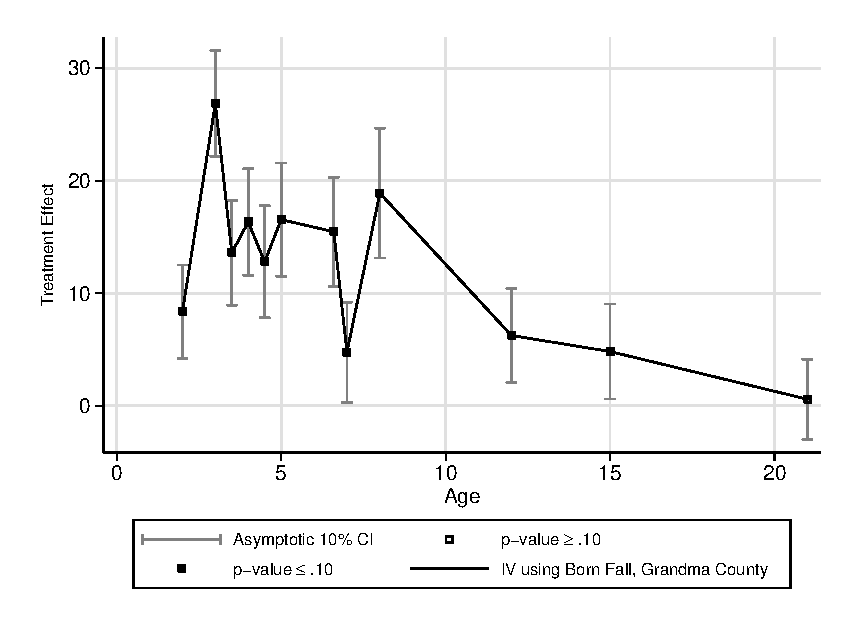
\includegraphics[width=.7\columnwidth]{output/appendixplots/main_iv_te.eps}
\floatfoot{
\footnotesize
\noindent Note: This plot presents the parameter associated with $D(\omega)$ from a regression of $Y(\omega)$ on $D(\omega)$, $Q(\omega)$, and $\mathbf{X}(\omega)$, using $R(\omega)$ and $\mathbf{Z}(\omega)(1-R(\omega))$ as instruments. The outcomes ($Y(\omega)$) are IQ tests at different ages, with a national standard deviation of 15 and a mean of 100. $\mathbf{X}(\omega)$ includes a set of controls selected from all available baseline controls to maximize explanatory power across all outcomes tested in the paper: gender of the subject, mother's IQ score, High-risk Index, and Apgar Score at 1 minute. The confidence intervals are calculated at the 10\% significance level.}
\end{figure}

\begin{figure}[H]
		\caption{Effect of Center-based Childcare on Labor Market Outcomes, Accounting for Endogenous Take-up of Alternative Preschool Using Instrumental Variables} \label{fig:mainiv2}
		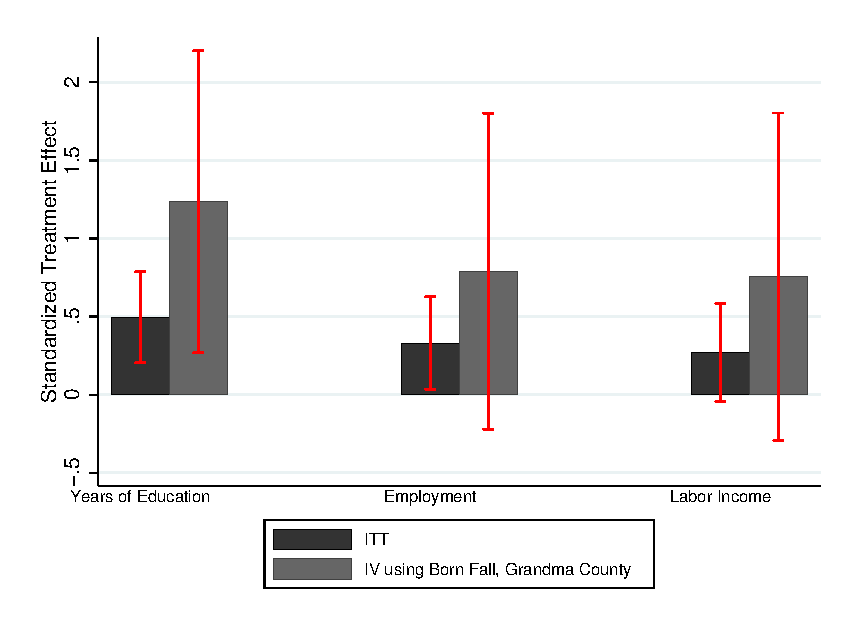
\includegraphics[width=.7\columnwidth]{output/appendixplots/main_iv_other.eps}
\floatfoot{
\footnotesize
\noindent Note: This plot presents the parameter associated with $D(\omega)$ from a regression of $Y(\omega)$ on $D(\omega)$, $Q(\omega)$, and $\mathbf{X}(\omega)$, using $R(\omega)$ and $\mathbf{Z}(\omega)(1-R(\omega))$ as instruments. The outcomes ($Y(\omega)$) are different adult outcomes labeled in the horizontal axis. $\mathbf{X}(\omega)$ includes a set of controls selected from all available baseline controls to maximize explanatory power across all outcomes tested in the paper: gender of the subject, mother's IQ score, High-risk Index, and Apgar Score at 1 minute. The confidence intervals are calculated at the 10\% significance level.}
\end{figure}

\subsubsection{Varying the Sets of Instruments}

\noindent Figure \ref{fig:ins_inter_Q_iv1} and Figure \ref{fig:ins_inter_Q_iv2} explore the sensitivity of the estimates to different sets of instruments. The pattern of results indicates that the method is generally robust to the three sets of instrumental variables that we consider. 

\begin{figure}[H]
		\caption{Effect of Center-based Childcare on IQ Scores, Accounting for Endogenous Take-up of Alternative Preschool Using Various Instrumental Variables} \label{fig:ins_inter_Q_iv1}
		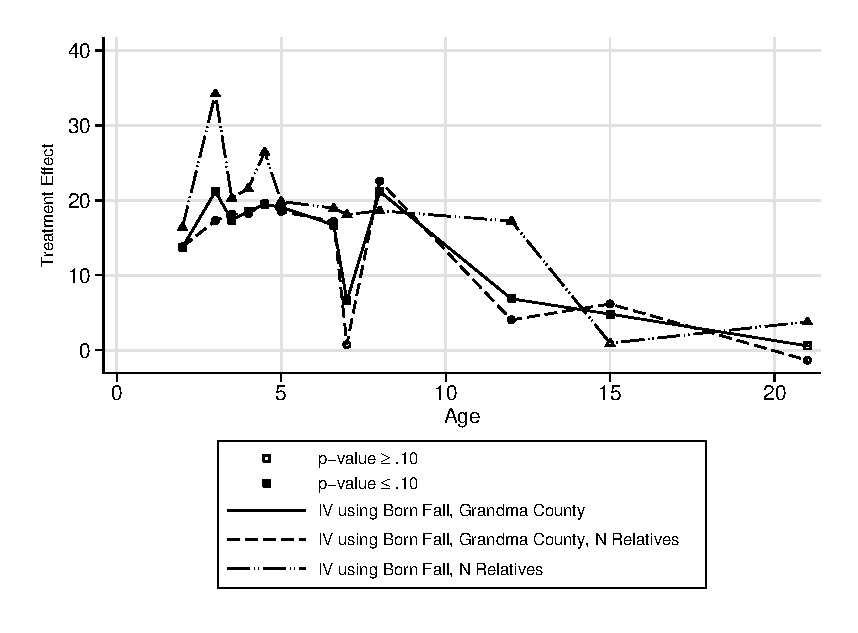
\includegraphics[width=.7\columnwidth]{output/appendixplots/ins_inter_Q_iv_te.eps}
\floatfoot{
\footnotesize
\noindent Note: This plot presents the parameter associated with $D(\omega)$ from a regression of $Y(\omega)$ on $D(\omega)$, $Q(\omega)$, and $\mathbf{X}(\omega)$, using $R(\omega)$ and $\mathbf{Z}(\omega)(1-R(\omega))$ as instruments. The outcomes ($Y(\omega)$) are IQ scores at different ages, with a national standard deviation of 15 and a mean of 100. $\mathbf{X}(\omega)$ includes a set of controls selected from all available baseline controls to maximize explanatory power across all outcomes tested in the paper: gender of the subject, mother's IQ score, High-risk Index, and Apgar Score at 1 minute. The confidence intervals are calculated at the 10\% significance level.}
\end{figure}

\begin{figure}[H]
		\caption{Effect of Center-based Childcare on Labor Market Outcomes, Accounting for Endogenous Take-up of Alternative Preschool Using Various Instrumental Variables} \label{fig:ins_inter_Q_iv2}
		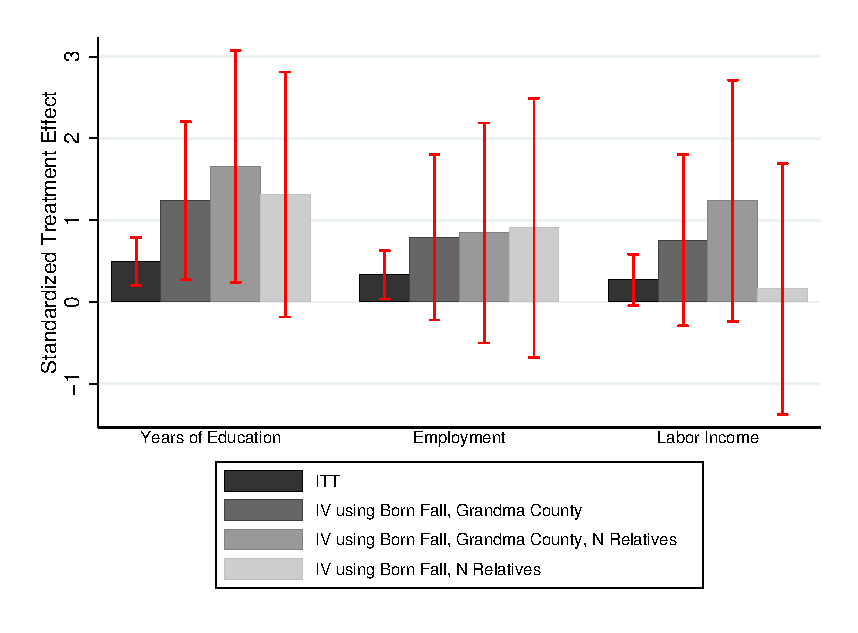
\includegraphics[width=.7\columnwidth]{output/appendixplots/ins_inter_Q_iv_other.eps}
\floatfoot{
\footnotesize
\noindent Note: This plot presents the parameter associated with $D(\omega)$ from a regression of $Y(\omega)$ on $D(\omega)$, $Q(\omega)$, and $\mathbf{X}(\omega)$, using $R(\omega)$ and $\mathbf{Z}(\omega)(1-R(\omega))$ as instruments. The outcomes ($Y(\omega)$) are different adult outcomes labeled in the horizontal axis. $\mathbf{X}(\omega)$ includes a set of controls selected from all available baseline controls to maximize explanatory power across all outcomes tested in the paper: gender of the subject, mother's IQ score, High-risk Index, and Apgar Score at 1 minute. The confidence intervals are calculated at the 10\% significance level.}
\end{figure}

\subsubsection{Varying the Specification of the Instruments}

\noindent We now present an exercise to evaluate the sensitivity of the results to different specifications of the instrumental variables. First, Figure~\ref{fig:nointer_Q_iv} and Figure~\ref{fig:nointer_Q_other} present the results using the set of instruments that are not interacted with an indicator for randomization into the control group ($1-R(\omega)$). Figure~\ref{fig:inter_Q_iv} and Figure~\ref{fig:inter_Q_other} present results not only interacting the instruments but also interacting the observed characteristics we control for. In both exercises, we use $Q(\omega)$ as the endogenous variable, along with $D(\omega)$.\\

\noindent The results follow the same patterns as before, although they change when the instruments are not interacted. This makes economic sense because the interacted instruments better represent the economic intuition we offer before: the instruments other than $R(\omega)$ are more likely to shift the decisions of the families of the control-group subjects compared to those of the treatment-group subjects.

\begin{figure}[H]
		\caption{Effect of Center-based Childcare on IQ Scores, Accounting for Endogenous Take-up of Alternative Preschool Using Various Instrumental Variables Specifications} \label{fig:nointer_Q_iv}
		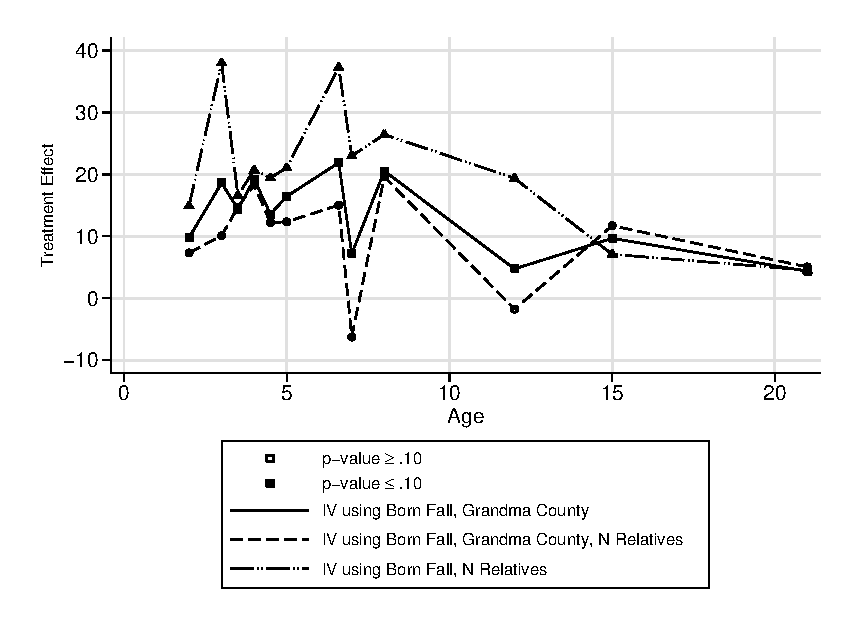
\includegraphics[width=.7\columnwidth]{output/appendixplots/nointer_Q_iv_te.eps}
\floatfoot{
\footnotesize
\noindent Note: This plot presents the parameter associated with $D(\omega)$ from a regression of $Y(\omega)$ on $D(\omega)$, $Q(\omega)$, and $\mathbf{X}(\omega)$, using $R(\omega)$ and $\mathbf{Z}(\omega)$ as instruments. $Y(\omega)$ is different IQ tests, with a national standard deviation of 15 and a mean of 100. $\mathbf{X}(\omega)$ includes a set of controls selected from all available baseline controls to maximize explanatory power across all outcomes tested in the paper: gender of the subject, mother's IQ, High-risk Index, and Apgar Score at 1 minute. The confidence intervals are calculated at the 10\% significance level.}
\end{figure}

\begin{figure}[H]
		\caption{Effect of Center-based Childcare on Labor Market Outcomes, Accounting for Endogenous Take-up of Alternative Preschool Using Various Instrumental Variables Specifications} \label{fig:nointer_Q_other}
		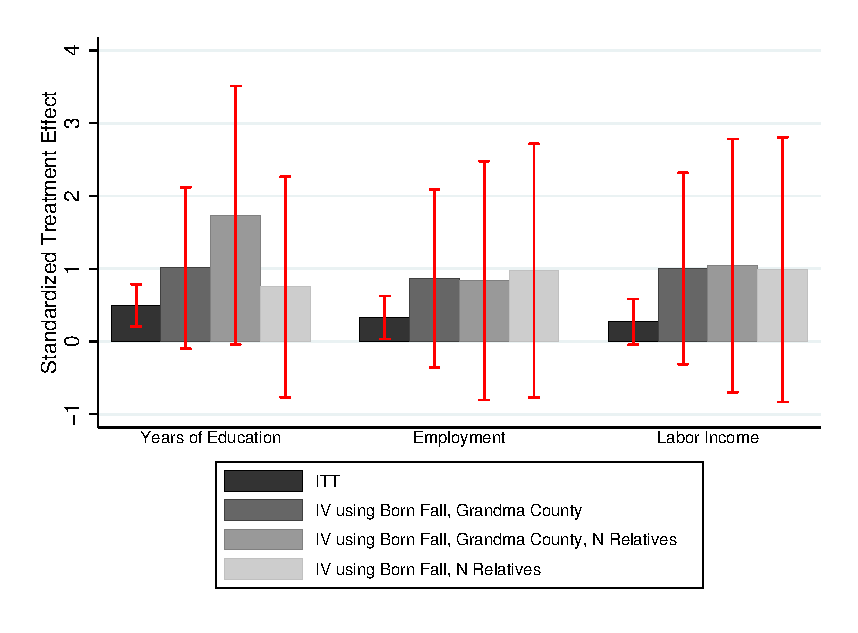
\includegraphics[width=.7\columnwidth]{output/appendixplots/nointer_Q_iv_other.eps}
\floatfoot{
\footnotesize
\noindent Note: This plot presents the parameter associated with $D(\omega)$ from a regression of $Y(\omega)$ on $D(\omega)$, $Q(\omega)$, and $\mathbf{X}(\omega)$, using $R(\omega)$ and $\mathbf{Z}(\omega)$ as instruments. The outcomes ($Y(\omega)$) are different adult outcomes labeled in the horizontal axis. $\mathbf{X}(\omega)$ includes a set of controls selected from all available baseline controls to maximize explanatory power across all outcomes tested in the paper: gender of the subject, mother's IQ score, High-risk Index, and Apgar Score at 1 minute. The confidence intervals are calculated at the 10\% significance level.}
\end{figure}

\begin{figure}[H]
		\caption{Effect of Center-based Childcare on IQ Scores, Accounting for Endogenous Take-up of Alternative Preschool Using Various Instrumental Variables Specifications} \label{fig:inter_Q_iv}
		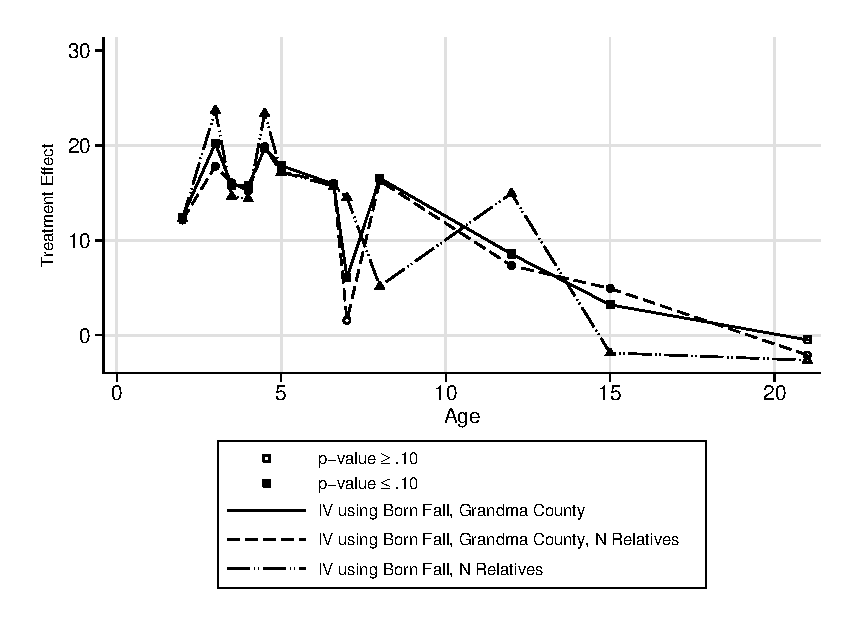
\includegraphics[width=.7\columnwidth]{output/appendixplots/inter_Q_iv_te.eps}
\floatfoot{
\footnotesize
\noindent Note: This plot presents the parameter associated with $D(\omega)$ from a regression of $Y(\omega)$ on $D(\omega)$, $Q(\omega)$ ,and $\mathbf{X}(\omega)$, using $R(\omega)$, $\mathbf{X}(\omega)(1 - R(\omega))$ and $\mathbf{Z}(\omega)(1 - R(\omega))$ as instruments. The outcomes ($Y(\omega)$) are IQ scores at different ages, with a national standard deviation of 15 and a mean of 100. $\mathbf{X}(\omega)$ includes a set of controls selected from all available baseline controls to maximize explanatory power across all outcomes tested in the paper: gender of the subject, mother's IQ score, High-risk Index, and Apgar Score at 1 minute. The confidence intervals are calculated at the 10\% significance level.}
\end{figure}

\begin{figure}[H]
		\caption{Effect of Center-based Childcare on Labor Market Outcomes, Accounting for Endogenous Take-up of Alternative Preschool Using Various Instrumental Variables Specifications} \label{fig:inter_Q_other}
		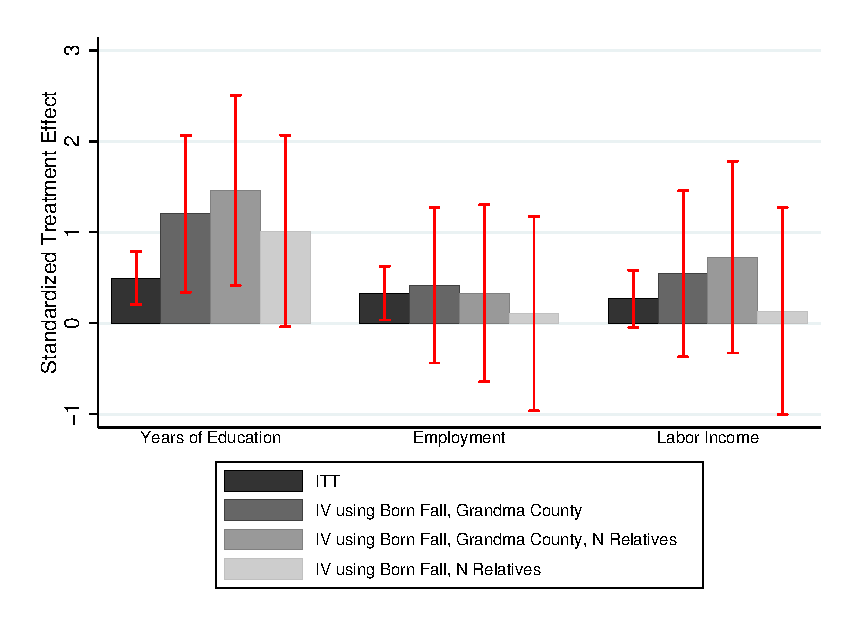
\includegraphics[width=.7\columnwidth]{output/appendixplots/inter_Q_iv_other.eps}
\floatfoot{
\footnotesize
\noindent Note: This plot presents the parameter associated with $D(\omega)$ from a regression of $Y(\omega)$ on $D(\omega)$, $Q(\omega)$, and $\mathbf{X}(\omega)$, using $R(\omega)$, $\mathbf{X}(\omega)(1 - R(\omega))$ and $\mathbf{Z}(\omega)(1 - R(\omega)$) as instruments. The outcomes ($Y(\omega)$) are different adult outcomes labeled in the horizontal axis. $\mathbf{X}(\omega)$ includes a set of controls selected from all available baseline controls to maximize explanatory power across all outcomes tested in the paper: gender of the subject, mother's IQ score, High-risk Index, and Apgar Score at 1 minute. The confidence intervals are calculated at the 10\% significance level.}
\end{figure}

\subsubsection{Varying the Parameterization of Alternative Preschool Take-up}

\noindent Now, we explore the sensitivity to the specification of $Q(\omega)$ in \eqref{eq:ivnot}. We consider two alternatives. First, we use an indicator of take-up of alternative preschool, $P(\omega)$ (Figure~\ref{fig:ins_inter_P_iv} and Figure~\ref{fig:ins_inter_P_other}). Second, we take the $\log$ of $Q(\omega)$ (Figure~\ref{fig:ins_inter_LogQ_iv} and Figure~\ref{fig:ins_inter_LogQ_other}).

\begin{figure}[H]
		\caption{Effect of Center-based Childcare on IQ Scores, Accounting for an Endogenous Indicator of Take-up of Alternative Preschool} \label{fig:ins_inter_P_iv}
		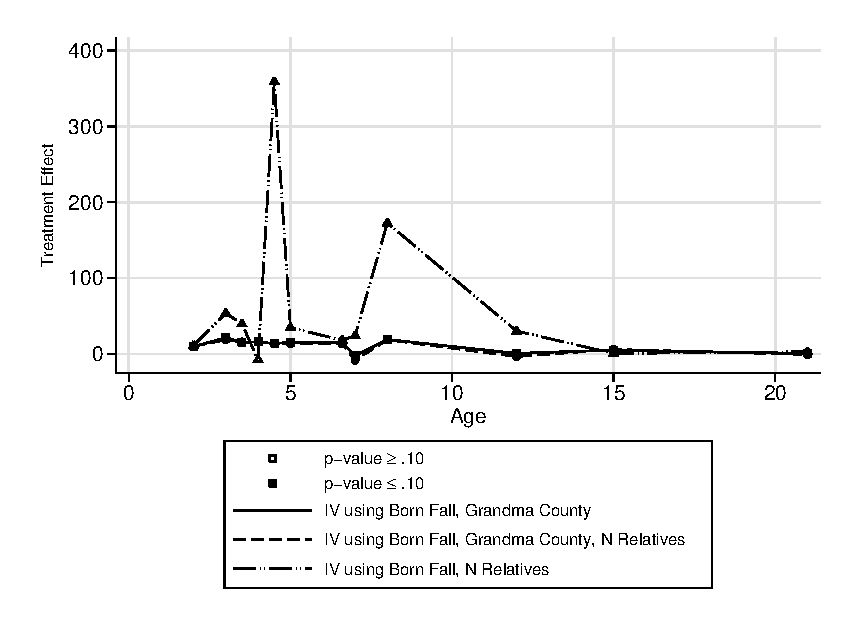
\includegraphics[width=.7\columnwidth]{output/appendixplots/ins_inter_P_iv_te.eps}
\floatfoot{
\footnotesize
\noindent Note: This plot presents the parameter associated with $D(\omega)$ from a regression of $Y(\omega)$ on $D(\omega)$, $P(\omega)$, and $\mathbf{X}(\omega)$, using $R(\omega)$, $\mathbf{Z}(\omega)(1 - R(\omega))$ as instruments. The outcomes ($Y(\omega)$) are IQ scores at different ages, with a national standard deviation of 15 and a mean of 100. $\mathbf{X}(\omega)$ includes a set of controls selected from all available baseline controls to maximize explanatory power across all outcomes tested in the paper: gender of the subject, mother's IQ score, High-risk Index, and Apgar Score at 1 minute. The confidence intervals are calculated at the 10\% significance level.}
\end{figure}

\begin{figure}[H]
		\caption{Effect of Center-based Childcare on Labor Market Outcomes, Accounting for an Endogenous Indicator of Take-up of Alternative Preschool} \label{fig:ins_inter_P_other}
		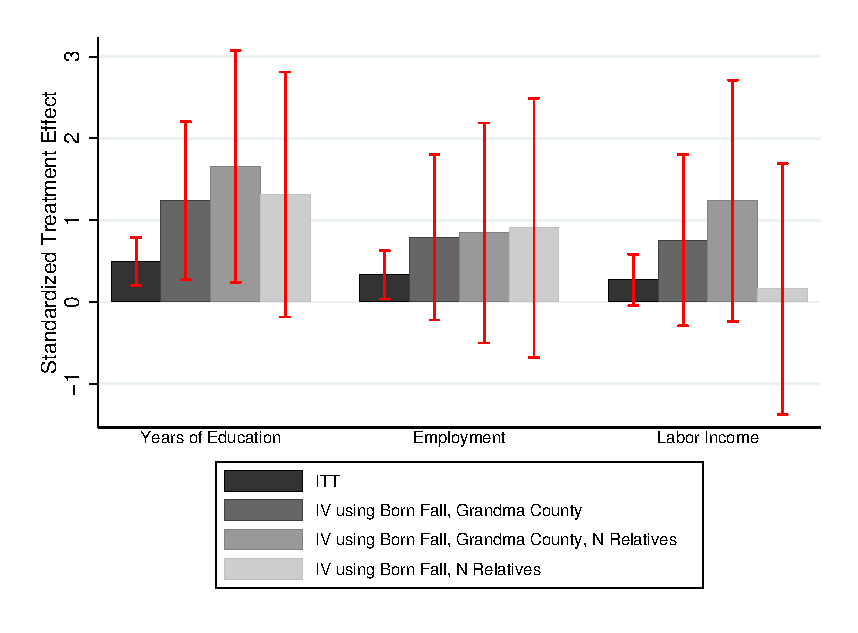
\includegraphics[width=.7\columnwidth]{output/appendixplots/ins_inter_P_iv_other.eps}
\floatfoot{
\footnotesize
\noindent Note: This plot presents the parameter associated to $D(\omega)$ from a regression of $Y(\omega)$ on $D(\omega)$, $P(\omega)$, and $\mathbf{X}(\omega)$, using $R(\omega)$, $\mathbf{Z}(\omega)(1 - R(\omega)$) as instruments. The outcomes ($Y(\omega)$) are different relevant adult outcomes labeled in the horizontal axis. $\mathbf{X}(\omega)$ includes a set of controls selected from all available baseline controls to maximize explanatory power across all outcomes tested in the paper: gender of the subject, mother's IQ score, High-risk Index, and Apgar Score at 1 minute. The confidence intervals are calculated at the 10\% significance level.}
\end{figure}

\begin{figure}[H]
		\caption{Effect of Center-based Childcare on IQ Scores, Accounting for Endogenous (log) Months of Take-up of Alternative Preschool} \label{fig:ins_inter_LogQ_iv}
		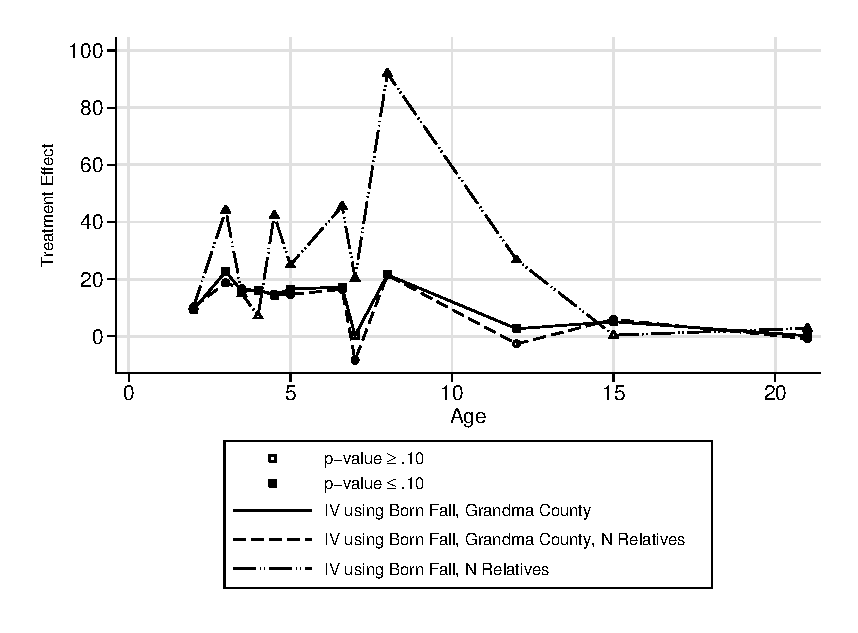
\includegraphics[width=.7\columnwidth]{output/appendixplots/ins_inter_logQ_iv_te.eps}
\floatfoot{
\footnotesize
\noindent Note: This plot presents the parameter associated with $D(\omega)$ from a regression of $Y(\omega)$ on $D(\omega)$, $\log Q(\omega)$, and $\mathbf{X}(\omega)$, using $R(\omega)$, $\mathbf{Z}(\omega)(1 - R(\omega))$ as instruments. The outcomes ($Y(\omega)$) are IQ scores at different ages, with a national standard deviation of 15 and a mean of 100. $\mathbf{X}(\omega)$ includes a set of controls selected from all available baseline controls to maximize explanatory power across all outcomes tested in the paper: gender of the subject, mother's IQ score, High-risk Index, and Apgar Score at 1 minute. The confidence intervals are calculated at the 10\% significance level.}
\end{figure}

\begin{figure}[H]
		\caption{Effect of Center-based Childcare on Labor Market Outcomes, Accounting for Endogenous (log) Months of Take-up of Alternative Preschool} \label{fig:ins_inter_LogQ_other}
		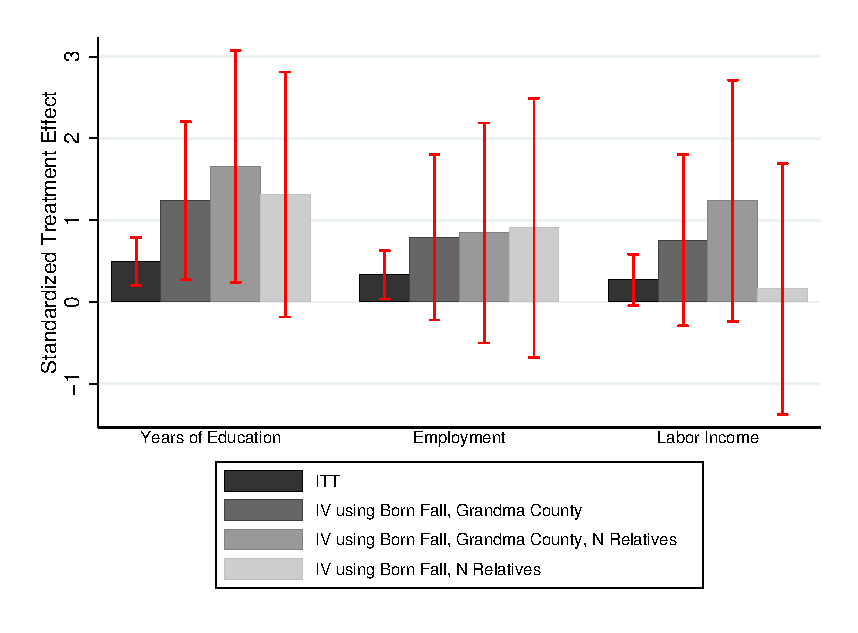
\includegraphics[width=.7\columnwidth]{output/appendixplots/ins_inter_logQ_iv_other.eps}
\floatfoot{
\footnotesize
\noindent Note: This plot presents the parameter associated with $D(\omega)$ from a regression of $Y(\omega)$ on $D(\omega)$, $\log Q(\omega)$, and $\mathbf{X}(\omega)$, using $R(\omega)$, $\mathbf{Z}(\omega)(1 - R(\omega)$) as instruments. The outcomes ($Y(\omega)$) are different adult outcomes labeled in the horizontal axis. $\mathbf{X}(\omega)$ includes a set of controls selected from all available baseline controls to maximize explanatory power across all outcomes tested in the paper: gender of the subject, mother's IQ score, High-risk Index, and Apgar Score at 1 minute. The confidence intervals are calculated at the 10\% significance level.}
\end{figure}


\subsection{Control Functions}

\noindent We now consider a control function approach. With control functions, the objective is also to simultaneously account for take-up of center-based childcare and alternative preschool. 

\subsubsection{Setup}

\noindent The method we propose is an application of the selection correction in \citet{Heckman_1979_Econometrica}. We model the selection into both endogenous variables of interest, center-based childcare and alternative preschool. The method involves three equations: (i) the outcome equation; (ii) the probability of participating in center-based childcare; (iii) a linear equation describing the number of months enrolled in preschool alternatives.\\

\noindent Let $Y^{0}(\omega)$ be the counterfactual outcome of subject $i$ when not participating in center-based childcare. Similarly, let $Y^{1}(\omega)$ be her potential outcome if she participates. We model the outcome as: 
 
\begin{eqnarray}
Y^1(\omega) &=& \alpha^1+\mathbf{X}(\omega) \mathbf{\beta}                 +\varepsilon^1(\omega) \nonumber  \\
Y^0(\omega) &=& \alpha^0+\mathbf{X}(\omega) \mathbf{\beta} + \alpha^Q Q(\omega)+\varepsilon^0(\omega).  \label{eq:potout}
\end{eqnarray}

\noindent The equation describing participation in center-based childcare is: 

\begin{equation}
D(\omega) = \left\{
        \begin{array}{ll}
        	0 &\text{if } D(\omega)^* \leq  0 \\
            1 &\text{if } D(\omega)^* > 0, \label{eq:sel1}
        \end{array}
    \right. 
\end{equation}

\noindent where we interpret $D(\omega)^*$ as a latent continuous variable representing the household's interest in sending the subject to treatment. We write

\begin{equation}
D^{*}(\omega) = \mathbf{W}(\omega) \gamma^{D} + \varepsilon^{D}(\omega), \label{eq:probitD}
\end{equation}

\noindent where $\mathbf{W}(\omega)$ is a vector that includes $\mathbf{X}(\omega)$ and $R(\omega)$ and can include variables that shift the decision to enroll subjects into ABC or CARE without shifting the counterfactual outcome of interest, $Y^{d}(\omega)$. \\

\noindent We model the selection into months of alternative preschool as a linear equation with fixed coefficients, assuming homogeneous treatment effects:

\begin{equation}
Q(\omega) = \mathbf{W}(\omega) \gamma^{Q} + \varepsilon^{Q}(\omega), \label{eq:selq}
\end{equation}

\noindent In general, the unobserved variables in each of these equations are correlated. We assume that they are distributed as follows: 

\begin{equation}
        \left[ \begin{array}{l}
        	 \varepsilon(\omega)^1 \\
            \varepsilon(\omega)^0 \\
            \varepsilon(\omega)^D
        \end{array} \right]  \sim \mathcal{N} \left[ \left( \begin{array}{l}
        	 0 \\
           0 \\ 
           0
        \end{array} \ \right), 
                \left( \begin{array}{llll}
        	 \sigma_{1}^2 & \sigma_{1,0} & \sigma_{1,D}   \\
             \sigma_{1,0} & \sigma_{0}^2 & \sigma_{0,D}   \\
             \sigma_{1,D} & \sigma_{0,D} & 1 
        \end{array} \right) \right],  \label{eq:udist}
\end{equation}

\noindent where we normalize $\var \left( \varepsilon^D(\omega) \right) =1$.\\

\noindent Further, we assume that 
\begin{equation}
\mathbb{E}\left[\varepsilon(\omega)^0|D(\omega)=0,\mathbf{W}(\omega),\varepsilon^{Q}(\omega),Q(\omega)=q\right]=\sigma^{0,Q}\varepsilon^{Q}(\omega)+\mathbb{E}\left[\varepsilon(\omega)^0|D(\omega)=0,\mathbf{W}(\omega)\right].
\label{eq:E[epsilon0]}
\end{equation}

\subsubsection{Identification}

\noindent The following steps identify the parameters of interest. First, we estimate the parameters characterizing the decision to enroll the subject in center-based childcare. We exploit the assumption that $\varepsilon(\omega)^D \sim \mathcal{N} \left( 0, 1 \right)$ in \eqref{eq:udist} and estimate the parameters in \eqref{eq:probitD} using a probit model.\\

\noindent Second, we approximate the unobserved term relevant to the choice of $Q(\omega)$. We take the coefficients in \eqref{eq:selq} to obtain an estimate for $\varepsilon^{Q}(\omega)$. By linearly conditioning on this term, we account for the correlation between the error term in the decision for $Q(\omega)$ and the error term in the outcome equation, $\varepsilon(\omega)^0$.\\

\noindent Third, we estimate the coefficients in the outcome equation using the proxies for the unobserved components. We rewrite \eqref{eq:potout} using conditional expectations:

\begin{eqnarray}
\mathbb{E}\left[Y(\omega)^1|D(\omega)=1,\mathbf{W}(\omega)\right]                         &=& \alpha^1+\mathbf{X}(\omega)\mathbf{\beta}              +\mathbb{E}\left[\varepsilon(\omega)^1|D(\omega)=1,\mathbf{W}(\omega)      \right] \nonumber \\
\mathbb{E}\left[Y(\omega)^0|D(\omega)=0,\mathbf{W}(\omega),\varepsilon^{Q}(\omega),Q(\omega)=q\right] &=& \alpha^0+\mathbf{X}(\omega)\mathbf{\beta} +\alpha^Q q \label{eq:condout} \\ \nonumber && \quad + \mathbb{E}\left[\varepsilon(\omega)^0|D(\omega)=0,\mathbf{W}(\omega),\varepsilon^{Q}(\omega),Q(\omega)=q\right].
\end{eqnarray}

\noindent Once we condition on the proxy for $\varepsilon^{Q}(\omega)$, the error term in the outcome equations only depends on the selection into center-based childcare. The conditional error terms in \eqref{eq:condout} can be specified using control functions.\\ 

\noindent For subjects enrolled in treatment, the control function is: 
\begin{equation}
\mathbb{E} \left[\varepsilon(\omega)^1|D(\omega)=1,\mathbf{W}(\omega) \right]=\sigma_1\frac{\phi \left( \mathbf{W}(\omega) \gamma^D \right) }{ \Phi \left( \mathbf{W}(\omega) \gamma^D \right) }. \label{eq:contam}
\end{equation}

\noindent For subjects not enrolled in the treatment, the control function is:
\begin{equation}
\mathbb{E} \left[\varepsilon(\omega)^0|D(\omega)=0,\mathbf{W}(\omega),\varepsilon^{Q}(\omega),Q(\omega)=q\right]= \sigma^{0,Q}\varepsilon^{Q}(\omega) - \sigma_0 \frac{\phi\left(\mathbf{W}(\omega)\gamma^D\right)}{\Phi\left( - \mathbf{W}(\omega) \gamma^D \right) }. \label{eq:home}
\end{equation}

\subsection{Estimates}

\noindent By including the control functions, we can recover consistent estimates of the parameters in \eqref{eq:potout} through a linear regression. The effect of center-based childcare is the difference of the intercepts in the two outcome equations.\\

\noindent The charts below present the estimates for the parameter associated with $D(\omega)$. That is, the effect of participating in center-based childcare relative to a counterfactual of receiving no preschool alternative. As before, we present results for IQ scores at different ages and for a set of relevant adult outcomes. The results are not compelling, as they present irregularities over the life cycle that differ from the rest of results we present in the main paper and throughout this appendix. 

\begin{figure}[H]
		\caption{Effect of Center-based Childcare on IQ Scores, Accounting for Endogenous (log) Months of Take-up of Alternative Preschool} \label{output/appendixplots/Q_cf_te.eps}
		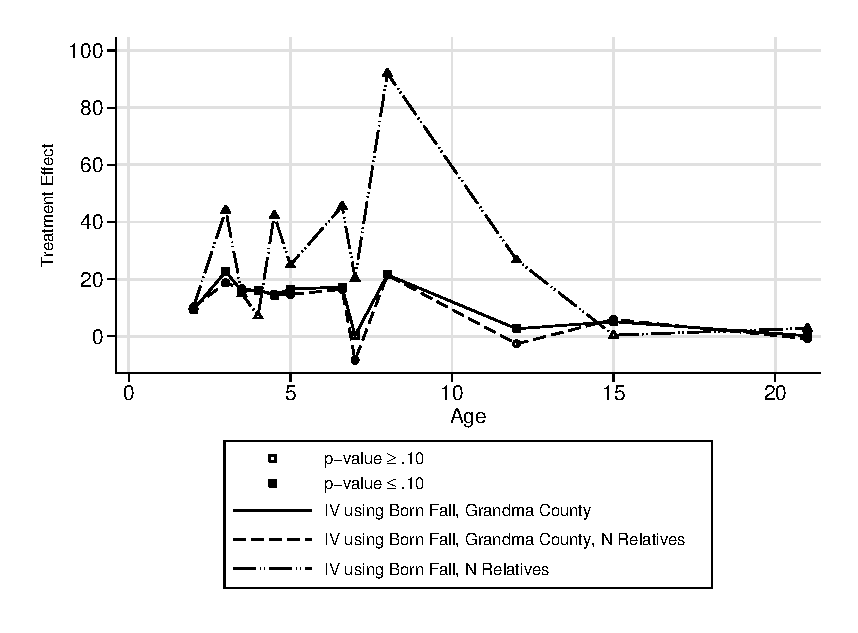
\includegraphics[width=.7\columnwidth]{output/appendixplots/ins_inter_logQ_iv_te.eps}
\floatfoot{
\footnotesize
\noindent Note: This plot presents the parameter associated with $D(\omega)$ estimated using Control Functions as described in the text. The outcomes ($Y(\omega)$) are IQ scores at different ages with a national standard deviation of 15 and a mean of 100.  $D(\omega)=1$ for subjects that participate in ABC or CARE center-based childcare, and $D(\omega)=0$ for subjects who do not participate in treatment. $Q(\omega)$ is the number of months attending preschool. It is coded as zero for subjects participating in ABC or CARE. $\mathbf{X}(\omega)$ includes a set of controls selected from all available baseline controls to maximize explanatory power across all outcomes tested in the paper: gender of the subject, mother's IQ score, High-risk Index, and Apgar Score at 1 minute.}
\end{figure}

\begin{figure}[H]
		\caption{Effect of Center-based Childcare on Labor Market Outcomes, Accounting for Endogenous (log) Months of Take-up of Alternative Preschool} \label{output/appendixplots/Q_cf_te.eps}
		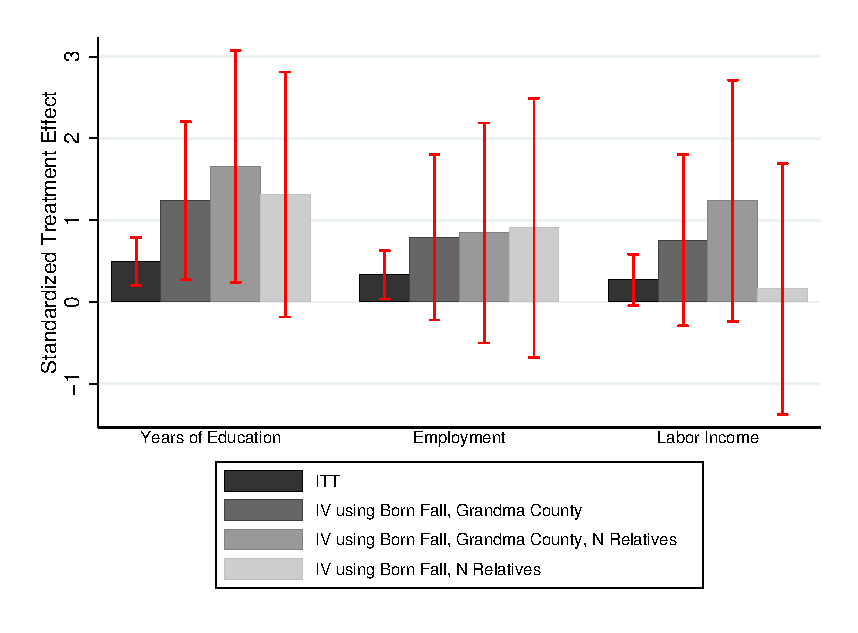
\includegraphics[width=.7\columnwidth]{output/appendixplots/ins_inter_logQ_iv_other.eps}
\floatfoot{
\footnotesize
\noindent Note: This plot presents the parameter associated with $D(\omega)$ estimated using Control Functions as described in the text. The outcomes ($Y(\omega)$) are different adult outcomes labeled in the horizontal axis.  $D(\omega)=1$ for subjects that participate in ABC or CARE center-based childcare, and $D(\omega)=0$ for subjects who do not participate in treatment. $Q(\omega)$ is the number of months attending preschool. It is coded as zero for subjects participating in ABC or CARE. $\mathbf{X}(\omega)$ includes a set of controls selected from all available baseline controls to maximize explanatory power across all outcomes tested in the paper: gender of the subject, mother's IQ score, High-risk Index, and Apgar Score at 1 minute.}
\end{figure}

\setcounter{figure}{0}  \renewcommand{\thefigure}{E.\arabic{figure}}
\setcounter{table}{0}   \renewcommand{\thetable}{E.\arabic{table}}
\section{Assessing Common Critiques to ABC} \label{appendix:assessingcc}

\noindent This section of the appendix assesses some of the critiques to ABC, which could apply to CARE as well. The critiques focus on the first phase of the program, to which we refer simply as ABC in this section of the appendix. We consider the following categories of critiques: (i) validity of treatment effects given early differences between treatment and control groups, (ii) fadeout of the treatment effect on cognitive outcomes, and (iii) compromised randomization. \\

\subsection{Treatment Effects vs. Early Differences Between Groups}

\noindent The first critique we assess is that of \citet{Spitz_1992_ABC-Retardation}. The author asks if ABC prevented socio-cultural mental retardation. He focuses on different measures of cognition, and generically calls them IQ. His main focus is on the raw mean difference between the treatment and the control groups in the Bayley Mental Development Index (MDI) from the Bayley Scales of Infant Development and Infant Behavior (BSID) at 1 year of age.\footnote{The Bayley Mental Development Index (MDI) is a standard measure of cognition at taken between ages 0 and 2 \citep{Childrens-Health_2016_Bayley-Scales}.} He finds a noticeable disparity in the mean difference between cohorts 1 and 2 and cohorts 3 and 4, as early as six months after the treatment began. As \citet{Spitz_1992_ABC-Retardation} argues, this difference, displayed in Table~\ref{table:cohorts}, is conspicuous. Importantly, the author fails to note that the mean differences have noticeably high standard errors.

\begin{table}[H] 
\begin{threeparttable}
\caption{Treatment - Control Mean Difference by Cohort, ABC}
\label{table:cohorts}
\centering 
\begin{tabular}{lcc} \toprule
 & (1) & (2) \\
 & Bayley MDI, 12 Months & Bayley MDI, 24 Months \\ \midrule
 &  &  \\\
Cohort 1 & 4.841 & -2.901 \\
 & (6.013) & (5.926) \\
Cohort 2 & 0.071 & 1.882 \\
 & (6.013) & (5.830) \\
Cohort 3 & 9.143 & 10.038 \\
 & (5.801) & (5.926) \\
Cohort 4 & 7.829 & 13.713 \\
 & (5.801) & (5.830) \\ \\ \midrule
Observations & 112 & 110 \\
$R^2$ & 0.055 & 0.110 \\ \bottomrule
 \end{tabular}
\begin{tablenotes}
\footnotesize
\item Note: This table displays the mean difference between the treatment and control groups in two measures of the Bayley Mental Development Index, for ABC. Homoskedastic, asymptotic standard errors are in parentheses.
\end{tablenotes}
\end{threeparttable}
\end{table}

\noindent \citet{Spitz_1992_ABC-Retardation} states that ``an essential question is whether the differences at 6 months of age were due to the intervention or were preexisting'' \citep[][p. 230]{Spitz_1992_ABC-Retardation}. \citet{Spitz_1992_ABC-Retardation} proceeds with speculative exercises that lead him to state that it is questionable to conclude that the mean difference between the treatment and control groups as early as 6 months of age is a consequence of the treatment.\footnote{The exact quote is: ``Even if the differences between experimental and control groups at 6 months of age were a consequence of the first few months of intervention, which is questionable, the negligible additional effects after age 4.5 more years in the program should at least make one cautious about this kind of intervention's potential [\ldots]'' \citep[][p. 235]{Spitz_1992_ABC-Retardation}. We assess the former point before getting to the latter.}\\

\noindent His argument stems from not receiving information on the maternal characteristics, which he considers fundamental for his analysis to comparing test scores over the years.\footnote{He does not note that tests scores \textit{do not have a well-defined scale} and are hard to compare.}\\ 

\noindent We present some annotations with respect to the comments in \citet{Spitz_1992_ABC-Retardation}.\\ 

\noindent \textbf{1. Mothers do not significantly differ in observed characteristics between the treatment and the control groups in any ABC cohort.} When jointly testing the hypothesis of differences in a battery of observed characteristics, we fail to reject any difference between the families of the subjects (see Table~\ref{tab:baseline_coh1} to Table~\ref{tab:baseline_coh4}). Even when the point estimates present some differences, they are minimal. For example, treatment-group mothers differ from control-group mothers, on average, by having one point higher IQ score (the population standard deviation is 15 points).\\

\noindent \textbf{2. Other early childhood education programs have generated gains in cognition very early in life, as soon as a year after the start of the program.} A more recent program, the Infant Health and Development Program (IHDP), treated children from ages 0 to 3. \citet{Gross_Spiker_etal_1997_BOOKHelpinglowbirth} thoroughly describe this program. A lot of its elements were based on ABC and CARE. The program offered, on average, eight hours a week of center-based childcare from ages 1 to 3, weekly home visits from ages 0 to 1, and bi-monthly home visits from ages 1 to 3. Measures of the Bayley MDI at 12 and 24 months are available. The most intensive part of the treatment, center-based childcare, began in IHDP at 12 months of age while it began in ABC at birth. As in ABC, after a few months of center-based childcare, the effects on cognition were substantial in IHDP.

\begin{table}[H] 
\begin{threeparttable}
\caption{Treatment - Control Mean Difference, IHDP}
\label{table:ihdp}
\centering 
\begin{tabular}{lcc} \hline \hline
 & (1) & (2) \\
 & Bayley MDI, 12 Months & Bayley MDI, 24 Months \\ \hline
 &  &  \\\
Mean Treatment - Mean Control & 0.142 & 9.958 \\
 & (0.968) & (1.498) \\
 &  &  \\ \hline
Observations & 893 & 910 \\
$R^2$ & 0.000 & 0.067 \\ \hline \hline  
\end{tabular}
\begin{tablenotes}
\footnotesize
\item Note: This table displays the mean difference between the treatment and control groups in two measures of the Bayley Mental Development Index, for the Infant Health and Development Program using the principal analysis sample. Robust standard errors clustered by state and an indicator of weight below 2,000 grams in parentheses.
\end{tablenotes}
\end{threeparttable}
\end{table}


\noindent \textbf{3. The effects on cognition are sustained throughout childhood and up to age 21 even when partialing out the Bayley MDI at ages 12 and 24 months.} When partialing out from a linear regression the score in the Bayley MDI tests both at 12 and 24 months of age, the treatment effects on cognition, measured by the mean difference in IQ scores at different ages between the treatment and control groups, are still significant and are sustained up to age 21 (see Figure~\ref{fig:treatiqsabc}).

\begin{figure}[H]
		\caption{Treatment Effects on IQ, ABC} \label{fig:treatiqsabc}
		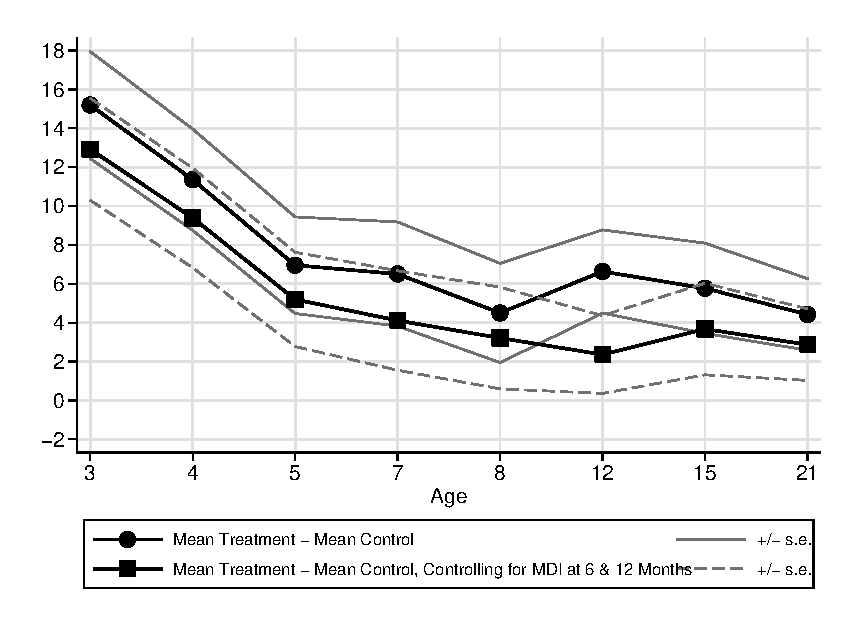
\includegraphics[width=.9\columnwidth]{output/abc_mdifixing_2.eps}
\floatfoot{
\footnotesize
\noindent Note: This figure displays the mean difference in IQ scores at different ages between the treatment and control groups, pooling males and females. The line with circles represents the raw difference. The line with squares represents the difference when linearly controlling for the Bayley Mental Development Index at 12 and 24 months.}
\end{figure}

\noindent The author raises an additional concern. He states that even if the early-life effects on the Bayley MDI were valid, the effects were not long-lasting. When doing so, he exclusively refers to the effects the program had on cognition. As we document throughout the main paper, however, ABC had effects on a wide set of life-cycle outcomes, which perhaps are more important than the effects on cognition if measured by the economic gains they generate. Examples include: employment at age 30 for males, high-school graduation for females, and a variety of health measures at age 34 for males. We document these effects in the main paper.\\

\subsection{Fadeout of Treatment Effects}

\noindent This sustained effect on life-cycle outcomes relates to another category of criticism of ABC---the fadeout of treatment effects after the actual treatment period.\footnote{See, for example, \citet{Besharov-etal_2011_ABCProject}.} Based on the fadeout of the effects on cognition and age-21 outcomes, some studies claim that ABC had no sustained long-term effects. In addition to the evidence we cite above, it is important to add the following.\\

\noindent  \textbf{4. The treatment effects of ABC differed by gender.} For example, we find substantial effects on employment for males and high-school graduation for females. This does not mean that the program did not work. It means that market conditions could have affected the way in which the treated subjects benefited from the program's effects.\\

\subsection{Compromised Randomization}

\noindent The third and last critique we assess is that of compromised randomization.\footnote{See for example \citet{Baumeister-Bacharach_2000_Early-Generic} and the multiple studies cited there.} The main critique to the program in this respect is that seven children in the treatment group did not comply to their initial assignment and one subject switched from control to treatment status (see Table~\ref{table:abccompromises}, which we reproduce from the main paper). Although we document more cases of compromised randomization, we start by assessing these eight cases.\footnote{Our main methodology assesses all the cases except the four subjects for whom we do not have data at all. We are not able to account for them because our method is based on observing at least some baseline characteristics. See Section~\ref{section:methodology} in the main paper for more details.}\\

\noindent First, we propose a method to assess the non-compliance of six subjects for whom we have data available from ages 0 to 8. This allows for the possibility of adjusting the mean difference between the treatment and the control groups, using a standard Bloom estimator \citep{Bloom_1984_ER}. This estimator accounts for compliance, by weighting the mean difference by a measure of the probability of compliance. It takes the following form: 

\begin{equation}
\Delta^{\textbf{Bloom}} = \frac{\mathbb{E} \left[ Y | R = 1 \right] - \mathbb{E} \left[ Y | R = 0 \right] }{\mathbb{E} \left[ D | R = 1 \right] - \mathbb{E} \left[ D | R = 0 \right]}, 
\end{equation}

\noindent where $R$ indicates randomization into treatment, $D$ indicates treatment take-up, and $Y$ is an outcome of interest.\\

\noindent This estimator coincides with the instrumental variable estimator of the parameter in a linear regression of an outcome on a single explanatory variable, e.g. treatment take-up. As \citet{Angrist_Imbens_ea_1996_JASA} show, under certain assumptions it can be interpreted as the average treatment effect for those individuals induced to take up treatment by the instrument. This interpretation has various weaknesses \citep{Heckman_Urzua_etal_2006_REStat,Heckman_Urzua_2010_JoE}.\\

\noindent To compare the mean difference and the Bloom estimator we consider two measures of cognition, which are commonly used when evaluating ABC and are available for these six subjects: the Stanford-Binet Intelligence Scale at age 3 and the Wechsler Preschool and Primary Scale of Intelligence at age 5. Table~\ref{table:nc1} presents the results and shows that the differences are minimal. \textbf{5. Adjusting for the non-compliance of these six subjects makes little difference} when assessing outcomes that we observe for these subjects. 

\begin{table}[H] 
\begin{threeparttable}
\caption{Assessing Non-compliance in ABC, Exercise 1}
\label{table:nc1}
\centering 
\begin{tabular}{ccccc} \toprule
 & (1) & (2) & (3) & (4) \\
 & IQ, Age 3 & IQ, Age 3  & IQ, Age 5 & IQ, Age 5 \\ \midrule
 &  &  & & \\\
Treatment - Control Mean Difference & 14.970 &  & 6.398 &  \\
 & (2.794) &  & (2.494) &  \\
Bloom &  & 16.245 &  & 6.943 \\
 &  & (2.877) &  & (2.643) \\ \midrule
Observations & 100 & 100 & 100 & 100  \\
 $R^2$ & 0.227 & 0.289 & 0.063 & 0.088 \\ \bottomrule
 \end{tabular}
\begin{tablenotes}
\footnotesize
\item Note: This table displays the mean difference between the treatment and control groups and the same difference adjusted for non-compliance (Bloom estimator) in two measures of IQ, the Stanford-Binet IQ Score at age 3 and the Wechsler Preschool and Primary Scale of Intelligence at age 5. Homoskedastic, asymptotic standard errors are in parentheses.
\end{tablenotes}
\end{threeparttable}
\end{table}


\noindent Second, we propose a method to account for non-compliance of the four subjects for whom we have no data at all. We reproduce the estimates in Table~\ref{table:nc2}, assigning the lowest score across all the subjects in the treatment group to each of these four children. For each of the tests we consider, the lowest score was 71 for both the age-3 and the age-5 measures. \textbf{6. Even when assigning the lowest score to the subjects who did not comply to treatment and for whom no data are available, the mean difference between treatment and control is sizable and not significantly different from the baseline cases where we do not adjust for non-compliance cases} (columns (1) and (3) in Table~\ref{table:nc1}).

\documentclass[]{article}
\setlength{\pdfpagewidth}{8.5in} \setlength{\pdfpageheight}{11in}
\begin{document}
\begin{tabular}{lcccc} \hline
 & (1) & (2) & (3) & (4) \\
 & iq3y\_itt & iq3y\_iv & iq5y\_itt & iq5y\_iv \\
VARIABLES & IQ at age 3y months & IQ at age 3y months & IQ at age 5y months & IQ at age 5y months \\ \hline
 &  &  &  &  \\
Randomization into center-based care (ABC and CARE) & 12.908*** &  & 4.284 &  \\
 & (2.901) &  & (2.647) &  \\
Indicator for the actual treatment receipt for center-based care &  & 15.111*** &  & 5.016* \\
 &  & (3.061) &  & (2.960) \\
 &  &  &  &  \\
Observations & 104 & 104 & 104 & 104 \\
 R-squared & 0.163 & 0.306 & 0.025 & 0.093 \\ \hline
\end{tabular}
\end{document}


\noindent Finally, we note that our methodology in Section~\ref{section:methodology} and the results we present in Section~\ref{section:results} account for the remainder of randomization compromises, as when the families moved or abandoned the study later on. \textbf{7. The results are not greatly sensitive to adjusting for the rest of the randomization compromises}, as we show in Section~\ref{section:results}.

\setcounter{figure}{0}  \renewcommand{\thefigure}{F.\arabic{figure}}
\setcounter{table}{0}   \renewcommand{\thetable}{F.\arabic{table}}
\section{Calculating the Benfit-to-cost Ratio and the IRR}

\noindent We estimate the benefit-to-cost ratio and the  internal rate of return of participation in ABC and CARE for the \textit{average participant} of the program. Let $B_{r,t}$ denote benefits and  $C_{r,t}$ denote costs for group $r$ at age $t$. Then $r$ takes either two values, $0$ for children randomized into the control group or $1$ for children randomized into the treatment group.\\ 

\noindent Both $B_{r,t}$ and $C_{r,t}$ are in 2014 USD and discounted to $t = 0$. Thus, the benefits $B_t = B_{1,t} - B_{0,t}$ and costs $C_t = C_{1,t} - C_{0,t}$ associated with program participation are the differences between the counter-factual benefits and costs. We use the counter-factual notation for costs because the costs for the control group are not zero: the control group children received some services from the ABC and CARE centers and some attended alternative care programs. \\

\noindent The estimate for the benefit-to-cost ratio is
\begin{align}
\mathbf{E} \left( \frac{ \sum_{t=0}^T B_t}{\sum_{t=0}^T C_t} \right).
\end{align}

\noindent The estimate for the internal rate of return is the value $\rho$ that solves:

\begin{align}
\sum_{t=0}^T \frac{ \mathbf{E} (B_t - C_t)}{(1+\rho)^t} = 0.
\end{align}

\setcounter{figure}{0}  \renewcommand{\thefigure}{G.\arabic{figure}}
\setcounter{table}{0}   \renewcommand{\thetable}{G.\arabic{table}}

\section{Accounting for Attrition} \label{appendix:attrition}

\noindent We use a standard inverse probability weighting (IPW) scheme based on a logit model that predicts attrition using baseline characteristics.\footnote{\citet{Horvitz_Thompson_1952_JASA}.} We detail the identification of this scheme below. We describe our model selection process and the selected logit models in Tables \ref{table:nonipw}--\ref{table:ms_attrit_pooled} in Appendix \ref{app:method_identify}. We use the Akaike Information Criteria (AIC) to select the model with the best predictive ability. We use the same notation as in Section~\ref{section:cbamethodology} and a vector of background characteristics used in the randomization protocol; $W$ are background characteristics not used in this protocol.\\

\noindent Formally, let $A=1$ denote the case where we observe $Y$ and $A=0$ denote otherwise. We assume $A$ is independent of $Y$ conditional on $Z$, $R$, $X$, and $W$. Thus,

\begin{assumption} \label{ass:attr}
	\begin{align*}
		A \independent Y | W, Z, X, R.
	\end{align*}
\end{assumption}

\noindent Based on this assumption, we identify $\mathbb{E}[Y_r]$ as follows:

\begin{align} \label{eq:case2}
\mathbb{E}[Y_r] & = \int y f_{Y_r|Z}(y) f_Z(z) dydz \\ \nonumber
	           & = \int y f_{Y|Z,R=r}(y) f_Z(z) dydz \\ \nonumber
				& = \int y f_{Y|R=r,W,Z,X}(y) f_{W,X|R=r}(w,x) f_Z(z) dydxdwdz \\ \nonumber
				& = \int y f_{Y|R=r,W,Z,X,A=1}(y) f_{W,X|R=r,Z}(w,x) f_Z(z) dydxdwdz
\end{align}
\noindent where each component of \eqref{eq:case2} is straightforward to recover from the data. Using Bayes' Theorem, we can write an equivalent expression to make the IPW scheme explicit. That is, we apply Bayes' Theorem to $f_{W,X|R=r,Z}(w,x)$ and $f_Z(z)$ to obtain

\begin{equation*}
f_{W,X|R=r,Z}(w,x) = \frac{f_{W,X|R=r,Z,A=1}(w,x) P(A=1|R=r,Z)}{P(A=1|R=r,W,Z,X)}
\end{equation*}
and
\begin{equation*}
	f_Z(z) = \frac{f_{Z|R=r,A=1}(z) P(R=r,A=1)}{P(R=r,A=1|Z)}.
\end{equation*}
\noindent Then, we substitute these expressions into \eqref{eq:case2} to get

\begin{align*} \label{eq:case2ipw}
\mathbb{E}[Y_r] & = \int y f_{Y,X,W,Z|R=r,A=1}(y,x,w,z) \frac{P(R=r,A=1) P(A=1|R=r,Z)}{P(R=r,A=1|Z) P(A=1|R=r,W,Z,X)} dydxdwdz \\
	            & = \int y f_{Y,X,W,Z|R=r,A=1}(y,x,w,z) \frac{P(R=r,A=1)}{P(R=r|Z) P(A=1|R=r,W,Z,X)} dydxdwdz. \\
\end{align*}

\noindent Assumption \ref{ass:attr} generalizes the matching assumption of \citet{Campbell_Conti_etal_2014_EarlyChildhoodInvestments}. It conditions not only on pre-program variables but on fully observed post-treatment variables, $X$. This enables us to account  for two types of selection:  (i) selection into treatment; and (ii) selection into item response. The corresponding sample estimator for $\mathbb{E}[Y_r]$ is

\begin{align*}
\sum_{i \in \mathcal{I}} y(\omega) a_{i} w_{i,r} \mathbf{1}(r_i = r)
\end{align*}
\noindent where $\mathcal{I}$ indexes the individuals in the sample, $a_i$ indicates whether we observe $Y$ for individual $i$, and

\begin{align*}
	w_{i,r} = \frac{1}{\pi_r(z_i) \alpha(r_i,w_i,z_i,x_i)} \frac{1}{\sum_k{\frac{\mathbf{1}(r_i = r) \mathbf{1}(a_i = 1)}{\pi_r(z_k)\alpha(r_k,w_k,z_k,x_k)}}},
\end{align*}
\noindent with $\pi_r(z) := P(R=r|Z=z)$ and $\alpha(r,w,z,x) := P(A=1|R=r,W=w,Z=z,X=x)$. The weight $\pi_r$ corrects for selection into treatment based on pre-program variables $Z$. The weight $\alpha$ corrects for item non-response based on $R, W, Z, X$. \\


\setcounter{figure}{0}  \renewcommand{\thefigure}{H.\arabic{figure}}
\setcounter{table}{0}   \renewcommand{\thetable}{H.\arabic{table}}
\section{Details on Interpolation and Extrapolation} \label{appendix:methodology}

\subsection{Identifying Treatment Effects}
\label{app:method_identify}

\noindent In the main paper, we discuss three cases of attrition. Below, we elaborate on the methodology we use for each case. \\

\subsubsection{Complete Data}
\label{app:method_fullobs}

\noindent  In the case where we have complete data, we only need to address the compromised randomization
of treatment status in our empirical estimates (see Section \ref{section:methodology}). \\

\noindent Randomization into treatment and control for each cohort occurred after the cohort was split
into two subsamples balanced by gender, maternal IQ,
and number of siblings. Subjects from each subsample were then matched on HRI, and randomized
into their respective experimental groups. Sex, maternal IQ, number of siblings, and HRI
therefore comprise $Z$. To obtain an
unbiased estimate of the treatment effect, we regress the outcome variable on treatment status,
controlling for those four baseline variables, as well as for cohort. \\

\noindent We estimate on 1,000 bootstrap resamples of the original ABC/CARE data to estimate sampling uncertainty. We take the mean of the empirical bootstrap distribution as our point estimate, and the standard deviation
of the distribution as the standard error. We estimate these effects on the
whole ABC/CARE sample, as well as the male and female subsamples. This allows us to generate
rates of return and benefit/cost ratios for the male subsample, the female subsample, and the pooled sample. \\
%Moreover, we are able to obtain more precise estimates of the treatment
%effect for males, as the data for females generally exhibit more noise. See Table \ref{table:nonipw} for the list of outcomes to which we apply this method.


\subsubsection{Partially Observed Outcomes}
\label{app:method_partialobs}

\noindent Given the small sample sizes of the ABC/CARE data, we consider outcome variables with fewer than 100 observations
as having a sizable rate of attrition. These variables include parental income at ages 2, 3, 4, 5, 9, 12,
and 15, for which we observe no more than 91 subjects at any given age; and the health survey at
age 34, for which we observe no more than 72 subjects. \\

\noindent We weight each subject by
his/her propensity to select into treatment and propensity to respond. We estimate the
former with a logit model for treatment status, controlling for baseline
variables used to determine randomization into treatment status: cohort,
maternal IQ, number of siblings, HRI, and sex (in the case of pooled estimates). \\

\noindent To estimate the propensity to respond, we estimate a logit model of observing the outcome,
controlling for treatment status and three additional covariates. The additional covariates are
chosen amongst a set of variables likely to be correlated with non-response rates for the outcome variable.
This set of variables includes baseline characteristics determining randomization,
baseline variables other than randomization, and observed adult outcomes potentially affected by
treatment. To select these variables, we estimate the
aforementioned logit model controlling for treatment status and every three-variable combination from
the described set of variables. The model with the lowest Akaike Information Criteria (AIC) value is used to estimate the propensity
to respond. We limit the number of covariates in our logit models to three as this noticeably reduces the frequency of bootstrap resamples which exhibit perfect separation in the covariates. \\

\noindent To estimate the treatment effect, we regress the outcome of interest on treatment status, and weight the
observations by the inverse of the product of the two propensity scores estimated with the method
discussed in Section~\ref{section:methodology} in the main paper. This procedure is performed on 1,000 bootstrap resamples of the original ABC/CARE data.
We take the mean of the empirical bootstrap distribution as our point estimate, and the standard deviation
of the distribution as the standard error. We carry out this procedure for the
pooled sample, male subsample, and female subsample. \\

\paragraph{Parental Income}

\noindent Parental income is reported at ages 0, 2, 3, 4, 5, 9, 12, and 15, allowing us to directly estimate
the treatment effect on parental income at those ages. Given the rate of attrition in
parental income from age 2 onwards, we estimate these treatment effects accounting for attrition
with IPW weights.
To obtain a more complete picture of how the
program affected parental income, we estimate the treatment effect in the missing ages by linearly
interpolating the treatment effects between the years for which we observe parental income. We assume
there are no impacts from age 16 onwards (i.e. a treatment effect of 0). \textbf{[JJH: Jorge, can we not do better? Impute profiles using PSID?]}\\


\subsubsection{Fully Missing Outcomes}
\label{app:method_noobs}

\paragraph{Subject Income}

\noindent Labor and public-transfer income of subjects are only observed at ages 21 and 30. In order
to obtain a complete measure of the impact of the ABC/CARE programs on subject income, we interpolate
the income streams of subjects for ages 22 to 29, and extrapolate income streams for ages
31 to 67 using three auxiliary datasets: NLSY79, CNLSY, and PSID. \\

\noindent We assume common support between the auxiliary
datasets and the analysis sample. This is required in order for us to reliably use external data to provide inference for the ABC/CARE samples. Figure~\ref{fig:support} validates this
assumption by displaying the overlapping support sets of ABC/CARE and our auxiliary data for
the variables used to interpolate and extrapolate earnings. For details about these datasets, see Appendix \ref{app:subject_income}. \\

\noindent \textbf{[JJH: Jorge, these are hard to read and we are missing many of the variables we use to project.]} \\
\textbf{[JJH: ? (mother's years of education)]}


\begin{figure}[H]
	\caption{Support of ABC/CARE and Auxiliary Data} \label{fig:support}
	\begin{subfigure}[h]{0.8\textwidth}
	\centering
	\caption{Income at Age 21} \label{fig:support_inc21}
	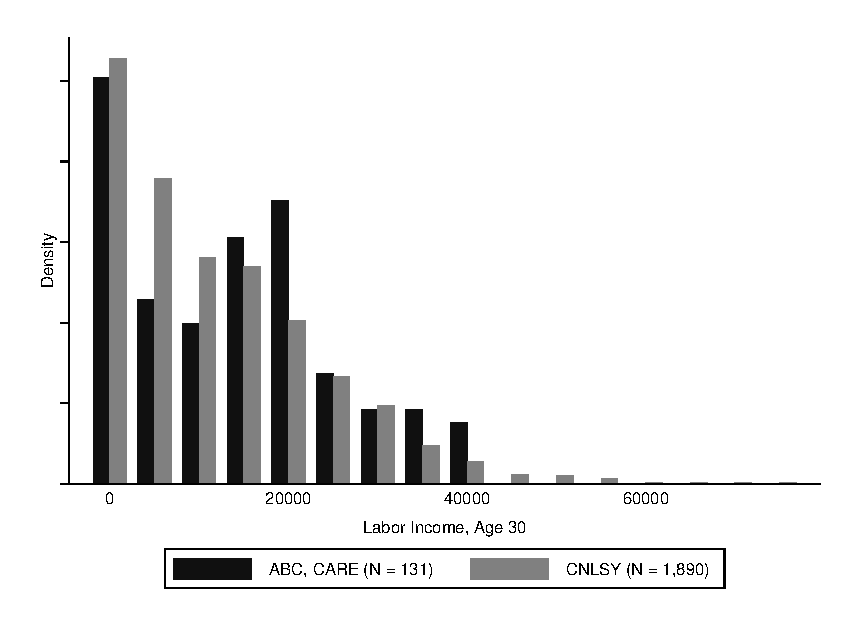
\includegraphics[width=\textwidth]{AppOutput/Methodology/support_inc21.eps}
	\end{subfigure}
	
	\begin{subfigure}[h]{0.8\textwidth}
	\centering
	\caption{Income at Age 30} \label{fig:support_inc30}
	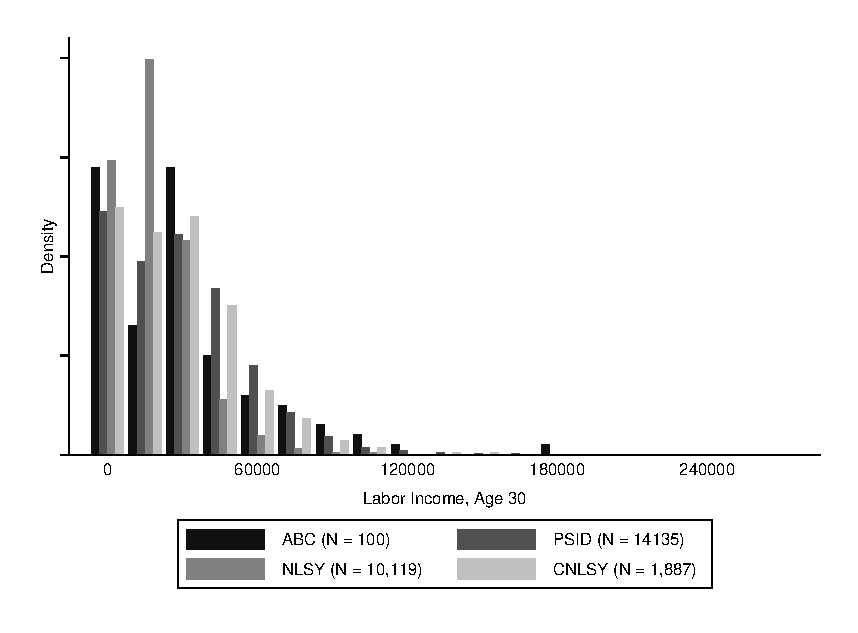
\includegraphics[width=\textwidth]{AppOutput/Methodology/support_inc30.eps}
	\end{subfigure}
\end{figure}




\begin{figure}[H]
	\ContinuedFloat
	\begin{subfigure}[h]{0.8\textwidth}
	\centering
	\caption{Subject's Years of Education} \label{fig:support_educ}
	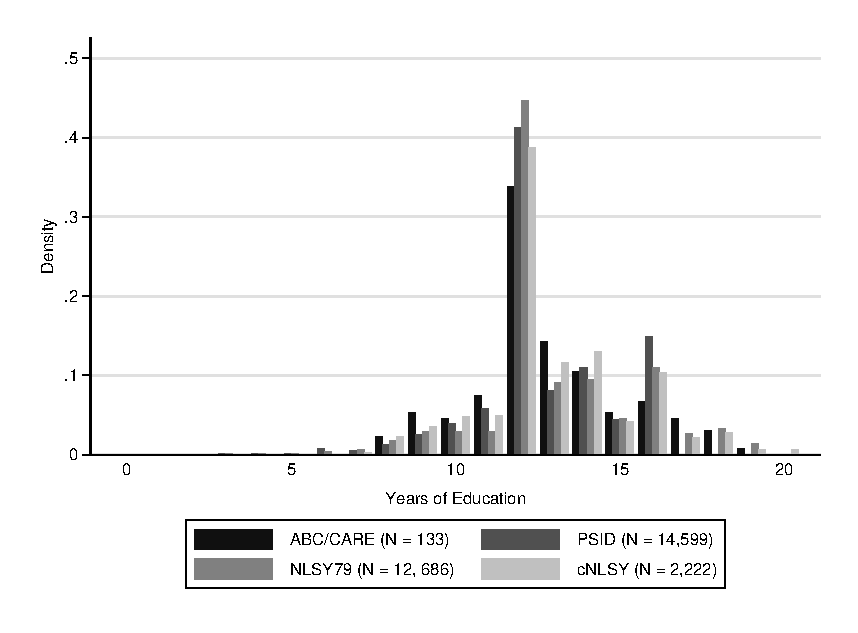
\includegraphics[width=\textwidth]{AppOutput/Methodology/support_educ.eps}
	\end{subfigure}
	
	\begin{subfigure}[h]{0.8\textwidth}
	\centering
	\caption{Mother's Years of Education} \label{fig:support_meduc}
	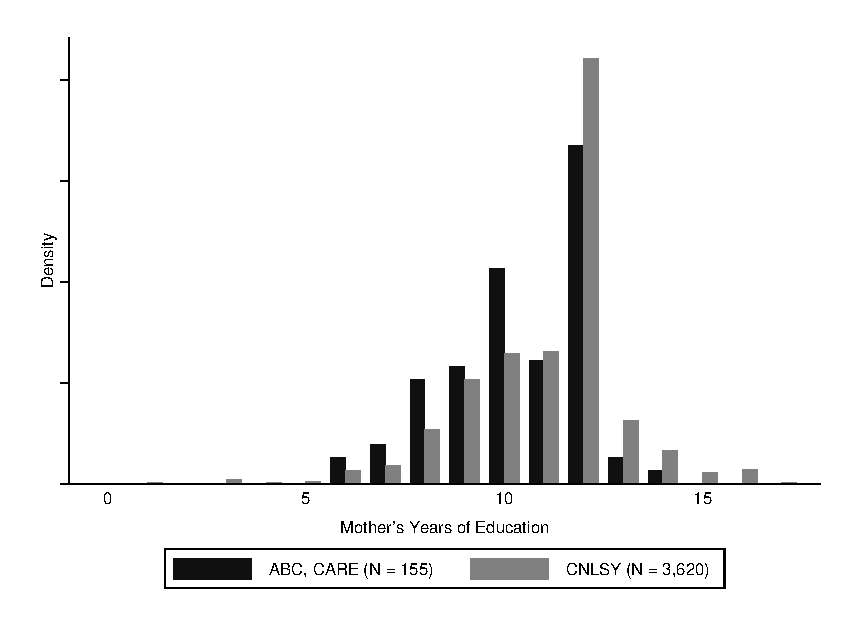
\includegraphics[width=\textwidth]{AppOutput/Methodology/support_momed.eps}
	\end{subfigure}
	
\end{figure}
	
\begin{figure}[H]
	\ContinuedFloat
	\begin{subfigure}[h]{0.8\textwidth}
	\centering
	\caption{Average PIAT Math Scores, Ages 5--7} \label{fig:support_math}
	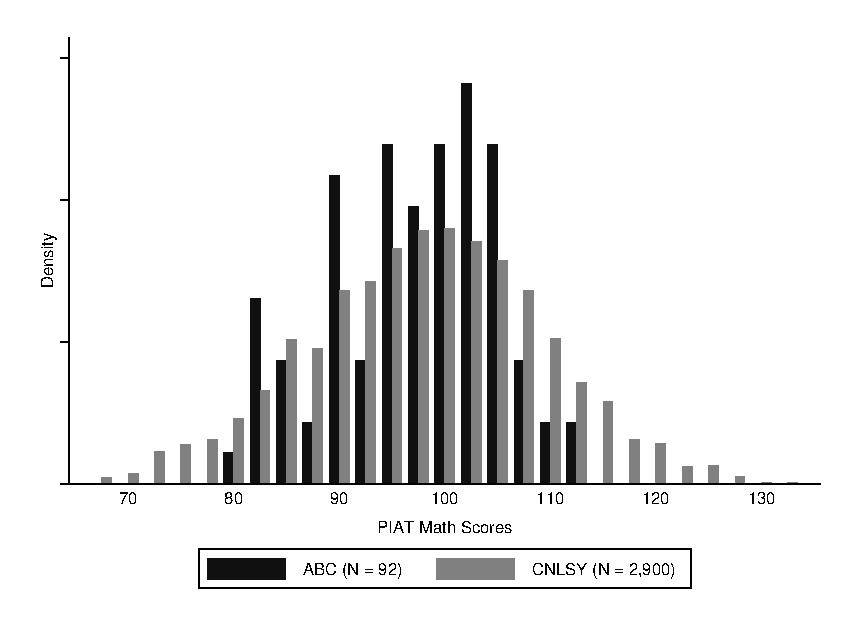
\includegraphics[width=\textwidth]{AppOutput/Methodology/support_math.eps}
	\end{subfigure}
	
	\begin{subfigure}[h]{0.8\textwidth}
	\centering
	\caption{Body Mass Index, Age 34} \label{fig:support_bmi}
	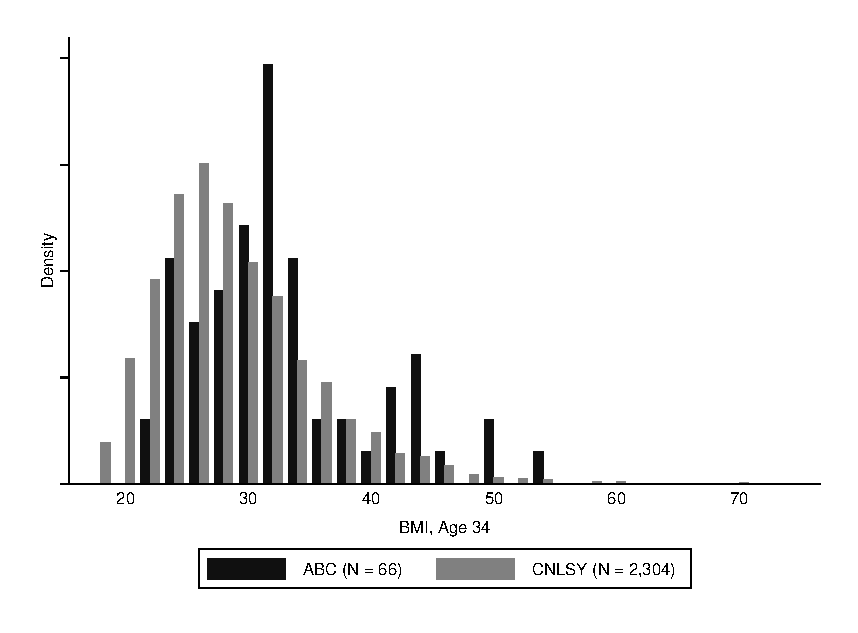
\includegraphics[width=\textwidth]{AppOutput/Methodology/support_bmi.eps}
	\end{subfigure}
	
	\floatfoot{
	\noindent Note: These graphs display the support of ABC, PSID, NLSY, and CNLSY
	for variables we use to project future earnings. PIAT math
	scores are averaged over ages 5--7.
	}
\end{figure}


\noindent Both labor and public-transfer income are interpolated using the exact same methodology, so we restrict
our attention to interpolating labor income. We employ the CNLSY dataset to model labor
income at each age from 22 to 29. We use ordinary least squares and regress the labor income of
CNLSY subjects on background characteristics and early adult outcomes. Variables for background
characteristics consist of an indicator for being  black, mother's education, and sex. Variables
used to interpolate early adult outcomes consist of labor income at ages 21 and 30, years of education at age 30, average
PIAT math scores from ages 5 to 10, and BMI at age 34. We estimate the model on 1,000 bootstrap
resamples of the CNLSY to obtain a measure of prediction error, and denote the vectors of coefficients
\emph{for the outcome variables} by $\beta_{a,s}$, where $a \in \{22, 23, \dots, 29\}$ denotes age, and
$s \in \{1,2,\dots, 1,000\}$ indexes the bootstrap samples. \\

% We impose two restrictions on the CNLSY dataset: one on birth year, and one on income.
% In regard to birth year, we limit the sample to subjects born in between 1978 and 1983. As our
% CNLSY data extends up to 2012, this implies that we use the most recent data from the CNLSY
% where individuals are of age 29 to 34.

% Given the biennial nature of the CNLSY, we observe each subject at either the odd ages or even
% ages. Not only will this reduce the size of our sample on which we fit our prediction model
% at each age, but possibly introduce biases associated with the odd-aged and even-aged cohorts.
% To address this issue, we perform a linear interpolation on the variables in the CNLSY data
% that enter into our prediction model. This allows us to estimate our prediction model on
% all subjects of the CNLSY satisfying our restrictions at every age.

% We further restrict the CNLSY sample to individuals with labor income fewer than
% \$300,000 (USD 2014) at any given year. With the mean labor income in the ABC
% sample being \$12,232.43 at age 21 and \$32,781.96 at age 30 (USD 2014), and the maximum reported
% being \$189,937.50, the cut-off we impose on the auxiliary data is high enough
% so that everyone in the ABC sample is represented, yet low enough to
% exclude high-earning individuals in the auxiliary sample that do not reflect the ABC sample well.

\noindent The outcome variables we use as independent variables to fit the model to the CNLSY data are also
observed in the ABC/CARE data, and we are able to calculate the treatment effects on each of these outcomes
using the procedures described in Appendix \ref{app:method_fullobs} and Appendix \ref{app:method_partialobs}. We
obtain these estimates for 1,-000 bootstrap resamples of both the ABC/CARE data, and denote the vectors of
coefficients by $\gamma_r$, where $r \in \{1,2,\dots,1,000\}$ indexes the bootstrap samples. \\

\noindent To interpolate the treatment effect on subject labor income at age $a$, we take the dot product
of $\beta_{a, s}$ and $\gamma_r$ for all $s,r$ pairs, resulting in 5,625 scalars. We reintroduce
prediction error by first randomly drawing residuals from our fitted model on the auxiliary data and assigning
them to the ABC/CARE subjects. We then take the mean difference of these residuals across treatment and control
groups, and add it to the previously described scalar. We do this for all 5,625scalars. These scalars form the empirical
bootstrap distribution of the treatment effect. Note that
we bypass the estimation of the subjects' actual incomes, for which we are unable to obtain an
unbiased estimate. Instead, we directly obtain an unbiased estimate of the treatment effect. This
method implies that the impacts of the treatment on adult labor income can be expressed through
the observed early-adult outcomes. In this case, the observed early-adult outcomes are labor income at ages 21 and
30, years of education at age 30, average PIAT math scores from ages 5 to 10, and BMI at age 34. Since $\gamma_r$ has
been adjusted to address selection into treatment and attrition in the ABC/CARE data, the bootstrap distribution
is devoid of selection and attrition issues. In addition, the bootstrap distribution captures
the error stemming from the ABC/CARE datasets, and prediction error of the model fitted to the CNLSY dataset.
We take the mean of the empirical bootstrap distribution as our point estimate, and the standard deviation
of the distribution as the standard error. Again, we carry out this procedure for the
pooled, male, and female samples. \\

\noindent To extrapolate labor income, we employ the NLSY79 and PSID datasets. We execute the same estimation
strategy as above, but with a reduced set of control variables in order to limit the number
of dropped cases. Specifically, the set of background variables we control for include an indicator for
being black and gender of the subject. As the NLSY79 and PSID are not as rich as the CNLSY, we also
restrict our outcome variables to years of education at age 30 and subject labor income at age 30. \\
% Similar to the CNLSY, we restrict the PSID to individuals born between 1945 and 1980. As the PSID
% extends until 2013, this means we are using the most recent subsample of individuals aged 30 to 67.
% We do not impose a restriction on birth year on the NLSY as all respondents are aged between 47 and 55
% at the time of the last interview (conducted in 2012). For both the PSID and NLSY, subjects with labor
% income exceeding \$300,000 (USD 2014) are again excluded. Like the CNLSY, because of the biennial
% nature of the PSID and NLSY, we apply a linear interpolation to both data sets.

\noindent We estimate the vectors $\beta_{a, s}$ for $a \in \{31, 32, \dots, 67\}$ and $\gamma_r$, where
$s,r \in \{1,2,\dots,1,000\}$ index the bootstrap samples, and take the dot product of every pair of
$\beta_{a,s}$ and $\gamma_r$ vectors to obtain the empirical bootstrap distribution of the treatment
effect on labor income past age 30. We take the mean of the distribution to be the point estimate,
and the standard deviation of the distribution to be the standard error. \\

%The same procedure is carried out to interpolate and extrapolate transfer income, where we instead
%utilize transfer income as the dependent variable in the regressions on our auxiliary datasets.

\noindent The same procedure is carried out to interpolate public-transfer income, where we instead utilize public-transfer
income as the dependent variable in the regressions on our auxiliary datasets. In the case of
extrapolating public-transfer income from welfare, unemployment benefits, AFDC, and food stamps, we also apply
the same methodology as for labor income. However, in the case of disability insurance, social
security, and supplemental security income, we apply an alternative approach. For these variables, we estimate
the probability each ABC/CARE individual claims each of those benefits at ages 31--67, and multiply those
probabilities by the average annual claims of each type of public transfer reported by the Social
Security Administration in 2014. See Appendix \ref{section:FAM_ABC_impute}
for an explanation of how we estimate these probabilities. For each age, we sum across our estimates of
each type of public transfer received to obtain the total public-transfer income of both ABC/CARE subjects. \\


\paragraph{Health Costs}

\noindent We predict health care costs from age 30 up to age 79, and criminal costs from birth
up to age 50. We then evaluate the predicted outcomes as if observed, and estimate the
treatment effect on those data.\\

\noindent As health outcomes are simulated using a set of variables exhibiting a high rate of attrition, the
predicted health outcomes exhibit an equal rate of attrition. We therefore employ the method described
in Appendix \ref{app:method_partialobs} to estimate the treatment effect on health care costs at
every age from 30 through 79, conditional on survival up to each age. \\

\paragraph{Crime Costs}

\noindent In the case of crime costs, we are able to predict costs for more than 100 individuals in the
sample. We therefore utilize the method described in subsection \ref{app:method_fullobs}
to estimate the treatment effect on the cost of criminal activity at every age from birth until age 50. \\


\begin{table}[H]
\begin{threeparttable}
\caption{Variables Estimated without IPW Adjustment}
\label{table:nonipw}
\centering
% CONTENT CREATED ON SPREADSHEET, TREAT AS A .CSV (TAB DELIMITED)
% CAN BE COPIED INTO A SPREADSHEET PROGRAM (EXCEL, LIBRECALC) FOR EDITING
\begin{tabular}{l l}
\toprule
Variable	&	Age	\\
\midrule			
IQ Standard Score	&	2, 3, 4, 5, 6, 7, 8, 12, 15, 21	\\
PIAT Math Standard Score	&	7	\\
Home Total Score	&	0.5, 1.5, 2.5, 3.5, 4.5, 8	\\
Mother Works	&	2, 3, 4, 5	\\
Biological Mother's Education Level	&	2, 3, 4, 5, 9	\\
Father is Home	&	2, 3, 4, 5	\\
Ever Adopted	&		NA \\
Graduated High School	&	NA	\\
Attended Vocation/Tech/Community College	&	NA	\\
Earned Degree from 4-year College	&	NA	\\
Years of Education	&	30	\\
Works a Job	&	30	\\
Total Felony Arrests	&	Mid-30s	\\
Total Misdemeanor Arrests	&	Mid-30s	\\
Total Years Incarcerated	&	30	\\
Self-reported Health	&	30	\\
Number of Cigarettes Smoked Per Day Last Month	&	30	\\
Number of Days Drank Alcohol Last Month	&	30	\\
Number of Days Binge Drank Alcohol Last Month	&	30	\\
Program Costs	&	0--26	\\
Control Contamination Costs	&	0--26	\\
Education Costs	&	0--26	\\
Medical Expenditure &	8--30	\\
Justice System Costs	&	0--50	\\
Prison Costs	&	0--50	\\
Victimization Costs	&	0--50	\\
\bottomrule			
\end{tabular}
\begin{tablenotes}
\footnotesize
\item Note: The table above lists the variables for which we do not apply IPW when estimating
treatment effects.
\end{tablenotes}
\end{threeparttable}
\end{table}



\begin{sidewaystable}[H]
\caption{Model Selection for Attrition IPW \\ Pooled }
\label{table:ms_attrit_pooled}
\centering
\begin{adjustbox}{max width=\textwidth}
\begin{threeparttable}
% CONTENT CREATED ON SPREADSHEET, TREAT AS A .CSV (TAB DELIMITED)
% CAN BE COPIED INTO A SPREADSHEET PROGRAM (EXCEL, LIBRECALC) FOR EDITING
\scriptsize
\begin{tabular}{l r r l l l}
\toprule											
Partially Observed Outcomes	&	Age	&	N	&	\multicolumn{3}{c}{Variables Used to Produce IPW}	\\
\midrule	
IQ Score 				& 6.5 	& 126   & High Risk Index (HRI)	& APGAR 1 min.	&  Cohort \\
IQ Score 				& 7 	& 118   & High Risk Index (HRI)	& APGAR 5 min.	&  Cohort \\
IQ Score 				& 8 	& 125   & High Risk Index (HRI)	& APGAR 1 min.	&  Cohort \\
\\										
Achievement Score 		& 5.5	& 105 	& High Risk Index (HRI)	& APGAR 1 min.	&  Cohort \\ 
Achievement Score 		& 6		& 124 	& High Risk Index (HRI)	& APGAR 1 min.	&  Cohort \\ 
Achievement Score 		& 6.5	& 89 	& High Risk Index (HRI)	& APGAR 1 min.	&  Cohort \\ 
Achievement Score 		& 7		& 90 	& High Risk Index (HRI)	& APGAR 1 min.	&  Cohort \\ 
Achievement Score 		& 7.5	& 121 	& High Risk Index (HRI)	& APGAR 1 min.	&  Cohort \\ 
Achievement Score 		& 8		& 123 	& High Risk Index (HRI)	& APGAR 1 min.	&  Cohort \\ 
Achievement Score 		& 8.5	& 122 	& High Risk Index (HRI)	& APGAR 5 min.	&  Cohort \\ 
\\
Parental Labor Income	&	1.5	&	112	& Mother's Age at Baseline	& APGAR 1 min.	&  Cohort \\
 Parental Labor Income	&	2.5	&	112	&	Mother's Age at Baseline	& APGAR 1 min.	&  Cohort \\
 Parental Labor Income	&	3.5	&	110	&	Mother's Age at Baseline	& APGAR 1 min.	&  Cohort \\
 Parental Labor Income	&	8	&	87	&	High Risk Index (HRI)	& APGAR 1 min.	&  Cohort \\
 Parental Labor Income	&	12	&	108	&	High Risk Index (HRI)	& APGAR 1 min.	&  Cohort \\
 Parental Labor Income	&	15	&	92	&	APGAR 5 min. & 	Premature at Birth & Number of Siblings, Baseline \\
 Parental Labor Income	&	21	&	73	&	High Risk Index (HRI)	& APGAR 1 min.	&  Cohort \\
\\
HOME Score				& 8		& 	100 & 	High Risk Index (HRI)	& APGAR 1 min.	&  Cohort \\
\\
Father at Home			& 8		& 	116 & 	High Risk Index (HRI)	& APGAR 1 min.	&  Cohort \\
\\
Subject Public Transfer Income	&	21	&	105	& High Risk Index (HRI) & APGAR 1 min. & Cohort \\
 \\
Total Felony Arrests		& Mid-30s	& 115 &	APGAR 1 min. & APGAR 5 min. & Cohort	\\
Total Misdemeanor Arrests	& Mid-30s	& 115 &	APGAR 1 min. & APGAR 5 min. & Cohort	\\
 \\
 Self-reported Health	&	Mid-30s	&	92	&	APGAR 1 min. & APGAR 5 min. & Premature at Birth	\\
 Self-reported Drug User	&	Mid-30s	&	89	&	APGAR 1 min. & APGAR 5 min. & Premature at Birth	\\
 Systolic Blood Pressure (mm Hg)	&	Mid-30s	&	90	&	APGAR 1 min. & Premature at Birth & Number of Siblings, Baseline	\\
 Diastolic Blood Pressure (mm Hg)	&	Mid-30s	 &	90	&	APGAR 1 min. & Premature at Birth & Number of Siblings, Baseline	\\
 Prehypertension, Sys. B.P. $>$ 120 or Dys. B.P. $>$ 80	&	Mid-30s	&	90	&	APGAR 1 min. & Premature at Birth & Number of Siblings, Baseline	\\
 Hypertension, Sys. B.P. $>$ 140 or Dys. B.P. $>$ 90	&	Mid-30s	&	90	&	APGAR 1 min. & Premature at Birth & Number of Siblings, Baseline	\\
 High-Density Lipoprotein (HDL) Cholesterol (mg/dL)	&	Mid-30s	&	93	&	APGAR 1 min. & Premature at Birth & Number of Siblings, Baseline	\\
 Dyslipidemia (HDL $<$ 40 mg/dL)	&	Mid-30s	&	93	&	APGAR 1 min. & Premature at Birth & Number of Siblings, Baseline	\\
 Hemoglobin Level (\%)	&	Mid-30s	&	92	&	APGAR 1 min. & Premature at Birth & Number of Siblings, Baseline	\\
 Prediabetes, Hemoglobin $>$ 5.7\%	&	Mid-30s	&	92	&	APGAR 1 min. & Premature at Birth & Number of Siblings, Baseline	\\
 Diabetes, Hemoglobin $>$ 6.5\%	&	Mid-30s	&	92	&	APGAR 1 min. & Premature at Birth & Number of Siblings, Baseline	\\
 Vitamin D Deficiency ($<$ 20 ng/mL)	&	Mid-30s	&	93	&	APGAR 1 min. & Premature at Birth & Number of Siblings, Baseline	\\
 Measured BMI	&	Mid-30s	&	88	&	APGAR 1 min. & APGAR 5 min. & Premature at Birth \\
 Obesity (BMI $>$ 30)	&	Mid-30s	&	90	&	APGAR 1 min. & APGAR 5 min. & Premature at Birth \\
 Severe Obesity (BMI $>$ 35)	&	Mid-30s	&	91	&	APGAR 1 min. & APGAR 5 min. & Premature at Birth \\
 Waist-hip Ratio	&	Mid-30s	&	84	& APGAR 1 min. & Premature at Birth & Number of Siblings, Baseline \\
 Abdominal Obesity	&	Mid-30s	&	84	& APGAR 1 min. & Premature at Birth & Number of Siblings, Baseline \\
 Framingham Risk Score	&	Mid-30s	&	88	& APGAR 1 min. & Premature at Birth & Number of Siblings, Baseline \\
 Brief Symptom Survey (BSI) Score & Mid-30s & 92 &	APGAR 1 min. & APGAR 5 min. & Premature at Birth	\\
\bottomrule											
\end{tabular}
\begin{tablenotes}
\tiny
\item Note: The table above lists the variables used to generate the
inverse probability weights we use to account for attrition. We estimate a logit model for observing the outcome variable,
controlling for treatment, and three additional covariates depending on the outcome
variable. The additional variables are chosen from a list of covariates possibly affecting
response rates. The set yielding the lowest Akaike Information Criteria value is used to
generate the IPW weights, and are listed in the table above.
\end{tablenotes}
\end{threeparttable}
\end{adjustbox}
\end{sidewaystable}

\begin{sidewaystable}[H]
\caption{Model Selection for Attrition IPW \\ Females }
\label{table:ms_attrit_pooled}
\centering
\begin{adjustbox}{max width=\textwidth}
\begin{threeparttable}
% CONTENT CREATED ON SPREADSHEET, TREAT AS A .CSV (TAB DELIMITED)
% CAN BE COPIED INTO A SPREADSHEET PROGRAM (EXCEL, LIBRECALC) FOR EDITING
\tiny
\begin{tabular}{l r r l l l}
\toprule										
Variable	&	Age	&	Obs.	&	(1)	&	(2)	&	(3)	\\
\midrule											
Parental Labor Income	&	2	&	33	&	Subject Birth Year	&	Mother Works, age 5	&	Father works before pregnancy	\\
Parental Labor Income	&	3	&	33	&	Subject Birth Year	&	Mother Works, age 5	&	Father works before pregnancy	\\
Parental Labor Income	&	4	&	31	&	Subject Birth Year	&	Father works before pregnancy	&	Siblings in Household, age 5	\\
Parental Labor Income	&	5	&	44	&	Mother Works before Pregnant	&	Mother Works, age 5	&	Father works before pregnancy	\\
Parental Labor Income	&	9	&	40	&	Mother Works, age 5	&	HRI 2: No Maternal Relatives	&	Father works before pregnancy	\\
Parental Labor Income	&	12	&	45	&	Subject Birth Year	&	Mother Works, age 5	&	Father works before pregnancy	\\
Parental Labor Income	&	15	&	47	&	Mother Works, age 5	&	HRI 2: No Maternal Relatives	&	Father works before pregnancy	\\
\\
Subject Labor Income	&	21	&	51	&	Mother's WAIS Performance IQ	&	Mother's Age at entry	&	ASR t-score: Attention Deficit and Hyperactivity	\\
Subject Labor Income	&	30	&	53	&	HRI 10: Other special circumstances	&	ASR t-score: Substance Abuse	&	Years of Education	\\
Subject Public Transfer Income	&	21	&	49	&	Mother's WAIS Comprehension	&	Number of cigarettes smoked per day	&	ASR t-score: Attention Deficit and Hyperactivity	\\
Subject Public Transfer Income	&	30	&	53	&	HRI 10: Other special circumstances	&	ASR t-score: Substance Abuse	&	Years of Education	\\
\\
Self-reported Health	&	Mid-30s	&	40	&	Length at birth	&	ASR t-score: Substance Abuse	&	Years of Education	\\
Self-reported Drug User	&	Mid-30s	&	40	&	Length at birth	&	ASR t-score: Substance Abuse	&	Years of Education	\\
Systolic Blood Pressure (mm Hg)	&	Mid-30s	&	40	&	Length at birth	&	ASR t-score: Substance Abuse	&	Years of Education	\\
Diastolic Blood Pressure (mm Hg)	&	Mid-30s	&	40	&	Length at birth	&	ASR t-score: Substance Abuse	&	Years of Education	\\
Prehypertension, Sys. B.P. $>$ 120 or Dys. B.P. $>$ 80	&	Mid-30s	&	40	&	Length at birth	&	ASR t-score: Substance Abuse	&	Years of Education	\\
Hypertension, Sys. B.P. $>$ 140 or Dys. B.P. $>$ 90	&	Mid-30s	&	40	&	Length at birth	&	ASR t-score: Substance Abuse	&	Years of Education	\\
High-Density Lipoprotein (HDL) Cholesterol (mg/dL)	&	Mid-30s	&	40	&	Length at birth	&	ASR t-score: Substance Abuse	&	Years of Education	\\
Dyslipidemia (HDL $<$ 40 mg/dL)	&	Mid-30s	&	40	&	Length at birth	&	ASR t-score: Substance Abuse	&	Years of Education	\\
Hemoglobin Level (\%)	&	Mid-30s	&	39	&	Length at birth	&	ASR t-score: Substance Abuse	&	Years of Education	\\
Prediabetes, Hemoglobin $>$ 5.7\%	&	Mid-30s	&	39	&	Length at birth	&	ASR t-score: Substance Abuse	&	Years of Education	\\
Diabetes, Hemoglobin $>$ 6.5\%	&	Mid-30s	&	39	&	Length at birth	&	ASR t-score: Substance Abuse	&	Years of Education	\\
Vitamin D Deficiency ($<$ 20 ng/mL)	&	Mid-30s	&	40	&	Length at birth	&	ASR t-score: Substance Abuse	&	Years of Education	\\
Measured BMI	&	Mid-30s	&	40	&	Length at birth	&	ASR t-score: Substance Abuse	&	Years of Education	\\
Obesity (BMI $>$ 30)	&	Mid-30s	&	40	&	Length at birth	&	ASR t-score: Substance Abuse	&	Years of Education	\\
Severe Obesity (BMI $>$ 35)	&	Mid-30s	&	40	&	Length at birth	&	ASR t-score: Substance Abuse	&	Years of Education	\\
Waist-hip Ratio	&	Mid-30s	&	37	&	Length at birth	&	ASR t-score: Substance Abuse	&	Years of Education	\\
Abdominal Obesity	&	Mid-30s	&	37	&	Length at birth	&	ASR t-score: Substance Abuse	&	Years of Education	\\
Framingham Risk Score	&	Mid-30s	&	39	&	Length at birth	&	ASR t-score: Substance Abuse	&	Years of Education	\\
\bottomrule																																	
\end{tabular}
\begin{tablenotes}
\tiny
\item Note: The table above lists the variables used to generate the
inverse probability weights we use to account for attrition. We estimate a logit model for observing the outcome variable,
controlling for treatment, and three additional covariates depending on the outcome
variable. The additional variables are chosen from a list of covariates possibly affecting
response rates. The set yielding the lowest Akaike Information Criteria value is used to
generate the IPW weights, and are listed in the table above.
\end{tablenotes}
\end{threeparttable}
\end{adjustbox}
\end{sidewaystable}



\begin{sidewaystable}[H]
\caption{Model Selection for Attrition IPW \\ Males }
\label{table:ms_attrit_pooled}
\centering
\begin{adjustbox}{max width=\textwidth}
\begin{threeparttable}
% CONTENT CREATED ON SPREADSHEET, TREAT AS A .CSV (TAB DELIMITED)
% CAN BE COPIED INTO A SPREADSHEET PROGRAM (EXCEL, LIBRECALC) FOR EDITING
\tiny
\begin{tabular}{l r r l l l}
\hline\hline											
Variable	&	Age	&	Obs.	&	(1)	&	(2)	&	(3)	\\
\hline											
Parent Labor Income	&	2	&	39	&	Subject Birth Year	&	Mother Works, age 3	&	Siblings in Household, age 3	\\
Parent Labor Income	&	3	&	39	&	Subject Birth Year	&	Mother Works, age 3	&	Father works before pregnancy	\\
Parent Labor Income	&	4	&	38	&	Subject Birth Year	&	Mother Works, age 4	&	Siblings in Household, age 3	\\
Parent Labor Income	&	5	&	42	&	Mother Works, age 3	&	Mother Works, age 4	&	Siblings in Household, age 5	\\
Parent Labor Income	&	9	&	42	&	Mother Works, age 3	&	Father home, age 5	&	Siblings in Household, age 5	\\
Parent Labor Income	&	12	&	46	&	Subject Birth Year	&	Mother Works, age 4	&	Father home, age 5	\\
Parent Labor Income	&	15	&	43	&	Mother Works, age 4	&	Father works before pregnancy	&	Siblings in Household, age 5	\\
\\
Subject Labor Income	&	21	&	45	&	HRI 10: Other special circumstances	&	Gestational Age $\leq$ 36	&	ASR t-score: Substance Abuse	\\
Subject Labor Income	&	30	&	47	&	Father's Age at entry	&	Mother Married at entry	&	ASR t-score: Substance Abuse	\\
Subject Public Transfer Income	&	21	&	48	&	Father's Age at entry	&	Gestational Age $\leq$ 36	&	Years of Education	\\
Subject Public Transfer Income	&	30	&	48	&	Mother's WAIS Performance IQ	&	ASR t-score: Antisocial Personality Problems	&	Had physical exam for illness in last 2 years	\\
\\
Self-reported Health	&	Mid-30s	&	30	&	HRI 2: No Maternal Relatives	&	ASR t-score: Substance Abuse	&	ASR t-score: Antisocial Personality Problems	\\
Self-reported Drug User	&	Mid-30s	&	27	&	Gestational Age $\leq$ 36	&	ASR t-score: Substance Abuse	&	Had physical exam for illness in last 2 years	\\
Systolic Blood Pressure (mm Hg)	&	Mid-30s	&	28	&	Gestational Age $\leq$ 36	&	ASR t-score: Substance Abuse	&	Had physical exam for illness in last 2 years	\\
Diastolic Blood Pressure (mm Hg)	&	Mid-30s	&	28	&	Gestational Age $\leq$ 36	&	ASR t-score: Substance Abuse	&	Had physical exam for illness in last 2 years	\\
Prehypertension, Sys. B.P. $>$ 120 or Dys. B.P. $>$ 80	&	Mid-30s	&	28	&	Gestational Age $\leq$ 36	&	ASR t-score: Substance Abuse	&	Had physical exam for illness in last 2 years	\\
Hypertension, Sys. B.P. $>$ 140 or Dys. B.P. $>$ 90	&	Mid-30s	&	28	&	Gestational Age $\leq$ 36	&	ASR t-score: Substance Abuse	&	Had physical exam for illness in last 2 years	\\
High-Density Lipoprotein (HDL) Cholesterol (mg/dL)	&	Mid-30s	&	31	&	Gestational Age $\leq$ 36	&	ASR t-score: Substance Abuse	&	Had physical exam for illness in last 2 years	\\
Dyslipidemia (HDL $<$ 40 mg/dL)	&	Mid-30s	&	31	&	Gestational Age $\leq$ 36	&	ASR t-score: Substance Abuse	&	Had physical exam for illness in last 2 years	\\
Hemoglobin Level (\%)	&	Mid-30s	&	31	&	Gestational Age $\leq$ 36	&	ASR t-score: Substance Abuse	&	Had physical exam for illness in last 2 years	\\
Prediabetes, Hemoglobin $>$ 5.7\%	&	Mid-30s	&	31	&	Gestational Age $\leq$ 36	&	ASR t-score: Substance Abuse	&	Had physical exam for illness in last 2 years	\\
Diabetes, Hemoglobin $>$ 6.5\%	&	Mid-30s	&	31	&	Gestational Age $\leq$ 36	&	ASR t-score: Substance Abuse	&	Had physical exam for illness in last 2 years	\\
Vitamin D Deficiency ($<$ 20 ng/mL)	&	Mid-30s	&	31	&	Gestational Age $\leq$ 36	&	ASR t-score: Substance Abuse	&	Had physical exam for illness in last 2 years	\\
Measured BMI	&	Mid-30s	&	26	&	Gestational Age $\leq$ 36	&	ASR t-score: Substance Abuse	&	Had physical exam for illness in last 2 years	\\
Obesity (BMI $>$ 30)	&	Mid-30s	&	28	&	Father works before pregnancy	&	ASR t-score: Substance Abuse	&	ASR t-score: Attention Deficit and Hyperactivity	\\
Severe Obesity (BMI $>$ 35)	&	Mid-30s	&	29	&	HRI 2: No Maternal Relatives	&	Mother's WAIS Comprehension	&	Number of times smoked marijuana	\\
Waist-hip Ratio	&	Mid-30s	&	25	&	Gestational Age $\leq$ 36	&	ASR t-score: Substance Abuse	&	Had physical exam for illness in last 2 years	\\
Abdominal Obesity	&	Mid-30s	&	25	&	Gestational Age $\leq$ 36	&	ASR t-score: Substance Abuse	&	Had physical exam for illness in last 2 years	\\
Framingham Risk Score	&	Mid-30s	&	27	&	Gestational Age $\leq$ 36	&	ASR t-score: Substance Abuse	&	Had physical exam for illness in last 2 years	\\
\hline\hline																							
\end{tabular}
\begin{tablenotes}
\tiny
\item Note: The table above lists the variables used to generate the
inverse probability weights we use to account for attrition. We estimate a logit model for observing the outcome variable,
controlling for treatment, and three additional covariates depending on the outcome
variable. The additional variables are chosen from a list of covariates possibly affecting
response rates. The set yielding the lowest Akaike Information Criteria value is used to
generate the IPW weights, and are listed in the table above.
\end{tablenotes}
\end{threeparttable}
\end{adjustbox}
\end{sidewaystable}

\subsection{Internal Rate of Return}
\label{app:method_irr}

\noindent To estimate the internal rate of return, we must solve for $\rho$ in the equation below,

\begin{align}
\sum_{t=0}^T \frac{ \mathbb{E} (B_t - C_t)}{(1+\rho)^t} = 0,
\end{align}

\noindent where we let $T = 79$, define $B_t$ and $C_t$ to be the total benefits and costs of the
program at time $t$, and define $\mathbb{E}$ to be the sample mean. \\

\noindent All outcomes of the parents and subjects that we observe as having been affected by the program
are treated as benefits. For this to make sense, we reverse the sign of the monetized effect of the program
on specific outcomes. Costs of ABC/CARE consist only of the initial program costs from ages 0 to 5.
Table \ref{table:bc_comp} provides a full list of the benefits and costs of ABC. \\

\noindent We take the sum of the treatment effects on each component of the benefits to
be the total benefit, $B_t$, of the ABC/CARE program (see Appendix \ref{app:method_identify} on how
we estimate these treatment effects). This includes parental income, subject labor income, and QALYs
(quality-adjusted life years).
Treatment effects on costs borne by the subject or society have their signs
reversed and are included as benefits. We do this for subject public-transfer income,
education costs, crime costs,
control contamination costs, and health costs. To account for deadweight loss, we
impose a marginal welfare cost of 50\% by multiplying public costs by a factor of
$1.5$.\footnote{There is no clear consensus on the marginal welfare cost of tax revenue. However,
most researchers estimate the welfare cost per tax dollar to be between \$0.30 and \$0.50. See
\citet{Feldstein_1999_REStat}, \citet{Heckman_Smith_1998_evaluating}, and \citet{Browning_1987_AER}.} Public costs include education costs up until age 17, jail costs, justice system costs, Medicare costs,
Medicaid costs, disability insurance claims, social security claims, and supplemental security
income. \\

\noindent Having constructed our cash flow, $\mathbb{E} (B_t - C_t)$, solving for $\rho$
reduces to an algebraic exercise. \\

\noindent As described in Appendix \ref{app:method_identify}, we estimate the treatment effect on each
component of the benefits and costs at time $t$ for the pooled, male, and
female samples. We do this for 1,000 bootstrap resamples of the original ABC/CARE data.
In the case of health costs and subject income, for which we employ auxiliary datasets to
estimate the treatment effects, we also obtain 1,000 bootstrap estimates from the auxiliary data
for every ABC/CARE bootstrap resample, resulting in a total of 1,000,000 estimates.
By reusing each bootstrap estimate of the treatment effect on outcomes that do not require any auxiliary data
set 1,000 times, we obtain a total of 1,000,000 estimates of the cash flow.
We estimate the IRR on each of those cash flows.
This is how we form our empirical bootstrap distribution of the IRR for the pooled, male, and female samples.
We take the mean of the distributions to be the point estimates, and we take the standard deviations
to be the standard errors. To construct the 80\% confidence intervals, we take the 10\textsuperscript{th}
and 90\textsuperscript{th} quantiles of each bootstrap distribution. \\

\noindent{\textbf{[JJH: What is the basis for the 0.5 in public-transfer income? Why the 1.5?]}}

\begin{table}[H]
\begin{threeparttable}
\caption{Components of Benefits and Costs}
\label{table:bc_comp}
\centering
\begin{tabular}{l c c}
\toprule			
Variable & Sign Reversed	& Welfare Cost \\
	&		& Factor \\
\midrule
\textbf{Benefits} 	\\			
\quad Parent Income			& \\
\quad Subject QALY			& \\
\quad Subject Labor Income	& \\
\quad Subject Public-transfer Income	& $\checkmark$	& 0.5 \\
\quad Medicare Costs			& $\checkmark$	& 1.5 \\
\quad Medicaid Costs			& $\checkmark$	& 1.5 \\
\quad Out-of-pocket Medical Costs	& $\checkmark$ \\
\quad Miscellaneous Medical Costs	& $\checkmark$ \\
\quad Disability Insurance Claim	& $\checkmark$	&	1.5 \\
\quad Social Security Claim	& $\checkmark$	&	1.5 \\
\quad Supplemental Security Claim	& $\checkmark$	&	1.5 \\
\quad Control Substitution Costs	& $\checkmark$	& \\
\quad Education Costs			& $\checkmark$	& 1.5* \\
\quad Justice System Costs	& $\checkmark$	& 1.5 \\
\quad Prison Costs			& $\checkmark$	& 1.5 \\
\quad Victimization Costs		& $\checkmark$	& \\
\textbf{Costs} 	\\			
\quad Program Costs			& \\
\bottomrule			
\end{tabular}
\begin{tablenotes}
\tiny
\item Note: The table lists the components of the costs and benefits of ABC/CARE.
In order for some components to be categorized as benefits, we reversed the sign
of the treatment effect. *Only education costs up until age 18 are multiplied by 1.5 to account for welfare costs.
\end{tablenotes}
\end{threeparttable}
\end{table}


% We let $T = 79$. In Appendix \ref{app:method_identify}
% we explain how we can estimate the summand of the numerator at every period $t$, which
% can be expressed as $\mathbf{E}(B_t) -  \mathbf{E}(C_t)$. Thus, solving for $\rho$
% reduces to an algebraic exercise.



% To construct our cash flow, we subtract the costs from benefits to create a single stream.
% We define `cost' to include only the program costs of ABC, and define
% `benefits' to include all treatment effects of the program. This includes
% the treatment effects on parent income, subject labor income, and QALY
% (quality adjusted life years).\footnote{QALYs are measured on a scale of 0 to 1, with 1 being a
% year of perfect health. We follow \textbf{[CITATION]} and value a QALY of 1 to be
% \$150,000, and a QALY of 0 to be \$0. The dollar value of that year relates linearly to the QALY.}
% Treatment effects on costs borne by the subject or society have their signs
% reversed and are included as benefits. We do this for subject transfer income,
% education costs, jail costs, justice system costs, victimization costs,
% control contamination costs, and medical costs. To account for deadweight loss, we
% impose a marginal welfare cost of 50\% by multiplying public costs by a factor of
% $1.5$.\footnote{There is no clear consensus on the marginal welfare cost of tax revenue. However,
% most researchers estimate the welfare cost per tax dollar is between \$0.30--0.50. See
% \citet{feldstein1999tax, heckman1998evaluating, browning1987marginal}.} This
% includes education cost up until age 17, jail costs, justice system costs, Medicare costs,
% and Medicaid costs. For the same reason, we multiply transfer income by a factor of 0.5.

% For each period $t \in \{1, 2, \dots, 79\}$, we sum our estimates of the benefits, and
% subtract our estimates of the costs from that sum. This provides us an estimate of
% $\mathbf{E}(B_t) -  \mathbf{E}(C_t) = \mathbf{E} (B_t - C_t)$. We then solve for
% $\rho$ using numerical analysis.

% In your methodlogy you describe costs and benefits differnetly....
% To construct our cash flow, we sum the costs and benefits from the program into a single stream.
% We define `cost' to include only the cost of implementing ABC. On the other hand,
% we broadly define `benefits' to include all treatment effects of the program. This includes
% the treatment effects on parent income, subject labor income, and QALY
% (quality adjusted life years).\footnote{QALYs are measured on a scale of 0 to 1, with 1 being a
% year of perfect health. We follow \textbf{[CITATION]} and value a QALY of 1 to be
% \$150,000, and a QALY of 0 to be \$0. The dollar value of that year relates linearly to the QALY.}
% Treatment effects on outcomes generally considered to be costs have their signs reversed in
% order to convert them into benefits. We do this for subject transfer income,
% education costs, jail costs, justice system costs, victimization costs,
% control contamination costs, and medical costs. To account for deadweight loss, we
% impose a marginal welfare cost of 50\% by multiplying public costs by a factor of
% $1.5$.\footnote{There is no clear consensus on the marginal welfare cost of tax revenue. However,
% most researchers estimate the welfare cost per tax dollar is between \$0.30--0.50. See
% \citet{feldstein1999tax, heckman1998evaluating, browning1987marginal}.} This
% includes education cost up until age 17, jail costs, justice system costs, Medicare costs,
% and Medicaid costs. For the same reason, we multiply transfer income by a factor of 0.5.


\subsection{Computing the Benefit/cost Ratio}
\label{app:method_cbratio}

\noindent The benefit/cost ratio can be expressed as,

\begin{align}
\mathbb{E} \left( \frac{ \sum_{t=0}^T B_t}{\sum_{t=0}^T C_t} \right),
\end{align}

\noindent where we let $T = 79$, define $B_t$ and $C_t$ to be the total benefits and costs of the
program at time $t$, and define $\mathbb{E}$ to be the sample mean. See Table \ref{table:bc_comp} for a detailed list of the components
to the benefits and costs of ABC/CARE . We take the sum of the treatment effects on each component
of the benefits to be the total benefits of the ABC/CARE programs (see Appendix~\ref{app:method_identify} on how we estimate these treatment effects). \\

\noindent To account for deadweight loss, we assume a marginal welfare cost of 50\% by multiplying
public costs components by a factor of $1.5$. For the same reason, we multiply public-transfer
income by a factor of 0.5 \textbf{[JJH: Why? What principle?]}. We discount each component of the benefits and costs
by 3\% every year to obtain their net present value at birth. We then sum up the discounted
components of the benefits and find the ratio with the discounted costs. \\

\noindent As described in Appendix \ref{app:method_identify}, we estimate the treatment effect on each
component of the benefits and costs at time $t$ for the pooled, male, and
female samples. We do this for 1,000 bootstrap resamples of the original ABC/CARE data.
In the case of health costs and subject income, for which we employ auxiliary datasets to
estimate the treatment effects, we also obtain 1,000 bootstrap estimates from the auxiliary data
for every ABC/CARE bootstrap resample, resulting in a total of 1,000,000 estimates.
By reusing each bootstrap estimate of the treatment effect on outcomes that do not require any auxiliary data
set 1,000 times, we obtain a total of 1,000,000 estimates of the costs stream and benefits stream.
We estimate the benefit/cost ratio for each of those streams.
This is how we form our empirical bootstrap distribution of the benefit/cost ratio for the pooled, male, and female samples.
We take the mean of the distributions to be the point estimates, and we take the standard deviations
to be the standard errors. To construct the 80\% confidence intervals, we take the 10\textsuperscript{th}
and 90\textsuperscript{th} quantiles of each bootstrap distribution.






\setcounter{figure}{0}  \renewcommand{\thefigure}{I.\arabic{figure}}
\setcounter{table}{0}   \renewcommand{\thetable}{I.\arabic{table}}
\section[Program Costs of ABC/CARE]{Program Costs\footnote{Sylvi Kuperman greatly assisted us in preparing this section of the appendix.}} \label{app:programcosts}

\noindent In this appendix, we document the sources informing our programs' costs calculation in Section~\ref{section:programscosts}. We use a battery of primary sources obtained in the Archives of the University of North Carolina at Chapel Hill---Records of the Office of the Vice Chancellor \citet{UNC-Archives_Health-Affairs}. Figure~\ref{figure:who} exemplifies one of these sources, in which the monthly cost of treatment per child for the year 1977 is categorized by source of funding.

\begin{center}
\begin{figure}[H] 
\caption{Primary-source Document Costs, Example}
\label{figure:who}
\centering
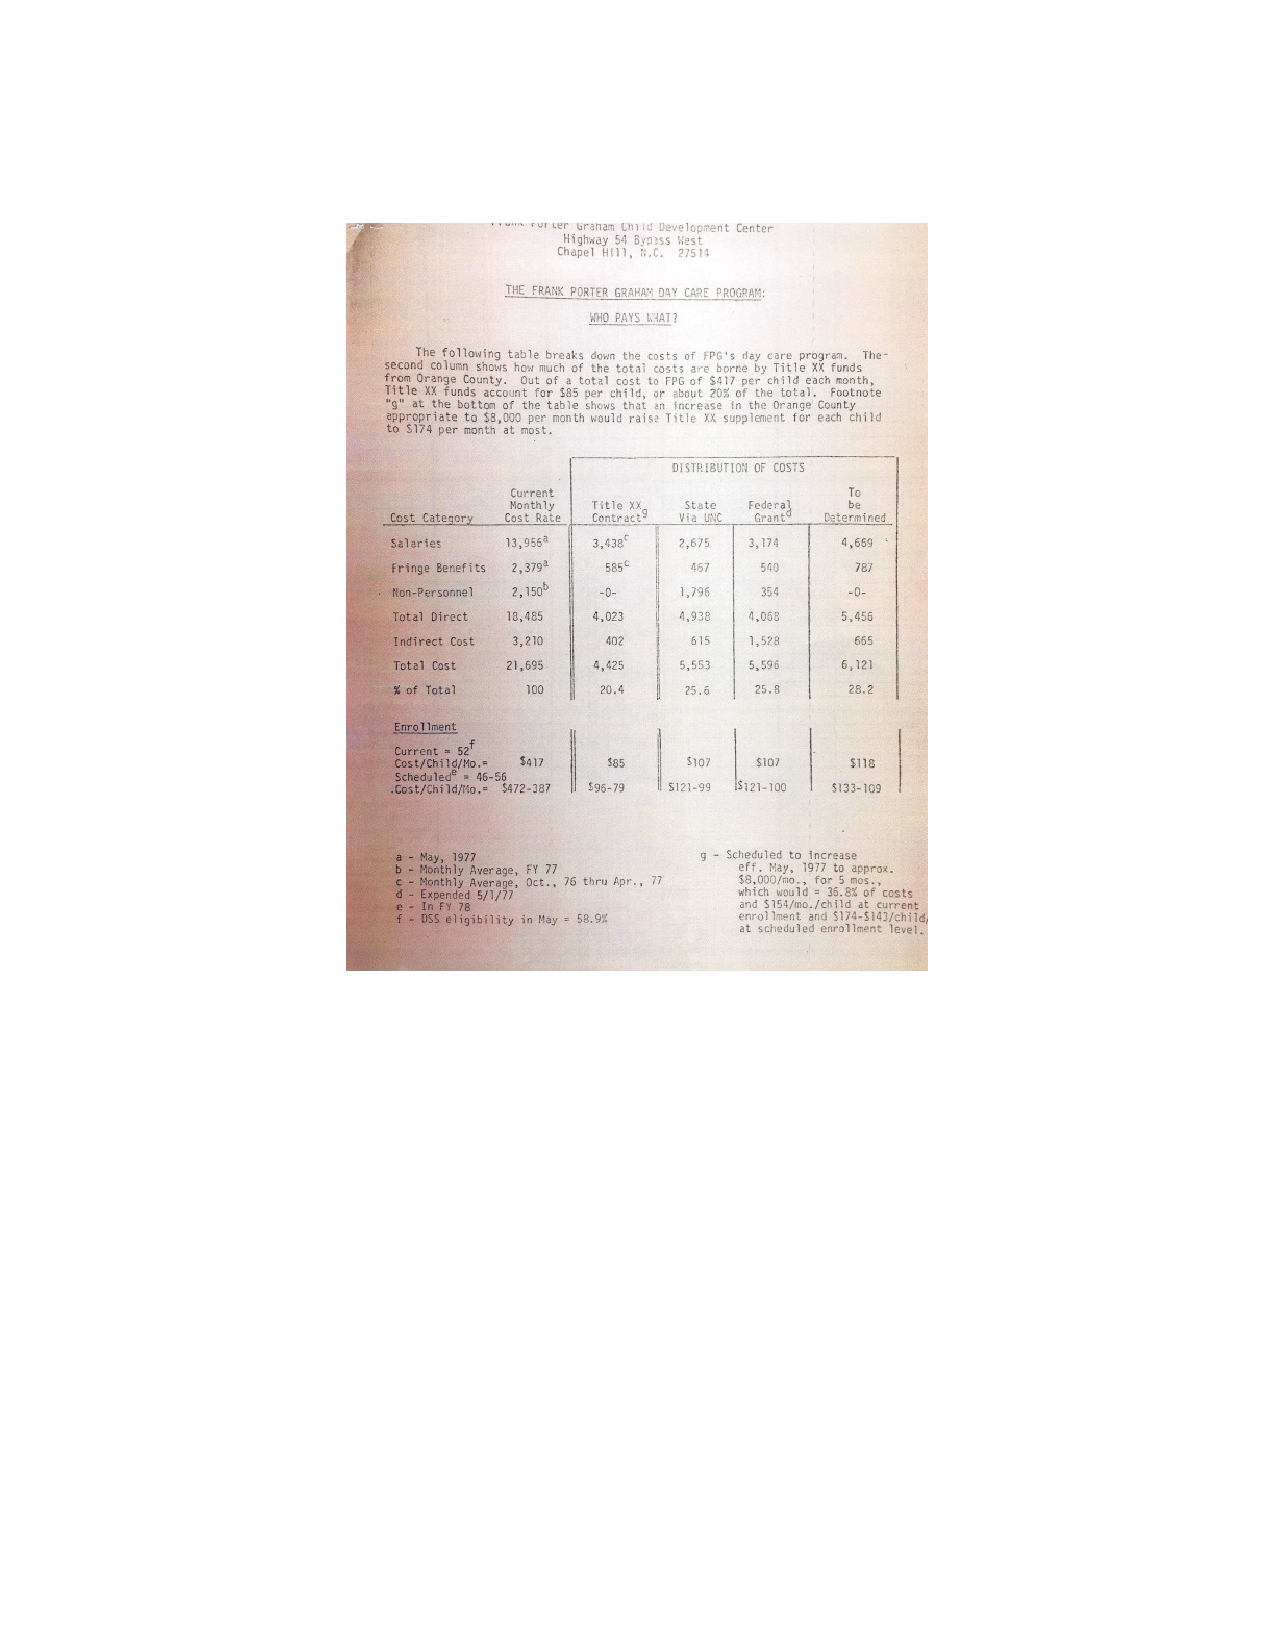
\includegraphics[width=.9\columnwidth]{AppOutput/Program/UNC-costs.pdf}
\floatfoot{
\footnotesize
Note: This figure is a photograph exemplifying the primary-source document we use in the calculation of the programs' cost. It was obtained in the University of North Carolina at Chapel Hill---Records of the Office of the Vice Chancellor}
\end{figure}
\end{center}

\noindent Figure~\ref{figure:wages} is another of our sources and it is the base of our calculation of personnel costs.

\begin{center}
\begin{figure}[H] 
\caption{Primary-source Document Costs, Personnel Wages}
\label{figure:wages}
\centering

\includegraphics[width=.9\columnwidth]{AppOutput/Program/UNC-costs_budget.pdf}
\floatfoot{
\footnotesize
Note: This figure is a photograph provides the estimates for the personnel wages we use. It was obtained in the University of North Carolina at Chapel Hill---Records of the Office of the Vice Chancellor}
\end{figure}
\end{center}

\noindent Interviews with the programs' staff \citet{projectcare2014interviews,abc2014-2015interviews}, inform us about additional costs of the programs. An example is the salary of a social worker, who is not part of some of the of the costs estimates reported before but was part of the staff implementing treatment. These interviews are available upon request.\\ 

\noindent Finally, a valuable source is a report written by the program staff \citet{FPG_1979_Progress-Report}. As we note in Section~\ref{section:programscosts}, this report produced an estimate of the cost in a completely independent way, although perhaps using a the same or similar primary sources. Our calculation of the costs comes very close to those in \citet{FPG_1979_Progress-Report}. \\

\noindent We summarize the yearly program costs of ABC/CARE in Table~\ref{tab:totalcosts}. \\

\begin{table}[H]
\centering
\begin{threeparttable}
\caption{Yearly Program Costs, ABC/CARE} \label{tab:totalcosts}
\footnotesize
\begin{tabular}{lc} \toprule
\multicolumn{1}{c}{Item} & Yearly Cost in 2014 USD \\ \midrule
1 Program Director & $60,935$ \\ 
1 Social Worker      &  $35,869$ \\ 
3 Lead Teachers and 2 Teachers Aides (Nursery)  & $204,457$ \\
4 Lead Teachers and 4 Teacher Aides  (Toddlers) & $305,181$ \\ 
2 Teaching Support Staff & $53,341$ \\ 
1 Secretary & $32,973$ \\ 
1 Clerk        & $32,537$ \\ 
Workers' Fringe Benefits & $124,935$ \\ 
Other & $4, 891$ \\ \\ \midrule 
Total  & $962,726$ \\ 
Total per Subject & $18,514$ \\ \bottomrule
\end{tabular}
\begin{tablenotes}
\footnotesize
\item Note: This table summarizes the yearly costs for ABC/CARE. They are based on primary-source documentation describing ABC. We assume that the costs for ABC and CARE were the same based on conversations with programs' staff \citep{projectcare2014interviews,abc2014-2015interviews}. \\
\end{tablenotes}
\end{threeparttable}
\end{table}

\setcounter{figure}{0}  \renewcommand{\thefigure}{J.\arabic{figure}}
\setcounter{table}{0}   \renewcommand{\thetable}{J.\arabic{table}}
\section{Costs of Education} \label{appendix:education}

\noindent We account for short- and long-term components of educational costs. The short-term components include savings due to reductions in special education and grade retention. The long-term components include the type and level of the highest educational attainment at age 30. We do not calculate costs of education beyond age 30 because we do not have data on the subjects' later educational attainment. Instead of forming a projection of future education costs, we do not add further modeling uncertainty through this component and document that, at the national level, education beyond age 30 increases marginally. To document this, we use the Panel Study of Income Dynamics (PSID) for a representative sample of individuals born between 1972 and 1982. \\

\noindent To estimate the costs of additional schooling, we combine various sources. Table \ref{tab:yearlyedu}  describes the yearly cost of education at every level and the age and duration for which these costs are incurred. We apply these costs additively up to the highest level of educational attainment by age 30. Pooling males and females, the treatment groups had on average higher attainment and incurred a greater cost of education. To find the present value of the difference between the treatment and control groups, we first order educational attainment per Table \ref{tab:yearlyedu}. We find a difference between the average educational attainment of the treatment groups (finish community college) and the average educational attainment of the control groups (start community college). This can be represented as a cost that is \$12,586 higher for the treatment groups than for the control groups, as in Table \ref{tab:yearlyedu}. The effect of the program on the educational attainment of females, however, is much greater than the effect on that of males.

\subsection{Measuring Lifetime Educational Attainment}

\noindent Follow-up data on educational attainment were collected for ABC/CARE subjects up to age 30, on average. This may not necessarily be an accurate measure of lifetime educational attainment. Thus, we perform an exercise using nationally representative data from the Panel Study of Income Dynamics (PSID) to assess educational attainment after age 30. We find only one additional year of schooling for individuals between the ages of 40 and 60. \\

\subsection{Cost of Education}
\noindent We apply the costs described in Table \ref{tab:yearlyedu} to subjects' educational attainment at age 30 to calculate the public and private costs of lifetime educational attainment. Costs up to high school are assumed to be public costs. \\

\begin{table}[H]
\caption{Yearly Individual Education Costs} \label{tab:yearlyedu}
\centering
\begin{adjustbox}{max width=\textwidth}
\begin{threeparttable}
\footnotesize
\begin{tabular}{C{3.5cm} C{1.5cm} C{1.5cm} C{2cm} C{6.5cm}}
\toprule
Schooling level & Ages & Duration (Years) & Yearly Cost &Attainment \& Notes\\ \midrule
K-11 & 6-16 & 10 &   \$9,113  & All subjects. Only 1 control individual dropped out before completing 9th grade; we assume completion up to 8th grade. \\
Grade 12 & 17-18 & 2 &  \$9,113  & Counted only for subjects who completed high school, 29:38 (control:treatment).\\ \\
GED (Started) & 19 & .5 &  \$155& GED is considered a one year program. No subjects identified as having starting a GED program without finishing.\\ \\
GED (Completed) & 19 & 1 & \$155 & 8:6 (control:treatment).\\ \\
Vocational or Technical Training (Started)& 19 & 1 & \$7,245 & 8:3  (control:treatment).\\ \\
Vocational or Technical Training (Completed)& 19-20 & 2 &  \$7,245 &  4:9 (control:treatment)\\ \\
Community College (Started) &   19 & 1 &  \$7,001 & 11:6 (control:treatment) \\ \\
Community College (Completed) & 19-20 & 2 &  \$7,001 & 9:8 (control:treatment)\\ \\
 College (Started)   &  19 & 1 &  \$7,685& Assume dropouts drop out at the end of the first year. 5:8 (control:treatment).\\ \\
 College (Completed) &  19-22 & 4 & \$11,886 & 3:8 (control:treatment)\\ \\
Graduate School (Started) & 23 & 1 &  \$9,704& Assume dropouts drop out at the end of the first year. 2 treated individuals.\\ \\
 Finished Masters &  23-25 & 2 &  \$9,704& 1 treated individual\\ \\
 Finished PhD & 23-26 & 4 & \$9,704 & 1 treated individual\\ \\
 \midrule
 Grade Retention& NA & 1 &\$9,113 & \\ \\
 Special Ed.& NA & 1 &  \$11,705  & \\ 
 \bottomrule
 \end{tabular}

\centering
\begin{tablenotes}%[para,flushleft]
\scriptsize
\item Sources: \citet{Snyder_Willow_2012_BOOK_NCES}; \citet{Hoenack_Weiler_1975_JHR}; \cite{Dhanidina_Griffith_1975_AEQ}; \cite{Freeman_1974_Occupational-Training_RES}. \\
 Note: This table reports the yearly cost and duration of each type of education, as well as the ages for which we evaluate them.  All amounts are inflated to 2014 USD.
We show the number of subjects who identified themselves as being in each education category (total number of respondents: 101/114). To compute the total cost of education for a subject, we applied these costs additively up to the highest level of educational attainment. Only K-12 education, special  education, and grade retention costs account for deadweight loss. Because it gives costs that are applied across many years, this table does not show their present discounted value.
\end{tablenotes}
\end{threeparttable}
\end{adjustbox}
\end{table}

\subsection{Non-monetary Benefits of Education}

\noindent There are many social and non-monetary benefits of education that our analysis cannot capture. These benefits impact the individual's quality of life, the general well-being of society through positive peer effects as well as fewer costs and negative externalities, and even the well-being of future generations. Documenting them all may be impossible, but we briefly review some major benefits in this section. \cite{Vila_2000_Non-Monetary-Benefits-Education} documents private benefits with external effects, such as health (increases in longevity and better nutrition and preventative care choices). Higher education is also associated with decreased fertility rates linked with improved infant health and lower mortality rates. Moreover, higher education not only improves labor outcomes with respect to employment prospects and salary, but also with regard to how individuals perceive work and leisure, with more education leading to increased satisfaction from leisure. Furthermore, higher education is linked with better savings behavior and higher rates of return on savings. Higher education is also connected with social stability---better education promotes good citizenship and creates communities that are less likely to experience violent social conflict.\footnote{\citet{Lochner_2011_Handbook} or \citet{Lochner_2011_NBER}.}

\setcounter{figure}{0}  \renewcommand{\thefigure}{K.\arabic{figure}}
\setcounter{table}{0}   \renewcommand{\thetable}{K.\arabic{table}}
\section{Quantifying the Benefits in Crime Reduction} \label{appendix:crime}

\noindent \textbf{[JLG: This Appendix is preliminary and explains the crime projections for ABC only, although all our calculation include CARE. For CARE's crime outcomes we follow the exact same methodology. We are updating this appendix.]}

\subsection{Data Description}

\noindent The crime data available in ABC come from four different sources provided by the program, which we supplement with auxiliary datasets. We summarize the ABC and auxiliary datasets related to crime below. \\

\subsubsection{ABC Datasets}
\begin{enumerate}
\item Administrative Youth Arrests Dataset.  This dataset records all arrests up to the age at which the data were obtained (April, 1996), when ABC subjects were about 21 years old. The categories of crimes in this dataset are coarser than the ones that we use in the other datasets: it categorizes crimes into property, violent, drug, and miscellaneous crimes. We assume some equivalences, as shown in Table~\ref{tab:crime_cat}.
\item Administrative Adult Arrests Dataset. Gathered when ABC individuals were around 34 years old, this dataset includes individual data on arrests, with short descriptions of the associated offenses. This dataset includes some subjects for whom the arrest history is missing. To resolve this, we use a methodology (detailed below) involving the sentences data, which does not have missing values.
\item Administrative Sentences Dataset. Gathered when ABC subjects were about 34 years old, this dataset includes individual data on sentences, with descriptions of the crimes. It also includes total sentence length (projected and actual) and punishment type (jail, prison, parole).
\item Self-reported Adult Crimes Dataset. A module on crimes was included at the age-21 and age-30 interviews. After matching all datasets, we use the information from the self-reported crimes whenever a particular crime does not appear in the other datasets.
\end{enumerate}

\subsubsection{Auxiliary Datasets}
\begin{enumerate}
\item National Crime Victimization Survey (NCVS). The NCVS is a survey (self-reported) on crime victimization reported on the household level. The NCVS does not cover crimes to businesses, and it might under-report crimes that might not be known to all members of a family, such as rape. It also does not give statistics for murders. The data are available from 1993 to 2013. We use NCVS to estimate the total number of victims per type of crime in the US, which is used to construct victims-to-arrests ratios.
\item Uniform Crime Reporting Statistics (UCRS). This dataset contains all crimes that are reported to the police. It contains crimes to households, individuals, and businesses that are captured by most of the law enforcement agencies in the country. We used data from this dataset spanning the years 1996 to 2012. We use UCRS as a complement to NCVS when we estimate the total number of victims per type of crime in the US. %We use UCR to construct national arrest-to-sentences and victims-to-arrests ratios for our crime categories.
%\item Bureau of Justice Statistics (BJS): the BJS' Arrest Data Analysis Tool has data on arrests per year per type of crime. This data only includes arrests made by state authorities. There are 133 federal authorities with the jurisdiction to arrest individuals, such as the FBI and Custom and Border Patrol, but this data is not publicly available. As with arrests, there is a distinction between Federal and State sentences given to offenders, depending on whether they were convicted in a state or federal court. We also used the BJS's Offender Sentences tool to acquire data on Federal sentences from 1998 to 2012. It is, however, in more general categories and only includes Violent, Property, Public Order, Drug and Other Offenses.
\item National Judicial Reporting Program (NJRP). We use the NJRP to get data for total number of sentences in the US. The data were taken from reports published biennially from 1986 to 2006. We use this dataset to construct arrest-to-sentences ratios for our crime categories.
\item North Carolina Department of Public Safety dataset (NCDPS). This dataset contains information since 1972 on each individual who is convicted of a crime and enters the state prison system or community supervision in North Carolina. The data do not include arrests, or people sentenced to jail or unsupervised probation. Because the North Carolina Department of Public Safety was created 3 years ago to consolidate the state's Department of Correction, Department of Juvenile Justice, and Crime Control, among other state agencies, these data were mostly constructed by the other agencies. We use this dataset to fit a prediction model that we use to predict future crimes for ABC individuals.
\end{enumerate}

\subsubsection{Crime Categories}
\noindent The administrative adult datasets have descriptions of all crimes committed by ABC subjects. We categorize these crimes to be as comparable as possible to the categories in the other data sources and in the literature on calculating the cost of crime. However, it is inevitable to have some crimes that do not clearly fit into the broad categories. As shown in Table \ref{tab:crime_cat}, the different experimental and auxiliary datasets and the literature use different crime categories. The categorization we present is our effort to make all sources comparable. \\

\begin{table}[H]
\begin{threeparttable}
\scriptsize \caption{Crime Categories} \label{tab:crime_cat}
\begin{tabular}{lllll}
\toprule
{Our Categories}	&	{Youth Data} & {Costs of Crime} & {Nat. Arrests Data} & {Nat. Sentences Data}	\\
\midrule
%				&				& \cite{mccollister2010cost} 	&			&					\\ \hline
{Arson}			&			& Arson					&	Arson			&					\\	
{Assault}			&	Violent			& Assault				&	Total assaults	& Aggravated 		\\		
				&				&						&					& assaults 			\\ 		
{Burglary}		&				& Household burglary	&	Burglary		& Burglary			\\		
{Fraud}			&				& Fraud					&	Fraud,			& Fraud,			\\		
				&				&						&	Forgery,		& Forgery			\\
				&				&						&	Embezzlement	&					\\		
{Larceny}			&	Property	& Larceny/theft			&	Larceny			& Larceny/theft		\\		
{Miscellaneous}	& 	Drug, Misc.	& 					&	Drug abuse		& Drug offenses		\\		
				&				&						&	total			&					\\ 		
{Vehicle Theft}	&				& MV theft	&	MV theft		& MV theft			\\		
{Murder}			&				& Murder				&	Murder,			& Murder,			\\	
				&				&						& 	Non-negligent 	& Manslaughter		\\
				&				&						& 	manslaughter	&   				\\
{Rape}			&				& Rape/sexual assault	&	Forcible rape, 	& Rape 				\\
				&				&						&	Sex offense		&					\\
{Robbery}			&				& Robbery 				&	Robbery			&					\\
{Vandalism}		&				& Vandalism				&	Vandalism		& 				\\	\bottomrule
\end{tabular}
\begin{tablenotes}
\item Note: This table shows the various measures we have for our categories of crimes from each dataset. ``Costs of Crime'' are from \cite{McCollister_etal_2010_DAD}.
\end{tablenotes}
\end{threeparttable}
\end{table}

\subsection{Methodology for Estimating Crime Costs}
\noindent In this section we give a detailed explanation of the steps taken to calculate the total treatment effect on crime and the costs associated with that effect. We first give a more abstract and formal summary of the process, and then discuss the details for each step. \\
%We follow four steps towards constructing our estimates: (i) First, we count the total number of arrests and sentences for each ABC study individual up to age 34; (ii) then we predict, based on the age 34 count of sentences, the number of sentences that the ABC  individuals will have in the future; (iii) next, based on the two previous points, and on the national victims-to-arrests and arrests-to-sentences ratios for the different categories of crimes we use, we estimate the number of victims that might have suffered (observed and unobserved) crimes by ABC study participants; (iv) finally, using the estimated numbers of victims, we impute costs of the crimes based on the literature. We discuss in detail the different costs associated with criminal activity, and the two main approaches to these calculations as categorized by Bottom-Up and Top-Down methodologies. We now give a more formal summary of those four steps. The details are discussed in the rest of this section.

\begin{enumerate}
\item \textit{Count Arrests and Sentences}. We count the total number of sentences for each subject, $i$, and category of crime (robbery, larceny, etc.), $j$, up to age 34,  which we denote by $S_{i,j}^{34}$. We also match the data on adult arrests, juvenile arrests, and self-reported crimes, to construct total number of  arrests for each crime type up to that age, $A_{i,j}^{34}$. For some subjects, the arrest data are missing. In those cases, we impute the missing data by assuming that the national arrests-to-sentences ratio for crime type, $j$, is valid for each subject. Let $\overline{A_j}$ be the national total number of arrests for crime type, $j$, and let $\overline{S_j}$ be the national total number of sentences. Then, we construct $r_j=\frac{\overline{A_j}}{\overline{S_j}}$, and we impute $A_{i,j}^{34}=r_j S_{i,j}^{34}$.

\item \textit{Construct Predictions}. From our external data, we have a dataset to predict lifetime sentences. In that dataset, we use sentences up to age 34 in all types of crime to predict future sentences for that crime type, $\widehat{S_{i,j}^{35-50}}$. This gives an estimate of the lifetime sentences as $\widehat{S_{i,j}}=S_{i,j}^{34}+\widehat{S_{i,j}^{35-50}}$. Given that we do not have an analogous dataset to predict lifetime arrests, we impute the predicted arrests as a linear function of the predicted number of sentences: $\widehat{A_{i,j}^{35-50}}=r_j \widehat{S_{i,j}^{35-50}}$. Then, we calculate $\widehat{A_{i,j}}=A_{i,j}^{34}+\widehat{A_{i,j}^{35-50}}$.

\item \textit{Estimate Number of Victims}. Let the national number of victims of a given type of crime be $\overline{V_j}$. We construct a victimization inflation factor for each crime type: $f_j=\frac{\overline{V_j}}{\overline{A_j}}$. It represents the number of times someone is arrested as a fraction of the number of victims of the crimes. Then, the estimated number of victims of subject, $i$, for crime type, $j$, based on arrests is estimated as $\widehat{V_{i,j}^{A}}=A_{i,j}f_j$. For sentences, we calculate an analogous estimate of victims based on the victimization inflation factor and the arrests-to-sentences ratio: $\widehat{V_{i,j}^{S}}=S_{i,j}f_j r_j$. Both estimates are similar, as we show below. We construct our final estimate of the lifetime victims of subject, $i$, for crime type, $j$, as the average of both estimates to achieve greater precision: $\widehat{V_{i,j}}=\left(\widehat{V_{i,j}^A}+\widehat{V_{i,j}^S}\right)/2$.

\item \textit{Find Total Costs of Crimes}. We use estimates of the cost of crimes for victims from the literature for each crime type $j$, $c_j^V$. We impute the total victim costs of subject, $i$, for crime type, $j$, as $\widehat{C_{i,j}^V}=\widehat{V_{i,j}} c_j^V$. We also calculate different costs from the justice system (including police) associated with the different crime types, but only for the ones that included arrests or sentences (i.e. we do not consider the victimization inflation), as: $C_{i,j}^{JS}=\widehat{A_{i,j}} c_j^{JS}$. Finally, we also construct the total costs of incarceration for crime type, $j$, $\widehat{C_{i,j}^{P}}$ as the total time the subject was imprisoned for that type of crime, $P_{i,j}$, multiplied by the cost of a day in prison $c_P$. All of our cost estimates are discounted to birth.
\end{enumerate}


\subsubsection{Count Arrests and Sentences}
\noindent Unlike previous studies, we use several datasets to construct measures of criminal activity of the ABC subject. We generate a count of the number of arrests and of the number of sentences by crime category for each ABC subject. We start by counting sentences, which is trivial, as we have complete information on sentences for all subjects in one dataset. \\

\noindent Unlike counting sentences, the count of arrests is more involved.\footnote{Throughout this appendix, for all the calculations involving counting arrests, if the arrest was the result of more than one \textit{offense}, we count the number and type of offenses separately, rather than counting all of them as one. An offense is the precise definition for the unit that we work with.} We now describe the procedure we follow to get a count of arrests that is as complete as possible. We begin by matching, based on crime description and date, the arrests from the adult administrative data, the youth administrative data, and the self-reported dataset. It is possible that the adult data are missing youth arrests that were expunged from the criminal records or crimes committed in states other than North Carolina, which were not obtained in the collection of administrative data. Because we observe the arrest dates, we confirm that we are not duplicating any arrests. To align the youth arrests data, which are categorized more broadly, we assume that all violent crimes are assaults (the most common category of violent crime in the sample) and that all property crimes are larcenies (the most common category of property crime). We categorize both drug and miscellaneous crimes in the miscellaneous category, for which we do not compute victim costs. \\
%The original number of arrests in the data was 444. Both the youth administrative data and the self-reported arrests were matched in a case-by case basis with the administrative arrest records, thus making the pre-1995 records much more complete. The number of arrests in the data after the matching and elimination of overlapping arrests is 794.

\noindent The main problem we confront with these data is that there are some individuals who are missing data on arrests in the data collected at age 34. We know this is the case because there are sentences for which we do not observe the corresponding arrests. While this is expected for some crimes, such as speeding or shoplifting, it is not possible for others. This seems to be due to the difficulty in collecting administrative information on arrests. Counting arrests using many data sources eases of reconstructing the adult arrests data. We tackle this challenge by first identifying those individuals who should have arrests, because they have sentences that necessarily imply they were arrested at some point of time. Then we impute the number of arrests for each of those sentences, based on the national arrests-to-sentences ratio. We estimate that 11 individuals (10\% of the ABC sample) have missing arrest data. We note that the final estimates of effects on reduction in crime costs using only sentences (which do not have any missing values) are very similar to the ones using arrests. \\

\noindent The effect of adding the different datasets, as well as the final counts of both arrests and sentences is presented in Figure \ref{fig:datagraph}. Thes the first three pairs of bars present the number of additional crimes included in the data by the addition of the self-reported, juvenile, and sentences datasets. In the case of sentences, we first show the effect of imputing just one arrest per sentence, and only for individuals with missing arrests. Notice that the juvenile data only adds assaults, larcenies, and miscellaneous, as discussed above. The next pair of bars shows the effect of adding more than one arrest per sentence for the individuals with missing data, using the arrests-to-sentences ratios. The effect is significant, adding about 30\% more crimes to the previous estimate. Importantly, some rape arrests are added to the control group in this step, because of one subject who presented a sentence for that crime. Finally, the total number of sentences is far lower than the total number of arrests, even if only the original arrests are counted. We also note in this chart that the volume of the crimes is mostly driven by miscellaneous crimes (which are mostly drug and traffic crimes). As these crimes are counted as victimless in our methodology, their effect on the final estimates is much smaller than what this chart might suggest. \\

\begin{figure}[H]
\caption{Counts of Arrests and Sentences}
\centering \label{fig:datagraph}
{\scalebox{0.8}{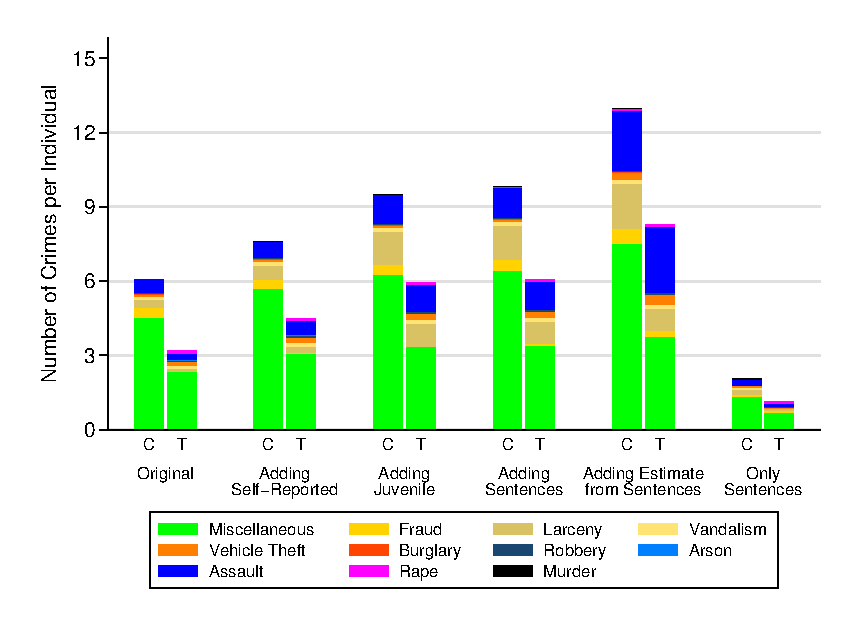
\includegraphics{AppOutput/Crime/counts_misc}}}
\floatfoot{
\footnotesize
\noindent Note: This chart shows the arrests per capita for the control (C) and treatment (T) groups. The first pair of bars shows the original arrests data from the administrative adult dataset. The next pair adds the self-reported crimes that did not match with the original arrests data. The next pair adds data from the administrative juvenile dataset that did not match with the previous datasets. The next pair adds one arrest for every sentence that did not match with the previous datasets and one arrest for every sentence that had arrest data missing. The next pair adds $n$ arrests instead of one for each sentence, where $n$ is calculated using the arrests-to-sentences ratio obtained from auxiliary datasets. The final pair of bars, for reference, is the total number of sentences from the administrative sentences dataset.
}
\end{figure}

\subsubsection{Construct Predictions}

\noindent The data available for the ABC subjects crimes committed up to age 34. However, we believe that the effect of the program on crime does not stop at that age. To predict the number of crimes that the study participants commit beyond age 34, we use data from the North Carolina Department of Public Safety (NCDPS). Because the crime data are obtained from the same state in which ABC was implemented, the prediction model is appropriate for the ABC sample. To the best of our knowledge, no study of the effects of an early childhood education program has ever used microdata to estimate a predictive model for future crimes. The estimations in \cite{Heckman_Moon_etal_2010_RateofReturn} are based on national age ratios (crimes of a certain category committed by older people over crimes of the same category committed by younger people at a specific time), rather than on microdata. However, age ratios only consider the same category of crime as an input to the estimation model and the results can reflect demographic transitions. \\

\noindent It would be ideal to use prediction models estimated from the same cohorts as the ABC participants. However, it is not possible to predict crimes committed until older ages because the ABC subjects are currently about 46 years old. To predict crimes at older ages, it is necessary to use earlier cohorts. The data are available from 1972 (44 years ago as of 2016), and thus they do not contain a complete criminal history for any cohort of individuals. 
%Given that, we have to choose specific cohorts for the estimations, such that they are old enough to cover the ages we need to predict, and young enough to have their entire crime life covered in the dataset, in the same way as the entire crime life of ABC individuals in covered in our data. In particular,
We assume that few crimes are committed after the age of 50. \\
%, and that crime life does not start until age 16.
 We separately estimate predictions from ages 35-40, 40-45, and 45-50. We have plentiful observations to estimate crimes in all the age ranges. %\footnote{As an example, to predict crimes at ages 45-50 we need individuals aged 50+. To have enough birth year cohorts, we consider individuals aged 50-59 in 2015. The oldest of these individuals were aged 16 in 1972, so we can reasonably expect them to having committed few crimes before that year. Finding observations for crime predictions at earlier ages is even easier.}
%Age 5 in 2015-->Age 12 in 1972.            Age 50 in 2015-->Age 16 in 1972.
%Age 55 in 2015-->Age 12 in 1972.            Age 59 in 2015-->Age 16 in 1972.
We calculate our predictions using a five-step procedure: \\
\begin{enumerate}
\item Find individuals that are at least 40 years old as of 2016 in the NCDPS dataset.
\item Regress the number of crimes of each type at ages 35--40 on those at ages 16--34.
\item Use the estimated prediction model for ABC individuals, attributing those crimes to age 40 for discounting purposes.
\item Repeat the three previous steps for ages 40--45 and 45--50. %50-55?
\item For individuals with no criminal histories before age 34, assume that they commit no crimes after 34.
\end{enumerate}

\noindent We perform the previous process separately for males and females. We use linear predictions, but replace negative predicted values of crime by zero. Table~\ref{tab:reg1f} through Table~\ref{tab:reg3m} show the estimated models. As expected, generally the most important prediction factor for a crime is the number of occurrences of the same crime type in a previous period. The coefficients in some cases are substantial, which implies that considering predicted crimes is an important part of an assessment of the crime benefits of the program. \\
%include more tables if ages 55 are covered, not just 50
\begin{sidewaystable}[H]
\caption{NCDPS Regressions of Ages 35--40 on Ages 16--35, Females} \label{tab:reg1f}
\begin{adjustbox}{max width=\textwidth}
\begin{threeparttable}
\begin{tabular}{lccccccccccc}
\hline\hline \noalign{\smallskip} & Miscellaneous & Fraud & Larceny & Vandalism & Auto Theft & Burglary & Robbery & Arson & Assault & Rape & Murder\\
\noalign{\smallskip}\hline \noalign{\smallskip}Miscellaneous & 0.103 & -0.029 & 0.009 & 0.001 & 0.001 & 0.001 & 0.000 & -0.000 & 0.002 & -0.000 & -0.001\\
 & \begin{footnotesize}(27.71)**\end{footnotesize} & \begin{footnotesize}(5.90)**\end{footnotesize} & \begin{footnotesize}(6.00)**\end{footnotesize} & \begin{footnotesize}(3.88)**\end{footnotesize} & \begin{footnotesize}(5.18)**\end{footnotesize} & \begin{footnotesize}(2.25)*\end{footnotesize} & \begin{footnotesize}(1.91)\end{footnotesize} & \begin{footnotesize}(0.62)\end{footnotesize} & \begin{footnotesize}(3.16)**\end{footnotesize} & \begin{footnotesize}(1.27)\end{footnotesize} & \begin{footnotesize}(2.85)**\end{footnotesize}\\
\noalign{\smallskip}Fraud & -0.047 & 0.104 & 0.003 & -0.000 & 0.000 & 0.000 & 0.000 & 0.000 & -0.001 & -0.000 & -0.000\\
 & \begin{footnotesize}(21.71)**\end{footnotesize} & \begin{footnotesize}(36.61)**\end{footnotesize} & \begin{footnotesize}(3.81)**\end{footnotesize} & \begin{footnotesize}(2.31)*\end{footnotesize} & \begin{footnotesize}(0.60)\end{footnotesize} & \begin{footnotesize}(2.02)*\end{footnotesize} & \begin{footnotesize}(0.02)\end{footnotesize} & \begin{footnotesize}(1.76)\end{footnotesize} & \begin{footnotesize}(1.48)\end{footnotesize} & \begin{footnotesize}(0.75)\end{footnotesize} & \begin{footnotesize}(1.72)\end{footnotesize}\\
\noalign{\smallskip}Larceny & 0.034 & 0.002 & 0.105 & 0.001 & 0.002 & 0.002 & 0.001 & 0.000 & 0.004 & 0.000 & -0.000\\
 & \begin{footnotesize}(8.16)**\end{footnotesize} & \begin{footnotesize}(0.33)\end{footnotesize} & \begin{footnotesize}(62.36)**\end{footnotesize} & \begin{footnotesize}(2.37)*\end{footnotesize} & \begin{footnotesize}(10.35)**\end{footnotesize} & \begin{footnotesize}(7.80)**\end{footnotesize} & \begin{footnotesize}(5.97)**\end{footnotesize} & \begin{footnotesize}(2.99)**\end{footnotesize} & \begin{footnotesize}(5.65)**\end{footnotesize} & \begin{footnotesize}(1.30)\end{footnotesize} & \begin{footnotesize}(1.67)\end{footnotesize}\\
\noalign{\smallskip}Vandal & 0.000 & -0.036 & -0.024 & 0.012 & 0.004 & 0.007 & 0.005 & 0.003 & 0.043 & 0.000 & -0.000\\
 & \begin{footnotesize}(0.01)\end{footnotesize} & \begin{footnotesize}(1.10)\end{footnotesize} & \begin{footnotesize}(2.43)*\end{footnotesize} & \begin{footnotesize}(6.40)**\end{footnotesize} & \begin{footnotesize}(2.86)**\end{footnotesize} & \begin{footnotesize}(3.87)**\end{footnotesize} & \begin{footnotesize}(3.34)**\end{footnotesize} & \begin{footnotesize}(3.40)**\end{footnotesize} & \begin{footnotesize}(9.27)**\end{footnotesize} & \begin{footnotesize}(0.79)\end{footnotesize} & \begin{footnotesize}(0.23)\end{footnotesize}\\
\noalign{\smallskip}Auto Theft & 0.059 & -0.026 & 0.055 & 0.004 & 0.012 & 0.007 & 0.005 & -0.002 & -0.014 & -0.000 & 0.002\\
 & \begin{footnotesize}(1.55)\end{footnotesize} & \begin{footnotesize}(0.52)\end{footnotesize} & \begin{footnotesize}(3.57)**\end{footnotesize} & \begin{footnotesize}(1.28)\end{footnotesize} & \begin{footnotesize}(5.94)**\end{footnotesize} & \begin{footnotesize}(2.48)*\end{footnotesize} & \begin{footnotesize}(2.52)*\end{footnotesize} & \begin{footnotesize}(1.30)\end{footnotesize} & \begin{footnotesize}(2.02)*\end{footnotesize} & \begin{footnotesize}(0.23)\end{footnotesize} & \begin{footnotesize}(1.02)\end{footnotesize}\\
\noalign{\smallskip}Burglary & 0.049 & -0.031 & 0.011 & 0.002 & 0.006 & 0.044 & 0.000 & -0.001 & -0.003 & -0.000 & -0.001\\
 & \begin{footnotesize}(1.77)\end{footnotesize} & \begin{footnotesize}(0.86)\end{footnotesize} & \begin{footnotesize}(1.01)\end{footnotesize} & \begin{footnotesize}(0.95)\end{footnotesize} & \begin{footnotesize}(3.86)**\end{footnotesize} & \begin{footnotesize}(22.56)**\end{footnotesize} & \begin{footnotesize}(0.20)\end{footnotesize} & \begin{footnotesize}(1.26)\end{footnotesize} & \begin{footnotesize}(0.55)\end{footnotesize} & \begin{footnotesize}(0.25)\end{footnotesize} & \begin{footnotesize}(0.34)\end{footnotesize}\\
\noalign{\smallskip}Robbery & 0.030 & 0.054 & 0.040 & 0.002 & 0.005 & -0.001 & 0.028 & 0.002 & -0.000 & -0.000 & 0.002\\
 & \begin{footnotesize}(1.05)\end{footnotesize} & \begin{footnotesize}(1.46)\end{footnotesize} & \begin{footnotesize}(3.51)**\end{footnotesize} & \begin{footnotesize}(1.03)\end{footnotesize} & \begin{footnotesize}(3.43)**\end{footnotesize} & \begin{footnotesize}(0.28)\end{footnotesize} & \begin{footnotesize}(17.69)**\end{footnotesize} & \begin{footnotesize}(2.22)*\end{footnotesize} & \begin{footnotesize}(0.07)\end{footnotesize} & \begin{footnotesize}(0.29)\end{footnotesize} & \begin{footnotesize}(1.50)\end{footnotesize}\\
\noalign{\smallskip}Arson & 0.070 & -0.087 & -0.035 & 0.008 & 0.011 & 0.006 & 0.025 & 0.010 & 0.017 & -0.000 & 0.005\\
 & \begin{footnotesize}(1.29)\end{footnotesize} & \begin{footnotesize}(1.22)\end{footnotesize} & \begin{footnotesize}(1.61)\end{footnotesize} & \begin{footnotesize}(1.98)*\end{footnotesize} & \begin{footnotesize}(3.98)**\end{footnotesize} & \begin{footnotesize}(1.62)\end{footnotesize} & \begin{footnotesize}(8.19)**\end{footnotesize} & \begin{footnotesize}(4.95)**\end{footnotesize} & \begin{footnotesize}(1.67)\end{footnotesize} & \begin{footnotesize}(0.19)\end{footnotesize} & \begin{footnotesize}(1.60)\end{footnotesize}\\
\noalign{\smallskip}Assault & 0.064 & -0.060 & 0.007 & 0.007 & 0.001 & 0.002 & -0.000 & 0.002 & 0.048 & -0.000 & 0.000\\
 & \begin{footnotesize}(5.74)**\end{footnotesize} & \begin{footnotesize}(4.11)**\end{footnotesize} & \begin{footnotesize}(1.63)\end{footnotesize} & \begin{footnotesize}(7.82)**\end{footnotesize} & \begin{footnotesize}(1.83)\end{footnotesize} & \begin{footnotesize}(1.93)\end{footnotesize} & \begin{footnotesize}(0.14)\end{footnotesize} & \begin{footnotesize}(4.52)**\end{footnotesize} & \begin{footnotesize}(22.78)**\end{footnotesize} & \begin{footnotesize}(0.36)\end{footnotesize} & \begin{footnotesize}(0.34)\end{footnotesize}\\
\noalign{\smallskip}Rape & -0.015 & -0.131 & -0.003 & -0.003 & -0.003 & -0.004 & -0.006 & -0.001 & 0.001 & -0.000 & -0.002\\
 & \begin{footnotesize}(0.15)\end{footnotesize} & \begin{footnotesize}(0.98)\end{footnotesize} & \begin{footnotesize}(0.08)\end{footnotesize} & \begin{footnotesize}(0.42)\end{footnotesize} & \begin{footnotesize}(0.49)\end{footnotesize} & \begin{footnotesize}(0.55)\end{footnotesize} & \begin{footnotesize}(0.99)\end{footnotesize} & \begin{footnotesize}(0.24)\end{footnotesize} & \begin{footnotesize}(0.08)\end{footnotesize} & \begin{footnotesize}(0.06)\end{footnotesize} & \begin{footnotesize}(0.33)\end{footnotesize}\\
\noalign{\smallskip}Murder & 0.006 & -0.166 & -0.008 & 0.003 & -0.002 & -0.002 & -0.002 & 0.003 & 0.001 & -0.000 & -0.001\\
 & \begin{footnotesize}(0.16)\end{footnotesize} & \begin{footnotesize}(3.44)**\end{footnotesize} & \begin{footnotesize}(0.54)\end{footnotesize} & \begin{footnotesize}(1.19)\end{footnotesize} & \begin{footnotesize}(0.94)\end{footnotesize} & \begin{footnotesize}(0.75)\end{footnotesize} & \begin{footnotesize}(1.22)\end{footnotesize} & \begin{footnotesize}(2.24)*\end{footnotesize} & \begin{footnotesize}(0.12)\end{footnotesize} & \begin{footnotesize}(0.34)\end{footnotesize} & \begin{footnotesize}(0.37)\end{footnotesize}\\
\noalign{\smallskip}constant & 0.069 & 0.267 & 0.041 & 0.004 & 0.001 & 0.001 & 0.001 & 0.001 & 0.023 & 0.000 & 0.004\\
 & \begin{footnotesize}(13.39)**\end{footnotesize} & \begin{footnotesize}(39.01)**\end{footnotesize} & \begin{footnotesize}(19.54)**\end{footnotesize} & \begin{footnotesize}(10.27)**\end{footnotesize} & \begin{footnotesize}(2.76)**\end{footnotesize} & \begin{footnotesize}(3.17)**\end{footnotesize} & \begin{footnotesize}(4.80)**\end{footnotesize} & \begin{footnotesize}(3.52)**\end{footnotesize} & \begin{footnotesize}(23.81)**\end{footnotesize} & \begin{footnotesize}(3.38)**\end{footnotesize} & \begin{footnotesize}(12.90)**\end{footnotesize}\\
\noalign{\smallskip}$R^2$ & 0.02 & 0.02 & 0.07 & 0.00 & 0.01 & 0.01 & 0.01 & 0.00 & 0.01 & 0.00 & 0.00\\
$N$ & 63,515 & 63,515 & 63,515 & 63,515 & 63,515 & 63,515 & 63,515 & 63,515 & 63,515 & 63,515 & 63,515\\
\noalign{\smallskip}\hline\hline\end{tabular}

\begin{tablenotes}
\item Note: This table shows how the crimes at ages 35--40 (in the columns) are predicted by crimes at ages 16--35 (in the rows). The estimations are predicted using the North Carolina Department of Public Safety dataset, which contains information on all individuals that have ever been sentenced in North Carolina. We use linear regressions in all cases. The sample for this model is limited to individuals who are at least 40 years old. *~$p<0.05$; **~$p<0.01$.
\end{tablenotes}
\end{threeparttable}
\end{adjustbox}
\end{sidewaystable}


\begin{sidewaystable}[H]
\caption{NCDPS Regressions of Ages 35--40 on Ages 16--35, Males} \label{tab:reg1m}
\begin{adjustbox}{max width=\textwidth}
\begin{threeparttable}
\begin{tabular}{lccccccccccc}
\hline\hline \noalign{\smallskip} & Miscellaneous & Fraud & Larceny & Vandalism & Auto Theft & Burglary & Robbery & Arson & Assault & Rape & Murder\\
\noalign{\smallskip}\hline \noalign{\smallskip}Miscellaneous & 0.095 & -0.002 & 0.004 & 0.000 & 0.001 & 0.001 & 0.000 & -0.000 & 0.005 & -0.001 & -0.001\\
 & \begin{footnotesize}(73.29)**\end{footnotesize} & \begin{footnotesize}(2.13)*\end{footnotesize} & \begin{footnotesize}(8.97)**\end{footnotesize} & \begin{footnotesize}(2.71)**\end{footnotesize} & \begin{footnotesize}(6.47)**\end{footnotesize} & \begin{footnotesize}(5.87)**\end{footnotesize} & \begin{footnotesize}(1.50)\end{footnotesize} & \begin{footnotesize}(0.12)\end{footnotesize} & \begin{footnotesize}(14.73)**\end{footnotesize} & \begin{footnotesize}(3.28)**\end{footnotesize} & \begin{footnotesize}(5.83)**\end{footnotesize}\\
\noalign{\smallskip}Fraud & -0.025 & 0.107 & 0.007 & 0.000 & 0.001 & 0.002 & 0.001 & -0.000 & -0.000 & -0.000 & -0.000\\
 & \begin{footnotesize}(13.76)**\end{footnotesize} & \begin{footnotesize}(67.23)**\end{footnotesize} & \begin{footnotesize}(11.68)**\end{footnotesize} & \begin{footnotesize}(0.47)\end{footnotesize} & \begin{footnotesize}(3.44)**\end{footnotesize} & \begin{footnotesize}(5.27)**\end{footnotesize} & \begin{footnotesize}(2.53)*\end{footnotesize} & \begin{footnotesize}(0.61)\end{footnotesize} & \begin{footnotesize}(0.34)\end{footnotesize} & \begin{footnotesize}(0.35)\end{footnotesize} & \begin{footnotesize}(1.96)*\end{footnotesize}\\
\noalign{\smallskip}Larceny & 0.041 & 0.012 & 0.092 & 0.001 & 0.005 & 0.010 & 0.004 & 0.000 & 0.009 & -0.000 & -0.000\\
 & \begin{footnotesize}(14.34)**\end{footnotesize} & \begin{footnotesize}(4.83)**\end{footnotesize} & \begin{footnotesize}(97.06)**\end{footnotesize} & \begin{footnotesize}(5.13)**\end{footnotesize} & \begin{footnotesize}(14.85)**\end{footnotesize} & \begin{footnotesize}(19.72)**\end{footnotesize} & \begin{footnotesize}(12.30)**\end{footnotesize} & \begin{footnotesize}(1.79)\end{footnotesize} & \begin{footnotesize}(11.37)**\end{footnotesize} & \begin{footnotesize}(0.46)\end{footnotesize} & \begin{footnotesize}(0.59)\end{footnotesize}\\
\noalign{\smallskip}Vandal & 0.041 & -0.017 & -0.007 & 0.019 & 0.002 & 0.002 & 0.002 & 0.002 & 0.029 & 0.001 & 0.000\\
 & \begin{footnotesize}(4.51)**\end{footnotesize} & \begin{footnotesize}(2.13)*\end{footnotesize} & \begin{footnotesize}(2.22)*\end{footnotesize} & \begin{footnotesize}(23.49)**\end{footnotesize} & \begin{footnotesize}(1.96)\end{footnotesize} & \begin{footnotesize}(1.06)\end{footnotesize} & \begin{footnotesize}(1.76)\end{footnotesize} & \begin{footnotesize}(5.41)**\end{footnotesize} & \begin{footnotesize}(11.26)**\end{footnotesize} & \begin{footnotesize}(1.06)\end{footnotesize} & \begin{footnotesize}(0.62)\end{footnotesize}\\
\noalign{\smallskip}Auto Theft & 0.015 & 0.014 & 0.005 & 0.002 & 0.043 & 0.013 & 0.000 & 0.000 & 0.008 & 0.001 & 0.001\\
 & \begin{footnotesize}(1.58)\end{footnotesize} & \begin{footnotesize}(1.70)\end{footnotesize} & \begin{footnotesize}(1.48)\end{footnotesize} & \begin{footnotesize}(1.86)\end{footnotesize} & \begin{footnotesize}(39.51)**\end{footnotesize} & \begin{footnotesize}(7.87)**\end{footnotesize} & \begin{footnotesize}(0.14)\end{footnotesize} & \begin{footnotesize}(0.13)\end{footnotesize} & \begin{footnotesize}(3.12)**\end{footnotesize} & \begin{footnotesize}(1.28)\end{footnotesize} & \begin{footnotesize}(1.18)\end{footnotesize}\\
\noalign{\smallskip}Burglary & 0.005 & 0.011 & 0.010 & 0.002 & 0.004 & 0.040 & 0.003 & -0.000 & 0.003 & 0.001 & -0.000\\
 & \begin{footnotesize}(1.26)\end{footnotesize} & \begin{footnotesize}(3.06)**\end{footnotesize} & \begin{footnotesize}(6.86)**\end{footnotesize} & \begin{footnotesize}(4.33)**\end{footnotesize} & \begin{footnotesize}(9.17)**\end{footnotesize} & \begin{footnotesize}(52.89)**\end{footnotesize} & \begin{footnotesize}(6.55)**\end{footnotesize} & \begin{footnotesize}(0.30)\end{footnotesize} & \begin{footnotesize}(2.34)*\end{footnotesize} & \begin{footnotesize}(2.37)*\end{footnotesize} & \begin{footnotesize}(0.73)\end{footnotesize}\\
\noalign{\smallskip}Robbery & -0.032 & 0.000 & 0.011 & 0.000 & 0.003 & 0.006 & 0.019 & -0.000 & -0.000 & 0.000 & 0.001\\
 & \begin{footnotesize}(5.06)**\end{footnotesize} & \begin{footnotesize}(0.01)\end{footnotesize} & \begin{footnotesize}(5.42)**\end{footnotesize} & \begin{footnotesize}(0.67)\end{footnotesize} & \begin{footnotesize}(4.61)**\end{footnotesize} & \begin{footnotesize}(5.67)**\end{footnotesize} & \begin{footnotesize}(26.50)**\end{footnotesize} & \begin{footnotesize}(1.00)\end{footnotesize} & \begin{footnotesize}(0.21)\end{footnotesize} & \begin{footnotesize}(0.00)\end{footnotesize} & \begin{footnotesize}(1.68)\end{footnotesize}\\
\noalign{\smallskip}Arson & 0.008 & -0.023 & -0.010 & 0.012 & -0.004 & 0.008 & 0.004 & 0.007 & 0.031 & -0.001 & 0.001\\
 & \begin{footnotesize}(0.26)\end{footnotesize} & \begin{footnotesize}(0.82)\end{footnotesize} & \begin{footnotesize}(0.95)\end{footnotesize} & \begin{footnotesize}(4.40)**\end{footnotesize} & \begin{footnotesize}(0.98)\end{footnotesize} & \begin{footnotesize}(1.44)\end{footnotesize} & \begin{footnotesize}(1.22)\end{footnotesize} & \begin{footnotesize}(6.73)**\end{footnotesize} & \begin{footnotesize}(3.49)**\end{footnotesize} & \begin{footnotesize}(0.21)\end{footnotesize} & \begin{footnotesize}(0.39)\end{footnotesize}\\
\noalign{\smallskip}Assault & 0.041 & -0.010 & -0.000 & 0.005 & -0.001 & 0.000 & 0.002 & 0.000 & 0.051 & 0.001 & 0.001\\
 & \begin{footnotesize}(11.14)**\end{footnotesize} & \begin{footnotesize}(3.18)**\end{footnotesize} & \begin{footnotesize}(0.09)\end{footnotesize} & \begin{footnotesize}(15.94)**\end{footnotesize} & \begin{footnotesize}(1.60)\end{footnotesize} & \begin{footnotesize}(0.12)\end{footnotesize} & \begin{footnotesize}(4.47)**\end{footnotesize} & \begin{footnotesize}(2.56)*\end{footnotesize} & \begin{footnotesize}(49.57)**\end{footnotesize} & \begin{footnotesize}(3.43)**\end{footnotesize} & \begin{footnotesize}(3.29)**\end{footnotesize}\\
\noalign{\smallskip}Rape & -0.003 & -0.016 & -0.010 & -0.002 & -0.002 & -0.006 & -0.002 & -0.000 & -0.004 & 0.011 & -0.001\\
 & \begin{footnotesize}(0.33)\end{footnotesize} & \begin{footnotesize}(1.77)\end{footnotesize} & \begin{footnotesize}(2.86)**\end{footnotesize} & \begin{footnotesize}(2.32)*\end{footnotesize} & \begin{footnotesize}(1.72)\end{footnotesize} & \begin{footnotesize}(3.42)**\end{footnotesize} & \begin{footnotesize}(1.66)\end{footnotesize} & \begin{footnotesize}(0.54)\end{footnotesize} & \begin{footnotesize}(1.21)\end{footnotesize} & \begin{footnotesize}(8.61)**\end{footnotesize} & \begin{footnotesize}(1.69)\end{footnotesize}\\
\noalign{\smallskip}Murder & -0.086 & -0.053 & -0.025 & -0.002 & -0.004 & -0.011 & -0.001 & -0.001 & -0.007 & -0.003 & 0.003\\
 & \begin{footnotesize}(6.33)**\end{footnotesize} & \begin{footnotesize}(4.45)**\end{footnotesize} & \begin{footnotesize}(5.51)**\end{footnotesize} & \begin{footnotesize}(1.71)\end{footnotesize} & \begin{footnotesize}(2.54)*\end{footnotesize} & \begin{footnotesize}(4.31)**\end{footnotesize} & \begin{footnotesize}(0.87)\end{footnotesize} & \begin{footnotesize}(1.53)\end{footnotesize} & \begin{footnotesize}(1.79)\end{footnotesize} & \begin{footnotesize}(1.56)\end{footnotesize} & \begin{footnotesize}(3.35)**\end{footnotesize}\\
\noalign{\smallskip}constant & 0.213 & 0.124 & 0.031 & 0.005 & 0.004 & 0.011 & 0.006 & 0.001 & 0.048 & 0.009 & 0.006\\
 & \begin{footnotesize}(69.25)**\end{footnotesize} & \begin{footnotesize}(45.55)**\end{footnotesize} & \begin{footnotesize}(29.74)**\end{footnotesize} & \begin{footnotesize}(18.57)**\end{footnotesize} & \begin{footnotesize}(10.95)**\end{footnotesize} & \begin{footnotesize}(19.97)**\end{footnotesize} & \begin{footnotesize}(17.78)**\end{footnotesize} & \begin{footnotesize}(9.22)**\end{footnotesize} & \begin{footnotesize}(55.54)**\end{footnotesize} & \begin{footnotesize}(24.70)**\end{footnotesize} & \begin{footnotesize}(27.76)**\end{footnotesize}\\
\noalign{\smallskip}$R^2$ & 0.03 & 0.02 & 0.05 & 0.01 & 0.01 & 0.02 & 0.01 & 0.00 & 0.02 & 0.00 & 0.00\\
$N$ & 230,706 & 230,706 & 230,706 & 230,706 & 230,706 & 230,706 & 230,706 & 230,706 & 230,706 & 230,706 & 230,706\\
\noalign{\smallskip}\hline\hline\end{tabular}

\begin{tablenotes}
\item Note: This table shows how the crimes at ages 35--40 (in the columns) are predicted by crimes at ages 16--35 (in the rows). The estimations are predicted using the North Carolina Department of Public Safety dataset, which contains information on all individuals that have ever been sentenced in North Carolina. We use linear regressions in all cases. The sample for this model is limited to individuals who are at least 40 years old. *~$p<0.05$; **~$p<0.01$.
\end{tablenotes}
\end{threeparttable}
\end{adjustbox}
\end{sidewaystable}

\begin{sidewaystable}[H]
\caption{NCDPS Regressions of Ages 40--45 on Ages 16--35, Females} \label{tab:reg2f}
\begin{adjustbox}{max width=\textwidth}
\begin{threeparttable}
\begin{tabular}{lccccccccccc}
\toprule \noalign{\smallskip} & Miscellaneous & Fraud & Larceny & Vandalism & Auto Theft & Burglary & Robbery & Arson & Assault & Rape & Murder\\
\noalign{\smallskip}\midrule \noalign{\smallskip}Miscellaneous & 0.020 & -0.006 & -0.001 & 0.000 & 0.000 & 0.000 & -0.000 & 0.000 & 0.001 & 0.000 & -0.001\\
 & \begin{footnotesize}(4.33)**\end{footnotesize} & \begin{footnotesize}(5.18)**\end{footnotesize} & \begin{footnotesize}(0.85)\end{footnotesize} & \begin{footnotesize}(0.78)\end{footnotesize} & \begin{footnotesize}(0.46)\end{footnotesize} & \begin{footnotesize}(1.29)\end{footnotesize} & \begin{footnotesize}(0.11)\end{footnotesize} & \begin{footnotesize}(0.84)\end{footnotesize} & \begin{footnotesize}(0.64)\end{footnotesize} & \begin{footnotesize}(3.66)**\end{footnotesize} & \begin{footnotesize}(2.65)**\end{footnotesize}\\
\noalign{\smallskip}Fraud & 0.046 & 0.003 & 0.002 & 0.000 & 0.001 & -0.000 & 0.000 & -0.000 & -0.000 & 0.000 & -0.000\\
 & \begin{footnotesize}(19.30)**\end{footnotesize} & \begin{footnotesize}(4.41)**\end{footnotesize} & \begin{footnotesize}(2.86)**\end{footnotesize} & \begin{footnotesize}(1.50)\end{footnotesize} & \begin{footnotesize}(4.86)**\end{footnotesize} & \begin{footnotesize}(0.56)\end{footnotesize} & \begin{footnotesize}(1.62)\end{footnotesize} & \begin{footnotesize}(0.62)\end{footnotesize} & \begin{footnotesize}(1.13)\end{footnotesize} & \begin{footnotesize}(2.50)*\end{footnotesize} & \begin{footnotesize}(0.44)\end{footnotesize}\\
\noalign{\smallskip}Larceny & 0.025 & -0.002 & 0.070 & 0.000 & 0.001 & 0.002 & 0.000 & -0.000 & 0.004 & -0.000 & -0.000\\
 & \begin{footnotesize}(5.12)**\end{footnotesize} & \begin{footnotesize}(1.54)\end{footnotesize} & \begin{footnotesize}(41.35)**\end{footnotesize} & \begin{footnotesize}(0.06)\end{footnotesize} & \begin{footnotesize}(3.61)**\end{footnotesize} & \begin{footnotesize}(6.68)**\end{footnotesize} & \begin{footnotesize}(0.75)\end{footnotesize} & \begin{footnotesize}(1.27)\end{footnotesize} & \begin{footnotesize}(5.02)**\end{footnotesize} & \begin{footnotesize}(0.45)\end{footnotesize} & \begin{footnotesize}(0.45)\end{footnotesize}\\
\noalign{\smallskip}Vandal & -0.016 & -0.009 & -0.018 & 0.002 & -0.001 & 0.005 & 0.001 & 0.003 & 0.019 & -0.000 & -0.001\\
 & \begin{footnotesize}(0.52)\end{footnotesize} & \begin{footnotesize}(1.22)\end{footnotesize} & \begin{footnotesize}(1.71)\end{footnotesize} & \begin{footnotesize}(1.02)\end{footnotesize} & \begin{footnotesize}(0.58)\end{footnotesize} & \begin{footnotesize}(2.66)**\end{footnotesize} & \begin{footnotesize}(0.38)\end{footnotesize} & \begin{footnotesize}(3.06)**\end{footnotesize} & \begin{footnotesize}(3.54)**\end{footnotesize} & \begin{footnotesize}(0.71)\end{footnotesize} & \begin{footnotesize}(0.49)\end{footnotesize}\\
\noalign{\smallskip}Auto Theft & 0.012 & -0.011 & 0.010 & 0.004 & 0.012 & 0.013 & -0.001 & -0.001 & -0.017 & 0.007 & 0.001\\
 & \begin{footnotesize}(0.25)\end{footnotesize} & \begin{footnotesize}(0.87)\end{footnotesize} & \begin{footnotesize}(0.56)\end{footnotesize} & \begin{footnotesize}(0.95)\end{footnotesize} & \begin{footnotesize}(4.90)**\end{footnotesize} & \begin{footnotesize}(4.70)**\end{footnotesize} & \begin{footnotesize}(0.36)\end{footnotesize} & \begin{footnotesize}(0.49)\end{footnotesize} & \begin{footnotesize}(1.98)*\end{footnotesize} & \begin{footnotesize}(11.24)**\end{footnotesize} & \begin{footnotesize}(0.41)\end{footnotesize}\\
\noalign{\smallskip}Burglary & -0.034 & 0.019 & 0.007 & -0.003 & 0.005 & 0.007 & 0.004 & 0.000 & -0.004 & 0.001 & -0.001\\
 & \begin{footnotesize}(1.05)\end{footnotesize} & \begin{footnotesize}(2.33)*\end{footnotesize} & \begin{footnotesize}(0.64)\end{footnotesize} & \begin{footnotesize}(1.05)\end{footnotesize} & \begin{footnotesize}(3.12)**\end{footnotesize} & \begin{footnotesize}(3.66)**\end{footnotesize} & \begin{footnotesize}(2.09)*\end{footnotesize} & \begin{footnotesize}(0.22)\end{footnotesize} & \begin{footnotesize}(0.67)\end{footnotesize} & \begin{footnotesize}(2.93)**\end{footnotesize} & \begin{footnotesize}(0.55)\end{footnotesize}\\
\noalign{\smallskip}Robbery & 0.027 & 0.004 & 0.021 & 0.004 & 0.002 & 0.007 & 0.015 & -0.001 & 0.018 & -0.000 & -0.001\\
 & \begin{footnotesize}(0.81)\end{footnotesize} & \begin{footnotesize}(0.47)\end{footnotesize} & \begin{footnotesize}(1.81)\end{footnotesize} & \begin{footnotesize}(1.52)\end{footnotesize} & \begin{footnotesize}(1.21)\end{footnotesize} & \begin{footnotesize}(3.98)**\end{footnotesize} & \begin{footnotesize}(6.93)**\end{footnotesize} & \begin{footnotesize}(0.58)\end{footnotesize} & \begin{footnotesize}(3.19)**\end{footnotesize} & \begin{footnotesize}(0.67)\end{footnotesize} & \begin{footnotesize}(0.82)\end{footnotesize}\\
\noalign{\smallskip}Arson & -0.042 & -0.016 & -0.025 & 0.013 & -0.001 & -0.002 & 0.001 & -0.001 & 0.001 & -0.000 & -0.002\\
 & \begin{footnotesize}(0.65)\end{footnotesize} & \begin{footnotesize}(0.97)\end{footnotesize} & \begin{footnotesize}(1.09)\end{footnotesize} & \begin{footnotesize}(2.63)**\end{footnotesize} & \begin{footnotesize}(0.46)\end{footnotesize} & \begin{footnotesize}(0.57)\end{footnotesize} & \begin{footnotesize}(0.31)\end{footnotesize} & \begin{footnotesize}(0.44)\end{footnotesize} & \begin{footnotesize}(0.12)\end{footnotesize} & \begin{footnotesize}(0.06)\end{footnotesize} & \begin{footnotesize}(0.56)\end{footnotesize}\\
\noalign{\smallskip}Assault & -0.014 & -0.008 & -0.007 & 0.002 & -0.000 & -0.001 & 0.002 & 0.001 & 0.028 & -0.000 & -0.000\\
 & \begin{footnotesize}(1.00)\end{footnotesize} & \begin{footnotesize}(2.44)*\end{footnotesize} & \begin{footnotesize}(1.41)\end{footnotesize} & \begin{footnotesize}(1.84)\end{footnotesize} & \begin{footnotesize}(0.20)\end{footnotesize} & \begin{footnotesize}(1.21)\end{footnotesize} & \begin{footnotesize}(2.10)*\end{footnotesize} & \begin{footnotesize}(2.34)*\end{footnotesize} & \begin{footnotesize}(11.83)**\end{footnotesize} & \begin{footnotesize}(1.23)\end{footnotesize} & \begin{footnotesize}(0.41)\end{footnotesize}\\
\noalign{\smallskip}Rape & 0.169 & -0.014 & -0.029 & -0.003 & -0.002 & -0.003 & -0.004 & -0.000 & -0.016 & -0.000 & 0.011\\
 & \begin{footnotesize}(1.36)\end{footnotesize} & \begin{footnotesize}(0.45)\end{footnotesize} & \begin{footnotesize}(0.67)\end{footnotesize} & \begin{footnotesize}(0.36)\end{footnotesize} & \begin{footnotesize}(0.29)\end{footnotesize} & \begin{footnotesize}(0.46)\end{footnotesize} & \begin{footnotesize}(0.57)\end{footnotesize} & \begin{footnotesize}(0.07)\end{footnotesize} & \begin{footnotesize}(0.75)\end{footnotesize} & \begin{footnotesize}(0.05)\end{footnotesize} & \begin{footnotesize}(1.91)\end{footnotesize}\\
\noalign{\smallskip}Murder & -0.169 & -0.022 & -0.027 & -0.004 & -0.002 & -0.002 & 0.001 & -0.001 & 0.010 & -0.000 & -0.001\\
 & \begin{footnotesize}(4.25)**\end{footnotesize} & \begin{footnotesize}(2.18)*\end{footnotesize} & \begin{footnotesize}(1.93)\end{footnotesize} & \begin{footnotesize}(1.38)\end{footnotesize} & \begin{footnotesize}(0.84)\end{footnotesize} & \begin{footnotesize}(0.91)\end{footnotesize} & \begin{footnotesize}(0.55)\end{footnotesize} & \begin{footnotesize}(0.64)\end{footnotesize} & \begin{footnotesize}(1.46)\end{footnotesize} & \begin{footnotesize}(0.06)\end{footnotesize} & \begin{footnotesize}(0.50)\end{footnotesize}\\
\noalign{\smallskip}constant & 0.304 & 0.029 & 0.046 & 0.005 & 0.002 & 0.002 & 0.002 & 0.001 & 0.022 & -0.000 & 0.003\\
 & \begin{footnotesize}(53.09)**\end{footnotesize} & \begin{footnotesize}(20.43)**\end{footnotesize} & \begin{footnotesize}(22.75)**\end{footnotesize} & \begin{footnotesize}(10.59)**\end{footnotesize} & \begin{footnotesize}(5.51)**\end{footnotesize} & \begin{footnotesize}(4.90)**\end{footnotesize} & \begin{footnotesize}(4.93)**\end{footnotesize} & \begin{footnotesize}(4.52)**\end{footnotesize} & \begin{footnotesize}(22.64)**\end{footnotesize} & \begin{footnotesize}(0.48)\end{footnotesize} & \begin{footnotesize}(11.16)**\end{footnotesize}\\
\noalign{\smallskip}$R^2$ & 0.01 & 0.00 & 0.04 & 0.00 & 0.00 & 0.00 & 0.00 & 0.00 & 0.00 & 0.00 & 0.00\\
$N$ & 49,738 & 49,738 & 49,738 & 49,738 & 49,738 & 49,738 & 49,738 & 49,738 & 49,738 & 49,738 & 49,738\\
\noalign{\smallskip}\bottomrule\end{tabular}

\begin{tablenotes}
\item Note: This table shows how the crimes at ages 40--45 (in the columns) are predicted by crimes at ages 16--35 (in the rows). The estimations are predicted using the North Carolina Department of Public Safety dataset, which contains information on all individuals that have ever been sentenced in North Carolina. We use linear regressions in all cases. The sample for this model is limited to individuals who are at least 45 years old. *~$p<0.05$; **~$p<0.01$.
\end{tablenotes}
\end{threeparttable}
\end{adjustbox}
\end{sidewaystable}


\begin{sidewaystable}[H]
\caption{NCDPS Regressions of Ages 40--45 on Ages 16--35, Males} \label{tab:reg2m}
\begin{adjustbox}{max width=\textwidth}
\begin{threeparttable}
\begin{tabular}{lccccccccccc}
\hline\hline \noalign{\smallskip} & Miscellaneous & Fraud & Larceny & Vandalism & Auto Theft & Burglary & Robbery & Arson & Assault & Rape & Murder\\
\noalign{\smallskip}\hline \noalign{\smallskip}Miscellaneous & 0.065 & -0.002 & 0.003 & 0.001 & 0.001 & 0.001 & -0.000 & 0.000 & 0.003 & -0.000 & -0.001\\
 & \begin{footnotesize}(40.59)**\end{footnotesize} & \begin{footnotesize}(4.98)**\end{footnotesize} & \begin{footnotesize}(6.29)**\end{footnotesize} & \begin{footnotesize}(4.35)**\end{footnotesize} & \begin{footnotesize}(4.68)**\end{footnotesize} & \begin{footnotesize}(3.18)**\end{footnotesize} & \begin{footnotesize}(2.61)**\end{footnotesize} & \begin{footnotesize}(0.25)\end{footnotesize} & \begin{footnotesize}(7.80)**\end{footnotesize} & \begin{footnotesize}(2.60)**\end{footnotesize} & \begin{footnotesize}(6.70)**\end{footnotesize}\\
\noalign{\smallskip}Fraud & 0.032 & 0.009 & 0.004 & -0.000 & 0.001 & 0.002 & 0.000 & -0.000 & 0.000 & -0.000 & -0.000\\
 & \begin{footnotesize}(16.63)**\end{footnotesize} & \begin{footnotesize}(18.85)**\end{footnotesize} & \begin{footnotesize}(6.51)**\end{footnotesize} & \begin{footnotesize}(0.72)\end{footnotesize} & \begin{footnotesize}(5.79)**\end{footnotesize} & \begin{footnotesize}(5.19)**\end{footnotesize} & \begin{footnotesize}(2.29)*\end{footnotesize} & \begin{footnotesize}(0.83)\end{footnotesize} & \begin{footnotesize}(0.84)\end{footnotesize} & \begin{footnotesize}(1.28)\end{footnotesize} & \begin{footnotesize}(0.78)\end{footnotesize}\\
\noalign{\smallskip}Larceny & 0.029 & 0.001 & 0.055 & 0.002 & 0.003 & 0.005 & 0.002 & -0.000 & 0.004 & -0.000 & 0.000\\
 & \begin{footnotesize}(9.25)**\end{footnotesize} & \begin{footnotesize}(1.16)\end{footnotesize} & \begin{footnotesize}(54.05)**\end{footnotesize} & \begin{footnotesize}(6.64)**\end{footnotesize} & \begin{footnotesize}(11.18)**\end{footnotesize} & \begin{footnotesize}(9.45)**\end{footnotesize} & \begin{footnotesize}(8.46)**\end{footnotesize} & \begin{footnotesize}(2.55)*\end{footnotesize} & \begin{footnotesize}(4.35)**\end{footnotesize} & \begin{footnotesize}(0.64)\end{footnotesize} & \begin{footnotesize}(0.70)\end{footnotesize}\\
\noalign{\smallskip}Vandal & 0.003 & -0.001 & -0.009 & 0.007 & -0.000 & 0.002 & 0.001 & 0.000 & 0.024 & 0.001 & -0.000\\
 & \begin{footnotesize}(0.26)\end{footnotesize} & \begin{footnotesize}(0.46)\end{footnotesize} & \begin{footnotesize}(2.68)**\end{footnotesize} & \begin{footnotesize}(8.19)**\end{footnotesize} & \begin{footnotesize}(0.04)\end{footnotesize} & \begin{footnotesize}(1.05)\end{footnotesize} & \begin{footnotesize}(1.02)\end{footnotesize} & \begin{footnotesize}(1.29)\end{footnotesize} & \begin{footnotesize}(8.44)**\end{footnotesize} & \begin{footnotesize}(0.66)\end{footnotesize} & \begin{footnotesize}(0.37)\end{footnotesize}\\
\noalign{\smallskip}Auto Theft & 0.053 & 0.002 & 0.007 & 0.001 & 0.016 & 0.017 & 0.002 & 0.001 & 0.010 & 0.001 & 0.000\\
 & \begin{footnotesize}(4.40)**\end{footnotesize} & \begin{footnotesize}(0.76)\end{footnotesize} & \begin{footnotesize}(1.82)\end{footnotesize} & \begin{footnotesize}(0.57)\end{footnotesize} & \begin{footnotesize}(14.05)**\end{footnotesize} & \begin{footnotesize}(8.26)**\end{footnotesize} & \begin{footnotesize}(1.85)\end{footnotesize} & \begin{footnotesize}(1.36)\end{footnotesize} & \begin{footnotesize}(3.12)**\end{footnotesize} & \begin{footnotesize}(0.63)\end{footnotesize} & \begin{footnotesize}(0.19)\end{footnotesize}\\
\noalign{\smallskip}Burglary & 0.012 & -0.002 & 0.015 & 0.001 & 0.003 & 0.025 & 0.003 & 0.000 & 0.003 & 0.000 & -0.000\\
 & \begin{footnotesize}(2.76)**\end{footnotesize} & \begin{footnotesize}(1.27)\end{footnotesize} & \begin{footnotesize}(10.20)**\end{footnotesize} & \begin{footnotesize}(2.07)*\end{footnotesize} & \begin{footnotesize}(6.28)**\end{footnotesize} & \begin{footnotesize}(33.40)**\end{footnotesize} & \begin{footnotesize}(6.14)**\end{footnotesize} & \begin{footnotesize}(2.32)*\end{footnotesize} & \begin{footnotesize}(2.77)**\end{footnotesize} & \begin{footnotesize}(0.96)\end{footnotesize} & \begin{footnotesize}(0.10)\end{footnotesize}\\
\noalign{\smallskip}Robbery & -0.008 & -0.000 & 0.022 & 0.000 & 0.001 & 0.002 & 0.012 & -0.000 & 0.003 & 0.000 & 0.000\\
 & \begin{footnotesize}(1.10)\end{footnotesize} & \begin{footnotesize}(0.07)\end{footnotesize} & \begin{footnotesize}(9.41)**\end{footnotesize} & \begin{footnotesize}(0.65)\end{footnotesize} & \begin{footnotesize}(1.84)\end{footnotesize} & \begin{footnotesize}(1.89)\end{footnotesize} & \begin{footnotesize}(19.34)**\end{footnotesize} & \begin{footnotesize}(0.27)\end{footnotesize} & \begin{footnotesize}(1.68)\end{footnotesize} & \begin{footnotesize}(0.27)\end{footnotesize} & \begin{footnotesize}(0.70)\end{footnotesize}\\
\noalign{\smallskip}Arson & -0.020 & -0.003 & 0.002 & 0.007 & 0.006 & -0.000 & -0.000 & 0.006 & 0.033 & 0.004 & 0.000\\
 & \begin{footnotesize}(0.60)\end{footnotesize} & \begin{footnotesize}(0.40)\end{footnotesize} & \begin{footnotesize}(0.21)\end{footnotesize} & \begin{footnotesize}(2.48)*\end{footnotesize} & \begin{footnotesize}(1.85)\end{footnotesize} & \begin{footnotesize}(0.03)\end{footnotesize} & \begin{footnotesize}(0.14)\end{footnotesize} & \begin{footnotesize}(6.06)**\end{footnotesize} & \begin{footnotesize}(3.60)**\end{footnotesize} & \begin{footnotesize}(1.04)\end{footnotesize} & \begin{footnotesize}(0.08)\end{footnotesize}\\
\noalign{\smallskip}Assault & 0.018 & -0.004 & -0.003 & 0.003 & 0.001 & 0.000 & 0.001 & 0.000 & 0.037 & 0.000 & 0.000\\
 & \begin{footnotesize}(4.15)**\end{footnotesize} & \begin{footnotesize}(3.24)**\end{footnotesize} & \begin{footnotesize}(2.13)*\end{footnotesize} & \begin{footnotesize}(7.43)**\end{footnotesize} & \begin{footnotesize}(2.47)*\end{footnotesize} & \begin{footnotesize}(0.48)\end{footnotesize} & \begin{footnotesize}(3.43)**\end{footnotesize} & \begin{footnotesize}(2.96)**\end{footnotesize} & \begin{footnotesize}(31.56)**\end{footnotesize} & \begin{footnotesize}(1.04)\end{footnotesize} & \begin{footnotesize}(1.45)\end{footnotesize}\\
\noalign{\smallskip}Rape & -0.015 & -0.003 & -0.010 & -0.000 & -0.003 & -0.004 & 0.000 & -0.000 & -0.001 & 0.009 & -0.001\\
 & \begin{footnotesize}(1.26)\end{footnotesize} & \begin{footnotesize}(1.13)\end{footnotesize} & \begin{footnotesize}(2.56)*\end{footnotesize} & \begin{footnotesize}(0.49)\end{footnotesize} & \begin{footnotesize}(2.38)*\end{footnotesize} & \begin{footnotesize}(2.11)*\end{footnotesize} & \begin{footnotesize}(0.13)\end{footnotesize} & \begin{footnotesize}(1.36)\end{footnotesize} & \begin{footnotesize}(0.31)\end{footnotesize} & \begin{footnotesize}(7.53)**\end{footnotesize} & \begin{footnotesize}(1.32)\end{footnotesize}\\
\noalign{\smallskip}Murder & -0.086 & -0.005 & -0.020 & -0.002 & -0.001 & -0.008 & -0.000 & 0.001 & -0.003 & -0.001 & 0.005\\
 & \begin{footnotesize}(5.84)**\end{footnotesize} & \begin{footnotesize}(1.26)\end{footnotesize} & \begin{footnotesize}(4.17)**\end{footnotesize} & \begin{footnotesize}(2.01)*\end{footnotesize} & \begin{footnotesize}(0.89)\end{footnotesize} & \begin{footnotesize}(3.38)**\end{footnotesize} & \begin{footnotesize}(0.37)\end{footnotesize} & \begin{footnotesize}(2.55)*\end{footnotesize} & \begin{footnotesize}(0.64)\end{footnotesize} & \begin{footnotesize}(0.44)\end{footnotesize} & \begin{footnotesize}(5.35)**\end{footnotesize}\\
\noalign{\smallskip}constant & 0.337 & 0.018 & 0.034 & 0.005 & 0.004 & 0.011 & 0.005 & 0.001 & 0.048 & 0.007 & 0.005\\
 & \begin{footnotesize}(104.31)**\end{footnotesize} & \begin{footnotesize}(21.78)**\end{footnotesize} & \begin{footnotesize}(31.87)**\end{footnotesize} & \begin{footnotesize}(17.23)**\end{footnotesize} & \begin{footnotesize}(12.30)**\end{footnotesize} & \begin{footnotesize}(20.05)**\end{footnotesize} & \begin{footnotesize}(15.95)**\end{footnotesize} & \begin{footnotesize}(8.16)**\end{footnotesize} & \begin{footnotesize}(54.59)**\end{footnotesize} & \begin{footnotesize}(18.92)**\end{footnotesize} & \begin{footnotesize}(24.05)**\end{footnotesize}\\
\noalign{\smallskip}$R^2$ & 0.02 & 0.00 & 0.02 & 0.00 & 0.00 & 0.01 & 0.00 & 0.00 & 0.01 & 0.00 & 0.00\\
$N$ & 188,556 & 188,556 & 188,556 & 188,556 & 188,556 & 188,556 & 188,556 & 188,556 & 188,556 & 188,556 & 188,556\\
\noalign{\smallskip}\hline\hline\end{tabular}

\begin{tablenotes}
\item Note: This table shows how the crimes at ages 40--45 (in the columns) are predicted by crimes at ages 16--35 (in the rows). The estimations are predicted using the North Carolina Department of Public Safety dataset, which contains information on all individuals that have ever been sentenced in North Carolina. We use linear regressions in all cases. The sample for this model is limited to individuals who are at least 45 years old. *~$p<0.05$; **~$p<0.01$.
\end{tablenotes}
\end{threeparttable}
\end{adjustbox}
\end{sidewaystable}

\begin{sidewaystable}[H]
\caption{NCDPS Regressions of Ages 45--50 on Ages 16--35, Females} \label{tab:reg3f}
\begin{adjustbox}{max width=\textwidth}
\begin{threeparttable}
\begin{tabular}{lccccccccccc}
\hline\hline \noalign{\smallskip} & Miscellaneous & Fraud & Larceny & Vandalism & Auto Theft & Burglary & Robbery & Arson & Assault & Rape & Murder\\
\noalign{\smallskip}\hline \noalign{\smallskip}Miscellaneous & -0.009 & 0.000 & -0.003 & -0.001 & -0.000 & -0.000 & -0.000 & -0.000 & -0.001 & -0.000 & -0.001\\
 & \begin{footnotesize}(1.75)\end{footnotesize} & \begin{footnotesize}\end{footnotesize} & \begin{footnotesize}(1.41)\end{footnotesize} & \begin{footnotesize}(1.98)*\end{footnotesize} & \begin{footnotesize}(0.48)\end{footnotesize} & \begin{footnotesize}(0.16)\end{footnotesize} & \begin{footnotesize}(0.58)\end{footnotesize} & \begin{footnotesize}(1.11)\end{footnotesize} & \begin{footnotesize}(0.70)\end{footnotesize} & \begin{footnotesize}(0.36)\end{footnotesize} & \begin{footnotesize}(1.71)\end{footnotesize}\\
\noalign{\smallskip}Fraud & 0.012 & 0.000 & 0.000 & 0.000 & -0.000 & 0.000 & -0.000 & -0.000 & -0.001 & -0.000 & -0.000\\
 & \begin{footnotesize}(5.55)**\end{footnotesize} & \begin{footnotesize}\end{footnotesize} & \begin{footnotesize}(0.36)\end{footnotesize} & \begin{footnotesize}(1.63)\end{footnotesize} & \begin{footnotesize}(0.23)\end{footnotesize} & \begin{footnotesize}(0.07)\end{footnotesize} & \begin{footnotesize}(0.44)\end{footnotesize} & \begin{footnotesize}(0.56)\end{footnotesize} & \begin{footnotesize}(2.18)*\end{footnotesize} & \begin{footnotesize}(0.13)\end{footnotesize} & \begin{footnotesize}(0.76)\end{footnotesize}\\
\noalign{\smallskip}Larceny & 0.006 & 0.000 & 0.037 & -0.001 & 0.001 & 0.000 & 0.000 & -0.000 & 0.001 & -0.000 & -0.000\\
 & \begin{footnotesize}(1.28)\end{footnotesize} & \begin{footnotesize}\end{footnotesize} & \begin{footnotesize}(21.43)**\end{footnotesize} & \begin{footnotesize}(1.44)\end{footnotesize} & \begin{footnotesize}(2.02)*\end{footnotesize} & \begin{footnotesize}(1.11)\end{footnotesize} & \begin{footnotesize}(2.27)*\end{footnotesize} & \begin{footnotesize}(0.71)\end{footnotesize} & \begin{footnotesize}(1.61)\end{footnotesize} & \begin{footnotesize}(0.11)\end{footnotesize} & \begin{footnotesize}(0.95)\end{footnotesize}\\
\noalign{\smallskip}Vandal & -0.043 & 0.000 & -0.019 & 0.007 & -0.001 & -0.001 & -0.001 & 0.001 & 0.019 & -0.000 & -0.002\\
 & \begin{footnotesize}(1.34)\end{footnotesize} & \begin{footnotesize}\end{footnotesize} & \begin{footnotesize}(1.52)\end{footnotesize} & \begin{footnotesize}(2.53)*\end{footnotesize} & \begin{footnotesize}(0.58)\end{footnotesize} & \begin{footnotesize}(0.55)\end{footnotesize} & \begin{footnotesize}(0.95)\end{footnotesize} & \begin{footnotesize}(0.91)\end{footnotesize} & \begin{footnotesize}(3.07)**\end{footnotesize} & \begin{footnotesize}(0.05)\end{footnotesize} & \begin{footnotesize}(0.78)\end{footnotesize}\\
\noalign{\smallskip}Auto Theft & 0.009 & 0.000 & -0.022 & -0.002 & -0.001 & -0.001 & -0.001 & -0.000 & 0.010 & -0.000 & -0.001\\
 & \begin{footnotesize}(0.16)\end{footnotesize} & \begin{footnotesize}\end{footnotesize} & \begin{footnotesize}(1.07)\end{footnotesize} & \begin{footnotesize}(0.51)\end{footnotesize} & \begin{footnotesize}(0.34)\end{footnotesize} & \begin{footnotesize}(0.33)\end{footnotesize} & \begin{footnotesize}(0.44)\end{footnotesize} & \begin{footnotesize}(0.13)\end{footnotesize} & \begin{footnotesize}(0.99)\end{footnotesize} & \begin{footnotesize}(0.02)\end{footnotesize} & \begin{footnotesize}(0.29)\end{footnotesize}\\
\noalign{\smallskip}Burglary & -0.001 & 0.000 & 0.004 & -0.002 & -0.001 & 0.001 & -0.001 & -0.000 & -0.013 & -0.000 & 0.001\\
 & \begin{footnotesize}(0.03)\end{footnotesize} & \begin{footnotesize}\end{footnotesize} & \begin{footnotesize}(0.31)\end{footnotesize} & \begin{footnotesize}(0.83)\end{footnotesize} & \begin{footnotesize}(0.53)\end{footnotesize} & \begin{footnotesize}(0.31)\end{footnotesize} & \begin{footnotesize}(0.63)\end{footnotesize} & \begin{footnotesize}(0.28)\end{footnotesize} & \begin{footnotesize}(1.95)\end{footnotesize} & \begin{footnotesize}(0.03)\end{footnotesize} & \begin{footnotesize}(0.36)\end{footnotesize}\\
\noalign{\smallskip}Robbery & 0.015 & 0.000 & -0.004 & 0.001 & -0.001 & -0.001 & 0.004 & -0.000 & 0.004 & -0.000 & 0.000\\
 & \begin{footnotesize}(0.48)\end{footnotesize} & \begin{footnotesize}\end{footnotesize} & \begin{footnotesize}(0.30)\end{footnotesize} & \begin{footnotesize}(0.27)\end{footnotesize} & \begin{footnotesize}(0.51)\end{footnotesize} & \begin{footnotesize}(0.50)\end{footnotesize} & \begin{footnotesize}(2.58)**\end{footnotesize} & \begin{footnotesize}(0.31)\end{footnotesize} & \begin{footnotesize}(0.66)\end{footnotesize} & \begin{footnotesize}(0.04)\end{footnotesize} & \begin{footnotesize}(0.20)\end{footnotesize}\\
\noalign{\smallskip}Arson & -0.032 & 0.000 & -0.027 & -0.003 & -0.001 & -0.001 & -0.001 & -0.000 & 0.000 & -0.000 & 0.008\\
 & \begin{footnotesize}(0.57)\end{footnotesize} & \begin{footnotesize}\end{footnotesize} & \begin{footnotesize}(1.23)\end{footnotesize} & \begin{footnotesize}(0.59)\end{footnotesize} & \begin{footnotesize}(0.22)\end{footnotesize} & \begin{footnotesize}(0.24)\end{footnotesize} & \begin{footnotesize}(0.25)\end{footnotesize} & \begin{footnotesize}(0.24)\end{footnotesize} & \begin{footnotesize}(0.01)\end{footnotesize} & \begin{footnotesize}(0.04)\end{footnotesize} & \begin{footnotesize}(2.29)*\end{footnotesize}\\
\noalign{\smallskip}Assault & 0.007 & 0.000 & -0.009 & 0.005 & 0.000 & -0.000 & 0.001 & 0.000 & 0.018 & -0.000 & 0.000\\
 & \begin{footnotesize}(0.50)\end{footnotesize} & \begin{footnotesize}\end{footnotesize} & \begin{footnotesize}(1.72)\end{footnotesize} & \begin{footnotesize}(4.13)**\end{footnotesize} & \begin{footnotesize}(0.11)\end{footnotesize} & \begin{footnotesize}(0.36)\end{footnotesize} & \begin{footnotesize}(2.29)*\end{footnotesize} & \begin{footnotesize}(0.36)\end{footnotesize} & \begin{footnotesize}(6.56)**\end{footnotesize} & \begin{footnotesize}(0.11)\end{footnotesize} & \begin{footnotesize}(0.12)\end{footnotesize}\\
\noalign{\smallskip}Rape & 0.130 & 0.000 & 0.000 & -0.002 & -0.001 & -0.001 & -0.001 & -0.000 & 0.038 & -0.000 & -0.002\\
 & \begin{footnotesize}(1.02)\end{footnotesize} & \begin{footnotesize}\end{footnotesize} & \begin{footnotesize}(0.01)\end{footnotesize} & \begin{footnotesize}(0.17)\end{footnotesize} & \begin{footnotesize}(0.08)\end{footnotesize} & \begin{footnotesize}(0.10)\end{footnotesize} & \begin{footnotesize}(0.12)\end{footnotesize} & \begin{footnotesize}(0.08)\end{footnotesize} & \begin{footnotesize}(1.54)\end{footnotesize} & \begin{footnotesize}(0.02)\end{footnotesize} & \begin{footnotesize}(0.24)\end{footnotesize}\\
\noalign{\smallskip}Murder & -0.129 & 0.000 & -0.023 & 0.011 & 0.004 & 0.002 & -0.001 & 0.002 & 0.014 & -0.000 & -0.002\\
 & \begin{footnotesize}(4.07)**\end{footnotesize} & \begin{footnotesize}\end{footnotesize} & \begin{footnotesize}(1.95)\end{footnotesize} & \begin{footnotesize}(3.99)**\end{footnotesize} & \begin{footnotesize}(1.94)\end{footnotesize} & \begin{footnotesize}(0.90)\end{footnotesize} & \begin{footnotesize}(0.52)\end{footnotesize} & \begin{footnotesize}(2.09)*\end{footnotesize} & \begin{footnotesize}(2.35)*\end{footnotesize} & \begin{footnotesize}(0.12)\end{footnotesize} & \begin{footnotesize}(1.02)\end{footnotesize}\\
\noalign{\smallskip}constant & 0.264 & 0.000 & 0.037 & 0.003 & 0.001 & 0.001 & 0.001 & 0.001 & 0.017 & 0.000 & 0.003\\
 & \begin{footnotesize}(54.62)**\end{footnotesize} & \begin{footnotesize}\end{footnotesize} & \begin{footnotesize}(20.07)**\end{footnotesize} & \begin{footnotesize}(7.64)**\end{footnotesize} & \begin{footnotesize}(4.01)**\end{footnotesize} & \begin{footnotesize}(4.65)**\end{footnotesize} & \begin{footnotesize}(3.15)**\end{footnotesize} & \begin{footnotesize}(4.38)**\end{footnotesize} & \begin{footnotesize}(18.65)**\end{footnotesize} & \begin{footnotesize}(1.12)\end{footnotesize} & \begin{footnotesize}(8.69)**\end{footnotesize}\\
\noalign{\smallskip}$R^2$ & 0.00 & . & 0.01 & 0.00 & 0.00 & 0.00 & 0.00 & 0.00 & 0.00 & 0.00 & 0.00\\
$N$ & 35,432 & 35,432 & 35,432 & 35,432 & 35,432 & 35,432 & 35,432 & 35,432 & 35,432 & 35,432 & 35,432\\
\noalign{\smallskip}\hline\hline\end{tabular}

\begin{tablenotes}
\item Note: This table shows how the crimes at ages 45--50 (in the columns) are predicted by crimes at ages 16--35 (in the rows). The estimations are predicted using the North Carolina Department of Public Safety dataset, which contains information on all individuals that have ever been sentenced in North Carolina. We use linear regressions in all cases. The sample for this model is limited to individuals who are at least 50 years old. *~$p<0.05$; **~$p<0.01$.
\end{tablenotes}
\end{threeparttable}
\end{adjustbox}
\end{sidewaystable}


\begin{sidewaystable}[H]
\caption{NCDPS Regressions from Ages 45--50 on Ages 16--35, Males} \label{tab:reg3m}
\begin{adjustbox}{max width=\textwidth}
\begin{threeparttable}
\begin{tabular}{lccccccccccc}
\toprule \noalign{\smallskip} & Miscellaneous & Fraud & Larceny & Vandalism & Auto Theft & Burglary & Robbery & Arson & Assault & Rape & Murder\\
\noalign{\smallskip}\midrule \noalign{\smallskip}Miscellaneous & 0.037 & 0.000 & 0.003 & 0.000 & 0.000 & 0.001 & 0.000 & -0.000 & 0.001 & -0.001 & -0.001\\
 & \begin{footnotesize}(19.83)**\end{footnotesize} & \begin{footnotesize}\end{footnotesize} & \begin{footnotesize}(4.07)**\end{footnotesize} & \begin{footnotesize}(2.77)**\end{footnotesize} & \begin{footnotesize}(1.77)\end{footnotesize} & \begin{footnotesize}(2.02)*\end{footnotesize} & \begin{footnotesize}(0.64)\end{footnotesize} & \begin{footnotesize}(0.23)\end{footnotesize} & \begin{footnotesize}(2.40)*\end{footnotesize} & \begin{footnotesize}(3.15)**\end{footnotesize} & \begin{footnotesize}(4.97)**\end{footnotesize}\\
\noalign{\smallskip}Fraud & 0.020 & 0.000 & 0.005 & -0.000 & 0.000 & 0.002 & -0.000 & 0.000 & -0.000 & 0.000 & -0.000\\
 & \begin{footnotesize}(10.46)**\end{footnotesize} & \begin{footnotesize}\end{footnotesize} & \begin{footnotesize}(8.12)**\end{footnotesize} & \begin{footnotesize}(0.04)\end{footnotesize} & \begin{footnotesize}(1.44)\end{footnotesize} & \begin{footnotesize}(5.94)**\end{footnotesize} & \begin{footnotesize}(0.68)\end{footnotesize} & \begin{footnotesize}(0.97)\end{footnotesize} & \begin{footnotesize}(0.34)\end{footnotesize} & \begin{footnotesize}(0.05)\end{footnotesize} & \begin{footnotesize}(1.14)\end{footnotesize}\\
\noalign{\smallskip}Larceny & 0.023 & 0.000 & 0.038 & -0.000 & 0.001 & 0.004 & 0.001 & 0.000 & 0.002 & 0.000 & -0.000\\
 & \begin{footnotesize}(7.04)**\end{footnotesize} & \begin{footnotesize}\end{footnotesize} & \begin{footnotesize}(34.47)**\end{footnotesize} & \begin{footnotesize}(0.33)\end{footnotesize} & \begin{footnotesize}(3.21)**\end{footnotesize} & \begin{footnotesize}(7.72)**\end{footnotesize} & \begin{footnotesize}(2.74)**\end{footnotesize} & \begin{footnotesize}(0.57)\end{footnotesize} & \begin{footnotesize}(2.71)**\end{footnotesize} & \begin{footnotesize}(0.72)\end{footnotesize} & \begin{footnotesize}(1.91)\end{footnotesize}\\
\noalign{\smallskip}Vandal & -0.000 & 0.000 & -0.008 & 0.007 & 0.000 & 0.002 & 0.002 & 0.000 & 0.016 & -0.001 & -0.001\\
 & \begin{footnotesize}(0.01)\end{footnotesize} & \begin{footnotesize}\end{footnotesize} & \begin{footnotesize}(2.12)*\end{footnotesize} & \begin{footnotesize}(7.81)**\end{footnotesize} & \begin{footnotesize}(0.00)\end{footnotesize} & \begin{footnotesize}(0.97)\end{footnotesize} & \begin{footnotesize}(1.87)\end{footnotesize} & \begin{footnotesize}(0.17)\end{footnotesize} & \begin{footnotesize}(5.00)**\end{footnotesize} & \begin{footnotesize}(0.39)\end{footnotesize} & \begin{footnotesize}(0.77)\end{footnotesize}\\
\noalign{\smallskip}Auto Theft & 0.016 & 0.000 & 0.014 & 0.001 & 0.015 & 0.003 & 0.003 & -0.000 & 0.004 & -0.002 & -0.000\\
 & \begin{footnotesize}(1.07)\end{footnotesize} & \begin{footnotesize}\end{footnotesize} & \begin{footnotesize}(2.76)**\end{footnotesize} & \begin{footnotesize}(1.25)\end{footnotesize} & \begin{footnotesize}(10.20)**\end{footnotesize} & \begin{footnotesize}(1.12)\end{footnotesize} & \begin{footnotesize}(2.24)*\end{footnotesize} & \begin{footnotesize}(0.99)\end{footnotesize} & \begin{footnotesize}(0.88)\end{footnotesize} & \begin{footnotesize}(0.94)\end{footnotesize} & \begin{footnotesize}(0.34)\end{footnotesize}\\
\noalign{\smallskip}Burglary & 0.003 & 0.000 & 0.013 & 0.000 & 0.004 & 0.014 & 0.002 & 0.000 & 0.001 & 0.000 & -0.000\\
 & \begin{footnotesize}(0.57)\end{footnotesize} & \begin{footnotesize}\end{footnotesize} & \begin{footnotesize}(8.34)**\end{footnotesize} & \begin{footnotesize}(0.08)\end{footnotesize} & \begin{footnotesize}(8.14)**\end{footnotesize} & \begin{footnotesize}(19.75)**\end{footnotesize} & \begin{footnotesize}(4.39)**\end{footnotesize} & \begin{footnotesize}(2.81)**\end{footnotesize} & \begin{footnotesize}(0.72)\end{footnotesize} & \begin{footnotesize}(0.02)\end{footnotesize} & \begin{footnotesize}(0.26)\end{footnotesize}\\
\noalign{\smallskip}Robbery & -0.017 & 0.000 & 0.013 & 0.001 & 0.000 & 0.001 & 0.008 & -0.000 & 0.005 & -0.001 & -0.000\\
 & \begin{footnotesize}(2.33)*\end{footnotesize} & \begin{footnotesize}\end{footnotesize} & \begin{footnotesize}(5.15)**\end{footnotesize} & \begin{footnotesize}(1.36)\end{footnotesize} & \begin{footnotesize}(0.08)\end{footnotesize} & \begin{footnotesize}(0.90)\end{footnotesize} & \begin{footnotesize}(12.97)**\end{footnotesize} & \begin{footnotesize}(1.90)\end{footnotesize} & \begin{footnotesize}(2.27)*\end{footnotesize} & \begin{footnotesize}(0.81)\end{footnotesize} & \begin{footnotesize}(0.63)\end{footnotesize}\\
\noalign{\smallskip}Arson & -0.036 & 0.000 & -0.012 & 0.012 & -0.002 & -0.003 & -0.003 & 0.004 & 0.027 & -0.004 & -0.002\\
 & \begin{footnotesize}(1.04)\end{footnotesize} & \begin{footnotesize}\end{footnotesize} & \begin{footnotesize}(1.02)\end{footnotesize} & \begin{footnotesize}(4.70)**\end{footnotesize} & \begin{footnotesize}(0.59)\end{footnotesize} & \begin{footnotesize}(0.52)\end{footnotesize} & \begin{footnotesize}(0.83)\end{footnotesize} & \begin{footnotesize}(3.73)**\end{footnotesize} & \begin{footnotesize}(2.82)**\end{footnotesize} & \begin{footnotesize}(0.92)\end{footnotesize} & \begin{footnotesize}(0.98)\end{footnotesize}\\
\noalign{\smallskip}Assault & -0.004 & 0.000 & -0.001 & 0.002 & -0.001 & -0.002 & 0.000 & 0.000 & 0.026 & 0.000 & -0.000\\
 & \begin{footnotesize}(0.88)\end{footnotesize} & \begin{footnotesize}\end{footnotesize} & \begin{footnotesize}(0.72)\end{footnotesize} & \begin{footnotesize}(6.45)**\end{footnotesize} & \begin{footnotesize}(1.28)\end{footnotesize} & \begin{footnotesize}(2.32)*\end{footnotesize} & \begin{footnotesize}(0.06)\end{footnotesize} & \begin{footnotesize}(0.56)\end{footnotesize} & \begin{footnotesize}(19.80)**\end{footnotesize} & \begin{footnotesize}(0.72)\end{footnotesize} & \begin{footnotesize}(0.18)\end{footnotesize}\\
\noalign{\smallskip}Rape & -0.025 & 0.000 & -0.001 & -0.000 & -0.001 & -0.001 & 0.001 & 0.000 & -0.001 & 0.010 & -0.001\\
 & \begin{footnotesize}(1.94)\end{footnotesize} & \begin{footnotesize}\end{footnotesize} & \begin{footnotesize}(0.25)\end{footnotesize} & \begin{footnotesize}(0.11)\end{footnotesize} & \begin{footnotesize}(0.91)\end{footnotesize} & \begin{footnotesize}(0.30)\end{footnotesize} & \begin{footnotesize}(0.99)\end{footnotesize} & \begin{footnotesize}(0.04)\end{footnotesize} & \begin{footnotesize}(0.40)\end{footnotesize} & \begin{footnotesize}(6.70)**\end{footnotesize} & \begin{footnotesize}(1.25)\end{footnotesize}\\
\noalign{\smallskip}Murder & -0.068 & 0.000 & -0.015 & -0.001 & -0.001 & -0.004 & -0.001 & -0.000 & -0.002 & -0.000 & 0.000\\
 & \begin{footnotesize}(4.82)**\end{footnotesize} & \begin{footnotesize}\end{footnotesize} & \begin{footnotesize}(3.19)**\end{footnotesize} & \begin{footnotesize}(1.38)\end{footnotesize} & \begin{footnotesize}(0.83)\end{footnotesize} & \begin{footnotesize}(1.81)\end{footnotesize} & \begin{footnotesize}(1.03)\end{footnotesize} & \begin{footnotesize}(0.93)\end{footnotesize} & \begin{footnotesize}(0.42)\end{footnotesize} & \begin{footnotesize}(0.15)\end{footnotesize} & \begin{footnotesize}(0.42)\end{footnotesize}\\
\noalign{\smallskip}constant & 0.318 & 0.000 & 0.026 & 0.003 & 0.003 & 0.008 & 0.003 & 0.001 & 0.041 & 0.006 & 0.004\\
 & \begin{footnotesize}(103.46)**\end{footnotesize} & \begin{footnotesize}\end{footnotesize} & \begin{footnotesize}(25.22)**\end{footnotesize} & \begin{footnotesize}(14.03)**\end{footnotesize} & \begin{footnotesize}(10.92)**\end{footnotesize} & \begin{footnotesize}(16.47)**\end{footnotesize} & \begin{footnotesize}(10.00)**\end{footnotesize} & \begin{footnotesize}(7.13)**\end{footnotesize} & \begin{footnotesize}(48.64)**\end{footnotesize} & \begin{footnotesize}(16.51)**\end{footnotesize} & \begin{footnotesize}(21.79)**\end{footnotesize}\\
\noalign{\smallskip}$R^2$ & 0.01 & . & 0.01 & 0.00 & 0.00 & 0.00 & 0.00 & 0.00 & 0.00 & 0.00 & 0.00\\
$N$ & 147,478 & 147,478 & 147,478 & 147,478 & 147,478 & 147,478 & 147,478 & 147,478 & 147,478 & 147,478 & 147,478\\
\noalign{\smallskip}\bottomrule\end{tabular}

\begin{tablenotes}
\item Note: This table shows how the crimes at ages 45--50 (in the columns) are predicted by crimes at ages 16--35 (in the rows). The estimations are predicted using the North Carolina Department of Public Safety dataset, which contains information on all individuals that have ever been sentenced in North Carolina. We use linear regressions in all cases. The sample for this model is limited to individuals who are at least 50 years old. *~$p<0.05$; **~$p<0.01$.
\end{tablenotes}
\end{threeparttable}
\end{adjustbox}
\end{sidewaystable}

%\begin{sidewaystable}[H]
%\begin{threeparttable}
%\caption{NCDPS Regressions from Ages 50--55 on Ages 16--35, Females} \label{tab:reg4f}
%\begin{tabular}{lccccccccccc}
\hline\hline \noalign{\smallskip} & Miscellaneous & Fraud & Larceny & Vandalism & Auto Theft & Burglary & Robbery & Arson & Assault & Rape & Murder\\
\noalign{\smallskip}\hline \noalign{\smallskip}Miscellaneous & -0.031 & 0.000 & -0.005 & -0.000 & 0.000 & -0.000 & -0.000 & 0.000 & -0.003 & -0.000 & -0.001\\
 & \begin{footnotesize}(4.62)**\end{footnotesize} & \begin{footnotesize}\end{footnotesize} & \begin{footnotesize}(1.74)\end{footnotesize} & \begin{footnotesize}(0.77)\end{footnotesize} & \begin{footnotesize}(1.04)\end{footnotesize} & \begin{footnotesize}(0.41)\end{footnotesize} & \begin{footnotesize}(0.30)\end{footnotesize} & \begin{footnotesize}(0.65)\end{footnotesize} & \begin{footnotesize}(1.85)\end{footnotesize} & \begin{footnotesize}(0.67)\end{footnotesize} & \begin{footnotesize}(1.91)\end{footnotesize}\\
\noalign{\smallskip}Fraud & 0.004 & 0.000 & -0.001 & -0.000 & -0.000 & -0.000 & 0.000 & -0.000 & -0.001 & -0.000 & -0.000\\
 & \begin{footnotesize}(1.55)\end{footnotesize} & \begin{footnotesize}\end{footnotesize} & \begin{footnotesize}(0.95)\end{footnotesize} & \begin{footnotesize}(0.29)\end{footnotesize} & \begin{footnotesize}(0.33)\end{footnotesize} & \begin{footnotesize}(0.75)\end{footnotesize} & \begin{footnotesize}(0.15)\end{footnotesize} & \begin{footnotesize}(0.39)\end{footnotesize} & \begin{footnotesize}(1.31)\end{footnotesize} & \begin{footnotesize}(0.24)\end{footnotesize} & \begin{footnotesize}(0.66)\end{footnotesize}\\
\noalign{\smallskip}Larceny & 0.002 & 0.000 & 0.020 & -0.000 & -0.000 & 0.001 & -0.000 & -0.000 & 0.001 & -0.000 & -0.000\\
 & \begin{footnotesize}(0.38)\end{footnotesize} & \begin{footnotesize}\end{footnotesize} & \begin{footnotesize}(9.16)**\end{footnotesize} & \begin{footnotesize}(0.86)\end{footnotesize} & \begin{footnotesize}(0.11)\end{footnotesize} & \begin{footnotesize}(2.94)**\end{footnotesize} & \begin{footnotesize}(0.72)\end{footnotesize} & \begin{footnotesize}(0.50)\end{footnotesize} & \begin{footnotesize}(0.56)\end{footnotesize} & \begin{footnotesize}(0.23)\end{footnotesize} & \begin{footnotesize}(0.07)\end{footnotesize}\\
\noalign{\smallskip}Vandal & -0.072 & 0.000 & -0.016 & -0.001 & -0.000 & 0.003 & -0.000 & 0.014 & -0.003 & -0.000 & -0.001\\
 & \begin{footnotesize}(1.78)\end{footnotesize} & \begin{footnotesize}\end{footnotesize} & \begin{footnotesize}(0.99)\end{footnotesize} & \begin{footnotesize}(0.28)\end{footnotesize} & \begin{footnotesize}(0.22)\end{footnotesize} & \begin{footnotesize}(1.72)\end{footnotesize} & \begin{footnotesize}(0.17)\end{footnotesize} & \begin{footnotesize}(9.00)**\end{footnotesize} & \begin{footnotesize}(0.31)\end{footnotesize} & \begin{footnotesize}(0.08)\end{footnotesize} & \begin{footnotesize}(0.28)\end{footnotesize}\\
\noalign{\smallskip}Auto Theft & 0.083 & 0.000 & 0.014 & -0.001 & -0.000 & -0.001 & -0.000 & -0.001 & 0.008 & -0.000 & -0.001\\
 & \begin{footnotesize}(1.01)\end{footnotesize} & \begin{footnotesize}\end{footnotesize} & \begin{footnotesize}(0.43)\end{footnotesize} & \begin{footnotesize}(0.10)\end{footnotesize} & \begin{footnotesize}(0.08)\end{footnotesize} & \begin{footnotesize}(0.40)\end{footnotesize} & \begin{footnotesize}(0.04)\end{footnotesize} & \begin{footnotesize}(0.34)\end{footnotesize} & \begin{footnotesize}(0.45)\end{footnotesize} & \begin{footnotesize}(0.04)\end{footnotesize} & \begin{footnotesize}(0.12)\end{footnotesize}\\
\noalign{\smallskip}Burglary & -0.031 & 0.000 & 0.031 & 0.003 & -0.000 & -0.001 & 0.006 & -0.000 & -0.007 & -0.000 & -0.001\\
 & \begin{footnotesize}(0.83)\end{footnotesize} & \begin{footnotesize}\end{footnotesize} & \begin{footnotesize}(2.04)*\end{footnotesize} & \begin{footnotesize}(1.11)\end{footnotesize} & \begin{footnotesize}(0.15)\end{footnotesize} & \begin{footnotesize}(0.51)\end{footnotesize} & \begin{footnotesize}(3.92)**\end{footnotesize} & \begin{footnotesize}(0.27)\end{footnotesize} & \begin{footnotesize}(0.91)\end{footnotesize} & \begin{footnotesize}(0.07)\end{footnotesize} & \begin{footnotesize}(0.26)\end{footnotesize}\\
\noalign{\smallskip}Robbery & -0.013 & 0.000 & -0.003 & -0.001 & -0.000 & 0.006 & -0.000 & -0.000 & -0.009 & -0.000 & -0.001\\
 & \begin{footnotesize}(0.34)\end{footnotesize} & \begin{footnotesize}\end{footnotesize} & \begin{footnotesize}(0.19)\end{footnotesize} & \begin{footnotesize}(0.32)\end{footnotesize} & \begin{footnotesize}(0.18)\end{footnotesize} & \begin{footnotesize}(3.53)**\end{footnotesize} & \begin{footnotesize}(0.27)\end{footnotesize} & \begin{footnotesize}(0.22)\end{footnotesize} & \begin{footnotesize}(1.12)\end{footnotesize} & \begin{footnotesize}(0.10)\end{footnotesize} & \begin{footnotesize}(0.33)\end{footnotesize}\\
\noalign{\smallskip}Arson & -0.115 & 0.000 & -0.021 & -0.001 & -0.000 & -0.001 & -0.000 & -0.001 & -0.010 & -0.000 & -0.001\\
 & \begin{footnotesize}(1.66)\end{footnotesize} & \begin{footnotesize}\end{footnotesize} & \begin{footnotesize}(0.74)\end{footnotesize} & \begin{footnotesize}(0.21)\end{footnotesize} & \begin{footnotesize}(0.10)\end{footnotesize} & \begin{footnotesize}(0.29)\end{footnotesize} & \begin{footnotesize}(0.12)\end{footnotesize} & \begin{footnotesize}(0.53)\end{footnotesize} & \begin{footnotesize}(0.66)\end{footnotesize} & \begin{footnotesize}(0.08)\end{footnotesize} & \begin{footnotesize}(0.22)\end{footnotesize}\\
\noalign{\smallskip}Assault & -0.034 & 0.000 & -0.005 & -0.001 & -0.000 & -0.000 & -0.000 & 0.002 & 0.001 & -0.000 & -0.000\\
 & \begin{footnotesize}(1.98)*\end{footnotesize} & \begin{footnotesize}\end{footnotesize} & \begin{footnotesize}(0.68)\end{footnotesize} & \begin{footnotesize}(0.67)\end{footnotesize} & \begin{footnotesize}(0.43)\end{footnotesize} & \begin{footnotesize}(0.22)\end{footnotesize} & \begin{footnotesize}(0.48)\end{footnotesize} & \begin{footnotesize}(2.38)*\end{footnotesize} & \begin{footnotesize}(0.21)\end{footnotesize} & \begin{footnotesize}(0.22)\end{footnotesize} & \begin{footnotesize}(0.18)\end{footnotesize}\\
\noalign{\smallskip}Rape & 0.255 & 0.000 & -0.026 & -0.001 & -0.000 & -0.001 & -0.000 & -0.000 & -0.011 & -0.000 & -0.002\\
 & \begin{footnotesize}(1.23)\end{footnotesize} & \begin{footnotesize}\end{footnotesize} & \begin{footnotesize}(0.30)\end{footnotesize} & \begin{footnotesize}(0.08)\end{footnotesize} & \begin{footnotesize}(0.04)\end{footnotesize} & \begin{footnotesize}(0.12)\end{footnotesize} & \begin{footnotesize}(0.04)\end{footnotesize} & \begin{footnotesize}(0.03)\end{footnotesize} & \begin{footnotesize}(0.24)\end{footnotesize} & \begin{footnotesize}(0.03)\end{footnotesize} & \begin{footnotesize}(0.09)\end{footnotesize}\\
\noalign{\smallskip}Murder & -0.113 & 0.000 & -0.022 & -0.001 & -0.000 & -0.001 & -0.001 & -0.000 & 0.008 & -0.000 & 0.000\\
 & \begin{footnotesize}(3.68)**\end{footnotesize} & \begin{footnotesize}\end{footnotesize} & \begin{footnotesize}(1.74)\end{footnotesize} & \begin{footnotesize}(0.72)\end{footnotesize} & \begin{footnotesize}(0.27)\end{footnotesize} & \begin{footnotesize}(0.50)\end{footnotesize} & \begin{footnotesize}(0.48)\end{footnotesize} & \begin{footnotesize}(0.25)\end{footnotesize} & \begin{footnotesize}(1.17)\end{footnotesize} & \begin{footnotesize}(0.28)\end{footnotesize} & \begin{footnotesize}(0.07)\end{footnotesize}\\
\noalign{\smallskip}constant & 0.197 & 0.000 & 0.030 & 0.002 & 0.000 & 0.001 & 0.001 & 0.000 & 0.015 & 0.000 & 0.003\\
 & \begin{footnotesize}(40.73)**\end{footnotesize} & \begin{footnotesize}\end{footnotesize} & \begin{footnotesize}(15.43)**\end{footnotesize} & \begin{footnotesize}(5.86)**\end{footnotesize} & \begin{footnotesize}(2.11)*\end{footnotesize} & \begin{footnotesize}(2.92)**\end{footnotesize} & \begin{footnotesize}(3.06)**\end{footnotesize} & \begin{footnotesize}(0.90)\end{footnotesize} & \begin{footnotesize}(15.14)**\end{footnotesize} & \begin{footnotesize}(2.43)*\end{footnotesize} & \begin{footnotesize}(6.31)**\end{footnotesize}\\
\noalign{\smallskip}$R^2$ & 0.00 & . & 0.00 & 0.00 & 0.00 & 0.00 & 0.00 & 0.00 & 0.00 & 0.00 & 0.00\\
$N$ & 21,835 & 21,835 & 21,835 & 21,835 & 21,835 & 21,835 & 21,835 & 21,835 & 21,835 & 21,835 & 21,835\\
\noalign{\smallskip}\hline\hline\end{tabular}

%\begin{tablenotes}
%\item Note: this table shows how the crimes at ages 50--50 (in the columns) are predicted by crimes at ages 16--35 (in the rows). The estimations are run on the North Carolina Department of Public Safety dataset, which contains information on all individuals that have ever been sentenced in North Carolina. We use linear regressions or linear probability models in all cases. The sample for this model is limited to individuals who are 50 years old or more. * $p<0.05$; ** $p<0.01$
%\end{tablenotes}
%\end{threeparttable}
%\end{sidewaystable}

%\begin{sidewaystable}[H]
%\begin{threeparttable}
%\caption{NCDPS Regressions from Ages 50--55 on Ages 16--35, Males} \label{tab:reg4m}
%\begin{tabular}{lccccccccccc}
\hline\hline \noalign{\smallskip} & Miscellaneous & Fraud & Larceny & Vandalism & Auto Theft & Burglary & Robbery & Arson & Assault & Rape & Murder\\
\noalign{\smallskip}\hline \noalign{\smallskip}Miscellaneous & 0.019 & 0.000 & 0.002 & 0.000 & 0.000 & 0.000 & -0.000 & -0.000 & 0.000 & -0.001 & -0.001\\
 & \begin{footnotesize}(8.13)**\end{footnotesize} & \begin{footnotesize}\end{footnotesize} & \begin{footnotesize}(3.70)**\end{footnotesize} & \begin{footnotesize}(0.79)\end{footnotesize} & \begin{footnotesize}(1.29)\end{footnotesize} & \begin{footnotesize}(0.22)\end{footnotesize} & \begin{footnotesize}(1.25)\end{footnotesize} & \begin{footnotesize}(0.65)\end{footnotesize} & \begin{footnotesize}(0.52)\end{footnotesize} & \begin{footnotesize}(3.15)**\end{footnotesize} & \begin{footnotesize}(4.37)**\end{footnotesize}\\
\noalign{\smallskip}Fraud & 0.021 & 0.000 & 0.003 & 0.000 & -0.000 & 0.000 & -0.000 & 0.000 & 0.000 & -0.000 & -0.000\\
 & \begin{footnotesize}(9.84)**\end{footnotesize} & \begin{footnotesize}\end{footnotesize} & \begin{footnotesize}(5.37)**\end{footnotesize} & \begin{footnotesize}(1.80)\end{footnotesize} & \begin{footnotesize}(0.24)\end{footnotesize} & \begin{footnotesize}(1.52)\end{footnotesize} & \begin{footnotesize}(0.12)\end{footnotesize} & \begin{footnotesize}(0.52)\end{footnotesize} & \begin{footnotesize}(0.67)\end{footnotesize} & \begin{footnotesize}(0.51)\end{footnotesize} & \begin{footnotesize}(1.16)\end{footnotesize}\\
\noalign{\smallskip}Larceny & 0.010 & 0.000 & 0.023 & 0.000 & 0.000 & 0.001 & 0.001 & -0.000 & 0.001 & 0.000 & -0.000\\
 & \begin{footnotesize}(2.67)**\end{footnotesize} & \begin{footnotesize}\end{footnotesize} & \begin{footnotesize}(20.92)**\end{footnotesize} & \begin{footnotesize}(0.81)\end{footnotesize} & \begin{footnotesize}(1.30)\end{footnotesize} & \begin{footnotesize}(2.80)**\end{footnotesize} & \begin{footnotesize}(5.71)**\end{footnotesize} & \begin{footnotesize}(0.15)\end{footnotesize} & \begin{footnotesize}(0.86)\end{footnotesize} & \begin{footnotesize}(0.33)\end{footnotesize} & \begin{footnotesize}(0.63)\end{footnotesize}\\
\noalign{\smallskip}Vandal & -0.010 & 0.000 & -0.001 & 0.002 & 0.002 & -0.002 & -0.000 & 0.000 & 0.013 & -0.001 & -0.001\\
 & \begin{footnotesize}(0.70)\end{footnotesize} & \begin{footnotesize}\end{footnotesize} & \begin{footnotesize}(0.17)\end{footnotesize} & \begin{footnotesize}(1.87)\end{footnotesize} & \begin{footnotesize}(1.52)\end{footnotesize} & \begin{footnotesize}(0.86)\end{footnotesize} & \begin{footnotesize}(0.06)\end{footnotesize} & \begin{footnotesize}(0.40)\end{footnotesize} & \begin{footnotesize}(3.44)**\end{footnotesize} & \begin{footnotesize}(0.41)\end{footnotesize} & \begin{footnotesize}(0.52)\end{footnotesize}\\
\noalign{\smallskip}Auto Theft & 0.025 & 0.000 & 0.008 & 0.003 & 0.003 & 0.005 & -0.000 & -0.001 & -0.001 & -0.001 & -0.001\\
 & \begin{footnotesize}(1.11)\end{footnotesize} & \begin{footnotesize}\end{footnotesize} & \begin{footnotesize}(1.26)\end{footnotesize} & \begin{footnotesize}(1.58)\end{footnotesize} & \begin{footnotesize}(1.77)\end{footnotesize} & \begin{footnotesize}(1.81)\end{footnotesize} & \begin{footnotesize}(0.01)\end{footnotesize} & \begin{footnotesize}(0.68)\end{footnotesize} & \begin{footnotesize}(0.13)\end{footnotesize} & \begin{footnotesize}(0.23)\end{footnotesize} & \begin{footnotesize}(0.51)\end{footnotesize}\\
\noalign{\smallskip}Burglary & -0.011 & 0.000 & 0.009 & 0.000 & 0.003 & 0.008 & 0.000 & 0.000 & 0.000 & 0.000 & -0.000\\
 & \begin{footnotesize}(1.93)\end{footnotesize} & \begin{footnotesize}\end{footnotesize} & \begin{footnotesize}(5.80)**\end{footnotesize} & \begin{footnotesize}(1.05)\end{footnotesize} & \begin{footnotesize}(6.14)**\end{footnotesize} & \begin{footnotesize}(11.38)**\end{footnotesize} & \begin{footnotesize}(0.40)\end{footnotesize} & \begin{footnotesize}(1.47)\end{footnotesize} & \begin{footnotesize}(0.25)\end{footnotesize} & \begin{footnotesize}(0.16)\end{footnotesize} & \begin{footnotesize}(0.99)\end{footnotesize}\\
\noalign{\smallskip}Robbery & -0.028 & 0.000 & 0.009 & -0.000 & 0.000 & 0.002 & 0.002 & 0.000 & -0.004 & -0.001 & -0.001\\
 & \begin{footnotesize}(3.50)**\end{footnotesize} & \begin{footnotesize}\end{footnotesize} & \begin{footnotesize}(4.01)**\end{footnotesize} & \begin{footnotesize}(0.40)\end{footnotesize} & \begin{footnotesize}(0.03)\end{footnotesize} & \begin{footnotesize}(1.98)*\end{footnotesize} & \begin{footnotesize}(3.72)**\end{footnotesize} & \begin{footnotesize}(1.25)\end{footnotesize} & \begin{footnotesize}(1.85)\end{footnotesize} & \begin{footnotesize}(1.63)\end{footnotesize} & \begin{footnotesize}(1.31)\end{footnotesize}\\
\noalign{\smallskip}Arson & -0.064 & 0.000 & -0.012 & -0.000 & -0.002 & 0.007 & 0.007 & -0.001 & -0.001 & -0.003 & -0.000\\
 & \begin{footnotesize}(1.61)\end{footnotesize} & \begin{footnotesize}\end{footnotesize} & \begin{footnotesize}(1.04)\end{footnotesize} & \begin{footnotesize}(0.07)\end{footnotesize} & \begin{footnotesize}(0.67)\end{footnotesize} & \begin{footnotesize}(1.45)\end{footnotesize} & \begin{footnotesize}(2.64)**\end{footnotesize} & \begin{footnotesize}(0.40)\end{footnotesize} & \begin{footnotesize}(0.11)\end{footnotesize} & \begin{footnotesize}(0.67)\end{footnotesize} & \begin{footnotesize}(0.01)\end{footnotesize}\\
\noalign{\smallskip}Assault & -0.017 & 0.000 & 0.001 & 0.001 & 0.000 & 0.000 & 0.001 & -0.000 & 0.017 & 0.001 & -0.000\\
 & \begin{footnotesize}(2.91)**\end{footnotesize} & \begin{footnotesize}\end{footnotesize} & \begin{footnotesize}(0.41)\end{footnotesize} & \begin{footnotesize}(3.52)**\end{footnotesize} & \begin{footnotesize}(0.43)\end{footnotesize} & \begin{footnotesize}(0.62)\end{footnotesize} & \begin{footnotesize}(2.06)*\end{footnotesize} & \begin{footnotesize}(0.70)\end{footnotesize} & \begin{footnotesize}(11.17)**\end{footnotesize} & \begin{footnotesize}(0.91)\end{footnotesize} & \begin{footnotesize}(0.47)\end{footnotesize}\\
\noalign{\smallskip}Rape & -0.044 & 0.000 & 0.001 & -0.001 & -0.001 & 0.002 & -0.000 & 0.000 & 0.000 & 0.003 & 0.000\\
 & \begin{footnotesize}(2.92)**\end{footnotesize} & \begin{footnotesize}\end{footnotesize} & \begin{footnotesize}(0.14)\end{footnotesize} & \begin{footnotesize}(0.89)\end{footnotesize} & \begin{footnotesize}(0.47)\end{footnotesize} & \begin{footnotesize}(1.28)\end{footnotesize} & \begin{footnotesize}(0.41)\end{footnotesize} & \begin{footnotesize}(0.91)\end{footnotesize} & \begin{footnotesize}(0.04)\end{footnotesize} & \begin{footnotesize}(1.83)\end{footnotesize} & \begin{footnotesize}(0.34)\end{footnotesize}\\
\noalign{\smallskip}Murder & -0.066 & 0.000 & -0.013 & -0.001 & -0.001 & -0.002 & 0.000 & 0.000 & 0.002 & 0.001 & 0.001\\
 & \begin{footnotesize}(4.89)**\end{footnotesize} & \begin{footnotesize}\end{footnotesize} & \begin{footnotesize}(3.38)**\end{footnotesize} & \begin{footnotesize}(0.69)\end{footnotesize} & \begin{footnotesize}(0.89)\end{footnotesize} & \begin{footnotesize}(1.04)\end{footnotesize} & \begin{footnotesize}(0.47)\end{footnotesize} & \begin{footnotesize}(0.42)\end{footnotesize} & \begin{footnotesize}(0.69)\end{footnotesize} & \begin{footnotesize}(0.62)\end{footnotesize} & \begin{footnotesize}(1.48)\end{footnotesize}\\
\noalign{\smallskip}constant & 0.259 & 0.000 & 0.018 & 0.002 & 0.002 & 0.005 & 0.001 & 0.001 & 0.030 & 0.004 & 0.004\\
 & \begin{footnotesize}(85.58)**\end{footnotesize} & \begin{footnotesize}\end{footnotesize} & \begin{footnotesize}(20.86)**\end{footnotesize} & \begin{footnotesize}(10.94)**\end{footnotesize} & \begin{footnotesize}(6.75)**\end{footnotesize} & \begin{footnotesize}(12.46)**\end{footnotesize} & \begin{footnotesize}(6.87)**\end{footnotesize} & \begin{footnotesize}(6.61)**\end{footnotesize} & \begin{footnotesize}(38.52)**\end{footnotesize} & \begin{footnotesize}(13.96)**\end{footnotesize} & \begin{footnotesize}(17.79)**\end{footnotesize}\\
\noalign{\smallskip}$R^2$ & 0.00 & . & 0.01 & 0.00 & 0.00 & 0.00 & 0.00 & 0.00 & 0.00 & 0.00 & 0.00\\
$N$ & 105,011 & 105,011 & 105,011 & 105,011 & 105,011 & 105,011 & 105,011 & 105,011 & 105,011 & 105,011 & 105,011\\
\noalign{\smallskip}\hline\hline\end{tabular}

%\begin{tablenotes}
%\item Note: this table shows how the crimes at ages 50--55 (in the columns) are predicted by crimes at ages 16--35 (in the rows). The estimations are run on the North Carolina Department of Public Safety dataset, which contains information on all individuals that have ever been sentenced in North Carolina. We use linear regressions or linear probability models in all cases. The sample for this model is limited to individuals who are 55 years old or more. * $p<0.05$; ** $p<0.01$
%\end{tablenotes}
%\end{threeparttable}
%\end{sidewaystable}


\noindent This procedure gives a prediction of the number of sentences that the ABC subjects will receive after age 34. From the predicted number of sentences, we predict the number of arrests up to age 50. Figure \ref{fig:predictions} shows the effect of our prediction methodology. The effect is quantitatively much larger for arrests than for sentences. For both arrests and sentences, including the predicted crimes, this effect adds 30-50\% more crimes to our previous totals. The predictions are roughly proportional to the previous crimes, as discussed before. \\

\begin{figure}[H]
\caption{Constructed Predictions}
\centering \label{fig:predictions}
{\scalebox{0.8}{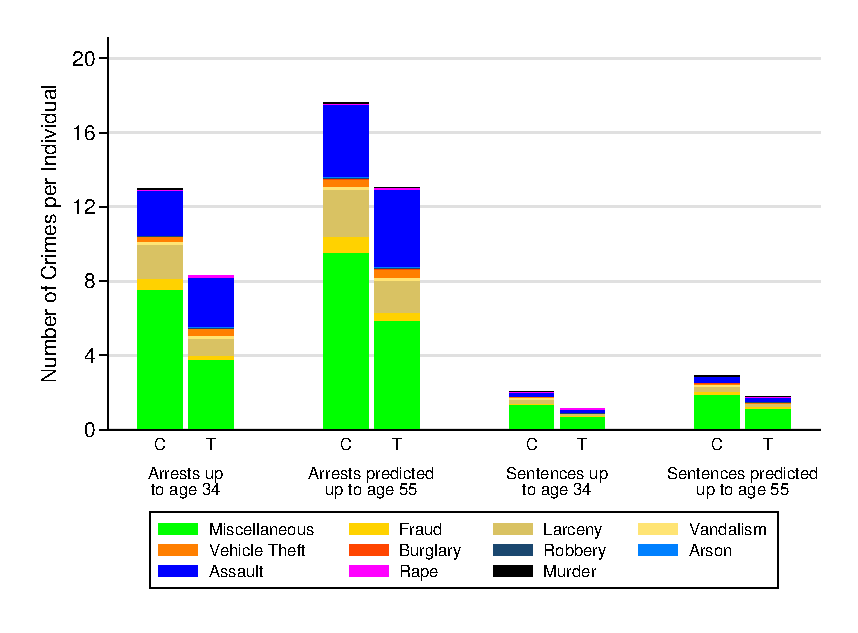
\includegraphics{AppOutput/Crime/predictions}}}
\floatfoot{
\footnotesize
\noindent Note: This figure continues Figure \ref{fig:datagraph}. It shows, for the control (C) and treatment (T) groups, the effects of adding predictions. The first pair of columns is the same as the fifth pair of columns in Figure \ref{fig:datagraph}. The second pair of columns includes the arrests that we predict. The third and fourth pairs of columns are the analogous pairs for sentences.
}\end{figure}

\subsection{Victimization Inflation}
\noindent Even though we have administrative data on crimes, we only observe the crimes that had justice system consequences (arrests or sentences). However, it is possible that the subjects committed more crimes than what we observe. Victimization Inflation (VI) is a method to capture benefits in crime reduction for crimes that did not result in justice system consequences.\footnote{\citet{Belfield_Nores_etal_2006_JHR,Heckman_Moon_etal_2010_RateofReturn}.} For most types of crimes in the US, there are many more victims than arrests or sentences. Using arrests as an example, VI assumes that those ``unpunished crimes'' were committed by the same people who were arrested for crimes of the same type, and in the same proportion. The calculation of VI uses as an input the national ratios of total number of reported crimes over the number of arrests. VI assumes that those national ratios are also valid for each individual. Under those assumptions, it is possible to find the total number of crimes committed by a subject for a given type of crime as the total number of arrests for that type of crime multiplied by the estimated national ratios for that type of crime. We estimate the total number of victims using two methods, one based on arrests and one based on sentences. Given that the ``unpunished'' crimes are by definition unobserved, it is not straightforward to use a data-driven method to allocate them between those subjects with arrests, those with sentences, and those with neither arrests nor sentences. We calculate separate estimates for arrests and sentences and use the average of those estimates as our main estimate. \\

\subsubsection{Construction of the Total Number of Victims in the U.S.}

\noindent The numerator of the VI ratio is an estimate of the total number of crimes of a certain crime type committed in the U.S. We construct this estimate using two datasets. First, we use the National Crime and Victimization Survey (NCVS). It has self-reported data on victimization of crimes reported on the household level. The data are available from 1995 to 2012. We also use the Uniform Crime Reporting Statistics (UCRS), which contains all crimes committed against households, individuals, and businesses that are reported to the police. These data are available from 1960 to 2013. Given that these two datasets independently underestimate the total number of crimes, but likely have significant overlap between them, we choose the highest estimate among both datasets for each type of crime. We refer to this estimate, $\overline{V_{j,t}}$, as the total number of victims in the country for type of crime $j$ in year $t$. \\

\subsubsection{Construction of the Total Number of Arrests in the U.S.}
\noindent The denominator of the VI ratio is an estimate of the total number of arrests of a certain type committed in the U.S. We have data from the ``National Arrests Analysis Tool'' of the National Bureau of Justice Statistics. These data are available from 1980 to 2012, which spans the years of all crimes that we observe in the ABC data. There is one problem with this dataset that we consider relatively minor: not all law enforcement agencies report the number of crimes (there are dozens of agencies that can legally arrest in the U.S.). However, as a large majority of them report the numbers of crimes, and because we are using national estimates, this should not greatly affect our calculations. We use these data to create $\overline{A_{j,t}}$, the total number of arrests in the country for type of crime $j$ in year $t$. \\

\subsubsection{Victimization Inflation Factors} 

\noindent Figure~\ref{fig:victim1} and Figure~\ref{fig:victim2} show the VI factors calculated by year. The ratios in the charts are constructed as $r_{j,t}=\frac{\overline{V_{j,t}}}{\overline{A_{j,t}}}$. In practice, we use an average of all the yearly measures in our calculations given that this exercise imputes unobserved crimes that do not have a clearly defined date. This average of all the yearly measures is given by $r_j=\Sigma_{t=t_0}^{T}r_{j,t}/T$, and has more precise estimates of the ratio. The VI factors we use for sentences are equal to the factors used for arrests, multiplied by the arrests-to-sentences ratios discussed above. Below, we will discuss combining these different estimates as per our arrest-based and sentence-based methodology. For sentences, we have data from the National Judicial Reporting Program (NJRP). These data are available from 1986 onwards. Using this dataset, we construct $\overline{S_{j,t}}$, the total number of sentences in the country for type of crime $j$ in year $t$. \\

\begin{figure} [H]
\caption{Victims-to-Arrests Ratios by Crime}
\centering \label{fig:victim1}
{\scalebox{0.8}{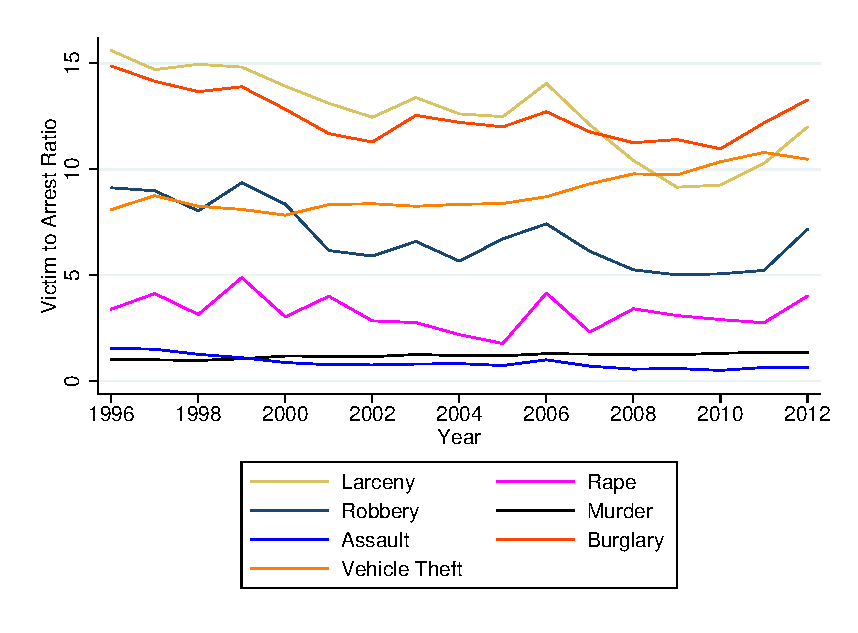
\includegraphics{AppOutput/Crime/v-to-a-ratios}}}
\floatfoot{
\footnotesize
\noindent Note: This figure shows, by year and type of crime, the number of victims (estimated from the NCVS and the UCRS datasets) divided by the number of arrests (estimated from the National Arrests Analysis Tool from the NBJS). In practice, we use a single number for each type of crime, which is an average across years.\\
}
\end{figure}

\begin{figure} [H]
\caption{Arrests-to-Sentences Ratio by Crime}
\centering \label{fig:victim2}
{\scalebox{0.8}{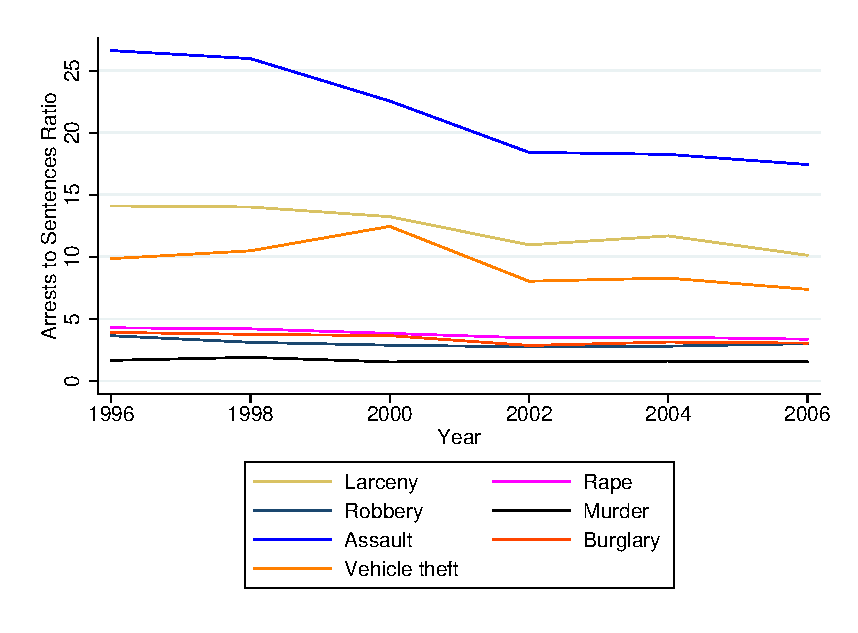
\includegraphics{AppOutput/Crime/a-to-s-ratios}}}
\floatfoot{
\footnotesize
\noindent Note: This figure shows, by year and type of crime, the number of arrests (estimated from the National Arrests Analysis Tool from the NBJS) divided by the number of sentences (estimated from the National Justice Reporting Program). In practice, we use a single number for each type of crime, which is an average across years. \\
}
\end{figure}

\subsubsection{Effects on Number of Crimes, After Victimization Inflation}
\noindent Figure \ref{fig:count-vi} shows the effects of VI on our estimates of the number of crimes committed. Note that the magnitudes in the axis are much larger than those of previous charts. The largest effects are for larceny, which is common in the data and has a victims-to-arrests factor of 12.6, the largest factor of all the categories of crime used in the paper. Given that the victim cost of larcenies is low, it affects the estimates less than what this chart suggests. \\

\begin{figure}[H]
\caption{Effects on Number of Crimes, After Victimization Inflation}
\centering \label{fig:count-vi}
{\scalebox{0.8}{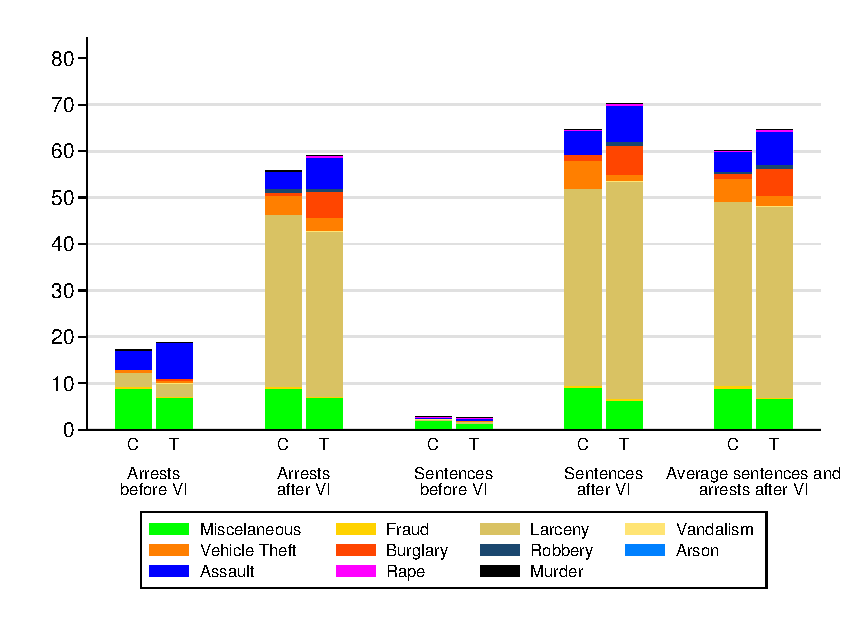
\includegraphics{AppOutput/Crime/vi}}}
\floatfoot{
\footnotesize
\noindent Note: This chart continues Figure \ref{fig:predictions}. It shows, for the control (C) and treatment (T) groups, the effects of adding victimization inflation (VI). The first pair of columns is the same as the second pair of columns in Figure \ref{fig:predictions}. The second pair of columns expand the arrests to account for VI. The third pair of columns is the same as the fourth pair of columns in Figure \ref{fig:predictions}. The fourth pair of columns expand the sentences to account for VI. The last pair of columns averages the second and the fourth pairs of columns in this chart. \\
}
\end{figure}

\noindent While the assumptions required for the victimization inflation methodology are strong, we argue that this is the best approximation for a total toll of crime's costs. The highest victims-to-arrests ratio shown in the figures are sensible and are not for the most costly categories of crime in the data, which stabilizes the estimates. \\

\subsection{Literature on Costs of Specific Crimes}
\noindent There are many methods to estimate unit costs of representative crimes, and many studies presenting estimates.\footnote{\citet{Cohen-Bowles_2010_Estimating-Cost-Crime} and \citet{McCollister_etal_2010_DAD} give comprehensive reviews of the state of the literature.} In this document, we only review the literature related to the inputs necessary for this paper. \\

\noindent We start by classifying the costs of crime, which is necessary to later discuss the methods to estimate the costs. Then, we present the two general types of methodologies that are used to estimate the total costs of crime: the Top-down methodologies and the Bottom-up methodologies. The former attempts to quantify the value that people put into \emph{ex-ante} prevention of crime, while the latter attempts to gather \emph{ex-post} all sources of costs that crime generates. The difference between these two methods can be large: \cite{Cohen-Bowles_2010_Estimating-Cost-Crime} show that for the particular case of estimates of the cost of rape, the top-down approach gives a value that is twice as large as the value given by most bottom-up studies. Other studies give cost estimates that are more homogeneous between these two approaches.\\

\subsubsection{Classifying the Costs of Crime}
\noindent Some methodologies used to estimate costs of crime are only able to capture some types of costs, and it might not even be clear what other methodologies are capturing. Some important types of costs are: \\
\begin{itemize}
\item Costs to the victim that can be directly quantified, such as medical bills, property losses, and lost productivity.
\item Costs to the victim that cannot be observed, such as pain and suffering.
\item Costs to the community in terms of prevention of crime, such as alarms, avoidance behavior, and police presence.
\item Costs to the community in terms of fear.
\item Costs to the community in terms of the criminal justice system, especially imprisonment.
\item Costs to the offender in terms of lowered productivity, such as forgone wages.
\end{itemize}

\subsubsection{Bottom-up (BU) Methodologies}
\noindent These approaches sum each type of cost that is imposed after the crime has been committed. The most well-known studies combine direct (also known as tangible) costs of the crimes with intangible costs. Tangible costs are everything that can be directly measured by observation, such as foregone wages, hospital costs, and police expenditure. Intangible costs are subjective, like pain and suffering. One way to measure these costs is using jury awards. For example, a jury award given as a result of an arm broken at a construction site can be used as a proxy of the intangible cost of having an arm broken in an assault.\footnote{This was first used in \citet{cohen_1988_Pain-Suffering}, and has been extensively used in BU studies after that. \citet{Miller_Cohen_ea_1996_BOOKvictim} improved on previous estimates by using jury awards specifically coming from criminal cases.} The problem of these approaches is that many of the costs of crime are not directly imposed on the victim and are hard to quantify, such as the ``fear of crime,'' the increased expenditure on crime prevention, and the negative impact of imprisonment on the community. \\

\subsubsection{Top-down (TD) Methodologies}
\noindent The other way to estimate the cost of crime is using TD methods, based on eliciting willingness to pay for avoiding crimes. The main advantage of these methods is that, in principle, they consider costs that are hard or impossible to measure directly, such as the cost of fear, avoidance behavior, and expenditures in preventative measures. There are three main methodologies for this approach, which we now briefly describe. \\

\begin{enumerate}
\item Stated Preferences. This basic method elicits the willingness to pay for hypothetical programs that would reduce crime nationwide for a sample of people.\footnote{\citet{Cohen_Rust_etal_2004_Criminology}.} Being an example of a TD methodology, it is expected that the costs obtained by this method would include factors that affect the community, and that are hard to capture, such as fear. However, it is unclear whether people consider factors like the cost of the justice system in their answers to these questions. An obvious caveat of this method is that people might not answer the real amount they would be willing to pay in these surveys.
%Then, multiplying that willingness to pay by the number individuals that would contribute, the total WTP for a certain reduction in crime is obtained. Dividing that total WTP by the number of crimes that would be avoided (number of crimes committed times the hypothetical effectiveness of the program), it is possible to find the WTP to avoid a particular crime.
\item Revealed Preferences. This method infers the value that individuals assign to crime reductions from market transactions. The most standard way to calculate these estimations is running regressions to explain the total price of houses with several factors, including the rates of crime in the area. Those parameters associated with the crime rate are considered the revealed valuation of avoiding crimes.\footnote{\citet{Thaler_1978_Value-Crime-Control}.} One weakness of this method is that it assumes that people are well-informed on the crime rates in an area. Another problem is that, in absence of extremely large and rich data on crimes and housing prices, it is not possible to separately identify the costs of different types of crimes. To the best of our knowledge, no paper has yet been able to convincingly obtain estimates per type of crime with this method.
\item Life Satisfaction. For this method, people are surveyed about their preferences between different life conditions, in which several different factors are considered. Some of those factors are income and rates of crime. By doing so, people implicitly associate monetary values to the levels of crime in the communities they would live in.\footnote{\citet{ Moore_etal_2006_Cost-of-Fear,Moore_2006_Value-Reducing-Fear}.}
\end{enumerate}

\subsubsection{Costs Used in this Study}
\noindent To summarize, both approaches have strengths and weaknesses: the TD approaches are more likely to reflect costs to the community (e.g. fear and anxiety, avoidance behavior, and protective measures) and better capture the spirit of a prevention program. However, in practice TD estimates rely on strong assumptions, and there are methodological issues associated with obtaining detailed values for the different types of crimes. It is also possible that when people answer the survey used for TD calculations they include some costs that we are including separately, such as justice system costs, and risk of death from non-murder crimes, while BU does not include them. Given those considerations, and the lack of TD costs for some categories of crime, we use BU costs for our main estimates. For completeness, we present cost estimates using both approaches. We choose \cite{Cohen_Rust_etal_2004_Criminology} as representative of the TD approaches, and \cite{McCollister_etal_2010_DAD} as representative of the BU approaches. In terms of timing, both of these studies match well with the ABC data. The bulk of crimes in the ABC data occurred between the late 1990s and early 2000s. While \cite{Cohen_Rust_etal_2004_Criminology} do not report the exact year of their survey, they use Census 2000 figures for their estimates. Even though \cite{McCollister_etal_2010_DAD} is a more recent study, many of the productivity estimates that their costs are based on are taken from papers using data from years with more crimes the late 1990s and early 2000s. The costs in those studies are presented in Table \ref{tab:individual-crime-cost}. Notice that there are some strong differences in the cost of crimes, such as assault, burglary, and especially robbery. \\

%The fact that \cite{cohen1994costs} and \cite{miller1996victim} are relatively old studies is an advantage rather than a problem. The studies better reflect the costs of crimes in those years, which are part of the period in which most crimes were committed by subjects in the ABC data. More recent estimates will be based on assumptions about productivity and costs that are not representative of the losses relevant for this study. These studies are complementary, as \cite{miller1996victim} quantifies cost to victims (productivity, medical care, mental health care, police/fire services, social services, property loss and quality of life damages), while \cite{cohen1994costs} provides a quantification of criminal justice system costs. Importantly, this study distinguishes between sources of costs, so we can impute our own cost estimates to sentences, knowing precise information about time in jail for our sample. The most recent study  \citep{mccollister2010cost} is necessary because it considers some types of crimes omitted in the previous papers.

\begin{table}[H]
\begin{threeparttable}
\caption{Unitary Costs of Crime for Victims} \label{tab:individual-crime-cost}
\begin{tabular}{lcc}
\toprule
Crime				&Top-Down Approach	&Bottom-Up Approach	\\
					& \cite{Cohen_Rust_etal_2004_Criminology}&\cite{McCollister_etal_2010_DAD}\\ \midrule
Arson				&					&12,093			\\
Assault				&95,200			&16,132 			\\
Burglary			&34,000			&1,467 			\\		
Fraud				&				&0				\\
Larceny				&				&528 				\\
Motor Vehicle Theft	&				&6,699 			\\
Murder				&13,192,000		&9,286,200 		\\
Rape				&322,320			&224,021 			\\
Robbery				&315,520			&7,273 			\\
Vandalism			&					&0				\\ \bottomrule
\end{tabular}
\begin{tablenotes}
\item Note: All amounts are in 2014 USD. The amounts reported in \cite{McCollister_etal_2010_DAD} for non-murder crimes have the extra cost for risk of death and the cost of a crime career removed (both were obtained from correspondence with the author). Risk-of-death costs do not apply, because we know the outcomes of the crimes. Crime-career costs do not apply, as we directly observe the income of the individuals. These costs also don't include police and legal system costs, as those are imputed separately and only for the cases for which individuals were arrested or sentenced.
\end{tablenotes}
\end{threeparttable}
\end{table}

\subsubsection{Timing of Effects: Incidence vs. Prevalence}
\noindent We would like to discount the costs of crime according to whether they were \textit{incurred} during a particular age of ABC subjects, because those values should be discounted at a different rate than costs incurred later, even if both costs were \textit{imposed} in the same year. Thus, the value of the imprisonment is discounted year-by-year. We have no information about the timing of costs for victims, so the value of the different crimes for the victims are discounted according to the time they were imposed (the time of the crime's occurrence). \\

\subsubsection{Costs of Imprisonment}
\noindent Unlike previous studies, we observe the sentences of the ABC participants. This allows for a precise estimation of the costs of imprisonment. For the cost of jail and state prison, we use estimates from the \citet{US-Justice_1988_Report-Crime-Justice}. In 2014 USD, these costs are \$25,338 for a year in a state prison, and \$21,939 for a year in jail.
It is important to clarify that we only include costs of the justice system for the crimes that are known by the justice system, not for the crimes that we impute through victimization inflation. \\

%%%%%%%%%%%%%%%%%%%%%%%%%%%%%%%%%%%
\subsection{Effects on Costs of Crime}

%\subsubsection{Criminal Behavior.} The results show that there are clear reductions in the amount of crime committed between the control and treatment groups. This holds true for the majority of the categories of crime. The exceptions were Vehicle Theft, Assault, Robbery, and Arson. The visualization of the ABC data in Figure \ref{tab:lifehistory} represents the life history of each of the individuals within the ABC study that committed at least one crime, with each dot as an offense and each line as a period of incarceration. Also shown are the most serious crimes committed in the ABC data, including a habitual felon, manslaughter, and indecent liberties with children. The largest treatment effects occurred in cases of Miscellaneous, Fraud, and Larceny crimes. In sentences alone, there was a 46.3\% reduction in the number of cases, and in arrests, there was a 39\% reduction in cases for those in the treatment group compared to the control group. There are substantially fewer arrests for the individuals in the treatment group, and although there are still a few who committed a series of crimes, many did not have arrests at all.
%numbers from combined_datasetv3

\subsubsection{Effects on Costs Before Victimization Inflation}  Figure \ref{tab:diff-costs} presents the estimated costs per type of cost before victimization inflation.
\noindent There are clear positive effects for the treatment group in terms of reductions in the costs of crime. Those reductions are almost exclusively given by the large effect of the murder case we observe in the control group (note that murder also appears in the treatment group costs because of the predictions). Comparing the bars in this figure, the costs from the justice system and from imprisonment are low compared with the victimization costs, even without victimization inflation. While the levels of the arrest-based estimates are higher than the levels of the sentence-based estimates for both the treatment and control groups, the impacts of the program are quite similar across both methods (Figure~\ref{tab:diff-costs}). \\

\begin{figure} [H]
\caption{Costs of Crime Before Victimization Inflation}
\centering  \label{tab:diff-costs}
{\scalebox{0.8}{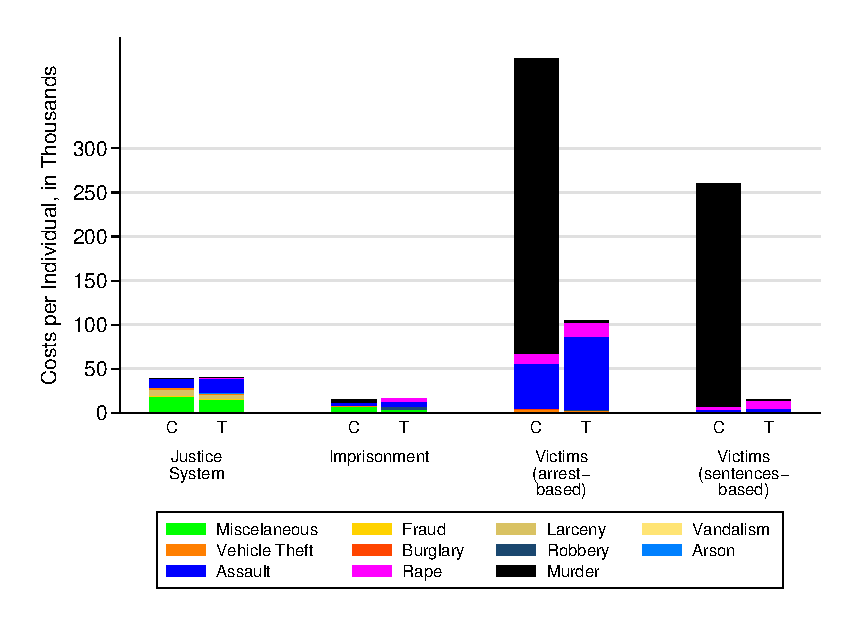
\includegraphics{AppOutput/Crime/different_costs}}}
\floatfoot{
\footnotesize
\noindent Note: This figure depicts the per capita cost for the different categories of costs and crimes we use, by control (C) and treatment (T). The first pair of columns adds up the justice system costs (including police) for all arrests inputed for each subject. The second pair of columns adds up the cost of Imprisonment. It is important to note that the costs are per capita, so there are individual cases that have much higher costs. The next two pairs of columns show the pre-victimization inflation estimates of number of crimes multiplied by the individual victim cost of the different crimes. The costs are taken from the Bottom-up approach in Table \ref{tab:individual-crime-cost}. All costs are in thousands of 2014 USD.\\
}
\end{figure}

\subsubsection{Effects on Costs After Victimization Inflation}

\noindent Figure \ref{tab:costs_vi} presents the data after applying the victimization inflation. As shown below, the inflation allows us to include a substantial amount of crime that otherwise would not have been considered. This chart shows that the treatment effects using arrest-based estimations are not substantively different from the ones using sentence-based estimations. Thus, to use all available information, we use the estimates based on the averages of the two for our analysis. \\

\begin{figure} [H]
\caption{Costs of Crime After Victimization Inflation}
\centering  \label{tab:costs_vi}
{\scalebox{0.9}{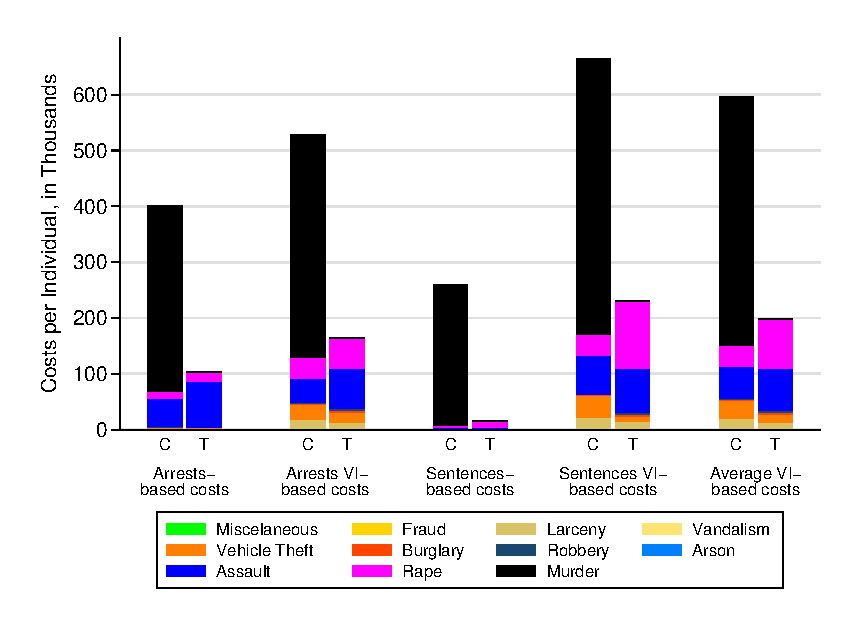
\includegraphics{AppOutput/Crime/costs_vi}}}
\floatfoot{
\footnotesize
\noindent Note: This figure depicts the per capita cost for the different categories of costs and crimes we use, by control (C) and treatment (T). The first two pairs of columns adds up all of the arrest-based costs for each subject and compares the pre- and post-victimization inflation costs. The third and fourth pair of columns compare the pre- and post-victimization inflation sentence-based costs. It is important to note that the costs are per capita, so there are individual cases that have much higher costs. The next two pairs of columns show the post-victimization inflation estimates of number of crimes multiplied by the individual victim cost of the different crimes. The costs are taken from the Bottom-up approach in Table \ref{tab:individual-crime-cost}. All costs are in thousands of 2014 USD.\\
}
\end{figure}

\noindent We consider the impact on murder as a consequence of the program rather than a statistical coincidence. We use as precedent the cost-benefit analysis of Perry in which three control group individuals and one treatment group individual committed murders.\footnote{\citet{Heckman_Moon_etal_2010_RateofReturn}.} \\

Some of the sources of cost estimates, such as the more serious crimes, result in volatile estimates due to the small sample sizes. Our estimations of the standard errors associated with the objects of interest in this paper---the present value of the program and the internal rate of return---consider those sources of volatility. Ultimately, the benefit-cost analysis is a unidimensional summary of benefits of a program, and specific flows of benefits with high variability enter naturally into the process of aggregation. \\

%\begin{table}[H]
%\begin{threeparttable}
%\caption{Effects on Total Costs}\label{tab:apx_impact-costs-total}
%{
\def\sym#1{\ifmmode^{#1}\else\(^{#1}\)\fi}
\begin{tabular}{l*{1}{ccccc}}
\hline\hline
                    &Mean Control&Mean Treatment&  Difference&           $t$& $p$-value\\
\hline
Total Costs for All Crimes&      246967&      150511&       96456&        0.64&        0.26\\
Costs Miscelaneous  &       14769&        8058&        6711&        1.45&       0.075\\
Costs Fraud         &        1095&         635&         460&        0.79&        0.21\\
Costs Larceny       &       11793&        7910&        3883&        0.83&        0.20\\
Costs Vandalism     &         260&         193&          67&        0.43&        0.34\\
Costs Vehicle Theft &       14866&       10327&        4540&        0.39&        0.35\\
Costs Burglary      &        1253&         291&         962&        1.36&       0.088\\
Costs Robbery       &        1091&        4500&       -3408&       -1.13&        0.87\\
Costs Arson         &         161&         152&          10&       0.093&        0.46\\
Costs Assault       &       38830&       33484&        5346&        0.30&        0.38\\
Costs Rape          &       35388&       65721&      -30333&       -0.43&        0.67\\
Costs Murder        &      127460&       19242&      108218&        0.87&        0.19\\
\hline\hline
\end{tabular}
}

%\begin{tablenotes}
%\item  Note: this table presents the treatment effects of ABC on total costs of crime per capita, including Victimization Inflation. All costs are in 2014 USD. We present one-sided $p$-values.
%\end{tablenotes}
%\end{threeparttable}
%\end{table}

\subsection{Sensitivity Analyses Using Alternative Cost Estimates}
\noindent So far, we study several ways to construct our estimates: \\

\begin{enumerate}
\item We show that not matching the different crime datasets could reduce the number of crimes, but that the general patterns are stable, and no dataset is especially influential.
\item We show that not including predictions up to age 50 noticeably reduces the number of crimes, but the general patterns are not modified.
\item We show estimates using arrest-based estimations versus sentence-based estimations, and find that the differences are large in terms of the number of crimes before victimization inflation, but small after it, and do not substantially change the total benefits calculations.
\end{enumerate}

\noindent In Figure \ref{fig:costs_schedules}, we present additional deviations from our main estimates. In particular, we show how the estimations change when two different cost schedules are used: (i) Top-down costs, and (ii) Bottom-up costs, assuming that the costs of murders and rapes are identical to the cost of an assault. We also note that BU costs are a ``conservative'' option in the sense that the effects of the program are higher using TD costs. We can also see that with no murders and rapes, the effect of the program on crime is still positive, but much smaller than when those crimes are considered. \\

\begin{figure} [H]
\caption{Different Cost Schedules}
\centering  \label{fig:costs_schedules}
{\scalebox{0.9}{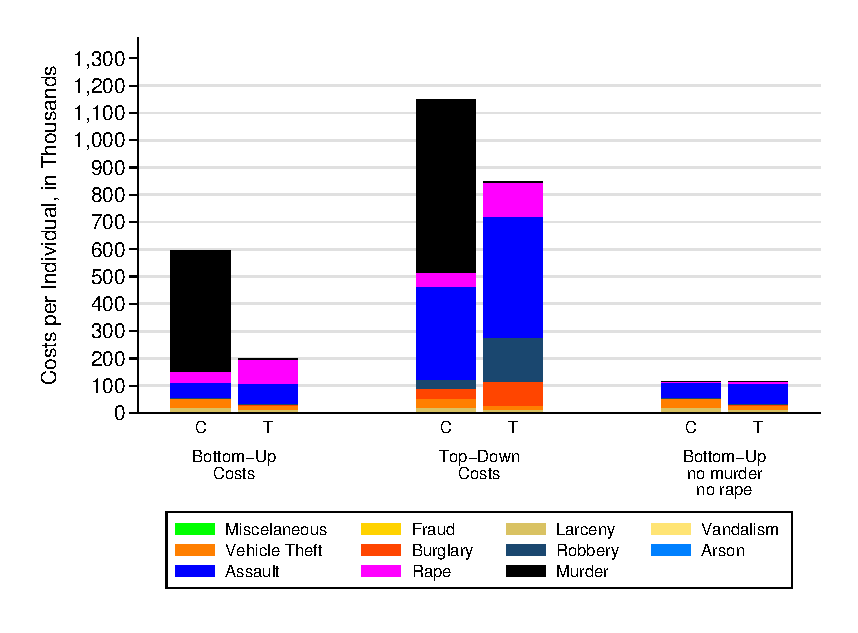
\includegraphics{AppOutput/Crime/bu_td_nomur}}}
\floatfoot{
\footnotesize
\noindent Note: This figure depicts the per capita cost for the different categories of costs and crimes we use, by control (C) and treatment (T). It presents some sensitivity analyses. The first pair of bars represents costs using the Bottom-up approach in Table \ref{tab:individual-crime-cost} to determine individual costs of crime. The second pair of bars represents costs using the Top-down approach in Table \ref{tab:individual-crime-cost} to determine individual costs of crime. The third pair of bars uses the Bottom-up approach, but replaces the values of murders and rapes with that of assaults.\\
}\end{figure}

\noindent Finally, in Figure \ref{fig:crime_discounting}, we present the effect that discounting and applying deadweight loss has on our estimates. The first pair of bars represents the cost estimates that are not discounted, the second pair of bars represents the discounted costs, and the third pair of bars represents the discounted costs including deadweight losses. It is clear that the effect of discounting is substantial, approximately halving the total cost estimates. The effect of applying deadweight loss barely changes the estimates. The effect of deadweight loss is most noticeable in the value of miscellaneous crimes, which are only public costs. Regardless, its impact in the overall costs is minor. \\

\begin{figure} [H]
\caption{Effect of Discounting Crime Costs}
\centering  \label{fig:crime_discounting}
{\scalebox{0.9}{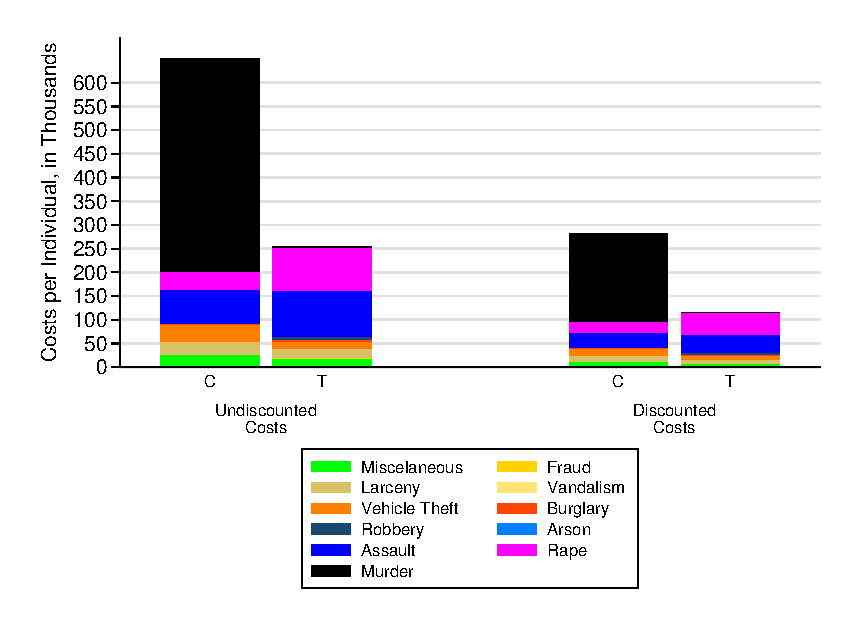
\includegraphics{AppOutput/Crime/crime_discounting}}}
\floatfoot{
\footnotesize
\noindent Note: This figure depicts the per capita cost for the different categories of costs and crimes we use, by control (C) and treatment (T). The discounted costs use 3\% as a discount factor, and are discounted to birth. The deadweight loss (DWL) adjustments increases the costs from justice system and imprisonment by 50\%. All costs are in thousands of 2014 USD.\\
}\end{figure}


\setcounter{figure}{0}  \renewcommand{\thefigure}{L.\arabic{figure}} % anna note: note there are two income appendices
\setcounter{table}{0}   \renewcommand{\thetable}{L.\arabic{table}}
\section{Interpolation of Parental Income}
\label{app:parent_income}


\noindent We observe labor income of the mother and, if applicable, her partner at
ages 0, 2, 3, 4, 5, 9, 12, and 15. To obtain our measure of parental income, we simply
sum the labor income of the respondent and her partner. \\

% Income of the parents of ABC subjects is observed at ages 2, 3, 4, 5, 9, 12, and 15.
% For ages 2 to 9, we observe only the annual income of parents, which we use in our
% estimates. The data do not distinguish the source of the annual income. Thus,
% it is unclear whether those variables are pre- or post-tax, and if they include
% transfers, income from additional contributors, or are restricted to labor income.
% At age 9, data on parent income are collected twice, so we use the average of the
% reported incomes.

% At age 12, in addition to observing annual income of parents,
% we also observe income from transfers, which includes child support, disability
% benefits, food stamps, rent subsidies, social security, and other sources of government
% transfers. As it is unclear whether or not the data we observe on annual parent income
% includes government transfers, we construct our variable for parent income at
% age 12 by taking the midpoint between annual parent income and annual parent income summed
% with income from transfers.

% At age 15, we observe annual earned income of parents, in addition to income from food
% stamps, rent subsidies, social security, AFDC, child support, and other government transfers.
% To construct parent income at age 15, we sum all the components above.

% At all ages, income from other family members are excluded, and all values are inflated
% to 2014 dollars.

\setcounter{figure}{0}  \renewcommand{\thefigure}{K.\arabic{figure}}
\setcounter{table}{0}   \renewcommand{\thetable}{Ks.\arabic{table}}
\section{Extrapolation of Individual Income}
\label{app:subject_income}

\subsection{Data Sources}

\noindent Income of the ABC and CARE subjects is observed in detail at ages 21 and 30. For both ages,
we separate labor income from public-transfer income. At age 21, public-transfer income includes Aid to
Families with Dependent Children (AFDC) subsidies, food stamps, survivor benefits, disability
benefits, social security, rent subsidies, and fuel subsidies. At age 30, public-transfer income includes food stamps, welfare, housing assistance, workman's
compensation, disability, social security, supplemental security income, unemployment benefits,
worker's compensation insurance, fuel subsidies, educational and aid grants, and other forms of welfare.
At both ages 21 and 30, labor income is observed. Also at both ages, income from other family members are excluded, and all values are in
to 2014 USD. We utilize the
NLSY, CNLY, and PSID datasets. We provide a brief overview of them below. \\

\subsubsection{NLSY}
\label{app:subject_income_nlsy}

\noindent The National Longitudinal Survey of Youth (NLSY) is a longitudinal survey beginning in 1979
that follows individuals born between 1957 and 1964. The initial interview included
12,686 respondents aged 14 to 22. The survey was designed to include 6,111
individuals representing the non-institutionalized civilian population, a supplemental
sample of 5,295 civilian Hispanics, Latinos, blacks, non-blacks/non-Hispanics, and economically
disadvantaged youth, and a sample of 1,280 who served in the military as of September 30,
1978. When appropriately weighted, the NLSY is nationally representative of the youth
living in the U.S. on January 1, 1979. We include individuals from all three subsamples
in our analysis. \\

\noindent The NLSY collected data on labor market participation, education, family background,
family life, health issues, assets and income, government program participation, and
measures of cognitive skills. We use these data to estimate a prediction model for
subject income for ages 31 through 67. \\

\noindent We restrict the NLSY sample to individuals with labor income less than
\$300,000 (2014 USD) at any given year. With the mean labor income (2014 USD) in the ABC
sample being \$12,232 at age 21 and \$32,782 at age 30, and the maximum reported
being \$189,938, the cut-off we impose on the auxiliary data is high enough
so that everyone in the ABC  and CARE samples are represented, yet low enough to
exclude high-earning individuals in the auxiliary sample that do not reflect the ABC or CARE samples well. \\

\noindent We do not impose a restriction on birth year on the NLSY as all respondents are aged between 47 and 55
at the time of the last interview (conducted in 2012). This age range is within the 31--67 range for which
we extrapolate the income of the ABC and CARE subjects. \\

\noindent Given the biennial nature of the NLSY, we only observe each subject at either odd or even
ages. Not only does this reduce the size of the sample on which we fit our prediction model
at each age, but it can introduce biases associated with the odd-aged and even-aged cohorts.
To address this issue, we perform a linear interpolation on the variables in the NLSY data
that enter into our prediction model. This allows us to estimate our prediction model on
all subjects of the NLSY satisfying our restrictions at every age. \\

\subsubsection{CNLSY}
\label{app:subject_income_cnlsy}

\noindent The Children of the National Longitudinal Survey of Youth (CNLSY) is a survey of the children of the mothers from the NLSY, beginning in 1986. At the time of
the initial interview, the ages of the children surveyed ranged from 0 to 23. As of 2010,
the CNLSY sample includes 11,504 children born to NLSY mothers. With appropriate weights,
the CNLSY may be considered nationally representative of children born to women
who were aged 14 to 22 during 1979. Interviews were conducted annually between 1986 and 1994,
and biennially thereafter. \\

\noindent Similar to the NLSY, the CNLSY collected data on cognitive ability, motor and social development,
home environment, health information, education, attitudes, employment, income, family decisions,
and more. We use these data to estimate a prediction model for subject income for ages
22 through 29. \\

\noindent As we did with the NLSY, we restrict the CNLSY sample to individuals with labor income less than
\$300,000 (2014 USD) at any given year. In addition to this, we limit the sample to subjects born
between 1978 and 1983. Because the CNLSY data extend to 2012, this implies that we use the most
recent data from the CNLSY in which individuals are aged 29 to 34. Finally, given the biennial
nature of the survey, we perform a linear interpolation on the variables that enter into our prediction
model. This allows us to use as much of the CNLSY data as possible at every age when
interpolating subject income. \\

\subsubsection{PSID}
\label{app:subject_income_psid}

\noindent The Panel Survey of Income Dynamics (PSID) is a longitudinal household survey containing between 5,000
and 8,500 families in each wave. It began as yearly survey in 1968 and has been fielded biennially since 1996.
When appropriately weighted, the PSID is designed to be representative of U.S. households. The PSID
provides extensive information concerning demographics, economic outcomes, health outcomes, marriage
and fertility, and more. In addition to using the PSID to forecast future earnings of ABC and CARE subjects, we
use the PSID to forecast health outcomes. See Appendix \ref{section:data_psid} for details on how the
PSID relates to health outcomes. \\

\noindent Similar to the CNLSY, we restrict the PSID to individuals born between 1945 and 1981. Because the data
extend to 2013, this means we use the most recent subsample of individuals aged 30 to 67.
We also exclude all individuals with labor income exceeding \$300,000 (2014 USD) at any given year.
Finally, given the biennial nature of the survey, we perform a linear interpolation on the variables
that enter into our prediction model. This allows us to use as much of the PSID data as possible at
every age to interpolate subject income. \\



\setcounter{figure}{0}  \renewcommand{\thefigure}{N.\arabic{figure}}
\setcounter{table}{0}   \renewcommand{\thetable}{N.\arabic{table}}
\section{Forecasting Health Outcomes Using the Future Adult Model (FAM)} \label{appendix:health}

In this paper, we also forecast and monetize health outcomes for treatment and control individuals. When studying labor income, a first-order autoregressive model suffices to make valid forecasts. When forecasting health, a richer model conditioning on multiple health conditions is required to make valid forecasts. We use a dynamic microsimulation model (the Future Adult Model - FAM) as a vehicle for forecasting health-state occupancy probabilities and associated benefits and costs. Using this tool, we forecast the health trajectories of the ABC/CARE individuals. To forecast health, we use a comprehensive ABC/CARE age-30 health interview and a health follow-up conducted when the subjects were in their mid-30s to initialize the forecast of their health trajectories. We then monetize health outcomes using quality-adjusted life years and medical costs.\footnote{The  microsimulation model that we use is an extension of the model used by \citet{Prados_etal_2015_How-Much-Can-Education}. Technical details are described in \citet{Goldman_etal_2015_Future-Adult-Model}. Both models are related to the Future Elderly Model (FEM), which is a microsimulation tool originally developed to examine the health and health care costs among the elderly Medicare population \citep{Goldman_etal_2004_RAND-Report_Health-Status-Elderly}. It has been used extensively to assess health and disease prevention scenarios: FEM has been used to assess the future costs of disease, the benefits of preventing disease among older population, the consequences of new medical technologies, trends in disability, and the fiscal consequences of worsening population health (see \citet{Goldman_etal_2004_RAND-Report_Health-Status-Elderly}, \citet{Lakdawalla_etal_2004_Health-and-Cost}, \citet{Goldman_etal_2005_HA}, and \citet{Zissimopoulos_etal_2014_Delaying-Alzheimers}). The main differences of FAM with FEM are that the model we use starts with cohorts of individuals at age 30 instead of 50, and that it simulates more outcomes than FEM. These additional outcomes are useful in explaining health outcomes and medical expenditure at younger ages. For example, we analyze the evolution of partnership and marital status, work status, and family size.} Before providing formal details, we summarize the data sets used, as well as variable construction and imputation assumptions. 

\subsection{Data Sources} \label{section:data}
\noindent FAM uses data from ABC/CARE follow-up surveys to build the initial state of the cohort. 
The transition model parameters are estimated from the 1997 to 2013 waves of the Panel Study of Income Dynamics (PSID). 
We supplement the PSID with data from the Health and Retirement Study (HRS). We use the National Health and Nutrition Examination Survey (NHANES) 
to account for differences between measured and self-reported BMI.
To estimate medical care costs associated with health conditions, we use the Medical Expenditures Panel Survey (MEPS) and the Medicare Current Beneficiaries Survey (MCBS). \\


\subsubsection{PSID}
\label{section:data_psid}
%The Panel Survey of Income Dynamics (PSID) is a longitudinal household survey containing between 5,000 and 8,500 families in each wave, which began yearly in 1968 and is fielded biennially since 1996. When appropriately weighted, the PSID is designed to be representative of U.S. households. The PSID provides extensive information concerning demographics, economic outcomes, health care access, health outcomes, and health behaviors (such as smoking history, alcohol consumption, and exercise habits). Health outcome variables include diagnosis of diabetes, heart disease, hypertension, lung disease, cancer, etc. 

\noindent The Panel Study  of Income Dynamics (PSID) provides extensive information concerning demographics, economic outcomes, health care access, health outcomes, and health behaviors (such as smoking history, alcohol consumption, and exercise habits). Health outcome variables include diagnosis of diabetes, heart disease, hypertension, lung disease, and cancer, among others.\\

\noindent We estimate the transition models using waves from 1997 to 2013. We create a dataset of respondents who have formed their own households, either
as single heads of households, cohabiting partners, or married partners.  These heads, wives, and husbands respond to the richest
set of PSID questions, including the health questions that are critical for our purposes. We use all respondents aged 25 and older.\footnote{While we use the full sample, we explored using a few different subsamples to better adapt to the demographics of the ABC/CARE subjects.}  
The length of the PSID is a significant advantage, because we can include past health behaviors as explanatory variables for current health outcomes. This dataset provides adequate sample sizes to explore health outcomes of specific groups. 
PSID does not follow individuals who are institutionalized in nursing homes or other long-term care facilities. To overcome this weakness, we pool the PSID sample with the HRS sample when
estimating mortality models. \\

\subsubsection{HRS}

\noindent The Health and Retirement Study (HRS) is a longitudinal panel that surveys a nationally representative sample of individuals over the age of 50 and their spouses every two years.  When appropriately weighted, the HRS in 2010 is representative of U.S. households 
where at least one member is at least 51 years old.
This study collects in-depth information about income, work, health, and medical expenditures. In our model, waves from 1998 to 2012 are pooled with the PSID for estimation of mortality and 
widowhood models. The HRS data
are harmonized to the PSID for all relevant variables. Because PSID does not follow respondents into nursing homes, we also use the HRS to estimate the model for nursing home residency.  We use all cohorts in the dataset created by RAND (RAND HRS, version O) as the basis 
for our analysis. \\

\subsubsection{MCBS}
\noindent The Medicare Current Beneficiary Survey (MCBS) is a nationally representative sample of aged, disabled, 
and institutionalized Medicare beneficiaries.  The MCBS attempts to interview each respondent twelve 
times over three years, regardless of whether he or she resides in the community, a facility, or 
transitions between community and facility settings. The disabled (under 65 years of age) and 
very elderly (85 years of age or older) are over-sampled. The first round of interviewing was conducted 
in 1991. Originally, the survey was a longitudinal sample with periodic supplements and indefinite 
periods of participation. In 1994, the MCBS switched to a rotating panel design with limited periods 
of participation. Each fall, a new panel is introduced, with a target sample size of 12,000 respondents. Each summer, a panel is retired. Institutionalized respondents are interviewed by proxy.  The MCBS 
contains comprehensive self-reported information on the health status, health care use and 
expenditures, health insurance coverage, and socioeconomic and demographic characteristics of the 
entire spectrum of Medicare beneficiaries.  Medicare claims data for beneficiaries enrolled in 
fee-for-service plans are also used to provide more accurate information on health care use and 
expenditures.  MCBS data from 2007 to 2010 are used for estimating medical costs and enrollment models. \\

\subsubsection{MEPS}
\noindent The Medical Expenditure Panel Survey (MEPS), which began in 1996, is a set of large-scale surveys of families and individuals, their medical providers, and employers across the U.S. The Household Component (HC) of the MEPS provides data from 
individual households and their members, which is supplemented by data from their medical providers. 
The HC collects data from a representative subsample of households drawn from the 
previous year's National Health Interview Survey (NHIS). Since NHIS does not include the 
institutionalized population, neither does MEPS; this implies that we can only use the MEPS to 
estimate medical costs for the non-elderly (ages 25--64) population. Information collected during household 
interviews include: demographic characteristics, health conditions, health status, use of medical 
services, sources of medical payments, and body weight and height. Each year the household survey 
includes approximately 12,000 households, or 34,000 individuals. Sample size for those aged 25-64 is 
about 15,800 in each year.  MEPS has comparable measures of socioeconomic status as those in PSID, 
including age, race and ethnicity, educational attainment, census region, and marital status.  We estimate medical expenditure 
and utilization using data from 2008 to 2010. We use waves from 2001 to 2003 to estimate models of quality-adjusted life years (QALYs), due to availability of EQ-5D instrument in these waves.\footnote{Section \ref{section:FAM_models} explains the estimation of the QALY model.} \\


\subsubsection{NHANES}
\noindent 
The National Health and Nutrition Examination Survey (NHANES) targets a nationally representative sample of approximately 5,000 individuals in each year since 1999.  The data collected includes responses to interview questions about demographics, disease conditions, height, and weight, as well as physical measurement of BMI.  We use NHANES years 2002 to 2010 to estimate a model for imputing measured BMI from self-reported BMI.  The methodology is described in Section \ref{section:FAM_ABC_impute}.

\subsubsection{ABC/CARE}
\noindent FAM uses ABC/CARE data to initialize the state of each ABC/CARE subject when they enter into the simulation.  
These data are taken from the the parental interviews at various subject ages from birth to age 21; age-30 subject interview; and mid-30s biomedical survey.  
The goal is to have each subject's initial state in the simulation match their status at the age-30 subject interview. However, because several key FAM inputs are not available at the age-30 interview, we use PSID or ABC/CARE surveys corresponding to other ages to impute missing elements. These imputations are discussed in Section \ref{section:FAM_ABC_impute}. \\

% \todo we could add a table of all the FAM input variables (rows) and three columns, as-is, rule imputed, model imputed, with checkmarks to indicate how the data were derived

\subsection{Methods and Analysis}

\subsubsection{ABC and CARE Data Assumptions and Imputations}
\label{section:FAM_ABC_impute}

% \todo would be nice to have a table that summarizes imputed variables at age 30, imputation method, and number of missing subjects

\noindent Marital status transitions and childbearing in FAM are affected by the subject's mother's education level. The ABC and CARE age-30 subject interview did not ask about mother's education, but the ABC age-21 parent interview did.
For ABC subjects, we assume that each subject's mother had the same education level at the age-30 subject interview as what was reported in the age-21 parent interview. For CARE subjects, we impute mother's education from an ordered Probit model using race, ethnicity, education, disease conditions, employment status, presence of a health-related work limitation, and a self-report of whether or not the subject was ``poor'' as a child.  The model is estimated using age 30 to 31 PSID subjects.  Each of the model covariate values are taken from the CARE age 30 interview. At the beginning of each simulation repetition, an education level is randomly drawn from the probability distribution for each CARE subject and assigned to be the mother's education level.  \\

\noindent Many FAM transition models depend on a three-level measure of parents' economic status when the subject was a child.
This is based on the PSID question: ``Were your parents poor when you were growing up, pretty well off, or what?''
The three possible responses are ``poor,'' ``average''/``it varied'', or ``pretty well off.''
This question is not included in the ABC or CARE interviews, but because preliminary eligibility for the program focused on children from high-risk backgrounds, based on socioeconomic factors, the value of this variable is set to ``poor'' (when growing up) for all ABC and CARE subjects. \\

\noindent All FAM transition models depend on demographics of the subject, including whether or not the subject is Hispanic.
This information is not available in the ABC or CARE data, but it is assumed that none of the ABC or CARE subjects are Hispanic.\footnote{Census data on Hispanics in North Carolina were not available for 1970 and 1980, but Hispanic migration into this state is more recent than in other regions, and as late as 1990, only 2\% of the North Carolina poor were Hispanic \citep{Johnson_2003_Changing-Poverty}.} \\

\noindent Most FAM models depend on smoking status. Employment status affects FAM transitions in marital status, childbearing, claiming of disability insurance (DI) and supplemental security income (SSI), and type of health insurance.
One male in the ABC control group was missing smoking status and, although known to be not working, was also missing specific employment status (unemployed or out of the labor force).
 We use a multinomial logit model to jointly estimate the probability of each combined smoking and employment category among 25- to 35-year-olds in the PSID who were not working. At the beginning of each simulation repetition, we use a Monte Carlo random draw generated from this distribution to assign this subject's smoking and employment statuses. This same subject is also missing information about binge drinking.  A separate binary Probit binge drinking model was estimated using the age 25--35 PSID data. A Monte Carlo random draw is taken according the Probit probability to predict binge drinking behavior at the beginning of the simulation. \\
 
\noindent BMI affects FAM transitions in health, functional status, employment, and smoking.
The FAM transition models are estimated with BMI computed from self-reported height and weight in the PSID.
The only BMI data in ABC and CARE come from height and weight measured during the health interview. This interview took place at roughly age 30 for CARE subjects, and at age 34 for ABC subjects.
This poses two challenges.
First, self-reported BMI can be biased by factors such as actual height and weight, gender, and race.\footnote{\citet{Cawley_2004_JHR}.}
Second, it is possible that BMI could increase or decrease systematically in the years between the age-30 subject interview and the age-34 health interview. \\

\noindent To address the first BMI imputation challenge, we used a variation on the method of \citet*{Courtemanche_etal_2015_Adjusting-Body-Mass} to impute measured BMI in the PSID.
While the method in \citet{Courtemanche_etal_2015_Adjusting-Body-Mass} works with height and weight, we apply the specification to directly model BMI. Using respondents aged 30 to 40 in the 2002-2010 NHANES waves, we predict measured BMI from percentile ranks of self-reported BMI using the model specification in \citet{Courtemanche_etal_2015_Adjusting-Body-Mass}. Three variations 
on the spline interactions of \citet{Courtemanche_etal_2015_Adjusting-Body-Mass} were also considered.  After estimating this model using NHANES data, covariate values from the PSID 
age 30--34 data in years 2002--2013 were used to impute measured BMI values for PSID respondents. A Kolmogorov-Sminov (K-S) test and a visual inspection of smoothed histograms were used to compare the distribution of PSID imputed values to the distribution of observed values in the NHANES estimation sample.  The model specification selected for imputation had the smallest K-S distance between the two distributions.  The smoothed histogram of the distributions for the entire samples and the black subgroup in each data set appeared reasonably close.  \\

\noindent After imputing values of measured BMI for PSID respondents age 30--34, we turned to the second problem: accounting for systematic trends in BMI from the age 30 interview to the health interview.  The goal was to have a model that could map from measured BMI at the health interview around age 34 to self-reported BMI at the age 30 interview.  Employing the longitudinal structure of PSID, we matched each respondent's first interview between age 30--32 with their imputed measured BMI at between ages 33--40.  We then estimated a model using self-reported BMI between ages 30--32 as the response variable and imputed measured BMI at ages 33--40, the age when BMI is measured, along with other variables observed at age 30 as explanatory variables. This imputation model was applied to any ABC or CARE subject who has their health interview at least one year after their age 30 interview.\\

\noindent For ABC and CARE subjects who have their health interview within one year of the age 30 interview, we assumed that any systematic time trends in BMI are too small to have any practical significance.  However, we still needed to convert the imputed measured BMI to a self-reported value for compatibility with other transition models estimated in PSID.  This model was estimated on ages 30--32 in the PSID and uses covariates from the age 30 interview along with imputed measured BMI to predict self-reported BMI. \\

\noindent At the beginning of each simulation repetition, we chose the appropriate model to impute self-reported BMI for each ABC or CARE subject based on the time between their age 30 interview and their health interview. Their expected BMI was estimated from this model. A Monte Carlo Normal random draw was generated using the subject's expected BMI and the estimated variance from the model. This Monte Carlo draw was then assigned to be the subject's initial self-reported BMI in the simulation. Using BMI from the health interview limited the ABC and CARE subjects simulated in FAM to only those who had height and weight measured in the health interview. \\

\noindent Subjects' health insurance coverage affects their medical costs.
FAM uses three categories of health insurance: none, public only, and some private.
Five ABC subjects and three CARE subjects were missing health insurance status.
Three cases were logically imputed by assuming that subjects have no health insurance if they do not know their insurance status and either go to an emergency room or community health clinic or do not go anywhere when they need health care.
In order to impute the insurance category for the remaining five cases, we use age 25--35 PSID data to estimate a Probit model for whether or not a subject had insurance.
The predictors were gender, earnings, marital status, self-reported health, employment status, and whether or not the subject had any biological children.
We use this model to compute the probability of having insurance at the start of the simulation (at the age-30 interview).
Then, we generate a Monte Carlo binary random variate according to this probability.
If the outcome is positive, the subject is assigned to have some private insurance. \\

\noindent FAM uses six Activities of Daily Living (ADLs) about which there is data in PSID: walking, dressing, eating, bathing or showering, getting in and out of bed or a chair, and using the toilet, including getting to the toilet.
FAM simulates the number of these ADLs in which the subject has difficulty.
ADL difficulties predict FAM transitions in benefits claiming, mortality, employment status, insurance category, and nursing home residency.
FAM also transitions the count of difficulties among six Instrumental Activities of Daily Living (IADLs) from PSID: preparing one's own meals; shopping for personal toilet items or medicines; managing one's own money, such as keeping track of expenses or paying bills; using the phone; doing heavy housework, like scrubbing floors or washing windows; and doing light housework, like doing dishes, straightening up, or light housecleaning.
Both ADLs and IADLs are components of FAM's model for quality-adjusted life years (QALYs).
The ABC and CARE age-30 subject interview does not ask about ADLs or IADLs, but it does ask if the subject has a physical or nervous condition that keeps them from working.
PSID respondents are also asked this question.
We create an imputation model for each of these two measures using an ordered Probit model estimated on PSID respondents aged 25 to 35.
We use these models to compute the probabilities for each number of ADLs and IADLs. At the start of the the simulation, we generate Monte Carlo random draws according to these probabilities and use them to assign the corresponding counts. \\

\noindent When a subject claims DI benefits, it affects their FAM transitions in employment status, insurance category, and Medicare enrollment.
DI claiming also affects medical costs.
SSI claiming affects FAM transitions in employment status.
Lastly, claiming Social Security retirement benefits affects FAM transitions in employment status and insurance category.
The ABC age-30 subject interview has a single yes/no question about claiming which asks: ``Currently are you receiving income from workman's compensation, disability, or Social Security benefits including Supplemental Security Income?'' CARE asks a similar question. The PSID has separate questions for each benefit type. We use a multinomial logit model to estimate the joint probability of each combination of DI and SSI claiming. The estimation uses PSID respondents aged 25 to 35 who were claiming at least one of the following benefits: workman's compensation, DI, or SSI. A Monte Carlo random draw generated from this distribution is used to assign each ABC and CARE subject's DI- and SSI-claiming status at the start of the simulation. One ABC subject is missing data about whether or not they were claiming and was assumed to not be claiming any benefits.\\

\noindent As discussed in Section \ref{section:FAM_models}, FAM uses different models to estimate medical costs depending on whether or not a subject is Medicare-eligible. Subjects can enroll in Medicare before the age of 65 if they are claiming DI. The cost estimates for Medicare-eligible subjects depend on the subjects' current disease status at the age-30 interview and their disease status two years prior to the interview. Unfortunately, ABC and CARE do not have disease data two years before the age-30 interview. It is assumed that all subjects did not have their disease conditions in the previous period. In other words, for any subjects who reported a disease condition in the age-30 interview, their costs in the first simulation time step is estimated as if it were their incident year of the disease. Section \ref{section:FAM_models} describes the implications of this assumption. \\

% \todo capital income -- imputed, but not used as an outcome

% \todo we will include health conditions at age 30 in covariates of health dynamics

% \todo health as a child -- are we going to ignore this?

% \todo summarize disease conditions at age 30? -- important point: one female in control group has cancer at age 30

\subsubsection{FAM Models and Estimation}
\label{section:FAM_models}

\noindent We develop models to estimate the determinants of transitions between health outcomes, labor market outcomes, educational attainment, and family formation, for individuals aged 25 and older.
Additionally, we estimate transition probabilities by gender, race and ethnicity, and educational attainment as a function of individual characteristics (see below).
Each transition model includes a subset of variables and relevant interactions from the following list: age, gender, race and ethnicity, education, parents' education, self-reported body mass index (BMI), smoking history, physical activity, binge drinking, lagged health conditions, asthma diagnosis before age 30, number of biological children, past earnings and work status, partnership status (single, cohabiting, married, separated/divorced, or widowed), disability status, and health insurance status.
We consider three racial and ethnic groups (black non-Hispanic, white non-Hispanic, and Hispanic), and four educational groups (less than high school degree; high school graduate, including some college or associate's degree; college; and more than college). \\

\noindent The health transition models estimate the probability that a person transitions between health states, e.g. obesity or heart disease, as a function of current health status, demographic characteristics (including race, gender, age, and education), and risk factors (including weight, smoking status, physical activity, asthma, and number of births if female for BMI transitions), enabling us to age the cohorts. This mechanism to model health transitions accounts for the fact that certain health conditions increase the likelihood of comorbidities.
We estimate a transition model for each of the following health conditions: heart disease, blood pressure, stroke, lung disease, diabetes, and cancer. Each disease model includes gender, race and ethnicity, and educational group as covariates.
We select conditions that are prevalent in the U.S. and are characterized by significant disparities in outcomes across education, race and ethnicity, and income. 
The reason for this is that the incidence and progression of these conditions can potentially be reduced by preventive services, education policies, and modifications in health behaviors. 
These chronic conditions are treated as absorbing states, i.e., once the individual transitions into a chronic condition, the condition persists until death. \\

\noindent Additionally, we allow individuals to transition in and out of risk factors, such as smoking, binge drinking, and BMI. These transitions are estimated as a function of demographics, past health, and risk factors.
In the estimation, changes in risk behaviors alter future health outcomes and risk factors (e.g., smoking cessation may impact changes in BMI, and continuing smoking may affect incidence of lung disease). We also transition mental health, approximated by the Kessler mental distress scale, which is one of the predictors of the medical costs models.
\\

%describe models of ADLs IADLs estimation

\noindent Because the PSID sample covers a broad age range, it is smaller than the HRS sample at older ages where mortality becomes more likely. Also, the PSID does not follow respondents into nursing homes.
Therefore, the FAM mortality model is estimated using a pooled PSID and HRS sample.
The mortality model includes these covariates: age, gender, race and ethnicity, education, disease conditions, ADL count, binge drinking and current smoking status.
Similarly, a partner mortality model is estimated from the pooled PSID and HRS data for transitions into widowhood.
The covariates in the partner mortality model are age, gender, race and ethnicity, and education.
These covariates are characteristics of the respondents, not the partners who are facing mortality (FAM does not simulate the characteristics of partners). \\

\noindent Since the PSID does not follow respondents into nursing homes, the model for nursing home residency is estimated using only HRS data. It includes these covariates: age, gender, race and ethnicity, education, disease conditions, ADL and IADL counts, and widowhood. \\

\noindent The marriage transition model estimates transitions between partnership status (we distinguish between single, cohabiting, and married).
The model is a function of demographics, past employment status, earnings, mother's education and number of children.
There are also childbearing models that estimate new births for each gender.
Childbearing is modeled as an ordered probit model that is a function of past health and birth history, demographics, education, past work status, and past partnership status. \\

\noindent The employment status model estimates the probability that a person transitions into different employment states (unemployed, out of the labor force, working part-time, or working full-time).  This transition is a function of demographics, marital or partnership status, education, health status and behaviors, past earnings and benefits claiming. \\

% \todo health insurance category -- once it is implemented

% \todo SSI/DI/SS benefits claiming -- once it is implemented

\noindent The combination of transition models allows us to address the aspects of the life-cycle that are most relevant for the proposed analysis. To complete the analysis, there are also models to estimate QALYs, medical expenditure, and Social Security participation. \\

\noindent We compute a QALY model based on the EQ-5D instrument, a widely-used, health-related
quality-of-life (HRQoL) measure. %\footnote{Section \ref{sec:model_development_qalys_hrqol} gives some background on HRQoL measures.}
The scoring system for EQ-5D was first developed using a U.K. sample.\footnote{\citet{Dolan_1997_Modeling_MC}.} Later, a scoring system based on
a U.S. sample was generated.\footnote{\citet{Shaw_etal_2005_EQ5D_MC}.} The PSID does not ask the appropriate questions for computing EQ-5D, but the MEPS does. \\

% review this:
\noindent We map EQ-5D scores from the MEPS onto the PSID data using common measures between the MEPS and PSID.\footnote{The main variables in this mapping are self-reported health and requiring help with ADLs.} We then predict the EQ-5D scores for all PSID members running a linear regression using the variables that are transitioned in FAM (including ADL counts, IADL counts, and diseases). The microsimulation uses this linear regression to compute QALYs. \\
%
%We use a crosswalk from MEPS to compute EQ-5D scores for PSID respondents.\footnote{Section \ref{sec:model_development_qalys_eq5d}
%describes EQ-5D in MEPS. Details of the crosswalk model development are given
%in \ref{sec:model_development_qalys_crosswalk}.}.
%The FAM has a more limited specification of functional status than what is available in the PSID. In order to predict
%HRQoL for the FAM simulation sample, we needed to build a bridge between the FAM-type functional status and the
%predicted EQ-5D score in the PSID. We use ordinary least squares to model the EQ-5D score predicted as a function of the six chronic conditions and the FAM-specification of functional status,
%%%


\noindent FAM has two versions of each medical cost model. For individuals who are not Medicare-eligible, the cost models are estimated from MEPS data.
Once an individual becomes Medicare-eligible, their costs are estimated from MCBS data. Both sets of models include the following covariates:
age, gender, race and ethnicity, education level, relationship status, disease conditions, and earnings.
The MEPS models also include type of health insurance as a covariate.
Because MCBS follows respondents for more than two years (the time step length in the FAM simulation), the FAM cost models for the Medicare-eligible population include covariates for the stage of each disease.
In the initial stage, a patient has a diagnosis in the current two-year period, but did not have the diagnosis in the previous two-year period.
Then, in the maintenance stage, a patient had a diagnosis in the previous two-year period and survives with the diagnosis in the current two-year period (all disease states are absorbing---it is impossible to transition out of a diagnosis).
Finally, in the terminal stage, a patient has a diagnosis and dies in the current two-year period.
The medical costs models tend to underestimate health care spending reported in the National Healthcare Expenditures Account (NHEA) data, due in part to underreporting of Medical costs in MEPS. \\

% Pasted from estimation in Technical Appendix:
\subsubsection{Transition Models}
\label{section:transition_models}

\noindent We denote
$j_{i,0}$ to be the first age at which subject $i$ is observed and $j_{i,T_i}$ the
last age at which he is observed. Hence, we observe outcomes at ages
$j_i = j_{i,0},\ldots,j_{i,T_i}$.
We first start with discrete outcomes which are absorbing states (e.g. disease
diagnostic, mortality, and benefit claiming). We record the hazard as $h_{i,j_i,m}=1$ if the
individual outcome $m$ has occurred as of age $j_i$. We assume the
individual-specific component of the hazard can be decomposed into time-invariant and time-variant parts. The time-invariant part is composed of the effect of
observed characteristics, $x_i$, that are constant over the entire life course and
initial conditions, $h_{i,j_0,-m}$, (where $-m$ denotes outcomes other than the outcome
$m$) that are determined before the first age in which each subject is observed. \\

%\footnote{Section \ref{sec:model_development_transition_model} explains why the $h_{i,j_0,-m}$ terms are included.}.
\noindent The time-variant part is the effect of previously diagnosed outcomes, $h_{i,j_i-1,-m}$,
on the hazard for $m$.\footnote{With some abuse of notation, $j_i-1$ denotes
the previous age at which the subject was observed.} We assume an index of
the form $z_{j_i,m} = x_i\beta_m + h_{i,j_i-1,-m} \gamma_m + h_{i,j_0,-m}\psi_m$. Hence, the
latent component of the hazard is modeled as
\begin{equation}
h^*_{i,j_i,m}= x_i\beta_m + h_{i,j_i-1,-m} \gamma_m + h_{i,j_0,-m}\psi_m + a_{m,j_i} + \varepsilon_{i,j_i,m},
\label{eqn:transition_hzd_latent}
\end{equation}
where $m = 1,\ldots,M$, $j_i = j_{i0},\ldots,j_{i,T_i}$, and $i=1,\ldots,N$.
The term $\varepsilon_{i,j_i,m}$ is a time-variant shock specific to age $j_i$.
We assume that this last shock is normally distributed and uncorrelated across
diseases. We approximate $a_{m,j_i}$ with an age spline with knots at ages 35, 45,
55, 65, and 75.
This simplification is made
for computational reasons since the joint estimation with unrestricted age fixed
effects for each condition would imply a large number of parameters. The
absorbing outcome, conditional on being at risk, is defined as
\begin{equation*}
h_{i,j_i,m} = \max\{I(h^*_{i,j_i,m} > 0), h_{i,j_i-1,m}\}.
%\label{eqn:transition_outcome}
\end{equation*}
The occurrence of mortality censors observation of other
outcomes in a current year. \\
% Mortality is recorded from exit interviews.

\noindent A number of restrictions are placed on the way feedback is allowed in the model. Our microsimulation model starts the health predictions at age 30, with the information on observed characteristics available at this age. We restrict it to the individuals for whom we have information from the health follow-up. This allows us to account for components that are crucial for predicting health outcomes, such as the body mass index (BMI). In sum, the models predict the probability of being in any of the states in the horizontal axis of Table~\ref{table:transition} at age $a+1$ based on the state at age $a$, which is described by the vertical axis of the table. The crosses indicate if the estimation of the probability of being in a state at age $a+1$ considers the relevant state at age $a$. Absorbing states are an exception. For example, heart disease at age $a$ does not enter in the estimation of transitions for heart disease at age $a+1$ because it is an absorbing state: once a person has heart disease, she carries it through the rest of her life. The same is true for chronic or permanent conditions such as hypertension, having a stroke, etc. \\

\begin{sidewaystable}[H]
\begin{threeparttable}
\caption{Health State Transitions, Age $a$ as Predictor of Age $a+1$}\label{table:transition}
\scriptsize
\begin{tabular}{l|cccccccccccccc} \toprule
\multicolumn{1}{c}{Age $a$} & \multicolumn{14}{c}{Age $a+1$} \\ \midrule
  & Heart & Hyper- & Stroke & Lung  & Diabetes & Cancer & Disability & Mortality & Smoking  & Obesity & Health  & DI  & SS  & SSI  \\
&  Disease & tension &  & Disease & & & & &  &  & Insurance & Claim & Claim & Claim \\
Heart Disease & & & $\times$& & & &$\times$ &$\times$ & $\times$           &       &  $\times$  & $\times$ & $\times$ & $\times$\\
Hypertension  &  $\times$& & $\times$ & & & &$\times$ &$\times$ &       &     & $\times$   & $\times$ & $\times$  & $\times$\\
Stroke           & & & & & & &$\times$ &$\times$ &             &      &   $\times$  & $\times$ & $\times$  & $\times$\\
Lung Disease & & & & & & &$\times$ &$\times$ & $\times$         &        &   $\times$  &$\times$  & $\times$  & $\times$\\
Diabetes       & $\times$ &$\times$  & $\times$   & & & &$\times$ &$\times$ & $\times$            &       &  $\times$    & $\times$& $\times$ & $\times$ \\
Cancer         & & & $\times$ &  & &   &$\times$ & $\times$&           &         &   $\times$  & $\times$ & $\times$  & $\times$\\
Disability     & & & & & & &$\times$ &$\times$ &         &      &     $\times$  & $\times$ & $\times$   & $\times$\\
\midrule
Smoking & $\times$& $\times$&$\times$ & $\times$& $\times$& $\times$&$\times$ &$\times$ & $\times$   &   &     $\times$  & $\times$ & $\times$   & $\times$\\
BMI & $\times$& $\times$&$\times$ & $\times$& $\times$& $\times$&$\times$ & & $\times$    &  $\times$ &     &  &   & \\
Physical Activ. & $\times$& $\times$&$\times$ & $\times$& $\times$& $\times$&$\times$ & & $\times$    &   &     &   &  & \\
Binge Drinking & & & & & & &  &$\times$ & $\times$    &      &      &   &     &  \\
\midrule
DI Claim      & & & & &  & & & &             &         & $\times$    & $\times$   & $\times$ & $\times$\\
SS Claim     & & & & & & & &           &         &     & $\times$ &  & & $\times$\\
SSI Claim   & & & & &&  & & &         &        &      & &   & $\times$\\ \bottomrule
\end{tabular}

{\flushleft\footnotesize
Note: This table illustrates how health outcomes at age $a$ predict health outcomes at age $a+1$. The crosses indicate if we use the age $a$ outcome to predict the age $a+1$ outcome. DI Claim: disability insurance claim; SS Claim: social security claim; DB Claim: disability benefits claim; SSI Claim: supplemental security income claim. The age $a$ states that do not predict themselves at age $a+1$ are absorbing states by construction.}
\end{threeparttable}
\end{sidewaystable}

%\begin{sidewaystable}[H]
%\begin{threeparttable}
%\footnotesize
%\caption{Restrictions on transition models} \label{table:transition}
%\scalebox{0.77}{
%\begin{tabular}{l*{17}{c}}
Value at time $T-1$ & \multicolumn{17}{c}{Outcome at time $T$}  \\
\hline
 					        & Heart      &              &            & Lung    &          &        &            &            & Smoking    &            & Health     &            &            &            & Nursing    & Work       &            \\
                  & disease    & Hypertension & Stroke     & disease & Diabetes & Cancer & Disability & Mortality  & status     & BMI        & Insurance  & DI Claim   & SS Claim   & SSI Claim  & Home       & Status     & Earnings   \\
Heart disease     &            &              & \checkmark &         &          &        & \checkmark & \checkmark & \checkmark &            & \checkmark & \checkmark & \checkmark & \checkmark & \checkmark & \checkmark & \checkmark \\
Blood pressure    & \checkmark &              & \checkmark &         &          &        & \checkmark & \checkmark &            &            & \checkmark & \checkmark & \checkmark & \checkmark & \checkmark & \checkmark & \checkmark \\
Stroke            &            &              &            &         &          &        & \checkmark & \checkmark &            &            & \checkmark & \checkmark & \checkmark & \checkmark & \checkmark & \checkmark & \checkmark \\
Lung disease      &            &              &            &         &          &        & \checkmark & \checkmark & \checkmark &            & \checkmark & \checkmark & \checkmark & \checkmark & \checkmark & \checkmark & \checkmark \\
Diabetes          & \checkmark & \checkmark   & \checkmark &         &          &        & \checkmark & \checkmark & \checkmark &            & \checkmark & \checkmark & \checkmark & \checkmark & \checkmark & \checkmark & \checkmark \\
Cancer            &            &              & \checkmark &         &          &        & \checkmark & \checkmark &            &            & \checkmark & \checkmark & \checkmark & \checkmark & \checkmark & \checkmark & \checkmark \\
Disability        &            &              &            &         &          &        & \checkmark & \checkmark &            &            & \checkmark & \checkmark & \checkmark & \checkmark & \checkmark & \checkmark & \checkmark \\
Claimed DI        &            &              &            &         &          &        &            &            &            &            & \checkmark & \checkmark & \checkmark & \checkmark &            & \checkmark & \checkmark \\
Claimed SS        &            &              &            &         &          &        &            &            &            &            & \checkmark &            &            & \checkmark &            & \checkmark & \checkmark \\
Claimed SSI       &            &              &            &         &          &        &            &            &            &            &            &            &            & \checkmark &            & \checkmark & \checkmark \\
Work              &            &              &            &         &          &        &            &            &            &            & \checkmark & \checkmark & \checkmark & \checkmark &            & \checkmark & \checkmark \\
Earnings          &            &              &            &         &          &        &            &            &            &            & \checkmark & \checkmark & \checkmark & \checkmark &            & \checkmark & \checkmark \\
Nursing home stay &            &              &            &         &          &        &            &            &            &            &            &            &            &            & \checkmark &            &         
\end{tabular}
%}
%\begin{tablenotes}
%\footnotesize
%\item Note: \checkmark indicates that an outcome at time $T-1$ is allowed in the transition model for an outcome at time $T$.
%\end{tablenotes}
%\end{threeparttable}
%\end{sidewaystable}


\noindent We have five other types of outcomes: \\
\begin{enumerate}
\item Binary outcomes that are not absorbing states, such as starting to smoke. We specify latent
indices as in Equation~\ref{eqn:transition_hzd_latent} for these outcomes as well but where
the lag-dependent outcome also appears as an independent variable. This allows for state-dependence.

\item Ordered outcomes, which are also modeled as in Equation~\ref{eqn:transition_hzd_latent} recognizing that the observation rule is
a function of unknown thresholds $\varsigma_m$. Similar to binary outcomes, we allow for state-dependence by including the lagged outcome
on the right-hand side.

\item Censored outcomes, such as capital income, are considered. For capital income,
there are a non-negligible number of observations with zero capital income. For these observations, we consider
two-part models where the latent variable is specified as in Equation~\ref{eqn:transition_hzd_latent} but models
probabilities only when censoring does not occur.

\item Continuous outcomes are modeled with linear models. An example continuous outcome is the
transitions in log(BMI). We allow for state-dependence by including the lagged outcome on the right-hand side.

\item Categorical models, but without an ordering, are considered. For example, an individual can transition
to being unemployed, out of the labor force, or working (either part- or full-time). In situations like this, we utilize
a multinomial logit model, including the lagged outcome on the right-hand side.

\end{enumerate}

\noindent In total, we have $M$ outcomes. The parameters
$\mathbf{\theta}_1 = \left(\left\{\beta_m, \gamma_m, \psi_m, \varsigma_m\right\}_{m=1}^M \right)$,
can be estimated by maximum likelihood. Given the normality distribution assumption on the
time-variant unobservable, the joint probability of all time-intervals until failure, right-censoring,
or death conditional on the initial conditions, $h_{i,j_0,-m}$, is the product of
normal univariate probabilities. Since these sequences, conditional on initial
conditions, are also independent across diseases, the joint
probability over all disease-specific sequences is simply the product of
those probabilities. \\

\noindent For a given subject observed from the initial age, $j_{i0}$, to the last age, $j_{T_i}$, the probability of the observed health history is
(omitting the conditioning on covariates for notational simplicity)
\begin{equation*}
	l^{-0}_i(\mathbf{\theta}; h_{i,j_{i0}}) = \left[\prod_{m=1}^{M-1} \prod_{j=j_{i1}}^{j_{T_i}} P_{ij,m}(\mathbf{\theta})^{(1-h_{ij-1,m})(1-h_{ij,M})} \right] \times \left[\prod_{j=j_{i1}}^{j_{T_i}} P_{ij,M}(\mathbf{\theta}) \right]
\end{equation*}
We use the ${-0}$ superscript to make explicit the conditioning on $\mathbf{h}_{i,j_{i0}} = (h_{i,j_{i0},0},\ldots,h_{i,j_{i0},M})'$. We have limited information on outcomes prior to this age.
The likelihood is a product of $M$ terms with the $m$th term containing only
$(\beta_m, \gamma_m, \psi_m, \varsigma_m)$. This allows the estimation
to be done separately for each outcome. \\

\paragraph{Further Details on Specific Transition Models}
\noindent This section describes the modeling strategy for particular outcomes. \\

\noindent \textbf{Employment Status}\\
\noindent Ultimately, we aim to simulate whether an individual is unemployed, out of the labor force, working part-time, or working full-time at
time $t$. We treat the estimation of this as a two-stage process. In the first stage, we predict whether the individual is unemployed, out of
the labor force, or working for pay using a multinomial logit model. Then, conditional on working for pay, we estimate if
the individual is working part- or full-time using a probit model. \\

\noindent \textbf{Relationship Status}\\
\noindent We are interested in three relationship statuses: single, cohabiting, and married. In each case, we treat the transition
from time $t$ to time $t+1$ as a two-stage process. In the first stage, we estimate if the individual will remain in his
current status. In the second stage, we estimate which of the two other states the individual will transition to, conditional
on leaving his current state. \\

\noindent \textbf{Childbearing}\\
\noindent We estimate the number of children born in two-year periods separately for females and males. We model this using an ordered probit with
three categories: no new births, one birth, and two births. Based on the PSID data, we found the exclusion of three or more
births in a two-year period to be appropriate. \\
%
%\subsubsection{Inverse Hyperbolic Sine Transformation}
%One problem fitting the wealth distribution is that it has a long right tail and some negative values. We use a
%generalization of the inverse hyperbolic sine transform (IHT) presented in \citet{mackinnon1990transforming}. First denote the variable of
%interest $y$. The hyperbolic sine transform is
%\begin{equation}
%y = \sinh(x) = \frac{\exp(x) - \exp(-x)}{2}
%\label{eqn:sinh_y}
%\end{equation}
%The inverse of the hyperbolic sine transform is
%\[
%x = \sinh^{-1}(y) = h(y) = \log(y + (1+y^2)^{1/2})
%\]
%Consider the inverse transformation. We can generalize such transformation, first allowing for a
%shape parameter $\theta$,
%\begin{equation}
%r(y) = h(\theta y)/\theta
%\label{eqn:generalized_ihs_shape}
%\end{equation}
%Such that we can specify the regression model as
%\begin{equation}
%r(y) = x\beta + \varepsilon, \varepsilon \sim \mathrm{N}(0, \sigma^2)
%\label{eqn:ihs_regression_model}
%\end{equation}
%A further generalization is to introduce a location parameter $\omega$ such that the new
%transformation becomes
%\begin{equation}
%g(y) = \frac{h(\theta(y+\omega)) - h(\theta\omega)}{\theta h'(\theta \omega)}
%\label{eqn:geralized_ihs_loc_scale}
%\end{equation}
%where $h'(a) = (1+a^2)^{-1/2}$.
%
%We specify (\ref{eqn:ihs_regression_model}) in terms of the transformation $g$. The shape parameters
%can be estimated from the concentrated likelihood for $\theta, \omega$. We can then
%retrieve $\beta, \sigma$ by standard OLS.
%
%Upon estimation, we can simulate
%\[
%\tilde{g} = x \hat{\beta} + \sigma \tilde{\eta}
%\]
%where $\eta$ is a standard normal draw. Given this draw, we can retransform using
%(\ref{eqn:geralized_ihs_loc_scale}) and (\ref{eqn:sinh_y})
%\begin{align*}
%&h(\theta(y+\omega)) = \theta h'(\theta\omega)\tilde{g} + h(\theta\omega)\\
%&\tilde{y} = \frac{\sinh\left[\theta h'(\theta\omega)\tilde{g} + h(\theta\omega)\right]-\theta\omega}{\theta}
%\end{align*}

% \todo link to transition_estimates.xls on box -- make link unique to the version of the appendix in make process
%The included estimates table (estimates\_FAM.xml) gives parameter estimates for the transition models.
% Ends estimation from Technical Appendix.



\subsubsection{FAM simulation}

\noindent A simulation of the model starts by loading the entering cohort, generated from the ABC and CARE data. Missing values are imputed with the imputation models described in section \ref{section:FAM_ABC_impute}.  To this entering cohort, the model applies the transition models for mortality, health, working status, family structure, wealth, and benefit claiming, estimated from PSID, with Monte Carlo decisions to calculate the new states of the population.
%The simulation is performed 5,000 times and the simulated distributions of key outcomes are summarized over repetitions. 
The simulated financial outcomes are in 2014 USD. \\


\noindent To match the biennial structure of the PSID data used to estimate the transition models, the simulation proceeds in two-year increments.\footnote{The end of each two-year step is designed to occur on July 1st to allow for easier matching with population forecasts from Social Security Administration (SSA).}
Once the new states have been determined, the cross-sectional models for medical costs and QALYs are applied.
Computation of medical costs includes the people who died to account for end-of-life costs.
The simulation ends when all simulated ABC and CARE subjects are deceased. Mortality is forced at age 120 if the simulated mortality model has not already predicted a subject's death. \\

\noindent Among the ABC and CARE subjects simulated in FAM, the years of completion of the age-30 interview range from 2003 to 2009.
FAM's two-year time step only allows the simulation of even or odd years.
For this reason, we ran the simulation twice---once for the ABC and CARE subjects entering in odd years and again for the ABC and CARE subjects entering in even years. \\

\noindent The simulation model takes as inputs assumptions regarding the normal retirement age, future improvements in mortality, and real medical cost growth.
% \DEL: interest rates assumptions apply to wealth -- not simulated
The normal retirement age is assumed to be 67 for all ABC and CARE subjects. \\

%% Wage growth has been turned off for this project
%\noindent Real wage growth projections are taken from the intermediate cost projections in Table VI.F6 of the 2009 Social Security Trustees Report\footnote{\citet{Trustees_2009_Annual-Report-Old-Age-Survivors}.} and then assumed to be 1.1\% annually in subsequent years.
%These wage-growth assumptions are plotted in Figure \ref{figure:nwi}. In each year of the simulation, the FAM earnings model predicts a subject's earnings in terms of 2009 USD.
%The earnings are then multiplied by the ratio of the current year index value to the 2009 index value in order to account for real wage growth since 2009. We then inflate our results to 2014 USD. \\

\noindent The FAM mortality model is assumed to represent mortality in 2009.
The estimated mortality probabilities are reduced in simulated future years to represent improvements in mortality from sources such as medical innovation that are not included in the model.
There are different adjustment factors for the populations under and over the age of 65.
The mortality reduction factors are taken from the intermediate cost mortality projections in the 2013 Social Security Trustee's Report.
The medical cost growth assumptions are derived from several underlying assumptions about growth in GDP and the labor force. \\

%% Not using NWI growth in this project
%\begin{figure}
%\caption{National Wage Index} \label{figure:nwi}
% \centering
%	 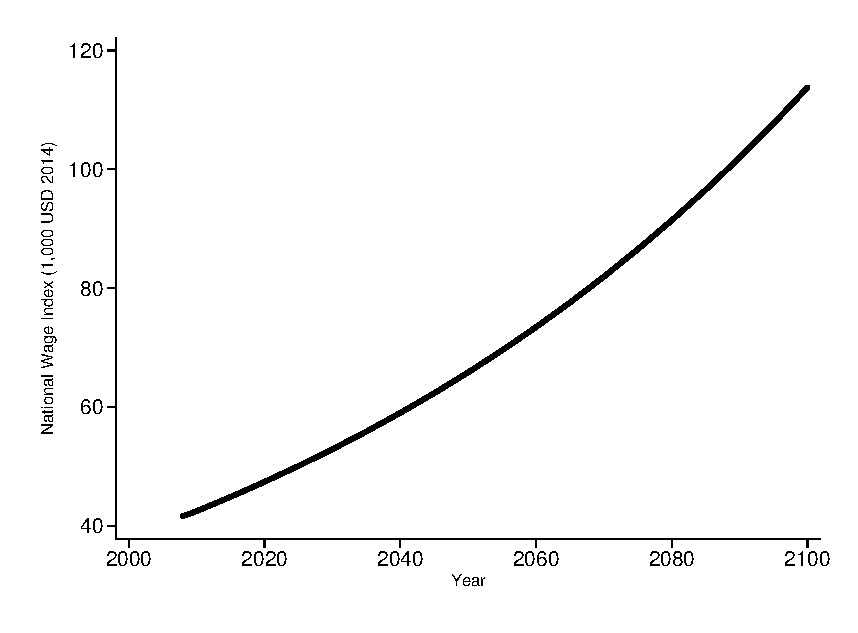
\includegraphics[height=3.5in]{AppOutput/Health/nwi.eps}
%\floatfoot{
%\footnotesize
%\noindent Note: Real wage growth projections are taken from Table VI.F6 in the 2009 Social Security Trustees Report \citep{Trustees_2009_Annual-Report-Old-Age-Survivors}. In years after the Trustees report projections, real wage growth is assumed to be 1.1\% annually.
%}
%\end{figure}

\noindent The real medical cost growth factor in each year is calculated by first finding the minimum of (i) the year-over-year GDP growth plus year-over-year excess medical cost growth or (ii) the Affordable Care Act cap on year-over-year medical cost growth. In order to obtain the medical cost adjustment factor for the current year of the simulation, FAM takes the cumulative product of the yearly growth factors since 2004 and then divides it by the relative growth in the labor force since 2004.\footnote{The medical cost growth assumptions come from Congressional Budget Office and SSA assumptions.
The year-over-year growth assumptions for medical costs are shown in Figure \ref{figure:medgrowth_yearly}.
The 2010-2019 GDP assumptions are based on CBO's analysis of the President's Budget, March 2009.
GDP assumptions for 2020-2100 are based on the 2008 OASDI Trustee's Report long-term projection of 2.1\% real GDP growth.} \\


\begin{figure}
\caption{Year-over-Year Excess Real Growth in Medical Costs} \label{figure:medgrowth_yearly}
 \centering
	 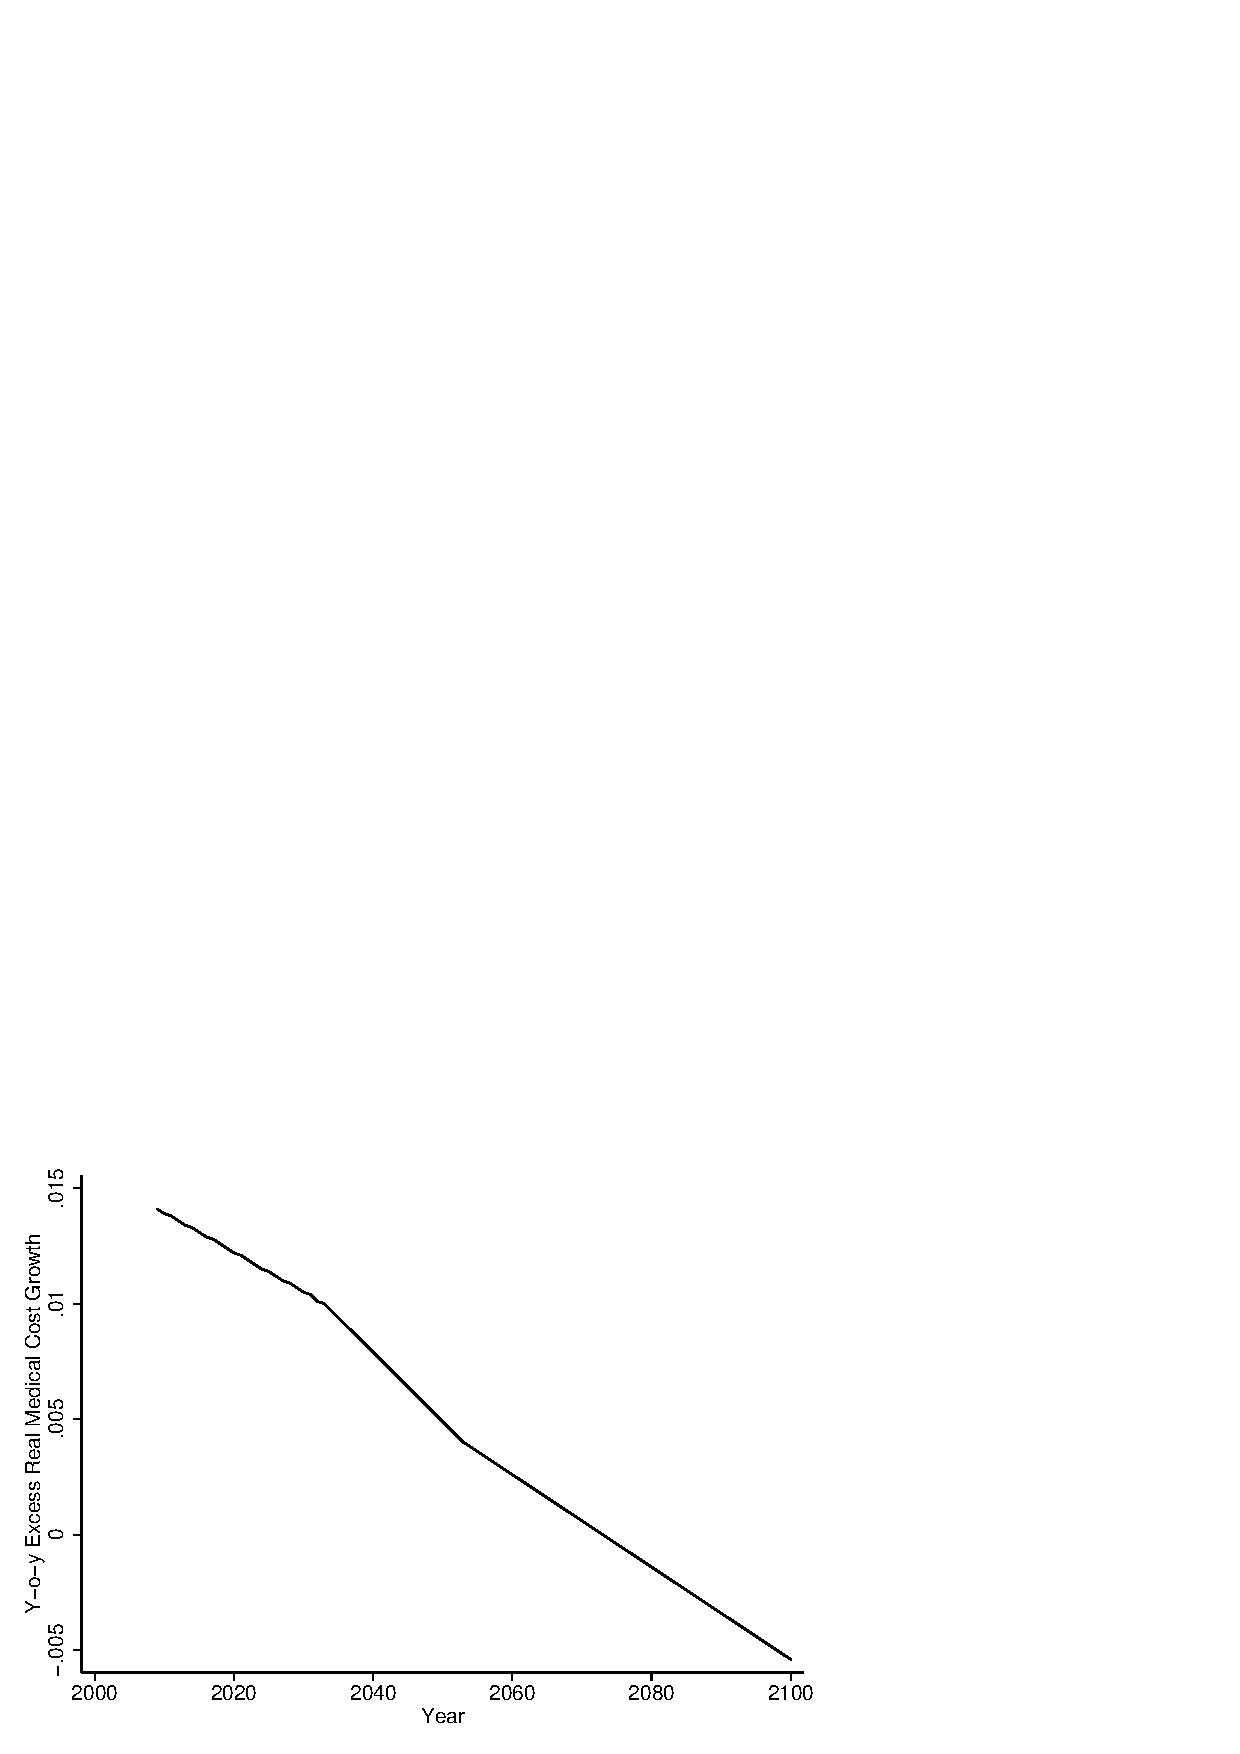
\includegraphics[height=3.5in]{AppOutput/Health/medgrowth_yearly}
\floatfoot{
\footnotesize
\noindent Sources: Congressional Budget Office, Social Security Administration.\\
\noindent Note: The year-over-year excess real medical cost growth over GDP is used to model medical cost growth in FAM.
}
\end{figure}

\subsubsection{Bootstrap Sampling Strategy}

\noindent The data sets used for estimating models in FAM are resampled in order to get estimates of sampling error in simulated outcomes.  PSID, HRS, MEPS, and MCBS all have complex survey designs that incorporate stratification and clustering.  In each of these data sets, the exact sampling strata and clusters are not publicly available, but approximations are included for the purpose of variance estimation.  The bootstrap methods in FAM were developed to implement the sampling strategy of \citet{McCarthy-Snowden_1985_Bootstrap}: randomly select $n_h-1$ sampling units with replacement from stratum $h$, where $n_h$ is the number of sampling units in stratum $h$. \\

\noindent PSID started with an initial sample of families in 1968.  Each generation of children from those families became sample members as they formed their own households.  The sample members present in the 1999--2013 PSID waves are used to estimate FAM models.   The PSID data used for estimation also includes a sample targeting immigrants that entered in 1997.  We randomly select one cluster from each variance estimation stratum in the 1968 and 1997 cohorts, with replacement.  Any family (original sample members or their descendants) belonging to that cluster are eligible to be included in the estimation for that bootstrap sample. \\

\noindent The HRS is resampled at the household level. From each variance estimation stratum, $n_h-1$ households are randomly selected with replacement, where $n_h$ is the number of households in the stratum. Observations for each household member are eligible to be included in the estimation for that bootstrap sample. \\

\noindent In MCBS, $n_h-1$ individuals are resampled with replacement from each variance estimation stratum, where $n_h$ is the number of individual beneficiaries in the stratum. \\

\noindent MEPS is resampled by dwelling unit.  Each MEPS bootstrap sample randomly selects $n_h-1$ dwelling units with replacement from each variance estimation stratum, where $n_h$ is the number of dwelling units in the stratum.  All members of the dwelling unit are eligible to be in the estimation sample.

\subsubsection{Medical Costs Before Age 30 Interview}

\noindent Data on utilization of medical services is sparse before the age 30 interview.  There are questions about utilization in the age 12, 15, and 21 interviews along with records of births for female subjects.  We combined this with information about demographics, family structure, and parents' utilization of public services to estimate medical costs at each age from 8 to 32.  Models were estimated separately for males and females.  All imputation and cost models are estimated using MEPS data. \\

\noindent Medical costs for ages 8 to 11 were estimated in three stages using age 12 interview data. First, we impute whether or not a subject spent a week in the hospital for those subjects who are missing this information in their age 12 interview.  The imputation model predicts utilization based on race and whether or not the subject was ever diagnosed with asthma between ages 8--11.  Next we separate the ABC and CARE subjects into the group that spent a week in the hospital in this age range and the group that did not.  For the group that did not spend any time in the hospital, we predicted medical costs as a two stage model.  The first stage predicts whether there were any medical costs at all.  Then, the second stage predicts the amount of medical costs for those subjects who were predicted to have some costs.  We assume the group that spent time in the hospital had some medical costs, so we skip the first stage and go directly to predicting the amount.  The cost models use race, asthma diagnosis, whether or not the father was absent from the home, family use of food stamps, and number of siblings as predictors.\\

\noindent Medical costs for ages 12 to 14 follow a strategy similar to the age 8--11 costs. First, we impute whether or not a subject had any hospitalization for those subjects who do not report this in their age 15 interview.  Imputations are based on race and presence or a	bsence of an asthma diagnosis between ages 12--14.  Again, we separated the ABC and CARE subjects into a group that had a hospitalization between age 8--11 and a group that did not.  A two-stage model was used to predict medical costs for those with no hospitalization.  Medical costs for the group that had a hospitalization were estimated directly from a single-stage model.  These cost models use race, asthma diagnosis, whether the mother, father, or both parents were absent from the home, family use of food stamps, and number of siblings.\\

\noindent To estimate medical costs for ages 15 to 20, we first impute whether or not the subject spent time in the hospital for those who are missing this information in the age 21 interview.  The imputation model was based on race, asthma diagnosis between ages 15--20, and, for females, the birth of any children.  The age 21 interview asks about the number of days spent in the hospital.  However, it does not record the ages at which these hospital stays occurred.  Considering the difficulty of assigning the hospital days to specific ages in the absence of other information, we decided to use only the indicator of whether or not there were any days spent in the hospital.  Next, we separated subjects into a group that spent some time in the hospital between ages 15--20 and those who did not.  As before, we used the direct model to predict costs for those who had been to the hospital and used a two-stage model for those who had not.  The cost models predict costs based on race, asthma diagnosis, any births (female model only), use of food stamps, whether or not the subject was working age, work status, living at college, and living with parents, and marital status.\\

\noindent Unlike the interviews at younger ages, the age 30 interview does not ask about utilization of medical services.  To estimate costs for ages 21--31, we skipped the utilization imputation step and moved directly to cost models. We used two-stage cost models.  The first stage predicts whether or not there were any costs based on race, asthma diagnosis between ages 21-31, education, use of food stamps, any births (female model only), whether or not the subject was working age, living at college, living with parents, and marital status.

\setcounter{figure}{0}  \renewcommand{\thefigure}{O.\arabic{figure}}
\setcounter{table}{0}   \renewcommand{\thetable}{O.\arabic{table}}
\section{{Expanding the Analyzed Outcomes}} \label{appendix:moreoutcomes}

\noindent In this appendix, we expand the analysis in Section~\ref{section:results} by considering an additional set of outcomes. Instead of considering \noutcomes, we consider \noutcomesexpp\ when pooling the sample and \noutcomesexpm\ and \noutcomesexpf\ when for males and females, respectively.\footnote{We fail to estimate some treatment effects because in some cases the treatment indicator and the controls entirely determine the outcome. For the \noutcomes\ in Section~\ref{section:results}, we do not have this problem.} The difference between this set of outcomes and the set we present in Section~\ref{section:results} is that (i) the outcomes in Section~\ref{section:results} contain outcomes we monetize when computing the cost-benefit analysis; and (ii) it is not entirely clear if treatment should have an effect on the outcomes we add in this appendix. The \noutcomes\ outcomes in this appendix include the \noutcomes\ outcomes in Section~\ref{section:results}.\\

\noindent To illustrate the difference between the outcomes in this appendix and the outcomes in Section~\ref{section:results}, consider two outcomes related to employment. In Section~\ref{section:results}, we include employment at age 30. In this appendix, we include both employment at age 30 and job satisfaction at age 30. Job satisfaction is a subjective variable, and it is not as clear what the effect of treatment on outcome is.\\

\noindent Table~\ref{table:abccare_rslt_pooled_counts_all} presents the results for the pooled sample, and Table~\ref{table:abccare_rslt_male_counts_all} and \ref{table:abccare_rslt_female_counts_all} present the results for males and females. It is still the case both that (i) we find a majority of positive treatment effects; and (ii) more than 10\% of these positive treatment effects are significant at the 10\%. It is true that the results weaken if compared to those we consider in Section~\ref{section:results}, but this is expected given how we construct the lists of outcomes. Appendix~\ref{appendix:morebycat} present the results by categories. We present the detailed point estimates in an additional appendix, for brevity.

	\begin{table}[H]
     \caption{Combining Functions, Pooled Sample} 
     \label{table:abccare_rslt_pooled_counts_all}
	
  \begin{tabular}{ccccccccc}
  \toprule
     & \scriptsize{(1)} & \scriptsize{(2)} & \scriptsize{(3)} & \scriptsize{(4)} & \scriptsize{(5)} & \scriptsize{(6)} & \scriptsize{(7)} & \scriptsize{(8)} \\ 
    \midrule

    \mc{1}{l}{\scriptsize{\% Pos. TE}} & \mc{1}{c}{\scriptsize{60}} & \mc{1}{c}{\scriptsize{62}} & \mc{1}{c}{\scriptsize{60}} & \mc{1}{c}{\scriptsize{65}} & \mc{1}{c}{\scriptsize{63}} & \mc{1}{c}{\scriptsize{59}} & \mc{1}{c}{\scriptsize{59}} & \mc{1}{c}{\scriptsize{61}} \\  

     & \mc{1}{c}{\scriptsize{\textbf{(0.013)}}} & \mc{1}{c}{\scriptsize{\textbf{(0.000)}}} & \mc{1}{c}{\scriptsize{\textbf{(0.013)}}} & \mc{1}{c}{\scriptsize{\textbf{(0.000)}}} & \mc{1}{c}{\scriptsize{\textbf{(0.000)}}} & \mc{1}{c}{\scriptsize{\textbf{(0.013)}}} & \mc{1}{c}{\scriptsize{\textbf{(0.013)}}} & \mc{1}{c}{\scriptsize{\textbf{(0.013)}}} \\  

    \mc{1}{l}{\scriptsize{\% Pos. TE $|$ 10\% Significance}} & \mc{1}{c}{\scriptsize{28}} & \mc{1}{c}{\scriptsize{23}} & \mc{1}{c}{\scriptsize{19}} & \mc{1}{c}{\scriptsize{16}} & \mc{1}{c}{\scriptsize{21}} & \mc{1}{c}{\scriptsize{24}} & \mc{1}{c}{\scriptsize{21}} & \mc{1}{c}{\scriptsize{27}} \\  

     & \mc{1}{c}{\scriptsize{\textbf{(0.000)}}} & \mc{1}{c}{\scriptsize{\textbf{(0.000)}}} & \mc{1}{c}{\scriptsize{\textbf{(0.026)}}} & \mc{1}{c}{\scriptsize{\textbf{(0.092)}}} & \mc{1}{c}{\scriptsize{\textbf{(0.026)}}} & \mc{1}{c}{\scriptsize{\textbf{(0.000)}}} & \mc{1}{c}{\scriptsize{\textbf{(0.000)}}} & \mc{1}{c}{\scriptsize{\textbf{(0.000)}}} \\  

  \bottomrule
  \end{tabular}

	\end{table}  

	\begin{table}[H]
     \caption{Combining Functions, Male Sample} 
     \label{table:abccare_rslt_male_counts_all}
	
  \begin{tabular}{ccccccccc}
  \toprule
     & \scriptsize{(1)} & \scriptsize{(2)} & \scriptsize{(3)} & \scriptsize{(4)} & \scriptsize{(5)} & \scriptsize{(6)} & \scriptsize{(7)} & \scriptsize{(8)} \\ 
    \midrule

    \mc{1}{l}{\scriptsize{\% Pos. TE}} & \mc{1}{c}{\scriptsize{52}} & \mc{1}{c}{\scriptsize{54}} & \mc{1}{c}{\scriptsize{39}} & \mc{1}{c}{\scriptsize{46}} & \mc{1}{c}{\scriptsize{40}} & \mc{1}{c}{\scriptsize{55}} & \mc{1}{c}{\scriptsize{57}} & \mc{1}{c}{\scriptsize{56}} \\  

     & \mc{1}{c}{\scriptsize{(0.289)}} & \mc{1}{c}{\scriptsize{(0.184)}} & \mc{1}{c}{\scriptsize{(0.987)}} & \mc{1}{c}{\scriptsize{(0.671)}} & \mc{1}{c}{\scriptsize{(0.961)}} & \mc{1}{c}{\scriptsize{(0.158)}} & \mc{1}{c}{\scriptsize{\textbf{(0.079)}}} & \mc{1}{c}{\scriptsize{(0.171)}} \\  

    \mc{1}{l}{\scriptsize{\% Pos. TE $|$ 10\% Significance}} & \mc{1}{c}{\scriptsize{15}} & \mc{1}{c}{\scriptsize{16}} & \mc{1}{c}{\scriptsize{9}} & \mc{1}{c}{\scriptsize{8}} & \mc{1}{c}{\scriptsize{8}} & \mc{1}{c}{\scriptsize{17}} & \mc{1}{c}{\scriptsize{14}} & \mc{1}{c}{\scriptsize{16}} \\  

     & \mc{1}{c}{\scriptsize{(0.132)}} & \mc{1}{c}{\scriptsize{\textbf{(0.053)}}} & \mc{1}{c}{\scriptsize{(0.539)}} & \mc{1}{c}{\scriptsize{(0.618)}} & \mc{1}{c}{\scriptsize{(0.724)}} & \mc{1}{c}{\scriptsize{\textbf{(0.026)}}} & \mc{1}{c}{\scriptsize{(0.118)}} & \mc{1}{c}{\scriptsize{\textbf{(0.053)}}} \\  

  \bottomrule
  \end{tabular}
	\end{table}  

	\begin{table}[H]
     \caption{Combining Functions, Female Sample} 
     \label{table:abccare_rslt_female_counts_all}
	
  \begin{tabular}{ccccccccc}
  \toprule
     & \scriptsize{(1)} & \scriptsize{(2)} & \scriptsize{(3)} & \scriptsize{(4)} & \scriptsize{(5)} & \scriptsize{(6)} & \scriptsize{(7)} & \scriptsize{(8)} \\ 
    \midrule

     & \scriptsize{(1)} & \scriptsize{(2)} & \scriptsize{(3)} & \scriptsize{(4)} & \scriptsize{(5)} & \scriptsize{(6)} & \scriptsize{(7)} & \scriptsize{(8)} \\ 
    \hline  

    \mc{1}{l}{\scriptsize{\% Pos. TE}} & \mc{1}{c}{\scriptsize{67}} & \mc{1}{c}{\scriptsize{68}} & \mc{1}{c}{\scriptsize{70}} & \mc{1}{c}{\scriptsize{72}} & \mc{1}{c}{\scriptsize{71}} & \mc{1}{c}{\scriptsize{62}} & \mc{1}{c}{\scriptsize{61}} & \mc{1}{c}{\scriptsize{63}} \\  

     & \mc{1}{c}{\scriptsize{\textbf{(0.000)}}} & \mc{1}{c}{\scriptsize{\textbf{(0.000)}}} & \mc{1}{c}{\scriptsize{\textbf{(0.000)}}} & \mc{1}{c}{\scriptsize{\textbf{(0.000)}}} & \mc{1}{c}{\scriptsize{\textbf{(0.000)}}} & \mc{1}{c}{\scriptsize{\textbf{(0.013)}}} & \mc{1}{c}{\scriptsize{\textbf{(0.000)}}} & \mc{1}{c}{\scriptsize{\textbf{(0.000)}}} \\  

    \mc{1}{l}{\scriptsize{\% Pos. TE $|$ 10\% Significance}} & \mc{1}{c}{\scriptsize{31}} & \mc{1}{c}{\scriptsize{25}} & \mc{1}{c}{\scriptsize{31}} & \mc{1}{c}{\scriptsize{25}} & \mc{1}{c}{\scriptsize{33}} & \mc{1}{c}{\scriptsize{23}} & \mc{1}{c}{\scriptsize{18}} & \mc{1}{c}{\scriptsize{26}} \\  

     & \mc{1}{c}{\scriptsize{\textbf{(0.000)}}} & \mc{1}{c}{\scriptsize{\textbf{(0.000)}}} & \mc{1}{c}{\scriptsize{\textbf{(0.000)}}} & \mc{1}{c}{\scriptsize{\textbf{(0.000)}}} & \mc{1}{c}{\scriptsize{\textbf{(0.000)}}} & \mc{1}{c}{\scriptsize{\textbf{(0.000)}}} & \mc{1}{c}{\scriptsize{\textbf{(0.053)}}} & \mc{1}{c}{\scriptsize{\textbf{(0.000)}}} \\  

  \bottomrule
  \end{tabular}
	\end{table}  

\subsection{{Outcomes by Category}} \label{appendix:morebycat}


	\begin{sidewaystable}[H]
     \caption{Combining Functions by Category, Pooled Sample} 
     \label{table:abccare_rslt_pooled_counts_n50a100_all}
	  \begin{tabular}{cccccccccc}
  \toprule

    \scriptsize{Category} & \scriptsize{(1)} & \scriptsize{(2)} & \scriptsize{(3)} & \scriptsize{(4)} & \scriptsize{(5)} & \scriptsize{(6)} & \scriptsize{(7)} & \scriptsize{(8)} &  \\ 
    \midrule  

    \mc{1}{l}{\scriptsize{Cognitive Skills}} & \mc{1}{c}{\scriptsize{100}} & \mc{1}{c}{\scriptsize{96}} & \mc{1}{c}{\scriptsize{100}} & \mc{1}{c}{\scriptsize{96}} & \mc{1}{c}{\scriptsize{100}} & \mc{1}{c}{\scriptsize{96}} & \mc{1}{c}{\scriptsize{96}} & \mc{1}{c}{\scriptsize{96}} & \mc{1}{c}{\scriptsize{25}} \\  

     & \mc{1}{c}{\scriptsize{\textbf{(0.000)}}} & \mc{1}{c}{\scriptsize{\textbf{(0.000)}}} & \mc{1}{c}{\scriptsize{\textbf{(0.000)}}} & \mc{1}{c}{\scriptsize{\textbf{(0.000)}}} & \mc{1}{c}{\scriptsize{\textbf{(0.000)}}} & \mc{1}{c}{\scriptsize{\textbf{(0.000)}}} & \mc{1}{c}{\scriptsize{\textbf{(0.000)}}} & \mc{1}{c}{\scriptsize{\textbf{(0.000)}}} &  \\  

    \mc{1}{l}{\scriptsize{Noncognitive Skills}} & \mc{1}{c}{\scriptsize{49}} & \mc{1}{c}{\scriptsize{54}} & \mc{1}{c}{\scriptsize{49}} & \mc{1}{c}{\scriptsize{58}} & \mc{1}{c}{\scriptsize{60}} & \mc{1}{c}{\scriptsize{50}} & \mc{1}{c}{\scriptsize{52}} & \mc{1}{c}{\scriptsize{54}} & \mc{1}{c}{\scriptsize{117}} \\  

     & \mc{1}{c}{\scriptsize{(0.539)}} & \mc{1}{c}{\scriptsize{(0.316)}} & \mc{1}{c}{\scriptsize{(0.513)}} & \mc{1}{c}{\scriptsize{(0.184)}} & \mc{1}{c}{\scriptsize{(0.145)}} & \mc{1}{c}{\scriptsize{(0.461)}} & \mc{1}{c}{\scriptsize{(0.395)}} & \mc{1}{c}{\scriptsize{(0.329)}} &  \\  

    \mc{1}{l}{\scriptsize{Mother's Employment, Education, and Income}} & \mc{1}{c}{\scriptsize{50}} & \mc{1}{c}{\scriptsize{50}} & \mc{1}{c}{\scriptsize{25}} & \mc{1}{c}{\scriptsize{75}} & \mc{1}{c}{\scriptsize{50}} & \mc{1}{c}{\scriptsize{50}} & \mc{1}{c}{\scriptsize{50}} & \mc{1}{c}{\scriptsize{25}} & \mc{1}{c}{\scriptsize{4}} \\  

     & \mc{1}{c}{\scriptsize{(0.671)}} & \mc{1}{c}{\scriptsize{(0.237)}} & \mc{1}{c}{\scriptsize{(0.987)}} & \mc{1}{c}{\scriptsize{\textbf{(0.039)}}} & \mc{1}{c}{\scriptsize{(0.671)}} & \mc{1}{c}{\scriptsize{(0.566)}} & \mc{1}{c}{\scriptsize{(0.263)}} & \mc{1}{c}{\scriptsize{(0.987)}} &  \\  

    \mc{1}{l}{\scriptsize{Childhood Household Environment}} & \mc{1}{c}{\scriptsize{67}} & \mc{1}{c}{\scriptsize{80}} & \mc{1}{c}{\scriptsize{53}} & \mc{1}{c}{\scriptsize{53}} & \mc{1}{c}{\scriptsize{60}} & \mc{1}{c}{\scriptsize{80}} & \mc{1}{c}{\scriptsize{60}} & \mc{1}{c}{\scriptsize{93}} & \mc{1}{c}{\scriptsize{15}} \\  

     & \mc{1}{c}{\scriptsize{(0.105)}} & \mc{1}{c}{\scriptsize{\textbf{(0.013)}}} & \mc{1}{c}{\scriptsize{(0.132)}} & \mc{1}{c}{\scriptsize{(0.474)}} & \mc{1}{c}{\scriptsize{\textbf{(0.079)}}} & \mc{1}{c}{\scriptsize{\textbf{(0.026)}}} & \mc{1}{c}{\scriptsize{(0.224)}} & \mc{1}{c}{\scriptsize{\textbf{(0.000)}}} &  \\  

    \mc{1}{l}{\scriptsize{Adult Household Environment}} & \mc{1}{c}{\scriptsize{78}} & \mc{1}{c}{\scriptsize{67}} & \mc{1}{c}{\scriptsize{56}} & \mc{1}{c}{\scriptsize{56}} & \mc{1}{c}{\scriptsize{44}} & \mc{1}{c}{\scriptsize{78}} & \mc{1}{c}{\scriptsize{67}} & \mc{1}{c}{\scriptsize{67}} & \mc{1}{c}{\scriptsize{9}} \\  

     & \mc{1}{c}{\scriptsize{\textbf{(0.000)}}} & \mc{1}{c}{\scriptsize{\textbf{(0.066)}}} & \mc{1}{c}{\scriptsize{(0.342)}} & \mc{1}{c}{\scriptsize{(0.368)}} & \mc{1}{c}{\scriptsize{(0.684)}} & \mc{1}{c}{\scriptsize{\textbf{(0.000)}}} & \mc{1}{c}{\scriptsize{\textbf{(0.026)}}} & \mc{1}{c}{\scriptsize{\textbf{(0.026)}}} &  \\  

    \mc{1}{l}{\scriptsize{Education, Employment, Income}} & \mc{1}{c}{\scriptsize{54}} & \mc{1}{c}{\scriptsize{54}} & \mc{1}{c}{\scriptsize{59}} & \mc{1}{c}{\scriptsize{71}} & \mc{1}{c}{\scriptsize{57}} & \mc{1}{c}{\scriptsize{54}} & \mc{1}{c}{\scriptsize{54}} & \mc{1}{c}{\scriptsize{61}} & \mc{1}{c}{\scriptsize{28}} \\  

     & \mc{1}{c}{\scriptsize{(0.395)}} & \mc{1}{c}{\scriptsize{(0.382)}} & \mc{1}{c}{\scriptsize{(0.263)}} & \mc{1}{c}{\scriptsize{\textbf{(0.066)}}} & \mc{1}{c}{\scriptsize{(0.368)}} & \mc{1}{c}{\scriptsize{(0.329)}} & \mc{1}{c}{\scriptsize{(0.342)}} & \mc{1}{c}{\scriptsize{(0.171)}} &  \\  

    \mc{1}{l}{\scriptsize{Crime}} & \mc{1}{c}{\scriptsize{33}} & \mc{1}{c}{\scriptsize{33}} & \mc{1}{c}{\scriptsize{67}} & \mc{1}{c}{\scriptsize{33}} & \mc{1}{c}{\scriptsize{33}} & \mc{1}{c}{\scriptsize{33}} & \mc{1}{c}{\scriptsize{33}} & \mc{1}{c}{\scriptsize{33}} & \mc{1}{c}{\scriptsize{3}} \\  

     & \mc{1}{c}{\scriptsize{(0.513)}} & \mc{1}{c}{\scriptsize{(0.868)}} & \mc{1}{c}{\scriptsize{(0.513)}} & \mc{1}{c}{\scriptsize{(0.882)}} & \mc{1}{c}{\scriptsize{(0.908)}} & \mc{1}{c}{\scriptsize{(0.461)}} & \mc{1}{c}{\scriptsize{(0.816)}} & \mc{1}{c}{\scriptsize{(0.842)}} &  \\  

    \mc{1}{l}{\scriptsize{Childhood Health}} & \mc{1}{c}{\scriptsize{71}} & \mc{1}{c}{\scriptsize{71}} & \mc{1}{c}{\scriptsize{57}} & \mc{1}{c}{\scriptsize{57}} & \mc{1}{c}{\scriptsize{57}} & \mc{1}{c}{\scriptsize{71}} & \mc{1}{c}{\scriptsize{64}} & \mc{1}{c}{\scriptsize{79}} & \mc{1}{c}{\scriptsize{14}} \\  

     & \mc{1}{c}{\scriptsize{\textbf{(0.013)}}} & \mc{1}{c}{\scriptsize{\textbf{(0.053)}}} & \mc{1}{c}{\scriptsize{(0.237)}} & \mc{1}{c}{\scriptsize{(0.237)}} & \mc{1}{c}{\scriptsize{(0.224)}} & \mc{1}{c}{\scriptsize{\textbf{(0.013)}}} & \mc{1}{c}{\scriptsize{\textbf{(0.053)}}} & \mc{1}{c}{\scriptsize{\textbf{(0.000)}}} &  \\  

    \mc{1}{l}{\scriptsize{Adult Health}} & \mc{1}{c}{\scriptsize{63}} & \mc{1}{c}{\scriptsize{60}} & \mc{1}{c}{\scriptsize{66}} & \mc{1}{c}{\scriptsize{61}} & \mc{1}{c}{\scriptsize{62}} & \mc{1}{c}{\scriptsize{54}} & \mc{1}{c}{\scriptsize{51}} & \mc{1}{c}{\scriptsize{51}} & \mc{1}{c}{\scriptsize{86}} \\  

     & \mc{1}{c}{\scriptsize{\textbf{(0.013)}}} & \mc{1}{c}{\scriptsize{\textbf{(0.013)}}} & \mc{1}{c}{\scriptsize{\textbf{(0.000)}}} & \mc{1}{c}{\scriptsize{\textbf{(0.013)}}} & \mc{1}{c}{\scriptsize{\textbf{(0.026)}}} & \mc{1}{c}{\scriptsize{(0.237)}} & \mc{1}{c}{\scriptsize{(0.447)}} & \mc{1}{c}{\scriptsize{(0.395)}} &  \\  

    \mc{1}{l}{\scriptsize{Mental Health}} & \mc{1}{c}{\scriptsize{64}} & \mc{1}{c}{\scriptsize{68}} & \mc{1}{c}{\scriptsize{62}} & \mc{1}{c}{\scriptsize{73}} & \mc{1}{c}{\scriptsize{64}} & \mc{1}{c}{\scriptsize{64}} & \mc{1}{c}{\scriptsize{75}} & \mc{1}{c}{\scriptsize{68}} & \mc{1}{c}{\scriptsize{56}} \\  

     & \mc{1}{c}{\scriptsize{(0.158)}} & \mc{1}{c}{\scriptsize{\textbf{(0.026)}}} & \mc{1}{c}{\scriptsize{(0.303)}} & \mc{1}{c}{\scriptsize{\textbf{(0.013)}}} & \mc{1}{c}{\scriptsize{(0.237)}} & \mc{1}{c}{\scriptsize{(0.105)}} & \mc{1}{c}{\scriptsize{\textbf{(0.000)}}} & \mc{1}{c}{\scriptsize{\textbf{(0.026)}}} &  \\  

  \bottomrule
  \end{tabular}

	\end{sidewaystable}   

	\begin{sidewaystable}[H]
     \caption{Combining Functions by Category $|$ 10\% Significance, Pooled Sample} 
     \label{table:abccare_rslt_pooled_counts_n10a10_all}
	  \begin{tabular}{cccccccccc}
  \toprule

    \scriptsize{Category} & \scriptsize{(1)} & \scriptsize{(2)} & \scriptsize{(3)} & \scriptsize{(4)} & \scriptsize{(5)} & \scriptsize{(6)} & \scriptsize{(7)} & \scriptsize{(8)} &  \\ 
    \midrule  

    \mc{1}{l}{\scriptsize{Cognitive Skills}} & \mc{1}{c}{\scriptsize{92}} & \mc{1}{c}{\scriptsize{88}} & \mc{1}{c}{\scriptsize{48}} & \mc{1}{c}{\scriptsize{48}} & \mc{1}{c}{\scriptsize{48}} & \mc{1}{c}{\scriptsize{88}} & \mc{1}{c}{\scriptsize{68}} & \mc{1}{c}{\scriptsize{88}} & \mc{1}{c}{\scriptsize{25}} \\  

     & \mc{1}{c}{\scriptsize{\textbf{(0.000)}}} & \mc{1}{c}{\scriptsize{\textbf{(0.000)}}} & \mc{1}{c}{\scriptsize{\textbf{(0.013)}}} & \mc{1}{c}{\scriptsize{\textbf{(0.000)}}} & \mc{1}{c}{\scriptsize{\textbf{(0.013)}}} & \mc{1}{c}{\scriptsize{\textbf{(0.000)}}} & \mc{1}{c}{\scriptsize{\textbf{(0.000)}}} & \mc{1}{c}{\scriptsize{\textbf{(0.000)}}} &  \\  

    \mc{1}{l}{\scriptsize{Noncognitive Skills}} & \mc{1}{c}{\scriptsize{20}} & \mc{1}{c}{\scriptsize{18}} & \mc{1}{c}{\scriptsize{11}} & \mc{1}{c}{\scriptsize{8}} & \mc{1}{c}{\scriptsize{11}} & \mc{1}{c}{\scriptsize{16}} & \mc{1}{c}{\scriptsize{15}} & \mc{1}{c}{\scriptsize{21}} & \mc{1}{c}{\scriptsize{117}} \\  

     & \mc{1}{c}{\scriptsize{\textbf{(0.053)}}} & \mc{1}{c}{\scriptsize{\textbf{(0.079)}}} & \mc{1}{c}{\scriptsize{(0.303)}} & \mc{1}{c}{\scriptsize{(0.618)}} & \mc{1}{c}{\scriptsize{(0.303)}} & \mc{1}{c}{\scriptsize{(0.105)}} & \mc{1}{c}{\scriptsize{(0.118)}} & \mc{1}{c}{\scriptsize{\textbf{(0.026)}}} &  \\  

    \mc{1}{l}{\scriptsize{Mother's Employment, Education, and Income}} & \mc{1}{c}{\scriptsize{0}} & \mc{1}{c}{\scriptsize{25}} & \mc{1}{c}{\scriptsize{25}} & \mc{1}{c}{\scriptsize{0}} & \mc{1}{c}{\scriptsize{25}} & \mc{1}{c}{\scriptsize{0}} & \mc{1}{c}{\scriptsize{25}} & \mc{1}{c}{\scriptsize{0}} & \mc{1}{c}{\scriptsize{4}} \\  

     & \mc{1}{c}{\scriptsize{(1.000)}} & \mc{1}{c}{\scriptsize{(0.368)}} & \mc{1}{c}{\scriptsize{\textbf{(0.079)}}} & \mc{1}{c}{\scriptsize{(0.395)}} & \mc{1}{c}{\scriptsize{\textbf{(0.053)}}} & \mc{1}{c}{\scriptsize{(1.000)}} & \mc{1}{c}{\scriptsize{\textbf{(0.039)}}} & \mc{1}{c}{\scriptsize{(0.461)}} &  \\  

    \mc{1}{l}{\scriptsize{Childhood Household Environment}} & \mc{1}{c}{\scriptsize{40}} & \mc{1}{c}{\scriptsize{7}} & \mc{1}{c}{\scriptsize{40}} & \mc{1}{c}{\scriptsize{27}} & \mc{1}{c}{\scriptsize{47}} & \mc{1}{c}{\scriptsize{27}} & \mc{1}{c}{\scriptsize{27}} & \mc{1}{c}{\scriptsize{40}} & \mc{1}{c}{\scriptsize{15}} \\  

     & \mc{1}{c}{\scriptsize{\textbf{(0.000)}}} & \mc{1}{c}{\scriptsize{(0.579)}} & \mc{1}{c}{\scriptsize{\textbf{(0.000)}}} & \mc{1}{c}{\scriptsize{\textbf{(0.039)}}} & \mc{1}{c}{\scriptsize{\textbf{(0.000)}}} & \mc{1}{c}{\scriptsize{\textbf{(0.092)}}} & \mc{1}{c}{\scriptsize{\textbf{(0.079)}}} & \mc{1}{c}{\scriptsize{\textbf{(0.053)}}} &  \\  

    \mc{1}{l}{\scriptsize{Adult Household Environment}} & \mc{1}{c}{\scriptsize{11}} & \mc{1}{c}{\scriptsize{22}} & \mc{1}{c}{\scriptsize{22}} & \mc{1}{c}{\scriptsize{11}} & \mc{1}{c}{\scriptsize{22}} & \mc{1}{c}{\scriptsize{11}} & \mc{1}{c}{\scriptsize{0}} & \mc{1}{c}{\scriptsize{0}} & \mc{1}{c}{\scriptsize{9}} \\  

     & \mc{1}{c}{\scriptsize{(0.434)}} & \mc{1}{c}{\scriptsize{\textbf{(0.039)}}} & \mc{1}{c}{\scriptsize{(0.211)}} & \mc{1}{c}{\scriptsize{(0.224)}} & \mc{1}{c}{\scriptsize{(0.197)}} & \mc{1}{c}{\scriptsize{(0.355)}} & \mc{1}{c}{\scriptsize{(1.000)}} & \mc{1}{c}{\scriptsize{(0.645)}} &  \\  

    \mc{1}{l}{\scriptsize{Education, Employment, Income}} & \mc{1}{c}{\scriptsize{21}} & \mc{1}{c}{\scriptsize{18}} & \mc{1}{c}{\scriptsize{22}} & \mc{1}{c}{\scriptsize{14}} & \mc{1}{c}{\scriptsize{29}} & \mc{1}{c}{\scriptsize{21}} & \mc{1}{c}{\scriptsize{14}} & \mc{1}{c}{\scriptsize{21}} & \mc{1}{c}{\scriptsize{28}} \\  

     & \mc{1}{c}{\scriptsize{\textbf{(0.026)}}} & \mc{1}{c}{\scriptsize{(0.145)}} & \mc{1}{c}{\scriptsize{\textbf{(0.079)}}} & \mc{1}{c}{\scriptsize{(0.132)}} & \mc{1}{c}{\scriptsize{\textbf{(0.079)}}} & \mc{1}{c}{\scriptsize{\textbf{(0.039)}}} & \mc{1}{c}{\scriptsize{(0.250)}} & \mc{1}{c}{\scriptsize{(0.132)}} &  \\  

    \mc{1}{l}{\scriptsize{Crime}} & \mc{1}{c}{\scriptsize{33}} & \mc{1}{c}{\scriptsize{0}} & \mc{1}{c}{\scriptsize{33}} & \mc{1}{c}{\scriptsize{0}} & \mc{1}{c}{\scriptsize{0}} & \mc{1}{c}{\scriptsize{0}} & \mc{1}{c}{\scriptsize{0}} & \mc{1}{c}{\scriptsize{0}} & \mc{1}{c}{\scriptsize{3}} \\  

     & \mc{1}{c}{\scriptsize{\textbf{(0.039)}}} & \mc{1}{c}{\scriptsize{(0.303)}} & \mc{1}{c}{\scriptsize{(0.250)}} & \mc{1}{c}{\scriptsize{(1.000)}} & \mc{1}{c}{\scriptsize{(1.000)}} & \mc{1}{c}{\scriptsize{(0.316)}} & \mc{1}{c}{\scriptsize{(1.000)}} & \mc{1}{c}{\scriptsize{(0.303)}} &  \\  

    \mc{1}{l}{\scriptsize{Childhood Health}} & \mc{1}{c}{\scriptsize{43}} & \mc{1}{c}{\scriptsize{36}} & \mc{1}{c}{\scriptsize{36}} & \mc{1}{c}{\scriptsize{21}} & \mc{1}{c}{\scriptsize{43}} & \mc{1}{c}{\scriptsize{36}} & \mc{1}{c}{\scriptsize{36}} & \mc{1}{c}{\scriptsize{36}} & \mc{1}{c}{\scriptsize{14}} \\  

     & \mc{1}{c}{\scriptsize{\textbf{(0.000)}}} & \mc{1}{c}{\scriptsize{\textbf{(0.013)}}} & \mc{1}{c}{\scriptsize{\textbf{(0.066)}}} & \mc{1}{c}{\scriptsize{(0.132)}} & \mc{1}{c}{\scriptsize{\textbf{(0.000)}}} & \mc{1}{c}{\scriptsize{\textbf{(0.000)}}} & \mc{1}{c}{\scriptsize{\textbf{(0.013)}}} & \mc{1}{c}{\scriptsize{\textbf{(0.000)}}} &  \\  

    \mc{1}{l}{\scriptsize{Adult Health}} & \mc{1}{c}{\scriptsize{23}} & \mc{1}{c}{\scriptsize{14}} & \mc{1}{c}{\scriptsize{15}} & \mc{1}{c}{\scriptsize{15}} & \mc{1}{c}{\scriptsize{18}} & \mc{1}{c}{\scriptsize{17}} & \mc{1}{c}{\scriptsize{13}} & \mc{1}{c}{\scriptsize{16}} & \mc{1}{c}{\scriptsize{86}} \\  

     & \mc{1}{c}{\scriptsize{\textbf{(0.000)}}} & \mc{1}{c}{\scriptsize{(0.211)}} & \mc{1}{c}{\scriptsize{(0.171)}} & \mc{1}{c}{\scriptsize{(0.118)}} & \mc{1}{c}{\scriptsize{\textbf{(0.066)}}} & \mc{1}{c}{\scriptsize{\textbf{(0.066)}}} & \mc{1}{c}{\scriptsize{(0.250)}} & \mc{1}{c}{\scriptsize{\textbf{(0.079)}}} &  \\  

    \mc{1}{l}{\scriptsize{Mental Health}} & \mc{1}{c}{\scriptsize{27}} & \mc{1}{c}{\scriptsize{27}} & \mc{1}{c}{\scriptsize{14}} & \mc{1}{c}{\scriptsize{20}} & \mc{1}{c}{\scriptsize{18}} & \mc{1}{c}{\scriptsize{25}} & \mc{1}{c}{\scriptsize{29}} & \mc{1}{c}{\scriptsize{34}} & \mc{1}{c}{\scriptsize{56}} \\  

     & \mc{1}{c}{\scriptsize{\textbf{(0.079)}}} & \mc{1}{c}{\scriptsize{(0.132)}} & \mc{1}{c}{\scriptsize{(0.289)}} & \mc{1}{c}{\scriptsize{(0.211)}} & \mc{1}{c}{\scriptsize{(0.224)}} & \mc{1}{c}{\scriptsize{(0.132)}} & \mc{1}{c}{\scriptsize{\textbf{(0.092)}}} & \mc{1}{c}{\scriptsize{\textbf{(0.000)}}} &  \\  

  \bottomrule
  \end{tabular}
	\end{sidewaystable}   

	\begin{sidewaystable}[H]
     \caption{Combining Functions by Category, Male Sample} 
     \label{table:abccare_rslt_male_counts_n50a100_all}
	  \begin{tabular}{cccccccccc}
  \toprule

    \scriptsize{Category} & \scriptsize{(1)} & \scriptsize{(2)} & \scriptsize{(3)} & \scriptsize{(4)} & \scriptsize{(5)} & \scriptsize{(6)} & \scriptsize{(7)} & \scriptsize{(8)} &  \\ 
    \midrule  

    \mc{1}{l}{\scriptsize{Cognitive Skills}} & \mc{1}{c}{\scriptsize{96}} & \mc{1}{c}{\scriptsize{84}} & \mc{1}{c}{\scriptsize{64}} & \mc{1}{c}{\scriptsize{60}} & \mc{1}{c}{\scriptsize{52}} & \mc{1}{c}{\scriptsize{96}} & \mc{1}{c}{\scriptsize{84}} & \mc{1}{c}{\scriptsize{84}} & \mc{1}{c}{\scriptsize{25}} \\  

     & \mc{1}{c}{\scriptsize{\textbf{(0.000)}}} & \mc{1}{c}{\scriptsize{\textbf{(0.000)}}} & \mc{1}{c}{\scriptsize{(0.303)}} & \mc{1}{c}{\scriptsize{(0.382)}} & \mc{1}{c}{\scriptsize{(0.474)}} & \mc{1}{c}{\scriptsize{\textbf{(0.000)}}} & \mc{1}{c}{\scriptsize{\textbf{(0.000)}}} & \mc{1}{c}{\scriptsize{\textbf{(0.000)}}} &  \\  

    \mc{1}{l}{\scriptsize{Noncognitive Skills}} & \mc{1}{c}{\scriptsize{42}} & \mc{1}{c}{\scriptsize{45}} & \mc{1}{c}{\scriptsize{28}} & \mc{1}{c}{\scriptsize{35}} & \mc{1}{c}{\scriptsize{34}} & \mc{1}{c}{\scriptsize{48}} & \mc{1}{c}{\scriptsize{50}} & \mc{1}{c}{\scriptsize{50}} & \mc{1}{c}{\scriptsize{117}} \\  

     & \mc{1}{c}{\scriptsize{(0.908)}} & \mc{1}{c}{\scriptsize{(0.645)}} & \mc{1}{c}{\scriptsize{(1.000)}} & \mc{1}{c}{\scriptsize{(0.934)}} & \mc{1}{c}{\scriptsize{(0.987)}} & \mc{1}{c}{\scriptsize{(0.579)}} & \mc{1}{c}{\scriptsize{(0.461)}} & \mc{1}{c}{\scriptsize{(0.539)}} &  \\  

    \mc{1}{l}{\scriptsize{Mother's Employment, Education, and Income}} & \mc{1}{c}{\scriptsize{50}} & \mc{1}{c}{\scriptsize{50}} & \mc{1}{c}{\scriptsize{50}} & \mc{1}{c}{\scriptsize{100}} & \mc{1}{c}{\scriptsize{50}} & \mc{1}{c}{\scriptsize{25}} & \mc{1}{c}{\scriptsize{50}} & \mc{1}{c}{\scriptsize{50}} & \mc{1}{c}{\scriptsize{4}} \\  

     & \mc{1}{c}{\scriptsize{(0.513)}} & \mc{1}{c}{\scriptsize{(0.658)}} & \mc{1}{c}{\scriptsize{(0.368)}} & \mc{1}{c}{\scriptsize{\textbf{(0.000)}}} & \mc{1}{c}{\scriptsize{(0.368)}} & \mc{1}{c}{\scriptsize{(0.961)}} & \mc{1}{c}{\scriptsize{(0.605)}} & \mc{1}{c}{\scriptsize{(0.632)}} &  \\  

    \mc{1}{l}{\scriptsize{Childhood Household Environment}} & \mc{1}{c}{\scriptsize{60}} & \mc{1}{c}{\scriptsize{87}} & \mc{1}{c}{\scriptsize{47}} & \mc{1}{c}{\scriptsize{53}} & \mc{1}{c}{\scriptsize{47}} & \mc{1}{c}{\scriptsize{71}} & \mc{1}{c}{\scriptsize{87}} & \mc{1}{c}{\scriptsize{80}} & \mc{1}{c}{\scriptsize{15}} \\  

     & \mc{1}{c}{\scriptsize{(0.329)}} & \mc{1}{c}{\scriptsize{\textbf{(0.000)}}} & \mc{1}{c}{\scriptsize{(0.605)}} & \mc{1}{c}{\scriptsize{(0.421)}} & \mc{1}{c}{\scriptsize{(0.579)}} & \mc{1}{c}{\scriptsize{(0.184)}} & \mc{1}{c}{\scriptsize{\textbf{(0.000)}}} & \mc{1}{c}{\scriptsize{\textbf{(0.039)}}} &  \\  

    \mc{1}{l}{\scriptsize{Adult Household Environment}} & \mc{1}{c}{\scriptsize{56}} & \mc{1}{c}{\scriptsize{44}} & \mc{1}{c}{\scriptsize{38}} & \mc{1}{c}{\scriptsize{33}} & \mc{1}{c}{\scriptsize{22}} & \mc{1}{c}{\scriptsize{56}} & \mc{1}{c}{\scriptsize{56}} & \mc{1}{c}{\scriptsize{44}} & \mc{1}{c}{\scriptsize{9}} \\  

     & \mc{1}{c}{\scriptsize{(0.395)}} & \mc{1}{c}{\scriptsize{(0.724)}} & \mc{1}{c}{\scriptsize{(0.618)}} & \mc{1}{c}{\scriptsize{(0.803)}} & \mc{1}{c}{\scriptsize{(1.000)}} & \mc{1}{c}{\scriptsize{(0.276)}} & \mc{1}{c}{\scriptsize{(0.237)}} & \mc{1}{c}{\scriptsize{(0.592)}} &  \\  

    \mc{1}{l}{\scriptsize{Education, Employment, Income}} & \mc{1}{c}{\scriptsize{32}} & \mc{1}{c}{\scriptsize{36}} & \mc{1}{c}{\scriptsize{32}} & \mc{1}{c}{\scriptsize{36}} & \mc{1}{c}{\scriptsize{36}} & \mc{1}{c}{\scriptsize{43}} & \mc{1}{c}{\scriptsize{32}} & \mc{1}{c}{\scriptsize{36}} & \mc{1}{c}{\scriptsize{28}} \\  

     & \mc{1}{c}{\scriptsize{(0.987)}} & \mc{1}{c}{\scriptsize{(0.934)}} & \mc{1}{c}{\scriptsize{(0.974)}} & \mc{1}{c}{\scriptsize{(0.934)}} & \mc{1}{c}{\scriptsize{(0.947)}} & \mc{1}{c}{\scriptsize{(0.750)}} & \mc{1}{c}{\scriptsize{(0.974)}} & \mc{1}{c}{\scriptsize{(0.947)}} &  \\  

    \mc{1}{l}{\scriptsize{Crime}} & \mc{1}{c}{\scriptsize{33}} & \mc{1}{c}{\scriptsize{33}} & \mc{1}{c}{\scriptsize{33}} & \mc{1}{c}{\scriptsize{0}} & \mc{1}{c}{\scriptsize{33}} & \mc{1}{c}{\scriptsize{33}} & \mc{1}{c}{\scriptsize{33}} & \mc{1}{c}{\scriptsize{33}} & \mc{1}{c}{\scriptsize{3}} \\  

     & \mc{1}{c}{\scriptsize{(0.882)}} & \mc{1}{c}{\scriptsize{(0.724)}} & \mc{1}{c}{\scriptsize{(0.513)}} & \mc{1}{c}{\scriptsize{(0.987)}} & \mc{1}{c}{\scriptsize{(0.987)}} & \mc{1}{c}{\scriptsize{(0.500)}} & \mc{1}{c}{\scriptsize{(0.789)}} & \mc{1}{c}{\scriptsize{(0.921)}} &  \\  

    \mc{1}{l}{\scriptsize{Childhood Health}} & \mc{1}{c}{\scriptsize{79}} & \mc{1}{c}{\scriptsize{79}} & \mc{1}{c}{\scriptsize{77}} & \mc{1}{c}{\scriptsize{69}} & \mc{1}{c}{\scriptsize{77}} & \mc{1}{c}{\scriptsize{86}} & \mc{1}{c}{\scriptsize{79}} & \mc{1}{c}{\scriptsize{86}} & \mc{1}{c}{\scriptsize{14}} \\  

     & \mc{1}{c}{\scriptsize{\textbf{(0.000)}}} & \mc{1}{c}{\scriptsize{\textbf{(0.039)}}} & \mc{1}{c}{\scriptsize{\textbf{(0.000)}}} & \mc{1}{c}{\scriptsize{(0.132)}} & \mc{1}{c}{\scriptsize{\textbf{(0.000)}}} & \mc{1}{c}{\scriptsize{\textbf{(0.000)}}} & \mc{1}{c}{\scriptsize{\textbf{(0.026)}}} & \mc{1}{c}{\scriptsize{\textbf{(0.000)}}} &  \\  

    \mc{1}{l}{\scriptsize{Adult Health}} & \mc{1}{c}{\scriptsize{68}} & \mc{1}{c}{\scriptsize{62}} & \mc{1}{c}{\scriptsize{58}} & \mc{1}{c}{\scriptsize{62}} & \mc{1}{c}{\scriptsize{58}} & \mc{1}{c}{\scriptsize{59}} & \mc{1}{c}{\scriptsize{62}} & \mc{1}{c}{\scriptsize{59}} & \mc{1}{c}{\scriptsize{74}} \\  

     & \mc{1}{c}{\scriptsize{\textbf{(0.000)}}} & \mc{1}{c}{\scriptsize{\textbf{(0.013)}}} & \mc{1}{c}{\scriptsize{(0.237)}} & \mc{1}{c}{\scriptsize{\textbf{(0.066)}}} & \mc{1}{c}{\scriptsize{(0.237)}} & \mc{1}{c}{\scriptsize{\textbf{(0.039)}}} & \mc{1}{c}{\scriptsize{\textbf{(0.000)}}} & \mc{1}{c}{\scriptsize{\textbf{(0.039)}}} &  \\  

    \mc{1}{l}{\scriptsize{Mental Health}} & \mc{1}{c}{\scriptsize{41}} & \mc{1}{c}{\scriptsize{52}} & \mc{1}{c}{\scriptsize{17}} & \mc{1}{c}{\scriptsize{37}} & \mc{1}{c}{\scriptsize{22}} & \mc{1}{c}{\scriptsize{46}} & \mc{1}{c}{\scriptsize{56}} & \mc{1}{c}{\scriptsize{52}} & \mc{1}{c}{\scriptsize{54}} \\  

     & \mc{1}{c}{\scriptsize{(0.750)}} & \mc{1}{c}{\scriptsize{(0.487)}} & \mc{1}{c}{\scriptsize{(1.000)}} & \mc{1}{c}{\scriptsize{(0.789)}} & \mc{1}{c}{\scriptsize{(1.000)}} & \mc{1}{c}{\scriptsize{(0.645)}} & \mc{1}{c}{\scriptsize{(0.408)}} & \mc{1}{c}{\scriptsize{(0.553)}} &  \\  

  \bottomrule
  \end{tabular}
	\end{sidewaystable}   

	\begin{sidewaystable}[H]
     \caption{Combining Functions by Category $|$ 10\% Significance, Male Sample} 
     \label{table:abccare_rslt_male_counts_n10a10_all}
	  \begin{tabular}{cccccccccc}
  \toprule

    \scriptsize{Category} & \scriptsize{(1)} & \scriptsize{(2)} & \scriptsize{(3)} & \scriptsize{(4)} & \scriptsize{(5)} & \scriptsize{(6)} & \scriptsize{(7)} & \scriptsize{(8)} &  \\ 
    \midrule  

    \mc{1}{l}{\scriptsize{Cognitive Skills}} & \mc{1}{c}{\scriptsize{48}} & \mc{1}{c}{\scriptsize{48}} & \mc{1}{c}{\scriptsize{24}} & \mc{1}{c}{\scriptsize{24}} & \mc{1}{c}{\scriptsize{24}} & \mc{1}{c}{\scriptsize{60}} & \mc{1}{c}{\scriptsize{44}} & \mc{1}{c}{\scriptsize{56}} & \mc{1}{c}{\scriptsize{25}} \\  

     & \mc{1}{c}{\scriptsize{\textbf{(0.039)}}} & \mc{1}{c}{\scriptsize{\textbf{(0.013)}}} & \mc{1}{c}{\scriptsize{(0.237)}} & \mc{1}{c}{\scriptsize{(0.158)}} & \mc{1}{c}{\scriptsize{(0.197)}} & \mc{1}{c}{\scriptsize{\textbf{(0.000)}}} & \mc{1}{c}{\scriptsize{\textbf{(0.000)}}} & \mc{1}{c}{\scriptsize{\textbf{(0.000)}}} &  \\  

    \mc{1}{l}{\scriptsize{Noncognitive Skills}} & \mc{1}{c}{\scriptsize{9}} & \mc{1}{c}{\scriptsize{8}} & \mc{1}{c}{\scriptsize{5}} & \mc{1}{c}{\scriptsize{4}} & \mc{1}{c}{\scriptsize{5}} & \mc{1}{c}{\scriptsize{10}} & \mc{1}{c}{\scriptsize{9}} & \mc{1}{c}{\scriptsize{12}} & \mc{1}{c}{\scriptsize{117}} \\  

     & \mc{1}{c}{\scriptsize{(0.487)}} & \mc{1}{c}{\scriptsize{(0.684)}} & \mc{1}{c}{\scriptsize{(0.908)}} & \mc{1}{c}{\scriptsize{(0.987)}} & \mc{1}{c}{\scriptsize{(0.895)}} & \mc{1}{c}{\scriptsize{(0.342)}} & \mc{1}{c}{\scriptsize{(0.447)}} & \mc{1}{c}{\scriptsize{(0.316)}} &  \\  

    \mc{1}{l}{\scriptsize{Mother's Employment, Education, and Income}} & \mc{1}{c}{\scriptsize{0}} & \mc{1}{c}{\scriptsize{0}} & \mc{1}{c}{\scriptsize{25}} & \mc{1}{c}{\scriptsize{25}} & \mc{1}{c}{\scriptsize{25}} & \mc{1}{c}{\scriptsize{0}} & \mc{1}{c}{\scriptsize{0}} & \mc{1}{c}{\scriptsize{0}} & \mc{1}{c}{\scriptsize{4}} \\  

     & \mc{1}{c}{\scriptsize{(0.987)}} & \mc{1}{c}{\scriptsize{(0.987)}} & \mc{1}{c}{\scriptsize{(0.250)}} & \mc{1}{c}{\scriptsize{(0.237)}} & \mc{1}{c}{\scriptsize{(0.237)}} & \mc{1}{c}{\scriptsize{(0.974)}} & \mc{1}{c}{\scriptsize{(0.974)}} & \mc{1}{c}{\scriptsize{(0.974)}} &  \\  

    \mc{1}{l}{\scriptsize{Childhood Household Environment}} & \mc{1}{c}{\scriptsize{7}} & \mc{1}{c}{\scriptsize{13}} & \mc{1}{c}{\scriptsize{7}} & \mc{1}{c}{\scriptsize{13}} & \mc{1}{c}{\scriptsize{7}} & \mc{1}{c}{\scriptsize{14}} & \mc{1}{c}{\scriptsize{20}} & \mc{1}{c}{\scriptsize{27}} & \mc{1}{c}{\scriptsize{15}} \\  

     & \mc{1}{c}{\scriptsize{(0.658)}} & \mc{1}{c}{\scriptsize{(0.434)}} & \mc{1}{c}{\scriptsize{(0.697)}} & \mc{1}{c}{\scriptsize{(0.316)}} & \mc{1}{c}{\scriptsize{(0.618)}} & \mc{1}{c}{\scriptsize{(0.224)}} & \mc{1}{c}{\scriptsize{(0.250)}} & \mc{1}{c}{\scriptsize{(0.197)}} &  \\  

    \mc{1}{l}{\scriptsize{Adult Household Environment}} & \mc{1}{c}{\scriptsize{0}} & \mc{1}{c}{\scriptsize{0}} & \mc{1}{c}{\scriptsize{12}} & \mc{1}{c}{\scriptsize{0}} & \mc{1}{c}{\scriptsize{11}} & \mc{1}{c}{\scriptsize{0}} & \mc{1}{c}{\scriptsize{0}} & \mc{1}{c}{\scriptsize{0}} & \mc{1}{c}{\scriptsize{9}} \\  

     & \mc{1}{c}{\scriptsize{(1.000)}} & \mc{1}{c}{\scriptsize{(1.000)}} & \mc{1}{c}{\scriptsize{(0.197)}} & \mc{1}{c}{\scriptsize{(0.697)}} & \mc{1}{c}{\scriptsize{(0.408)}} & \mc{1}{c}{\scriptsize{(0.618)}} & \mc{1}{c}{\scriptsize{(1.000)}} & \mc{1}{c}{\scriptsize{(1.000)}} &  \\  

    \mc{1}{l}{\scriptsize{Education, Employment, Income}} & \mc{1}{c}{\scriptsize{11}} & \mc{1}{c}{\scriptsize{7}} & \mc{1}{c}{\scriptsize{0}} & \mc{1}{c}{\scriptsize{4}} & \mc{1}{c}{\scriptsize{0}} & \mc{1}{c}{\scriptsize{11}} & \mc{1}{c}{\scriptsize{4}} & \mc{1}{c}{\scriptsize{7}} & \mc{1}{c}{\scriptsize{28}} \\  

     & \mc{1}{c}{\scriptsize{(0.408)}} & \mc{1}{c}{\scriptsize{(0.632)}} & \mc{1}{c}{\scriptsize{(0.882)}} & \mc{1}{c}{\scriptsize{(1.000)}} & \mc{1}{c}{\scriptsize{(1.000)}} & \mc{1}{c}{\scriptsize{(0.421)}} & \mc{1}{c}{\scriptsize{(0.908)}} & \mc{1}{c}{\scriptsize{(0.592)}} &  \\  

    \mc{1}{l}{\scriptsize{Crime}} & \mc{1}{c}{\scriptsize{0}} & \mc{1}{c}{\scriptsize{0}} & \mc{1}{c}{\scriptsize{0}} & \mc{1}{c}{\scriptsize{0}} & \mc{1}{c}{\scriptsize{0}} & \mc{1}{c}{\scriptsize{0}} & \mc{1}{c}{\scriptsize{0}} & \mc{1}{c}{\scriptsize{0}} & \mc{1}{c}{\scriptsize{3}} \\  

     & \mc{1}{c}{\scriptsize{(1.000)}} & \mc{1}{c}{\scriptsize{(1.000)}} & \mc{1}{c}{\scriptsize{(0.987)}} & \mc{1}{c}{\scriptsize{(0.987)}} & \mc{1}{c}{\scriptsize{(0.987)}} & \mc{1}{c}{\scriptsize{(0.276)}} & \mc{1}{c}{\scriptsize{(1.000)}} & \mc{1}{c}{\scriptsize{(0.316)}} &  \\  

    \mc{1}{l}{\scriptsize{Childhood Health}} & \mc{1}{c}{\scriptsize{29}} & \mc{1}{c}{\scriptsize{29}} & \mc{1}{c}{\scriptsize{46}} & \mc{1}{c}{\scriptsize{31}} & \mc{1}{c}{\scriptsize{31}} & \mc{1}{c}{\scriptsize{21}} & \mc{1}{c}{\scriptsize{14}} & \mc{1}{c}{\scriptsize{21}} & \mc{1}{c}{\scriptsize{14}} \\  

     & \mc{1}{c}{\scriptsize{(0.184)}} & \mc{1}{c}{\scriptsize{(0.145)}} & \mc{1}{c}{\scriptsize{\textbf{(0.000)}}} & \mc{1}{c}{\scriptsize{\textbf{(0.066)}}} & \mc{1}{c}{\scriptsize{\textbf{(0.079)}}} & \mc{1}{c}{\scriptsize{(0.276)}} & \mc{1}{c}{\scriptsize{(0.276)}} & \mc{1}{c}{\scriptsize{(0.263)}} &  \\  

    \mc{1}{l}{\scriptsize{Adult Health}} & \mc{1}{c}{\scriptsize{27}} & \mc{1}{c}{\scriptsize{31}} & \mc{1}{c}{\scriptsize{12}} & \mc{1}{c}{\scriptsize{14}} & \mc{1}{c}{\scriptsize{10}} & \mc{1}{c}{\scriptsize{31}} & \mc{1}{c}{\scriptsize{27}} & \mc{1}{c}{\scriptsize{26}} & \mc{1}{c}{\scriptsize{74}} \\  

     & \mc{1}{c}{\scriptsize{\textbf{(0.000)}}} & \mc{1}{c}{\scriptsize{\textbf{(0.000)}}} & \mc{1}{c}{\scriptsize{(0.368)}} & \mc{1}{c}{\scriptsize{(0.224)}} & \mc{1}{c}{\scriptsize{(0.461)}} & \mc{1}{c}{\scriptsize{\textbf{(0.000)}}} & \mc{1}{c}{\scriptsize{\textbf{(0.000)}}} & \mc{1}{c}{\scriptsize{\textbf{(0.000)}}} &  \\  

    \mc{1}{l}{\scriptsize{Mental Health}} & \mc{1}{c}{\scriptsize{0}} & \mc{1}{c}{\scriptsize{7}} & \mc{1}{c}{\scriptsize{0}} & \mc{1}{c}{\scriptsize{0}} & \mc{1}{c}{\scriptsize{0}} & \mc{1}{c}{\scriptsize{2}} & \mc{1}{c}{\scriptsize{2}} & \mc{1}{c}{\scriptsize{2}} & \mc{1}{c}{\scriptsize{54}} \\  

     & \mc{1}{c}{\scriptsize{(1.000)}} & \mc{1}{c}{\scriptsize{(0.474)}} & \mc{1}{c}{\scriptsize{(1.000)}} & \mc{1}{c}{\scriptsize{(1.000)}} & \mc{1}{c}{\scriptsize{(1.000)}} & \mc{1}{c}{\scriptsize{(1.000)}} & \mc{1}{c}{\scriptsize{(1.000)}} & \mc{1}{c}{\scriptsize{(1.000)}} &  \\  

  \bottomrule
  \end{tabular}
	\end{sidewaystable}   

	\begin{sidewaystable}[H]
     \caption{Combining Functions by Category, Female Sample} 
     \label{table:abccare_rslt_female_counts_n50a100_all}
	  \begin{tabular}{cccccccccc}
  \toprule

    \scriptsize{Category} & \scriptsize{(1)} & \scriptsize{(2)} & \scriptsize{(3)} & \scriptsize{(4)} & \scriptsize{(5)} & \scriptsize{(6)} & \scriptsize{(7)} & \scriptsize{(8)} &  \\ 
    \midrule  

    \mc{1}{l}{\scriptsize{Cognitive Skills}} & \mc{1}{c}{\scriptsize{100}} & \mc{1}{c}{\scriptsize{96}} & \mc{1}{c}{\scriptsize{100}} & \mc{1}{c}{\scriptsize{100}} & \mc{1}{c}{\scriptsize{100}} & \mc{1}{c}{\scriptsize{100}} & \mc{1}{c}{\scriptsize{92}} & \mc{1}{c}{\scriptsize{100}} & \mc{1}{c}{\scriptsize{25}} \\  

     & \mc{1}{c}{\scriptsize{\textbf{(0.000)}}} & \mc{1}{c}{\scriptsize{\textbf{(0.000)}}} & \mc{1}{c}{\scriptsize{\textbf{(0.000)}}} & \mc{1}{c}{\scriptsize{\textbf{(0.000)}}} & \mc{1}{c}{\scriptsize{\textbf{(0.000)}}} & \mc{1}{c}{\scriptsize{\textbf{(0.000)}}} & \mc{1}{c}{\scriptsize{\textbf{(0.000)}}} & \mc{1}{c}{\scriptsize{\textbf{(0.000)}}} &  \\  

    \mc{1}{l}{\scriptsize{Noncognitive Skills}} & \mc{1}{c}{\scriptsize{70}} & \mc{1}{c}{\scriptsize{70}} & \mc{1}{c}{\scriptsize{74}} & \mc{1}{c}{\scriptsize{74}} & \mc{1}{c}{\scriptsize{77}} & \mc{1}{c}{\scriptsize{57}} & \mc{1}{c}{\scriptsize{61}} & \mc{1}{c}{\scriptsize{66}} & \mc{1}{c}{\scriptsize{117}} \\  

     & \mc{1}{c}{\scriptsize{\textbf{(0.000)}}} & \mc{1}{c}{\scriptsize{\textbf{(0.000)}}} & \mc{1}{c}{\scriptsize{\textbf{(0.000)}}} & \mc{1}{c}{\scriptsize{\textbf{(0.000)}}} & \mc{1}{c}{\scriptsize{\textbf{(0.000)}}} & \mc{1}{c}{\scriptsize{(0.237)}} & \mc{1}{c}{\scriptsize{(0.105)}} & \mc{1}{c}{\scriptsize{\textbf{(0.013)}}} &  \\  

    \mc{1}{l}{\scriptsize{Mother's Employment, Education, and Income}} & \mc{1}{c}{\scriptsize{50}} & \mc{1}{c}{\scriptsize{25}} & \mc{1}{c}{\scriptsize{50}} & \mc{1}{c}{\scriptsize{25}} & \mc{1}{c}{\scriptsize{50}} & \mc{1}{c}{\scriptsize{50}} & \mc{1}{c}{\scriptsize{25}} & \mc{1}{c}{\scriptsize{50}} & \mc{1}{c}{\scriptsize{4}} \\  

     & \mc{1}{c}{\scriptsize{(0.842)}} & \mc{1}{c}{\scriptsize{(0.974)}} & \mc{1}{c}{\scriptsize{(0.724)}} & \mc{1}{c}{\scriptsize{(0.750)}} & \mc{1}{c}{\scriptsize{(0.645)}} & \mc{1}{c}{\scriptsize{(0.224)}} & \mc{1}{c}{\scriptsize{(0.803)}} & \mc{1}{c}{\scriptsize{(0.250)}} &  \\  

    \mc{1}{l}{\scriptsize{Childhood Household Environment}} & \mc{1}{c}{\scriptsize{73}} & \mc{1}{c}{\scriptsize{80}} & \mc{1}{c}{\scriptsize{60}} & \mc{1}{c}{\scriptsize{67}} & \mc{1}{c}{\scriptsize{60}} & \mc{1}{c}{\scriptsize{64}} & \mc{1}{c}{\scriptsize{64}} & \mc{1}{c}{\scriptsize{79}} & \mc{1}{c}{\scriptsize{15}} \\  

     & \mc{1}{c}{\scriptsize{\textbf{(0.039)}}} & \mc{1}{c}{\scriptsize{\textbf{(0.026)}}} & \mc{1}{c}{\scriptsize{\textbf{(0.066)}}} & \mc{1}{c}{\scriptsize{\textbf{(0.053)}}} & \mc{1}{c}{\scriptsize{(0.132)}} & \mc{1}{c}{\scriptsize{(0.263)}} & \mc{1}{c}{\scriptsize{(0.145)}} & \mc{1}{c}{\scriptsize{\textbf{(0.053)}}} &  \\  

    \mc{1}{l}{\scriptsize{Adult Household Environment}} & \mc{1}{c}{\scriptsize{78}} & \mc{1}{c}{\scriptsize{67}} & \mc{1}{c}{\scriptsize{89}} & \mc{1}{c}{\scriptsize{78}} & \mc{1}{c}{\scriptsize{89}} & \mc{1}{c}{\scriptsize{89}} & \mc{1}{c}{\scriptsize{56}} & \mc{1}{c}{\scriptsize{56}} & \mc{1}{c}{\scriptsize{9}} \\  

     & \mc{1}{c}{\scriptsize{\textbf{(0.000)}}} & \mc{1}{c}{\scriptsize{\textbf{(0.092)}}} & \mc{1}{c}{\scriptsize{\textbf{(0.000)}}} & \mc{1}{c}{\scriptsize{\textbf{(0.053)}}} & \mc{1}{c}{\scriptsize{\textbf{(0.000)}}} & \mc{1}{c}{\scriptsize{\textbf{(0.000)}}} & \mc{1}{c}{\scriptsize{(0.303)}} & \mc{1}{c}{\scriptsize{(0.289)}} &  \\  

    \mc{1}{l}{\scriptsize{Education, Employment, Income}} & \mc{1}{c}{\scriptsize{71}} & \mc{1}{c}{\scriptsize{89}} & \mc{1}{c}{\scriptsize{74}} & \mc{1}{c}{\scriptsize{78}} & \mc{1}{c}{\scriptsize{74}} & \mc{1}{c}{\scriptsize{71}} & \mc{1}{c}{\scriptsize{75}} & \mc{1}{c}{\scriptsize{71}} & \mc{1}{c}{\scriptsize{28}} \\  

     & \mc{1}{c}{\scriptsize{\textbf{(0.013)}}} & \mc{1}{c}{\scriptsize{\textbf{(0.000)}}} & \mc{1}{c}{\scriptsize{\textbf{(0.000)}}} & \mc{1}{c}{\scriptsize{\textbf{(0.000)}}} & \mc{1}{c}{\scriptsize{\textbf{(0.000)}}} & \mc{1}{c}{\scriptsize{\textbf{(0.026)}}} & \mc{1}{c}{\scriptsize{\textbf{(0.000)}}} & \mc{1}{c}{\scriptsize{\textbf{(0.000)}}} &  \\  

    \mc{1}{l}{\scriptsize{Crime}} & \mc{1}{c}{\scriptsize{100}} & \mc{1}{c}{\scriptsize{100}} & \mc{1}{c}{\scriptsize{100}} & \mc{1}{c}{\scriptsize{100}} & \mc{1}{c}{\scriptsize{100}} & \mc{1}{c}{\scriptsize{100}} & \mc{1}{c}{\scriptsize{100}} & \mc{1}{c}{\scriptsize{67}} & \mc{1}{c}{\scriptsize{3}} \\  

     & \mc{1}{c}{\scriptsize{\textbf{(0.000)}}} & \mc{1}{c}{\scriptsize{\textbf{(0.000)}}} & \mc{1}{c}{\scriptsize{\textbf{(0.000)}}} & \mc{1}{c}{\scriptsize{\textbf{(0.000)}}} & \mc{1}{c}{\scriptsize{\textbf{(0.000)}}} & \mc{1}{c}{\scriptsize{\textbf{(0.000)}}} & \mc{1}{c}{\scriptsize{\textbf{(0.000)}}} & \mc{1}{c}{\scriptsize{(0.421)}} &  \\  

    \mc{1}{l}{\scriptsize{Childhood Health}} & \mc{1}{c}{\scriptsize{64}} & \mc{1}{c}{\scriptsize{50}} & \mc{1}{c}{\scriptsize{57}} & \mc{1}{c}{\scriptsize{50}} & \mc{1}{c}{\scriptsize{50}} & \mc{1}{c}{\scriptsize{64}} & \mc{1}{c}{\scriptsize{43}} & \mc{1}{c}{\scriptsize{50}} & \mc{1}{c}{\scriptsize{14}} \\  

     & \mc{1}{c}{\scriptsize{(0.145)}} & \mc{1}{c}{\scriptsize{(0.447)}} & \mc{1}{c}{\scriptsize{(0.382)}} & \mc{1}{c}{\scriptsize{(0.553)}} & \mc{1}{c}{\scriptsize{(0.566)}} & \mc{1}{c}{\scriptsize{(0.145)}} & \mc{1}{c}{\scriptsize{(0.737)}} & \mc{1}{c}{\scriptsize{(0.474)}} &  \\  

    \mc{1}{l}{\scriptsize{Adult Health}} & \mc{1}{c}{\scriptsize{45}} & \mc{1}{c}{\scriptsize{44}} & \mc{1}{c}{\scriptsize{50}} & \mc{1}{c}{\scriptsize{52}} & \mc{1}{c}{\scriptsize{51}} & \mc{1}{c}{\scriptsize{38}} & \mc{1}{c}{\scriptsize{34}} & \mc{1}{c}{\scriptsize{33}} & \mc{1}{c}{\scriptsize{84}} \\  

     & \mc{1}{c}{\scriptsize{(0.750)}} & \mc{1}{c}{\scriptsize{(0.882)}} & \mc{1}{c}{\scriptsize{(0.500)}} & \mc{1}{c}{\scriptsize{(0.329)}} & \mc{1}{c}{\scriptsize{(0.474)}} & \mc{1}{c}{\scriptsize{(0.987)}} & \mc{1}{c}{\scriptsize{(1.000)}} & \mc{1}{c}{\scriptsize{(1.000)}} &  \\  

    \mc{1}{l}{\scriptsize{Mental Health}} & \mc{1}{c}{\scriptsize{73}} & \mc{1}{c}{\scriptsize{82}} & \mc{1}{c}{\scriptsize{73}} & \mc{1}{c}{\scriptsize{87}} & \mc{1}{c}{\scriptsize{76}} & \mc{1}{c}{\scriptsize{77}} & \mc{1}{c}{\scriptsize{84}} & \mc{1}{c}{\scriptsize{79}} & \mc{1}{c}{\scriptsize{56}} \\  

     & \mc{1}{c}{\scriptsize{\textbf{(0.013)}}} & \mc{1}{c}{\scriptsize{\textbf{(0.000)}}} & \mc{1}{c}{\scriptsize{\textbf{(0.079)}}} & \mc{1}{c}{\scriptsize{\textbf{(0.000)}}} & \mc{1}{c}{\scriptsize{\textbf{(0.000)}}} & \mc{1}{c}{\scriptsize{\textbf{(0.000)}}} & \mc{1}{c}{\scriptsize{\textbf{(0.000)}}} & \mc{1}{c}{\scriptsize{\textbf{(0.000)}}} &  \\  

  \bottomrule
  \end{tabular}
	\end{sidewaystable}   

	\begin{sidewaystable}[H]
     \caption{Combining Functions by Category $|$ 10\% Significance, Female Sample} 
     \label{table:abccare_rslt_female_counts_n10a10_all}
	  \begin{tabular}{cccccccccc}
  \toprule

    \scriptsize{Category} & \scriptsize{(1)} & \scriptsize{(2)} & \scriptsize{(3)} & \scriptsize{(4)} & \scriptsize{(5)} & \scriptsize{(6)} & \scriptsize{(7)} & \scriptsize{(8)} &  \\ 
    \midrule  

    \mc{1}{l}{\scriptsize{Cognitive Skills}} & \mc{1}{c}{\scriptsize{92}} & \mc{1}{c}{\scriptsize{64}} & \mc{1}{c}{\scriptsize{92}} & \mc{1}{c}{\scriptsize{92}} & \mc{1}{c}{\scriptsize{88}} & \mc{1}{c}{\scriptsize{88}} & \mc{1}{c}{\scriptsize{28}} & \mc{1}{c}{\scriptsize{80}} & \mc{1}{c}{\scriptsize{25}} \\  

     & \mc{1}{c}{\scriptsize{\textbf{(0.000)}}} & \mc{1}{c}{\scriptsize{\textbf{(0.000)}}} & \mc{1}{c}{\scriptsize{\textbf{(0.000)}}} & \mc{1}{c}{\scriptsize{\textbf{(0.000)}}} & \mc{1}{c}{\scriptsize{\textbf{(0.000)}}} & \mc{1}{c}{\scriptsize{\textbf{(0.000)}}} & \mc{1}{c}{\scriptsize{(0.184)}} & \mc{1}{c}{\scriptsize{\textbf{(0.000)}}} &  \\  

    \mc{1}{l}{\scriptsize{Noncognitive Skills}} & \mc{1}{c}{\scriptsize{24}} & \mc{1}{c}{\scriptsize{17}} & \mc{1}{c}{\scriptsize{23}} & \mc{1}{c}{\scriptsize{15}} & \mc{1}{c}{\scriptsize{27}} & \mc{1}{c}{\scriptsize{15}} & \mc{1}{c}{\scriptsize{11}} & \mc{1}{c}{\scriptsize{16}} & \mc{1}{c}{\scriptsize{117}} \\  

     & \mc{1}{c}{\scriptsize{\textbf{(0.039)}}} & \mc{1}{c}{\scriptsize{\textbf{(0.092)}}} & \mc{1}{c}{\scriptsize{\textbf{(0.066)}}} & \mc{1}{c}{\scriptsize{(0.211)}} & \mc{1}{c}{\scriptsize{\textbf{(0.039)}}} & \mc{1}{c}{\scriptsize{(0.211)}} & \mc{1}{c}{\scriptsize{(0.395)}} & \mc{1}{c}{\scriptsize{(0.158)}} &  \\  

    \mc{1}{l}{\scriptsize{Mother's Employment, Education, and Income}} & \mc{1}{c}{\scriptsize{25}} & \mc{1}{c}{\scriptsize{25}} & \mc{1}{c}{\scriptsize{25}} & \mc{1}{c}{\scriptsize{25}} & \mc{1}{c}{\scriptsize{0}} & \mc{1}{c}{\scriptsize{25}} & \mc{1}{c}{\scriptsize{25}} & \mc{1}{c}{\scriptsize{25}} & \mc{1}{c}{\scriptsize{4}} \\  

     & \mc{1}{c}{\scriptsize{(0.158)}} & \mc{1}{c}{\scriptsize{\textbf{(0.039)}}} & \mc{1}{c}{\scriptsize{(0.211)}} & \mc{1}{c}{\scriptsize{(0.132)}} & \mc{1}{c}{\scriptsize{(0.632)}} & \mc{1}{c}{\scriptsize{(0.197)}} & \mc{1}{c}{\scriptsize{(0.276)}} & \mc{1}{c}{\scriptsize{(0.250)}} &  \\  

    \mc{1}{l}{\scriptsize{Childhood Household Environment}} & \mc{1}{c}{\scriptsize{27}} & \mc{1}{c}{\scriptsize{7}} & \mc{1}{c}{\scriptsize{47}} & \mc{1}{c}{\scriptsize{47}} & \mc{1}{c}{\scriptsize{47}} & \mc{1}{c}{\scriptsize{0}} & \mc{1}{c}{\scriptsize{7}} & \mc{1}{c}{\scriptsize{7}} & \mc{1}{c}{\scriptsize{15}} \\  

     & \mc{1}{c}{\scriptsize{\textbf{(0.079)}}} & \mc{1}{c}{\scriptsize{(0.724)}} & \mc{1}{c}{\scriptsize{\textbf{(0.000)}}} & \mc{1}{c}{\scriptsize{\textbf{(0.000)}}} & \mc{1}{c}{\scriptsize{\textbf{(0.000)}}} & \mc{1}{c}{\scriptsize{(0.908)}} & \mc{1}{c}{\scriptsize{(0.408)}} & \mc{1}{c}{\scriptsize{(0.395)}} &  \\  

    \mc{1}{l}{\scriptsize{Adult Household Environment}} & \mc{1}{c}{\scriptsize{22}} & \mc{1}{c}{\scriptsize{22}} & \mc{1}{c}{\scriptsize{11}} & \mc{1}{c}{\scriptsize{22}} & \mc{1}{c}{\scriptsize{22}} & \mc{1}{c}{\scriptsize{0}} & \mc{1}{c}{\scriptsize{0}} & \mc{1}{c}{\scriptsize{11}} & \mc{1}{c}{\scriptsize{9}} \\  

     & \mc{1}{c}{\scriptsize{(0.118)}} & \mc{1}{c}{\scriptsize{(0.118)}} & \mc{1}{c}{\scriptsize{(0.395)}} & \mc{1}{c}{\scriptsize{(0.211)}} & \mc{1}{c}{\scriptsize{(0.224)}} & \mc{1}{c}{\scriptsize{(0.816)}} & \mc{1}{c}{\scriptsize{(1.000)}} & \mc{1}{c}{\scriptsize{(0.421)}} &  \\  

    \mc{1}{l}{\scriptsize{Education, Employment, Income}} & \mc{1}{c}{\scriptsize{36}} & \mc{1}{c}{\scriptsize{29}} & \mc{1}{c}{\scriptsize{44}} & \mc{1}{c}{\scriptsize{26}} & \mc{1}{c}{\scriptsize{56}} & \mc{1}{c}{\scriptsize{29}} & \mc{1}{c}{\scriptsize{21}} & \mc{1}{c}{\scriptsize{32}} & \mc{1}{c}{\scriptsize{28}} \\  

     & \mc{1}{c}{\scriptsize{\textbf{(0.013)}}} & \mc{1}{c}{\scriptsize{\textbf{(0.039)}}} & \mc{1}{c}{\scriptsize{\textbf{(0.013)}}} & \mc{1}{c}{\scriptsize{(0.105)}} & \mc{1}{c}{\scriptsize{\textbf{(0.000)}}} & \mc{1}{c}{\scriptsize{\textbf{(0.013)}}} & \mc{1}{c}{\scriptsize{\textbf{(0.092)}}} & \mc{1}{c}{\scriptsize{\textbf{(0.053)}}} &  \\  

    \mc{1}{l}{\scriptsize{Crime}} & \mc{1}{c}{\scriptsize{100}} & \mc{1}{c}{\scriptsize{33}} & \mc{1}{c}{\scriptsize{50}} & \mc{1}{c}{\scriptsize{0}} & \mc{1}{c}{\scriptsize{0}} & \mc{1}{c}{\scriptsize{67}} & \mc{1}{c}{\scriptsize{33}} & \mc{1}{c}{\scriptsize{33}} & \mc{1}{c}{\scriptsize{3}} \\  

     & \mc{1}{c}{\scriptsize{\textbf{(0.000)}}} & \mc{1}{c}{\scriptsize{(0.145)}} & \mc{1}{c}{\scriptsize{(0.316)}} & \mc{1}{c}{\scriptsize{(0.224)}} & \mc{1}{c}{\scriptsize{(0.447)}} & \mc{1}{c}{\scriptsize{\textbf{(0.026)}}} & \mc{1}{c}{\scriptsize{\textbf{(0.092)}}} & \mc{1}{c}{\scriptsize{(0.145)}} &  \\  

    \mc{1}{l}{\scriptsize{Childhood Health}} & \mc{1}{c}{\scriptsize{29}} & \mc{1}{c}{\scriptsize{36}} & \mc{1}{c}{\scriptsize{0}} & \mc{1}{c}{\scriptsize{0}} & \mc{1}{c}{\scriptsize{0}} & \mc{1}{c}{\scriptsize{29}} & \mc{1}{c}{\scriptsize{29}} & \mc{1}{c}{\scriptsize{43}} & \mc{1}{c}{\scriptsize{14}} \\  

     & \mc{1}{c}{\scriptsize{\textbf{(0.079)}}} & \mc{1}{c}{\scriptsize{\textbf{(0.013)}}} & \mc{1}{c}{\scriptsize{(0.605)}} & \mc{1}{c}{\scriptsize{(1.000)}} & \mc{1}{c}{\scriptsize{(0.671)}} & \mc{1}{c}{\scriptsize{(0.118)}} & \mc{1}{c}{\scriptsize{\textbf{(0.079)}}} & \mc{1}{c}{\scriptsize{\textbf{(0.000)}}} &  \\  

    \mc{1}{l}{\scriptsize{Adult Health}} & \mc{1}{c}{\scriptsize{14}} & \mc{1}{c}{\scriptsize{7}} & \mc{1}{c}{\scriptsize{19}} & \mc{1}{c}{\scriptsize{11}} & \mc{1}{c}{\scriptsize{19}} & \mc{1}{c}{\scriptsize{11}} & \mc{1}{c}{\scriptsize{10}} & \mc{1}{c}{\scriptsize{13}} & \mc{1}{c}{\scriptsize{84}} \\  

     & \mc{1}{c}{\scriptsize{(0.145)}} & \mc{1}{c}{\scriptsize{(0.829)}} & \mc{1}{c}{\scriptsize{(0.105)}} & \mc{1}{c}{\scriptsize{(0.303)}} & \mc{1}{c}{\scriptsize{(0.105)}} & \mc{1}{c}{\scriptsize{(0.342)}} & \mc{1}{c}{\scriptsize{(0.553)}} & \mc{1}{c}{\scriptsize{(0.237)}} &  \\  

    \mc{1}{l}{\scriptsize{Mental Health}} & \mc{1}{c}{\scriptsize{45}} & \mc{1}{c}{\scriptsize{52}} & \mc{1}{c}{\scriptsize{39}} & \mc{1}{c}{\scriptsize{38}} & \mc{1}{c}{\scriptsize{44}} & \mc{1}{c}{\scriptsize{36}} & \mc{1}{c}{\scriptsize{41}} & \mc{1}{c}{\scriptsize{45}} & \mc{1}{c}{\scriptsize{56}} \\  

     & \mc{1}{c}{\scriptsize{\textbf{(0.000)}}} & \mc{1}{c}{\scriptsize{\textbf{(0.000)}}} & \mc{1}{c}{\scriptsize{\textbf{(0.000)}}} & \mc{1}{c}{\scriptsize{\textbf{(0.000)}}} & \mc{1}{c}{\scriptsize{\textbf{(0.000)}}} & \mc{1}{c}{\scriptsize{\textbf{(0.039)}}} & \mc{1}{c}{\scriptsize{\textbf{(0.013)}}} & \mc{1}{c}{\scriptsize{\textbf{(0.026)}}} &  \\  

  \bottomrule
  \end{tabular}
	\end{sidewaystable}   

\setcounter{figure}{0}  \renewcommand{\thefigure}{P.\arabic{figure}}
\setcounter{table}{0}   \renewcommand{\thetable}{P.\arabic{table}}
\section{Sensitivity Analysis} \label{appendix:sensitivity}

\noindent Figure~\ref{figure:ranges} summarizes the range of all of the estimates that we generate in this paper. The overall benefit/cost ratio (internal rate of return) ranges from 1.52 to 17.40 (8 to 18.3) for the full sample. They range from 2.23 to 25.45 (6 to 19.4) for the males, and from 1.12 to 5.79 (4 to 18) for the females. Benefits from reductions in criminality and increased labor income are pronounced for males, contributing to their larger estimates relative to the females estimates. However, when we omit crime from our analysis, we still estimate substantial returns for males.

\begin{sidewaysfigure}[H]
\centering
\caption{Distribution of Benefit/Cost and Internal Rate of Return Estimates}\label{figure:ranges}
\begin{subfigure}[h]{0.49\textwidth}
	\centering
	\caption{Benefit/Cost Ratio} \label{fig:bc}
	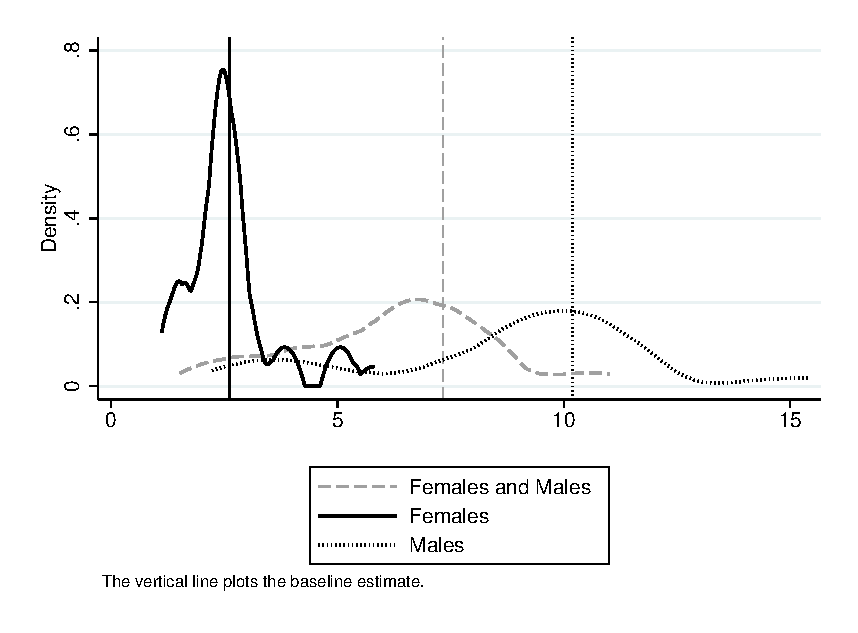
\includegraphics[width=\textwidth]{output/overalldist_BCRatio}
\end{subfigure}
\begin{subfigure}[h]{0.49\textwidth}
	\centering
	\caption{Internal Rate of Return} \label{fig:irr}
	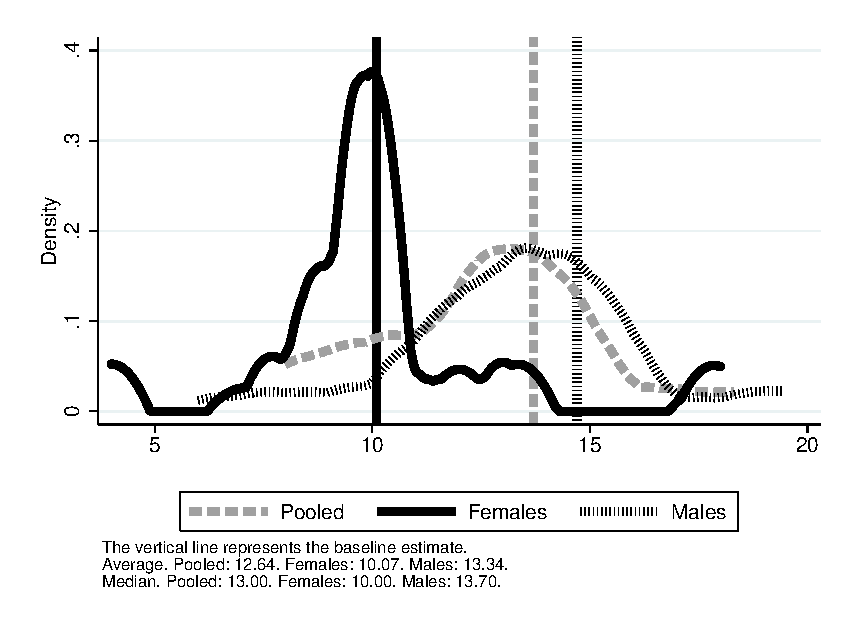
\includegraphics[width=\textwidth]{output/overalldist_IRR}
\end{subfigure}%
\footnotesize \justify
Note: Panel (a) displays the distribution of estimates of the benefit/cost ratio that we estimate throughout the paper. Vertical lines indicate the baseline estimates, presented in Figure~\ref{figure:main}. Panel (b) presents the analogous figure for the internal rate of return. See Figure~\ref{figure:ranges-NPV} in Appendix~\ref{appendix:sensitivity} for the analogous plots of net present values.
\end{sidewaysfigure}

\noindent This appendix evaluates how the estimates in the main paper vary as we alter certain sample selections from all of our data sources and other parameters. We first present plot of all net present value estimations across specifications in Figure~\ref{figure:ranges-NPV}. This is analogous to Figure~\ref{figure:ranges}.

\begin{figure}[H]
\centering
\caption{Distribution of Net Present Value Estimates}\label{figure:ranges-NPV}
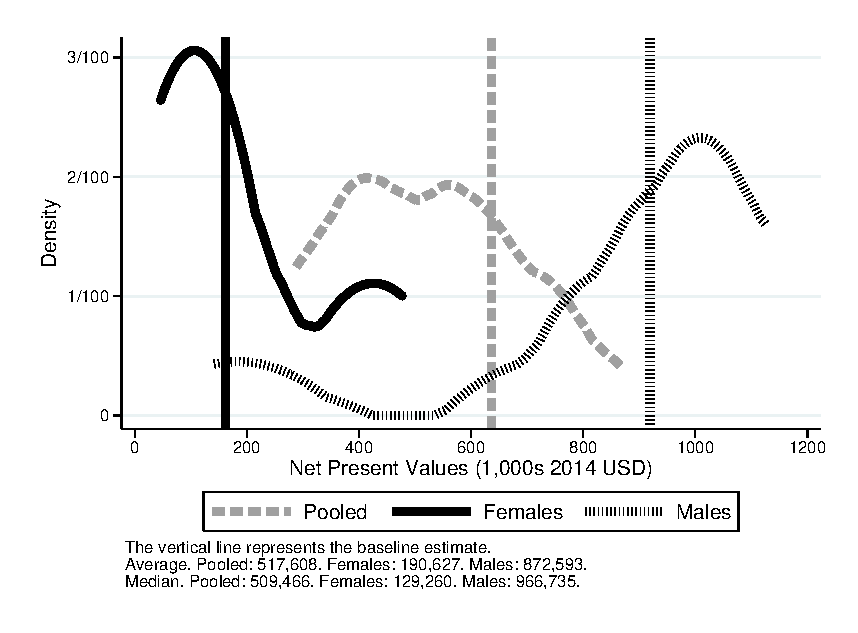
\includegraphics[width=\textwidth]{output/overalldist_npv}
\footnotesize \justify
Note: This figure displays the distribution of estimates of the net present value that we estimate throughout the paper. Vertical lines indicate the baseline estimates, presented in Figure~\ref{figure:main}. 
\end{figure}

\noindent We next analyze sensitivity due to (i) assumptions on the values of the discount rate; (ii) assumptions on the deadweight loss to society coming from taxes raised to fund public programs; and (iii) the magnitude of the components contributing to the benefit/cost ratio and internal rate of return. Table~\ref{table:cba} summarizes our sensitivity analysis. We conduct a rather drastic sensitivity analysis by removing components of the cost/benefit analysis entirely. Even when completely removing the gain associated with crime for males, the program is socially efficient---both the internal rate of return and the benefit/cost ratio are substantial. Parental labor income and crime are the components for which the internal rate of return and the benefit/cost ratio are the most sensitive. The reason for this sensitivity to parental labor income is that the amount is substantial and it is not heavily discounted because it accumulates during the first $21$ years of the subjects' lives. Crime occurs later in life and its benefits are discounted accordingly. The amount due to savings in crime is large, so removing it diminishes both the internal rate of return and the benefit/cost ratio (but they remain statistically significant).

\begin{table}[H]
\centering
\caption{Cost/Benefit Analysis of ABC/CARE, Summary}\label{table:cba}
\begin{threeparttable}
\tiny
\begin{tabular}{l r r r r r r r r r}																			
\toprule																			
&       \mc{3}{c}{Females}      &       \mc{3}{c}{Males}        &       \mc{3}{c}{Pooled}       \\																			
\cmidrule(lr){2-4}      \cmidrule(lr){5-7}      \cmidrule(lr){8-10}																			
Removed Component       &       NPV     &       IRR     &       B/C     &       NPV     &       IRR     &       B/C     &       NPV     &       IRR     &       B/C     \\																			
\midrule																			
None	&	161,759	&	\textbf{10.1\%}	&	\textbf{2.61}	&	919,049	&	\textbf{14.7\%}	&	\textbf{10.19}	&	636,674	&	\textbf{13.7\%}	&	\textbf{7.33}	\\
	&		&	(6\%)	&	(0.73)	&		&	(4\%)	&	(2.93)	&		&	(3\%)	&	(1.84)	\\ \\
Parental Income	&	148,854	&	4\%	&	1.12	&	107,907	&	\textbf{11\%}	&	\textbf{9.10}	&	116,953	&	\textbf{9\%}	&	\textbf{6.17}	\\
	&		&	(2\%)	&	(0.65)	&		&	(3\%)	&	(2.92)	&		&	(3\%)	&	(1.87)	\\
Subject Labor Income	&	41,908	&	9\%	&	\textbf{2.21}	&	238,105	&	\textbf{13\%}	&	\textbf{7.75}	&	133,032	&	\textbf{13\%}	&	\textbf{6.03}	\\
	&		&	(6\%)	&	(0.66)	&		&	(5\%)	&	(2.23)	&		&	(4\%)	&	(1.77)	\\
Subject Transfer Income	&	419	&	\textbf{10\%}	&	\textbf{2.61}	&	-7,265	&	\textbf{15\%}	&	\textbf{10.26}	&	-4,372	&	\textbf{14\%}	&	\textbf{7.38}	\\
	&		&	(6\%)	&	(0.73)	&		&	(4\%)	&	(2.93)	&		&	(3\%)	&	(1.84)	\\
Subject QALY	&	42,102	&	9\%	&	\textbf{2.20}	&	106,218	&	\textbf{14\%}	&	\textbf{9.14}	&	87,181	&	\textbf{13\%}	&	\textbf{6.48}	\\
	&		&	(6\%)	&	(0.69)	&		&	(6\%)	&	(2.73)	&		&	(5\%)	&	(1.79)	\\
Medical Expenditures	&	-16,037	&	9\%	&	\textbf{2.77}	&	-42,038	&	\textbf{15\%}	&	\textbf{10.61}	&	-31,221	&	\textbf{14\%}	&	\textbf{7.65}	\\
	&		&	(6\%)	&	(0.76)	&		&	(3\%)	&	(2.89)	&		&	(3\%)	&	(1.85)	\\
Alternative Preschools	&	16,691	&	8\%	&	\textbf{2.45}	&	13,434	&	\textbf{14\%}	&	\textbf{10.05}	&	14,659	&	\textbf{12\%}	&	\textbf{7.19}	\\
	&		&	(5\%)	&	(0.73)	&		&	(4\%)	&	(2.92)	&		&	(3\%)	&	(1.84)	\\
Education Costs	&	1,457	&	\textbf{10\%}	&	\textbf{2.59}	&	-7,852	&	\textbf{15\%}	&	\textbf{10.26}	&	-4,518	&	\textbf{14\%}	&	\textbf{7.37}	\\
	&		&	(6\%)	&	(0.72)	&		&	(4\%)	&	(2.93)	&		&	(3\%)	&	(1.86)	\\
Crime Costs	&	31,668	&	10\%	&	\textbf{2.34}	&	638,923	&	\textbf{9\%}	&	4.08	&	450,368	&	\textbf{8\%}	&	\textbf{3.06}	\\
	&		&	(6\%)	&	(0.62)	&		&	(5\%)	&	(2.18)	&	&	(4\%)	&	(1.01)	\\ \\
Deadweight Loss	&		&	\textbf{18\%}	&	\textbf{3.83}	&		&	\textbf{19\%}	&	\textbf{15.38}	&		&	\textbf{18\%}	&	\textbf{11.01}	\\
	&		&	(12\%)	&	(1.04)	&		&	(6\%)	&	(4.35)	&		&	(5\%)	&	(2.79)	\\
0\% Discount Rate	&		&		&	\textbf{5.06}	&		&		&	\textbf{25.45}	&		&		&	\textbf{17.40}	\\
	&		&		&	(2.82)	&		&		&	(10.42)	&		&		&	(5.90)	\\
7\% Discount Rate	&		&		&	\textbf{1.49}	&		&		&	\textbf{3.78}	&		&		&	\textbf{2.91}	\\
	&		&		&	(0.32)	&		&		&	(0.79)	&		&		&	(0.59)	\\
\bottomrule																			
\end{tabular}																			

\begin{tablenotes}
\footnotesize
\item Note: This table presents the estimates of the net present value (NPV) for each component, and the internal rate of return (IRR) and the benefit/cost ratio (B/C) of ABC/CARE for different scenarios based on comparing the groups randomly assigned to receive center-based childcare and the groups randomly assigned as control in ABC/CARE. The first row represents the baseline estimates. The other rows present estimates for scenarios in which we remove the NPV estimates of the component listed in the first column. The category ``Alternative Preschools'' refers to the money spent in alternatives to treatment from the control-group children parents. QALYs refers to the quality-adjusted life years. Any gain corresponds to better health conditions through the age of death. The quantity listed in the NPV columns is the component we remove from NPV when computing the calculation in each row. All the money figures are in 2014 USD and are discounted to each child's birth, unless otherwise specified. For the B/C ratio we use a discount rate of $3\%$, unless otherwise specified. We test the null hypotheses $\text{IRR} = 3\%$ and $\text{B/C} = 1$---we select $3\%$ as the benchmark null because that is the discount rate we use. Inference is based on non-parametric, one-sided $p$-values from the empirical bootstrap distribution. We highlight point estimates significant at the $10\%$ level. Total cost of the program per child is \$$92,570$ (2014).
\end{tablenotes}
\end{threeparttable}
\end{table}

\subsection{Varying the Discount Rate}
\label{appendix:varying-discount-rate}

%In this section we explore how the internal rate of return and benefit/cost ratio
%change when we adjust various components of the cash flow, as well as various parameters
%we assume. Not only does this provide us with an idea of how stable our estimates 
%are, but also which components or assumptions are responsible for any instabilities
%we find in our estimates.

\noindent Below we examine how the benefit/cost ratio is impacted by our choice of the discount rate. 

\noindent Figure \ref{fig:bcr_discount} displays how the benefit/cost ratio changes as we adjust
the rate at which we discount the cash flows. We find that for males, the benefits of 
the programs exceed the costs for discount rates as high as 15\%. We also
find that the benefit/cost ratios for discount rates of 2--12\% remain within the 
80\% confidence interval of our actual point estimate. The case is different for females,
for whom the ratio falls below 1 at a discount rate closer to 10\%. The benefit/cost ratio for 
females remain within the 80\% confidence interval of our estimate for discount rates
of 2--15\%. Although the alternate estimates generally remain within the 80\%
confidence intervals for both males and females, the slope of the curves in Figure
\ref{fig:bcr_discount} indicate that our estimates are sensitive to our choice of
the discount rate, especially for males. 

\begin{figure}[H]
\caption{Benefit/cost Ratio vs. Discount Rate} \label{fig:bcr_discount}
	\begin{subfigure}[h]{0.8\textwidth}
	\centering
	\caption{Females} \label{fig:bcr_discount_f1}
	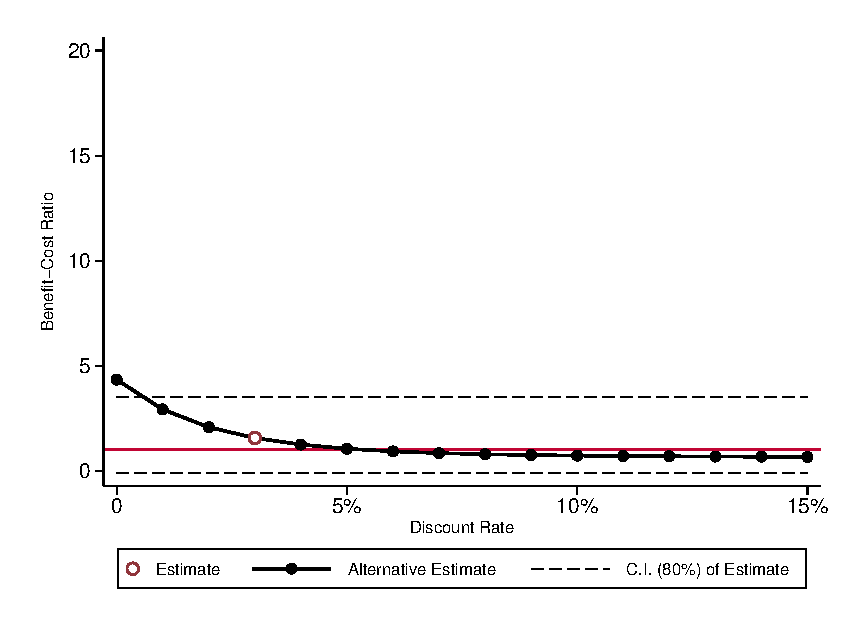
\includegraphics[width=\textwidth]{AppOutput/Sensitivity/bcr_discount_f1.eps}
	\end{subfigure}
	
	\begin{subfigure}[h]{0.8\textwidth}
	\centering
	\caption{Males} \label{fig:bcr_discount_m}
	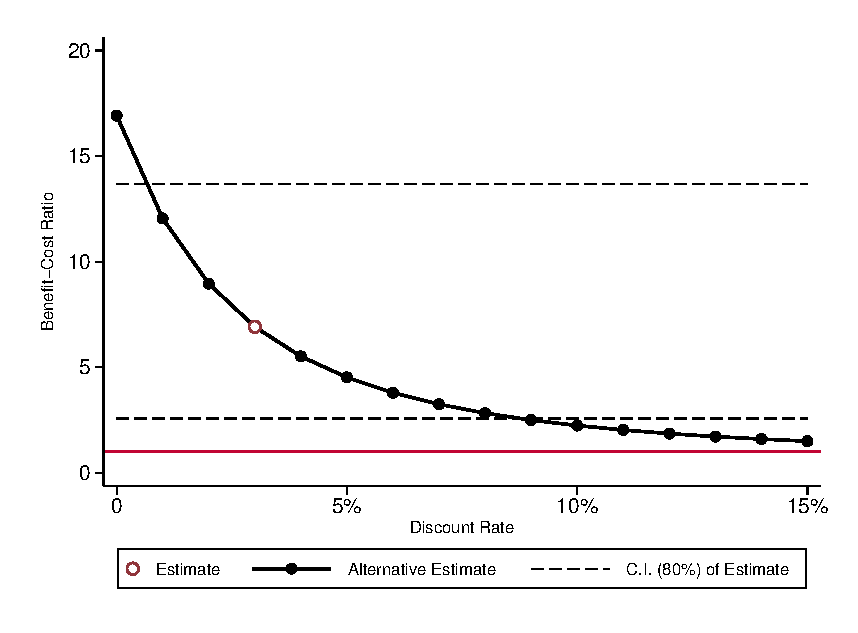
\includegraphics[width=\textwidth]{AppOutput/Sensitivity/bcr_discount_m1.eps}
	\end{subfigure}
	\floatfoot{
	\noindent Note: These graphs display how the benefit/cost ratios change
	for females and males as we vary the rate at which we discount to obtain the 
	present value. 
	The red line indicates a benefit/cost ratio of 1. 
	The hollow circle represents our actual estimates, whereas the
	solid dots represent the alternative estimates we obtain by varying the discount rate. 
	The estimates presented in the paper assume that the marginal 
	cost of welfare is \$0.50 for every dollar of tax revenue. 
	The estimates are means of the empirical bootstrap 
	distribution. The 80\% confidence intervals are obtained by taking the 10\textsuperscript{th}
	and 90\textsuperscript{th} quantiles of the bootstrap distribution.
	}
\end{figure}


\subsection{Varying Deadweight Loss}
\label{appendix:varying-dwl}

\noindent Below we examine how our estimates of the internal rate of return (IRR) and benefit/cost
ratios move with respect to changes in the marginal cost of welfare. 

\noindent Figure \ref{fig:irr_dwl} shows how the IRR changes as we adjust
the marginal cost of welfare. For both males and females, we find the IRRs
to be most sensitive at the lower marginal costs. The IRRs for both sexes
steadily decline as we increase the marginal cost of welfare to \$3 for every dollar
of tax revenue. This is likely due
to the fact that both females and males in treatment live longer, and are expected to 
receive more Medicare and Medicaid benefits in their later life. 
Also, we treat the costs of implementing ABC/CARE as a public cost. 
Thus, the steady increase in deadweight loss results in a 
steady decline in the IRR. Nonetheless, we see that the IRRs 
remain within the 80\% confidence interval of our original estimate 
for both females and males and are not particularly sensitive to changes within the 
neighborhood of our assumed marginal cost of welfare (note each point on the $x$-axis
represents a \$0.25 increment in the cost of welfare per dollar of tax revenue). 


\begin{figure}[H]
\caption{Internal Rate of Return vs. Deadweight Loss} \label{fig:irr_dwl}
	\begin{subfigure}[h]{0.8\textwidth}
	\centering
	\caption{Females} \label{fig:irr_dwl_f}
	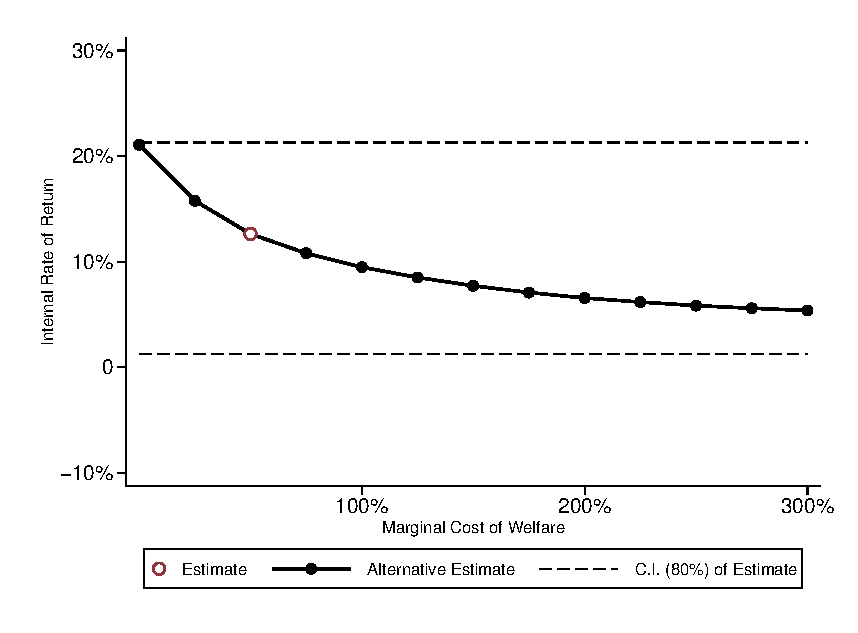
\includegraphics[width=\textwidth]{AppOutput/Sensitivity/irr_dwl_f1.eps}
	\end{subfigure}
	
	\begin{subfigure}[h]{0.8\textwidth}
	\centering
	\caption{Males} \label{fig:irr_dwl_m}
	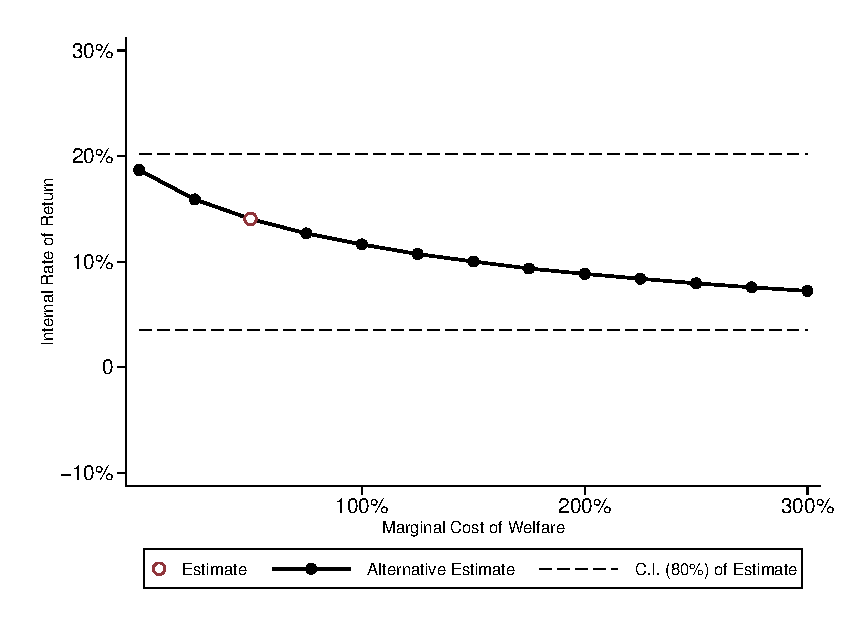
\includegraphics[width=\textwidth]{AppOutput/Sensitivity/irr_dwl_m1.eps}
	\end{subfigure}
	\floatfoot{
	\noindent Note: These graphs display how the internal rate of return changes
	for females and males as we vary the marginal cost of welfare.
	The hollow circle represents our actual estimates, whereas the
	solid dots represent the alternative estimates we obtain by varying the marginal
	cost of welfare. The estimates 
	presented in the paper assume that the marginal cost of welfare is \$0.50 for 
	every dollar of tax revenue. The estimates are means of the empirical bootstrap 
	distribution. The 80\% confidence intervals are obtained by taking the 10\textsuperscript{th}
	and 90\textsuperscript{th} quantiles of the bootstrap distribution.
	}
\end{figure}

\noindent Figure \ref{fig:bcr_dwl} illustrates how the benefit/cost ratio changes as we vary
the marginal cost of welfare. For females we see that the benefits exceed the costs (both are discounted at a rate of 4\%) even when the marginal cost of welfare is
assumed to equal \$3 for every dollar of tax revenue. We see a similar relationship hold for men, however, the ratio is significantly higher at every marginal cost.

\begin{figure}[H]
\caption{Benefit/cost Ratio vs. Deadweight Loss} \label{fig:bcr_dwl}
	\begin{subfigure}[h]{0.8\textwidth}
	\centering
	\caption{Females} \label{fig:bcr_dwl_f}
	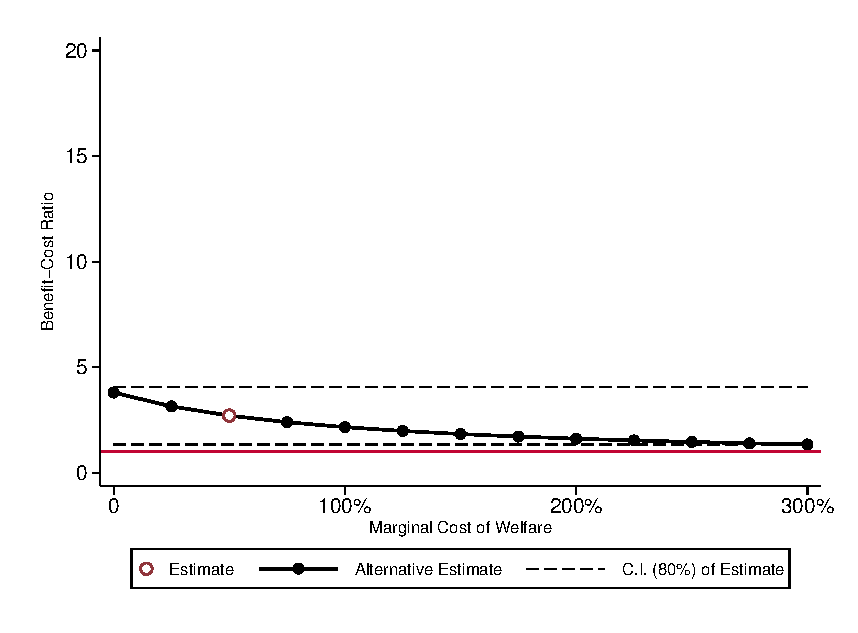
\includegraphics[width=\textwidth]{AppOutput/Sensitivity/bcr_dwl_f1.eps}
	\end{subfigure}
	
	\begin{subfigure}[h]{0.8\textwidth}
	\centering
	\caption{Males} \label{fig:bcr_dwl_m}
	\includegraphics[width=\textwidth]{AppOutput/Sensitivity/bcr_dwl_m1.eps}
	\end{subfigure}
	\floatfoot{
	\noindent Note: These graphs display how the benefit/cost ratio changes
	for females and males as we vary the marginal cost of welfare.  
	The red line indicates a benefit/cost ratio of 1. 
	The hollow circle represents our actual estimates, whereas the
	solid dots represent the alternative estimates we obtain by varying the marginal
	cost of welfare. The estimates 
	presented in the paper assume that the marginal cost of welfare is \$0.50 for 
	every dollar of tax revenue. The estimates are means of the empirical bootstrap 
	distribution. The 80\% confidence intervals are obtained by taking the 10\textsuperscript{th}
	and 90\textsuperscript{th} quantiles of the bootstrap distribution.
	}
\end{figure}

\subsection{Varying Component Magnitudes}
\label{app:sa_factors}

\noindent Below we explore how the internal rate of return (IRR) and benefit/cost ratio change as
we increase and decrease the value of each component of the benefit and cost streams. This entails
multiplying each component by factors ranging from 0 to 3. A factor of 0 is equivalent
to removing the component entirely from our analysis. In the particular
case of QALYs, the multiplicative factors correspond to different valuations of a year of perfect
health, e.g., a QALY equal to 1. For instance, as our current estimates assume a QALY of 1 to be worth
\$150,000, a factor of 0.5 corresponds to a year of perfect health being
worth \$75,000, and a factor of 3 corresponds to a year of perfect health
being worth \$450,000 (all values are in 2014 USD). 

\noindent Figure \ref{fig:irrf_factor_f} displays how the IRR for females
changes as we multiply each component by a factor between 0 and 3. We find that the IRR
is stable across different levels of public-transfer income, QALYs, health costs, and criminal 
costs. Parental income has the biggest effect on the IRR, 
and is one of the only components for which the alternative IRR falls outside of the 80\% confidence 
interval of the original estimate. This occurs when we double the parental income component in the
flow of benefits. 
%By tripling the component, we obtain an IRR exceeding 100\%, which we do not display in the chart above.
 This sensitivity is due to both the magnitude of the
treatment effect on parental income, as well as how the treatment effect took place
earlier in the ABC/CARE subjects' lives. The sensitivity of the IRR to the program costs
is also a result of the timing of the costs in the subjects lives. As females in the treatment groups attained higher levels of education
than females in the control groups, we observe that the IRR decreases as we multiply the
expenditure on education by increasingly large factors. On the other hand, this translates
to additional labor income for females, which we observe to have a positive effect on the
IRR. However, the IRR appears to be more sensitive to the costs of education relative
to labor income, as schooling costs are borne at earlier stages of each subject's life. 


\begin{figure}[H]
\caption{Internal Rate of Return vs.~Components, Females} \label{fig:irrf_factor_f}
	
	\begin{subfigure}[h]{0.8\textwidth}
	\centering
	\caption{Labor Income} \label{fig:irrf_inc_labor_f1}
	\includegraphics[width=\textwidth]{AppOutput/Sensitivity/irrf_inc_labor_f1.eps}
	\end{subfigure}
	
	\begin{subfigure}[h]{0.8\textwidth}
	\centering
	\caption{Public-Transfer Income} \label{fig:irrf_transfer_f1}
	\includegraphics[width=\textwidth]{AppOutput/Sensitivity/irrf_transfer_f1.eps}
	\end{subfigure}
\end{figure}

\begin{figure}[H]
\ContinuedFloat	
	\begin{subfigure}[h]{0.8\textwidth}
	\centering
	\caption{Parental Income} \label{fig:irrf_inc_parent_f1}
	\includegraphics[width=\textwidth]{AppOutput/Sensitivity/irrf_inc_parent_f1.eps}
	\end{subfigure}
	
	\begin{subfigure}[h]{0.8\textwidth}
	\centering
	\caption{Quality-Adjusted Life Years} \label{fig:irrf_qaly_f1}
	\includegraphics[width=\textwidth]{AppOutput/Sensitivity/irrf_qaly_f1.eps}
	\end{subfigure}
\end{figure}
	
\begin{figure}[H]
\ContinuedFloat	
	\begin{subfigure}[h]{0.8\textwidth}
	\centering
	\caption{Health Costs} \label{fig:irrf_health_f1}
	\includegraphics[width=\textwidth]{AppOutput/Sensitivity/irrf_health_f1.eps}
	\end{subfigure}
	
	\begin{subfigure}[h]{0.8\textwidth}
	\centering
	\caption{Education Costs} \label{fig:irrf_edu_f1}
	\includegraphics[width=\textwidth]{AppOutput/Sensitivity/irrf_edu_f1.eps}
	\end{subfigure}
\end{figure}

\begin{figure}[H]
\ContinuedFloat	
	\begin{subfigure}[h]{0.8\textwidth}
	\centering
	\caption{Crime Costs} \label{fig:irrf_crime_f1}
	\includegraphics[width=\textwidth]{AppOutput/Sensitivity/irrf_crime_f1.eps}
	\end{subfigure}
	
	\begin{subfigure}[h]{0.8\textwidth}
	\centering
	\caption{Program Costs} \label{fig:irrf_costs_f1}
	\includegraphics[width=\textwidth]{AppOutput/Sensitivity/irrf_costs_f1.eps}
	\end{subfigure}
\end{figure}
	
\begin{figure}[H]
\ContinuedFloat	
	\begin{subfigure}[h]{0.8\textwidth}
	\centering
	\caption{Control Substitution Costs} \label{fig:irrf_cc_f1}
	\includegraphics[width=\textwidth]{AppOutput/Sensitivity/irrf_cc_f1.eps}
	\end{subfigure}
	
	\floatfoot{
	\noindent Note: These graphs display how the internal rate of return changes
	for females as we multiply each component by a factor from 0 to 3. 
	The hollow circle represents our actual estimates, whereas the
	solid dots represent the alternative estimates we obtain by varying the 
	magnitude of each component. The estimates 
	presented in the paper are equal to the IRRs presented above when the multiplicative
	factor is equal to 1. The estimates are means of the empirical bootstrap 
	distribution. The 80\% confidence intervals are obtained by taking the 10\textsuperscript{th}
	and 90\textsuperscript{th} quantiles of the bootstrap distribution.
	}
\end{figure}

\noindent Figure \ref{fig:irrf_factor_m} displays how the IRR for males changes as we vary the magnitude
of each component of the benefits and costs. Our findings for males are similar to
those for females: the IRR is insensitive to changes in public-transfer income, QALYs, and health costs. 
As the parental income and the program cost components for the female subsample is 
the same as those of the male subsample, we also observe that the IRR for males 
is sensitive to changes in both of these components. The IRR for males is not sensitive to increasing the weight of the cost of control substitution and responds to increases in costs at a smaller rate than females. 
%Compared to females, however, as the weight increases, the internal rate of return increases at a much faster rate.
This is a product of the different populations of males and females who were enrolled in alternative preschools.
The IRR for the male subsample is a little less sensitive to changes in labor income
than for the female subsample, but we still observe in Figure \ref{fig:irrf_factor_m}
that the IRR for males rises as we multiply the benefits stemming from this component by increasingly large factors. 
Finally, the IRR 
increases for males as we increase the magnitude of the criminal cost component. 
This is not surprising because the reduction in the costs of crimes is the largest 
benefit of ABC/CARE for males. 


\begin{figure}[H]
\caption{Internal Rate of Return vs.~Components, Males} \label{fig:irrf_factor_m}
	\begin{subfigure}[h]{0.8\textwidth}
	\centering
	\caption{Labor Income} \label{fig:irrf_inc_labor_m1}
	\includegraphics[width=\textwidth]{AppOutput/Sensitivity/irrf_inc_labor_m1.eps}
	\end{subfigure}	
	
	\begin{subfigure}[h]{0.8\textwidth}
	\centering
	\caption{Public-Transfer Income} \label{fig:irrf_transfer_m1}
	\includegraphics[width=\textwidth]{AppOutput/Sensitivity/irrf_transfer_m1.eps}
	\end{subfigure}
\end{figure}
	
\begin{figure}[H]
\ContinuedFloat		
	\begin{subfigure}[h]{0.8\textwidth}
	\centering
	\caption{Parental Income} \label{fig:irrf_inc_parent_m1}
	\includegraphics[width=\textwidth]{AppOutput/Sensitivity/irrf_inc_parent_m1.eps}
	\end{subfigure}
	
	\begin{subfigure}[h]{0.8\textwidth}
	\centering
	\caption{Quality-Adjusted Life Years} \label{fig:irrf_qaly_m1}
	\includegraphics[width=\textwidth]{AppOutput/Sensitivity/irrf_qaly_m1.eps}
	\end{subfigure}
\end{figure}
	
\begin{figure}[H]
\ContinuedFloat		
	\begin{subfigure}[h]{0.8\textwidth}
	\centering
	\caption{Health Costs} \label{fig:irrf_health_m1}
	\includegraphics[width=\textwidth]{AppOutput/Sensitivity/irrf_health_m1.eps}
	\end{subfigure}
	
	\begin{subfigure}[h]{0.8\textwidth}
	\centering
	\caption{Education Costs} \label{fig:irrf_edu_m1}
	\includegraphics[width=\textwidth]{AppOutput/Sensitivity/irrf_edu_m1.eps}
	\end{subfigure}
\end{figure}
	
\begin{figure}[H]
\ContinuedFloat		
	\begin{subfigure}[h]{0.8\textwidth}
	\centering
	\caption{Crime Costs} \label{fig:irrf_crime_m1}
	\includegraphics[width=\textwidth]{AppOutput/Sensitivity/irrf_crime_m1.eps}
	\end{subfigure}
	
	\begin{subfigure}[h]{0.8\textwidth}
	\centering
	\caption{Program Costs} \label{fig:irrf_costs_m1}
	\includegraphics[width=\textwidth]{AppOutput/Sensitivity/irrf_costs_m1.eps}
	\end{subfigure}
\end{figure}
	
\begin{figure}[H]
\ContinuedFloat		
	\begin{subfigure}[h]{0.8\textwidth}
	\centering
	\caption{Control Substitution Costs} \label{fig:irrf_cc_m1}
	\includegraphics[width=\textwidth]{AppOutput/Sensitivity/irrf_cc_m1.eps}
	\end{subfigure}
	
	\floatfoot{
	\noindent Note: These graphs display how the internal rate of return changes
	for males as we multiply each component by a factor from 0 to 3. 
	The hollow circle represents our actual estimates, whereas the
	solid dots represent the alternative estimates we obtain by varying the 
	magnitude of each component. The estimates 
	presented in the paper are equal to the IRRs presented above when the multiplicative
	factor is equal to 1. The estimates are means of the empirical bootstrap 
	distribution. The 80\% confidence intervals are obtained by taking the 10\textsuperscript{th}
	and 90\textsuperscript{th} quantiles of the bootstrap distribution.
	}
\end{figure}

\noindent Figure \ref{fig:bcrf_factor_f} shows how the benefit/cost ratio changes for females as
we multiply each component of the benefits and costs by a factor between 0 and 3. We 
observe that the ratio is generally insensitive to changes in all the components, 
except parental income, labor income, education costs, crime costs, and program costs. The sensitivity
to program costs is due to the fact that it is the denominator of the 
benefit/cost ratio. In the case of the other components, when discounted, 
they exhibit the largest present values. The sensitivity of the benefit/cost
ratio to changes in these components therefore indicates the magnitude of those 
components relative to the rest, with parental income having the largest magnitude
in terms of discounted treatment effect, followed by labor income, and then
education costs. 

\begin{figure}[H]
\caption{Benefit/cost Ratio vs.~Components, Females} \label{fig:bcrf_factor_f}

	\begin{subfigure}[h]{0.8\textwidth}
	\centering
	\caption{Labor Income} \label{fig:bcrf_inc_labor_f1}
	\includegraphics[width=\textwidth]{AppOutput/Sensitivity/bcrf_inc_labor_f1.eps}
	\end{subfigure}	
	
	\begin{subfigure}[h]{0.8\textwidth}
	\centering
	\caption{Public-Transfer Income} \label{fig:bcrf_transfer_f1}
	\includegraphics[width=\textwidth]{AppOutput/Sensitivity/bcrf_transfer_f1.eps}
	\end{subfigure}
\end{figure}
	
\begin{figure}[H]
\ContinuedFloat		
	\begin{subfigure}[h]{0.8\textwidth}
	\centering
	\caption{Parental Income} \label{fig:bcrf_inc_parent_f1}
	\includegraphics[width=\textwidth]{AppOutput/Sensitivity/bcrf_inc_parent_f1.eps}
	\end{subfigure}
	
	\begin{subfigure}[h]{0.8\textwidth}
	\centering
	\caption{Quality-Adjusted Life Years} \label{fig:bcrf_qaly_f1}
	\includegraphics[width=\textwidth]{AppOutput/Sensitivity/bcrf_qaly_f1.eps}
	\end{subfigure}
\end{figure}
	
\begin{figure}[H]
\ContinuedFloat		
	\begin{subfigure}[h]{0.8\textwidth}
	\centering
	\caption{Health Costs} \label{fig:bcrf_health_f1}
	\includegraphics[width=\textwidth]{AppOutput/Sensitivity/bcrf_health_f1.eps}
	\end{subfigure}
	
	\begin{subfigure}[h]{0.8\textwidth}
	\centering
	\caption{Education Costs} \label{fig:bcrf_edu_f1}
	\includegraphics[width=\textwidth]{AppOutput/Sensitivity/bcrf_edu_f1.eps}
	\end{subfigure}
\end{figure}

\begin{figure}[H]
\ContinuedFloat			
	\begin{subfigure}[h]{0.8\textwidth}
	\centering
	\caption{Crime Costs} \label{fig:bcrf_crime_f1}
	\includegraphics[width=\textwidth]{AppOutput/Sensitivity/bcrf_crime_f1.eps}
	\end{subfigure}
	
	\begin{subfigure}[h]{0.8\textwidth}
	\centering
	\caption{Program Costs} \label{fig:bcrf_costs_f1}
	\includegraphics[width=\textwidth]{AppOutput/Sensitivity/bcrf_costs_f1.eps}
	\end{subfigure}
\end{figure}
	
\begin{figure}[H]
\ContinuedFloat		
	\begin{subfigure}[h]{0.8\textwidth}
	\centering
	\caption{Control Substitution Costs} \label{fig:bcrf_cc_f1}
	\includegraphics[width=\textwidth]{AppOutput/Sensitivity/bcrf_cc_f1.eps}
	\end{subfigure}
	
	\floatfoot{
	\noindent Note: These graphs display how the benefit/cost ratio changes
	for females as we multiply each component by a factor from 0 to 3. 
	The red line indicates a benefit/cost ratio of 1. 
	The hollow circle represents our actual estimates, whereas the
	solid dots represent the alternative estimates we obtain by varying the 
	magnitude of each component. The benefit/cost ratio 
	presented in the paper is equal to those presented above when the multiplicative
	factor is equal to 1. The estimates are means of the empirical bootstrap 
	distribution. The 80\% confidence intervals are obtained by taking the 10\textsuperscript{th}
	and 90\textsuperscript{th} quantiles of the bootstrap distribution.
	}
\end{figure}

\noindent Figure \ref{fig:bcrf_factor_m} displays how the benefit/cost ratio for males varies
as we multiply each component of the benefits and costs by a factor between 0 and 3.
We observe that the ratio is insensitive to the scaling of public-transfer income, health costs,
education costs, and control substitution costs. Barring program costs, the components that
vary the benefit/cost ratio the most are crime costs, parental income, labor income,
health expenditure, and QALYs, in that order. This is simply a result of the relevant 
magnitude of each of those components in the benefits stream after discounting. 


\begin{figure}[H]
\caption{Benefit/cost Ratio vs.~Components, Males} \label{fig:bcrf_factor_m}
	
	\begin{subfigure}[h]{0.8\textwidth}
	\centering
	\caption{Labor Income} \label{fig:bcrf_inc_labor_m1}
	\includegraphics[width=\textwidth]{AppOutput/Sensitivity/bcrf_inc_labor_m1.eps}
	\end{subfigure}
	
	\begin{subfigure}[h]{0.8\textwidth}
	\centering
	\caption{Public-Transfer Income} \label{fig:bcrf_transfer_m1}
	\includegraphics[width=\textwidth]{AppOutput/Sensitivity/bcrf_transfer_m1.eps}
	\end{subfigure}
\end{figure}

\begin{figure}[H]
\ContinuedFloat		
	\begin{subfigure}[h]{0.8\textwidth}
	\centering
	\caption{Parental Income} \label{fig:bcrf_inc_parent_m1}
	\includegraphics[width=\textwidth]{AppOutput/Sensitivity/bcrf_inc_parent_m1.eps}
	\end{subfigure}
	
	\begin{subfigure}[h]{0.8\textwidth}
	\centering
	\caption{Quality-Adjusted Life Years} \label{fig:bcrf_qaly_m1}
	\includegraphics[width=\textwidth]{AppOutput/Sensitivity/bcrf_qaly_m1.eps}
	\end{subfigure}
\end{figure}


\begin{figure}[H]
\ContinuedFloat	
	\begin{subfigure}[h]{0.8\textwidth}
	\centering
	\caption{Health Costs} \label{fig:bcrf_health_m1}
	\includegraphics[width=\textwidth]{AppOutput/Sensitivity/bcrf_health_m1.eps}
	\end{subfigure}
	
	\begin{subfigure}[h]{0.8\textwidth}
	\centering
	\caption{Education Costs} \label{fig:bcrf_edu_m1}
	\includegraphics[width=\textwidth]{AppOutput/Sensitivity/bcrf_edu_m1.eps}
	\end{subfigure}
\end{figure}	


\begin{figure}[H]
\ContinuedFloat		
	\begin{subfigure}[h]{0.8\textwidth}
	\centering
	\caption{Crime Costs} \label{fig:bcrf_crime_m1}
	\includegraphics[width=\textwidth]{AppOutput/Sensitivity/bcrf_crime_m1.eps}
	\end{subfigure}
	
	\begin{subfigure}[h]{0.8\textwidth}
	\centering
	\caption{Program Costs} \label{fig:bcrf_costs_m1}
	\includegraphics[width=\textwidth]{AppOutput/Sensitivity/bcrf_costs_m1.eps}
	\end{subfigure}
\end{figure}

	
\begin{figure}[H]
\ContinuedFloat		
	\begin{subfigure}[h]{0.8\textwidth}
	\centering
	\caption{Control Substitution Costs} \label{fig:bcrf_cc_m1}
	\includegraphics[width=\textwidth]{AppOutput/Sensitivity/bcrf_cc_m1.eps}
	\end{subfigure}
	
	\floatfoot{
	\noindent Note: These graphs display how the benefit/cost ratio changes
	for males as we multiply each component by a factor from 0 to 3. 
	The red line indicates a benefit/cost ratio of 1. 
	The hollow circle represents our actual estimates, whereas the
	solid dots represent the alternative estimates we obtain by varying the 
	magnitude of each component. The benefit/cost ratio 
	presented in the paper is equal to those presented above when the multiplicative
	factor is equal to 1. The estimates are means of the empirical bootstrap 
	distribution. The 80\% confidence intervals are obtained by taking the 10\textsuperscript{th}
	and 90\textsuperscript{th} quantiles of the bootstrap distribution.
	}
\end{figure}

\noindent Overall, we find that the benefit/cost ratio is stable across changes in the data, 
as well as changes in our assumptions regarding the discount rate and the marginal
cost of welfare. The IRR tends to be more sensitive to changes in the data
and assumptions.


\setcounter{figure}{0}  \renewcommand{\thefigure}{Q.\arabic{figure}}
\setcounter{table}{0}   \renewcommand{\thetable}{Q.\arabic{table}}

\section{Back-of-the-Envelope Cost Benefit Analysis of ABC} \label{appendix:back}

\noindent This section presents a back-of-the-envelope cost-benefit analysis in a similar spirit to that of \citet{Chetty_Friedman_etal_2010_HowDoesYour} and \citet{Kline-Walters_2015_NBER-Evaluating}. The implementation is straightforward and it is based on the argument of  \citet{Chetty_Friedman_etal_2010_HowDoesYour} that a standard deviation in a kindergarten IQ score generates an increase of $13.1\%$ in earnings at age 27.\\

\noindent We perform two exercises. First, one similar to that of \citet{Kline-Walters_2015_NBER-Evaluating}. We calculate the treatment effect of ABC on a kindergarten IQ test---Wechsler Preschool and Primary Scale of Intelligence at Age 5, $\widehat{\Delta}$, and let the (discounted to age 5) life-cycle earnings in 2014 USD dollars be $\$460,793.34$. We take this number straight from \citet{Kline-Walters_2015_NBER-Evaluating}. Based on this, we calculate the total benefits induced by the program as: 

\begin{equation}
B = 460,793.34 \left( \widehat{\Delta} R_{IQ}  N_{\text{Treated}}  -  N_{\text{Control}} \right) , 
\end{equation}

\noindent where $N_{\text{Treated}}$ is the number of subjects in the treatment group and $N_{\text{Control}}$ is the number of subjects in the control group. $R_{IQ}$ is the earnings return to a standard deviation increase in a kindergarten IQ test---13.1\% in the case of \citep{Chetty_Friedman_etal_2010_HowDoesYour}. Then, we let the total cost of the program (discounted to age 5) be $\$5,893,093.20$, as documented in Appendix~\ref{app:programcosts}. We denote this by $C$.\\ 

\noindent For the program to break-even with respect to costs and benefits, a much higher return to the kindergarten IQ test is needed than the one reported in \citep{Chetty_Friedman_etal_2010_HowDoesYour}, $13.1\%$ vs. $40\%$. Figure~\ref{figure:first} plots the relationship between the $B/C$ and various values of $R_{IQ}$.\\ 

\noindent Next, we perform a similar calculation. Instead of letting $R_{IQ}$ vary, we fix it to $13.1\%$ and let the net present value of earnings over the life cycle vary. For the program to break even, this value needs to be beyond a million dollars (Figure~\ref{figuresecond}). \citet{Kline-Walters_2015_NBER-Evaluating} argue that this value is $\$359,064.50$ for disadvantaged populations in the U.S.

\begin{center}
\begin{figure}[H] 
\caption{Benefit-to-cost Ratio and the Earnings Returns to a Kindergarten IQ Test} \label{figure:first}
\centering
\includegraphics[width=.65\columnwidth]{Output/abc_chettytype_return.eps}
\floatfoot{
\footnotesize
Note: Benefit-to-cost ratio as a function of diverse earnings-returns to a standard deviation of a kindergarten IQ test.
}
\end{figure}
\end{center}

\begin{center}
\begin{figure}[H] 
\caption{Benefit-to-cost Ratio and the Discounted Net Present Value of Earnings}
\label{figuresecond}
\centering
\includegraphics[width=.65\columnwidth]{Output/abc_chettytype_pv.eps}
\floatfoot{
\footnotesize
Note: Benefit-to-cost ratio as a function of diverse net present value of earnings.
}
\end{figure}
\end{center}

\end{appendices}

%References
\renewcommand{\refname}{Appendix References}
\clearpage
\singlespace
\bibliographystyle{chicago}
\bibliography{heckman}

\end{document} 